\documentclass[a4paper,titlepage,UTF8,zhihao=5]{ctexbook}

% 导言区

\usepackage[colorlinks, linkcolor=blue!50!black]{hyperref}  % 超链接的颜色设置为红色
\usepackage{xcolor}
\usepackage{listings}
\usepackage{geometry}
\usepackage{fancyhdr}
\usepackage{cite}
\usepackage[super]{gbt7714} % 中文文献包
\usepackage{graphicx} % 导入图片包
\usepackage{epstopdf} % 支持 eps
\graphicspath{{img/game/},{img/install/},{img/screenfetch/}}
\usepackage{subfig}
\usepackage{tabularx}
\usepackage{chngpage}
\usepackage{array}
\usepackage{parskip}
\usepackage{booktabs}
\usepackage{longtable}
\usepackage{makecell} % 表格
\usepackage{pbox}
\usepackage{graphicx} % 导入图片包
\graphicspath{{img/}}
\usepackage[bodytextleadingratio=1.45]{zhlineskip}
\usepackage{paralist}
\usepackage{adjustbox}
\usepackage{lstfiracode}
\usepackage{minted}
\usepackage[normalem]{ulem} % 定义文本高亮
\usepackage[toc]{multitoc} % 双栏目录
% 定义需要强调的环境
\newenvironment{notice}[1][注意]{{\textbf{#1}:}}

\newenvironment{seeAlso}[1][另请参阅]{{\textbf{#1}:}}

\newenvironment{warning}[1][警告]{{\textbf{#1}:}}

% 定义文本高亮
\newcommand\hl{\bgroup\markoverwith
  {\textcolor{yellow}{\rule[-.5ex]{2pt}{2.5ex}}}\ULon}

% 定义分隔线的样式
% \dotfill: 虚线
% \hrulefill: 实线
\newcommand{\splitLine}{\dotfill}

% 行内高度
\newcommand{\lineHigh}{\vspace{2em}}

% 不输出标题编号
\newcommand\specialsectioning{\setcounter{secnumdepth}{-1}}
\ctexset{section/format += \raggedright}

% \newfontfamily\consolas{Fira Code}
\newfontfamily\consolas{Source Code Pro}
% \newfontfamily\consolas{JetBrainsMono-Regular}

% green
\definecolor{mygreen}{rgb}{0, 0.6, 0}
% 设定版本宽度和高度
\geometry{papersize={35cm, 25cm}}
% 页边距
\geometry{left=2.5cm,right=2.5cm,top=2.0cm,bottom=2cm}

% 页眉页脚
\pagestyle{empty}

% 设定代码环境
\newfontfamily\fira{Fira Code}
\lstset{
	basicstyle=\small\fira,
	numberstyle= \tiny\fira, 
	keywordstyle= \color{ blue!70},
	commentstyle=\color{mygreen},
	frame=shadowbox, 
	rulesepcolor= \color{ red!20!green!20!blue!20},
	columns=flexible, 
	% linewidth=1.1\linewidth,
	linewidth=\linewidth,
} 


% 定义表格列宽
\newcolumntype{L}[1]{>{\vspace{0.5em}\begin{minipage}{#1}\raggedright\let\newline\\
\arraybackslash\hspace{0pt}}m{#1}<{\end{minipage}\vspace{0.5em}}}
\newcolumntype{R}[1]{>{\vspace{0.5em}\begin{minipage}{#1}\raggedleft\let\newline\\
\arraybackslash\hspace{0pt}}m{#1}<{\end{minipage}\vspace{0.5em}}}
\newcolumntype{C}[1]{>{\vspace{0.5em}\begin{minipage}{#1}\centering\let\newline\\
\arraybackslash\hspace{0pt}}m{#1}<{\end{minipage}\vspace{0.5em}}}

% 中文设置
\setCJKmainfont{SourceHanSerifCN-Light}

% 英文设置
% \setmainfont{JetBrains Mono}
\setmainfont{Source Code Pro}

% 标题页
\title{Qt中文文档翻译}
\author{作者:\href{https://github.com/QtDocumentCN}{QtDocumentCN}}
\ctexset{ today = small }
% 标题左对齐
\CTEXsetup[format={\Large}]{section}
% \ctexset{ section = {format = {\Large}}
\ctexset{
% chapter/format = \sffamily\raggedright,
section/format += \sffamily\Large,
% subsection/format += \fbox,
}
% 首行缩进两个字符
%\setlength{\parindent}{2em}
%\CTEXindent 
\CTEXnoindent % 取消首行缩进

\setlength{\headheight}{20pt}

\begin{document}
% 正文区(文稿区)
% 页眉页脚
\pagestyle{fancy}
\lhead{
\includegraphics[scale=0.1]{logo}}
\renewcommand{\headrulewidth}{0.4pt}

\maketitle
\tableofcontents
\thispagestyle{empty}
\newpage
\setcounter{page}{1}

% 不输出标题编号
\specialsectioning

\chapter{API Design Principles}

API 设计规范

\begin{quote}
译者注:

本文不来自于 Qt 文档,而是来自于 Qt Wiki:\href{https://wiki.qt.io/API_Design_Principles}{API\_Design\_Principles}

API(Application Programming Interface),应用开发接口,本文中也将 P 解释为 Programmer(开发者)。	
\end{quote}

Qt 最出名的特点之一是一致性强、易于学习、功能强大的 API。本文尝试对我们在设计 Qt 风格的 API 中积累的诀窍进行总结。其中许多准则都是通用的,其它的则是习惯性用法,我们主要为了保持接口一致性而继续遵循。

尽管这些准则主要面向公共接口,但也鼓励您在设计内部接口时使用相同的技术,这对与您合作开发的同僚会更加友好。

您可能也会有兴趣查阅 Jasmin Blanchette 的 
\href{https://people.mpi-inf.mpg.de/~jblanche/api-design.pdf}{Little Manual of API Design (PDF)},或它的前身,由 Matthias Ettrich 编写的 \href{https://doc.qt.io/archives/qq/qq13-apis.html}{Designing Qt-Style C++ APIs} 。

优秀接口的六大特点

API 是面向开发者的,而 GUI 则是面向终端用户。API 中的 P 代表开发者(Programmer),而非程序(Program),目的是指出 API 由开发者,即人类(而非计算机)所使用这一特点。

Matthias 在 Qt 季刊弟13期,关于 API 设计的文章中,声称他坚信 API 应该是最小化但完备的,具备清晰而简洁的语义,符合直觉,被开发者,易于记忆,能够引导开发者编写高可读性的代码。

最小化

最小化的 API 指包含尽可能少的公共成员和最少的类。这可让 API 更易于理解、记忆、调试和修改。

完备性
完备的 API 意味着具备所有应有的功能。这可能会与最小化产生冲突。此外,若一个成员函数位于错误的类中,则大多数潜在的用户回无法找到它。

清晰简洁的语义

与其它设计协作时,应该让您的设计做到最小例外。通用化会让事情更简单。特例可能存在,但不应成为关注的焦点。在处理特定问题时,不应让解决方案过度泛化。(例如,Qt 3 中的 QMineSourceFactory 本该被称作 QImageLoader,并且具备另一套 API。)

复合直觉

如同计算机上其它内容,API 应复合直觉。不同的开发经验和技术背景会导致对复合直觉与否有不同的感知。复合直觉的 API 应能让中等经验的开发者无需阅读文档并直接使用,并让不知道这个 API 的开发者可以理解使用它编写的代码。

易于记忆

为了让 API 易于记忆,请选择一组保持一致并足够精确的命名约定。使用可理解的模式和概念,并且避免缩写。

可读性导向

编写代码只需要一次,但阅读(以及调试和修改)则会非常频繁。高可读性的代码通常需要花更多时间编写,但可以在产品的生命周期中节约更多的时间。

最后需要谨记,不同类型的用户会使用 API 的不同部分。在单纯地创建一个 Qt 类实例能非常直观的同时,希望用户在尝试继承它之前先阅读文档则是很合理的。

静态多态

相似的代码类应具有相似的 API。可以使用继承来实现——当运行时多态支持时,这是很合理的。但多态同时也可以体现在设计截断。例如,若将代码中的 QProgressBar 换为 QSlider,或将 QString 换为 QByteArray,他们间相似的 API 会另替换操作变得非常容易。这便是为何我们称之为“静态多态”。

静态多态同样可让记忆 API 和开发模式变得更加简单。结果是,对于一组有关联的类,相似的 API 通常比为每个类独立设计的完美 API 更加好用。

在 Qt 中,当不具备有足够说服力的原因时,我们更倾向于使用静态多态,而非继承。这减少了 Qt 的公共类数量,并让新用户更容易在文档中找到需要的内容。

好的

​ QDialogBox 和 QMessageBox 具有相似的 APi,以用于处理按钮(addButton(), setStandardButtons(),但无需继承自某些 "QAbstractButtonBox" 类。

坏的

​ QAbstractSocket 被 QTcpSOcket 和 QUdpSocket 所继承,但这两个类的交互方式差异很大。看起来并没有人使用过(或能够使用) QAbstractSocket 指针来进行通用且有效的操作。

存疑

​ QBoxLayout 是 QHBoxLayout 和 QVBoxLayout 的基类。优点:可以在工具栏中使用 QBoxLayout,调用 setOrientation() 来令其水平/垂直排布。缺点:引入额外的类,用户可能会写出形如 ((QBoxLayout *)hbox)->setOrientation(Qt::Vertical) 的代码,而这是不合理的。

基于属性的 API
比较新的 Qt 类倾向于使用基于属性的 API,例如:

\begin{lstlisting}
QTimer timer;
timer.setInterval(1000);
timer.setSingleShot(true);
timer.start(); 
\end{lstlisting}

此处的属性,指的是作为对象状态一部分的任何概念性的特征——无论是否是实际的 Q\_PROPERTY。只要可行,用户都应该允许以任何顺序设置属性,也就是说,这些属性应该是正交的。例如,上文的代码也可以写为:

\begin{lstlisting}
QTimer timer;
timer.setSingleShot(true);
timer.setInterval(1000);
timer.start(); 
\end{lstlisting}

为了方便,我们也可以这样写:

\begin{lstlisting}
timer.start(1000);
\end{lstlisting}

类似的,对于 QRegExp,我们可以:

\begin{lstlisting}
QRegExp regExp;
regExp.setCaseSensitive(Qt::CaseInsensitive);
regExp.setPattern(".");
regExp.setPatternSyntax(Qt::WildcardSyntax);
\end{lstlisting}

为了实现此类 API,内部的对象需要被惰性构造。例如在 QRegExp 的案例中,不应该在还不知道表达式使用何种语法之前,就在 setPattern() 中过早地编译 . 表达式。

属性通常是级联的,此时我们应该谨慎地处理。仔细考虑下当前样式提供的“默认图标大小”与 QToolButton 的 iconSize 属性:

\begin{lstlisting}
toolButton->iconSize(); // 返回当前样式表的默认大小
toolButton->setStyle(otherStyle);
toolButton->iconSize(); // 返回 otherStyle 的默认大小
toolButton->setIconSize(QSize(52, 52));
toolButton->iconSize(); // 返回 (52, 52)
toolButton->setStyle(yetAnotherStyle);
toolButton->iconSize(); // 返回 (52, 52) 
\end{lstlisting}


注意,一旦 iconSize 被设置,它会被一直留存,此时修改当前样式不会影响它。这是 好的。有时,提供重置属性的渠道会很方便,这有两种实现方式:

\begin{itemize}
	\item 传递一个特定值(如 QSIze()、-1 或 Qt::Alignment(0))来指代“重置”;
	\item 提供显示的 resetFoo() 或 unsetFoo() 函数。
\end{itemize}

对于 iconSize,将 QSize()(即 QSize(-1, -1))设为“重置”便足够了。

某些场景中,取值方法会返回值会与设置的内容不同。例如,若调用 widget->setEnabled(true),可能通过 widget->isEnabled() 获得的依然是 false,因为父控件被禁用了。这并没问题,因为通常这正是我们要检查的状态(父控件被禁用时,子控件也应该变灰,表现为也被禁用,但同时在它内部,应该知道自己实际是“可用”的,并等待父控件可用后恢复状态),但必须在文档中正确地进行描述。

QProperty

\begin{quote}
译者注:该类型为 Qt 6.0 引入,需要参见 Qt 6 类文档。

本文原文中的内容与现有的 Qt 6.0 预览版存在出入,因此暂不翻译本节,待官方进一步维护更新原文。
\end{quote}

C++ 特性

值 与 对象

\begin{quote}
译者注:此条原文无内容,待官方更新
\end{quote}

指针 与 引用

作为输出参数,指针与引用哪个更好?

\begin{lstlisting}
void getHsv(int *h, int *s, int *v) const void getHsv(int &h, int &s, int &v) const
\end{lstlisting}

绝大多数 C++ 数据都推荐尽可能使用引用,因为引用在感知上比指针“更安全更漂亮”。事实上,我们在 Qt 软件中更倾向于使用指针,因为这会令代码更加已读。如对比:

\begin{lstlisting}
color.getHsv(&h, &s, &v);
color.getHsv(h, s, v);
\end{lstlisting}

第一行代码能很清晰地表示,h、s、v 对象有很大概率会被该函数调用所修改。

即便如此,由于编译器并不喜欢输出参数,在新 APi 中应该避免此用法,而是返回一个小结构体:

\begin{lstlisting}
struct Hsv { int hue, saturation, value }; Hsv getHsv() const;
\end{lstlisting}

\begin{quote}
	译者注:对于可能失败的带返回值的函数,Qt 倾向于返回数值,使用 bool* ok = 0 参数来存储调用结果,以便在不关心时忽略之。同样在 Qt 6 以后,该方式不再被建议使用,而是改用 std::optional<T> 返回类型。
\end{quote}

传递常引用 与 传递值
若类型大于16字节,传递常引用。

若类型具有非平凡的拷贝构造函数或非平凡的析构函数,传递常引用来避免执行这些方法。

所有其它类型都应使用值传递。

范例:

\begin{lstlisting}
void setAge(int age);
void setCategory(QChar cat);
void setName(QLatin1String name);
void setAlarm(const QSharedPointer<Alarm> &alarm); // 常引用远快于拷贝构造和析构
// QDate, QTime, QPoint, QPointF, QSize, QSizeF, QRect 都是其它应该值传递的好例子
\end{lstlisting}

虚函数

当 C++ 中的一个成员函数被声明为虚函数,这主要用于通过在子类中重写来自定义该函数的行为。将函数设为虚函数的目的是让对该函数的现有调用会被替代为访问自定义的代码分支。若在该类之外没人调用此函数,则在将其声明为虚函数之前需要小心斟酌:

\begin{lstlisting}
// Qt 3 中的 QTextEdit: 成员函数不需要作为虚函数的成员函数
virtual void resetFormat();
virtual void setUndoDepth( int d );
virtual void setFormat( QTextFormat &f, int flags );
virtual void ensureCursorVisible();
virtual void placeCursor( const QPoint &pos;, QTextCursorc = 0 );
virtual void moveCursor( CursorAction action, bool select );
virtual void doKeyboardAction( KeyboardAction action );
virtual void removeSelectedText( int selNum = 0 );
virtual void removeSelection( int selNum = 0 );
virtual void setCurrentFont( const QFont &f );
virtual void setOverwriteMode( bool b ) { overWrite = b; }
\end{lstlisting}




\chapter{QAbstractAnimation}

QAbstractAnimation 是所有的动画相关的基类。

QAbstractAnimation 定义了所有动画类相关的基础功能,通过继承该类,您可以实现动画的其它功能,或者添加自定义的特效。

\begin{tabular}{|r|l|}
	\hline
	属性 & 方法 \\
	\hline
	头文件 & \#include <QAbstractAnimation>\\      
	\hline
	qmake & QT+=core\\      
	\hline
	自从 & Qt 4.6\\
	\hline
	继承&QObject \\
	\hline
	派生 & QAnimationGroup,QPauseAnimation,QVariantAnimation \\
	\hline
\end{tabular}

\section{公共成员类型}

\begin{tabular}{|r|l|}
	\hline
	类型 & 方法 \\
	\hline
	enum & DeletionPolicy \{ KeepWhenStopped, DeleteWhenStopped \}\\      
	\hline
	enum & Direction \{ Forward, Backward \}\\      
	\hline
	enum & State \{ Stopped, Paused, Running \}\\
	\hline
\end{tabular}

\section{属性}

\begin{tabular}{|l|l|l|l|}
	\hline
	属性 & 类型 &属性 &类型 \\
	\hline
		currentLoop & const int &duration &const int \\
	\hline
	currentTime	&int&	loopCount&	int\\
	\hline
	direction	&Direction	&state&	const State\\
	\hline
\end{tabular}


\section{公共成员函数}

\begin{tabular}{|r|l|}

\hline
返回类型 &	函数名\\
\hline
& QAbstractAnimation(QObject *parent = Q\_NULLPTR)\\
\hline
virtual&$\sim$QAbstractAnimation()\\
\hline
int	& currentLoop() const\\
\hline
int	& currentLoopTime() const\\
\hline
int	& currentTime() const\\
\hline
Direction& direction() const\\
\hline
virtual int	&duration() const = 0\\
\hline
QAnimationGroup *&	group() const\\
\hline
int	&loopCount() const\\
\hline
void&	setDirection(Direction direction)\\
\hline
void&	setLoopCount(int loopCount)\\
\hline
State&	state() const\\
\hline
int	& totalDuration() const\\
\hline
\end{tabular}

\section{公共槽}

\begin{tabular}{|r|l|}
\hline
返回类型&	函数名 \\
\hline
void&	pause()\\
\hline
void&	resume()\\
\hline
void&	setCurrentTime(int msecs)\\
\hline
void&	setPaused(bool paused)\\
\hline
void&	start(QAbstractAnimation::DeletionPolicy policy = KeepWhenStopped)\\
\hline
void&	stop() \\
\hline
\end{tabular}



%%% Local Variables:
%%% mode: latex
%%% TeX-master: "../../master"
%%% End:

\chapter{QAbstractAudioDeviceInfo}

QAbstractAudioDeviceInfo 是音频后端的基类。

\begin{tabular}{|r|l|}
	\hline
	属性 & 方法 \\
	\hline
	头文件 & \#include <QAbstractAudioDeviceInfo>\\      
	\hline
	qmake & QT += multimedia\\      
	\hline
	继承&QObject \\
	\hline
\end{tabular}

\section{公共功能}

\resizebox{\textwidth}{!}{ % Latex表格宽度超出文本宽度
\begin{tabular}{|r|l|}
	\hline
	类型 & 方法 \\
	\hline
	virtual QString	 & deviceName() const = 0 \\
	\hline
	virtual bool &isFormatSupported(const QAudioFormat \&format) const = 0 \\
	\hline
	virtual QAudioFormat &	preferredFormat() const = 0\\
	\hline
	virtual QListQAudioFormat::Endian &	supportedByteOrders() = 0 \\
	\hline
	virtual QList &	supportedChannelCounts() = 0 \\
	\hline
	virtual QStringList&	supportedCodecs() = 0\\
	\hline
	virtual QList&	supportedSampleRates() = 0\\
	\hline
	virtual QList&	supportedSampleSizes() = 0\\
	\hline
	virtual QListQAudioFormat::SampleType&	supportedSampleTypes() = 0 \\
	\hline
\end{tabular}
}


\section{类型}

详细说明

QAbstractAudioDeviceInfo是音频后端的基类。

该类实现了QAudioDeviceInfo的音频功能,即QAudioDeviceInfo类中会保留一个QAbstractAudioDeviceInfo,并对其进行调用。关于QAbstractAudioDeviceInfo的实现的其它功能,您可以参考QAudioDeviceInfo的类与函数文档

\section{成员函数文档}

QString QAbstractAudioDeviceInfo::deviceName() const [纯虚函数] 

返回音频设备名称

bool QAbstractAudioDeviceInfo::isFormatSupported(const QAudioFormat \emph{\&format}) const [纯虚函数] 

传入参数QAudioFormat(音频流)类,如果QAbstractAudioDeviceInfo支持的话,返回true(真是不好翻译)

QAudioFormat QAbstractAudioDeviceInfo::preferredFormat() const [纯虚函数]
 返回QAbstractAudioDeviceInfo更加倾向于使用的音频流。

QListQAudioFormat::Endian QAbstractAudioDeviceInfo::supportedByteOrders() 

[纯虚函数] 返回当前支持可用的字节顺序(QAudioFormat::Endian)列表

QList QAbstractAudioDeviceInfo::supportedChannelCounts() [纯虚函数] 

返回当前可用的通道(应该是这样翻译)列表

QStringList QAbstractAudioDeviceInfo::supportedCodecs() [纯虚函数] 

返回当前可用编解码器的列表

QList QAbstractAudioDeviceInfo::supportedSampleRates() [纯虚函数] 

返回当前可用的采样率列表。(突然发现Google翻译真心吊啊)

QList QAbstractAudioDeviceInfo::supportedSampleSizes() [纯虚函数] 

返回当前可用的样本大小列表。

QListQAudioFormat::SampleType QAbstractAudioDeviceInfo::supportedSampleTypes() [纯虚函数] 

返回当前可用样本类型的列表。
\chapter{QAbstractAudioInput}

QAbstractAudioInput类为QAudioInput类提供了访问音频设备的方法。(通过插件的形式)

\begin{tabular}{|r|l|}
	\hline
	属性 & 方法 \\
	\hline
	头文件 & \#include <QAbstractAudioInput>\\      
	\hline
	qmake &QT += multimedia\\      
	\hline
	继承&QObject \\
	\hline
\end{tabular}

简述

\section{公有有函数}

\begin{longtable}{|r|l|}
  \hline
  类型&方法\\
  \hline
  virtual int	&bufferSize() const = 0\\
  \hline
  virtual int	&bytesReady() const = 0 \\
 \hline
  virtual qint64	&elapsedUSecs() const = 0\\
  \hline
  virtual QAudio::Error&	error() const = 0\\
  \hline
virtual QAudioFormat&	format() const = 0\\
\hline
  virtual int&	notifyInterval() const = 0\\
\hline
  virtual int&	periodSize() const = 0\\
\hline
  virtual qint64&	processedUSecs() const = 0\\
  \hline
  virtual void	&reset() = 0\\
  \hline
  virtual void&	resume() = 0\\
  \hline
  virtual void	&setBufferSize(int value) = 0\\
  \hline
  virtual void	&setFormat(const QAudioFormat \&fmt) = 0 \\
  \hline
  virtual void	&setNotifyInterval(int ms) = 0\\
  \hline
  virtual void	&setVolume(qreal) = 0\\
  \hline
  virtual void	&start(QIODevice *device) = 0\\
  \hline
  virtual QIODevice*	&start() = 0\\
  \hline
  virtual QAudio::State	&state() const = 0\\
  \hline
virtual void	&stop() = 0\\
\hline
  virtual void	&suspend() = 0\\
  \hline
virtual qreal	&volume() const = 0\\
  \hline
\end{longtable}

\section{信号}

\begin{tabular}{|r|l|}
	\hline
	类型 & 方法 \\
	\hline
	void & errorChanged(QAudio::Error error)\\      
	\hline
	void & notify()\\
	\hline
	void & stateChanged(QAudio::State state)\\      
        \hline
\end{tabular}

\section{详细描述}

QAbstractAudioInput类为QAudioInput类提供了访问音频设备的方法。(通过插
件的形式) QAudioDeviceInput类中保留了一个QAbstractAudioInput的实例,
并且调用的函数与QAbstractAudioInput的一致。

\begin{quote}
译者注:也就是说QAudioDeviceInput调用的函数实际上是QAbstractAudioInput的函数,就封装了一层相同函数名吧。可以自己看看源码。)
\end{quote}

这意味着QAbstractAudioInput是实现音频功能的。有关功能的描述,可以参考
QAudioInput类。 另见QAudioInput函数

\section{成员函数文档}

int QAbstractAudioInput::bufferSize() const [纯虚函数]

以毫秒为单位返回音频缓冲区的大小

int QAbstractAudioInput::bytesReady() const [纯虚函数]

以字节(bytes)为单位返回可读取的音频数据量

qint64 QAbstractAudioInput**::elapsedUSecs() const [纯虚函数]

返回调用start()函数以来的毫秒数,包括空闲时间与挂起状态的时间

QAudio::Error QAbstractAudioInput::error() const [纯虚函数]

返回错误的状态

void QAbstractAudioInput::errorChanged(QAudio::Error error) [信号signal]
当错误状态改变时,该信号被发射

QAudioFormat QAbstractAudioInput::format() const [纯虚函数]

返回正在使用的QAudioFormat(这个类是储存音频流相关的参数信息的)。

\begin{notice}[另请参阅]
setFormat()。
\end{notice}

void QAbstractAudioInput::notify() [信号signal]

当音频数据的x ms通过函数setNotifyInterval()调用之后,这个信号会被发射。

int QAbstractAudioInput::notifyInterval() const [纯虚函数]

以毫秒为单位返回通知间隔

int QAbstractAudioInput::periodSize() const [纯虚函数]

以字节为单位返回其周期

qint64 QAbstractAudioInput::processedUSecs() const [纯虚函数]

返回自start()函数被调用之后处理的音频数据量(以毫秒为单位)

void QAbstractAudioInput::reset() [纯虚函数]

将所有音频数据放入缓冲区,并将缓冲区重置为零

void QAbstractAudioInput::resume() [纯虚函数]

在音频数据暂停后继续处理

void QAbstractAudioInput::setBufferSize(int value) [纯虚函数]

将音频缓冲区大小设置为value大小(以毫秒为单位) 

\begin{notice}[另请参阅]
bufferSize()。
\end{notice}

void QAbstractAudioInput::setFormat(const QAudioFormat \&fmt) [纯虚函数]

设置音频格式,设置格式的时候只能在QAudio的状态为StoppedState时(QAudio::StoppedState)

void QAbstractAudioInput::setNotifyInterval(int ms) [纯虚函数]

设置发送notify()信号的时间间隔。这个ms时间间隔与操作系统平台相关,并不是实际的ms数。

void QAbstractAudioInput::setVolume(qreal) [纯虚函数]

另见volume()函数 (设置这里应该是设置音量的值,Volume在英文中有音量的意思,官方文档这里根本就没有任何说明,说去参考valume()函数,可是valume()说又去参考SetValume()函数,这是互相甩锅的节奏么???坑爹啊!!!)

void QAbstractAudioInput::start(QIODevice *device) [纯虚函数]

使用输入参数QIODevice *device来传输数据

QIODevice *QAbstractAudioInput::start() [纯虚函数]

返回一个指向正在用于正在处理数据QIODevice的指针。这个指针可以用来直接读取音频数据。

QAudio::State QAbstractAudioInput::state() const [纯虚函数]

返回处理音频的状态

void QAbstractAudioInput::stateChanged(QAudio::State state) [信号signal]

当设备状态改变时,会发出这个信号

void QAbstractAudioInput::stop() [纯虚函数]

停止音频输入(因为这是个QAbstractAudioInput类啊,输入类啊,暂时这么解释比较合理。)

void QAbstractAudioInput::suspend() [纯虚函数]

停止处理音频数据,保存缓冲的音频数据

qreal QAbstractAudioInput::volume() const [纯虚函数]

另见setVolume()(内心os:参考我解释setVolume()函数的说明,这里应该是返回其音量)

%%% Local Variables:
%%% mode: latex
%%% TeX-master: "../../master"
%%% End:

\chapter{QAbstractAudioOutput}

QAbstractAudioOutput类是音频后端的基类

\begin{tabular}{|r|l|}
	\hline
	属性 & 方法 \\
	\hline
	头文件 & \#include <QAbstractAudioOutput>\\      
	\hline
	qmake &QT += multimedia\\      
	\hline
	继承&QObject \\
	\hline
\end{tabular}

\section{公有函数}

\begin{tabular}{|r|l|}
\hline
类型&方法\\
\hline
virtual int	&bufferSize() const = 0\\
\hline
virtual int	&bufferSize() const = 0\\
\hline
virtual int	&bytesFree() const = 0\\
\hline
virtual QString	&category() const\\
\hline
virtual qint64	&elapsedUSecs() const = 0\\
\hline
virtual QAudio::Error	&error() const = 0\\
\hline
virtual QAudioFormat	&format() const = 0\\
\hline
virtual int	& notifyInterval() const = 0\\
\hline
virtual int	& periodSize() const = 0\\
\hline
virtual qint64	&processedUSecs() const = 0\\
\hline
virtual void	&reset() = 0\\
\hline
virtual void	&resume() = 0\\
\hline
virtual void&	setBufferSize(int value) = 0\\
\hline
virtual void&	setCategory(const QString \&)\\
\hline
virtual void&	setFormat(const QAudioFormat \&fmt) = 0\\
\hline
virtual void&	setNotifyInterval(int ms) = 0\\
\hline
virtual void&	setVolume(qreal volume)\\
\hline
virtual void&	start(QIODevice *device) = 0\\
\hline
virtual QIODevice *	&start() = 0\\
\hline
virtual QAudio::State	&state() const = 0\\
\hline
virtual void	&stop() = 0\\
\hline
virtual void	&suspend() = 0 \\
\hline
virtual qreal	&volume() const\\
\hline
\end{tabular}

\section{信号}

\begin{tabular}{|r|l|}
\hline
类型&函数名\\
\hline
void&	errorChanged(QAudio::Error error)\\
\hline
void&	notify()\\
\hline
void&	stateChanged(QAudio::State state)\\
\hline
\end{tabular}

\section{详细描述}

QAbstractAudioOutput类是音频后端的基类。 QAbstractAudioOutput类是
QAudioOutput类的实现类。QAudioOutput的实现实际上是调用的
QAbstractAudioOutput类,有关实现相关的功能,请参考QAudioOutput()类中的
函数说明。

\section{成员函数}

int QAbstractAudioOutput::bufferSize() const [纯虚函数] 

以字节为单位,返回音频缓冲区的大小。

\begin{seeAlso}
setBufferSize()。
\end{seeAlso}

int QAbstractAudioOutput::bytesFree () const [纯虚函数] 

返回音频缓冲区的可用空间(以字节为单位)

QString QAbstractAudioOutput::category() const [虚函数 virtual] 

音频缓冲区的类别(官方文档没有,这是我个人经验,当然可能有误,望指正) 

\begin{seeAlso}
setCategory()。
\end{seeAlso}

qint64 QAbstractAudioOutput::elapsedUSecs() const [纯虚函数 pure virtual] 

返回调用start()函数之后的毫秒数,包括处于空闲状态的时间和挂起状态的时间。

QAudio::Error QAbstractAudioOutput::error() const [纯虚函数 pure
virtual] 

返回错误状态。

void QAbstractAudioOutput::errorChanged(QAudio::Error error) [信号 signal] 

当错误状态改变时,该信号被发射。

QAudioFormat QAbstractAudioOutput::format() const [纯虚函数 pure virtual]

返回正在使用的QAudioFormat()类 

\begin{seeAlso}
setFormat()。
\end{seeAlso}

void QAbstractAudioOutput::notify() [信号 signal] 

当函数setNotifyInterval(x)函数已经调用,即音频数据的时间间隔已经被设置时。该信号被发射。(就是调用setNotifyInterval(x)后,这个信号会被发射。官方文档讲的好详细啊=。=)

int QAbstractAudioOutput::notifyInterval() const [纯虚函数 pure virtual]

以毫秒为单位,返回时间间隔 

\begin{seeAlso}
setNotifyInterval()。
\end{seeAlso}

int QAbstractAudioOutput::periodSize() const [纯虚函数 pure virtual] 

以字节为单位返回周期大小。

qint64 QAbstractAudioOutput::processedUSecs() const [纯虚函数 pure
virtual] 

返回自调用start()函数后处理的音频数据量(单位为毫秒)

void QAbstractAudioOutput::reset() [纯虚函数 pure virtual] 

将所有音频数据放入缓冲区,并将缓冲区重置为零。

void QAbstractAudioOutput::resume() [纯虚函数 pure virtual] 

继续处理暂停后的音频数据 (也就是暂停后继续的意思呗)

void QAbstractAudioOutput::setBufferSize(int value) [纯虚函数 pure virtual]

重新设置音频缓冲区的大小(以字节为单位 即输入参数value) 

\begin{seeAlso}
bufferSize()()。
\end{seeAlso}

void QAbstractAudioOutput::setCategory(const QString \&) [虚函数 virtual] 

\begin{seeAlso}
category()。
\end{seeAlso}

void QAbstractAudioOutput::setFormat(const QAudioFormat \&fmt) [纯虚函数 pure virtual] 

QAbstractAudioOutput设置QAudioFormat类,只有当QAudio状态为QAudio::StoppedState时,音频格式才会被设置成功。

\begin{seeAlso}
format()。
\end{seeAlso}

void QAbstractAudioOutput::setNotifyInterval(int \emph{ms}) [纯虚函数 pure virtual] 

设置发送notify()信号的时间间隔。这个ms并不是实时处理的音频数据中的ms数。
这个时间间隔是平台相关的。

\begin{seeAlso}
notifyInterval()。
\end{seeAlso}

void QAbstractAudioOutput::setVolume(qreal volume) [虚函数 virtual] 

设置音量。音量的范围为[0.0 - 1.0]。 

\begin{seeAlso}
volume()。
\end{seeAlso}

void QAbstractAudioOutput::start(QIODevice *device) [纯虚函数 pure virtual] 

调用start()函数时,输入参数QIODevice*类型的变量device,用于音频后端处理数据传输。

QIODevice *QAbstractAudioOutput::start() [纯虚函数 pure virtual] 

返回一个指向正在处理数据传输的QIODevice类型的指针,这个指针是可以被写入的,用于处理音频数据。(参考上边的函数是咋写入的)

QAudio::State QAbstractAudioOutput::state() const [纯虚函数 pure
virtual] 

返回音频处理的状态。

void QAbstractAudioOutput::stateChanged(QAudio::State state) [信号
signal] 

当音频状态变化的时候,该信号被发射

void QAbstractAudioOutput::stop() [纯虚函数 pure virtual] 

停止音频输出

void QAbstractAudioOutput::suspend() [纯虚函数 pure virtual] 

停止处理音频数据,保存处理的音频数据。(就是暂停的意思啊=。=)

qreal QAbstractAudioOutput::volume() const [虚函数 virtual] 

返回音量。

音量范围为[0.0 - 1.0] 

\begin{seeAlso}
setVolume()。
\end{seeAlso}
\chapter{QAbstractAxis}

QAbstractAxis类是用于专门处理坐标轴的类

\begin{tabular}{|r|l|}
	\hline
	属性 & 方法 \\
	\hline
	头文件 & \#include <QAbstractAxis>\\      
	\hline
	实例化 & AbstractAxis\\      
	\hline
	继承&QObject \\
	\hline
	派生 & QBarCategoryAxis, QDateTimeAxis, QLogValueAxis, and QValueAxis \\
	\hline
\end{tabular}

简述

公共类型

\begin{tabular}{|r|l|}
\hline
类型 & 方法 \\
\hline
enum&	AxisType { AxisTypeNoAxis, AxisTypeValue, AxisTypeBarCategory,
      AxisTypeCategory, AxisTypeDateTime, AxisTypeLogValue }\\
\hline
flags&	AxisTypes\\
\hline
\end{tabular}

属性

\begin{tabular}{|r|l|}
\hline
函数名 & 类型 \\
\hline
alignment :&	const Qt::Alignment\\
\hline
color :&	QColor\\
\hline
gridLineColor :&	QColor\\
\hline
gridLinePen :&	QPen\\
\hline
gridVisible :&	bool\\
\hline
labelsAngle :&	int\\
\hline
labelsBrush :&	QBrush\\
\hline
labelsColor :&	QColor\\
\hline
labelsFont :&	QFont\\
\hline
labelsVisible :&	bool\\
\hline
linePen :&	QPen\\
\hline
lineVisible :&	bool\\
\hline
minorGridLineColor :&	QColor\\
\hline
minorGridLinePen :&	QPen\\
\hline
minorGridVisible :&	bool\\
\hline
orientation :&	const Qt::Orientation\\
\hline
reverse :&	bool\\
\hline
shadesBorderColor :&	QColor\\
\hline
shadesBrush :&	QBrush\\
\hline
shadesColor :&	QColor\\
\hline
shadesPen :&	QPen\\
\hline
shadesVisible :&	bool\\
\hline
titleBrush :&	QBrush\\
\hline
titleFont :&	QFont\\
\hline
titleText :&	QString\\
\hline
titleVisible :&	bool\\
\hline
visible :&	bool\\
\hline
\end{tabular}

公共函数


\begin{longtable}{|r|l|}
\hline
类型  & 函数名\\
\hline
& $\sim$QAbstractAxis() \\
\hline
Qt::Alignment&	alignment() const \\
\hline
QColor&	gridLineColor()\\
\hline
QPen&	gridLinePen() const\\
\hline
void&	hide()\\
\hline
bool&	isGridLineVisible() const\\
\hline
bool&	isLineVisible() const\\
\hline
bool&	isMinorGridLineVisible() const\\
\hline
bool&	isReverse() const\\
\hline
bool&	isTitleVisible() const\\
\hline
bool&	isVisible() const\\
\hline
int&	labelsAngle() const\\
\hline
QBrush&	labelsBrush() const\\
\hline
QColor&	labelsColor() const\\
\hline
QFont&	labelsFont() const\\
\hline
bool&	labelsVisible() const\\
\hline
QPen&	linePen() const\\
\hline
QColor&	linePenColor() const\\
\hline
QColor&	minorGridLineColor()\\
\hline
QPen&	minorGridLinePen() const\\
\hline
Qt::Orientation &orientation() const\\
\hline
void&	setGridLineColor(const QColor \&color)\\
\hline
void&	setGridLinePen(const QPen \&pen)\\
\hline
void&	setGridLineVisible(bool visible = true)\\
\hline
void&	setLabelsAngle(int angle)\\
\hline
void&	setLabelsBrush(const QBrush \&brush)\\
\hline
void&	setLabelsColor(QColor color)\\
\hline
void&	setLabelsFont(const QFont \&font)\\
\hline
void	&setLabelsVisible(bool visible = true)\\
\hline
void	&setLinePen(const QPen \&pen)\\
\hline
void	&setLinePenColor(QColor color)\\
\hline
void	&setLineVisible(bool visible = true)\\
\hline
void	&setMax(const QVariant \&max)\\
\hline
void	&setMin(const QVariant \&min)\\
\hline
void	&setMinorGridLineColor(const QColor \&color)\\
\hline
void	&setMinorGridLinePen(const QPen \&pen)\\
\hline
void	&setMinorGridLineVisible(bool visible = true)\\
\hline
void	&setRange(const QVariant \&min, const QVariant \&max)\\
\hline
void	&setReverse(bool reverse = true)\\
\hline
void	&setShadesBorderColor(QColor color)\\
\hline
void	&setShadesBrush(const QBrush \&brush)\\
\hline
void	&setShadesColor(QColor color)\\
\hline
void	&setShadesPen(const QPen \&pen)\\
\hline
void&	setShadesVisible(bool visible = true)\\
\hline
void&	setTitleBrush(const QBrush \&brush)\\
\hline
void&	setTitleFont(const QFont \&font)\\
\hline
void&	setTitleText(const QString \&title)\\
\hline
void&	setTitleVisible(bool visible = true)\\
\hline
void&	setVisible(bool visible = true)\\
\hline
QColor&	shadesBorderColor() const\\
\hline
QBrush&	shadesBrush() const\\
\hline
QColor&	shadesColor() const\\
\hline
QPen&	shadesPen() const\\
\hline
bool&	shadesVisible() const\\
\hline
void&	show()\\
\hline
QBrush&	titleBrush() const\\
\hline
QFont&	titleFont() const\\
\hline
QString&	titleText() const\\
\hline
virtual AxisType &type() const = 0\\
\hline
\end{longtable}

信号

\begin{tabular}{|r|l|}
\hline 
类型 & 函数名\\
\hline
void&	colorChanged(QColor color)\\
\hline
void&	gridLineColorChanged(const QColor \&color)\\
\hline
void&	gridLinePenChanged(const QPen \&pen)\\
\hline
void&	gridVisibleChanged(bool visible)\\
\hline
void&	labelsAngleChanged(int angle)\\
\hline
void&	labelsBrushChanged(const QBrush \&brush)\\
\hline
void&	labelsColorChanged(QColor color)\\
\hline
void&	labelsFontChanged(const QFont \&font)\\
\hline
void&	labelsVisibleChanged(bool visible)\\
\hline
void&	linePenChanged(const QPen \&pen)\\
\hline
void&	lineVisibleChanged(bool visible)\\
\hline
void&	minorGridLineColorChanged(const QColor \&color)\\
\hline
void&	minorGridLinePenChanged(const QPen \&pen)\\
\hline
void&	minorGridVisibleChanged(bool visible)\\
\hline
void&	reverseChanged(bool reverse)\\
\hline
void&	shadesBorderColorChanged(QColor color)\\
\hline
void&	shadesBrushChanged(const QBrush \&brush)\\
\hline
void&	shadesColorChanged(QColor color)\\
\hline
void&	shadesPenChanged(const QPen \&pen)\\
\hline
void&	shadesVisibleChanged(bool visible)\\
\hline
void&	titleBrushChanged(const QBrush \&brush)\\
\hline
void&	titleFontChanged(const QFont \&font)\\
\hline
void&	titleTextChanged(const QString \&text)\\
\hline
void&	titleVisibleChanged(bool visible)\\
\hline
void&	visibleChanged(bool visible)\\
\hline
\end{tabular}
%%% Local Variables:
%%% mode: latex
%%% TeX-master: "../../master"
%%% End:
 
\chapter{QAbstractBarSeries}

QAbstractBarSeries是所有柱状图/条形图系列的基类

\begin{tabular}{|r|l|}
	\hline
	属性 & 方法 \\
	\hline
	头文件 & \#include<QAbstractBarSeries>\\      
	\hline
	实例化 & AbstractBarSeries\\      
	\hline
	继承&QAbstractSeries \\
	\hline
	派生 & QBarSeries, QHorizontalBarSeries,QHorizontalPercentBarSeries,

 QHorizontalStackedBarSeries, QPercentBarSeries, and QStackedBarSeries \\
	\hline
\end{tabular}

\splitLine

\section{简述}

\subsection{公共类型}

\begin{tabular}{|r|l|}
\hline
类型 & 方法 \\
\hline
enum&	LabelsPosition { LabelsCenter, LabelsInsideEnd, LabelsInsideBase, LabelsOutsideEnd }\\
\hline
\end{tabular}

\subsection{属性}

\begin{tabular}{|r|l|}
\hline
函数名 & 类型 \\
\hline
barWidth :	&qreal\\
\hline
count :	&const int\\
\hline
labelsAngle :&qreal\\
\hline
5个属性继承自QAbstractSeries &	\\
\hline
1个属性继承自QObject	&\\
\hline
\end{tabular}

\splitLine

Public Functions

\begin{tabular}{|r|l|}
\hline
函数名 & 类型 \\
\hline
virtual&	$\sim$QAbstractBarSeries()\\
\hline
bool&	append(QBarSet *set)\\
\hline
bool&	append(QList<QBarSet *> sets)\\
\hline
QList<QBarSet *>&	barSets() const\\
\hline
qreal&	barWidth() const\\
\hline
void&	clear()\\
\hline
int&	count() const\\
\hline
bool&	insert(int index, QBarSet *set)\\
\hline
bool&	isLabelsVisible() const\\
\hline
qreal&	labelsAngle() const\\
\hline
QString&	labelsFormat() const\\
\hline
QAbstractBarSeries::LabelsPosition&	labelsPosition() const\\
\hline
bool&	remove(QBarSet *set)\\
\hline
void&	setBarWidth(qreal width)\\
\hline
void&	setLabelsAngle(qreal angle)\\
\hline
void&setLabelsFormat(const QString \&format)\\
\hline
void&	setLabelsPosition(QAbstractBarSeries::LabelsPosition position)\\
\hline
void&	setLabelsVisible(bool visible = true)\\
\hline
bool&	take(QBarSet *set)\\
\hline
15个公共函数继承自QAbstractSeries&	\\
\hline
32个公共函数继承自QObject&\\
\hline
\end{tabular}

\splitLine

\subsection{信号}

\begin{tabular}{|r|l|}
\hline
函数名 & 类型 \\
\hline
void&	barsetsAdded(QList<QBarSet *> sets)\\
\hline
void&	barsetsRemoved(QList<QBarSet *> sets)\\
\hline
void&	clicked(int index, QBarSet *barset)\\
\hline
void&	countChanged()\\
\hline
void&	doubleClicked(int index, QBarSet *barset)\\
\hline
void&	hovered(bool status, int index, QBarSet *barset)\\
\hline
void&	labelsAngleChanged(qreal angle)\\
\hline
void&	labelsFormatChanged(const QString \&format)\\
\hline
void&	labelsPositionChanged(QAbstractBarSeries::LabelsPosition position)\\
\hline
void&	labelsVisibleChanged()\\
\hline
void&	pressed(int index, QBarSet *barset)\\
\hline
void&	released(int index, QBarSet *barset)\\
\hline
\end{tabular}

\splitLine

额外继承的
1个公共槽继承自QObject 11个静态成员函数继承自QObject 9个保护函数继承自QObject

\splitLine

\subsection{详细说明}

QAbstractBarSeries类是所有条形柱的抽象类。

在条形图中,条形柱被定义为包含一种数据的集合。条形柱的位置由其类别与数值来决定。条形柱组合则是属于同一类别的条形柱。条形柱的显示则是由创建图表的时候决定的。

如果使用QValueAxis来代替QBarCategoryAxis当做图表的主轴。那么条形柱别按照索引值来分类。

可以参考Qt Example(example 这里我还没有来得及翻译)

\splitLine

\subsection{成员类型}

enum QAbstractBarSeries::LabelsPosition**

这个枚举值表示的是条形柱标签的位置:

\begin{tabular}{|r|l|c|}
\hline
枚举值 & 数值 & 描述\\
\hline
QAbstractBarSeries::LabelsCenter&	0&	中部\\
\hline
QAbstractBarSeries::LabelsInsideEnd&	1&	顶部\\
\hline
QAbstractBarSeries::LabelsInsideBase&	2&	底部\\
\hline
QAbstractBarSeries::LabelsOutsideEnd&	3&	外部\\
\hline
\end{tabular}


\chapter{QAbstractItemModel}

QAbstractItemModel类为项模型类提供了抽象接口。\href{https://github.com/JackLovel/QtDocumentCN/blob/master/Src/A/QAbstractItemModel}{更多...} 

\setlength\extrarowheight{2pt}
\begin{tabular}{|m{5em}|m{25em}|}
	\hline
	属性 & 方法 \\
	\hline
	头文件 & \#include <QAbstractItemModel>\\      
	\hline
	qmake & QT+=core\\      
	\hline
	自从 & Qt 4.6\\
	\hline
	继承&QObject \\
	\hline
	派生 & QAbstractListModel、QAbstractProxyModel、
           QAbstractTableModel、QConcatenateTablesProxyModel、QDirModel、QFileSystemModel 和 QStandardItemModel \\
	\hline
\end{tabular}

\splitLine

\section{公有成员类型}

\begin{tabular}{|m{10em}|m{30em}|}
	\hline
	类型 & 类型名称 \\
	\hline
enum class&	CheckIndexOption{ NoOption, IndexIsValid,
  DoNotUseParent, ParentIsInvalid}\\
\hline
flags&	CheckIndexOptions\\
\hline
enum&	LayoutChangeHint { NoLayoutChangeHint, VerticalSortHint, HorizontalSortHint }\\
\hline
\end{tabular}


\splitLine

\section{公共成员函数}

\begin{longtable}{|m{10em}|m{30em}|}
\hline
类型 & 函数名称 \\
\hline
& QAbstractItemModel(QObject *parent = nullptr)\\
\hline
virtual	& $\sim$QAbstractItemModel()\\
\hline
virtual QModelIndex	& buddy(const QModelIndex \&index) const\\
\hline
virtual bool & canDropMimeData(const QMimeData *data, Qt::DropAction
               action, int row, int column, const QModelIndex
               \&parent) const s\\
\hline
virtual bool &canFetchMore(const QModelIndex \&parent) const\\
\hline
bool & checkIndex(const QModelIndex \&index,
       QAbstractItemModel::CheckIndexOptions options =
       CheckIndexOption::NoOption) const\\
\hline
virtual int&columnCount(const QModelIndex \&parent = QModelIndex())
             const = 0\\
\hline
virtual QVariant&	data(const QModelIndex \&index, int role = Qt::DisplayRole) const = 0\\
\hline
virtual bool&	dropMimeData(const QMimeData *data, Qt::DropAction
              action, int row, int column, const QModelIndex \&parent)\\
\hline
virtual void&	fetchMore(const QModelIndex \&parent)\\
\hline
virtual Qt::ItemFlags&	flags(const QModelIndex \&index) const\\
\hline
virtual bool&	hasChildren QModelIndex \&parent = QModelIndex()) const\\
\hline
bool	&hasIndex row, int column, const QModelIndex \&parent = QModelIndex()) const\\
\hline
virtual QVariant	&headerData section, Qt::Orientation orientation, int role = Qt::DisplayRole) const\\
\hline
virtual QModelIndex& index row, int column, const QModelIndex \&parent = QModelIndex()) const = 0\\
\hline
bool	&insertColumn column, const QModelIndex \&parent = QModelIndex())\\
\hline
virtual bool & insertColumns column, int count, const QModelIndex \&parent = QModelIndex())\\
\hline
bool&	insertRow(int row, const QModelIndex \&parent = QModelIndex())\\
\hline
virtual bool&	insertRows row, int count, const QModelIndex \&parent
              = QModelIndex())\\
\hline
virtual QMap<int, QVariant>	&itemData QModelIndex \&index) const\\
\hline
virtual QModelIndexList	& match QModelIndex \&start, int role, const QVariant \&value, int hits = 1, Qt::MatchFlags flags = Qt::MatchFlags (Qt::MatchStartsWith\\
\hline
virtual QMimeData *	&mimeData QModelIndexList \&indexes) const\\
\hline
virtual QStringList	& mimeTypes const\\
\hline
bool	&moveColumn QModelIndex \&sourceParent, int sourceColumn,
       const QModelIndex \&destinationParent, int destinationChild)\\
\hline
virtual bool & moveColumns QModelIndex \&sourceParent, int
               sourceColumn, int count, const QModelIndex
               \&destinationParent, int destinationChild)\\
\hline
bool& moveRow QModelIndex \&sourceParent, int sourceRow, const QModelIndex \&destinationParent, int d
estinationChild)\\
\hline
virtual bool &moveRows QModelIndex \&sourceParent, int sourceRow, int destinationChild)\\
\hline
bool &moveRow QModelIndex \&sourceParent, int sourceRow, 
       const QModelIndex \&destinationParent, 
       int destinationChild)\\    
\hline           
virtual bool &moveRows QModelIndex \&sourceParent, int sourceRow, 
               int count, const QModelIndex \&destinationParent, int destinationChild)\\
\hline
virtual QModelIndex&	parent QModelIndex \&index) const = 0\\
\hline
bool&	removeColumn column, const QModelIndex \&parent = QModelIndex())\\
\hline
virtual bool&	removeColumns column, int count, const QModelIndex \&parent = QModelIndex())\\
\hline
bool&	removeRow row, const QModelIndex \&parent = QModelIndex())\\
\hline
virtual bool&	removeRows row, int count, const QModelIndex \&parent = QModelIndex())\\
\hline
virtual QHash<int, QByteArray>&	roleNames const\\
\hline
virtual int	& rowCount QModelIndex \&parent = QModelIndex()) const = 0\\
\hline
virtual bool &setData QModelIndex \&index, const QVariant \&value, int role = Qt::EditRole)\\
\hline
virtual bool	&setHeaderData section, Qt::Orientation orientation, const QVariant \&value, int role = Qt::EditRole)\\
\hline
virtual bool	&setItemData QModelIndex \&index, const QMap<int, QVariant> \&roles)\\
\hline
virtual QModelIndex&	sibling row, int column, const QModelIndex \&index) const\\
\hline
virtual void	&sort column, Qt::SortOrder order = Qt::AscendingOrder)\\
\hline
virtual QSize	&span QModelIndex \&index) const\\
\hline
virtual Qt::DropActions	&supportedDragActions const\\
\hline
virtual Qt::DropActions	&supportedDropActions const\\
\hline
\end{longtable}

\splitLine

\section{公共槽函数}

\begin{tabular}{|r|l|}
\hline
类型 & 函数名称 \\
\hline
virtual void	&revert()\\
\hline
virtual bool	&submit()\\
\hline
\end{tabular}

\splitLine

\section{信号}

\begin{longtable}{|m{4em}|m{36em}|}
\hline
类型 & 函数名称 \\
\hline
void&	columnsAboutToBeInserted QModelIndex \&parent, int first, int last)\\
\hline
void&	columnsAboutToBeMoved(const QModelIndex \&sourceParent, int sourceStart, int sourceEnd, const QModelIndex \&destinationParent, int destinationColumn)\\
\hline
void&	columnsAboutToBeRemoved(const QModelIndex \&parent, int first, int last)\\
\hline
void&	columnsInserted(QModelIndex \&parent, int first, int last)\\
\hline
void&	columnsMoved(const QModelIndex \&parent, int start, int end, const QModelIndex \&destination, int column)\\
\hline
void&	columnsRemoved(const QModelIndex \&parent, int first, int last)\\
\hline
void&	dataChanged(const QModelIndex \&topLeft, const QModelIndex \&bottomRight, const QVector \&roles = QVector())\\
\hline
void&	headerDataChanged(Qt::Orientation orientation, int first, int last)\\
\hline
void&	layoutAboutToBeChanged(const QList \&parents = QList(), QAbstractItemModel::LayoutChangeHint hint = QAbstractItemModel::NoLayoutChangeHint)\\
\hline
void&	layoutChanged(const QList \&parents = QList(),
      QAbstractItemModel::LayoutChangeHint hint = QA
bstractItemModel::NoLayoutChangeHint)\\
\hline
void&	modelAboutToBeReset()\\
\hline
void&	modelReset()\\
\hline
void&	rowsAboutToBeInserted(const QModelIndex \&parent, int start, int end)\\
\hline
void&	rowsAboutToBeMoved(const QModelInd
ex \&sourceParent, int
      sourceStart, int sourceEnd, const QM
odelIndex \&destinationParent, int destinationRow)\\
\hline
void&	rowsAboutToBeRemoved(const QModelIndex \&parent, int first, int last)\\
\hline
void&	rowsInserted(const QModelIndex \&parent, int first, int last)\\
\hline
void&rowsMoved(const QModelIndex \&parent, int start, 
  int end, const QModelIndex \&destination, int row) \\
\hline
void&	rowsRemoved(const QModelIndex \&parent, int first, int last)\\
\hline
\end{longtable}

\splitLine

\section{受保护的函数}

\begin{longtable}{|m{10em}|m{30em}|}
\hline
类型 &	 函数名称\\
\hline
void&	beginInsertColumns(const QModelIndex \&parent, int first, int
      last)\\
\hline
void&	beginInsertRows(const QModelIndex \&parent, int first, int
      last)\\
\hline
bool&	beginMoveColumns(const QModelIndex \&sourceParent, int
  sourceFirst, int sourceLast, const QModelIndex \&destinationParent,
  int destinationChild)\\
\hline
bool&	beginMoveRows(const QModelIndex \&sourceParent, int
      sourceFirst, int sourceLast, const QModelIndex
      \&destinationParent, int destinationChild)\\
\hline
void&	beginRemoveColumns(const QModelIndex \&parent, int first, int
      last)\\
\hline
void&	beginRemoveRows(const QModelIndex \&parent, int first, int last)\\
\hline
void&	beginResetModel()\\
\hline
void&	changePersistentIndex(const QModelIndex \&from, const QModelIndex \&to)\\
\hline
void&	changePersistentIndexList(const QModelIndexList \&from, const
   QModelIndexList \&to)\\
\hline
QModelIndex&	createIndex(int row, int column, void *ptr = nullptr) const\\
\hline
QModelIndex&	createIndex(int row, int column, quintptr id) const\\
\hline
void&	endInsertColumns()\\
\hline
void&	endInsertRows()\\
\hline
void&	endMoveColumns()\\
\hline
void&	endMoveRows()\\
\hline
void&	endRemoveColumns()\\
\hline
void&	endRemoveRows()\\
\hline
void&	endResetModel()\\
\hline
QModelIndexList&	persistentIndexList() const\\
\hline
\end{longtable}

\section{受保护的槽函数}

\splitLine

\begin{tabular}{|r|l|}
\hline
类型 	&函数名称\\
\hline
void	&resetInternalData()\\
\hline
\end{tabular}

\section{详细描述}

\splitLine

QAbstractItemModel 类定义了项模型与模型/视图体系结构中的其他组件进行交互操作时必须使用的标准接口。应该子类化该类创建新的模型,而不是直接实例化使用。

QAbstractItemModel 类是模型/视图类中的一个,也是 Qt 模型/视图框架的一部分。它可以用作 QML 中的项视图元素或 Qt Widgets 模块中的项视图类的底层数据模型。

如果需要一个模型来使用项视图,比如 QML 的 List View 元素或者 C++ widgets 的 QListView 或者  QTableView,应该考虑子类化 QAbstractListModel 或者 QAbstractTableModel 而不是使用该类。

底层数据模型作为表的层次结构暴露给视图和委托。如果不使用层次结构,那么模型就是一个简单的具有行和列的表。每个项都有一个由 QModelIndex 指定的惟一索引。

\begin{figure}[hbt!]  
	\centering
    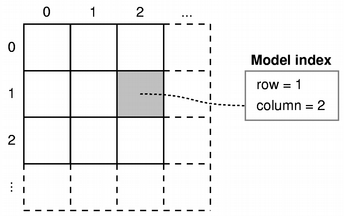
\includegraphics[width=0.5\textwidth]{modelindex-no-parent}
	\caption{model index}
\end{figure}

每个数据项都可以通过包含一个关联的模型索引的模型进行访问。
该索引可以通过 index() 函数获得。每个索引可能有一个 sibling() 索引;子项有一个 parent() 索引。

每个项目都有许多与之关联的数据元素,可以通过为模型的 data() 函数指定一个角色(请参阅 Qt::ItemDataRole)来检索它们。
可以使用 itemData() 函数同时获取所有可用角色的数据。

使用特定的 Qt::ItemDataRole 设置每个角色的数据。
可以使用 setData() 单独设置各个角色的数据,也可以使用 setItemData 设置所有角色的数据。

可以使用 flags() 查询项(请参阅 Qt::ItemFlag),以查看是否可以通过其他方式选择,拖动或操纵它们。

如果项具有子对象,则 hasChildren 为相应的索引返回 true。

该模型在层次结构的每个级别都有一个 rowCount() 和 columnCount。
可以使用 insertRows(),insertColumns(),removeRows() 和 removeColumns() 插入和删除行和列。

模型发出信号以指示变化。例如,只要模型可用的数据项发生更改,就会发出 dataChanged()。对模型提供的标题的更改将将发射 headerDataChanged() 信号。如果底层数据的结构发生了变化,则模型可以发出 layoutChanged() 来向任何附加的视图指示它们应该重新显示所显示的任何项,并需要考虑到新的结构。

可以使用 match() 函数在模型中搜索可用的项以查找特定数据。

要对模型进行排序,可以使用 sort()。

\splitLine

子类化

\begin{notice}
在模型子类化参考中有一些关于模型子类化的通用指南。
\end{notice}

子类化 QAbstractItemModel 时,至少必须实现 index(),parent(),rowCount(),columnCount() 和 data()。这些函数在所有的只读模型中使用,同样也构成了可编辑模型的基础。

还可以为模型重新实现 hasChildren() 来提供特殊的行为,而不是重新实现成本很高的 rowCount()。这使得模型可以限制视图请求的数据量,并且可以作为实现模型数据的惰性填充的一种方式。

要在模型中启用编辑,还必须实现 setData 和重新实现 flags() 以确保返回 ItemIsEditable。还可以重新实现 headerData() 和 setHeaderData 来控制呈现模型标题的方式。

当分别重新实现 setData() 和 setHeaderData() 函数时,必须显式发射 dataChanged() 和 headerDataChanged() 信号。

定制模型需要创建模型索引以供其他组件使用。为此,请使用适当的行号和列号以及相应的标识符调用 createIndex(),并将其作为指针或整数值。这些值的组合对于每个项都必须是唯一的。定制模型通常在其他重新实现的函数中使用这些唯一标识符,以检索项数据并访问有关该项的父项和子项的信息。有关唯一标识符的更多信息,请参见简单树模型示例。

不必支持 Qt::ItemDataRole 中定义的每个角色。根据模型中包含的数据类型,可能只有实现 data() 函数以返回一些更常见角色的有效信息才有用。大多数模型至少为 Qt::DisplayRole 提供项数据的文本表示,行为良好的模型也应为 Qt::ToolTipRole 和 Qt::WhatsThisRole 提供有效信息。支持这些角色可使模型与标准 Qt 视图一起使用。但是,对于某些处理高度专业化数据的模型,仅为用户定义的角色提供数据可能是合适的。

提供可调整数据结构大小的接口的模型可以提供 insertRows(),removeRows(),
insertColumns() 和 removeColumns() 的实现。在实现这些函数时,重要的是
要在模型尺寸大小发生 之前 和 之后 将有关模型尺寸的更改通知所有连接的视
图:

\begin{compactitem}
\item insertRows() 的实现必须在将新行插入数据结构 之前 调用
  beginInsertRows(),然后立即 调用 endInsertRows()。
\item insertColumns() 的实现必须在将新列插入数据结构 之前 调用
  beginInsertColumns(),然后立即 调用 endInsertColumns()。
\item removeRows() 的实现必须在从数据结构中删除行 之前 调用
  beginRemoveRows(),然后立即 调用 endRemoveRows()。
\item removeColumns() 的实现必须在列从数据结构中删除之前调用 beginRemoveColumns(),然后立即 调用 endRemoveColumns()。
\end{compactitem}

这些函数发出的私有信号使附加组件有机会在任何数据变得不可用之前采取行动。使用这些 begin 和 end 函数封装插入和删除操作还使模型能够正确地管理持久模型索引。如果希望正确处理选择,则必须确保调用了这些函数。 如果插入或移除带有子项的项,则不需要为子项调用这些函数。换句话说,父项将管理其子项。

要创建增量填充的模型,可以重新实现 fetchMore() 和 canFetchMore()。如果 fetchMore() 的重新实现向模型中添加了行,则必须调用 beginInsertRows() 和 endInsertRows()。

参见模型类、模型子类化参考、QModelIndex、QAbstractItemView、在项视图中
使用拖放、简单DOM模型示例、简单树模型示例、可编辑树模型示例和 Fetch
More示例。

\splitLine

\section{成员类型文档}

CheckIndexOption CheckIndexOptions
enum class QAbstractItemModel::CheckIndexOption flags QAbstractItemModel::CheckIndexOptions

这个枚举可以用来控制 QAbstractItemModel::checkIndex() 执行的检查。

\begin{tabular}{|m{25em}|m{4em}|m{13em}|}
\hline
常量 &值&描述\\
\hline
QAbstractItemModel::CheckIndexOption::NoOption & 0x0000	& 没有指定检查选项。\\
\hline
QAbstractItemModel::CheckIndexOption::IndexIsValid & 0x0001 & 传递给 QAbstractItemModel::checkIndex()的模型索引被检查为有效的模型索引。\\
\hline
QAbstractItemModel::CheckIndexOption::DoNotUseParent & 0x0002 & 不执行任何涉及到传递给 QAbstractItemModel::checkIndex() 的父索引的使用的检查。\\
\hline
\end{tabular}

该枚举是在 Qt 5.11 中引入或修改的。

CheckIndexOptions 类型是一个 QFlags<CheckIndexOption> 的类型定义。它存储一个或组合的 CheckIndexOption 值。

\splitLine

LayoutChangeHint

enum QAbstractItemModel::LayoutChangeHint

这个枚举描述了模型改变布局的方式。

\begin{tabular}{|l|l|l|}
\hline
常量 &值&描述\\
\hline
QAbstractItemModel::NoLayoutChangeHint&	0&	没有任何提示。\\
\hline
QAbstractItemModel::VerticalSortHint&	1&	正在对行进行排序。\\
\hline
QAbstractItemModel::HorizontalSortHint&	2&	正在对列进行排序。\\
\hline
\end{tabular}


\begin{notice}
VerticalSortHint 和 HorizontalSortHint 表示项在同一父级中移动,
而不是移动到模型中的不同父级,也没有过滤掉或过滤进来。
\end{notice}

\splitLine

\section{成员函数文档}

QAbstractItemModel

QAbstractItemModel::QAbstractItemModel(QObject *parent = nullptr)

构造指定父类对象 parent 的抽象项模型。

columnsAboutToBeInserted

[signal] void QAbstractItemModel::columnsAboutToBeInserted(const QModelIndex \&parent, int first, int last)

在将列插入模型之前就发射此信号。新项将位于给定父项 parent 下的首 first 尾 last之间。

\begin{notice}
	连接到这个信号的组件使用它来适应模型尺寸的变化。它只能由 QAbstractItemModel 的实现发射,不能在子类代码中显式发射。
\end{notice}

\begin{notice}
这是一个私有信号。它可以用于信号连接,但不能由用户发射。
\end{notice}

\begin{notice}[另请参阅]
insertColumns() 和 beginInsertColumns()。
\end{notice}

columnsAboutToBeMoved

[signal] void QAbstractItemModel::columnsAboutToBeMoved(const QModelIndex \&sourceParent, int sourceStart, int sourceEnd, const QModelIndex \&destinationParent, int destinationColumn)

模型中的列被移动之前发射该信号。将要移动的项是在给定 sourceParent 下在 sourceStart 和 sourceEnd 之间(包括首尾)的项。它们将从 destinationColumn 列开始移动到destinationParent。
 
\begin{notice}
连接到该信号的组件使用它来适应模型尺寸的变化。它只能由 QAbstractItemModel 实现发射,不能在子类代码中显式发射。
\end{notice}

\begin{notice}
这是一个私有信号。仅用于信号连接,而不能由用户发射。
\end{notice}

该函数在 Qt4.6 中被引入。

\begin{notice}[另请参阅]
beginMoveRows()。
\end{notice}

columnsAboutToBeRemoved

[signal] void QAbstractItemModel::columnsAboutToBeRemoved(const QModelIndex \&parent, int first, int last)

模型中的列被移除之前发射该信号。将要移除的项是在给定 parent 下在 first 和 last 之间(包括首尾)的项。

\begin{notice}
连接到该信号的组件使用它来适应模型尺寸的变化。它只能由 QAbstractItemModel 实现发射,不能在子类代码中显式发射。 
\end{notice}

\begin{notice}
这是一个私有信号。仅用于信号连接,而不能由用户发射。
\end{notice} 

参见 removeColumns() 和 beginRemoveColumns()。

columnsInserted

[signal] void QAbstractItemModel::columnsInserted(const QModelIndex \&parent, int first, int last)

将列插入到模型之后发射该信号。新的项是在给定 parent 下在 first 和 last 之间(包括首尾)的项。

\begin{notice}
连接到该信号的组件使用它来适应模型尺寸的变化。它只能由 QAbstractItemModel 实现发射,不能在子类代码中显式发射。
\end{notice}

\begin{notice}
这是一个私有信号。仅用于信号连接,而不能由用户发射。
\end{notice}
  
\begin{notice}[另请参阅]
insertColumns() 和 beginInsertColumns()。
\end{notice}

columnsMoved

[signal] void QAbstractItemModel::columnsMoved(const QModelIndex \&parent, int start, int end, const QModelIndex \&destination, int column)

模型中的列被移动之后发射该信号。新的项是在给定 parent 下在 start 和 end 之间(包括首尾)的项。它们将从 column 列开始移动到destination。

\begin{notice}
连接到该信号的组件使用它来适应模型尺寸的变化。它只能由 QAbstractItemModel 实现发射,不能在子类代码中显式发射。
\end{notice}

\begin{notice}
这是一个私有信号。仅用于信号连接,而不能由用户发射。
\end{notice}

该函数在 Qt4.6 中被引入。

\begin{notice}[另请参阅]
beginMoveRows()。
\end{notice}

columnsRemoved

[signal] void QAbstractItemModel::columnsRemoved(const QModelIndex \emph{\&parent}, int \emph{first}, int \emph{last})

模型中的列被移除之后发射该信号。移除的项是在给定 parent 下在 first 和 last 之间(包括首尾)的项。


\begin{notice}
连接到该信号的组件使用它来适应模型尺寸的变化。它只能由 QAbstractItemModel 实现发射,不能在子类代码中显式发射。
\end{notice}

\begin{notice}
这是一个私有信号。仅用于信号连接,而不能由用户发射。
\end{notice}

\begin{notice}[另请参阅]
removeColumns() 和 beginRemoveColumns()。
\end{notice}

dataChanged

[signal] void QAbstractItemModel::dataChanged(const QModelIndex \&topLeft, const QModelIndex \&bottomRight, const QVector<int> \&roles = QVector())

现有的项的数据发生改变时发射该信号。

如果项是同一父项,则受影响的项是在 topLeft 和 bottomRight(包含)之间的项目。如果项没有相同的父项,则行为是不确定的。

当重新实现 setData() 函数时,必须显示地发射该信号。

可选的 roles 参数可用于指定实际修改了哪些数据角色。Roles 参数中的向量为空,表示应将所有角色视为已修改。角色参数中元素的顺序没有任何关联。

\begin{notice}[另请参阅]
headerDataChanged()、setData() 和 layoutChanged()。
\end{notice}

headerDataChanged

[signal] void QAbstractItemModel::headerDataChanged(const Qt::Orientation \&orientation, int first, int last)

当标题改变时发射该信号。orientation 表示是横向标题还是竖向标题发生了改变。标题中从 first 到 last 的部分需要更新。

当重新实现 setData() 函数时,必须显示地发射该信号。

如果要更改列数或行数,则不需要发出此信号,而可以使用 begin/end 函数(有关详细信息,请参见 QAbstractItemModel 类描述中的子类化部分)。

\begin{notice}[另请参阅]
headerData()、setHeaderData() 和 dataChanged()。
\end{notice}

layoutAboutToBeChanged

[signal] void QAbstractItemModel::layoutAboutToBeChanged(const QList<QPersistentModelIndex> \&parents = QList(), QAbstractItemModel::LayoutChangeHint hint = QAbstractItemModel::NoLayoutChangeHint)

这个信号会在模型的布局改变之前发出。连接到这个信号的组件使用它来适应模型布局的变化。

在发出 layoutAboutToBeChanged() 之后,子类应该更新所有的持久化模型索引。

可选的 parents 参数用于提供更具体的通知关于模型布局的哪些部分正在被改变。空列表表示对整个模型的布局进行了更改。parents 列表中元素的顺序不重要。可选的 hint 参数用于提示模型重新布局时都发生了什么。

该函数在 Qt 5.0 中被引入。

\begin{notice}[另请参阅]
layoutChanged() 和 changePersistentIndex()。
\end{notice}

layoutChanged

[signal] void QAbstractItemModel::layoutChanged(const QList<QPersistentModelIndex> \&parents = QList(), QAbstractItemModel::LayoutChangeHint hint = QAbstractItemModel::NoLayoutChangeHint)

每当模型公开的项的布局发生变化时,就会发出这个信号,例如,对模型进行排序时。当视图接收到该信号时,应更新项的布局来反映此更改。

当对 QAbstractItemModel 或 QAbstractProxyModel 进行子类化时,请确保在更改项顺序或更改要公开给视图的数据的结构之前发出 layoutAboutToBeChanged() 信号,并在更改布局后发出 layoutChanged() 信号。

可选的 parents 参数用于给出有关模型布局的哪些部分正在更改的具体的通知。空列表表示更改了整个模型的布局。parents 列表中元素的顺序并不重要。可选的 hint 参数用于提示模型重新布局时发生的情况。

子类应在发​​出 layoutChanged() 信号之前更新所有持久模型索引。换句话说,
当结构改变时:

\begin{compactitem}
\item 发出 layoutAboutToBeChanged
\item 记住将会改变的 QModelIndex
\item 更新内部数据
\item 调用 changePersistentIndex()
\item 发出 layoutChanged
\end{compactitem}

该函数在 Qt 5.0 中被引入。

\begin{notice}[另请参阅]
layoutAboutToBeChanged()、dataChanged()、headerDataChanged()、modelReset() 和 changePersistentIndex()。
\end{notice}

modelAboutToBeReset

[signal] void QAbstractItemModel::modelAboutToBeReset()

当调用 beginResetModel() 时,在模型的内部状态(例如持久模型索引)失效之前发出这个信号。

\begin{notice}
这是一个私有信号。仅用于信号连接,而不能由用户发射。
\end{notice}

该函数在 Qt 4.2 中被引入。

\begin{notice}[另请参阅]
beginResetModel() 和 modelReset()。
\end{notice}

modelReset

[signal] void QAbstractItemModel::modelReset()

当调用 endResetModel() 时,在模型的内部状态(例如持久模型索引)失效之后发出这个信号。

注意,如果模型被重置,则应该认为之前从模型中检索的所有信息都是无效的。这包括但不限于 rowCount()、columnCount()、flags()、通过 data()检索的数据和 roleNames()。

注意: 这是一个私有信号。仅用于信号连接,而不能由用户发射。

该函数在 Qt 4.1 中被引入。

参见 endResetModel() 和 modelAboutToBeReset()。

resetInternalData

[ protected slot ] void QAbstractItemModel::resetInternalData()

该槽函数在模型的内部数据被清除并被重置之后被调用。

该槽函数为具体代理模型的子类提供了便利,例如维护了额外的数据的

QSortFilterProxyModel 的子类。

\begin{lstlisting}[language=C++]
 class CustomDataProxy : public QSortFilterProxyModel
 {
     Q_OBJECT
 public:
     CustomDataProxy(QObject *parent)
       : QSortFilterProxyModel(parent)
     {
     }

     ...

     QVariant data(const QModelIndex &index, int role) override
     {
         if (role != Qt::BackgroundRole)
             return QSortFilterProxyModel::data(index, role);

         if (m_customData.contains(index.row()))
             return m_customData.value(index.row());
         return QSortFilterProxyModel::data(index, role);
     }
 private slots:
     void resetInternalData()
     {
         m_customData.clear();
     }
 private:
   QHash<int, QVariant> m_customData;
 };
\end{lstlisting}

注意: 由于错误,该槽函数没有出现在 Qt 5.0 中。

该函数在 Qt 4.8 中被引入。

参见 modelAboutToBeReset() 和 modelReset()。

revert

[virtual slot] void QAbstractItemModel::revert()

让模型知道它应该丢弃缓存的信息。这个函数通常用于行编辑。

该函数在 Qt 4.2 中被引入。

参见 submit()。

rowsAboutToBeInserted

[ signal ] void QAbstractItemModel::rowsAboutToBeInserted(const QModelIndex \&parent, int start, int end)

在将行插入模型之前就发出该信号。新项将位于给定 parent 项目下的包含 start 和 end 之间。

注意: 连接到该信号的组件使用它来适应模型尺寸的变化。它只能由 QAbstractItemModel 实现发出,而不能在子类代码中显式发出。

注意: 这是一个私有信号。仅用于信号连接,而不能由用户发射。

参见 insertRows() 和 beginInsertRows()。

rowsAboutToBeMoved

[ signal ] void QAbstractItemModel::rowsAboutToBeMoved(const QModelIndex \&sourceParent, int sourceStart, int sourceEnd, const QModelIndex \&destinationParent, int destinationRow)

模型中的行被移动之前发射该信号。将要移动的项是在给定 sourceParent 下在 sourceStart 和 sourceEnd 之间(包括首尾)的项。它们将从 destinationRow 列开始移动到destinationParent。

注意: 连接到该信号的组件使用它来适应模型尺寸的变化。它只能由 QAbstractItemModel 实现发射,不能在子类代码中显式发射。

注意: 这是一个私有信号。仅用于信号连接,而不能由用户发射。

该函数在 Qt4.6 中被引入。

参见 beginMoveRows()。

rowsAboutToBeRemoved

[signal] void QAbstractItemModel::rowsAboutToBeRemoved(const QModelIndex \&parent, int first, int last)

模型中的行被移除之前发射该信号。将要移除的项是在给定 parent 下在 first 和 last 之间(包括首尾)的项。

注意: 连接到该信号的组件使用它来适应模型尺寸的变化。它只能由 QAbstractItemModel 实现发射,不能在子类代码中显式发射。

注意: 这是一个私有信号。仅用于信号连接,而不能由用户发射。

参见 removeRows() 和 beginRemoveRows()。

rowsInserted

[signal] void QAbstractItemModel::rowsInserted(const QModelIndex \&parent, int first, int last)

将行插入到模型之后发射该信号。新的项是在给定 parent 下在 first 和 last 之间(包括首尾)的项。

注意: 连接到该信号的组件使用它来适应模型尺寸的变化。它只能由 QAbstractItemModel 实现发射,不能在子类代码中显式发射。

注意: 这是一个私有信号。仅用于信号连接,而不能由用户发射。

参见 insertRows() 和 beginInsertRows()。

rowsMoved

[signal] void QAbstractItemModel::rowsMoved(const QModelIndex \&parent, int start, int end, const QModelIndex \&destination, int column)

模型中的行被移动之后发射该信号。新的项是在给定 parent 下在 start 和 end 之间(包括首尾)的项。它们将从 column 列开始移动到destination。

注意: 连接到该信号的组件使用它来适应模型尺寸的变化。它只能由 QAbstractItemModel 实现发射,不能在子类代码中显式发射。

注意: 这是一个私有信号。仅用于信号连接,而不能由用户发射。

该函数在 Qt4.6 中被引入。

参见 beginMoveRows()。

rowsRemoved

[signal] void QAbstractItemModel::rowsRemoved(const QModelIndex \&parent, int first, int last)

模型中的行被移除之后发射该信号。移除的项是在给定 parent 下在 first 和 last 之间(包括首尾)的项。

注意: 连接到该信号的组件使用它来适应模型尺寸的变化。它只能由 QAbstractItemModel 实现发射,不能在子类代码中显式发射。

注意: 这是一个私有信号。仅用于信号连接,而不能由用户发射。

参见 removeRows() 和 beginRemoveRows()。

submit

[virtual slot] void QAbstractItemModel::submit()

让模型知道它应该将缓存的信息提交到永久存储。这个函数通常用于行编辑。

如果没有错误,返回 true;否则返回 false。

参见 revert()。

$\sim$QAbstractItemModel

[virtual] void QAbstractItemModel::~QAbstractItemModel()

销毁抽象项模型。

beginInsertColumns

[protected] void QAbstractItemModel::beginInsertColumns(const QModelIndex \&parent, int first, int last)

开始一个列插入操作。

在子类中重新实现 insertColumns() 时,必须在将数据插入模型的底层数据存
储之前调用此函数。parent 索引对应于插入新列的父索引;first 和 last 是新
列插入后的列号。

\begin{tabular}{|m{13em}|m{26em}|}
\hline
\begin{minipage}[b]{0.3\columnwidth}
		\centering
		\raisebox{-.5\height}{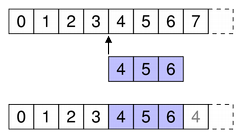
\includegraphics[width=\linewidth]{modelview-begin-insert-columns}}
\end{minipage}
&指定要插入到模型项中的列的范围的第一个和最后一个列号。例如,如图所示,我们在列4之前插入三列,所以 first 是4,last 是 6:beginInsertColumns(parent, 4, 6);这将插入三个新列作为列4、5和6。\\

\hline
%modelview-begin-append-columns.png
\begin{minipage}[b]{0.3\columnwidth}
		\centering
		\raisebox{-.5\height}{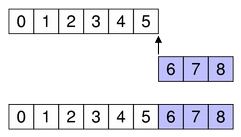
\includegraphics[width=\linewidth]{modelview-begin-append-columns}}
\end{minipage}
&
要追加列,请将它们插入到最后一列之后。例如,如图所示我们,、将三列附加到一个包含六列的集合(以列5结尾),因此 first 是 6 and last 是 8:
beginInsertColumns(parent, 6, 8);
这将追加两个新列作为列6、7和8。  \\ 
\hline
\end{tabular}

注意: 此函数发出 columnAboutToBeInserted() 信号,在插入数据之前,已连接的视图(或代理)必须处理该信号。否则,视图可能会以无效状态结束。

参见 endInsertColumns()。

\splitLine

beginInsertRows

[protected] void QAbstractItemModel::beginInsertRows(const QModelIndex \&parent, int first, int last)

开始一个行插入操作。

在子类中重新实现 insertRows() 时,必须在将数据插入模型的底层数据存储之前调用此函数。parent 索引对应于插入新列的父索引;first 和 last 是新行插入后的行号。

\begin{tabular}{|m{13em}|m{26em}|}
\hline
\begin{minipage}[b]{0.3\columnwidth}
		\centering
		\raisebox{-.5\height}{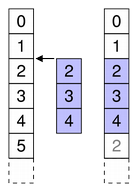
\includegraphics[width=\linewidth]{modelview-begin-insert-rows}}
\end{minipage}
&
为要插入模型中项的行范围指定第一行和最后一行。
例如,如图所示,我们在第2行之前插入三行,因此first 是2,first 是4:

beginInsertRows(parent, 2, 4);
这将插入三行新行,即第2、3和4行。
\\
\hline
%modelview-begin-append-columns.png
\begin{minipage}[b]{0.3\columnwidth}
		\centering
		\raisebox{-.5\height}{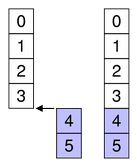
\includegraphics[width=\linewidth]{modelview-begin-append-rows}}
\end{minipage}
&
要追加行,请将它们插入到最后一行之后。例如,如图所示,我们将两行附加到一个包含4个现有行的集合(以第3行结束),因此 first 是4,last 是5:
beginInsertRows(parent, 4, 5);
这将追加两个新行作为第4行和第5行。\\ 
\hline
\end{tabular}

注意: 此函数发出 rowsAboutToBeInserted() 信号,在插入数据之前,已连接的视图(或代理)必须处理该信号。否则,视图可能会以无效状态结束。

参见 endInsertRows()。

\splitLine

beginMoveColumns

[protected] void QAbstractItemModel::beginMoveColumns(const QModelIndex \&sourceParent, int sourceFirst, int sourceLast, const QModelIndex \&destinationParent, int destinationChild)

开始一个列移动操作。

当重新实现子类时,此方法简化了模型中实体的移动。此方法负责在模型中移动持久索引,否则您将需要自己执行此操作。使用 beginMoveColumns 和 endMoveColumns() 是直接发送与 changePersistentIndex() 一起的 layoutAboutToBeChanged() 和 layoutChanged() 的另一种选择。

sourceParent 索引对应于从其移出列的父级;sourceFirst 和 sourceLast 是要移动的列的第一列和最后一列。destinationParent 索引对应于将这些列移入的父级。destinationChild 是要将列移动到的列。也就是说,sourceParent 中 sourceFirst 列的索引将成为 destinationParent 中的 destinationChild 列,然后是所有其他列,直到 sourceLast。

但是,当在同一父目录下移动列时(sourceParent 和 destinationParent 是相等的),这些列将被放置在 destinationChild 索引之前。也就是说,如果您希望移动列0和1,使它们变成列 1 和列 2,destinationChild 应该是 3。在本例中,源列 i (位于 sourceFirst 和 sourceLast 之间)的新索引等于(destinationChild-sourceLast-1+i)。

注意,如果 sourceParent 和 destinationParent 是相同的,您必须确保 destinationChild 不在 sourceFirst 和 sourceLast + 1 的范围内。还必须确保不会尝试将列移动到它自己的子列或祖先列中。如果任一条件为真,此方法将返回 false,在这种情况下,应中止移动操作。

该函数在 Qt4.6 中被引入。

参见 endMoveColumns()。

\splitLine

beginMoveRows

[protected] void QAbstractItemModel::beginMoveRows(const QModelIndex \&sourceParent, int sourceFirst, int sourceLast, const QModelIndex \&destinationParent, int destinationChild)

开始一个行移动操作。

当重新实现子类时,此方法简化了模型中实体的移动。此方法负责在模型中移动持久索引,否则您将需要自己执行此操作。使用 beginMoveRows 和 endMoveRows 是直接发送与 changePersistentIndex() 一起的 layoutAboutToBeChanged() 和 layoutChanged() 的另一种选择。

sourceParent 索引对应于从其移出行的父级;sourceFirst 和 sourceLast 是要移动的行的第一行和最后一行。destinationParent 索引对应于将这些行移入的父级。destinationChild 是要将行移动到的行。也就是说,sourceParent 中的 sourceFirst 行的索引将成为 destinationParent 中的 destinationChild 行,然后是所有其他行,直到 sourceLast。

但是,当在同一父目录下移动列时(sourceParent 和 destinationParent 是相等的),这些行将被放置在 destinationChild 索引之前。也就是说,如果您希望移动列0和1,使它们变成行 1 和行 2,destinationChild 应该是 3。在本例中,源行 i (位于 sourceFirst 和 sourceLast 之间)的新索引等于(destinationChild-sourceLast-1+i)。

注意,如果 sourceParent 和 destinationParent 是相同的,您必须确保
destinationChild 不在 sourceFirst 和 sourceLast + 1 的范围内。还必须确
保不会尝试将行移动到它自己的子列或祖先行中。如果任一条件为真,此方法将
返回 false,在这种情况下,应中止移动操作。

\begin{longtable}{|m{13em}|m{26em}|}
\hline
\begin{minipage}[b]{0.3\columnwidth}
		\centering
		\raisebox{-.5\height}{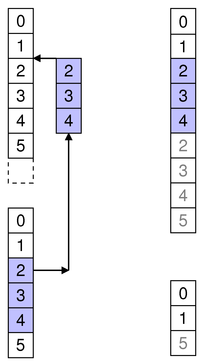
\includegraphics[width=\linewidth]{modelview-move-rows-1}}
\end{minipage}
&
指定源父行中您希望在模型中移动的行跨度的第一行和最后一行编号。还要在目
                 标父级中指定要将范围内的行移动到的行。例如,如图所示,
                 我们将源中的第 2 行到第 3 行移动了三行,因此
                 sourceFirst 为 2,sourceLast 为 4。

我们将这些项移动到目标的第2行上方,因此 destinationChild 为2。
beginMoveRows(sourceParent, 2, 4, destinationParent, 2);
这会将源中的三行第 2、3 和 4 行移动到目标中的 2、3 和 4 行。其他受影响的同级项也因此被移位。
\\
\hline
\begin{minipage}[b]{0.3\columnwidth}
		\centering
		\raisebox{-.5\height}{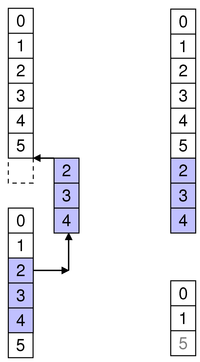
\includegraphics[width=\linewidth]{modelview-move-rows-2}}
\end{minipage}
&
若要将行追加到另一个父元素,请将它们移到最后一行的后面。例如,如图所示,我们将三行移动到一个包含 6 个现有行的集合中(以第 5 行结束),因此 destinationChild 为6:
beginMoveRows(sourceParent, 2, 4, destinationParent, 6);
这会将目标行移到目标父级的末尾,分别为 6、7 和 8。\\ 
\hline
\begin{minipage}[b]{0.3\columnwidth}
		\centering
		\raisebox{-.5\height}{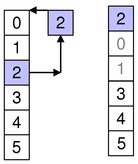
\includegraphics[width=\linewidth]{modelview-move-rows-3}}
\end{minipage}
&
要在同一父级中移动行,请指定要将其移动到的行。 例如,如图所示,我们将
                 一项从第 2 行移至第 0 行,因此 sourceFirst 和
                 sourceLast 为2,destinationChild 为0。

beginMoveRows(parent, 2, 2, parent, 0);
注意,其他行可能会相应移位。另请注意,在同一父级中移动项时,请勿尝试无效移动或无操作移动。在上面的示例中,项 2 位于移动之前的第 2 行,因此无法将其移动到第 2 行(已经存在)或第 3 行(空操作,因为第 3 行意味着已经在第 3 行之上)\\
\hline
\begin{minipage}[b]{0.3\columnwidth}
		\centering
		\raisebox{-.5\height}{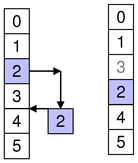
\includegraphics[width=\linewidth]{modelview-move-rows-4}}
\end{minipage}
&
要在同一父级中移动行,请指定要将其移动到的行。例如,如图所示,我们将一项从第 2 行移至第 4 行,因此 sourceFirst 和 sourceLast 为2,destinationChild 为4。
beginMoveRows(parent, 2, 2, parent, 4);
注意,其他行可能会相应移位。\\
\hline
\end{longtable}

该函数在 Qt4.6 中被引入。

参见 endMoveRows()。

beginRemoveColumns

[protected] void QAbstractItemModel::beginRemoveColumns(const QModelIndex \&parent, int first, int last)

开始一个列移除操作。

在子类中重新实现 removeColumns() 时,必须在从模型的底层数据存储中删除数据之前调用此函数。parent 索引对应于删除新列的父索引; first 和 last 是要删除的第一个和最后一个列的列号。

注意: 此函数发出 columnAboutToBeRemoved() 信号,在删除数据之前,已连接的视图(或代理)必须处理该信号。否则,视图可能会以无效状态结束。

参见 endRemoveColumns()。

\begin{tabular}{|m{13em}|m{26em}|}
\hline
\begin{minipage}[b]{0.3\columnwidth}
		\centering
		\raisebox{-.5\height}{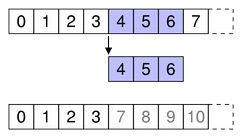
\includegraphics[width=\linewidth]{modelview-begin-remove-columns}}
\end{minipage}
&
指定要从模型中的项中删除的列的范围的第一个和最后一个列号。例如,如图所示,我们将这三列从第4列移到第6列,因此 first 是4,last 是6:
beginRemoveColumns(parent, 4, 6);\\
\hline
\end{tabular}

beginRemoveRows

[protected] void QAbstractItemModel::beginRemoveRows(const QModelIndex \&parent, int first, int last)

开始一个行移除操作。

在子类中重新实现 removeRows() 时,必须在从模型的基础数据存储中删除数据之前调用此函数。

parent 引对应于从中删除新行的父索引;first 和 last 是要删除的行的行号。

\begin{tabular}{|m{13em}|m{26em}|}
\hline
\begin{minipage}[b]{0.3\columnwidth}
		\centering
		\raisebox{-.5\height}{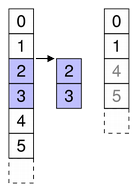
\includegraphics[width=\linewidth]{modelview-begin-remove-rows}}
\end{minipage}
&
指定要从模型中的项中删除的行范围的第一个和最后一个行号。例如,如图所示,我们将从第 2 行到第 3 行的两行删除,因此 first 是 2,last 是 3:
beginRemoveRows(parent, 2, 3);\\
\hline
\end{tabular}

%gog 
注意: 此函数发出 rowsAboutToBeRemoved() 信号,连接的视图(或代理)必须在删除数据之前处理该信号。否则,视图可能会以无效状态结束。

参见 endRemoveRows()。

beginResetModel

[protected] void QAbstractItemModel::beginResetModel()

开始模型重置操作。

重置操作会在任何附加的视图中将模型重置为当前状态。

注意: 附加到这个模型的任何视图都将被重置。

当一个模型被重置时,这意味着以前从该模型报告的任何数据现在都是无效的,必须再次进行查询。这也意味着当前项和任何选定项都将无效。当模型从根本上更改其数据时,有时只需调用此函数比在底层数据源或其结构发生更改时发出 dataChanged() 通知其他组件更容易。

在重新设置模型或代理模型中的任何内部数据结构之前,必须调用此函数。

这个函数发出信号 modelAboutToBeReset()。

该函数在 Qt4.6 中被引入。

参见 modelAboutToBeReset()、modelReset() 和 endResetModel()。

buddy

[ virtual ] void QAbstractItemModel::buddy(const QModelIndex \&index) const

返回由 index 表示的项的伙伴的模型索引。当用户想要编辑项目时,视图将调用此函数以检查是否应改为编辑模型中的另一个项。然后,视图将使用伙伴项返回的模型索引构造一个委托。

此功能的默认实现将每个项都作为自己的伙伴。

canDropMimeData

[ virtual ] bool QAbstractItemModel::canDropMimeData(const QMimeData *data, Qt::DropAction action, int row, int column, const QModelIndex \&parent) const

如果模型接受放置 data,则返回 true。这个默认实现只检查 mimeTypes() 列表中数据是否至少有一种格式,以及操作是否在模型的 supportedDropActions() 中。

如果您想要测试是否可以在 row、column、parent节点上放置 data,请在自定义模型中重新实现此函数。如果您不需要该测试,那么就没有必要重新实现此函数。

参见 dropMimeData() 和 在项视图中使用拖放。

canFetchMore

[virtual] bool QAbstractItemModel::canFetchMore(const QModelIndex \&parent) const

如果在 parent 索引下有更多可用的数据返回 true;否则返回 fasle;

默认的实现总是返回 false。

如果 canFetchMore() 返回 true,则应该调用 fetchMore() 函数。比如 QAbstractItemView 就是这样做的。

注意: 该函数可以通过元对象系统和 QML 调用。请参阅 \href{}{Q\_INVOKABLE} 。

参见 fetchMore()。

changePersistentIndex

[protected] void QAbstractItemModel::changePersistentIndex(const QModelIndex \&from, const QModelIndex \&to)

将等于给定的 from 的 QPersistentModelIndex() 模型索引更改为 to 模型索引。

如果没有找到与给定的模型索引 from 相等的持久模型索引,则什么也不会改变。

如果 canFetchMore() 返回 true,则应该调用 fetchMore() 函数。比如 QAbstractItemView 就是这样做的。

参见 persistentIndexList() 和 changePersistentIndexList()。

changePersistentIndexList

[protected] void QAbstractItemModel::changePersistentIndexList(const QModelIndexList \&from, const QModelIndexList \&to)

将等于给定的 from 的 QPersistentModelIndex()es 模型索引列表更改为 to 模型索引列表。

如果没有找到与给定的模型索引 from 相等的持久模型索引,则什么也不会改变。

该函数在 Qt4.1 中被引入。

参见 persistentIndexList() 和 changePersistentIndex()。

checkIndex

bool QAbstractItemModel::checkIndex(const QModelIndex \&index, QAbstractItemModel::CheckIndexOptions options = CheckIndexOption::NoOption) const

此函数检查索引是否为此模型的合法模型索引。 合法模型索引要么是无效的模型索引,要么是具有以下所有条件的有效模型索引:

\begin{compactitem}
\item index 的模型就是 this;
\item index 的行数大于等于零;
\item index 的行数小于父索引的行数;
\item index 的列数大于等于零;
\item index 的列数小于父索引的列数。
\end{compactitem}

options 参数可能会改变其中一些检查。如果 options 包含 IndexIsValid,那么 index 必须是一个有效的索引;这在重新实现 data() 或 setData() 等需要有效索引的函数时非常有用。

如果 options 包含 DoNotUseParent,那么将调用 parent() 的检查将被省略;允许在重新实现的 parent() 函数中调用此函数(否则,将导致无穷递归和崩溃)。

如果 options 不包含 DoNotUseParent,但包含 IndexIsValid,那么将执行额外的检查:检查父索引是否有效。这在实现平面模型(如列表或表)时非常有用,在这种情况下,模型索引不应该具有有效的父索引。

该函数如果检查成功返回 true,否则返回 false。允许在 Q\_ASSERT 和类似的其他调试机制中使用该函数。如果某些检查失败,则将在 qt.core.qabstractitemmodel.checkindex 日志记录类别中显示一条警告消息,其中包含一些可能对调试失败有用的信息。

注意: 这个函数是一个调试助手,用于实现您自己的项模型。在开发复杂模型时,以及在构建复杂的模型层次结构时(例如使用代理模型),调用这个函数来捕获传递给某个 QAbstractItemModel() API 的非法模型索引(如上定义)相关的bug是很有用的。

警告: 请注意,将非法索引传递给项模型是未定义的行为,因此应用程序必须避免这样做,并且不能依赖于项模型可以用来优雅地处理非法索引的任何“防御性”编程。

该函数在 `Qt5.11 中被引入。

参见 QModelIndex。

columnCount

[pure virtual] int QAbstractItemModel::columnCount(const QModelIndex \&parent = QModelIndex()) const

返回给定 parent 索引的子项的列的数量。

在大多数子类中,列的数量独立于 parent。

例如:

\begin{lstlisting}[language=C++]
int DomModel::columnCount(const QModelIndex &parent) const
{
     Q_UNUSED(parent);
     return 3;
}
\end{lstlisting}

% gog_c 

注意: 在实现基于表的模型时,当父模型有效时,columnCount() 应该返回 0。

注意: 该函数可以通过元对象系统和 QML 调用。请参阅 Q\_INVOKABLE。

该函数在 Qt4.1 中被引入。

参见 rowCount()。

createIndex

[protected] QModelIndex QAbstractItemModel::createIndex(int row, int column, void *ptr = nullptr) const

使用内部指针 ptr 为给定的 row 和 column 创建模型索引。

当使用 QSortFilterProxyModel 时,它的索引有自己的内部指针。不建议在模型外部访问这个内部指针。使用 data() 函数代替。

这个函数提供了一个一致的接口,模型子类必须使用这个接口来创建模型索引。

参见 QModelIndex::internalId()。

data

[pure virtual] QVariant QAbstractItemModel::data(const QModelIndex \&index, int role = Qt::DisplayRole) const

返回指定角色 role 和 索引 index 的项数据。

注意: 如果没有要返回的值,则返回无效的 QVariant,而不是返回 0。

注意: 该函数可以通过元对象系统和 QML 调用。请参阅 Q\_INVOKABLE。

参见 Qt::ItemDataRole、setData() 和 headerData()。

dropMimeData

[virtual] bool QAbstractItemModel::dropMimeData(const QMimeData *data, Qt::DropAction action, int row, int column, const QModelIndex \&parent) const

处理以给定操作 action 结束的拖放操作提供的数据 data。

如果数据和操作被模型处理了则返回 true,否则返回 false。

指定的行 row、列 column 和父索引 parent 指示模型中操作结束的项的位置。在正确的位置完成动作是模型的责任。

例如,QTreeView 中的一个项上的拖放操作可以导致新项作为行 row、列 column 和父索引 parent 指定的项的子项插入,或者作为项的兄弟项插入。

当行 row 和列 column 为 -1 时,这意味着放置的数据应该被认为是直接在 parent 上放置的。通常这意味着将数据附加为父项 parent 的子项。如果行 row 和列 column 大于或等于零,则表示放置发生在指定父索引 parent 的 row 和列 column 的前面。

调用 mimeTypes() 成员来获取可接受的 MIME 类型列表。这个默认实现假定 mimeTypes() 是默认实现,它返回一个默认 MIME 类型。如果您在自定义模型中重新实现 mimeTypes() 以返回多个 MIME 类型,那么您必须重新实现此函数以使用它们。

注意: 该函数可以通过元对象系统和 QML 调用。请参阅 Q\_INVOKABLE。

参见 supportedDropActions、canDropMimeData() 和 在项视图中使用拖放。

endInsertColumns

[protected] void QAbstractItemModel::endInsertColumns()

结束列插入操作。

在子类中重新实现 insertColumns()时,必须在将数据插入模型的底层数据存储之后调用此函数。

参见 beginInsertColumns()。

endInsertRows

[protected] void QAbstractItemModel::endInsertRows()

结束行插入操作。

在子类中重新实现 insertRows()时,必须在将数据插入模型的底层数据存储之后调用此函数。

参见 beginInsertRows()。

endMoveColumns

[protected] void QAbstractItemModel::endMoveColumns()

结束列移动操作。

在实现子类时,必须在模型的底层数据存储中移动数据之后调用此函数。

该函数在 Qt4.6 中被引入。

参见 beginMoveColumns()。

endMoveRows

[protected] void QAbstractItemModel::endMoveRows()

结束行移动操作。

在实现子类时,必须在模型的底层数据存储中移动数据之后调用此函数。

该函数在 Qt4.6 中被引入。

参见 beginMoveRows()。

endRemoveColumns

[protected] void QAbstractItemModel::endRemoveColumns()

结束列删除操作。

在子类中重新实现 removeColumns() 时,必须在从模型的底层数据存储中删除数据之后调用此函数。

参见 beginRemoveColumns()。

endRemoveRows

[protected] void QAbstractItemModel::endRemoveRows()

结束行删除操作。

在子类中重新实现 removeRows() 时,必须在从模型的底层数据存储中删除数据之后调用此函数。

参见 beginRemoveRows()。

endResetModel

[protected] void QAbstractItemModel::endResetModel()

完成模型重置操作。

在重置模型或代理模型中的任何内部数据结构后,必须调用此函数。

该函数发出 modelReset() 信号。

该函数在 Qt4.6 中被引入。

参见 beginResetModel()。

fetchMore

[ virtual ] void QAbstractItemModel::fetchMore(const QModelIndex \&parent)

获取指定的 parent 父索引的项的任何可用的数据。

如果递增地填充模型,则需要重新实现该函数。

该函数的默认实现没有做任何事情。

注意: 该函数可以通过元对象系统和 QML 调用。请参阅 Q\_INVOKABLE。

参见 canFetchMore()。

flags

[ virtual ] Qt::ItemFlags QAbstractItemModel::flags(const QModelIndex
\&index) const

返回给定索引的项标志。

基类的实现返回启用项(ItemIsEnabled)和允许选择项(ItemIsSelectable)的标志的组合。

注意: 该函数可以通过元对象系统和 QML 调用。请参阅 Q\_INVOKABLE。

参见 Qt::ItemFlags。

hasChildren

[ virtual ] Qt::ItemFlags QAbstractItemModel::hasChildren(const QModelIndex \&parent = QModelIndex()) const

如果父索引 parent 有任何子项则返回 true,否则返回 false。

在父索引上使用 rowCount() 来查找子项的数量。

注意,如果一个索引设置了 Qt::ItemNeverHasChildren 标志,那么用该索引调用该方法是未定义的行为。

注意: 该函数可以通过元对象系统和 QML 调用。请参阅 Q\_INVOKABLE。

参见 parent() 和 index()。

% gog_z 

hasIndex

[ virtual ] bool QAbstractItemModel::hasIndex(int row, int column,
const QModelIndex 
\&parent = QModelIndex()) const

如果模型返回一个指定父索引 parent、行 row 和列 column 的有效 QModelIndex,则返回 true,否则返回 false。

注意: 该函数可以通过元对象系统和 QML 调用。请参阅 Q\_INVOKABLE。

headerData

[ virtual ] QVariant QAbstractItemModel::headerData(int section, Qt::Orientation orientation, int role = Qt::DisplayRole) const

返回标题中具有给定 orientation 和 section 的数据。

对于水平标题,节号对应于列号。类似地,对于垂直标题,节号对应于行号。

注意: 该函数可以通过元对象系统和 QML 调用。请参阅 Q\_INVOKABLE。

参见 Qt::ItemDataRole、setHeaderData() 和 QHeaderView。

index

[ pure virtual ] QModelIndex QAbstractItemModel::index(int row, int column, const QModelIndex \&parent = QModelIndex()) const

返回模型中指定 row、column 和 parent 索引的项的索引。

在子类中重新实现此函数时,调用 createIndex() 来生成模型索引,其他组件可以使用这些索引来引用模型中的项。

注意: 该函数可以通过元对象系统和 QML 调用。请参阅 Q\_INVOKABLE。

参见 createIndex()。

insertColumn

bool QAbstractItemModel::insertColumn(int column, const QModelIndex \&parent = QModelIndex()) const

在指定 parent 索引的子项的指定 column 之前插入一列。

如果插入了该列,则返回 true;否则,返回 false。

注意: 该函数可以通过元对象系统和 QML 调用。请参阅 Q\_INVOKABLE。

参见 insertColumns()、insertRow() 和 removeColumn()。

insertColumns

[ virtual ] bool QAbstractItemModel::insertColumns(int column, int
count, const QModelIndex \&parent = QModelIndex()) const

在支持此功能的模型上,在模型中的给定 column 之前插入 count 列新列。每个新列中的项将是由父模型索引 parent 表示的项的子项目。

如果 column 为 0,则这些列将添加到任何现有列的前面。

如果 column 为 columnCount(),则将这些列追加到任何现有列之后。

如果 parent 没有子项,插入带有 count 列的单行。

如果列成功插入,则返回 true,否则返回 false。

基类的实现没有做任何事情,并且返回 false。

如果您实现了自己的模型,希望支持插入,则可以重新实现此函数。或者,您可以提供自己的 API 来更改数据。

注意: 该函数可以通过元对象系统和 QML 调用。请参阅 Q\_INVOKABLE。

参见 insertRows()、removeColumns()、beginInsertColumns() 和 endInsertColumns()。

insertRow

bool QAbstractItemModel::insertRow(int row, const QModelIndex \&parent = QModelIndex()) const

在指定 parent 索引的子项的指定 row 之前插入一列。

\begin{notice}
该函数调用了虚函数 insertRows()。
\end{notice}
  
如果插入了该行,则返回 true;否则,返回 false。

\begin{notice}[另请参阅]
insertRows()、insertColumn() 和 removeRow()。
\end{notice}

insertRows

[virtual] bool QAbstractItemModel::insertRows(int row, int count, const QModelIndex \&parent = QModelIndex()) const

\begin{notice}
基类的实现没有做任何事情,并且返回 false。
\end{notice}

在支持此功能的模型上,将 count 行插入模型中给定的行之前。新行中的项将是由父模型索引 parent 表示的项的子项。

如果 row 为 0,则这些行将添加到任何现有列的前面。

如果 row 为 rowCount(),则将这些列追加到任何现有行之后。

如果 parent 没有子项,插入带有 count 行的单列。

如果列成功插入,则返回 true,否则返回 false。

如果您实现了自己的模型,希望支持插入,则可以重新实现此函数。或者,您可以提供自己的 API 来更改数据。在任何一种情况下,您都需要调用 beginInsertRows() 和 endInsertRows() 来通知其他组件模型已经更改

\begin{notice}[另请参阅]
insertColumns()、removeRows()、beginInsertRows() 和 endInsertRows()。
\end{notice}

itemData

[virtual] QMap<int, QVariant> QAbstractItemModel::itemData(const QModelIndex \&index) const

为给定索引 index 处的项返回具有模型中所有预定义角色值的 map。

如果希望扩展此函数的默认行为以在 map 中包含自定义角色,请重新实现此函数。

\begin{notice}[另请参阅]
setItemData()、Qt::ItemDataRole 和 data()。
\end{notice}
  
match

[virtual] QModelIndexList QAbstractItemModel::match(const QModelIndex \&start, int role, const QVariant \&value, int hits = 1, Qt::MatchFlags flags = Qt::MatchFlags(Qt::MatchStartsWith|Qt::MatchWrap)) const

返回一列项的索引,这些索引在 start 索引的列中并且该索引下的数据在给定角色下存储的数据与指定值匹配。执行搜索的方式由给定的 flags 定义。返回的列表可能是空的。还要注意,如果使用了代理模型,列表中结果的顺序可能与模型中的顺序不一致。不能依赖结果的顺序。

搜索从 start 索引开始,直到匹配数据项的数量等于 hits,搜索到达最后一行,或者再次搜索到达start—这取决于是否在 flags 中指定了 MatchWrap。如果希望搜索所有匹配项,请使用 hits = -1。

默认情况下,此函数将对所有项执行基于字符串的包装比较,搜索以 value 指定的搜索项开头的项。 

\begin{notice}
这个函数的默认实现只搜索列。重新实现此函数以包含不同的搜索行为。
\end{notice}

\begin{notice}
该函数可以通过元对象系统和 QML 调用。
\end{notice}

\begin{notice}[另请参阅]
Q\_INVOKABLE。
\end{notice}

mimeData

[virtual] QMimeData QAbstractItemModel::mimeData(const QModelIndexList \&indexes) const

返回一个对象,该对象包含与指定索引 indexes 列表对应的序列化数据项。用于描述编码数据的格式是从 mimeTypes() 函数获得的。这个默认实现使用 mimeTypes() 的默认实现返回的默认 MIME 类型。如果您在自定义模型中重新实现 mimeTypes() 以返回更多 MIME 类型,那么重新实现此函数以使用它们。

如果 indexes 为空,或者没有受支持的 MIME 类型,则返回 0,而不是序列化的空列表。

\begin{notice}[另请参阅]
mimeTypes() 和 dropMimeData()。
\end{notice}

mimeTypes

[virtual] QStringList QAbstractItemModel::mimeTypes() const

返回允许的 MIME 类型的列表。默认情况下,内置模型和视图使用内部 MIME 类型:application / x-qabstractitemmodeldatalist。

在自定义模型中实现拖放支持时,如果您将以默认内部 MIME 类型以外的格式返回数据,请重新实现此函数以返回您的 MIME 类型列表。

如果在自定义模型中重新实现这个函数,还必须重新实现调用它的成员函数: mimeData() 和 dropMimeData()。

参见 mimeData() 和 dropMimeData()。

moveColumn

bool QAbstractItemModel::moveColumn(const QModelIndex \&sourceParent, int sourceColumn, const QModelIndex \&destinationParent, int destinationChild)

在支持此功能的模型上,将 sourceColumn从sourceParent 移到 destinationParent 下的 destinationChild。

如果列被成功移动,则返回 true;否则返回 false。

参见 moveColumns() 和 moveRow()。

moveColumns

[ virtual ] bool QAbstractItemModel::moveColumns(const QModelIndex \&sourceParent, int sourceColumn, int count, const QModelIndex \&destinationParent, int destinationChild)

在支持此功能的模型上,将 count 列从父索引 sourceParent 下的给定 sourceColumn 移到父索引 destinationParent 下的 destinationChild 列。

如果列被成功移动,则返回 true;否则返回 false。

基类的实现没有做任何事情,并且返回 false。

如果实现自己的模型,则如果要支持移动,则可以重新实现此功能。另外,您可以提供自己的 API 来更改数据。

参见 beginMoveColumns() 和 endMoveColumns()。

moveRow

bool QAbstractItemModel::moveRow(const QModelIndex \&sourceParent, int sourceRow const QModelIndex \&destinationParent, int destinationChild)

在支持此功能的模型上,将 sourceColumn从sourceParent 移到 destinationParent 下的 destinationChild。

如果行被成功移动,则返回 true;否则返回 false。

参见 moveRows() 和 moveColumn()。

moveRows

[ virtual ] bool QAbstractItemModel::moveRows(const QModelIndex \&sourceParent, int sourceRow, int count, const QModelIndex \&destinationParent, int destinationChild)

在支持此功能的模型上,将 count 行从父索引 sourceParent 下的给定 sourceColumn 移到父索引 destinationParent 下的 destinationChild 行。

如果行被成功移动,则返回 true;否则返回 false。

基类的实现没有做任何事情,并且返回 false。

如果实现自己的模型,则如果要支持移动,则可以重新实现此功能。另外,您可以提供自己的 API 来更改数据。

参见 beginMoveRows() 和 endMoveRows()。

parent

[ pure virtual ] bool QAbstractItemModel::parent(const QModelIndex \&index) const

返回具有给定索引 index 的模型项的父项。如果该项没有父项,则返回无效的 QModelIndex。

在公开树数据结构的模型中使用的常见约定是,只有第一列中的项才有子级。对于这种情况,当在子类中重新实现此函数时,返回的 QModelIndex 的列将为0。

在子类中重新实现这个函数时,要小心避免调用 QModelIndex 成员函数,比如 QModelIndex::parent(),因为模型的索引将简单地调用实现,从而导致无限递归。

\begin{notice}
该函数可以通过元对象系统和 QML 调用。
\end{notice}

\begin{notice}[另请参阅]
Q\_INVOKABLE。
\end{notice}

\begin{notice}[另请参阅]
createIndex()。
\end{notice}


persistentIndexList

[protected] QModelIndexList QAbstractItemModel::persistentIndexList() const

返回作为模型中的持久索引存储的索引列表。

该函数在 Qt4.2 中被引入。

removeColumn

bool QAbstractItemModel::removeColumn(int column, const QModelIndex \&parent = QModelIndex())

从指定的父项 parent 的子项中删除给定的列 column。

如果删除了该列,则返回 true;否则返回 false。

参见 removeColumns()、removeRow()和insertColumn()。

removeColumns

[ virtual ] bool QAbstractItemModel::removeColumns(int column, int count, const QModelIndex \&parent = QModelIndex())

在支持此功能的模型上,从模型中删除以父项 parent 下给定列 column 开头的 count 列。

如果列被成功删除,返回头 true;否则返回 false。

基类的实现没有做任何事情并返回了 false。

如果实现自己的模型,要支持删除,则可以重新实现此函数。 另外,您可以提供自己的 API 来更改数据。

参见 removeColumn()、removeRows()、insertColumns()、beginRemoveColumns() 和 endRemoveColumns()。

removeRow

bool QAbstractItemModel::removeRow(int row, const QModelIndex \&parent = QModelIndex())

从指定的父项 parent 的子项中删除给定的行 row。

如果删除了该行,则返回 true;否则返回 false。

这是一个调用 removeRows()的便利函数。QAbstractItemModel 的 removeRows()的实现不做任何事情。

参见 removeRows()、removeColumn()和insertRow()。

removeRows

[ virtual ] bool QAbstractItemModel::removeRows(int row, int count, const QModelIndex \&parent = QModelIndex())

在支持此功能的模型上,从模型中删除以父项 parent 下给定列 row 开头的 count 行。

如果行被成功删除,返回头 true;否则返回 false。

基类的实现没有做任何事情并返回了 false。

如果实现自己的模型,要支持删除,则可以重新实现此函数。 另外,您可以提供自己的 API 来更改数据。

参见 removeRow()、removeColumns()、insertColumns()、beginRemoveRows() 和 endRemoveRows()。

roleNames

[ virtual ] QHash<int, QByteArray> QAbstractItemModel::roleNames() const

返回模型的角色名称。

Qt 设置的默认角色名是:

\begin{tabular}{|l|l|}
\hline
Qt Role& QML Role Name \\ 
\hline
Qt::DisplayRole	&display\\
\hline
Qt::DecorationRole&	decoration\\
\hline
Qt::EditRole&	edit\\
\hline
Qt::ToolTipRole	&toolTip\\
\hline
Qt::StatusTipRole&	statusTip\\
\hline
Qt::WhatsThisRole&	whatsThis\\
\hline
\end{tabular}

参见 removeRow()、removeColumns()、insertColumns()、beginRemoveRows() 和 endRemoveRows()。

该函数在 Qt4.6 中被引入。

参见 setRoleNames()。

rowCount

[ pure virtual ] int QAbstractItemModel::rowCount(const QModelIndex \&parent = QModelIndex()) const

返回给定父节点 parent 下的行数。当父节点有效时,这意味着 rowCount 返回父节点的子节点数。 

\begin{notice}
在实现基于表的模型时,当父节点有效时,rowCount() 应该返回 0。
\end{notice}

\begin{notice}[另请参阅]
setSupportedDragActions()、Qt::DropActions 和 在项视图中使用拖放。
\end{notice}

\begin{notice}
该函数可以通过元对象系统和 QML 调用。
\end{notice}

\begin{notice}[另请参阅]
Q\_INVOKABLE。
\end{notice}

\begin{notice}[另请参阅]
columnCount()。
\end{notice}

setData

[virtual] bool QAbstractItemModel::setData(const QModelIndex \&index, const QVariant \&value, int role = Qt::EditRole)

将索引 index 处的项的角色数据设置为 value。

成功返回 true;否则返回 false。

如果数据被成功设置,应该发出 dataChanged() 信号。

基类的实现返回 false。对于可编辑的模型来说,该函数和 data() 必须被实现。

\begin{notice}
该函数可以通过元对象系统和 QML 调用。
\end{notice}

\begin{notice}[另请参阅]
Q\_INVOKABLE。
\end{notice}

\begin{notice}[另请参阅]
Qt::ItemDataRole、data() 和 itemData()。
\end{notice}

setHeaderData

[virtual] bool QAbstractItemModel::setHeaderData(int section, Qt::Orientation orientation, const QVariant \&value, int role = Qt::EditRole)

设置指定 section、orientation 和 role 标题的数据为 value。

标题数据更新完成,返回 true;否则返回 false。

在重新实现此函数时,必须显式发出 headerDataChanged() 信号。

\begin{notice}
该函数可以通过元对象系统和 QML 调用。
\end{notice}

\begin{notice}[另请参阅]
Q\_INVOKABLE。
\end{notice}

  
\begin{notice}[另请参阅]
Qt::ItemDataRole 和 headerData()。
\end{notice}

setItemData

[virtual] bool QAbstractItemModel::setItemData(const QModelIndex \&index, const QMap<int, QVariant> \&roles)

对于每个 Qt::ItemDataRole,将索引 index 处的项目的角色数据设置为角色中的关联值。

设置成功,返回 true;否则返回 false。

不在角色中的角色将不会被修改。

\begin{notice}[另请参阅]
setData()、data() 和 itemData()。
\end{notice}

sibling

[virtual] QModelIndex QAbstractItemModel::sibling(int row, int column, const QModelIndex \&) const

返回索引 index 项的行和列上的同级索引,如果该位置上没有同级索引,则返回无效的 QModelIndex。

sibling() 只是一个便捷函数,它找到项的父项,并使用它来检索指定行和列中子项的索引。

可以选择性地重写此方法以进行特定于实现的优化。

\begin{notice}
该函数可以通过元对象系统和 QML 调用。
\end{notice}

\begin{notice}[另请参阅]
Q\_INVOKABLE。
\end{notice}

\begin{notice}[另请参阅]
index()、QModelIndex::row() 和 QModelIndex::column()。
\end{notice}


sort

[virtual] void QAbstractItemModel::sort(int column, Qt::SortOrder order = Qt::AscendingOrder)

按给定顺序 order 按列 column 对模型进行排序。

基类实现不执行任何操作。

span

[virtual] QSize QAbstractItemModel::span(const QModelIndex \&index) const

返回由索引 index 表示的项的行和列跨度。

\begin{notice}
目前没有使用span。
\end{notice}
  

supportedDragActions

[virtual] Qt::DropActions QAbstractItemModel::supportedDragActions() const

返回此模型中数据支持的操作。

默认实现返回 supportedDropActions()。如果希望支持其他操作,请重新实现此函数。

当发生拖动时,QAbstractItemView::startDrag() 使用 supportedDragActions() 作为默认值。

\begin{notice}
目前没有使用span。
\end{notice}

\begin{notice}[另请参阅]
setSupportedDragActions()、Qt::DropActions 和 在项视图中使用拖放。
\end{notice}

supportedDropActions

[virtual] Qt::DropActions QAbstractItemModel::supportedDropActions() const

返回此模型支持的放置动作。

默认实现返回 Qt::CopyAction。如果希望支持其他操作,请重新实现此函数。您还必须重新实现 dropMimeData() 函数来处理额外的操作。

该函数在 Qt4.2 中被引入。

\begin{notice}[另请参阅]
dropMimeData()、Qt::DropActions 和 在项视图中使用拖放。
\end{notice}

%%% Local Variables:
%%% mode: latex
%%% TeX-master: "../../master"
%%% End:
\chapter{QAbstractSocket}

QAbstractSocket 类是Qt中 Socket 通信类的基类,被 QTcpSocket 和
QUdpSocket等类继承。QAbstractSocket 类为所有的socket通信类提供了最基本
的功能。

\begin{tabular}{|r|l|}
	\hline
	属性 & 方法 \\
  \hline
	头文件 & \#include<QAbstractSocket>\\      
	\hline
	qmake & QT+=network\\      
	\hline
	父类 & QIODevice\\
	\hline
	子类 & QTcpSocket、QUdpSocket \\
	\hline
\end{tabular}

\section{公共成员类型}

\begin{tabular}{|m{5em}|m{35em}|}
\hline
类型&方法 \\ 
\hline
enum&	BindFlag { ShareAddress, DontShareAddress, ReuseAddressHint,
      DefaultForPlatform }\\
\hline
flags&	BindMode\\
\hline
enum&	NetworkLayerProtocol{ IPv4Protocol, IPv6Protocol, AnyIPProtocol, UnknownNetworkLayerProtocol }\\
\hline
enum&	PauseMode { PauseNever, PauseOnSslErrors }\\
\hline
flags&	PauseModes\\
\hline
enum&	SocketError { ConnectionRefusedError, RemoteHostClosedError, HostNotFoundError, SocketAccessError, SocketResourceError, …, UnknownSocketError }\\
\hline
enum&	SocketOption{ LowDelayOption, KeepAliveOption, MulticastTtlOption, MulticastLoopbackOption, TypeOfServiceOption, …, PathMtuSocketOption }\\
\hline
enum&	SocketState { UnconnectedState, HostLookupState, ConnectingState, ConnectedState, BoundState, …, ListeningState }\\
\hline
enum&	SocketType { TcpSocket, UdpSocket, SctpSocket, UnknownSocketType }\\
  \hline
\end{tabular}

\section{公共成员函数}

\begin{longtable}{|m{15em}|m{27em}|}
\hline
类型&函数名 \\
\hline
	&QAbstractSocket(QAbstractSocket::SocketType socketType, QObject
   *parent)\\
\hline
virtual&	$\sim$QAbstractSocket()\\
\hline
void&	abort()\\
\hline
bool&	bind(const QHostAddress \&address, quint16 port = 0,
QAbstractSocket::BindMode mode = DefaultForPlatform)\\
\hline
bool&	bind(quint16 port = 0, QAbstractSocket::BindMode mode = DefaultForPlatform)\\
\hline
virtual void&	connectToHost(const QString \&hostName, quint16 port,QIODevice::OpenMode
 openMode = ReadWrite, QAbstractSocket::NetworkLayerProtocol protocol = AnyIPProtocol)\\
\hline
virtual void &connectToHost(const QHostAddress \&address, quint16 port, QIODevice::Ope
nMode openMode = ReadWrite)\\
\hline
virtual void	&disconnectFromHost()\\
\hline
QAbstractSocket::SocketError & error() const\\
\hline
bool&	flush()\\
\hline
bool&	isValid() const\\
\hline
QHostAddress&	localAddress() const\\
\hline
quint16&	localPort() const\\
\hline
QAbstractSocket::PauseModes	& pauseMode() const\\
\hline
QHostAddress&	peerAddress() const\\
\hline
QString&	peerName() const\\
\hline
quint16&	peerPort() const\\
\hline
QString&	protocolTag() const\\
\hline
QNetworkProxy&	proxy() const\\
\hline
qint64	&readBufferSize() const\\
\hline
virtual void&	resume()\\
\hline
void&	setPauseMode(QAbstractSocket::PauseModes pauseMode)\\
\hline
void&	setProtocolTag(const QString \&tag)\\
\hline
void&	setProxy(const QNetworkProxy \&networkProxy)\\
\hline
virtual void&	setReadBufferSize(qint64 size)\\
\hline
virtual bool&	setSocketDescriptor(qintptr socketDescriptor, QAbstractSocket::SocketStat
e socketState = ConnectedState, QIODevice::OpenMode openMode = ReadWrite)\\
\hline
virtual void	&setSocketOption(QAbstractSocket::SocketOption option,
const QVariant \&value)\\
\hline
virtual qintptr&	socketDescriptor() const\\
\hline
virtual QVariant&	socketOption(QAbstractSocket::SocketOption option)\\
\hline
QAbstractSocket::SocketType	&socketType() const\\
\hline
QAbstractSocket::SocketState&	state() const\\
\hline
virtual bool&	waitForConnected(int msecs = 30000)\\
\hline
virtual bool&	waitForDisconnected(int msecs = 30000)\\
\hline
\end{longtable}

\section{重载公共成员函数}

\begin{tabular}{|l|l|}
\hline
类型& 函数名\\ 
\hline
virtual bool&atEnd() const override\\
\hline
virtual qint64&	bytesAvailable() const override\\
\hline
virtual qint64&		bytesToWrite() const override\\
\hline
virtual bool&	canReadLine() const override\\
\hline
virtual void&	close() override\\
\hline
virtual bool&	isSequential() const override\\
\hline
virtual bool&	waitForBytesWritten(int msecs = 30000) override\\
\hline
virtual bool&	waitForReadyRead(int msecs = 30000) override\\
\hline
\end{tabular}

\section{信号}

\begin{tabular}{|m{5em}|m{35em}|}
\hline
类型&函数名 \\
\hline
void&	connected()\\
\hline
void&	disconnected()\\
\hline
void&	errorOccurred(QAbstractSocket::SocketError socketError)\\
\hline
void&	hostFound()\\
\hline
void&	proxyAuthenticationRequired(const QNetworkProxy \&proxy,
                                                          QAuthenticator
                                                          *authenticator)\\
\hline
void&	stateChanged(QAbstractSocket::SocketState socketState)\\
\hline
\end{tabular}

\section{保护成员函数}

\begin{tabular}{|m{5em}|m{35em}|}
\hline
类型&函数名 \\
\hline
void&	setLocalAddress(const QHostAddress \&address)\\
\hline
void&	setLocalPort(quint16 port)\\
\hline
void&	setPeerAddress(const QHostAddress \&address)\\
\hline
void&	setPeerName(const QString \&name)\\
\hline
void&	setPeerPort(quint16 port)\\
\hline
void&	setSocketError(QAbstractSocket::SocketError socketError)\\
\hline
void&	setSocketState(QAbstractSocket::SocketState state)\\
\hline
\end{tabular}

重载保护成员函数

\begin{tabular}{|m{5em}|m{35em}|}
\hline
类型&函数名 \\
\hline
virtual qint64&	readData(char *data, qint64 maxSize) override\\
\hline
virtual qint64&	readLineData(char *data, qint64 maxlen) override\\
\hline
virtual qint64&	writeData(const char *data, qint64 size) override\\
\hline
\end{tabular}

\section{详细介绍}

QAbstractSocket 类是 QTcpSocket 类和 QUdpSocket 类的基类,包含了这两个
类所有的常规功能。您可以通过以下两种方法使用一个套接字( Socket ):

\begin{compactitem}
\item 实例化一个 QTcpSocket 或者 QUdpSocket 对象
\item 声明一个自定义套接字描述符,实例化 QAbstractSocket ,然后调用 setSocketDescriptor() 函数包装该自定义套接字描述符。
\end{compactitem}

TCP(传输控制协议)是一种可靠的,面向流,面向连接的传输协议。 UDP(用户数据报协议)是一种不可靠的,面向数据报的无连接协议。 实际上,这意味着TCP更适合于连续数据传输,而当可靠性不重要时,可以使用更轻量的UDP。

QAbstractSocket 的 API 统一了这两种协议之间的大部分差异。 例如,尽管 UDP 是无连接的,但 connectToHost() 为 UDP 套接字建立了虚拟连接,使您可以忽略底层协议,以几乎相同的方式使用 QAbstractSocket 类。 在 QAbstractSocket 类的内部实现中,QAbstractSocket 记录了传递给 connectToHost() 的地址和端口,并且能在调用 read() 和 write() 之类的成员函数时使用这些值。

任何情况下,QAbstractSocket 类都有一个状态( state ,该值可以由 state() 成员函数的返回值获得)。 初始状态为未连接( QAbstractSocket :: UnconnectedState )状态。 调用 connectToHost() 成员函数连接主机后,套接字会首先进入寻找主机( QAbstractSocket :: HostLookupState )状态。 如果找到了主机,则 QAbstractSocket 会进入连接中( QAbstractSocket :: ConnectingState )状态,并发送 hostFound() 信号。 建立连接后,它将进入已连接( QAbstractSocket :: ConnectedState )状态并发送 connected() 信号。 如果在以上列出任何阶段发生了错误,则会发出 errorOccurred() 信号。 每当状态发生更改时,QAbstractSocket 都会发出 stateChanged() 信号。 为方便起见,当套接字已准备好进行读取和写入数据操作时,isValid() 成员函数的返回值为 true 。但是要注意一下,在进行读写操作之前,套接字的状态必须为已连接( QAbstractSocket :: ConnectedState )状态。

您可以通过调用 read() 或 write() 来进行数据读写操作,同时为了方便进行特殊的数据读入操作,您还可以使用 QAbstractSocket 的父类 QIODevice 提供的成员函数 readLine() 和 readAll() 。当我们需要以字节为单位进行数据读写操作时,可以使用 QAbstractSocket 的父类 QIODevice 提供的成员函数 getChar(),putChar() 和 ungetChar() 。 待数据写入套接字后,QAbstractSocket 会发出继承自父类 QIODevice 的信号 bytesWritten() 。请特别注意一下,Qt并不限制写缓冲区的大小。 您可以通过监听 bytesWritten() 信号来监视其大小。

每当有新的数据块到达时,QAbstractSocket 都会发出继承自父类 QIODevice 的信号 readyRead() 。 您可以通过 bytesAvailable() 成员函数的返回值来获得当前读取缓冲区中可读取的字节数。 通常来讲,您可以将 readyRead() 信号与一个槽函数相连接,然后在该槽函数中读取所有可用的数据。 如果您不一次性读取所有数据,则其余数据以后仍可以读取,并且任何新的传入数据都将追加到 QAbstractSocket 的内部读取缓冲区中。您可以通过调用 setReadBufferSize() 成员函数来限制读取缓冲区的大小。

您可以通过调用 disconnectFromHost() 成员函数关闭套接字。 调用 disconnectFromHost() 成员函数后,QAbstractSocket 会进入关闭中( QAbstractSocket :: ClosingState )状态。 待所有未处理数据写入套接字后,QAbstractSocket 将关闭套接字,进入未连接( QAbstractSocket :: UnconnectedState )状态,并发送 disconnected() 信号。 如果要立即中止连接,并丢弃所有未处理数据,请调用 abort() 成员函数。 如果远程主机关闭了该连接,QAbstractSocket 将发出 errorOccurred(QAbstractSocket :: RemoteHostClosedError) 错误信号,在此期间套接字状态仍为已连接( QAbstractSocket :: ConnectedState )状态,此后将发送 disconnected() 信号。

您可以通过调用 peerPort() 和 peerAddress() 成员函数来获取已连接的对等方的端口和地址。 peerName() 成员函数则会返回传递给 connectToHost() 的对等方的主机名。 另外,localPort() 和 localAddress() 成员函数可返回本地套接字的端口和地址。

QAbstractSocket 提供了一组函数,这些函数可以挂起调用线程,直到发出某些
信号为止。 这些函数可用于实现阻塞套接字:

\begin{compactitem}
\item waitForConnected() 阻塞套接字直到一个新的连接建立
\item waitForReadyRead() 阻塞套接字直到有新的数据可以读取
\item waitForBytesWritten() 阻塞套接字直到一个有效的荷载数据写入到了套接字
\item waitForDisconnected() 阻塞套接字直到连接已经关闭
\end{compactitem}



Qt官方提供了如下示例:

\begin{lstlisting}[language=C++]
int numRead = 0, numReadTotal = 0;
char buffer[50];

forever {
	numRead  = socket.read(buffer, 50);

	// do whatever with array

	numReadTotal += numRead;
	if (numRead == 0 && !socket.waitForReadyRead())
		break;
}

\end{lstlisting}

waitForReadyRead() 成员函数返回值为 false,则说明连接已关闭或发生了错误。

使用阻塞套接字进行编程与使用非阻塞套接字进行编程完全不同。 阻塞套接字不需要有一个事件循环,这通常可以简化代码。 但是,在GUI应用程序中,阻塞套接字只能在非GUI线程中使用,以避免冻结用户界面。 有关这两种方法的概述,请参见 fortuneclien 和 blockingfortuneclient 示例。

\begin{notice}
Qt官方并不推荐将阻塞函数与信号一起使用。
\end{notice}


QAbstractSocket 可以与 QTextStream 和 QDataStream 的流运算符(operator<<() 和operator>>())一起使用。 但是,有一个问题需要注意:在尝试使用operator>>() 读取数据之前,必须确保有足够的数据可用。

\begin{notice}[另请查阅]
QNetworkAccessManager 类和 QTcpServer。
\end{notice}

\splitLine

成员类型文档

enum QAbstractSocket::BindFlag | flags QAbstractSocket::BindMode
该枚举描述了一些不同的标志,这些标志可以传递为 bind() 成员函数的参数,指定了不同的主机绑定模式。

\begin{tabular}{|m{10em}|m{5em}|m{30em}|}
\hline
常量&值&描述 \\
\hline
QAbstractSocket::ShareAddress&	0x1	&允许其他服务绑定到相同的地址和端口。
                               在多个进程通过侦听相同的地址和端口来分
                               担单个服务的负载的情况下(例如,具有多
                               个预分支侦听器的Web服务器可以大大缩短响
                               应时间),该模式十分有效。 但是,由于该
                               模式下允许任何服务对主机进行重新绑定,
                               因此此选项存在着安全隐患。 请注意,您还
                               可以允许您的服务重新绑定现有的共享地址
                               通过将此选项与
                               QAbstractSocket::ReuseAddressHint 结合
                               使用。 在 Unix 上,这等效于
                               SO\_REUSEADDR 套接字选项。 在 Windows 上,
                               这是默认行为,因此将忽略此选项。\\
\hline
QAbstractSocket::DontShareAddress&	0x2&	绑定主机时独占地址和端口,不允
                                   许其他服务重新绑定。 将此选项作为
                                   QAbstractSocket :: bind() 参数,可
                                   以确保在绑定主机成功后,您当前的服
                                   务是唯一侦听指定地址和端口的服务。
                                   即使其他服务通过指定
                                   QAbstractSocket::ReuseAddressHint
                                   模式来绑定服务,这个操作也是不允许
                                   的。 该模式相比
                                   QAbstractSocket::ShareAddress 提供
                                   了更高的安全性,但是在某些操作系统
                                   上,它要求您以管理员权限运行该服务。
                                   在 Unix 和 macOS 上,独占地址和端口
                                   是绑定主机的默认行为,因此该选项将
                                   被忽略。 在 Windows 上,此选项使用
                                   SO\_EXCLUSIVEADDRUSE 套接字选项。\\
\hline
QAbstractSocket::ReuseAddressHint&	0x4	&示意 QAbstractSocket 即使地址
                                   和端口已被另一个套接字绑定,它也应
                                   尝试重新绑定服务。 在 Windows 和
                                   Unix 上,这等效于 SO\_REUSEADDR 套接
                                   字选项。\\
\hline
QAbstractSocket::DefaultForPlatform&	0x0&	使用当前平台的默认模式。 在 Unix 和 macOS 上,这等效于( QAbstractSocket::DontShareAddress + QAbstractSocket::ReuseAddressHint ),在 Windows 上,它等效于 QAbstractSocket::ShareAddress 。\\
\hline
\end{tabular}

该枚举最初在Qt5.0版本引入。

BindMode 类型是 typedef QFlags <BindFlag> 生成的用户自定义类型。 它存储着 BindFlag 值的 OR 组合。

enum QAbstractSocket::NetworkLayerProtocol

该枚举描述了Qt中可以使用的网络层协议

\begin{tabular}{|m{26em}|m{2em}|m{8em}|}
\hline
常量&值&描述 \\
\hline
QAbstractSocket::IPv4Protocol&	0	&IPv4\\
\hline
QAbstractSocket::IPv6Protocol&	1	&IPv6\\
\hline
QAbstractSocket::AnyIPProtocol&	2	&IPv4 或 IPv6\\
\hline
QAbstractSocket::UnknownNetworkLayerProtocol&	-1	&除IPv4和IPv6之外的协议\\
\hline
\end{tabular}

您也可以在 QHostAddress::protocol() 中找到有关网络层协议的相关知识。

enum QAbstractSocket::PauseMode | flags QAbstractSocket::PauseModes

该枚举描述了套接字在什么情况下该停止传输中的数据。 

当前Qt支持的唯一通知是 QSslSocket::sslErrors()。

\begin{tabular}{|m{19em}|m{2em}|m{18em}|}
%\begin{tabular}{|C{.15\textwidth}|C{.5\textwidth}|C{.15\textwidth}|}}
\hline
常量	&值&	描述\\
\hline
QAbstractSocket::PauseNever&	0x0&	“永远”不暂停套接字上的数据传输。 该模
  式是默认设置,符合Qt 4的标准。\\
\hline
QAbstractSocket::PauseOnSslErrors&	0x1&	收到 SSL 错误(即 QSslSocket::sslErrors() )的通知后,暂停套接字上的数据传输。\\
\hline
\end{tabular}

该枚举最初在Qt5.0版本引入。

PauseModes 类型是 typedef QFlags<PauseMode> 生成的用户自定义类型。它储存着 PauseMode 值的 OR 组合。

enum QAbstractSocket::SocketError

该枚举描述了常见的套接字错误。

\begin{longtable}{|m{20em}|m{2em}|m{19em}|}
\hline
常量&	值&	描述 \\ 
\hline
QAbstractSocket::ConnectionRefusedError&	0&	连接被对方拒绝(或连接超时)。\\
\hline
QAbstractSocket::RemoteHostClosedError&	1&	远程主机关闭了连接。 请注意,在发送远程
主机连接关闭的通知后,客户端套接字(即此套接字)将被关闭。\\
\hline
QAbstractSocket::HostNotFoundError&	2&	未能找到主机地址。\\
\hline
QAbstractSocket::SocketAccessError&	3&	程序没有权限来进行特定的套接字操作\\
\hline
QAbstractSocket::SocketResourceError&	4&	本地系统资源不足(例如本地系统使用了过多的套接字)。\\
\hline
QAbstractSocket::SocketTimeoutError&	5&	套接字操作超时。\\
\hline
QAbstractSocket::DatagramTooLargeError&	6&	数据报大于操作系统的限制(该限制可以低至
8192字节)。\\
\hline
QAbstractSocket::NetworkError&	7&	网络发生错误(例如网线断开)。\\
\hline
QAbstractSocket::AddressInUseError&	8&	QAbstractSocket::bind() 指定的主机地址已
被另一个套接字使用独占模式绑定。\\
\hline
QAbstractSocket::SocketAddressNotAvailableError&	9& QAbstractSocket::bind() 指定的主机地址不属于主机。\\
\hline
QAbstractSocket::UnsupportedSocketOperationError&	10&	本地操作系统不支持请求的套
接字操作(例如,缺少IPv6支持)。\\
\hline
QAbstractSocket::ProxyAuthenticationRequiredError&	12&	套接字正在使用代理,并且代
理需要身份验证。\\
\hline
QAbstractSocket::SslHandshakeFailedError&	13&	SSL / TLS 握手失败,因此连接已关
闭(仅在 QSslSocket 中使用)。\\
\hline
QAbstractSocket::UnfinishedSocketOperationError&	11&	仅由QAbstractSocketEngine 使用,上一次尝试的操作尚未完成(仍在后台进行)。\\
\hline
QAbstractSocket::ProxyConnectionRefusedError&	14&	代理服务器拒绝了连接。\\
\hline
QAbstractSocket::ProxyConnectionClosedError&	15&	与代理服务器的连接意外关闭(在
建立与对方的最终连接之前)。\\
\hline
QAbstractSocket::ProxyConnectionTimeoutError&	16&	与代理服务器的连接超时或代理服
务器在身份验证阶段停止响应。\\
\hline
QAbstractSocket::ProxyNotFoundError&	17&	找不到使用 setProxy() (或应用程序代理
)设置的代理地址。\\
\hline
QAbstractSocket::ProxyProtocolError&	18&	与代理服务器通信失败,因为无法理解来自代
理服务器的响应,这通常是代理服务协议错误的锅。\\
\hline
QAbstractSocket::OperationError&	19&	套接字所处的状态不允许该操作\\
\hline
QAbstractSocket::SslInternalError&	20&	使用的 SSL 库出现内部错误。 这可能是由于 SS
L 库安装错误或配置错误造成的。\\
\hline
QAbstractSocket::SslInvalidUserDataError&	21&	提供了无效的数据(证书,密钥,密码
等),其使用导致 SSL 库出现错误。\\
\hline
QAbstractSocket::TemporaryError&	22&	发生临时错误(例如,操作将阻塞套接字,而套接
字未阻塞)。\\
\hline
QAbstractSocket::UnknownSocketError&	-1&	神了,出现了一个未知错误。\\
\hline
\end{longtable}

\begin{notice}[另请查阅]
QAbstractSocket::error() 和 QAbstractSocket::errorOccurred()。
\end{notice}


\splitLine

enum QAbstractSocket::SocketOption

该枚举表示可以在套接字上设置的选项。 如果需要设置这些选项,您可以在套接字接收到 connectd() 信号之后,或者在 QTcpServer 接收到新的套接字之后,对它们进行设置。

\begin{tabular}{|l|l|l|}
\hline
常量&	值&	描述 \\ 
\hline
QAbstractSocket::LowDelayOption&	0&	尝试优化套接字以降低延迟。 对
                                       于 QTcpSocket ,这将设置
                                       TCP\_NODELAY 选项并禁用 Nagle 的
                                       算法。 将此设置为1启用。\\
\hline
QAbstractSocket::KeepAliveOption&	1&	将此设置为1以启用 SO\_KEEPALIVE 套接字选项\\
\hline
QAbstractSocket::MulticastTtlOption&	2&	将此设置为整数值以设置
                                           IP\_MULTICAST\_TTL (多播数据
                                           报的 TTL )套接字选项。\\
\hline
QAbstractSocket::MulticastLoopbackOption&	3&	将此设置为1以启用
                                               IP\_MULTICAST\_LOOP (多
                                               播环回)套接字选项。\\
\hline
QAbstractSocket::TypeOfServiceOption&	4&	Windows 不支持此选项。 这
                                           映射到IP\_TOS套接字选项。 有
                                           关其可能的可取值,请参见下
                                           表。\\
\hline
QAbstractSocket::SendBufferSizeSocketOption&	5&	在操作系统级别设置
                                                   套接字发送缓冲区的
                                                   大小(以字节为单位)。
                                                   这映射到 SO\_SNDBUF
                                                   套接字选项。 该选项
                                                   不会影响 QIODevice
                                                   或 QAbstractSocket
                                                   缓冲区。 这个枚举值
                                                   在Qt 5.3中引入。\\
\hline
QAbstractSocket::ReceiveBufferSizeSocketOption&	6&	在操作系统级别设置
                                                   套接字接收缓冲区的
                                                   大小(以字节为单位)。
                                                   这映射到 SO\_RCVBUF
                                                   套接字选项。 此选项
                                                   不会影响 QIODevice
                                                   或 QAbstractSocket
                                                   缓冲区(请参见
                                                   setReadBufferSize()
                                                   )。 这个枚举值已在
                                                   Qt 5.3中引入。\\
\hline
QAbstractSocket::PathMtuSocketOption&	7	&检索IP堆栈当前已知的路径最大传输单位( PMTU )值(如果该值存在)。 一些IP堆栈还允许设置 MTU 进行传输。 这个枚举值在Qt 5.11中引入。\\
\hline
\end{tabular}

TypeOfServiceOption 可能的可取值(优先级):

\begin{tabular}{|l|l|}
\hline
值&	描述 \\
\hline
224&	Network control(网络控制)\\
\hline
192&	Internetwork control(互联网络控制)\\
\hline
160&	CRITIC/ECP(至关重要)\\
\hline
128&	Flash override(火速覆盖)\\
\hline
96&	Flash(火速)\\
\hline
64&	Immediate(立即)\\
\hline
32&	Priority(主要)\\
\hline
0&	Routine(常规) \\
\hline
\end{tabular}

该枚举最初在Qt4.6版本引入。

\begin{notice}[另请查阅]
QAbstractSocket::setSocketOption() 和 QAbstractSocket::socketOption()。
\end{notice}


\splitLine

enum QAbstractSocket::SocketState
该枚举描述了套接字不同的状态。

\begin{tabular}{|l|l|l|}
\hline
常量&	值&	描述 \\ 
\hline
QAbstractSocket::UnconnectedState&	0&	套接字未连接。\\
\hline
QAbstractSocket::HostLookupState&	1&	套接字正在查询主机。\\
\hline
QAbstractSocket::ConnectingState&	2&	套接字开始建立连接。\\
\hline
QAbstractSocket::ConnectedState&	3&	新的连接已建立。\\
\hline
QAbstractSocket::BoundState&	4&	套接字已绑定到一个地址和端口。\\
\hline
QAbstractSocket::ClosingState&	6&	套接字即将关闭(数据可能仍在等待写入)。\\
\hline
QAbstractSocket::ListeningState&	5&	套接字仅限内部使用。\\
\hline
\end{tabular}


\begin{notice}[另请查阅]
QAbstractSocket::state()。
\end{notice}

\splitLine

enum QAbstractSocket::SocketType

该枚举描述了传输层的协议。

\begin{tabular}{|l|l|l|}
\hline
常量&	值&	描述 \\ 
\hline
QAbstractSocket::TcpSocket&	0&	TCP \\ 
\hline
QAbstractSocket::UdpSocket&	1&	UDP\\ 
\hline
QAbstractSocket::SctpSocket&	2&	SCTP\\
\hline
QAbstractSocket::UnknownSocketType&	-1&	除 TCP, UDP 和 SCTP 外的协议\\
\hline
\end{tabular}



\begin{notice}[另请查阅]
QAbstractSocket::socketType() 。
\end{notice}

\splitLine


\section{成员函数文档}

QAbstractSocket::QAbstractSocket(QAbstractSocket::SocketType
socketType, QObject *parent)

创建一个新抽象套接字 socketType 。 函数中父对象的参数传递给 QObject 的构造函数。

这就是它的构造函数嘛,没啥好说的。另外由于 QAbstractSocket 类继承自 QObject 类,应注意在 QAbstractSocket 类构造函数中调用一下父类 QObject 类的构造函数。


\begin{notice}[另请查阅]
socketType() 、 QTcpSocket 和 QUdpSocket 。
\end{notice}


[SIGNAL] void QAbstractSocket::connected()

connectToHost() 调用并成功建立一个连接后,QAbstractSocket 类将发送 connectd() 信号。


\begin{notice}
在某些操作系统上,connected() 信号可能直接从 connectToHost() 调用发出,以连接到本地主机。
\end{notice}


\begin{notice}[另请查阅]
connectToHost() 和 disconnected()。
\end{notice}



[SIGNAL] void QAbstractSocket::disconnected()

套接字断开后会发送该信号。

\begin{notice}[警告]
如果您想在与这个信号相连接的槽函数中删除信号的发送者( sender() ),请使用 deleteLater() 函数。
\end{notice}


\begin{notice}[另请查阅]
connectToHost() 、disconnectFromHost() 和 abort()。
\end{notice}



[SIGNAL] void
QAbstractSocket::errorOccurred(QAbstractSocket::SocketError
socketError)

当套接字遇到错误时会发送该信号。socketError 参数描述了该错误类型。

发出此信号后,套接字可能并未准备好进行重新连接。 在这种情况下,我们应尝试从事件循环中进行重新连接。 例如我们可以调用一个QTimer::singleShot(),并将0作为时间间隔。

请注意,QAbstractSocket :: SocketError 并不是Qt预注册好的元类型。因此如果您要在队列连接( queued connections )模式的信号与槽的连接中传递该类型的参数,您必须使用 Q\_DECLARE\_METATYPE() 和 qRegisterMetaType() 注册它为元类型。

该函数在Qt5.15版本引入。


\begin{notice}[另请查阅]
error()、 errorString() 和 Creating Custom Qt Types。
\end{notice}


[SIGNAL] void QAbstractSocket::hostFound()

在 QAbstractSocket 调用 connectToHost() 函数并成功找到主机后,它将发送该消息。

\begin{notice}
从Qt 4.6.3开始,由于可能已缓存DNS结果,因此 QAbstractSocket 可能直接在调用 connectToHost() 时发送 hostFound() 信号。
\end{notice}



\begin{notice}[另请查阅]
connectd()。
\end{notice}

[SIGNAL] void QAbstractSocket::proxyAuthenticationRequired(const
QNetworkProxy \&proxy, QAuthenticator *authenticator)

套接字连接的代理服务期需要身份验证时会发送该消息。您可以用所需的详细信息填充 authenticator 对象,以便代理服务期进行身份验证并继续连接。


\begin{notice}
如果信号返回时未使用新信息填充 authenticator ,则连接将失败,因此您不能使用队列连接模式( QueuedConnection )连接到该信号。
\end{notice}


该函数首次在Qt4.3版本引入。

\begin{notice}[另请查阅]
QAuthenticator 和 QNetworkProxy。
\end{notice}

[SIGNAL] void
QAbstractSocket::stateChanged(QAbstractSocket::SocketState
socketState)

QAbstractSocket 状态发生改变后会发送该信号。socketState 参数记录了新的状态。

\begin{notice}
QAbstractSocket::SocketState 并不是Qt预注册好的元类型。因此如果您要在队列连接( queued connections )模式的信号与槽的连接中传递该类型的参数,您必须使用 Q\_DECLARE\_METATYPE() 和 qRegisterMetaType() 注册它为元类型。
\end{notice}


\begin{notice}[另请查阅]
state() 和 Create Custom Qt Types 。
\end{notice}


[virtual] QAbstractSocket::$\sim$QAbstractSocket()

析构函数,销毁套接字。

void QAbstractSocket::abort()

中止当前连接并重置套接字。 与 disconnectFromHost() 不同,此函数会立即关闭套接字,并丢弃写缓冲区中的所有未处理数据。



\begin{notice}[另请查阅]
 disconnectFromHost() 和 close() 。
\end{notice}



[override virtual] bool QAbstractSocket::atEnd() const

该函数重写了父类 QIODevice 的类成员函数 QIODevice::atEnd() const 。

如果当前没有更多数据可读取,则返回 true ,否则返回 false 。

在循环中从套接字读取数据时,最常使用此功能。 例如:

\begin{lstlisting}[language=C++]
// This slot is connected to QAbstractSocket::readyRead()
void SocketClass::readyReadSlot()
{
	while (!socket.atEnd()) {
		QByteArray data = socket.read(100);
		....
	}
}
\end{lstlisting}



\begin{notice}[另请查阅]
bytesAvailable() 和 readyRead() 。
\end{notice}


\splitLine

bool QAbstractSocket::bind(const QHostAddress \&address, quint16] port
= 0, QAbstractSocket::BindMode mode = DefaultForPlatform)

使用 mode 指定的 QAbstractSocket::BindMode 模式绑定到 address 和 port 指定的地址和端口上。

对于 UDP 套接字来说,在使用 bind() 绑定主机后,只要 UDP 数据报到了达指定的地址和端口,就会发出 QUdpSocket :: readyRead() 的信号。 因此,此功能对于编写UDP服务器很有用。

对于 TCP 套接字来说,此功能可用于指定将哪个接口用于传出连接,这在多个网络接口的情况下很有用。

默认情况下, QAbstractSocket 会使用 DefaultForPlatform BindMode 模式绑定套接字。 如果未指定端口 port ,则 QAbstractSocket 会选择一个随机端口。

成功后,函数返回 true ,套接字进入 已绑定 ( BoundState )状态; 否则返回 false 。

该函数最初在Qt5.0版本引入。

bool QAbstractSocket::bind(quint16 port = 0, QAbstractSocket::BindMode
mode = DefaultForPlatform)

重载 bind() 函数。

该函数会使用 mode 指定的 QAbstractSocket::BindMode 模式绑定到主机上的任何地址( QHostAddress:Any ) 和 port 指定的端口上。

默认情况下, QAbstractSocket 会使用 DefaultForPlatform BindMode 模式绑定套接字。 如果未指定端口 port ,则 QAbstractSocket 会选择一个随机端口。

该函数最初在Qt5.0版本引入。

[override virtual] qint64 QAbstractSocket::bytesAvailable() const

该函数重写了父类 QIODevice 的类成员函数 QIODevice::bytesAvailable() const 。

返回等待读取的传入字节数。


\begin{notice}[另请查阅]
bytesToWrite() 和 read() 。
\end{notice}

[override virtual] qint64 QAbstractSocket::bytesToWrite() const

该函数重写了父类 QIODevice 的类成员函数 QIODevice::bytesToWrite() const 。

返回等待写入的字节数。 当控制权返回事件循环或调用 flush() 时,这些字节将会被写入。



\begin{notice}[另请查阅]
 bytesAvailable() 和 flush() 。
\end{notice}

[override virtual] bool QAbstractSocket::canReadLine() const

该函数重写了父类 QIODevice 的类成员函数 QIODevice::canReadLine() const 。

如果能从该套接字中读取一行数据时返回 true,否则返回 false 。



\begin{notice}[另请查阅]
readLine() 。
\end{notice}

[override virtual] void QAbstractSocket::close()

该函数重写了父类 QIODevice 的类成员函数 QIODevice::close() 。

关闭套接字的 I/O 设备并调用 disconnectFromHost() 来关闭套接字的连接。

您可以阅读 QIODevice::close() 的介绍来查阅关闭 I/O 设备时发生的操作。


\begin{notice}[另请查阅]
abort() 。
\end{notice}


[virtual] void QAbstractSocket::connectToHost(const QString \&hostName,
quint16 port, QIODevice::OpenMode openMode = ReadWrite,
QAbstractSocket::NetworkLayerProtocol protocol = AnyIPProtocol)

尝试连接到远程主机 hostname 的给定端口 port 。 protocol 参数可用于指定要使用的网络协议(例如IPv4或IPv6)。

使用 openMode 给定的模式打开套接字并进入 寻找主机( HostLookupState )状态,然后 QAbstractSocket 开始执行主机名查找操作。 成功查找到主机名后, QAbstractSocket 会发出 hostFound() 信号,并进入连接中( ConnectingState )状态。 接着 QAbstractSocket 会尝试连接到上一部查找主机后返回的一个或多个地址。 最终建立连接后,QAbstractSocket 会进入已连接 ( ConnectedState )并发送 connectd() 信号。

在以上的任意一阶段中遇到错误,套接字都会发送 errorOccurred() 信号。

hostName 参数可以是一个字符串形式的IP地址(例如"49.195.83.32"),也可以是一个主机名(例如"example.com")。QAbstractSocket 仅在需要时才会进行查找。 port 端口参数按本机字节顺序。


\begin{notice}[另请查阅]
state()、peerName()、peerAddress()、peerPort() 和 waitForConnected()。
\end{notice}


[virtual] void QAbstractSocket::connectToHost(const QHostAddress
\&address, quint16 port, QIODevice::OpenMode openMode = ReadWrite)

重载 connectToHost() 函数。

尝试连接到远程主机 hostname 的给定端口 port 。

[virtual] void QAbstractSocket::disconnectFromHost()

尝试关闭套接字。如果还有未处理的数据等待写入,QAbstractSocket 会进入正在关闭( ClosingState )状态并等待所有数据被写入后再关闭套接字。最终 QAbstractSocket 会进入未连接( UnconnectedState )状态并发送 disconnected() 信号。


\begin{notice}[另请查阅]
connectToHost()。
\end{notice}


QAbstractSocket::SocketError QAbstractSocket::error() const

返回最后一个错误的类型。


\begin{notice}[另请查阅]
 state() 和 errorString()。
\end{notice}


bool QAbstractSocket::flush()

该函数尽可能多的在不阻塞套接字的前提下将数据从内部写入缓冲区写入基础网络套接字。 如果写入了任何数据,则此函数返回 true , 否则返回 false 。

可成功写入的字节数取决于操作系统。请仅在需要 QAbstractSocket 立即开始发送缓冲的数据的情况下调用此函数。 在大多数情况下,您不需要调用此函数,因为一旦控制权返回事件循环,QAbstractSocket 将自动开始发送数据。 在没有事件循环的情况下,请改为调用 waitForBytesWritten() 。



\begin{notice}[另请查阅]
 write() 和 waitForBytesWritten()。
\end{notice}

[override virtual] bool QAbstractSocket::isSequential() const

该函数重写了父类 QIODevice 的类成员函数 QIODevice::isSequential() 。

bool QAbstractSocket::isValid() const

如果套接字有效并且可以使用,则返回 true ,否则返回 false 。


\begin{notice}
在进行读写操作之前,套接字必须处于已连接( ConnectedState )状态。
\end{notice}


\begin{notice}[另请查阅]
 state()。
\end{notice}


QHostAddress QAbstractSocket::localAddress() const

如果本地套接字则可用返回主机地址,否则返回 QHostAddress::Null 。

返回的主机地址通常是主机的IP地址。但是当套接字连接到本地主机时,返回的主机地址为 QHostAddress::LocalAddress。

\begin{notice}[另请查阅]
 localPort()、peerAddress() 和 setLocalAddress()。
\end{notice}

quint16 QAbstractSocket::localPort() const

如果本地套接字可用则按照本地字节顺序返回主机端口,否则返回0。


\begin{notice}[另请查阅]
 localAddress(),peerPort() 和 setLocalPort()。
\end{notice}


QAbstractSocket::PauseModes QAbstractSocket::pauseMode() const

返回该套接字的数据传输暂停模式。

该函数最初在Qt5.0版本引入。


\begin{notice}[另请查阅]
 setPauseMode() 和 resume()。
\end{notice}

QHostAddress QAbstractSocket::peerAddress() const

如果套接字处于已连接( ConnectedState )状态则返回对等端的地址,否则返回 QHostAddress::Null 。


\begin{notice}[另请查阅]
peerName(),peerPort(),localAddress() 和 setPeerAddress()。
\end{notice}

QString QAbstractSocket::peerName() const

返回在 connectToHost() 函数中指定的主机名。如果 connectToHost() 函数未被调用过则返回一个空的 QString 。


\begin{notice}[另请查阅]
peerAddress(),peerPort() 和 setPeerName() 。
\end{notice}



quint16 QAbstractSocket::peerPort() const


如果套接字处于已连接( ConnectedState )状态则返回对等端的端口,否则返回0。

\begin{notice}[另请查阅]
peerAddress(),localPort() 和 setPeerPort() 。
\end{notice}


QString QAbstractSocket::protocolTag() const

返回此套接字的协议标签。 如果设置了协议标签,则在 QAbstractSocket 内部创建协议标签时将其传递给QNetworkProxyQuery,以指示要使用的协议标签。

该函数最初在Qt5.13版本引入。

\begin{notice}[另请查阅]
setProtocolTag() 和 QNetworkProxyQuery  。
\end{notice}

QNetworkProxy QAbstractSocket::proxy() const

返回该套接字的网络代理。默认情况下套接字会使用 QNetworkProxy::DefaultProxy ,套接字会查询应用程序的默认网络代理设置。

该函数最早在Qt4.1版本引入。

\begin{notice}[另请查阅]
setProxy() 、 QNetworkProxy 和 QNetworkProxyFactory 。
\end{notice}

qint64 QAbstractSocket::readBufferSize() const

返回内部读取缓冲区的大小。 这限制了客户端在调用 read() 或 readAll() 之前可以接收的数据量。

读取缓冲区大小为0(默认值)意味着缓冲区没有大小限制,从而确保没有数据丢失。

\begin{notice}[另请查阅]
setReadBufferSize() 和 read()  。
\end{notice}

[override virtual protected] qint64 QAbstractSocket::readData(char
*data, qint64 maxSize)

该函数重写了父类 QIODevice 的类成员函数 QIODevice::readData() 。

[override virtual protected] qint64 QAbstractSocket::readLineData(char
*data, qint64 maxlen)

该函数重写了父类 QIODevice 的类成员函数 QIODevice::readLineData() 。

[virtual] void QAbstractSocket::resume()

继续套接字数据传输。 仅当将套接字设置为收到暂停的消息后暂停数据传输,并接收到暂停的消息后暂停了数据传输,才能使用此方法。 当前支持的唯一通知是 QSslSocket :: sslErrors() 。 如果套接字未暂停,则调用此方法将导致 未定义的行为( undefined behavior )。

该函数最初在Qt5.0版本引入。



\begin{notice}[另请查阅]
pauseMode() 和 setPauseMode() 。
\end{notice}


[protected] void QAbstractSocket::setLocalAddress(const QHostAddress
\&address)

将套接字连接中本地的地址设置为 address 。

套接字连接建立后,您可以在 QAbstractSocket 的子类中调用此函数以更改 localAddress() 函数的返回值。 代理连接通常将此功能用于虚拟连接设置。

\begin{notice}
此函数在连接之前不会绑定套接字的本地地址(例如 QAbstractSocket :: bind() )。
\end{notice}

该函数最初在Qt4.1版本引入。


\begin{notice}[另请查阅]
 localAddress(),setLocalPort() 和 setPeerAddress()。
\end{notice}

[protected] void QAbstractSocket::setLocalPort(quint16 port)

将套接字连接中本地的端口设置为 port 。

套接字连接建立后,您可以在 QAbstractSocket 的子类中调用此函数以更改 localPort() 函数的返回值。 代理连接通常将此功能用于虚拟连接设置。

\begin{notice}
此函数在连接之前不会绑定套接字的本地端口(例如 QAbstractSocket :: bind() )。
\end{notice}

该函数最初在Qt4.1版本引入。

\begin{notice}[另请查阅]
localPort(), localAddress(),setLocalPort() 和  setPeerAddress()。
\end{notice}

void QAbstractSocket::setPauseMode(QAbstractSocket::PauseModes
pauseMode)

设置套接字是否在收到通知后暂停数据传输。 pauseMouse 参数指定套接字暂停的条件。目前唯一支持的暂停套接字数据传输的信号是 QSslSocket::sslErrors() 。如果将套接字暂停模式设置为 PauseOnSslErrors ,在接收到 QSslSocket::sslErrors() 信号后套接字上的数据传输将被暂停,并且需要通过调用 resume() 再次显式启用。默认情况下 QAbstractSocket 暂停模式为 PauseNever 。 若要修改暂停模式,您必须在连接服务器前调用此函数,否则对此函数的调用将被视为未定义行为。

该函数最初在Qt5.0版本引入。


\begin{notice}[另请查阅]
pauseMode() 和 resume() 。
\end{notice}

[protected] void QAbstractSocket::setPeerAddress(const QHostAddress
\&address)

设将套接字连接中远程的地址设置为 address 。

您可以在 QAbstractSocket 的一个子类中去改变 peerAddress() 函数的返回值。 代理连接通常将此功能用于虚拟连接设置。

该函数最早在Qt4.1版本引入。

\begin{notice}[另请查阅]
peerAddress(),setPeerPort() 和 setLocalAddress()。
\end{notice}

[protected] void QAbstractSocket::setPeerName(const QString \&name)

设将套接字连接中远程的主机名设置为 name 。

套接字连接建立后,您可以在 QAbstractSocket 的子类中调用此函数以更改 peerName() 函数的返回值。 代理连接通常将此功能用于虚拟连接设置。

该函数最早在Qt4.1版本引入。


\begin{notice}[另请查阅]
 peerName() 。
\end{notice}

[protected] void QAbstractSocket::setPeerPort(quint16 port)

设将套接字连接中远程的端口设置为 port 。

套接字连接建立后,您可以在 QAbstractSocket 的子类中调用此函数以更改 peerPort() 函数的返回值。 代理连接通常将此功能用于虚拟连接设置。

该函数最早在Qt4.1版本引入。


\begin{notice}[另请查阅]
peerPort() 。
\end{notice}

void QAbstractSocket::setProtocolTag(const QString \&tag)

将此套接字的协议标签设置为 tag 。

该函数最早在Qt5.13版本引入。


\begin{notice}[另请查阅]
protocolTag() 。
\end{notice}

void QAbstractSocket::setProxy(const QNetworkProxy \&networkProxy )

将此套接字的显式网络代理设置为 networkProxy 。

您可以通过指定 networkProxy 为 QNetworkProxy::NoProxy 以禁止套接字使用代理网络:


\begin{lstlisting}[language=C++]
socket->setProxy(QNetworkProxy::NoProxy);
\end{lstlisting} 


套接字默认使用的代理为 QNetworkProxy::DefaultProxy 即套接字会使用应用程序的代理设置,将代理设置为 QNetworkProxy::setApplicationProxy 也可以达到同样的效果。如果您使用 QNetworkProxyFactory :: setApplicationProxyFactory 设置了 QNetworkProxy 插件工厂,它将使用 QNetworkProxyQuery :: TcpSocket 类型查询该插件工厂。

该函数最早在Qt4.1版本引入。


\begin{notice}[另请查阅]
proxy() 、 QNetworkProxy 和 QNetworkProxyFactory::queryProxy() 。
\end{notice}


[virtual] void QAbstractSocket::setReadBufferSize(qint64 size)

设置 QAbstractSocket 内部读入缓冲区的大小(字节为单位)。

如果将该缓冲区的大小设置为一个确定的值,QAbstractSocket 内部读入缓冲区内的值大小超过该值后,便不会再缓冲数据。与此相反,缓冲区大小为0意味着读缓冲区不受限制,所有传入数据都将被缓冲,同时这也是默认值。

该功能在特定的情况下(例如,在实时流应用程序中)读取数据,或者要保护套接字避免接收过多的数据(可能最终导致应用程序用尽内存)很有用。

只有QTcpSocket使用 QAbstractSocket 的内部缓冲区。 QUdpSocket 根本不使用任何缓冲,而是依赖于操作系统提供的隐式缓冲。 因此,在 QUdpSocket 上调用此函数无效。


\begin{notice}[另请查阅]
readBufferSize() 和 read()  。
\end{notice}

[virtual] bool QAbstractSocket::setSocketDescriptor(qintptr
socketDescriptor, QAbstractSocket::SocketState socketState =
ConnectedState, QIODevice::OpenMode openMode = ReadWrite)

使用本机套接字描述符 socketDescriptor 初始化 QAbstractSocket 。 如果 socketDescriptor 为有效的套接字描述符,则返回 true ,否则返回 false 。 套接字以 openMode 指定的模式打开,并进入由 socketState 指定的套接字状态。 读取和写入缓冲区将会丢弃所有未决数据并清空。

\begin{notice}
 无法使用相同的本机套接字描述符初始化两个抽象套接字。
\end{notice}

\begin{notice}[另请查阅]
socketDescriptor()。
\end{notice}


[proteched] void
QAbstractSocket::setSocketError(QAbstractSocket::SocketError
socketError)

将套接字最后一个出现的错误的类型设置为 socketError 。


\begin{notice}[另请查阅]
setSocketState() 和 setErrorString() 。
\end{notice}

[virtual] void
QAbstractSocket::setSocketOption(QAbstractSocket::SocketOption option,
const QVariant \&value)

将 option 指定的套接字选项设置为 value 指定的值。

\begin{notice}
当应用程序在 Windows 下运行时, QAbstractSocket::KeepAliveOption 选项的值必须在套接字连接之前指定。
\end{notice}

该函数最初在Qt4.6版本引入。


\begin{notice}[另请查阅]
socketOption()。
\end{notice}

[protected] void QAbstractSocket::setSocketState(QAbstractSocket::SocketState state)
将套接字的状态设置为 state 。


\begin{notice}[另请查阅]
state()。
\end{notice}

[virtual] qintptr QAbstractSocket::socketDescriptor() const

当 QAbstractSocket 类对象的本地套接字描述符可用时,则返回该描述符,否则返回-1。

如果套接字使用了网络代理,则返回的描述符可能无法与本机套接字一起使用。

当 QAbstractSocket 类处于未连接(UnconnectedState)状态时,该描述符是不可用的。


\begin{notice}[另请查阅]
setSocketDescriptor()。
\end{notice}


[virtual] QVariant
QAbstractSocket::socketOption(QAbstractSocket::SocketOption) option)

返回 option 指定的套接字选项的值。

该函数最早在Qt4.6版本引入。



\begin{notice}[另请查阅]
setSocketDescriptor() 。
\end{notice}

QAbstractSocket::SocketType QAbstractSocket::socketType() const

返回套接字类型( TCP,UDP,或者其他)。

\begin{notice}[另请查阅]
QTcpSocket 和 QUdpSocket。
\end{notice}



QAbstractSocket::SocketState QAbstractSocket::state() const

返回套接字的当前状态。


\begin{notice}[另请查阅]
error() 。
\end{notice}

[override virtual] bool QAbstractSocket::waitForBytesWritten(int msecs
= 30000)

该函数重写了父类 QIODevice 的类成员函数 QIODevice::waitForBytesWritten(int msecs) 。

该函数将阻塞套接字通信直到至少一个字节被写入到套接字并发送 bytesWritten() 信号为止。 函数将会在 msecs 指定的时间后超时,默认的超时时间设置为30000毫秒。

bytesWritten() 信号发出后该函数返回值为 true,偶则返回 false (如果有一个错误发生或者该操作超时)。

\begin{notice}
在 Windows 上,此功能可能会随机性地失败。 如果您的软件将在 Windows 上运行,请考虑使用事件循环和 bytesWritten() 信号。
\end{notice}

\begin{notice}[另请查阅]
waitForReadyRead()。
\end{notice}

[virtual] bool QAbstractSocket::waitForConnected(int msecs = 30000)

在 msecs 指定的时间内等待套接字连接到主机。如果连接成功建立,则返回 true ,否则返回 false 。如果该函数返回 false ,您可以调用 error() 函数来确定连接中出现的错误的类型。

这里Qt官方给了一个1秒内等待套接字建立到主机的连接的示例:


\begin{lstlisting}[language=C++]
socket->connectToHost("imap", 143);
if (socket->waitForConnected(1000))
	qDebug("Connected!");
\end{lstlisting}

如果将 msecs 设置为-1,这个函数将不会超时。

\begin{notice}
由于套接字完成主机的查询需要一定时间,这个函数超时的时间可能会比 msecs 设定的时间要轻微的长一些。
\end{notice}


\begin{notice}
多次调用这个函数并不会累积超时时间。如果函数超时,套接字的连接进程就会被中断。
\end{notice}

\begin{notice}
在 Windows 上,此功能可能会随机性地失败。 如果您的软件将在 Windows 上运行,请考虑使用事件循环和 connected() 信号。
\end{notice}



\begin{notice}[另请查阅]
connectToHost() 和 connected()。
\end{notice}

\splitLine

[virtual] bool QAbstractSocket::waitForDisconnected(int msecs = 30000)

在 msecs 指定的时间内等待套接字从主机断开连接。 如果连接成功断开,则返回 true ,否则返回 false (操作超时,出现错误,或者已经断开连接)。 如果该函数返回 false ,您可以调用 error() 函数来确定断开连接时出现的错误的类型。

这里Qt官方给了一个1秒内等待套接字从主机断开连接的示例:

\begin{lstlisting}[language=C++]
socket->disconnectFromHost();
if (socket->state() == QAbstractSocket::UnconnectedState
	|| socket->waitForDisconnected(1000)) {
		qDebug("Disconnected!");
 }
\end{lstlisting}

如果 msecs 设为-1,该函数将不会超时。

\begin{notice}
在 Windows 上,此功能可能会随机性地失败。 如果您的软件将在 Windows 上运行,请考虑使用事件循环和 disconnected() 信号。
\end{notice}




\begin{notice}[另请查阅]
disconnectFromHost() 和 close() 。
\end{notice}

\splitLine

[override virtual] bool QAbstractSocket::waitForReadyRead(int msecs =
30000)

该函数重写了父类 QIODevice 的类成员函数 QIODevice::waitForReadyRead(int msecs) 。

该函数将阻塞套接字通信直到有新的字节可以读取并发送 readyRead() 信号为止。 函数将会在 msecs 指定的时间后超时,默认的超时时间设置为30000毫秒。

readyRead() 信号发出后该函数返回值为 true,偶则返回 false (如果有一个错误发生或者该操作超时)。

\begin{notice}
在 Windows 上,此功能可能会随机性地失败。 如果您的软件将在 Windows 上运行,请考虑使用事件循环和 readyRead() 信号。
\end{notice}


\begin{notice}[另请查阅]
waitForBytesWritten()。
\end{notice}


\splitLine

[overrude virtual protected] qint64 QAbstractSocket::writeData(const char *data, qint64 size)

该函数重写了父类 QIODevice 的类成员函数 QIODevice::writeData(const
char data, qint64 size)。

\chapter{最佳实践指南}

这些文档为使用 Qt 解决特定的技术问题提供指南和最佳实践,可用以指导开发者,如何尽可能使用 Qt 技术创建具有卓越的可用性和软件设计的应用程序。

\begin{longtable}{|l|m{25em}|}
\hline
页面	& 描述 \\ 
\hline
可访问性	& 如何让残障人士能够访问您的应用程序。 \\ 
\hline
Qt Quick 应用程序的可访问性 &	如何让残障人士能够访问您的应用程序。 \\ 
\hline
QML 和 Qt Quick 最佳实践	& 列举了使用 QML 和 Qt Quick 时的最佳实践。 \\ 
\hline
有关 GUI 设计的书籍	& 有关 GUI 设计的一些推荐书籍。 \\ 
\hline
从 Unix 信号处理程序调用 Qt 函数 & 	这做不到。但不用灰心,我们依然有办法变通…… \\ 
\hline
坐标系统	& 关于绘制系统使用到的坐标系统的一些信息。 \\ 
\hline
创建自定义 Qt 类型	& 如何使用 Qt 创建和注册新类型。(译者注:即被元对象系统支持的动态类型) \\ 
\hline
创建共享库	& 如何创建共享库。 \\ 
\hline
为 Qt Designer 创建和使用组件 & 	如何创建和使用自定义 Widget 插件。\\
\hline
桌面集成 &	与用户桌面环境进行集成。\\ 
\hline
异常安全 &	Qt 中的异常安全指南。\\ 
\hline
如何创建 Qt 插件 &	如何创建用于扩展 Qt 应用和功能的插件的指南。\\ 
\hline
实现原子操作	& 关于如何在新的 CPU 架构上实现原子操作。 \\ 
\hline
QtTest教程	& 使用 Qt Test 进行测试的简短介绍。 \\ 
\hline
还原窗口几何形状 &	如何保存/还原窗口的几何形状。\\ 
\hline
富文本处理 &	关于 Qt 的富文本处理、编辑和显示的概述。\\ 
\hline
可伸缩性	& 如何在不同的屏幕设置和界面约定的设备中开发可以良好适配的应用程序。\\ 
\hline
会话管理	& 如何使用 Qt 管理会话。 \\ 
\hline
设置应用程序图标	& 如何设置应用程序的图标。\\ 
\hline
标准加速键	& 推荐的加速键(译者注:即快捷键)。\\ 
\hline
定时器 & 	如何在应用程序中使用 Qt 定时器。\\ 
\hline
使用 Qt D-Bus 适配器 &	如何在 Qt 中创建和使用 DBus 适配器。\\ 
	\hline
\end{longtable}
容器

\splitLine

引言

Qt 提供了一系列基于模板的通用容器类,可以用于存储指定类型的元素。例如,如果你需要一个可动态调整大小的 QString 数组,那么你可以使用 QVector<QString>。

这些类的设计目标是比 STL 容器更轻量,更安全,更易用。如果你不熟悉 STL,或想更有“ Qt 范”,使用这些类代替 STL 会是更好的选择。

这些类都是隐式共享和可重入的,并且针对几个方面做了优化,一是速度,二是较低的内存占用,三是尽可能少的内联代码,减少生成程序的体积。另外,在所有线程都以只读的方式访问容器时,这些类是线程安全的。

要遍历容器中的元素,你可以使用两种风格迭代器:Java 风格迭代器和 STL 风格迭代器。Java 风格迭代器有更好的易用性和更高级的函数,而 STL 风格迭代器则在效率上会略有优势,并且可以用于 Qt 和 STL 提供的泛型算法中。

Qt 还提供了 foreach 关键字,可以方便地遍历容器。

注:从 Qt 5.14 开始,绝大部分容器类已经支持范围构造函数,但需要注意的
是 QMultiMap 是一个例外。我们推荐使用该特性代替各种 from/to 方法。例如:

\begin{quote}
译者注:这里的 from/to 方法指的是 Qt 容器类提供的以 from/to 开头的转换方法,如QVector::toList
\end{quote}

\begin{lstlisting}[language=C++]
QVector<int> vector{1, 2, 3, 4, 4, 5};
QSet<int> set(vector.begin(), vector.end());
/*
    将会生成一个 QSet,包含元素 1, 2, 4, 5。
*/
\end{lstlisting}

容器类

\splitLine

Qt 提供了以下几种顺序容器:QList,QLinkedList,QVector,QStack 和 QQueue。对于大多数的应用,QList 是最适用的。虽然其基于数组实现,但支持在头部和尾部快速插入。如果确实需要一个基于链表的列表,你可以使用 QLinkedList;如果要求元素以连续内存的形式保存,那么可以使用 QVector。QStack 和 QQueue提供了 LIFO 和 FIFO 语义的支持。

Qt也提供了一系列关联容器:QMap,QMultiMap,QHash,QMultiHash 和 QSet。"Multi" 容器可以方便地支持键值一对多的情形。“Hash” 容器提供了快速查找的能力,这是通过使用哈希函数代替对有序集合进行二分查找实现的。

较为特殊的是 QCache 和 QContiguousCache,这两个类提供了在有限的缓存中
快速查找元素的能力。


\begin{tabular}{|l|l|}
\hline
类&综述 \\
\hline
QList&	这是目前使用最普遍的容器类,其保存了一个元素类型为T的列表,支持通过索引访问。QList 内部通过数组实现,以确保基于索引的访问足够快。
元素可以通过 QList::append() 和 QList::prepend() 插入到首尾,也可以通过 QList::insert() 插入到列表中间,和其他容器类不同的是,QList 为生成尽可能少的代码做了高度优化。QStringList 继承于 QList<QString>。
QLinkedList)	这个类和 QList 很像,不同的是这个类使用迭代器进行而不是整形索引对元素进行访问。和 QList 相比,其在中间插入大型列表时其性能更优,而且其具有更好的迭代器语义。(在 QLinkedList 中,指向一个元素的迭代器只要该元素存在,则会一直保持有效,而在 QList 的迭代器则可能会在任意的元素插入或删除后失效。)
QVector	这个类以数组的形式保存给定类型的元素,在内存中元素彼此相邻。在
       一个 vector 的头部或中部插入可能会相当慢,因为这可能会导致大量
       元素需要在内存中移动一个位置。\\
\hline
QVarLengthArray<T, Prealloc>&	这个类提供了一个底层的变长数组,在速度极其重要的情况下可以用来代替 QVector\\
QStack&	这个类继承于 QVector,用于为”后进,先出”(LIFO )提供便捷的语
        义支持。其为 QVector 添加了以下方法:QVector::push(),pop() 和
        top()\\
\hline
QQueue&	这个类继承于 QVector,用于为”先进,先出”(FIFO )提供便捷的语
        义支持。其为 QVector 添加了以下方法:QList::enqueue(),
        dequeue() 和 head()\\
\hline
QSet&	这个类提供了一个单值数学集合,支持快速查找\\
\hline
QMap<Key, T>&	这个类提供了一个将类型为Key的键映射到类型为T的值的字典(关联数组)。通常情况下键值是一一对应的。QMap 根据Key进行排序,如果排序无关紧要,使用 QHash 代替速度会更快\\
\hline
QMultiMap<Key, T>&	这个类继承于 QMap,其为诸如键值一对多的多值映射提供了一个友好的接口\\
\hline
QHash<Key, T>&	这个类几乎与 QMap 有完全一致的 API ,但查找效率会有明
               显的提高。QHash 的数据是无序的。\\
\hline
QMultiHash&	这个类继承于 QMap,其为多值映射提供了一个友好的接口\\
\hline
\end{tabular}

容器可以嵌套。例如在键为 QString,值为 QList 时,完全可以使用 QMap<QString, QList>。

容器类的定义位于和容器同名的独立头文件中(例如,<QLinkedList>)。为了方便,在 <QtContainerFwd> 中对所有容器类进行了前置声明。

保存在各个容器中的值类型可以是任意可复制数据类型。为了满足这一要求,该类型必须提供一个复制构造函数和一个赋值运算符。某些操作可能还要求类型支持默认构造函数。对于大多数你想要在容器中保存的类型都满足这些要求,包括基本类型,如 int, double,指针类型,以及 Qt 数据类型,如 QString,QDate 和 QTime,但并不包括 QObject 及其子类(QWidget,QDialog,QTimer 等)。如果你尝试实例化一个 QList<QWidget>,编译器将会抱怨道 QWidget 的复制构造函数和赋值运算符被禁用了。如果需要在容器中保存这些类型的元素,可以保存其指针,如 QList<QWidget *>。

下面是一个满足可赋值数据类型要求的自定义数据类型的例子:

%%% Local Variables:
%%% mode: latex
%%% TeX-master: "../../master"
%%% End:


\chapter{QCoreApplication}

QCoreApplication 类

QCoreApplication类为没有UI的Qt程序提供了一个事件循环。

\begin{tabular}{|r|l|}
\hline
属性&	方法\\
\hline
头文件&	\#include<QCoreApplication>\\
\hline
qmake&	QT+=core\\
\hline
自从&	Qt 4.6\\
\hline
继承&	QObject\\
\hline
派生&	QGuiApplication\\
\hline
\end{tabular}

\section{属性}

\begin{tabular}{|l|l|l|l|}
\hline
属性&	类型&	属性&	类型\\
\hline
applicationName&	QString&	organizationName&	QString\\
\hline
applicationVersion&	QString&	quitLockEnabled	&QString\\
\hline
organizationDomain&	QString&		&\\
\hline
\end{tabular}

\splitLine

\section{公共成员函数}

\subsection{详细说明}

此类为那些没有GUI的应用程序提供消息循环。对于使用Qt但无GUI的程序,它们必须有且仅有一个QCoreApplication对象。对于GUI应用程序,请参见QGuiApplication。对于使用了Qt Widgets的模块,请参见QApplication。

QCoreApplication包含主事件循环,这些来自于操作系统(如定时器、网络事件等)及其它来源的事件将由它来处理和派发。它同时也处理应用程序的初始化和析构,以及全系统和全程序的设置。

\subsection{事件循环及事件处理}

消息循环从调用exec()开始。长时间运行的一些操作也可以通过调用processEvents()让程序保持响应。

一般地,我们建议您尽可能早地在您的main()函数中创建QCoreApplication、QGuiApplication或QApplication。当消息循环退出时,例如当quit()被调用时,exec()才会返回。

我们也提供了一些便捷的静态函数。QCoreApplication对象能够通过instance()来获取。您可以通过sendEvent()来发送事件,以及通过postEvent()来投送事件。待处理的事件能通过removePostedEvents()来移除,亦可通过sendPostedEvents()来派发。

此类提供了一个槽函数quit()及一个信号aboutToQuit()。

\subsection{程序和库路径}

一个应用程序有一个applicationDirPath()和一个applicationFilePath()。库路径(参见QLibrary)能通过libraryPaths()被获取,且能通过setLibraryPaths()、addLibraryPath()和removeLibraryPath()来对它进行操作。

\subsection{国际化和翻译}

翻译文件能分别通过installTranslator()和removeTranslator()被加载和移除。您可以通过translate()来翻译应用中的字符串。QObject::tr()和QObject::trUtf8()这两个函数根据translate()来进行了实现。

\subsection{访问命令行参数}

您应该通过arguments()来获取传递给QCoreApplication构造函数的命令行参数。

\begin{notice}
	QCoreApplication将移除 \hl{-qmljsdebugger="..."} 选项。它会解析
\hl{qmljsdebugger} 参数,然后删除此选项及其参数。
\end{notice}


对于一些更加高级的命令行参数的处理,请创建一个QCommandLineParser。

\subsection{区域设置}

运行在Unix/Linux的Qt程序,将会默认使用系统的区域设置。这可能会导致在使用POSIX函数时发生冲突,例如,数据类型转换时由转换浮点数转换为字符串,由于不同区域符号的差异可能会导致一些冲突。为了解决这个问题,在初始化QGuiApplication、QApplication或QCoreApplication之后,需要马上调用POSIX函数setlocale(LC\_NUMERIC, "C"),以重新将数字的格式设置为"C"-locale。

\begin{notice}[另请参阅]
QGuiApplication, QAbstractEventDispatcher, QEventLoop, Semaphores Example, 以及Wait Conditions Example。
\end{notice}



\splitLine

\section{属性文档}

applicationName : QString

此属性保存应用程序的名字。

当使用空的构造函数初始化QSettings类的实例时,此属性被使用。这样一来,每次创建QSettings对象时,都不必重复此信息。

如果未设置,则应用程序名称默认为可执行文件名称(自5.0开始)。

访问函数:

\begin{tabular}{|l|l|}
\hline
QString	&applicationName()\\
\hline
void	&setApplicationName(const QString \&application)\\
\hline
\end{tabular}

通知信号:

\begin{tabular}{|l|l|}
\hline
void	&applicationNameChanged()\\
\hline
\end{tabular}

另请参阅 organizationName, organizationDomain, applicationVersion, 以及 applicationFilePath()。

applicationVersion: QString

此属性保存应用程序的版本。

如果没有设置此属性,那么此属性将会被默认设置为平台相关的值,该值由主应
用程序的可执行文件或程序包确定(自Qt 5.9起):

\begin{tabular}{|l|l|}
\hline
平台	&源\\
\hline
Windows (经典桌面)&	VERSIONINFO 资源中的 PRODUCTVERSION 参数\\
\hline
Windows通用应用平台(UWP)&	应用程序包中清单文件的版本属性\\
\hline
macOS, iOS, tvOS, watchOS&	信息属性列表中的CFBundleVersion属性\\
\hline
Android	&AndroidManifest.xml清单中的android:versionName属性\\
\hline
\end{tabular}

在其他平台上,此属性默认值为空字符串。

此属性自Qt 4.4引入。

访问函数:

\begin{tabular}{|l|l|}
\hline
QString&	applicationVersion()\\
\hline
void&	setApplicationVersion(const QString \&version)\\
\hline
\end{tabular}

通知信号:

\begin{tabular}{|l|l|}
\hline
void	&applicationVersionChanged()\\
\hline
\end{tabular}

\begin{notice}[另请参阅]
applicationName, organizationName, 以及organizationDomain。
\end{notice}

organizationDomain: QString

此属性保存编写此应用程序的组织的Internet域。

当使用空的构造函数初始化QSettings类的实例时,此属性被使用。这样一来,每次创建QSettings对象时,都不必重复此信息。

在Mac上,如果organizationDomain()不是一个空值,那么QSettings将会使用它;否则它将会使用organizatioName()。在其他平台上,QSettings将organizationName()作为组织名来使用。

访问函数:

\begin{tabular}{|l|l|}
\hline
QString&	organizationName()\\
\hline
void&	setOrganizationName(const QString \&orgName)\\
\hline
\end{tabular}

通知信号:

\begin{tabular}{|l|l|}
\hline
void	&organizationNameChanged()\\
\hline
\end{tabular}



\begin{notice}[另请参阅]
 applicationDomain和applicationName。
\end{notice}

quitLockEnabled: bool

此属性保存使用QEventLoopLocker是否能退出的特性。

默认值是true。

访问函数:

\begin{tabular}{|l|l|}
\hline
bool&	isQuitLockEnabled()\\
hline
void&	setQuitLockEnabled(bool enabled)\\
\hline
\end{tabular}


\begin{notice}[另请参阅]
QEventLoopLocker。
\end{notice}

\splitLine

成员函数文档

QCoreApplication::QCoreApplication(int \&argc, char **argv)

构造一个Qt内核程序。所谓内核程序,就是没有图形用户界面的程序。这样的程序使用控制台,或者是作为服务进程运行着。

argc和argv参数将会被应用程序处理,将其转换为一种更加便捷的形式,并可以通过arguments()来获取。


\begin{notice}[ 警告]
argc和argv这两个值所指向的内存,必须在整个QCoreApplication生命周期内有效。另外,agrc必须要大于0,且argv必须至少包含一个合法的字符串。
\end{notice}

void QCoreApplication::aboutToQuit() [signal]

当程序即将退出主消息循环时,如当消息循环嵌套层数降为0时,此事件被发射。它可能发生在应用程序中调用quit()之后,亦发生在关闭整个桌面会话时。



\begin{notice}
这是一个私有信号。它能够被连接,但是用户无法发射它。
\end{notice}

\begin{notice}[另请参阅]
quit()。
\end{notice}

void QCoreApplication::quit() [static slot]

告知程序以返回值0来退出。等效于调用 QCoreApplication::exit(0)。

一般我们将quit()槽连接到QGuiApplication::lastWindowClosed()信号,您同样可以将此槽连接到QAction、QMenu或QMenuBar的QAbstractButton::clicked()信号上。

将信号以QueuedConnection参数连接此槽是一个不错的实践。如果连接了此槽的一个信号(未在队列中的)在控制流程进入主消息循环前(如在int main中调用exec()之前)被发射,那么这个槽不会有任何效果,应用程序也不会退出。使用队列连接方式能保证控制路程进入主消息循环后,此槽才会被触发。

例如:

\begin{lstlisting}[language=C++]
QPushButton *quitButton = new QPushButton("Quit");
connect(quitButton, &QPushButton::clicked, &app, &QCoreApplication::quit, Qt::QueuedConnection);
\end{lstlisting}

\begin{notice}[另请参阅]
exit(), aboutToQuit(), and QGuiApplication::lastWindowClosed()。
\end{notice}


QCoreApplication::$\sim$QCoreApplication() [virtual]

销毁QCoreApplication对象。

void QCoreApplication::addLibraryPath(const QString \&path) [static]

将path添加到库路径开头,保证它先会被库搜索到。如果path为空或者已经存在于路径列表,那么路径列表保持不变。

默认的路径列表只包含一个条目,即插件安装路径。默认的插件安装文件夹是INSTALL/plugins,其中INSTALL是Qt安装文件夹。

当QCoreApplication被销毁后,这些库路径将会被重设为默认值。

\begin{notice}[另请参阅]
removeLibraryPath(), libraryPaths(), and setLibraryPaths().
\end{notice}

QString QCoreApplication::applicationDirPath() [static]
返回包含此可执行文件的文件夹路径。

例如,您已经在C:/Qt安装了Qt,然后运行regexp示例,那么这个函数会返回"C:/Qt:/examples/tools/regexp"。

在macOS和iOS上,它会指向实际包含可执行文件的目录,该目录可能在一个应用程序包内(如果是以应用程序包形式存在)。

\begin{notice}[警告]
在Linux上,这个函数会尝试从/proc获取文件路径。如果失败了,那么它假设argv[0]包含了可执行文件的绝对路径。此函数同样也假设了应用程序不会改变当前路径。
\end{notice}


\begin{notice}[另请参阅]
applicationFilePath()。
\end{notice}


QString QCoreApplication::applicationFilePath() [static]

返回包含此可执行文件的文件路径。

例如,您已经在/usr/local/qt目录安装了Qt,然后运行regexp示例,那么这个函数会返回"/usr/local/qt/examples/tools/regexp/regexp"。


\begin{notice}[警告]
在Linux上,这个函数会尝试从/proc获取文件路径。如果失败了,那么它假设argv[0]包含了可执行文件的绝对路径。此函数同样也假设了应用程序不会改变当前路径。
\end{notice}




\begin{notice}[另请参阅]
applicationDirPath()。
\end{notice}

qint64 QCoreApplication::applicationPid() [static]

返回当前应用程序的进程ID。

此函数自Qt 4.4引入。

QStringList QCoreApplication::arguments() [static]

返回命令行参数列表。

一般情况下,arguments().at(0)表示可执行文件名,arguments().at(1)是第一个参数,arguments().last()是最后一个参数。请见下面关于Windows的注释。

调用这个函数需要花费很多时间——您应该在解析命令行时,将结果缓存起来。



\begin{notice}[警告]
在Unix下,这个参数列表由main()函数中的argc和argv参数生成。argv中的字符串数据将会通过QString::fromLocal8Bit()来解析,因此,在Latin1的区域环境下,是不可能来传递日语的命令行的,其他情况以此类推。大部分现代Unix系统没有此限制,因为它们是基于Unicode的。
\end{notice}

在Windows下,这个参数列表,只有在构造函数中传入了修改的argc和argv时,才会从这个argc和argv中解析。这种情况下,就会出现编码问题。

如果不是上述情况,那么arguments()将会从GetCommandLine()中构造。此时arguments().at(0)在Windows下未必是可执行文件名,而是取决于程序是如何被启动的。

此函数自Qt 4.1引入。



\begin{notice}[另请参阅]
applicationFilePath()和QCommandLineParser。
\end{notice}

bool QCoreApplication::closingDown() [static]

如果application对象正在被销毁中,则返回true,否则返回false。


\begin{notice}[另请参阅]
startingUp()。
\end{notice}

bool QCoreApplication::event(QEvent *e) [override virtual protected]

重写了:QObject::event(QEvent* e)。

QAbstractEventDispatcher *QCoreApplication::eventDispatcher() [static]

返回指向主线程事件派发器的指针。如果线程中没有事件派发器,则返回nullptr。



\begin{notice}[另请参阅]
 setEventDispatcher()。
\end{notice}

int QCoreApplication::exec() [static]

进入主消息循环,直到exit()被调用。其返回值是为exit()传入的那个参数(如果是调用quit(),等效于调用exit(0))。

通过此函数来开始事件循环是很有必要的。主线程事件循环将从窗口系统接收事件,并派发给应用程序下的窗体。

为了能让您的程序在空闲时来处理事件(在没有待处理的事件时,通过调用一个特殊的函数),可以使用一个超时为0的QTimer。可以使用processEvents()来跟进一步处理空闲事件。

我们建议您连接aboutToQuit()信号来做一些清理工作,而不是将它们放在main函数中。因为在某些平台下,exec()可能不会返回。例如,在Windows下,当用户注销时,系统将在Qt关闭所有顶层窗口后才终止进程。因此,不能保证程序有时间退出其消息循环来执行main函数中exec()之后的代码。


\begin{notice}[另请参阅]
quit(),exit(), processEvent()和QApplication::exec()。

\end{notice}

void QCoreApplication::exit(int returnCode = 0) [static]

告诉程序需要退出了,并带上一个返回值。

在此函数被调用后,程序将离开主消息循环,并且从exec()中返回。其返回值就是returnCode。如果消息循环没有运行,那么此方法什么都不做。

一般我们约定0表示成功,非0表示产生了一个错误。

将信号以QueuedConnection参数连接此槽是一个不错的实践。如果连接了此槽的一个信号(未在队列中的)在控制流程进入主消息循环前(如在int main中调用exec()之前)被发射,那么这个槽不会有任何效果,应用程序也不会退出。使用队列连接方式能保证控制路程进入主消息循环后,此槽才会被触发。


\begin{notice}[另请参阅]
quit()和exec()。
\end{notice}

void QCoreApplication::installNativeEventFilter(QAbstractNativeEventFilter *filterObj)

在主线程为应用程序所能接收到的原生事件安装一个事件过滤器。

事件过滤器filterObj通过nativeEventFilter()来接收事件。它可以接收到主线程所有的原生事件。

如果某个原生事件需要被过滤或被屏蔽,那么QAbstractNativeEventFilter::nativeEventFilter需要返回true。如果它需要使用Qt默认处理流程,则返回false:那么接下来这个原生事件则会被翻译为一个QEvent,并且由Qt的标准事件过滤器来处理。

如果有多个事件过滤器被安装了,那么最后安装的过滤器将会被最先调用。


\begin{notice}
 此处设置的过滤器功能接收原生事件,即MSG或XCB事件结构。
\end{notice}


\begin{notice}
如果设置了Qt::AA\_PluginApplication属性,那么原生事件过滤器将会被屏蔽。
\end{notice}


为了最大可能保持可移植性,您应该总是尽可能使用QEvent和QObject::installEventFilter()。



\begin{notice}[另请参阅]
QObject::installEventFilter()。
\end{notice}

bool QCoreApplication::installTranslator(QTranslator *translationFile) [static]

将translationFile添加到翻译文件列表,它将会被用于翻译。

您可以安装多个翻译文件。这些翻译文件将会按照安装顺序的逆序被搜索到,因此最近添加的翻译文件会首先被搜索到,第一个安装的搜索文件会最后被搜索。一旦翻译文件中匹配了一个字符串,那么搜索就会终止。

安装、移除一个QTranslator,或者更改一个已经安装的QTranslator将会为QCoreApplication实例产生一个LanguageChange事件。一个QApplication会将这个事件派发到所有的顶层窗体,使用tr()来传递用户可见的字符串到对应的属性设置器,通过这种方式来重新实现changeEvent则可以重新翻译用户的界面。通过Qt设计师(Qt Designer)生成的窗体类提供了一个retranslateUi()可以实现上述效果。

函数若执行成功则返回true,失败则返回false。



\begin{notice}[另请参阅]
removeTranslator(),translate(),QTranslator::load()和动态翻译。
\end{notice}

QCoreApplication* QCoreApplication::instance() [static]

返回程序的QCoreApplication (或QGuiApplication/QApplication)实例的指针。

bool QCoreApplication::isSetuidAllowed() [static]

如果在UNIX平台中,允许应用程序使用setuid,则返回true。

此函数自Qt 5.3引入。


\begin{notice}[另请参阅]
QCoreApplication::setSetuidAllowed()。
\end{notice}

QStringList QCoreApplication::libraryPaths() [static]

返回一个路径列表,其中的路径表示动态加载链接库时的搜索路径。

此函数的返回值也许会在QCoreApplication创建之后改变,因此不建议在QCoreApplication创建之前调用。应用程序所在的路径(非工作路径),如果是已知的,那么它会被放入列表中。为了能知道这个路径,QCoreApplication必须要在创建时使用argv[0]来表示此路径。

Qt提供默认的库搜索路径,但是它们同样也可以通过qt.conf文件配置。在此文件中所指定的路径会覆盖默认路径。注意如果qt.conf文件存在于应用程序所在的文件夹目录下,那么直到QCoreApplication被创建时它才可以被发现。如果它没有被发现,那么调用此函数仍然返回默认搜索路径。

如果插件存在,那么这个列表会包含插件安装目录(默认的插件安装目录是
\hl{INSTALL/plugins},其中 \hl{INSTALL} 是Qt所安装的目录。用分号分隔的\hl{QT\_PLUGIN\_PATH}环境变量中的条目一定会被添加到列表。插件安装目录(以及它存在)在应用程序目录已知时可能会被更改。

如果您想遍历列表,可以使用foreach伪关键字:

\begin{lstlisting}[language=C++]
foreach (const QString &path, app.libraryPaths())
    do_something(path);
\end{lstlisting}



\begin{notice}[另请参阅]
 setLibraryPaths(), addLibraryPath(), removeLibraryPath(), QLibrary , 以及 如何创建Qt插件。
\end{notice}

bool QCoreApplication::notify(QObject receiver, QEvent event) [virtual]

将事件发送给接收者:receiver->event(event)。其返回值为接受者的事件处理器的返回值。注意这个函数将会在任意线程中调用,并将事件转发给任意对象。

对于一些特定的事件(如鼠标、键盘事件),如果事件处理器不处理此事件(也就是它返回false),那么事件会被逐级派发到对象的父亲,一直派发到顶层对象。

处理事件有5种不同的方式:重写虚函数只是其中一种。所有的五种途径如下所
示:

\begin{compactenum}
\item 重写paintEvent(),mousePressEvent()等。这个是最通用、最简单但最不强大的一种方法。
\item 重写此函数。这非常强大,提供了完全控制,但是一次只能激活一个子类。
\item 将一个事件过滤器安装到QCoreApplication。这样的一个事件过滤器可以处理所有窗体的所有事件,就像是重写了notify()函数这样强大。此外,您还可以提供多个应用级别全局的事件过滤器。全局事件过滤器甚至可以接收到那些不可用窗体的鼠标事件。注意程序的事件过滤器仅能响应主线程中的对象。
\item 重写QObject::event()(就像QWidget那样)。如果您是这样做的,您可以接收到Tab按键,及您可以在任何特定窗体的事件过滤器被调用之前接收到事件。
\item 在对象上安装事件过滤器。这样的事件过滤器将可以收到所有事件,包括Tab和Shift+Tab事件——只要它们不更改窗体的焦点。
\end{compactenum}


未来规划:在Qt 6中,这个函数不会响应主线程之外的对象。需要该功能的应用程序应同时为其事件检查需求找到其他解决方案。该更改可能会扩展到主线程,因此不建议使用此功能。

\begin{notice}
如果您重写此函数,在您的应用程序开始析构之前,您必须保证所有正在处理事件的线程停止处理事件。这包括了您可能在用的其他库所创建的线程,但是不适用于Qt自己的线程。
\end{notice}


\begin{notice}[另请参阅]
QObject::event()和installNativeEventFilter()。
\end{notice}


void QCoreApplication::postEvent(QObject* receiver, QEvent* event, int priority = Qt::NormalEventPriority) [static]

添加一个event事件,其中receiver表示事件的接收方。事件被添加到消息队列,并立即返回。

被添加的事件必须被分配在堆上,这样消息队列才能接管此事件,并在它被投送之后删除它。当它被投递之后,再来访问此事件是不安全的。

当程序流程返回到了主事件循环时,所有的队列中的事件会通过notify()来发送。

队列中的事件按照priority降序排列,这意味着高优先级的事件将排列于低优先
级之前。优先级priority可以是任何整数,只要它们在\hl{INT\_MAX} 和
\hl{INT\_MIN} 之闭区间内。相同优先级的事件会按照投送顺序被处理。


\begin{notice}
此函数是线程安全的。
\end{notice}


此函数自Qt 4.3引入。

\begin{notice}[另请参阅]
sendEvent(),notify(),sendPostedEvents(),和Qt::EventPriority。

\end{notice}


void QCoreApplication::processEvents(QEventLoop::ProcessEventsFlags flags = QEventLoop::AllEvents) [static]

根据flags处理调用线程的所有待处理事件,直到没有事件需要处理。

您可以在您程序进行一项长时间操作的时候偶尔调用此函数(例如拷贝一个文件时)。

如果您在一个本地循环中持续调用这个函数,而不是在消息循环中,那么DeferredDelete事件不会被处理。这会影响到一些窗体的行为,例如QToolTip,它依赖DeferredDelete事件。以使其正常运行。一种替代方法是从该本地循环中调用sendPostedEvents()。

此函数只处理调用线程的事件,当所有可处理事件处理完毕之后返回。可用事件是在函数调用之前排队的事件。这意味着在函数运行时投送的事件将会排队到下一轮事件处理为止。


\begin{notice}
此函数是线程安全的。
\end{notice}

\begin{notice}[另请参阅]
exec(),QTimer,QEventLoop::processEvents(),flush()和sendPostedEvents()。
\end{notice}



void QCoreApplication::processEvents(QEventLoop::ProcessEventsFlags
flags = QEventLoop::AllEvents, int ms) [static]

此函数重写了processEvents()。

此函数将用ms毫秒为调用线程处理待处理的事件,或者直到没有更多事件需要处理。

您可以在您程序进行一项长时间操作的时候偶尔调用此函数(例如拷贝一个文件时)。

此函数只处理调用线程的事件。


\begin{notice}
不像processEvents()的重写,这个函数同样也处理当函数正在运行中时被投送的事件。),QTimer,QEventLoop::processEvents()。
\end{notice}




\begin{notice}[另请参阅]
exec(),QTimer,QEventLoop::processEvents()。
\end{notice}

void QCoreApplication::removeLibraryPath(const QString \&path) [static]

从库的搜索路径列表中移除path。如果path是空的,或者不存在于列表,则列表不会改变。

当QCoreApplication被析构时,此列表会被还原。


\begin{notice}[另请参阅]
exec(),QTimer和QEventLoop::processEvents()。
\end{notice}


void QCoreApplication::removeNativeEventFilter(QAbstractNativeEventFilter *filterObject)

从此实例中移除filterObject事件过滤器。如果这个事件过滤器没有被安装,则什么也不做。

当此实例被销毁时,所有的事件过滤器都会自动被移除。

任何时候——甚至正在事件过滤被激活时(通过nativeEventFilter()函数)——移除一个事件过滤器都是安全的。

此函数自Qt 5.0引入。



\begin{notice}[另请参阅]
installNativeEventFilter()。
\end{notice}


void QCoreApplication::removePostedEvents(QObject *receiver, int eventType = 0) [static]

移除所指定的 eventType 类型且由postEvent()所添加的事件。

这些事件不会被派发,而是直接从队列中移除。您从来都不需要调用此方法。如果您确实调用了它,那么请注意杀掉事件可能会影响 receiver 的不变性(invariant)。

如果接收者为 \hl{nullptr},那么所有对象将会移除 eventType 所指定的所有事件。如果 eventType 为0,那么receiver的所有事件将会被移除。自始自终,您都不应将 0 传递给 eventType 。


\begin{notice}
此函数是线程安全的。
\end{notice}

此函数自Qt 4.3引入。

bool QCoreApplication::removeTranslator(QTranslator *translationFile) [static]

从此应用程序使用的翻译文件列表中删除翻译文件 translationFile 。 (不会在文件系统中删除此翻译文件。)

该函数成功时返回 true ,失败时返回 false 。


\begin{notice}[另请参阅]
installTranslator(),translate(),与 QObject::tr()。
\end{notice}

bool QCoreApplication::sendEvent(QObject *receiver, QEvent *event) [static]

通过函数 notify() 将事件 event 直接发送至接收对象 receiver 。返回从事件处理对象得到的返回值。

事件 不会 在发送之后删除掉。通常的方法是在栈上创建事件,例如:

\begin{lstlisting}[language=C++]
QMouseEvent event(QEvent::MouseButtonPress, pos, 0, 0, 0);
QApplication::sendEvent(mainWindow, &event);
\end{lstlisting}



\begin{notice}[另请参阅]
postEvent() 与 notify()。
\end{notice}

void QCoreApplication::sendPostedEvents(QObject *receiver = nullptr, int event\_type = 0) [static]

立刻分派所有先前通过 QCoreApplication::postEvent() 进入队列的事件。这些事件是针对接收对象的,且事件类型为 event\_type 。

该函数不会对来自窗口系统的事件进行分派,如有需求请参考 processEvents()。

如果接收对象指针为 nullptr ,event\_type 的所有事件将分派到所有对象。如果 event\_type 为 0 ,所有事件将发送到接收对象 receiver 。


\begin{notice}
该方法必须由其 QObject 参数 receiver 所在的线程调用。

\end{notice}


\begin{notice}[另请参阅]
flush() 与 postEvent()。
\end{notice}


void QCoreApplication::setAttribute(Qt::ApplicationAttribute attribute, bool on = true) [static]

如果 on 为 true ,则设置属性 attribute;否则清除该属性。



\begin{notice}
在创建 QCoreApplication 实例之前,一些应用程序的属性必须要设置。 有关更多信息,请参考 Qt::ApplicationAttribute 文档。
\end{notice}


\begin{notice}[另请参阅]
testAttribute()。
\end{notice}


void QCoreApplication::setEventDispatcher(QAbstractEventDispatcher *eventDispatcher) [static]

将主线程的事件分派器设置为 eventDispatcher 。只有在还没有安装事件分派器的情况下,也就是在实例化 QCoreApplication 之前,才可以进行设置。此方法获取对象的所有权。

\begin{notice}[另请参阅]
eventDispatcher()。
\end{notice}

void QCoreApplication::setLibraryPaths(const QStringList \&paths) [static]

将加载库时要搜索的目录列表设置为 paths。现有的所有路径将被删除,路径列表将从参数 paths 中获取。

当实例 QCoreApplication 被析构时,库路径将设置为默认值。

\begin{notice}[另请参阅]
libraryPaths()、addLibraryPath()、removeLibraryPath() 与 QLibrary。
\end{notice}

void QCoreApplication::setSetuidAllowed(bool allow) [static]

若 allow 为 true,允许程序在 UNIX 平台上运行 setuid 。

若 allow 为 false (默认值),且 Qt 检测到程序使用与实际用户id不同的有效用户id运行,那么在创建 QCoreApplication 实例时程序将中止。

Qt 受攻击面较大,因此它并不是一个恰当 setuid 程序解决方案。 不过,出于历史原因,可能某些程序仍需要这种方式运行。 当检测到此标志时,可防止 Qt 中止应用程序。须在创建 QCoreApplication 实例之前将其进行设置。



\begin{notice}
强烈建议不要打开此选项,它会带来安全风险。
\end{notice}

此函数自Qt 5.3引入。

\begin{notice}[另请参阅]
isSetuidAllowed()。
\end{notice}

bool QCoreApplication::startingUp()

如果应用程序对象尚未创建,则返回 true ;否则返回 false 。



\begin{notice}[另请参阅]
closingDown()。
\end{notice}

bool QCoreApplication::testAttribute(Qt::ApplicationAttribute attribute) [static]

如果设置了属性 attribute ,返回 true ;否则返回 false 。


\begin{notice}[另请参阅]
setAttribute()。
\end{notice}

QString QCoreApplication::translate(const char *context, const char *sourceText, const char *disambiguation = nullptr, int n = -1) [static]

搜索最近到首次安装的翻译文件,查询翻译文件中 sourceText 对应的翻译内容,返回其结果。

QObject::tr() 作用相同且使用更便捷。

context 通常为类名(如 "MyDialog"),sourceText 则是英文文本或简短的识别文本。

disambiguation 为一段识别字符串,用于同一上下文中不同角色使用相同的 sourceText 。它的默认值为 nullptr。

有关上下文、消除歧义和注释的更多信息,请参阅 QTranslator 和 QObject::tr() 文档。

n 与 \%n 一并使用以便支持复数形式。详见 QObject::tr() 。

如果没有任何翻译文件包含 context 中 sourceText 的翻译内容,该函数则返回 QString 包裹的 sourceText 。

此函数非虚函数。您可以子类化 QTranslator 来使用其他翻译技术。


\begin{notice}
此函数线程安全。
\end{notice}


\begin{notice}[另请参阅]
QObject::tr(),installTranslator(),removeTranslator(),与 translate()。
\end{notice}

\splitLine

相关非成员函数

void qAddPostRoutine(QtCleanUpFunction ptr)

添加一个全局例程,它将在 QCoreApplication 析构函数中调用。这个函数通常用来作为在程序范围功能内,添加程序清除例程的函数。

清除例程的调用顺序与添加例程的顺序相反。

参数 \emph{ptr} 指定的函数应既没有参数,也没有返回值,例如:


\begin{lstlisting}[language=C++]
static int *global_ptr = nullptr;

static void cleanup_ptr()
{
    delete [] global_ptr;
    global_ptr = nullptr;
}

void init_ptr()
{
    global_ptr = new int[100];      // allocate data
    qAddPostRoutine(cleanup_ptr);   // delete later
}
\end{lstlisting}



\begin{notice}
对于应用程序或模块范围的清理,qAddPostRoutine() 通常不太合适。例如,若程序被分割成动态加载的模块,那么相关的模块可能在 QCoreApplication 的析构函数调用之前就卸载了。在这种情况下,如果仍想使用 qAddPostRoutine() ,可以使用 qRemovePostRoutine() 来防止 QCoreApplication 的析构函数调用一个例程。举个例子,在模块卸载前调用 qRemovePostRoutine() 。
\end{notice}

对于模块或库,使用引用计数初始化管理器,或者 Qt 对象树删除机制可能会更
好。下面是一个私有类使用对象树机制正确调用清除函数的一个例子:

\begin{lstlisting}[language=C++]
class MyPrivateInitStuff : public QObject
{
public:
    static MyPrivateInitStuff *initStuff(QObject *parent)
    {
        if (!p)
            p = new MyPrivateInitStuff(parent);
        return p;
    }

    ~MyPrivateInitStuff()
    {
        // cleanup goes here
    }

private:
    MyPrivateInitStuff(QObject *parent)
        : QObject(parent)
    {
        // initialization goes here
    }

    MyPrivateInitStuff *p;
};
\end{lstlisting}

通过选择正确的父对象,正常情况下可以在正确的时机清理模块的数据。

\begin{notice}
 函数自 Qt 5.10 已线程安全
\end{notice}

\begin{notice}
该函数线程安全
\end{notice}

\begin{notice}[另请参阅]
qRemovePostRoutine()。
\end{notice}


void qRemovePostRoutine(QtCleanUpFunction ptr)

\begin{notice}
函数自 Qt 5.10 已线程安全
\end{notice}

 

\begin{notice}
该函数线程安全
\end{notice}


此函数自 Qt 5.3 引入。



\begin{notice}[另请参阅]
qAddPostRoutine()。
\end{notice}

\splitLine

\section{宏文档}

Q\_COREAPP\_STARTUP\_FUNCTION(QtStartUpFunction ptr)

添加一个全局函数,它将在 QCoreApplication 的构造函数中调用。这个宏通常用于为程序范围内的功能初始化库,无需应用程序调用库进行初始化。

参数 \emph{ptr} 指定的函数应既没有参数,也没有返回值,例如:


\begin{lstlisting}[language=C++]
// Called once QCoreApplication exists
static void preRoutineMyDebugTool()
{
    MyDebugTool* tool = new MyDebugTool(QCoreApplication::instance());
    QCoreApplication::instance()->installEventFilter(tool);
}

Q_COREAPP_STARTUP_FUNCTION(preRoutineMyDebugTool)
\end{lstlisting}



 

如果删除了 QCoreApplication 并创建了另一个 QCoreApplication ,将再次调用启动函数。

 
\begin{notice}
此宏不适用于静态链接到应用程序中的库代码中使用,因为链接器可能会删除该函数,使其根本不会被调用。
\end{notice}


\begin{notice}
 此函数是可重入的。
\end{notice}


此函数自 Qt 5.1 引入。

\splitLine

Q\_DECLARE\_TR\_FUNCTIONS(context)

Q\_DECLARE\_TR\_FUNCTIONS() 宏使用以下签名声明并实现了两个转换函数 tr() 和 trUtf8():

\begin{lstlisting}[language=C++]
static inline QString tr(const char *sourceText,
                         const char *comment = nullptr);
static inline QString trUtf8(const char *sourceText,
                             const char *comment = nullptr);
\end{lstlisting}

如果您想在不继承 QObject 的类使用 QObject::tr() 或者 QObject::Utf8() ,这个宏就非常适用。

\textbf{Q\_DECLARE\_TR\_FUNCTIONS()} 宏必须写在类的第一行(在第一个 public: 或
protected: 之前),例如:

\begin{lstlisting}[language=C++]
class MyMfcView : public CView
{
    Q_DECLARE_TR_FUNCTIONS(MyMfcView)

public:
    MyMfcView();
    ...
};
\end{lstlisting}

通常 \emph{context} 参数为类名,不过也可以是任何文本。

\begin{notice}[另请参阅]
	Q\_OBJECT,QObject::tr(),与 QObject::trUtf8()。
\end{notice}

\chapter{QDate}

\begin{tabular}{|l|l|}
\hline
属性&	方法\\
\hline
头文件&	\#include <QDate>\\
\hline
qmake&	QT += core\\
\hline
\end{tabular}


\begin{notice}
该类提供的所有函数都是可重入的。
\end{notice}


\splitLine

\section{公共成员类型}

\begin{tabular}{|l|l|}
\hline
类型&	名称\\
\hline
enum&	MonthNameType{ DateFormat, StandaloneFormat }\\
\hline
\end{tabular}

\splitLine

\section{公共成员函数}

\begin{longtable}{|l|m{30em}|}
\hline
类型	&函数名\\
\hline
&QDate(int y, int m, int d)\\
\hline
&QDate()\\
\hline
QDate&	addDays(qint64 ndays) const\\
\hline
QDate&	addMonths(int nmonths, QCalendar cal) const\\
\hline
QDate&	addMonths(int nmonths) const\\
\hline
QDate&	addYears(int nyears, QCalendar cal) const\\
\hline
QDate&	addYears(int nyears) const\\
\hline
int&	day(QCalendar cal) const\\
\hline
int&	day() const\\
\hline
int&	dayOfWeek(QCalendar cal) const\\
\hline
int&	dayOfWeek() const\\
\hline
int&	dayOfYear(QCalendar cal) const\\
\hline
int&	dayOfYear() const\\
\hline
int&	daysInMonth(QCalendar cal) const\\
\hline
int&	daysInMonth() const\\
\hline
int&	daysInYear(QCalendar cal) const\\
\hline
int&	daysInYear() const\\
\hline
qint64&	daysTo(const QDate \&d) const\\
\hline
QDateTime&	endOfDay(Qt::TimeSpec spec = Qt::LocalTime, int offsetSeconds = 0) const\\
\hline
QDateTime&	endOfDay(const QTimeZone \&zone) const\\
\hline
void&	getDate(int *year, int *month, int *day) const\\
\hline
bool&	isNull() const\\
\hline
bool&	isValid() const\\
\hline
int&	month(QCalendar cal) const\\
\hline
int&	month() const\\
\hline
bool&	setDate(int year, int month, int day)\\
\hline
bool&	setDate(int year, int month, int day, QCalendar cal)\\
\hline
QDateTime&	startOfDay(Qt::TimeSpec spec = Qt::LocalTime, int offsetSeconds = 0) const\\
\hline
QDateTime&	startOfDay(const QTimeZone \&zone) const\\
\hline
qint64&	toJulianDay() const\\
\hline
QString&	toString(Qt::DateFormat format = Qt::TextDate) const\\
\hline
QString&	toString(const QString \&format) const\\
\hline
QString&	toString(const QString \&format, QCalendar cal) const\\
\hline
QString&	toString(QStringView format) const\\
\hline
QString&	toString(QStringView format, QCalendar cal) const\\
\hline
int&	weekNumber(int *yearNumber = nullptr) const\\
\hline
int&	year(QCalendar cal) const\\
\hline
int&	year() const\\
\hline
bool&	operator!=(const QDate \&d) const\\
\hline
bool&	operator<(const QDate \&d) const\\
\hline
bool&	operator<=(const QDate \&d) const\\
\hline
bool&	operator==(const QDate \&d) const\\
\hline
bool&	operator>(const QDate \&d) const\\
\hline
bool&	operator>=(const QDate \&d) const\\
\hline
\end{longtable}

\section{静态公共成员}

\begin{tabular}{|l|l|}
\hline
类型&	函数名\\
\hline
QDate&	currentDate()\\
\hline
QDate&	fromJulianDay(qint64 jd)\\
\hline
QDate&	fromString(const QString \&string, Qt::DateFormat format = Qt::TextDate)\\
\hline
QDate&	fromString(const QString \&string, const QString \&format)\\
\hline
QDate&	fromString(const QString \&string, const QString \&format, QCalendar cal)\\
\hline
bool&	isLeapYear(int year)\\
\hline
bool&	isValid(int year, int month, int day)\\
\hline
\end{tabular}

\splitLine

\section{相关非成员函数}

\begin{tabular}{|l|l|}
\hline
类型&	函数名\\
\hline
QDataStream \& &	operator<<(QDataStream \&out, const QDate \&date) \\
\hline
QDataStream \&	& operator>>(QDataStream \&in, QDate \&date)\\
\hline
\end{tabular}

\section{详细描述}

无论系统的日历和地域设置如何,一个\hl{QDate}对象代表特定的一天。它可以告诉您某一天的年、月、日,其对应着格里高利历或者您提供的\hl{QCalendar}。

一个\hl{QDate} 对象一般由显式给定的年月日创建。注意 \hl{QDate} 将1~99的年数保持,不做任何偏移。静态函数currentDate()会创建一个从系统时间读取的\hl{QDate}对象。显式的日期设定也可以使用 setDate()。fromString() 函数返回一个由日期字符串和日期格式确定的日期。

year()、month()、day() 函数可以访问年月日。另外,还有 dayOfWeek()、dayOfYear() 返回一周或一年中的天数。文字形式的信息可以通过 toString()获得。天数和月数可以由 QLocale 类映射成文字。

\hl{QDate} 提供比较两个对象的全套操作,小于意味着日期靠前。

您可以通过 addDays() 给日期增减几天,同样的还有 addMonths()、addYears() 增减几个月、几年。daysTo() 函数返回两个日期相距的天数。

daysInMonth() 和 daysInYear() 函数返回一个月、一年里有几天。isLeapYear() 用于判断闰年。

\section{特别注意}

\begin{compactitem}
\item 年数没有0 第0年的日期是非法的。公元后是正年份,公元前是负年份。QDate(1, 1, 1) 的前一天是 QDate(-1, 12, 31)。
\item 合法的日期范围 日期内部存储为儒略日天号,使用连续的整数记录天数,公元前4714年11月24日是格里高利历第0天(儒略历的公元前4713年1月1日)。除了可以准确有效地表示绝对日期,此类也可以用来做不同日历系统的转换。儒略历天数可以通过 QDate::toJulianDay() 和 QDate::fromJulianDay()读写。 由于技术原因,储存的儒略历天号在 -784350574879~784354017364 之间,大概是公元前2亿年到公元后2亿年之间。
\end{compactitem}


\begin{notice}[另请参阅]
QTime、QDateTime、QCalendar、QDateTime::YearRange、QDateEdit、QDateTimeEdit 和 QCalendarWidget。
\end{notice}


\splitLine

\section{成员类型文档}

enum QDate::MonthNameType

此枚举描述字符串中月份名称的表示类型

\begin{tabular}{|l|l|m{20em}|}
\hline
常量	&数值&	描述\\
\hline
QDate::DateFormat&	0&	用于日期到字符串格式化。\\
\hline
QDate::StandaloneFormat	&1&	用于枚举月份和一周七天。通常单独的名字用首
  字母大写的单数形式书写。\\
\hline
\end{tabular}

此枚举在Qt 4.5中引入或修改。

\splitLine

成员函数文档

QString QDate::toString(QStringView format) const

QString QDate::toString(QStringView format, QCalendar cal) const

QString QDate::toString(const QString \&format) const

QString QDate::toString(const QString \&format, QCalendar cal) const

返回字符串形式的日期。 参数format控制输出的格式。如果传入参数cal, 它决定了使用的日历系统,默认是格里高利历。

日期格式的表示如下:

\begin{tabular}{|l|m{30em}|}
\hline
占位符 &	输出格式\\
\hline
d&	无占位0的日期 (1 to 31)\\
\hline
dd&	有占位0的日期 (01 to 31)\\
\hline
ddd&	简写的一周七天名称(例如 'Mon' to 'Sun')。使用系统地域设置来格
     式化, 也就是 QLocale::system()\\
\hline
dddd&	长版的一周七天名称 (例如 'Monday' to 'Sunday')。使用系统地域设
      置来格式化, 也就是 QLocale::system()\\
\hline
M&	无占位0的月份 (1 to 12)\\
\hline
MM&	有占位0的月份 (01 to 12)\\
\hline
MMM&	缩写的月份名称 (例如 'Jan' to 'Dec')。使用系统地域设置来格式化,
     也就是 QLocale::system()\\
\hline
MMMM&	长版的月份名称 (例如 'January' to 'December')。使用系统地域设
      置来格式化, 也就是 QLocale::system()\\
\hline
yy&	两位数年份 (00 to 99)\\
\hline
yyyy&	四位数年份。 如果是负数,加上符号是五个字符\\
\hline
\end{tabular}

单引号包裹的内容将会一字不差地放进输出到字符串中(不带外面的单引号),尽管包含上述格式占位符。连续两个单引号('')会被转义成一个单引号输出。所有其他字符不会被转义,将原封不动输出。

没有分隔符的多个占位符(例如 "ddMM")受支持,但要慎用。因为结果的可读性不好,容易引发歧义(例如难以区分“dM”的输出"212"是清2.12还是21,2)

假设今天是1969年7月20日,下面是一些格式字符串的例子

\begin{tabular}{|l|l|}
\hline
dd.MM.yyyy	&20.07.1969\\
\hline
ddd MMMM d yy&	Sun July 20 69\\
\hline
'The day is' dddd&	The day is Sunday\\
\hline
\end{tabular}

如果日期非法,会返回空字符串。


\begin{notice}
如果需要本地化的日期表达, 请使用 QLocale::system().toString(),因为 QDate 将在 Qt 6 使用英文表达(C语言风格)。
\end{notice}


\begin{notice}[另请参阅]
fromString()、QDateTime::toString()、QTime::toString() 和
QLocale::toString()。
\end{notice}


\splitLine

QDateTime QDate::endOfDay(Qt::TimeSpec spec = Qt::LocalTime, int offsetSeconds = 0) const

QDateTime QDate::endOfDay(const QTimeZone \&zone) const

返回这一天的最后一刻的时间。通常来说,是午夜前1ms:然而,如果时区转换让这一天跨过午夜(如夏令时),返回的是真实的最后一刻时间。这种情况只可能在使用时区参数QTimeZone zone或者本地时间参数 Qt::LocalTime spec时发生。

参数 offsetSeconds 会被忽略,除非参数 spec 为 Qt::OffsetFromUTC,其表示出了时区信息。如果UTC和那个时区间没有过渡,一天的结束是 QTime(23, 59, 59, 999)。

在罕见的日期被整体跳过(只在从东向西跨越国际日期变更线时),返回可能是非法的。将 Qt::TimeZone 作为 spec 参数传递 (而不是一个 QTimeZone) 也会造成非法结果,如果那一时刻超过了 QDateTime 的表示范围。

函数在 Qt 5.14 中引入。


\begin{notice}[另请参阅]
startOfDay()。
\end{notice}

\splitLine

QDateTime QDate::startOfDay(Qt::TimeSpec spec = Qt::LocalTime, int offsetSeconds = 0) const

QDateTime QDate::startOfDay(const QTimeZone \&zone) const

返回一天的开始时刻。通常来说应该是午夜那一时刻:然而,如果时区转换让这一天跨过午夜(如夏令时),返回的是真实的最早的一刻时间。这种情况只可能在使用时区参数QTimeZone zone或者本地时间参数 Qt::LocalTime spec时发生。

参数 offsetSeconds 会被忽略,除非参数 spec 为 Qt::OffsetFromUTC,其表示出了时区信息。如果UTC和那个时区间没有过渡,一天的结束是 QTime(0, 0)。

在罕见的日期被整体跳过(只在从东向西跨越国际日期变更线时),返回可能是非法的。

将 Qt::TimeZone 作为 spec 参数传递 (而不是一个 QTimeZone) 也会造成非法结果,如果那一时刻超过了 QDateTime 的表示范围。

函数在 Qt 5.14 中引入。

\begin{notice}[另请参阅]
endOfDay()。
\end{notice}

\splitLine

QDate::QDate(int y, int m, int d)
从年月日构造对象,使用格里高利历。如果日期非法,对象不会修改,且 isValid() 返回false。

\textbf{警告}: 1~99年就对应于它本身,不会偏移。第0年是非法的。

\textbf{另请参阅}:isValid() 和 QCalendar::dateFromParts()。

\splitLine

QDate::QDate()
构造一个空的日期,也是不可用的。

\textbf{另请参阅}:isNull() 和 isValid()。

\splitLine

QDate QDate::addDays(qint64 ndays) const

返回一个 ndays 天之后的新日期对象(负数意味着往前减日期)。

当当前日期或新日期是非法日期时,返回非法日期。

\textbf{另请参阅}:addMonths()、addYears() 和 daysTo()。

\splitLine

QDate QDate::addMonths(int nmonths) const

QDate QDate::addMonths(int nmonths, QCalendar cal) const

返回一个 nmonths 月之后的新日期对象(负数意味着往前减日期)。

如果传入 cal 参数,会使用日历系统使用,否则使用格里高利历。

\textbf{注意}: 如果新的日期超出年、月的合理范围,函数讲返回那个月中最接近的日期。

\textbf{另请参阅}:addDays() 和 addYears()。

\splitLine

QDate QDate::addYears(int nyears) const

QDate QDate::addYears(int nyears, QCalendar cal) const

返回一个 nyears 年之后的新日期对象(负数意味着往前减日期)。

如果传入 cal 参数,会使用日历系统使用,否则使用格里高利历。

\textbf{注意}: 如果新的日期超出年、月的合理范围,函数讲返回那个月中最接近的日期。

\textbf{另请参阅}:addDays() 和 addMonths()。

\splitLine

[static] QDate QDate::currentDate()

返回系统时钟所示的今天的日期对象。

\textbf{另请参阅}:QTime::currentTime() 和 QDateTime::currentDateTime()。

\splitLine

int QDate::day() const

int QDate::day(QCalendar cal) const

返回日期是当前月份的第几天。

如果传入 cal 参数,会使用此日历系统,否则使用格里高利历。非法日期则返回0。

一些日历系统中,返回值可能大于7。

\textbf{另请参阅}:year()、month() 和 dayOfWeek()。

\splitLine

int QDate::dayOfWeek() const

int QDate::dayOfWeek(QCalendar cal) const

返回日期是当前周的第几天(1=周一,7=周日)。

如果传入 cal 参数,会使用此日历系统,否则使用格里高利历。非法日期则返回0。

一些日历系统中,返回值可能大于7。

\textbf{另请参阅}:day()、dayOfYear() 和 Qt::DayOfWeek。

\splitLine

int QDate::dayOfYear() const

int QDate::dayOfYear(QCalendar cal) const

返回日期是当年的第几天(第一天返回1)。

如果传入 cal 参数,会使用此日历系统,否则使用格里高利历。非法日期则返回0。

\textbf{另请参阅}:day() 和 dayOfWeek()。

\splitLine

int QDate::daysInMonth() const

int QDate::daysInMonth(QCalendar cal) const

返回日期对应的月份中总天数。

如果传入 cal 参数,会使用此日历系统,否则使用格里高利历 (返回值是 28~31)。非法日期则返回0。

\textbf{另请参阅}:day() 和 daysInYear()。

\splitLine

int QDate::daysInYear() const

int QDate::daysInYear(QCalendar cal) const

返回日期对应的一年中的总天数。

如果传入 cal 参数,会使用此日历系统,否则使用格里高利历 (返回值是 365 或 366)。非法日期则返回0。

\textbf{另请参阅}:day() 和 daysInMonth()。

\splitLine

qint64 QDate::daysTo(const QDate \&\emph{d}) const

返回两个日期相差的天数 (\emph{d} 日期靠前则返回为负)。

如果比较的二者中有非法日期,返回0。

示例:

\begin{lstlisting}[language=C++]
QDate d1(1995, 5, 17);  // May 17, 1995
QDate d2(1995, 5, 20);  // May 20, 1995
d1.daysTo(d2);          // returns 3
d2.daysTo(d1);          // returns -3
\end{lstlisting}

\textbf{另请参阅}:addDays()。

\splitLine

\hl{[static]}QDate QDate::fromJulianDay(qint64 jd)

将jd表示的儒略日解析为日期并返回。

\textbf{另请参阅}:toJulianDay()。

\splitLine

\hl{[static]}QDate QDate::fromString(const QString \&string,
Qt::DateFormat format = Qt::TextDate)

返回 string 表示的 QDate 对象,非法字符串不会被解析。

注意 Qt::TextDate:建议使用英文的简写月份名称(例如 "Jan")。尽管本地化的月份名称在 Qt 5 中也可使用,但它们会依赖于用户的区域设置。

\textbf{注意}: 对本地化的日期的支持,包括 Qt::SystemLocaleDate、Qt::SystemLocaleShortDate、Qt::SystemLocaleLongDate、Qt::LocaleDate、Qt::DefaultLocaleShortDate 和 Qt::DefaultLocaleLongDate,将在 Qt 6 被移除。使用 QLocale::toDate() 代替。

\textbf{另请参阅}:toString() 和 QLocale::toDate()。

\splitLine

\hl{[static]}QDate QDate::fromString(const QString \&string, const QString
\&format)

\hl{[static]}QDate QDate::fromString(const QString \&string, const QString
\&format, QCalendar cal)

返回 \emph{string}  表示的 QDate 对象,非法字符串不会被解析。

如果传入 \emph{cal} 参数,会使用此日历系统,否则使用格里高利历。下面的格式描述针对于格里高利历,其它日历可能不同。

日期格式的表示如下:

\begin{tabular}{|l|l|}
\hline
占位符&	输出格式\\
\hline
d&	无占位0的日期 (1 to 31)\\
\hline
dd&	有占位0的日期 (01 to 31)\\
\hline
ddd&	简写的一周七天名称(例如 'Mon' to 'Sun')。使用系统地域设置来格式化, 也就是 QLocale::system()\\
\hline
dddd&	长版的一周七天名称 (例如 'Monday' to 'Sunday')。使用系统地域设置来格式化, 也就是 QLocale::system()\\
\hline
M&	无占位0的月份 (1 to 12)\\
\hline
MM&	有占位0的月份 (01 to 12)\\
\hline
MMM&	缩写的月份名称 (例如 'Jan' to 'Dec')。使用系统地域设置来格式化, 也就是 QLocale::system()\\
\hline
MMMM&	长版的月份名称 (例如 'January' to 'December')。使用系统地域设置来格式化, 也就是 QLocale::system()\\
\hline
yy&	两位数年份 (00 to 99)\\
\hline
yyyy&	四位数年份。 如果是负数,加上符号是五个字符\\
\hline
\end{tabular}


\textbf{注意}: 不行此函数的其他版, 日期和月份名必须使用用户本地语言。只有用户语言是英语时,英文名称才适用。

所有其他字符将会被舍弃,单引号('')包裹的内容,无论是否包含格式占位符也会被舍弃。例如:

\begin{lstlisting}[language=C++]
QDate date = QDate::fromString("1MM12car2003", "d'MM'MMcaryyyy");
// date is 1 December 2003
\end{lstlisting}

如果字符串不符合格式,一个将返回一个非法的 QDate。不需要前面补0的格式
是贪婪的,这意味着他们会读取两位数,尽管数字大小超出日期合法范围,并且
会占据给后续格式读取的数字位置。例如,下面的日期可以表示1月30日,但M格
式会捕获两位数字,导致日期返回非法:

\begin{lstlisting}[language=C++]
QDate date = QDate::fromString("130", "Md"); // invalid
\end{lstlisting}

年月日中,没有出现在格式中的,将会使用如下默认值

\begin{tabular}{|l|l|}
\hline
Year&	1900\\
\hline
Month&	1\\
\hline
Day&	1\\
\hline
\end{tabular}

下面是默认值的示例:

\begin{lstlisting}[language=C++]
QDate::fromString("1.30", "M.d");           // January 30 1900
QDate::fromString("20000110", "yyyyMMdd");  // January 10, 2000
QDate::fromString("20000110", "yyyyMd");    // January 10, 2000
\end{lstlisting}



\begin{notice}
如果使用本地化的日期表达, 请使用 QLocale::system().toDate(), 因为 QDate 将在 Qt 6使用英文表达 (C语言风格) 。
	
\end{notice}


\begin{notice}[另请参阅]
toString()、QDateTime::fromString()、QTime::fromString() 和 QLocale::toDate()。
\end{notice}


\splitLine

void QDate::getDate(int  \emph{*year}, int \emph{*month}, int \emph{*day}) const
读取日期,储存到 \emph{*year},  \emph{*month}和 \emph{*day}。指针可以是空指针。

如果日期非法,返回的是0。



\begin{notice}
 在 Qt 5.7 之前, 这个函数不是常函数。
\end{notice}

此函数在 Qt 4.5 中引入。



\begin{notice}[另请参阅]
year(),month(),day(),isValid() 和
QCalendar::partsFromDate()。
\end{notice}

\splitLine

\hl{[static]}bool QDate::isLeapYear(int year)

判断是否是格里高利历的闰年,是则返回 \hl{true}。


\begin{notice}[另请参阅]
QCalendar::isLeapYear()。
\end{notice}


\splitLine

bool QDate::isNull() const

判断日期是否为空,日期为空则返回 \hl{true}。 空日期是非法的。

\begin{notice}
行为与 isValid() 等价。
\end{notice}

\begin{notice}[另请参阅]
isValid()。
\end{notice}

\splitLine

bool QDate::isValid() const

判断日期是否合法,合法返回 \hl{true}。



\begin{notice}[另请参阅]
isNull() 和 QCalendar::isDateValid()。
\end{notice}

\splitLine

[static]bool QDate::isValid(int year, int month, int day)

是上述方法的重载。

判断日期(以格里高利历解析)是否合法,合法返回 \hl{true}。

例如:

\begin{lstlisting}[language=C++]
QDate::isValid(2002, 5, 17);  // true
QDate::isValid(2002, 2, 30);  // false (2月没有20日)
QDate::isValid(2004, 2, 29);  // true (是闰年)
QDate::isValid(2000, 2, 29);  // true (是闰年)
QDate::isValid(2006, 2, 29);  // false (不是闰年)
QDate::isValid(2100, 2, 29);  // false (不是闰年)
QDate::isValid(1202, 6, 6);   // true (即使这一年在格里高利历之前)
\end{lstlisting}


\begin{notice}[另请参阅]
isNull(),setDate() 和 QCalendar::isDateValid()。
\end{notice}

\splitLine

int QDate::month() const

int QDate::month(QCalendar \emph{cal}) const

返回月份编号,第一个月返回1。

如果传入 \emph{cal} 参数,会使用日历系统使用,否则使用格里高利历。

对于格里高利历,1月就是咱中文说的阳历一月。

对于非法日期返回0。注意有一些日历中,月份可能多于12个。



\begin{notice}[另请参阅]
 year() 和 day()。
\end{notice}

\splitLine

bool QDate::setDate(int \emph{year}, int  \emph{month}, int \emph{day})

设置对应的日期,使用的是格里高利历。 如果设置的日期合法,将返回
\hl{true},否则日期标记为非法并返回 \hl{false}。

此函数在 Qt 4.2 中引入。


\begin{notice}[另请参阅]
isValid() 和 QCalendar::dateFromParts()。
\end{notice}

\splitLine

bool QDate::setDate(int year, int month, int day, QCalendar cal)

设置对应的日期,使用的是cal对应的日历。如果设置的日期合法,将返回 true,否则日期标记为非法并返回 false。

函数在 Qt 5.14 中引入。



\begin{notice}[另请参阅]
isValid() 和 QCalendar::dateFromParts()。
\end{notice}

\splitLine

qint64 QDate::toJulianDay() const

将日期转换为儒略日。


\begin{notice}[另请参阅]
fromJulianDay()。
\end{notice}

\splitLine

QString QDate::toString(Qt::DateFormat format = Qt::TextDate) const

这是一个重载函数,返回日期的字符串。 format 参数决定字符串格式。

如果 format 是 Qt::TextDate,日期使用默认格式。日期月份将使用系统地域设置,也就是 QLocale::system()。一个例子是 "Sat May 20 1995"。

如果 format 是 Qt::ISODate,字符串按照 ISO 8601 格式展开,格式形如 yyyy-MM-dd。例如2002-01-05

format 中的 Qt::SystemLocaleDate,Qt::SystemLocaleShortDate 和Qt::SystemLocaleLongDate 将在 Qt 6 中删除。这些应当由 QLocale::system().toString(date, QLocale::ShortFormat) 或 QLocale::system().toString(date, QLocale::LongFormat) 替代。

format 中的 Qt::LocaleDate,Qt::DefaultLocaleShortDate 和Qt::DefaultLocaleLongDate 将在 Qt 6 中删除。这些应当由 QLocale().toString(date, QLocale::ShortFormat) 或 QLocale().toString(date, QLocale::LongFormat) 替代。

如果 format 是 Qt::RFC2822Date, 字符串会转换成 RFC 2822 兼容的格式。示例其一是 "20 May 1995"。

如果日期非法,返回空字符串。


\begin{notice}[警告]
Qt::ISODate 格式只在0~9999年可用。
\end{notice}

\begin{notice}[另请参阅]
fromString() 和 QLocale::toString()。
\end{notice}


\splitLine

int QDate::weekNumber(int *yearNumber = nullptr) const

返回 ISO 8601 周序号 (1 到 53)。对于非法日期返回0。

如果 yearNumber 不是 nullptr(默认参数), 年号返回值存于 *yearNumber。

根据 ISO 8601, 格里高利历中,跨年的周属于天数更多的那年。 由于 ISO 8601 规定一周始于周一,周三在哪一年这周就属于哪一年。 大多数年有52周,但也有53周的年份。

\begin{notice}
 *yearNumber 不总是与 year() 相等。例如, 2000.1.1是1999年第52周, 2002.12.31是2003年第1周。
\end{notice}

\begin{notice}[另请参阅]
isValid()。
\end{notice}

\splitLine

int QDate::year() const

int QDate::year(QCalendar cal) const

返回整数型的年份。

如果传入参数 cal , 它决定了使用的日历系统,默认是格里高利历。

如果日期不合法,返回0。在一些日历系统中,比第一年早的年份非法。

如果使用包含第0年的日历系统,在返回0时通过 isValid() 判断是否合法。这些日历正常的使用负年份,-1年的下一年是0年,再下一年是1年。

一些日历中,没有0年份但是有负数年份。例如格里高利历,公元前x年就是年份-x。

\begin{notice}[另请参阅]
month(),day(),QCalendar::hasYearZero() 和QCalendar::isProleptic()。
\end{notice}



\splitLine

bool QDate::operator!=(const QDate \&d) const

bool QDate::operator<(const QDate \&d) const

bool QDate::operator<=(const QDate \&d) const

bool QDate::operator==(const QDate \&d) const

bool QDate::operator>(const QDate \&d) const

bool QDate::operator>=(const QDate \&d) const

对于日期A和B,大于意味着日期靠后,小于意味着日期靠前,相等就是同一天。

\splitLine


\textbf{相关非成员函数}

QDataStream \&operator<<(QDataStream \&out, const QDate \&date)

向数据流写入日期


\begin{notice}[另请参阅]
Serializing Qt Data Types。
\end{notice}

QDataStream \&operator>>(QDataStream \&in, QDate \&date)

从数据流读出日期

\begin{notice}[另请参阅]
Serializing Qt Data Types。
\end{notice}
\chapter{QFile}

\begin{tabular}{|l|l|}
\hline
属性 	&方法\\
\hline
Header: &	\#include\\
\hline
qmake: &	QT += core\\
\hline
Inherits: &	QFileDevice\\
\hline
Inherited By:& 	QTemporaryFile\\
\hline
\end{tabular}

\begin{compactitem}
\item 包含继承成员的成员列表
\item 废弃的成员
\end{compactitem}

\begin{notice}
	类中所有函数都是 可重入的。
\end{notice}
 
\splitLine

\section{公共成员类型}

\begin{tabular}{|l|l|}
\hline
类型& 	方法\\
\hline
typedef& 	DecoderFn \\
\hline
\end{tabular}

\splitLine

\section{公共成员函数}

\begin{longtable}{|l|l|}
\hline
类型& 	方法\\
\hline
	&QFile(const QString \&name, QObject *parent)\\
\hline
	&QFile(QObject *parent)\\
\hline
	&QFile(const QString \&name)\\
\hline
	&QFile()\\
\hline
virtual& 	$\sim$QFile()\\
\hline
bool& 	copy(const QString \&newName)\\
\hline
bool& 	exists() const\\
\hline
bool& 	link(const QString \&linkName)\\
\hline
bool& 	moveToTrash()\\
\hline
bool& 	open(FILE *fh, QIODevice::OpenMode mode,
      QFileDevice::FileHandleFlags handleFlags = DontCloseHandle)\\
\hline
bool& 	open(int fd, QIODevice::OpenMode mode, QFileDevice::FileHandleFlags handleFlags = DontCloseHandle)\\
\hline
bool& 	remove()\\
\hline
bool& 	rename(const QString \&newName)\\
\hline
void& 	setFileName(const QString \&name)\\
\hline
QString& 	symLinkTarget() const\\
\hline
\end{longtable}

\splitLine

\section{重写公共函数}


\begin{tabular}{|l|l|}
\hline
类型& 	方法\\
\hline
virtual& QString 	fileName() const override\\
\hline
virtual& bool 	open(QIODevice::OpenMode mode) override\\
\hline
virtual& QFileDevice::Permissions 	permissions() const override\\
\hline
virtual& bool 	resize(qint64 sz) override\\
\hline
virtual& bool 	setPermissions(QFileDevice::Permissions permissions)
         override\\
\hline
virtual qint64 &	size() const override\\
\hline
\end{tabular}

\splitLine

\section{静态公共成员}

\begin{tabular}{|l|l|}
\hline
类型& 	方法\\
\hline
bool& 	copy(const QString \&fileName, const QString \&newName)\\
\hline
QString& 	decodeName(const QByteArray \&localFileName)\\
\hline
QString& 	decodeName(const char *localFileName)\\
\hline
QByteArray& 	encodeName(const QString \&fileName)\\
\hline
bool& 	exists(const QString \&fileName)\\
\hline
bool& 	link(const QString \&fileName, const QString \&linkName)\\
\hline
bool& 	moveToTrash(const QString \&fileName, QString *pathInTrash =
      nullptr)\\
\hline
QFileDevice::Permissions &	permissions(const QString \&fileName)\\
\hline
bool& 	remove(const QString \&fileName)\\
\hline
bool& 	rename(const QString \&oldName, const QString \&newName)\\
\hline
bool& 	resize(const QString \&fileName, qint64 sz)\\
\hline
bool& 	setPermissions(const QString \&fileName, QFileDevice::Permissions permissions)\\
\hline
QString& 	symLinkTarget(const QString \&fileName)\\
\hline
\end{tabular}


\splitLine

\section{详细描述}

QFile 是用于读写文本及二进制的文件及资源的I/O设备。 一个QFile可以单独使用,或者更简单的,可以与 QTextStream 或 QDataStream 一同使用。

文件名通常在构造时传递,但也可以在随时使用 setFileName()设置。QFile 需要目录分隔符为 '/' 而不是依照操作系统。其他分隔符 (如 '\') 不受支持。

您可以通过 exists() 判断文件是否存在。(更多操作系统相关的操作在 QFileInfo 和 QDir 中提供)

文件通过 open() 打开,通过 close() 关闭,通过 flush() 刷新。数据通常使用 QDataStream or QTextStream 读写,但您也可以使用 由 QIODevice 的继承函数 read(), readLine(), readAll(), write()。单字符的操作也可以使用 getChar(), putChar(), and ungetChar()。

size() 返回文件大小。您可以通过 pos() 获取当前文件位置,或通过 seek()
移动到新的位置(译者注:此句中的“位置”指文件内操作的字节位置)。当您读
到文件结尾, atEnd() 返回 \hl{true}。

直接读文件

如下例子逐行地直接读取文本文件:

\begin{lstlisting}[language=C++]
QFile file("in.txt");
if (!file.open(QIODevice::ReadOnly | QIODevice::Text))
    return;

while (!file.atEnd()) {
     QByteArray line = file.readLine();
     process_line(line);
}
\end{lstlisting}

QIODevice::Text flag传递给 open() ,其告诉Qt将Windows风格的换行符
("$\backslash$r$\backslash$n") 转换为 C++风格的换行符("$\backslash$n")。默认情况下,QFile 假设为二进制模式读取,不做字节转换。

通过流来读文件

如下例子逐行地通过 QTextStream 读取文本文件:

\begin{lstlisting}[language=C++]
    QFile file("in.txt");
    if (!file.open(QIODevice::ReadOnly | QIODevice::Text))
        return;

    QTextStream in(&file);
    while (!in.atEnd()) {
        QString line = in.readLine();
        process_line(line);
    }
\end{lstlisting}

QTextStream 会特意把8位文件中字节数据转换为QString中16位UTF-16字符。默认情况下,其假设用户使用系统默认编码(例如unix平台上是UTF-8;详情参看 QTextCodec::codecForLocale() )。编码可以通过 QTextStream::setCodec() 改变。

要写入文本,您可以使用左移运算符运算符 operator<<(),在 QTextStream 中,
其重载用于讲右侧内容追加的左侧,示例如下:

\begin{lstlisting}[language=C++]
    QFile file("out.txt");
    if (!file.open(QIODevice::WriteOnly | QIODevice::Text))
        return;

    QTextStream out(&file);
    out << "The magic number is: " << 49 << "\n";

\end{lstlisting}

QDataStream 和上文很相似,详情请见相当应类的文档。

当你使用 QFile, QFileInfo 以及 QDir 来访问系统中文件,你可以使用Unicode文件名。在Unix平台,文件名会转换为8位编码。如果您想使用C++标准API (<cstdio> 或 <iostream>) 或平台相关API来访问文件而不是使用 QFile,你可以使用 encodeName() 和 decodeName() 来在Unicode文件名和8位文件名间转换。

在Unix平台,有一些特殊的系统文件 (例如 /proc 下的文件) ,对于这些文件,
size() 会返回0,但你依然可以读取更多数据;这些数据在你调用 read() 时即
时产生。在这种情况下,您便不能使用 atEnd() 来判断是否已经没有更多数据。
(因为 atEnd() 通过文件大小是否到达结尾)。然而您可以通过连续调用
readAll(), read() 或 readLine() 指导没有数据来替代此功能。下面的例子使
用 QTextStream 逐行读取 \hl{/proc/modules}:

\begin{lstlisting}[language=C++]
    QFile file("/proc/modules");
    if (!file.open(QIODevice::ReadOnly | QIODevice::Text))
        return;

    QTextStream in(&file);
    QString line = in.readLine();
    while (!line.isNull()) {
        process_line(line);
        line = in.readLine();
    }
\end{lstlisting}

\textbf{信号}

不像其他 QIODevice 的实现,例如 QTcpSocket,QFile 不会发出 aboutToClose(), bytesWritten(), 及 readyRead() 这些信号。这个实现细节意味着 QFile 不适用于读写某些特定类型的文件,比如Unix上的设备文件。

\textbf{平台相关信息}

文件权限和Unix和Windows上的处理并不相同。在Unix平台上,一个非 可写入 的目录,文件无法创建。但对于Windows并不一定如此,例如 'My Documents' (我的文档)目录通常不可写入,但是在其中依然可以创建文件。

Qt对于文件权限的理解有局限,尤其对于 QFile::setPermissions() 有影响。在Windows上,仅当没有任何 Write* flags被设置时,Qt 会设置旧版的只读 flag。Qt不会操作访问过滤表(access control lists , ACLs)这是的此函数在NTFS卷上基本上没什么用。对于VFAT格式的U盘,倒是有可能可用。POSIX 的 ACLs 也不会被修改。


\begin{notice}[另请参阅]
QTextStream, QDataStream, QFileInfo, QDir, 以及 The Qt
Resource System。
\end{notice} 

\splitLine

\section{成员类型文档}

typedef QFile::DecoderFn

这个类型定义了一个如下形式的函数的指针:


\begin{lstlisting}[language=C++]
QString myDecoderFunc(const QByteArray &localFileName);
\end{lstlisting}


\begin{notice}[另请参阅]
setDecodingFunction().
\end{notice} 

\splitLine

\section{成员函数文档}

QFile::QFile(const QString \emph{\&name}, QObject \emph{*parent})

构造基于给定的父对象 parent 、文件名 name 指定的QFile对象。

QFile::QFile(QObject *parent)

构造基于给定的父对象 parent 的QFile对象。

QFile::QFile(const QString \emph{\&name})

构造文件名 name 指定的QFile对象。

QFile::QFile()

构造一个QFile对象。

[virtual]QFile::$\sim$QFile()

销毁此QFile对象,如需要会自动关闭文件。

bool QFile::copy(const QString \emph{\&newName})

将当前 fileName() 指定的文件复制为文件名 newName 指定的文件。如果成功,返回 true ;否则返回 false。


\begin{notice}
如果 newName 文件名的文件已存在,函数不会覆盖,直接返回 false 。
\end{notice} 

源文件会在复制前关闭。

\begin{notice}[另请参阅]
setFileName().
\end{notice} 

[static]bool QFile::copy(const QString \emph{\&fileName}, const QString \emph{\&newName})

这是一个重载函数。

将文件 fileName 复制为文件名 newName。如果成功,返回 true ;否则返回 false。


\begin{notice}
如果 newName 文件名的文件已存在,函数不会覆盖,直接返回 false 。
\end{notice} 

\begin{notice}[另请参阅]
rename().
\end{notice} 

\hl{[static]}QString QFile::decodeName(const QByteArray \emph{\&localFileName})

和 QFile::encodeName() 操作恰恰相反。返回 localFileName 的Unicode形式。


\begin{notice}[另请参阅]
encodeName().
\end{notice} 

\hl{[static]}QString QFile::decodeName(const char \emph{*localFileName})

这是一个重载函数。返回 localFileName 的Unicode形式。


\begin{notice}[另请参阅]
 encodeName() 。
\end{notice} 


[static]QByteArray QFile::encodeName(const QString \emph{\&fileName})

基于用户区域设置,将 fileName 转换为本地的8为表示。这对于用户选择的文件名足够使用。硬编码到程序中的文件名应当只使用7位ASCII字符。


\begin{notice}[另请参阅]
decodeName().
\end{notice} 

[static]bool QFile::exists(const QString \&fileName)

如果 fileName 对应的文件存在,返回 true 否则返回 false。



\begin{notice}
如果 fileName 是指向不存在文件的符号链接,返回 false。
\end{notice} 

bool QFile::exists() const

这是一个重载函数。

如果 fileName() 对应的文件存在,返回 true 否则返回 false。



\begin{notice}[另请参阅]
fileName() and setFileName().
\end{notice} 

[override virtual]QString QFile::fileName() const

重写函数: QFileDevice::fileName() const.

返回 setFileName() 或构造函数设置的文件名。


\begin{notice}[另请参阅]
setFileName() and QFileInfo::fileName().
\end{notice} 

bool QFile::link(const QString \emph{\&linkName})

创建一个名为 linkName 的、指向 fileName() 文件的链接。链接的形式取决于底层文件系统(Windows上的快捷方式或Linux下的符号链接symlink)。如果成功,返回 true ;返回 false。

此函数不会覆盖文件系统上已经存在的链接;如果已存在,link() 将返回 false 并设置 error() 为 RenameError。


\begin{notice}
对于Windows平台,一个合法的链接名称必须包含 .lnk 后缀名。
\end{notice} 


\begin{notice}[另请参阅]
setFileName().
\end{notice} 

[static]bool QFile::link(const QString \emph{\&fileName}, const QString \emph{\&linkName})

这是一个重载函数。

创建一个名为 linkName 的、指向 fileName 文件的链接。链接的形式取决于底层文件系统(Windows上的快捷方式或Linux下的符号链接symlink)。如果成功,返回 true ;否则返回 false。



\begin{notice}[另请参阅]
link().
\end{notice} 

bool QFile::moveToTrash()

将 fileName() 文件移入回收站。如果成功返回 true ,并将 fileName() 设置为回收站中对应文件的路径;否则返回 false。
 

\begin{notice}
在API不能返回回收站中文件的路径的操作系统中,一旦文件被移动 fileName() 会被设置为空字符串。在没有回收站的操作系统,此函数总返回 false。
\end{notice} 

此函数引入自: Qt 5.15.

[static]bool QFile::moveToTrash(const QString \&fileName, QString *pathInTrash = nullptr)

这是一个重载函数。

将 fileName 文件移入回收站。如果成功返回 true ,并将 *pathInTrash 设置为回收站中对应文件的路径字符串的指针;否则返回 false。

\begin{notice}
在API不能返回回收站中文件的路径的操作系统中,一旦文件被移动 *pathInTrash 会被设置为空字符串。在没有回收站的操作系统,此函数总返回 false。
\end{notice} 

此函数引入自: Qt 5.15.

[override virtual]bool QFile::open(QIODevice::OpenMode mode)

重写函数: QIODevice::open(QIODevice::OpenMod
e mode)。

使用 OpenMode mode 模式打开文件,如果成功,返回 true ;否则返回 false。

模式 mode 必须是 QIODevice::ReadOnly, QIODevice::WriteOnly, 或 QIODevice::ReadWrite。也可以有附加flags,例如 QIODevice::Text 和 QIODevice::Unbuffered。

\begin{notice}
在 WriteOnly 或 ReadWrite 模式,如果相关文件不存在,此函数会尝试在打开前新建。
\end{notice} 



\begin{notice}[另请参阅]
QIODevice::OpenMode and setFileName()。
\end{notice} 



bool QFile::open(FILE *fh, QIODevice::OpenMode mode, QFileDevice::FileHandleFlags handleFlags = DontCloseHandle)

这是一个重载函数。

使用给出的模式 \emph{mode} 打开已有的文件句柄 \emph{fh}。\emph{handleFlags} 可能会被用于指定附加选项。如果成功,返回 \hl{true};否则返回 \hl{false}。

例如:


\begin{lstlisting}[language=C++]
#include <stdio.h>

void printError(const char* msg)
{
    QFile file;
    file.open(stderr, QIODevice::WriteOnly);
    file.write(msg, qstrlen(msg));        // 写入 stderr
    file.close();
}
\end{lstlisting}

当一个 QFile 通过此函数被被打开,close() 的行为由 AutoCloseHandle flag决定。如果指定了 AutoCloseHandle ,且此函数执行成功,那么 close() 会关闭传入的句柄。否则,close() 不会关闭文件,只会刷新数据(flush)。

\begin{notice}[警告]

\end{notice} 

\begin{compactitem}
\item 如果 \emph{fh} 并非指向常规文件,例如 \hl{stdin}, \hl{stdout}, 或 \hl{stderr},你可能不能够使用 seek(),且size() 返回0。详见 QIODevice::isSequential()。
\item 由于使用此函数打开的文件没有指定文件名,你不能通过 QFileInfo 读取相关信息。
\end{compactitem}

Windows平台的注意事项

当访问文件或其他随机存取设备时,\emph{fh} 必须以二进制模式打开(也就是
\hl{fopen()} 的模式串必须包含'b')。Qt 会转换行末字节如果您指定
QIODevice::Text 给 \emph{
mode}。顺序读取设备,例如标准输入输出,不受此限制影响。

您需要启用控制台应用支持,才能在控制台使用标准输入输出。要启用,可以在
项目文件中加入:

\begin{lstlisting}[language=C++]
CONFIG += console
\end{lstlisting}

\begin{notice}[另请参阅]
close().
\end{notice}

bool QFile::open(int fd, QIODevice::OpenMode mode, QFileDevice::FileHandleFlags handleFlags = DontCloseHandle)

这是一个重载函数。

使用给出的模式 mode 打开已有的文件描述符 fh。handleFlags 可能会被用于指定附加选项。如果成功,返回 true ;否则返回 false。

当一个 QFile 通过此函数被被打开,close() 的行为由 AutoCloseHandle flag决定。如果指定了 AutoCloseHandle ,且此函数执行成功,那么 close() 会关闭传入的句柄。否则,close() 不会关闭文件,只会刷新数据(flush)。

通过此函数打开的文件会被自动设置为 raw 模式;这意味着文件I/O函数会很慢。如果您遇到了性能问题,可以尝试其他 open() 函数。


\begin{notice}[警告]

\end{notice} 

\begin{compactitem}
\item 如果 \emph{fd} 不是一个常规文件,例如 0 (\hl{stdin}), 1 (\hl{stdout}), 或 2 (\hl{stderr}),你可能不能够使用 seek(),且size() 返回0。详见 QIODevice::isSequential()。
\item 由于使用此函数打开的文件没有指定文件名,你不能通过 QFileInfo 读取相关信息。

\end{compactitem}


\begin{notice}[另请参阅]
 close().
\end{notice}

[override virtual]QFileDevice::Permissions QFile::permissions() const

重写函数: QFileDevice::permissions() const.

\begin{notice}[另请参阅]
setPermissions().
\end{notice}

[static]QFileDevice::Permissions QFile::permissions(const QString \emph{\&fileName})

这是一个重载函数。

返回 fileName 文件经 OR(位或)后的权限 QFile::Permission 组合。

bool QFile::remove()

删除文件名 fileName() 的文件。

如果成功,返回 true ;否则返回 false。

文件会在删除前关闭。

\begin{notice}[另请参阅]
setFileName().
\end{notice}

[static]bool QFile::remove(const QString \emph{\&fileName})

这是一个重载函数。

删除文件名 fileName 的文件。

如果成功,返回 true ;否则返回 false。

\begin{notice}[另请参阅]
remove().
\end{notice}

bool QFile::rename(const QString \emph{\&newName})

把文件 fileName() 重命名为 newName。如果成功,返回 true ;否则返回 false。

注意如果 newName 文件名的文件已存在,函数不会覆盖,直接返回 false 。

文件在重命名前关闭。

如果直接重命名失败,Qt会尝试拷贝数据到 newName 新文件并删除旧文件来实现重命名。如果拷贝或删除失败,Qt会撤回新文件创建,返回原先状态。



\begin{notice}[另请参阅]
setFileName().
\end{notice}

[static]bool QFile::rename(const QString \emph{\&oldName}, const QString \emph{\&newName})

这是一个重载函数。

把文件 oldName 重命名为 newName。如果成功,返回 true ;否则返回 false。


\begin{notice}
如果 newName 文件名的文件已存在,函数不会覆盖,直接返回 false 。
\end{notice}



\begin{notice}[另请参阅]
rename().
\end{notice}

\hl{[override virtual]}bool QFile::resize(qint64 \emph{sz})

重写函数: QFileDevice::resize(qint64 \emph{sz}).

\hl{[static]}bool QFile::resize(const QString \&fileName, qint64 \emph{sz})

这是一个重载函数。

这是文件名 fileName 文件的大小为 \emph{sz} 字节。如果修改大小成功返回 \hl{true},否则返回 \hl{false}。如果 \emph{sz} 比当前文件大小大,后面的数据会填充0;如果 \emph{sz} 比当前文件大小小,会裁剪文件数据。



\begin{notice}[警告]
如果文件不存在,调用会失败。
\end{notice}

\begin{notice}[另请参阅]
resize().
\end{notice}

void QFile::setFileName(const QString \emph{\&name})

设置文件名 name。名称可以不包含目录,包含相对目录或绝对目录。

请不要在文件已经打开后调用此函数。

如果文件名不包含路径,或者是相对路径,路径会基于应用程序调用 open() 时的当前路径。

例如:

\begin{lstlisting}[language=C++]
QFile file;
QDir::setCurrent("/tmp");
file.setFileName("readme.txt");
QDir::setCurrent("/home");
file.open(QIODevice::ReadOnly);      // 打开Unix下文件 "/home/readme.txt"
\end{lstlisting}



\begin{notice}
Qt中目录分隔符统一使用"/".
\end{notice}

\begin{notice}[另请参阅]
fileName(), QFileInfo, and QDir.
\end{notice}

\splitLine

\hl{[override virtual]}bool QFile::setPermissions(QFileDevice::Permissions permissions)

重写函数: QFileDevice::setPermissions(QFileDevice::Permissions permissions).

为文件设置 permissions 权限。如果成功返回 true ,如果权限不能修改返回 false 。



\begin{notice}[警告]
此函数不会操作修改 ACLs,这会限制函数功能。
\end{notice}

\begin{notice}[另请参阅]
permissions() and setFileName().
\end{notice}

\splitLine

[static]bool QFile::setPermissions(const QString \emph{\&fileName}, QFileDevice::Permissions \emph{permissions})

这是一个重载函数。

为文件名 fileName 的文件设置 permissions 权限。

\hl{[override virtual]}qint64 QFile::size() const

重写函数: QFileDevice::size() const.

\splitLine

\hl{[static]}QString QFile::symLinkTarget(const QString \emph{\&fileName})

返回符号链接(Unix上的symlink或Windows上快捷方式)fileName 指向的文件或目录的绝对路径。如果 fileName 不是一个符号链接,返回空字符串。

名称可能并不是一个存在的文件,只是一个字符串路径。QFile::exists() 可以用来判断是否存在。

此函数引入自: Qt 4.2.

\splitLine

QString QFile::symLinkTarget() const

这是一个重载函数。

返回QFile对象对应的符号链接(Unix上的symlink或Windows上快捷方式)指向的文件或目录的绝对路径。
如果 fileName 不是一个符号链接,返回空字符串。

名称可能并不是一个存在的文件,只是一个字符串路径。QFile::exists() 可以用来判断是否存在。

此函数引入自: Qt 4.2.

\begin{notice}[另请参阅]
fileName() and setFileName().
\end{notice}

\chapter{QFileInfo}

QFileInfo 类

QFileInfo 类用于系统无关的文件信息。
\href{https://github.com/JackLovel/QtDocumentCN/blob/master/Src/F/QFileInfo/QFileInfo.md#%E8%AF%A6%E7%BB%86%E6%8F%8F%E8%BF%B0}{
  更多内容...} 

\begin{tabular}{|l|l|}
\hline
属性 &	方法\\
\hline
头文件:& 	\#include <QFileInfo>\\
\hline
qmake:& 	QT += core\\
\hline
\end{tabular}

\begin{compactitem}
\item 列出所有成员函数,包括继承的成员函数
\item 废弃的成员函数
\end{compactitem}

\begin{notice}
	此类中所有函数均 可重入
\end{notice}


\splitLine

\section{公共成员函数}

\begin{longtable}{|l|l|}
\hline
返回类型& 	函数名\\
\hline
&	QFileInfo(const QFileInfo \&fileinfo)\\
\hline
&	QFileInfo(const QDir \&dir, const QString \&file)\\
\hline
&	QFileInfo(const QFile \&file)\\
\hline
&	QFileInfo(const QString \&file)\\
\hline
&	QFileInfo()\\
\hline
QFileInfo \& &	operator=(QFileInfo \&\&other)\\
\hline
QFileInfo \& &	operator=(const QFileInfo \&fileinfo)\\
\hline
&	$\sim$QFileInfo()\\
\hline
QDir& 	absoluteDir() const\\
\hline
QString& 	absoluteFilePath() const\\
\hline
QString& 	absolutePath() const\\
\hline
QString& 	baseName() const\\
\hline
QDateTime& 	birthTime() const\\
\hline
QString& 	bundleName() const\\
\hline
bool& 	caching() const\\
\hline
QString& 	canonicalFilePath() const\\
\hline
QString& 	canonicalPath() const\\
\hline
QString& 	completeBaseName() const\\
\hline
QString& 	completeSuffix() const\\
\hline
QDir& 	dir() const\\
\hline
bool& 	exists() const\\
\hline
QString& 	fileName() const\\
\hline
QString& 	filePath() const\\
\hline
QDateTime& 	fileTime(QFile::FileTime time) const\\
\hline
QString& 	group() const\\
\hline
uint& 	groupId() const\\
\hline
bool& 	isAbsolute() const\\
\hline
bool& 	isBundle() const\\
\hline
bool& 	isDir() const\\
\hline
bool& 	isExecutable() const\\
\hline
bool& 	isFile() const\\
\hline
bool& 	isHidden() const\\
\hline
bool& 	isJunction() const\\
\hline
bool& 	isNativePath() const\\
\hline
bool& 	isReadable() const\\
\hline
bool& 	isRelative() const\\
\hline
bool& 	isRoot() const\\
\hline
bool& 	isShortcut() const\\
\hline
bool& 	isSymLink() const\\
\hline
bool& 	isSymbolicLink() const\\
\hline
bool& 	isWritable() const\\
\hline
QDateTime& 	lastModified() const\\
\hline
QDateTime& 	lastRead() const\\
\hline
bool& 	makeAbsolute()\\
\hline
QDateTime& 	metadataChangeTime() const\\
\hline
QString& 	owner() const\\
\hline
uint& 	ownerId() const\\
\hline
QString& 	path() const\\
\hline
bool& 	permission(QFile::Permissions permissions) const\\
\hline
QFile::Permissions& 	permissions() const\\
\hline
void& 	refresh()\\
\hline
void& 	setCaching(bool enable)\\
\hline
void& 	setFile(const QString \&file)\\
\hline
void& 	setFile(const QFile \&file)\\
\hline
void& 	setFile(const QDir \&dir, const QString \&file)\\
\hline
qint64& 	size() const\\
\hline
QString& 	suffix() const\\
\hline
void& 	swap(QFileInfo \&other)\\
\hline
QString& 	symLinkTarget() const\\
\hline
bool& 	operator!=(const QFileInfo \&fileinfo) const\\
\hline
bool& 	operator==(const QFileInfo \&fileinfo) const\\
\hline
\end{longtable}

\splitLine

静态公共成员函数

\begin{tabular}{|l|l|}
\hline
返回类型 &	函数名\\
\hline
bool &	exists(const QString \&file)\\
\hline
\end{tabular}


相关非成员

\begin{tabular}{|l|l|}
\hline
返回类型& 	函数名\\
\hline
typedef &	QFileInfoList\\
\hline
\end{tabular}

\splitLine 

\section{详细描述}

QFileInfo 可以获取任一文件的名字、路径、访问权限、是否是文件夹及是否是符号链接等信息,也可以获取文件的大小、上次修改时间、上次读取时间,还可以获取 Qt 资源文件 的信息。

QFileInfo 可以表示相对路径也可以表示绝对路径。绝对路径以 “/” (windows 上以驱动符号)开头(例如 "/tmp/quartz"),相对路径以目录名或文件名开头,相对于当前工作目录(例如 "src/fatlib")。可以用 isRelative() 检查一个 QFileInfo 表示的是相对路径还是绝对路径。可以用 makeAbsolute() 将相对路径转为绝对路径。

QFileInfo 可以在构造函数中或稍后在 setFile() 设置文件,可以用 exists() 查看文件是否存在,可以用 size() 获取文件大小。

文件类型可以用 isFile()、isDir() 和 isSymLink() 获取。symLinkTarget() 函数提供了符号链接指向的文件名。

在 Unix 系统(包括 macOS 和 iOS),此类的属性的 getter 函数(例如获取时间或大小)返回的都是目标文件的值,而不是符号链接的(因为Unix透明地处理符号链接)。使用 QFile 打开符号链接实际上是打开链接的目标。举例如下:


\begin{lstlisting}[language=C++]
#ifdef Q_OS_UNIX

QFileInfo info1("/home/bob/bin/untabify");
info1.isSymLink();          // returns true
info1.absoluteFilePath();   // returns "/home/bob/bin/untabify"
info1.size();               // returns 56201
info1.symLinkTarget();      // returns "/opt/pretty++/bin/untabify"

QFileInfo info2(info1.symLinkTarget());
info2.isSymLink();          // returns false
info2.absoluteFilePath();   // returns "/opt/pretty++/bin/untabify"
info2.size();               // returns 56201

#endif
\end{lstlisting}

在Windows上,快捷方式(“.lnk”文件)当前被视为符号链接。 和Unix系统一样,
属性的 getter 返回目标文件的大小,而不是.lnk文件本身。 此行为已被弃用,
并且可能会在Qt的未来版本中删除,此后,\hl{.lnk} 文件将被视为常规文件。

\begin{lstlisting}[language=C++]
#ifdef Q_OS_WIN

QFileInfo info1("C:\\Documents and Settings\\Bob\\untabify.lnk");
info1.isSymLink();          // returns true
info1.absoluteFilePath();   // returns "C:/Documents and Settings/Bob/untabify.lnk"
info1.size();               // returns 743
info1.symLinkTarget();      // returns "C:/Pretty++/untabify"

QFileInfo info2(info1.symLinkTarget());
info2.isSymLink();          // returns false
info2.absoluteFilePath();   // returns "C:/Pretty++/untabify"
info2.size();               // returns 63942

#endif
\end{lstlisting}

Elements of the file's name can be extracted with path() and fileName(). The fileName()'s parts can be extracted with baseName(), suffix() or completeSuffix(). QFileInfo objects to directories created by Qt classes will not have a trailing file separator. If you wish to use trailing separators in your own file info objects, just append one to the file name given to the constructors or setFile().

涉及文件日期的函数: birthTime() lastModified() lastRead() fileTime()

涉及文件访问权限的函数: isReadable() isWritable() isExecutable()

涉及文件所有权的函数: owner() ownerId() group() groupId()

同时查验文件权限及所有权: permission()

\begin{notice}
在NTFS文件系统上,出于性能原因,默认情况下禁用所有权和权限检查。
\end{notice}


要启用它,请包含以下行:

\begin{lstlisting}[language=C++]
extern Q_CORE_EXPORT int qt_ntfs_permission_lookup;
\end{lstlisting}

然后,通过将\hl{qt\_ntfs\_permission\_lookup}递增和递减 1 来打开和关闭权限检查。

\begin{lstlisting}[language=C++]
qt_ntfs_permission_lookup++; // 打开检查
qt_ntfs_permission_lookup--; // 再次关闭
\end{lstlisting}

性能问题

Some of QFileInfo's functions query the file system, but for performance reasons, some functions only operate on the file name itself. For example: To return the absolute path of a relative file name, absolutePath() has to query the file system. The path() function, however, can work on the file name directly, and so it is faster.

\textbf{注意}: To speed up performance, QFileInfo caches information about the file.

Because files can be changed by other users or programs, or even by other parts of the same program, there is a function that refreshes the file information: refresh(). If you want to switch off a QFileInfo's caching and force it to access the file system every time you request information from it call setCaching(false).

\textbf{另请参阅}: QDir and QFile.

\splitLine 

\section{成员函数文档}

QFileInfo::QFileInfo(const QFileInfo \&fileinfo)

复制一个新的 QFileInfo。

QFileInfo::QFileInfo(const QDir \&dir, const QString \&file)

构造一个新的 QFileInfo,表示指定 dir 目录中的 file 文件信息。

如果 dir 具有相对路径,则 QFileInfo 也将具有相对路径。

如果 file 是绝对路径,则 dir 指定的目录将被忽略。

\begin{notice}[另请参阅]
 isRelative()
\end{notice}


QFileInfo::QFileInfo(const QFile \&file)

构造一个新的 QFileInfo,表示指定的 file 文件信息。

如果文件具有相对路径,则 QFileInfo 也将具有相对路径。

\begin{notice}[另请参阅]
 isRelative()
\end{notice}

QFileInfo::QFileInfo(const QString \&file)

构造一个新的 QFileInfo,表示指定的 file 文件信息。file 可以包含绝对或相对路径。


\begin{notice}[另请参阅]
setFile(),isRelative(),QDir::setCurrent() 和
QDir::isRelativePath()
\end{notice}

QFileInfo::QFileInfo()

构造一个空的 QFileInfo 对象。



\begin{notice}
空的 QFileInfo 对象不包含文件引用。
\end{notice}


\begin{notice}[另请参阅]
 setFile()
\end{notice}


QFileInfo \&QFileInfo::operator=(QFileInfo \&\&other)

移动构造函数。

该函数在 Qt 5.2 引入

QFileInfo \&QFileInfo::operator=(const QFileInfo \&fileinfo)

赋值构造函数。

QFileInfo::$\sim$QFileInfo()

析构函数。

QDir QFileInfo::absoluteDir() const

以 QDir 对象的形式返回文件的绝对路径。


\begin{notice}[另请参阅]
dir(),filePath(),fileName() 和 isRelative()
\end{notice}

QString QFileInfo::absoluteFilePath() const

返回包含文件名的绝对路径。

绝对路径名由完整路径和文件名组成。 在Unix上,它将始终以根目录“ /”开头。 在Windows上,它将始终以“ D:/”开头,其中D是驱动器号,但未映射到驱动器号的网络共享除外,在这种情况下,路径将以“ // sharename /”开头。 QFileInfo 将大写驱动器号。

Returns an absolute path including the file name.

The absolute path name consists of the full path and the file name. On
Unix this will always begin with the root, '/', directory. On Windows
this will always begin 'D:/' where D is a drive letter, except for
network shares that are not mapped to a drive letter, in which case
the path will begin '//sharename/'. QFileInfo will uppercase drive
letters. Note that QDir does not do this. The code snippet below shows
this.

\begin{lstlisting}[language=C++]
QFileInfo fi("c:/temp/foo"); => fi.absoluteFilePath() => "C:/temp/foo"
\end{lstlisting}


%%% Local Variables:
%%% mode: latex
%%% TeX-master: "../../master"
%%% End:
\chapter{QGenericArgument }

QGenericArgument 类

QGenericArgument 类是用于序列化参数的内部辅助类。\href{https://github.com/JackLovel/QtDocumentCN/blob/master/Src/G/QGenericArgument/QGenericArgument.md#%E8%AF%A6%E7%BB%86%E6%8F%8F%E8%BF%B0}{更多信息...}

\begin{tabular}{|l|l|}
\hline
属性& 	内容\\
\hline
头文件& 	\hl{\#include <QGenericArgument>}\\
\hline
qmake& 	\hl{QT += core}\\
\hline
被继承& 	QGenericReturnArgument\\
\hline
\end{tabular}


\splitLine

\section{公共成员函数}


\begin{tabular}{|l|m{30em}|}
\hline
返回类型& 	函数\\
\hline
	&QGenericArgument(const char *name = nullptr, const void * data =
   nullptr)\\
\hline
void * 	&data() const\\
\hline
const char *& 	name() const\\
\hline
\end{tabular}

\splitLine

\section{详细描述}

该类绝不应该被主动使用,请通过 Q\_ARG() 来使用。



\begin{notice}[另请参阅]
Q\_ARG()、QMetaObject::invokeMethod() 和 QGenericReturnArgument。
\end{notice}

\splitLine

\section{成员函数描述}

QGenericArgument::QGenericArgument(const char *name = nullptr, const void *data = nullptr)

通过给定的 name 和 data 构造 QGenericArgument 对象。

void *QGenericArgument::data() const

返回构造函数中设置的数据对象指针。

const char *QGenericArgument::name() const

返回构造函数中设置的名称。

%%% Local Variables:
%%% mode: latex
%%% TeX-master: "../../master"
%%% End:
\chapter{QGenericReturnArgument}

QGenericReturnArgument 类是用于序列化返回值的内部辅助类。\href{https://github.com/JackLovel/QtDocumentCN/blob/master/Src/G/QGenericReturnArgument/QGenericReturnArgument.md#%E8%AF%A6%E7%BB%86%E6%8F%8F%E8%BF%B0}{更多信息...}


\begin{tabular}{|l|l|}
\hline
属性& 	内容\\
\hline
头文件& 	\hl{\#include <QGenericReturnArgument>}\\
\hline
qmake& 	\hl{QT += core}\\
\hline
被继承& 	QGenericArgument\\
\hline
\end{tabular}


\splitLine

公共成员函数

\begin{tabular}{|l|m{30em}|}
\hline
返回类型& 	函数\\
\hline
 	&QGenericReturnArgument(const char *name = nullptr, void *data = nullptr)\\
\hline
\end{tabular}

\splitLine

详细描述

该类绝不应该被主动使用,请通过 Q\_RETURN\_ARG() 来使用。

\textbf{另请参阅}:Q\_RETURN\_ARG(),QMetaObject::invokeMethod() 和
QGenericArgument。

\splitLine

成员函数描述

QGenericReturnArgument::QGenericReturnArgument(const char *name = nullptr, void *data = nullptr)

通过给定的 name 和 data 构造 QGenericReturnArgument 对象。

%%% Local Variables:
%%% mode: latex
%%% TeX-master: "../../master"
%%% End:
\chapter{const\_iterator}

const\_iterator 类

class QHash::const\_iterator

QHash::const\_iterator 类为 QHash\ref{hash} 和 QMultiHash 提供 STL 风格的常量迭代器。\href{https://github.com/JackLovel/QtDocumentCN/blob/master/Src/H/QHash/QHash-const-iterator.md#%E8%AF%A6%E7%BB%86%E6%8F%8F%E8%BF%B0}{更多内容...}

\begin{compactitem}
\item 所有成员列表,包括继承的成员
\item 废弃的成员
\end{compactitem}

\splitLine

\section{公共成员函数}

\begin{tabular}{|l|l|}
\hline
类型	&函数名\\
\hline
 	&const\_iterator(const iterator \&other)\\
\hline
	&const\_iterator()\\
\hline
const Key \& &	key() const\\
\hline
const T \& &	value() const\\
\hline
bool &	operator!=(const const\_iterator \&other) const\\
\hline
const T \& &	operator*() const\\
\hline
const\_iterator \& &	operator++()\\
\hline
const\_iterator 	&operator++(int)\\
\hline
const T * 	&operator->() const\\
\hline
bool 	&operator==(const const\_iterator \&other) const\\
\hline
\end{tabular}


\splitLine

\section{详细描述}

QHash 同时提供 STL 风格迭代器 和 Java 风格迭代器。STL 风格迭代器更底层,使用更笨拙;同时也稍快一些。对于已经了解 STL 的开发者来说更加熟悉。

QHash<Key, T>::const\_iterator 用来遍历 QHash(或 QMultiHash)。如果想在遍历时修改 QHash,必须使用 QHash::iterator。对于非常量 QHash,使用 QHash::const\_iterator 通常也是好的编程实践,除非需要在遍历时改变 QHash。const 迭代器稍快一些并可以提高代码可读性。

QHash::const\_iterator 的默认构造函数创建一个未初始化的迭代器。必须在开
始遍历前使用 QHash::constBegin(),QHash::constEnd() 或 QHash::find()
等 QHash 函数初始化它。下面是一个典型的循环,该循环打印出 map 中的所有
键值对:

\begin{lstlisting}[language=C++]
QHash<QString, int> hash;
hash.insert("January", 1);
hash.insert("February", 2);
...
hash.insert("December", 12);

QHash<QString, int>::const_iterator i;
for (i = hash.constBegin(); i != hash.constEnd(); ++i)
    cout << i.key() << ": " << i.value() << Qt::endl;
\end{lstlisting}

与通过键的大小有序存储元素的 QMap 不同,QHash 无序存储元素。唯一的保证是共享同一键的元素(通过 QMultiHash 的函数插入)将按照从最新到最早插入值的顺序连续出现。

同一哈希表可以使用多个迭代器。然而,需要注意任何对 QHash 的直接修改都可能完全改变哈希表中存储的元素顺序,因为该操作可能引起 QHash 重新散列其内部数据结构。如果需要长时间持有迭代器,建议使用 QMap 而非 QHash。

\begin{notice}
	隐式共享容器迭代器的工作方式和 STL 迭代器不完全相同。当容器的迭代器还处于活动状态时,应该避免拷贝容器。更多信息请参阅隐式共享迭代器问题。
\end{notice}



\begin{notice}[另请参阅]
 QHash::iterator 和 QHashIterator。
\end{notice}

\splitLine

\section{成员函数文档}

const\_iterator::const\_iterator(const iterator \&other)

构造一个 \emph{other} 的副本。

const\_iterator::const\_iterator()

构造一个未初始化的迭代器。

一定不要对未初始化的迭代器调用 key(),value() 和 operator++() 等函数。使用前要用 operator=() 赋值。



\begin{notice}[另请参阅]
QHash::constBegin() 和 QHash::constEnd()。
\end{notice}


const Key \&const\_iterator::key() const

返回当前元素的键。



\begin{notice}[另请参阅]
 value()。
\end{notice}

const T \&const\_iterator::value() const

返回当前元素的值。



\begin{notice}[另请参阅]
 key() 和 operator*()。
\end{notice}

bool const\_iterator::operator!=(const const\_iterator \&other) const

如果 other 与本迭代器指向的元素不同,返回 \hl{true};否则返回 \hl{false}。


\begin{notice}[另请参阅]
operator==()。
\end{notice}

const T \&const\_iterator::operator*() const

返回当前元素的值。

同 value()。

\begin{notice}[另请参阅]
key()。
\end{notice}


const\_iterator \&const\_iterator::operator++()

前置 ++ 运算符(\hl{++i})将迭代器向前移动到哈希表中的下一个元素并返回指向新位置元素的迭代器。

对 QHash::end() 调用该函数将导致未定义结果。

\begin{notice}[另请参阅]
operator--()。
\end{notice}

const\_iterator const\_iterator::operator++(int)

这是一个重载函数。

后置 ++ 运算符(\hl{i++})将迭代器向前移动到哈希表中的下一个元素并返回指向
旧位置元素的迭代器。

const T *const\_iterator::operator->() const

返回指向当前元素值的指针。

\begin{notice}[另请参阅]
value()。
\end{notice}

bool const\_iterator::operator==(const const\_iterator \&other) const

如果 other 与本迭代器指向相同的元素,返回 \hl{true};否则返回 \hl{false}。

\begin{notice}[另请参阅]
operator!=()。
\end{notice}

\chapter{QHash}\label{hash}

template <typename Key, typename T> class QHash

QHash 类是一种模板类,提供基于哈希表的字典类结构。更多内容...\ref{detail}


\begin{tabular}{|l|l|}
\hline
属性& 	内容\\
\hline
头文件& 	\hl{\#include <QHash>}\\
\hline
qmake& 	\hl{QT += core}\\
\hline
派生类& 	QMultiHash\\
\hline
\end{tabular}


\begin{compactitem}
\item 所有成员列表,包括继承的成员
\item 废弃的成员
\end{compactitem}

\begin{notice}
该类中的所有函数都是可重入的。
\end{notice}

\splitLine

\section{公共成员类型}

\begin{tabular}{|m{5em}|m{30em}|}
\hline
class& 	const\_iterator\\
\hline
class& 	iterator\\
\hline
class& 	key\_iterator\\
\hline
typedef& 	ConstIterator\\
\hline
typedef& 	Iterator\\
\hline
typedef& 	const\_key\_value\_iterator\\
\hline
typedef& 	difference\_type\\
\hline
typedef& 	key\_type\\
\hline
typedef& 	key\_value\_iterator\\
\hline
typedef& 	mapped\_type\\
\hline
typedef& 	size\_type\\
\hline
\end{tabular}

\splitLine

\section{公共成员函数}

\begin{longtable}{|l|l|}
\hline
 	&QHash(InputIterator begin, InputIterator end)\\
\hline
	&QHash(QHash<K, V> \&\&other)\\
\hline
	&QHash(const QHash<K, V> \&other)\\
\hline
	&QHash(std::initializer\_list<std::pair<Key, T> > list)\\
\hline
	&QHash()\\
\hline
QHash<K, V> \& 	&operator=(QHash<K, V> \&\&other)\\
\hline
QHash<K, V> \& &	operator=(const QHash<K, V> \&other)\\
\hline
	&$\sim$QHash()\\
\hline
QHash::iterator 	&begin()\\
\hline
QHash::const\_iterator &	begin() const\\
\hline
int 	&capacity() const\\
\hline
QHash::const\_iterator 	&cbegin() const\\
\hline
QHash::const\_iterator &	cend() const\\
\hline
void &	clear()\\
\hline
QHash::const\_iterator& 	constBegin() const\\
\hline
QHash::const\_iterator &	constEnd() const\\
\hline
QHash::const\_iterator &	constFind(const Key \&key) const\\
\hline
QHash::const\_key\_value\_iterator& 	constKeyValueBegin() const\\
\hline
QHash::const\_key\_value\_iterator &	constKeyValueEnd() const\\
\hline
bool& 	contains(const Key \&key) const\\
\hline
int& 	count(const Key \&key) const\\
\hline
int& 	count() const\\
\hline
bool& 	empty() const\\
\hline
QHash::iterator &	end()\\
\hline
QHash::const\_iterator &	end() const\\
\hline
QPair<QHash::iterator, QHash::iterator> &	equal\_range(const Key
  \&key)\\
\hline
QPair<QHash::const\_iterator, QHash::const\_iterator> &
                                                        equal\_range(const
                                                        Key \&key)
                                                        const\\
\hline
QHash::iterator &	erase(QHash::const\_iterator pos)\\
\hline
QHash::iterator &	erase(QHash::iterator pos)\\
\hline
QHash::iterator &	find(const Key \&key)\\
\hline
QHash::const\_iterator& 	find(const Key \&key) const\\
\hline
QHash::iterator 	&insert(const Key \&key, const T \&value)\\
\hline
void& 	insert(const QHash<K, V> \&other)\\
\hline
bool &	isEmpty() const\\
\hline
const Key& 	key(const T \&value) const\\
\hline
const Key &	key(const T \&value, const Key \&defaultKey) const\\
\hline
QHash::key\_iterator &	keyBegin() const\\
\hline
QHash::key\_iterator &	keyEnd() const\\
\hline
QHash::key\_value\_iterator 	&keyValueBegin()\\
\hline
QHash::const\_key\_value\_iterator& 	keyValueBegin() const\\
\hline
QHash::key\_value\_iterator 	&keyValueEnd()\\
\hline
QHash::const\_key\_value\_iterator &	keyValueEnd() const\\
\hline
QList& 	keys() const\\
\hline
QList& 	keys(const T \&value) const\\
\hline
int &	remove(const Key \&key)\\
\hline
void &	reserve(int size)\\
\hline
int &	size() const\\
\hline
void &	squeeze()\\
\hline
void &	swap(QHash<K, V> \&other)\\
\hline
T 	&take(const Key \&key)\\
\hline
const T &	value(const Key \&key) const\\
\hline
const T &	value(const Key \&key, const T \&defaultValue) const\\
\hline
QList 	&values() const\\
\hline
bool 	&operator!=(const QHash<K, V> \emph{\&other}) const\\
\hline
bool 	&operator==(const QHash<K, V> \emph{\&other}) const\\
\hline
T \& 	&operator[](const Key \emph{\&key})\\
\hline
const T& 	operator[](const Key \emph{\&key}) const\\
\hline
\end{longtable}

\section{相关非成员函数}

\begin{longtable}{|l|l|}
\hline
类型	&函数名\\
\hline
int& 	qGlobalQHashSeed()\\
\hline
uint& 	qHash(const QSslDiffieHellmanParameters \&dhparam, uint
      seed)\\
\hline
uint& 	qHash(const QUrl \&url, uint seed = 0)\\
\hline
uint& 	qHash(const QOcspResponse \&response, uint seed)\\
\hline
uint& 	qHash(const QHash<Key, T> \&key, uint seed = 0)\\
\hline
uint& 	qHash(const QBitArray \&key, uint seed = 0)\\
\hline
uint& 	qHash(char key, uint seed = 0)\\
\hline
uint& 	qHash(const QDateTime \&key, uint seed = 0)\\
\hline
uint& 	qHash(QSslEllipticCurve curve, uint seed)\\
\hline
uint& 	qHash(QLatin1String key, uint seed = 0)\\
\hline
uint& 	qHash(uchar key, uint seed = 0)\\
\hline
uint& 	qHash(const QDate \&key, uint seed = 0)\\
\hline
uint& 	qHash(signed char key, uint seed = 0)\\
\hline
uint& 	qHash(const QTime \&key, uint seed = 0)\\
\hline
uint& 	qHash(const QSet \&key, uint seed = 0)\\
\hline
uint& 	qHash(const T *key, uint seed = 0)\\
\hline
uint& 	qHash(ushort key, uint seed = 0)\\
\hline
uint& 	qHash(short key, uint seed = 0)\\
\hline
uint& 	qHash(uint key, uint seed = 0)\\
\hline
uint& 	qHash(const QPair<T1, T2> \&key, uint seed = 0)\\
\hline
uint& 	qHash(int key, uint seed = 0)\\
\hline
uint& 	qHash(const std::pair<T1, T2> \&key, uint seed = 0)\\
\hline
uint& 	qHash(const QVersionNumber \&key, uint seed = 0)\\
\hline
uint& 	qHash(ulong key, uint seed = 0)\\
\hline
uint& 	qHash(long key, uint seed = 0)\\
\hline
uint& 	qHash(quint64 key, uint seed = 0)\\
\hline
uint& 	qHash(qint64 key, uint seed = 0)\\
\hline
uint& 	qHash(float key, uint seed = 0)\\
\hline
uint& 	qHash(double key, uint seed = 0)\\
\hline
uint& 	qHash(long double key, uint seed = 0)\\
\hline
uint& 	qHash(const Char key, uint seed = 0)\\
\hline
uint& 	qHash(const QByteArray \&key, uint seed = 0)\\
\hline
uint& 	qHash(const QString \&key, uint seed = 0)\\
\hline
uint& 	qHash(const QStringRef \&key, uint seed = 0)\\
\hline
uint& 	qHashBits(const void *p, size\_t len, uint seed = 0)\\
\hline
uint& 	qHashRange(InputIterator first, InputIterator last, uint seed = 0)\\
\hline
uint& 	qHashRangeCommutative(InputIterator first, InputIterator last, uint seed = 0)\\
\hline
void& 	qSetGlobalQHashSeed(int newSeed)\\
\hline
QDataStream \& & 	operator<<(QDataStream \&out, const QHash<Key, T> \&hash)\\
\hline
QDataStream \& &	operator>>(QDataStream \&in, QHash<Key, T> \&hash)\\
\hline
\end{longtable}

\splitLine

\section{详细描述}\label{detail}

QHash<Key, T> 是一种 Qt 泛型容器类。该类存储键值对,可以用相关联的键非常快速地查找值。

QHash 的功能与 QMap 非常相似。二者的区别在于:

\begin{compactitem}
\item QHash 的查找速度比 QMap 快。(详情请看算法复杂度 。)
\item 遍历 QMap 时,元素总是按照键的顺序排好序的。而遍历 QHash时,元素的顺序是任意的。
\item QMap 的键类型必须提供 operator<() 运算符。QHash 的键类型必须提供 operator==() 运算符和名为 qHash() 的全局哈希函数 (参考 qHash 哈希函数)。
\end{compactitem}

下面是一个键类型为 QString,值类型为 \hl{int} 的 QHash 的示例:

\begin{lstlisting}[language=C++]
QHash<QString, int> hash;
\end{lstlisting}


可以使用 operator 运算符将键值对插入到哈希表中:

\begin{lstlisting}[language=C++]
hash["one"] = 1;
hash["three"] = 3;
hash["seven"] = 7;
\end{lstlisting}

上面的代码将3个键值对插入到 QHash 中:("one", 1),("three", 3) 和
("seven", 7)。另外一种向哈希表中插入元素的方法是使用 insert():

\begin{lstlisting}[language=C++]
hash.insert("twelve", 12);
\end{lstlisting}

使用 operator 运算符或 value() 查找值:

\begin{lstlisting}[language=C++]
int num1 = hash["thirteen"];
int num2 = hash.value("thirteen");
\end{lstlisting}

如果哈希表中不存在指定的键,这些函数返回默认构造的值。

如果想检查哈希表中是否包含特定键,使用 contains():

\begin{lstlisting}[language=C++]
int timeout = 30;
if (hash.contains("TIMEOUT"))
    timeout = hash.value("TIMEOUT");
\end{lstlisting}

还有一个 value() 的重载函数,如果哈希表中不存在指定键的元素,该函数使
用第2个参数作为默认值:

\begin{lstlisting}[language=C++]
int timeout = hash.value("TIMEOUT", 30);
\end{lstlisting}

一般推荐使用 contains() 和 value() 而不是 operator 运算符查找哈希表中
的键。原因是如果哈希表中不存在相同键的元素,operator 运算符会默默地将
一个元素插入到哈希表中(除非哈希表是 const 的)。例如,下面的代码片段
将在内存中创建1000个元素:


\begin{lstlisting}[language=C++]
// 错误
QHash<int, QWidget *> hash;
...
for (int i = 0; i < 1000; ++i) {
    if (hash[i] == okButton)
        cout << "Found button at index " << i << Qt::endl;
}
\end{lstlisting}

为了避免这个问题,将上面代码中的 \hl{hash[i]} 替换为 \hl{hash.value(i)}。

QHash 内部使用哈希表来执行查找。哈希表自动增长和收缩以保证在不浪费太多内存的情况下快速查找。如果已经大概知道 QHash 将包含多少元素,可以通过调用 reserve() 来控制哈希表的大小,但是不能保证一定获得更好的性能。还可以调用 capacity() 来获取哈希表的大小。

如果想遍历 QHash 中存储的所有键值对,可以使用迭代器。QHash 同时提供
Java 风格迭代器(QHashIterator 和 QMutableHashIterator)和 STL 风格迭
代器(QHash::const\_iterator 和 QHash::iterator)。下面是使用 Java 风格
迭代器遍历 QHash<QString, int> 的方法:

\begin{lstlisting}[language=C++]
QHashIterator<QString, int> i(hash);
while (i.hasNext()) {
    i.next();
    cout << i.key() << ": " << i.value() << Qt::endl;
}
\end{lstlisting}

下面是相同的代码,不过这次使用 STL 风格迭代器:

\begin{lstlisting}[language=C++]
QHash<QString, int>::const_iterator i = hash.constBegin();
while (i != hash.constEnd()) {
    cout << i.key() << ": " << i.value() << Qt::endl;
    ++i;
}
\end{lstlisting}

QHash 是无序的,所以迭代器的顺序是不可预测的。如果需要通过键排序,使用 QMap。

通常,QHash 每个键只允许有一个值。如果用已经存在的键调用 insert(),先
前的值将被删除。例如:


\begin{lstlisting}[language=C++]
hash.insert("plenty", 100);
hash.insert("plenty", 2000);
// hash.value("plenty") == 2000
\end{lstlisting}

如果只想从哈希表中获取值(而不是键),也可以使用 foreach:

\begin{lstlisting}[language=C++]
QHash<QString, int> hash;
...
foreach (int value, hash)
    cout << value << Qt::endl;
\end{lstlisting}

移除元素有几种方法。一种是调用 remove();该函数移除指定键的所有元素。另一种方法是使用 QMutableHashIterator::remove()。另外,还可以使用 clear() 清除整个哈希表。

QHash 键和值的数据类型必须是可赋值数据类型。不能存储 QWidget 作为值;而应该存储 QWidget *。
qHash() 哈希函数

QHash 的键类型除了必须是可赋值数据类型外,还有一个额外要求:它必须提供 operator==() 运算符,并且在键类型的命名空间内还必须有一个为键类型参数返回哈希值的 qHash() 函数。

该 qHash() 函数基于键计算数值。可以使用任何可以想到的算法计算,只要保证相同参数返回相同值就可以。也就是说,如果 \hl{e1 == e2},那么 \hl{qHash(e1) == qHash(e2)} 也保持成立。然而,为了获得更好的性能,qHash() 函数应该尽最大可能对不同的键返回不同的哈希值。

对于键类型 \hl{K},qHash 函数必须是下面两种签名之一:


例子:

\begin{lstlisting}[language=C++]
#ifndef EMPLOYEE_H
#define EMPLOYEE_H

class Employee
{
public:
    Employee() {}
    Employee(const QString &name, QDate dateOfBirth);
    ...

private:
    QString myName;
    QDate myDateOfBirth;
};

inline bool operator==(const Employee &e1, const Employee &e2)
{
    return e1.name() == e2.name()
           && e1.dateOfBirth() == e2.dateOfBirth();
}

inline uint qHash(const Employee &key, uint seed)
{
    return qHash(key.name(), seed) ^ key.dateOfBirth().day();
}

#endif // EMPLOYEE_H
\end{lstlisting}

上例中,我们依赖 Qt 的全局 qHash(const QString \&, uint) 函数取得雇员名字的哈希值,然后将这个值与雇员的出生日期求异或,来为同名雇员生成各自唯一的哈希值。

\begin{notice}
Qt 提供的 qHash() 重载函数的实现可能在任何时候改变。一定不能依赖于这个假定,认为不同 Qt 版本的 qHash() 函数(对于相同的输入)会计算出相同的结果。
算法复杂度攻击
\end{notice}

所有哈希表都容易受到一种特殊类型的拒绝服务攻击,攻击者预先仔细计算好一组不同的键,用这些键在哈希表的同一个 bucket 中(甚至具有相同哈希值)进行散列。攻击的目的是在数据输入表中时达到最坏情形的算法行为(O(n) 而不是平均的 O(1),详情参考算法复杂度)。

为了避免这种最坏情形的行为,可以在 qHash() 计算哈希值时通过随机种子进行掺杂,抵消攻击的程度。 该种子由 QHash 自动生成,每个进程单独一个,由 QHash 传给两个参数的 qHash() 重载函数的第2个参数。

QHash 的这种随机化处理默认是激活的。尽管如此,使用者不应该依赖于特定的 QHash 顺序,这可能是在调试或回归测试等临时需要这种确定性行为的时候。要想关闭随机化处理,可以将环境变量 \hl{QT\_HASH\_SEED} 设置为 0,或者使用参数 0 调用 qSetGlobalQHashSeed() 函数。

另请参阅 QHashIterator, QMutableHashIterator, QMap 和 QSet.

\section{成员类型文档}

typedef QHash::ConstIterator

QHash::const\_iterator 的 Qt 风格的别名。

typedef QHash::Iterator

QHash::iterator 的 Qt 风格的别名。

typedef QHash::const\_key\_value\_iterator

QMap::const\_key\_value\_iterator 类型定义为 QHash 和 QMultiHash 提供 STL 风格迭代器。

除了 operator*() 运算符返回的是键值对而不是值之外,QHash::const\_key\_value\_iterator 基本和 QHash::const\_iterator 相同。

Qt 5.10 中引入该类型定义。

\begin{seeAlso}
QKeyValueIterator
\end{seeAlso}

typedef QHash::difference\_type

ptrdiff\_t 的类型别名。为兼容 STL 提供。

typedef QHash::key\_type

Key 的类型别名。为兼容 STL 提供。

typedef QHash::key\_value\_iterator

QHash::key\_value\_iterator 类型定义为 QHash 和 QMultiHash 提供 STL 风格迭代器。

除了 operator*() 运算符返回的是键值对而不是值之外,QHash::key\_value\_iterator 基本和 QHash::iterator 相同。

Qt 5.10 中引入该类型定义。

\begin{seeAlso}
QKeyValueIterator。
\end{seeAlso}

typedef QHash::mapped\_type

T 的类型别名。为兼容 STL 提供。

typedef QHash::size\_type

int 的类型别名。为兼容 STL 提供。

\section{成员函数文档}

template QHash::QHash(InputIterator begin, InputIterator end)

用迭代器范围 [begin, end) 内每个元素的副本构造一个哈希表。需要满足下列两个条件之一:迭代范围内的元素是包含 first 和 second 数据成员的对象(像 QPair,std::pair 等),分别可以转换为 Key 类型和 T 类型;或者迭代器必须含有 key() 和 value() 成员函数,分别返回可以转换为 Key 类型的键和 T 类型的值。

Qt 5.14 中引入该函数。

QHash::QHash(QHash<K, V> \emph{\&\&other})

移动构造一个 QHash 实例,使该实例指向 \emph{other} 所指向的同一对象。

Qt 5.2 中引入该函数。

QHash::QHash(const QHash<K, V> \emph{\&other})

构造一个 \emph{other} 的副本。

该操作需要常数时间,因为 QHash 是隐式共享的。这使得从一个函数返回 QHash 非常快。如果共享实例被修改了,它将以线性时间被复制一份(写时拷贝)。

\begin{seeAlso}
operator=()。
\end{seeAlso}


QHash::QHash(std::initializer\_list<std::pair<Key, T>> list)

用初始化列表 list 中每个元素的副本构造一个哈希表。

只有当程序在 C++11 模式下编译时,该函数才可用。

Qt 5.1 中引入该函数。

QHash::QHash()

构造一个空哈希表。

\begin{seeAlso}
clear()。
\end{seeAlso}


QHash<K, V> \&QHash::operator=(QHash<K, V> \emph{\&\&other})

移动赋值 \emph{other} 到该 QHash 实例。

Qt 5.2 中引入该函数。

QHash<K, V> \&QHash::operator=(const QHash<K, V> \emph{\&other})

将 \emph{other} 赋值给该哈希表并返回该哈希表的引用。

QHash::$\sim$QHash()

析构哈希表。该哈希表中值的引用及所有该哈希表的迭代器都将失效。

QHash::iterator QHash::begin()

返回 STL 风格迭代器 pointing to the first item in the hash.

\begin{seeAlso}
constBegin() 和 end()。
\end{seeAlso}

QHash::const\_iterator QHash::begin() const

这是一个重载函数。

int QHash::capacity() const

返回 QHash 内部哈希表中的 bucket 数。

该函数的唯一目的是提供一种调节 QHash 内存使用的方法。一般很少需要调用该函数。如果想知道哈希表中的元素数,请调用 size()。

\begin{seeAlso}
reserve() 和 squeeze()。
\end{seeAlso}

QHash::const\_iterator QHash::cbegin() const

返回常量类型的 STL 风格迭代器,指向哈希表中的第一个元素。

Qt 5.0 中引入该函数。

\begin{seeAlso}
begin() 和 cend()。
\end{seeAlso}

QHash::const\_iterator QHash::cend() const

返回常量类型的 STL 风格迭代器,指向哈希表中最后一个元素之后的假想元素。

Qt 5.0 中引入该函数。

\begin{seeAlso}
cbegin() 和 end()。
\end{seeAlso}

void QHash::clear()

从哈希表中移除所有元素。

\begin{seeAlso}
remove()。
\end{seeAlso}

QHash::const\_iterator QHash::constBegin() const

返回常量类型的 STL 风格迭代器,指向哈希表中的第一个元素。


\begin{seeAlso}
begin() 和 constEnd()。
\end{seeAlso}

QHash::const\_iterator QHash::constEnd() const

返回常量类型的 STL 风格迭代器,指向哈希表中最后一个元素之后的假想元素。

\begin{seeAlso}
constBegin() 和 end()。
\end{seeAlso}

QHash::const\_iterator QHash::constFind(const Key \&key) const

返回常量类型(译者注:原文没有const)的迭代器,指向哈希表中键为 key 的元素。

如果哈希表不包含键为 key 的元素,该函数返回 constEnd()。

Qt 4.1 中引入该函数。


\begin{seeAlso}
find() 和 QMultiHash::constFind()。
\end{seeAlso}

QHash::const\_key\_value\_iterator QHash::constKeyValueBegin() const

返回常量类型的 STL 风格迭代器,指向哈希表中的第一项.

Qt 5.10 中引入该函数。

\begin{seeAlso}
keyValueBegin()。
\end{seeAlso}

QHash::const\_key\_value\_iterator QHash::constKeyValueEnd() const

返回常量类型的 STL 风格迭代器,指向哈希表中最后一项之后的假想项。

Qt 5.10 中引入该函数。

\begin{seeAlso}
constKeyValueBegin()。
\end{seeAlso}

bool QHash::contains(const Key \&key) const

如果该哈希表包含键为 key 的元素,返回 true;否则返回 false。

\begin{seeAlso}
count() 和 QMultiHash::contains()。
\end{seeAlso}

int QHash::count(const Key \emph{\&key}) const

返回与键 \emph{key} 相关联的元素个数。

\begin{seeAlso}
contains() 和 insertMulti()。
\end{seeAlso}

int QHash::count() const

这是一个重载函数。

同 size()。

bool QHash::empty() const

该函数为兼容 STL 提供。与 isEmpty() 等价,如果哈希表为空,返回 true;否则返回 false。

QHash::iterator QHash::end()

返回 STL 风格迭代器,指向哈希表中最后一个元素之后的假想元素。

\begin{seeAlso}
begin() 和 constEnd()。
\end{seeAlso}

QHash::const\_iterator QHash::end() const

这是一个重载函数。

QPair<QHash::iterator, QHash::iterator> QHash::equal\_range(const Key \&key)

返回一对迭代器界定与 key 相关联的值的范围 [first, second)。如果范围为空,则两个迭代器都为 end()。

Qt 5.7 中引入该函数。

QPair<QHash::const\_iterator, QHash::const\_iterator> QHash::equal\_range(const Key \&key) const

这是一个重载函数。

Qt 5.7 中引入该函数。

QHash::iterator QHash::erase(QHash::const\_iterator pos)

从哈希表中移除迭代器 pos 指向的键值对,返回指向哈希表中下一个元素的迭代器。

与 remove() 和 take() 不同,该函数绝不会使 QHash 重新散列其内部数据结
构。这意味着可以在迭代时安全调用该函数而不会影响哈希表中元素的顺序。

例如:

\begin{lstlisting}[language=C++]
QHash<QObject *, int> objectHash;
...
QHash<QObject *, int>::iterator i = objectHash.find(obj);
while (i != objectHash.end() && i.key() == obj) {
    if (i.value() == 0) {
        i = objectHash.erase(i);
    } else {
        ++i;
    }
}
\end{lstlisting}

Qt 5.7 中引入该函数。

\begin{seeAlso}
remove(),take() 和 find()。
\end{seeAlso}

QHash::iterator QHash::erase(QHash::iterator \emph{pos})

这是一个重载函数。

QHash::iterator QHash::find(const Key \emph{\&key})

返回迭代器,指向哈希表中键为 key 的元素。

如果哈希表不包含键为 \emph{key} 的元素,函数返回 end().

如果哈希表包含多个键为 \emph{key} 的元素,函数返回指向最新插入的那个值的迭代器。其它值可以通过递增迭代器取得。例如,下面的代码遍历同一键的所有元素:

\begin{lstlisting}[language=C++]
QHash<QString, int> hash;
...
QHash<QString, int>::const_iterator i = hash.find("HDR");
while (i != hash.end() && i.key() == "HDR") {
    cout << i.value() << Qt::endl;
    ++i;
}
\end{lstlisting}

\begin{seeAlso}
value(),values() 和 QMultiHash::find()。
\end{seeAlso}

QHash::const\_iterator QHash::find(const Key \emph{\&key}) const

这是一个重载函数。

QHash::iterator QHash::insert(const Key \emph{\&key}, const T \emph{\&value})

用键 \emph{key} 和值 \emph{value} 插入一个新元素。

如果已经存在键为 \emph{key} 的元素,该元素的值将被 \emph{value} 替换。

如果有多个键为 \emph{key} 的元素,最新插入的元素的值将被 \emph{value }替换。

void QHash::insert(const QHash<K, V> \emph{\&other})

将 \emph{other} 哈希表中的所有元素插入到本哈希表中。

如果一个键同时在两个哈希表中出现,其值将被 \emph{other} 中存储的值替换。

\begin{notice}
如果 \emph{other} 中同一键关联多个元素,则该键的最终值未定义。
\end{notice}

Qt 5.15 中引入该函数。

bool QHash::isEmpty() const

如果哈希表中不包含元素,返回 \hl{true};否则返回 \hl{false}。

\begin{seeAlso}
size()
\end{seeAlso}

const Key QHash::key(const T \emph{\&value}) const

返回与值 \emph{value} 对应的第一个键。

如果哈希表不包含值为 \emph{value} 的元素,函数返回默认构造的键.

该函数可能会比较慢(线性时间),因为 QHash 的内部数据结构是以快速查找键而不是值为目标来优化的。

\begin{seeAlso}
value() 和 keys()。
\end{seeAlso}

const Key QHash::key(const T \emph{\&value}, const Key \emph{\&defaultKey}) const

这是一个重载函数。

返回与值 \emph{value} 对应的第一个键,如果哈希表不包含值为 \emph{value} 的元素,返回 \emph{defaultKey}。

该函数可能会比较慢(线性时间),因为 QHash 的内部数据结构是以快速查找键而不是值为目标来优化的。

Qt 4.3 中引入该函数。

QHash::key\_iterator QHash::keyBegin() const

返回常量类型的 STL 风格迭代器,指向哈希表中的第一个键。

Qt 5.6 中引入该函数。

\begin{seeAlso}
 keyEnd()。
\end{seeAlso}

QHash::key\_iterator QHash::keyEnd() const

返回常量类型的 STL 风格迭代器,指向哈希表中的最后一个元素之后的假想元素的键。

Qt 5.6 中引入该函数。

\begin{seeAlso}
keyBegin()。
\end{seeAlso}

QHash::key\_value\_iterator QHash::keyValueBegin()

返回 STL 风格迭代器,指向哈希表中的第一项。

Qt 5.10 中引入该函数。

\begin{seeAlso}
 keyValueEnd()。
\end{seeAlso}


QHash::const\_key\_value\_iterator QHash::keyValueBegin() const

返回常量类型的 STL 风格迭代器,指向哈希表中的第一项。

Qt 5.10 中引入该函数。

\begin{seeAlso}
 keyValueEnd()。
\end{seeAlso}

QHash::key\_value\_iterator QHash::keyValueEnd()

返回 STL 风格迭代器,指向哈希表中最后一项之后的假想项。

Qt 5.10 中引入该函数。

\begin{seeAlso}
keyValueBegin()。
\end{seeAlso}


QHash::const\_key\_value\_iterator QHash::keyValueEnd() const

返回常量类型的 STL 风格迭代器,指向哈希表中最后一项之后的假想项。

Qt 5.10 中引入该函数。

\begin{seeAlso}
keyValueBegin()。
\end{seeAlso}

QList QHash::keys() const

以任意顺序返回哈希表中所有键的列表。在哈希表中多次出现的键(当该方法应用在 QMultiHash 时)也会在列表中多次出现。

键的顺序将确保与通过 values() 返回的值的顺序相同。


\begin{seeAlso}
QMultiMap::uniqueKeys(),values() 和 key()。
\end{seeAlso}

QList QHash::keys(const T \emph{\&value}) const

这是一个重载函数。

以任意顺序返回所有与值 \emph{value} 相关联的键的列表。

该函数可能会比较慢(线性时间),因为 QHash 的内部数据结构是以快速查找键而不是值为目标来优化的。

int QHash::remove(const Key \emph{\&key})

从哈希表中移除所有键为 \emph{key} 的元素。返回被移除的元素个数,如果键存在,则为1,否则为0。


\begin{seeAlso}
clear(),take() 和 QMultiHash::remove()。
\end{seeAlso}


void QHash::reserve(int \emph{size})

确保 QHash 的内部哈希表包含至少 \emph{size} 数量的 bucket。

该函数对于需要构建大型哈希表,并且不想重复分配内存的使用者来说很有用。

例如:

\begin{lstlisting}[language=C++]
QHash<QString, int> hash;
hash.reserve(20000);
for (int i = 0; i < 20000; ++i)
    hash.insert(keys[i], values[i]);
\end{lstlisting}

理想情况下,\emph{size} 应该比哈希表中期望的最大元素数略大。\emph{size} 不一定必须是质数,因为 QHash 内部总会使用一个质数。如果 \emph{size} 预估小了,可能发生的最坏情形就是 QHash 会变慢一点。

一般很少需要调用该函数。QHash 的内部哈希表会自动收缩或增长来保证不浪费太多内存的情况下达到最优性能。

\begin{seeAlso}
squeeze() 和 capacity()。
\end{seeAlso}

int QHash::size() const

返回哈希表中的元素个数。

\begin{seeAlso}
isEmpty() 和 count()。
\end{seeAlso}

void QHash::squeeze()

减少 QHash 内部哈希表的大小以节约内存。

该函数的唯一目的是提供一种调节 QHash 内存使用的方法。一般很少需要调用该函数。

\begin{seeAlso}
reserve() 和 capacity()。
\end{seeAlso}

void QHash::swap(QHash<K, V> \emph{\&other})

将哈希表 \emph{other} 与本哈希表。该操作非常快,永远不失败。

Qt 4.8 中引入该函数。

T QHash::take(const Key \emph{\&key})

从哈希表中移除键为 \emph{key} 的元素,返回键 \emph{key} 所关联的值。

如果哈希表中不存在该元素,该函数简单返回一个默认构造的值。如果哈希表中有多个键为 \emph{key} 的元素,只移除最新插入的元素并返回值。

如果不使用返回值,使用 remove() 更高效一些。

\begin{seeAlso}
remove()。
\end{seeAlso}


const T QHash::value(const Key \emph{\&key}) const

返回键 \emph{key} 关联的值。

如果哈希表不包含键为 \emph{key} 的元素,该函数返回默认构造的值。如果哈希表中有多个键为 \emph{key} 的元素,返回最新插入的元素的值。

\begin{seeAlso}
key(),values(),contains() 和 [operator]()。
\end{seeAlso}

const T QHash::value(const Key \emph{\&key}, const T \emph{\&defaultValue}) const

这是一个重载函数。

如果哈希表不包含键为 \emph{key} 的元素,该函数返回 \emph{defaultValue}。

QList QHash::values() const

以任意顺序返回哈希表中所有值的列表。如果一个键关联到多个值,该键的所有值都将被放入列表中,而不只是最新插入的值。

顺序将确保与通过 keys() 返回的键的顺序相同。

\begin{seeAlso}
keys() 和 value()。
\end{seeAlso}



bool QHash::operator!=(const QHash<K, V> \emph{\&other}) const

如果 other 与本哈希表不相等,返回 \hl{true},否则返回 \hl{false}。

如果两个哈希表包含相同的键值对,则认为二者相等。

该函数需要值类型实现 \hl{operator==()}。

\begin{seeAlso}
operator==()。
\end{seeAlso}


bool QHash::operator==(const QHash<K, V> \emph{\&other}) const

如果 \hl{other} 与本哈希表相等,返回 \emph{true},否则返回 \emph{false}。

如果两个哈希表包含相同的键值对,则认为二者相等。

该函数需要值类型实现 \hl{operator==()}。

\begin{seeAlso}
operator!=()。
\end{seeAlso}

T \&QHash::operator[](const Key \emph{\&key})

返回键 \emph{key} 所关联的值的可修改引用。

如果哈希表不包含键为 \emph{key} 的元素,该函数用键 \emph{key} 插入一个默认构
造的值,并返回该值的引用。如果哈希表包含多个键为 \emph{key} 的元素,该函数返回最新插入的那个值的引用。

\begin{seeAlso}
insert() 和 value()。
\end{seeAlso}


const T QHash::operator[](const Key \emph{\&key}) const

这是一个重载函数。

同 value()。

\section{相关非成员函数}

int qGlobalQHashSeed()

返回当前全局 QHash 种子。

任何新创建的 QHash 都会设置该种子。请参考 qHash 了解 QHash 如何使用该种子。

Qt 5.6 中引入该函数。

\begin{seeAlso}
qSetGlobalQHashSeed。
\end{seeAlso}

uint qHash(const QUrl \emph{\&url}, uint \emph{seed} = 0)

返回 \emph{url} 的哈希值。如果指定了 \emph{seed},该值用于初始化哈希表。

Qt 5.0 中引入该函数。

template <typename Key, typename T> uint qHash(const QHash<Key, T> \emph{\&key}, uint \emph{seed} = 0)

返回 \emph{key} 的哈希值,使用 seed 来 seed 计算。

类型 \hl{T} 必须被 qHash() 支持。

Qt 5.8 中引入该函数。

uint qHash(const QBitArray \emph{\&key}, uint \emph{seed} = 0)

返回 \emph{key} 的哈希值,使用 \emph{seed} 来随机化计算结果。

Qt 5.0 中引入该函数。

uint qHash(char \emph{key}, uint \emph{seed} = 0)

返回 \emph{key} 的哈希值,使用 \emph{seed} 来随机化计算结果。

Qt 5.0 中引入该函数。

uint qHash(const QDateTime \emph{\&key}, uint \emph{seed} = 0)

返回 \emph{key} 的哈希值,使用 \emph{seed} 来随机化计算结果。

Qt 5.0 中引入该函数。

uint qHash(QLatin1String \emph{key}, uint \emph{seed} = 0)

返回 \emph{key} 的哈希值,使用 \emph{seed} 来随机化计算结果。

Qt 5.0 中引入该函数。

uint qHash(uchar \emph{key}, uint \emph{seed} = 0)

返回 \emph{key} 的哈希值,使用 \emph{seed} 来随机化计算结果。

Qt 5.0 中引入该函数。

uint qHash(const QDate \emph{\&key}, uint \emph{seed} = 0)

返回 \emph{key} 的哈希值,使用 \emph{seed} 来随机化计算结果。

Qt 5.0 中引入该函数。

uint qHash(signed char \emph{key}, uint \emph{seed} = 0)

返回 \emph{key} 的哈希值,使用 \emph{seed} 来随机化计算结果。

Qt 5.0 中引入该函数。

uint qHash(const QTime \emph{\&key}, uint \emph{seed} = 0)

返回 \emph{key} 的哈希值,使用 \emph{seed} 来随机化计算结果。

Qt 5.0 中引入该函数。

template uint qHash(const QSet \emph{\&key}, uint \emph{seed} = 0)

返回 \emph{key} 的哈希值,使用 \emph{seed} 来随机化计算结果。

哈希值不依赖于 \emph{key} 中元素的顺序,即包含相同元素的 set 散列相同的值。

Qt 5.5 中引入该函数。

template uint qHash(const T \emph{*key}, uint \emph{seed} = 0)

返回 \emph{key} 的哈希值,使用 \emph{seed} 来随机化计算结果。

Qt 5.0 中引入该函数。

uint qHash(ushort \emph{key}, uint \emph{seed} = 0)

返回 \emph{key} 的哈希值,使用 \emph{seed} 来随机化计算结果。

Qt 5.0 中引入该函数。

uint qHash(short \emph{key}, uint \emph{seed} = 0)

返回 \emph{key} 的哈希值,使用 \emph{seed} 来随机化计算结果。

Qt 5.0 中引入该函数。

uint qHash(uint \emph{key}, uint \emph{seed} = 0)

返回 \emph{key} 的哈希值,使用 \emph{seed} 来随机化计算结果。

Qt 5.0 中引入该函数。

template <typename T1, typename T2> uint qHash(const QPair<T1, T2> \emph{\&key}, uint \emph{seed} = 0)

返回 \emph{key} 的哈希值,使用 \emph{seed }来随机化计算结果。

类型 \hl{T1} 和 \hl{T2} 必须被 qHash() 支持。

Qt 5.0 中引入该函数。

uint qHash(int key, uint seed = 0)

返回 key 的哈希值,使用 seed 来随机化计算结果。

Qt 5.0 中引入该函数。

template <typename T1, typename T2> uint qHash(const std::pair<T1, T2> \&key, uint seed = 0)

返回 key 的哈希值,使用 seed 来随机化计算结果。

类型 T1 和 T2 必须被 qHash() 支持。

\begin{notice}
该函数的返回类型与下面函数调用的返回类型不同 :
\end{notice}

\begin{lstlisting}[language=C++]
qHash(qMakePair(key.first, key.second), seed);
\end{lstlisting}

两个函数使用不同的哈希算法;因为二进制兼容的限制,我们不能在 Qt 6 之前修改 QPair 算法使其与 std::pair 保持一致。

Qt 5.7 中引入该函数。

uint qHash(const QVersionNumber \&key, uint seed = 0)

返回 key 的哈希值,使用 seed 来随机化计算结果。

Qt 5.6 中引入该函数。

uint qHash(ulong key, uint seed = 0)

返回 key 的哈希值,使用 seed 来随机化计算结果。

Qt 5.0 中引入该函数。

uint qHash(long key, uint seed = 0)

返回 key 的哈希值,使用 seed 来随机化计算结果。

Qt 5.0 中引入该函数。

uint qHash(quint64 key, uint seed = 0)

返回 key 的哈希值,使用 seed 来随机化计算结果。

Qt 5.0 中引入该函数。

uint qHash(qint64 key, uint seed = 0)

返回 key 的哈希值,使用 seed 来随机化计算结果。

Qt 5.0 中引入该函数。

uint qHash(float key, uint seed = 0)

返回 key 的哈希值,使用 seed 来随机化计算结果。

Qt 5.3 中引入该函数。

uint qHash(double key, uint seed = 0)

返回 key 的哈希值,使用 seed 来随机化计算结果。

Qt 5.3 中引入该函数。

uint qHash(long double key, uint seed = 0)

返回 key 的哈希值,使用 seed 来随机化计算结果。

Qt 5.3 中引入该函数。

uint qHash(const QChar \emph{key}, uint \emph{seed} = 0)

返回 \emph{key} 的哈希值,使用 \emph{seed} 来随机化计算结果。

Qt 5.0 中引入该函数。

uint qHash(const QByteArray \emph{\&key},  uint \emph{seed} = 0)

返回 \emph{key} 的哈希值,使用 \emph{seed} 来随机化计算结果。

Qt 5.0 中引入该函数。

uint qHash(const QString \emph{\&key}, uint \emph{seed} = 0)

返回 \emph{key} 的哈希值,使用 \emph{seed} 来随机化计算结果。

Qt 5.0 中引入该函数。

uint qHash(const QStringRef \emph{\&key}, uint \emph{seed} = 0)

返回 \emph{key} 的哈希值,使用 \emph{seed} 来随机化计算结果。

Qt 5.0 中引入该函数。

uint qHashBits(const void \emph{*p}, size\_t \emph{len}, uint \emph{seed} = 0)

返回 \emph{p} 指向的大小为 \emph{len} 的内存块的哈希值,使用 \emph{seed} 来随机化计算结果。

仅使用该函数为自定义类型实现 qHash() 函数。例如,下面是一个如何为 std::vector 实现 qHash() 函数的例子:


\begin{lstlisting}[language=C++]
inline uint qHash(const std::vector<int> &key, uint seed = 0)
{
    if (key.empty())
        return seed;
    else
        return qHashBits(&key.front(), key.size() * sizeof(int), seed);
}
\end{lstlisting}

上面的例子利用了 std::vector 连续存储数据的优势。如果不是这种情况,或者包含的类型 has padding,应该使用 qHashRange()。

需要再次强调,qHashBits() 的实现 - 与 Qt 提供的 qHash() 函数一样 - 可能在任何时候改变。一定不能 依赖于这个假定,认为不同 Qt 版本的 qHashBits() 函数(对于相同的输入)会计算出相同的结果。

Qt 5.4 中引入该函数。


\begin{seeAlso}
qHashRange() 和 qHashRangeCommutative()。
\end{seeAlso}

template uint qHashRange(InputIterator \emph{first}, InputIterator \emph{last}, uint \emph{seed} = 0)

返回范围 [\emph{first},\emph{last}) 的哈希值,使用 \emph{seed} 来随机化计算结果,该函数依次对每个元素执行 qHash(),然后将所有哈希值组合成一个值。

该函数的返回值依赖于范围中元素的顺序。这意味着

\begin{lstlisting}[language=C++]
{0, 1, 2}
\end{lstlisting}

和

\begin{lstlisting}[language=C++]
{1, 2, 0}
\end{lstlisting}

散列成不同的 值。如果顺序不重要,例如,对于哈希表,要使用 qHashRangeCommutative()。如果想散列原始内存,使用 qHashBits()。

仅使用该函数为自定义类型实现 qHash() 函数。例如,下面是一个如何为
std::vector 实现 qHash() 函数的例子:

\begin{lstlisting}[language=C++]
inline uint qHash(const std::vector<int> &key, uint seed = 0)
{
    return qHashRange(key.begin(), key.end(), seed);
}
\end{lstlisting}

需要再次强调,qHashRange() 的实现 - 与 Qt 提供的 qHash() 函数一样 - 可能在任何时候改变。一定不能 依赖于这个假定,认为不同 Qt 版本的 qHashRange() 函数(对于相同的输入)会计算出相同的结果,即使该元素类型的 qHash() 函数可以。

Qt 5.5 中引入该函数。

\begin{seeAlso}
qHashBits() 和 qHashRangeCommutative()。
\end{seeAlso}


template uint qHashRangeCommutative(InputIterator \emph{first}, InputIterator \emph{last}, uint \emph{seed} = 0)

返回范围 [\emph{first},\emph{last}) 的哈希值,使用 \emph{seed} 来随机化计算结果,该函数依次对每个元素执行 qHash(),然后将所有哈希值组合成一个值。

该函数的返回值不依赖于范围中元素的顺序。这意味着

\begin{lstlisting}[language=C++]
{0, 1, 2}
\end{lstlisting}

和

\begin{lstlisting}[language=C++]
{1, 2, 0}
\end{lstlisting}

散列成相同的 值。如果顺序重要,例如,对于 vector 和数组, 要使用 qHashRange()。如果想散列原始内存,使用 qHashBits()。

仅使用该函数为自定义类型实现 qHash() 函数。例如,下面是一个如何为
std::unordered\_set 实现 qHash() 函数的例子:

\begin{lstlisting}[language=C++]
inline uint qHash(const std::unordered_set<int> &key, uint seed = 0)
{
    return qHashRangeCommutative(key.begin(), key.end(), seed);
}
\end{lstlisting}

需要再次强调,qHashRangeCommutative() 的实现 - 与 Qt 提供的 qHash() 函数一样 - 可能在任何时候改变。一定不能 依赖于这个假定,认为不同 Qt 版本的 qHashRangeCommutative() 函数(对于相同的输入)会计算出相同的结果,即使该元素类型的 qHash() 函数可以。

Qt 5.5 中引入该函数。

\begin{seeAlso}
qHashBits() 和 qHashRange()。
\end{seeAlso}

void qSetGlobalQHashSeed(int \emph{newSeed})

将全局 QHash 种子设置为 \emph{newSeed}。

只有在测试和调试时才需要手动设置全局 QHash 种子值,此时需要 QHash 具有确定的和可复制的行为。我们不鼓励在产品代码中这么做因为这会使软件容易受到 算法复杂度攻击。

从 Qt 5.10 开始,只能在 0 和 -1 之间设置值。传递 -1 将重新初始化全局 QHash 种子为一个随机值,传递 0 用来为 C++ 基本类型(例如 \hl{int})和字符串类型(QString,QByteArray)请求稳定算法。

任何新创建的 QHash 都会设置种子值。参考 qHash 了解 QHash 如何使用种子。

如果设置了环境变量 \hl{QT\_HASH\_SEED},调用该函数什么也不做。

Qt 5.6 中引入该函数。

\begin{seeAlso}
qGlobalQHashSeed。
\end{seeAlso}

template <typename Key, typename T> QDataStream \&operator<<(QDataStream \emph{\&out}, const QHash<Key, T> \emph{\&hash})

将哈希表 \emph{hash} 写出到流 \emph{out}。

该函数需要键和值类型实现 \hl{operator<<()}。

\begin{seeAlso}
Serializing Qt Data Types。
\end{seeAlso}

template <typename Key, typename T> QDataStream \&operator>>(QDataStream \emph{\&in}, QHash<Key, T> \emph{\&hash})

从流 in 读入数据到哈希表 hash。

该函数需要键和值类型实现 \hl{operator>>()}。

\begin{seeAlso}
Serializing Qt Data Types。
\end{seeAlso}
\chapter{key\_iterator}

class QHash::key\_iterator

QHash::key\_iterator 类为 QHash 和 QMultiHash 的键提供 STL 风格的常量类型迭代器。更多内容...\ref{qhash_key_iterator:detail}

Qt 5.6 中引入该类。


\begin{itemize}
\item 所有成员列表,包括继承的成员
\item 废弃的成员
\end{itemize}

\splitLine

\section{公共成员函数}

\begin{tabular}{|l|l|}
\hline
类型	&函数名\\
\hline
const\_iterator& 	base() const\\
\hline
bool 	&operator!=(key\_iterator other) const\\
\hline
const Key \& &	operator*() const\\
\hline
key\_iterator \&& 	operator++()\\
\hline
key\_iterator &	operator++(int)\\
\hline
const Key * &	operator->() const\\
\hline
bool 	&operator==(key\_iterator other) const\\
\hline
\end{tabular}

\splitLine

\section{详细描述}\label{qhash_key_iterator:detail}

除了 operator*() 和 operator->() 返回键而不是值以外,QHash::key\_iterator 基本和 QHash::const\_iterator 相同。

多数情况下应该使用 QHash::iterator 和 QHash::const\_iterator,

通过调用QHash::iterator::key() 可以很容易地取得键:

\begin{lstlisting}[language=C++]
for (QHash<int, QString>::const_iterator it = hash.cbegin(), 
end = hash.cend(); it != end; ++it) {
    cout << "The key: " << it.key() << Qt::endl
    cout << "The value: " << it.value() << Qt::endl;
    cout << "Also the value: " << (*it) << Qt::endl;
}
\end{lstlisting}

然而,如果想对 QHash 的键应用 STL 算法,就需要一个能解引用出键而不是值
的迭代器。

通过 QHash::key\_iterator 就能直接对一组键应用 STL 算法而不必调用 QHash::keys(),这个函数比较低效,因为它首先要遍历一遍 QHash,然后分配内存创建一个临时的 QList。

\begin{lstlisting}[language=C++]
// Inefficient, keys() is expensive
QList<int> keys = hash.keys();
int numPrimes = std::count_if(keys.cbegin(), keys.cend(), isPrimeNumber);
qDeleteAll(hash2.keys());

// Efficient, no memory allocation needed
int numPrimes = std::count_if(hash.keyBegin(), hash.keyEnd(), isPrimeNumber);
qDeleteAll(hash2.keyBegin(), hash2.keyEnd());
\end{lstlisting}

QHash::key\_iterator 是 const 的,键是不可能被修改的。

QHash::key\_iterator 的默认构造函数创建一个未初始化的迭代器。必须使用 QHash::keyBegin() 或 QHash::keyEnd() 等 QHash 函数来初始化它。

\textbf{警告}: 隐式共享容器的迭代器的工作方式和 STL 迭代器不完全相同。当容器的迭代器还处于活动状态时,应该避免拷贝容器。更多信息请参阅隐式共享迭代器问题。

另请参阅 QHash::const\_iterator 和 QHash::iterator。

\splitLine

\section{成员函数文档}

const\_iterator key\_iterator::base() const

返回该 key\_iterator 基于的底层 const\_iterator。

bool key\_iterator::operator!=(key\_iterator \emph{other}) const

如果 \emph{other} 与本迭代器指向的元素不同,返回 \hl{true};否则返回 \hl{false}。

\textbf{另请参阅}: operator==()。

const Key \&key\_iterator::operator*() const

返回当前元素的键。

key\_iterator \&key\_iterator::operator++()

前置 \hl{++} 运算符(\hl{++i})将迭代器向前移动到哈希表中的下一个元素并返回指向新位置元素的迭代器。

对 QHash::keyEnd() 调用该函数将导致未定义结果。

\textbf{另请参阅}: operator--()。

key\_iterator key\_iterator::operator++(int)

这是一个重载函数。

后置 \hl{++} 运算符(\hl{i++})将迭代器向前移动到哈希表中的下一个元素并返回指向旧位置元素的迭代器。

const Key *key\_iterator::operator->() const

返回指向当前元素键的指针。

bool key\_iterator::operator==(key\_iterator \emph{other}) const

如果 \emph{other} 与本迭代器指向相同的元素,返回 \hl{true};否则返回 \hl{false}。

\textbf{另请参阅}: operator!=()。

%%% Local Variables:
%%% mode: latex
%%% TeX-master: "../../master"
%%% End:
\chapter{qhash-iterator}

class QHash::iterator

QHash::iterator 为 QHash 和 QMultiHash 提供 STL 风格的非常量迭代器。更多内容...


\begin{itemize}
\item 所有成员列表,包括继承的成员
\item 废弃的成员
\end{itemize}

\splitLine

\section{公共成员函数}

\begin{tabular}{|l|l|}
\hline
类型	&函数名\\
\hline
& iterator()\\
\hline
const Key \& &	key() const\\
\hline
T \& &	value() const\\
\hline
bool	& operator!=(const iterator \&other) const\\
\hline
bool	& operator!=(const const\_iterator \&other) const\\
\hline
T \& & 	operator*() const\\
\hline
iterator \&	&operator++()\\
\hline
iterator	&\&operator++(int)\\
\hline
T *	& operator->() const\\
\hline
bool&	operator==(const iterator \emph{\&other}) const\\
\hline
bool&	operator==(const const\_iterator \emph{\&other}) const\\
\hline
\end{tabular}


\splitLine

\section{详细描述}

QHash 同时提供 STL-style iterators 和 Java-style iterators。STL 风格迭代器更底层,使用更笨拙;同时也稍快一些。对于已经了解 STL 的开发者来说更加熟悉。

QHash<Key, T>::iterator 用来遍历 QHash (或 QMultiHash) 并修改与特定键相关联的值(不能修改键)。如果想遍历常量 QHash,应该使用 QHash::const\_iterator。对于非常量 QHash,使用 QHash::const\_iterator 通常是也好的编程实践,除非需要在遍历时改变 QHash。常量类型的迭代器稍快一些并可以提高代码可读性。

QHash::iterator 的默认构造函数创建一个未初始化的迭代器。必须在开始遍历
前使用 QHash::begin(), QHash::end(),或 QHash::find() 等 QHash 函数初
始化它。下面是一个典型的循环,该循环打印出哈希表中的所有键值对:

\begin{lstlisting}[language=C++]
QHash<QString, int> hash;
hash.insert("January", 1);
hash.insert("February", 2);
...
hash.insert("December", 12);

QHash<QString, int>::iterator i;
for (i = hash.begin(); i != hash.end(); ++i)
    cout << i.key() << ": " << i.value() << Qt::endl;
\end{lstlisting}

与通过键的大小有序存储元素的 QMap 不同,QHash 无序存储元素。

让我们通过几个例子来了解哪些情况下可以用 QHash::iterator 而不能用 QHash::const\_iterator。下面的例子将存储在 QHash 中的每个值增加2:

\begin{lstlisting}[language=C++]
QHash<QString, int>::iterator i;
for (i = hash.begin(); i != hash.end(); ++i)
    i.value() += 2;
\end{lstlisting}

下面的例子移除所有键字符串的首字符是下划线的元素:

\begin{lstlisting}[language=C++]
QHash<QString, int>::iterator i = hash.begin();
while (i != hash.end()) {
    if (i.key().startsWith('_'))
        i = hash.erase(i);
    else
        ++i;
}
\end{lstlisting}

对 QHash::erase() 的调用从哈希表中移除迭代器所指元素,返回指向下一个元
素的迭代器。下面是另一个在遍历时移除元素的方法:

\begin{lstlisting}[language=C++]
QHash<QString, int>::iterator i = hash.begin();
while (i != hash.end()) {
    QHash<QString, int>::iterator prev = i;
    ++i;
    if (prev.key().startsWith('_'))
        hash.erase(prev);
}
\end{lstlisting}

有人会写出像下面这样的代码:

\begin{lstlisting}[language=C++]
// WRONG
while (i != hash.end()) {
    if (i.key().startsWith('_'))
        hash.erase(i);
    ++i;
}
\end{lstlisting}

然而,这会导致程序在 ++i 处崩溃,因为调用完 erase() 后,i成为悬空迭代器。

同一哈希表可以使用多个迭代器。然而,需要注意任何对 QHash 的直接修改都可能完全改变哈希表中存储的元素顺序,因为该操作可能引起 QHash 重新散列其内部数据结构。有一个例外是 QHash::erase()。该函数可以在迭代时安全调用,不会影响哈希表中元素的顺序。如果需要长时间持有迭代器,建议使用 QMap 而非 QHash。

\textbf{警告}: 隐式共享容器迭代器的工作方式和 STL 迭代器不完全相同。当容器的迭代器还处于活动状态时,应该避免拷贝容器。更多信息请参阅隐式共享迭代器问题。

\textbf{另请参阅}: QHash::const\_iterator,QHash::key\_iterator 和
QMutableHashIterator。

\section{成员函数文档}

bool iterator::operator!=(const const\_iterator \emph{\&other}) const

bool iterator::operator!=(const iterator \emph{\&other}) const

如果 \emph{other} 与本迭代器指向的元素不同,返回 \hl{true};否则返回 \hl{false}。

\textbf{另请参阅}: operator==()。

bool iterator::operator==(const const\_iterator \emph{\&other}) const

bool iterator::operator==(const iterator \emph{\&other}) const

如果 \emph{other} 与本迭代器指向相同的元素,返回 \hl{true};否则返回 \hl{false}。

\textbf{另请参阅}:  operator!=()。

iterator::iterator()

构造一个未初始化的迭代器。

一定不要对未初始化的迭代器调用 key(),value() 和 operator++() 等函数。使用前要用 operator=() 赋值。

\textbf{另请参阅}: QHash::begin() 和 QHash::end()。

const Key \&iterator::key() const

以常引用返回当前元素的键。

不能直接通过迭代器改变元素的键,尽管可以通过调用 QHash::erase() 后再调用 QHash::insert() 的方式来改变键。

\textbf{另请参阅}: value()。

T \&iterator::value() const

返回当前元素值的可修改引用。

可以通过在赋值运算符左边使用 value() 来修改元素的值,例如:

\begin{lstlisting}[language=C++]
if (i.key() == "Hello")
    i.value() = "Bonjour";
\end{lstlisting}

\textbf{另请参阅}: key() 和 operator*()。

T \&iterator::operator*() const

返回当前元素值的可修改引用。

同 value()。

\textbf{另请参阅}: key()。

iterator \&iterator::operator++()

前置 \hl{++} 运算符(\hl{++i})将迭代器向前移动到哈希表中的下一个元素并返回指向新位置元素的迭代器。

对 QHash::end() 调用该函数将导致未定义结果。

\textbf{另请参阅}: operator--()。

iterator iterator::operator++(int)

这是一个重载函数。

后置 \hl{++} 运算符(\hl{i++})将迭代器向前移动到哈希表中的下一个元素并返回指向旧位置元素的迭代器。

T *iterator::operator->() const

返回指向当前元素值的指针。

\textbf{另请参阅}: value()。

%%% Local Variables:
%%% mode: latex
%%% TeX-master: "../../master"
%%% End:
\chapter{QHashIterator}

template <typename Key, typename T> class QHashIterator

QHashIterator 类为 QHash 和 QMultiHash 提供 Java 风格的常量迭代器。更
多内容...

\begin{tabular}{|r|l|}
	\hline
头文件: &	\#include\\
\hline
qmake: &	QT += core\\
	\hline
\end{tabular}

\begin{compactitem}
\item 所有成员列表,包括继承的成员
\item 废弃的成员
\end{compactitem}

\splitLine

\section{公共成员函数}

\begin{tabular}{|l|l|}
\hline
类型	&函数名\\
\hline
 	& QHashIterator(const QHash<Key, T> \&hash)\\
\hline
QHashIterator<Key, T> \& &	operator=(const QHash<Key, T> \&container)\\
\hline
bool &	findNext(const T \&value)\\
\hline
bool &	hasNext() const\\
\hline
const Key \& &	key() const\\
\hline
QHashIterator::Item &	next()\\
\hline
QHashIterator::Item &	peekNext() const\\
\hline
void &	toBack()\\
\hline
void &	toFront()\\
\hline
const T \& 	&value() const\\
\hline
\end{tabular}

\splitLine

\section{详细描述}

QHash 同时提供 Java 风格迭代器 和 STL 风格迭代器。Java 风格迭代器比 STL 风格迭代器更高级,更容易使用;同时也略微低效。

QHashIterator<Key, T> 用来遍历 QHash (或 QMultiHash)。如果想在遍历时修改哈希表,要使用 QMutableHashIterator。

QHashIterator 构造函数接受 QHash 作为参数。构造后,迭代器位于哈希表的最开始位置(第一个元素之前)。下面的例子演示如何顺序遍历所有元素:

\begin{lstlisting}[language=C++]
QHash<int, QWidget *> hash;
...
QHashIterator<int, QWidget *> i(hash);
while (i.hasNext()) {
    i.next();
    qDebug() << i.key() << ": " << i.value();
}
\end{lstlisting}

next() 函数返回哈希表中的下一个元素并将迭代器前移。key() 和 value() 函数返回跳过的最后一个元素的键和值。

与 STL 风格迭代器不同,Java 风格迭代器指向元素之间而不是直接指向元素。
第一次调用 next() 前移迭代器到第一个和第二个元素\emph{之间}的位置,并返回第一
个元素;第二次调用 next() 前移迭代器到第二个和第三个元素之间的位置;以
此类推。


\begin{figure}[hbt!]  
	\centering
    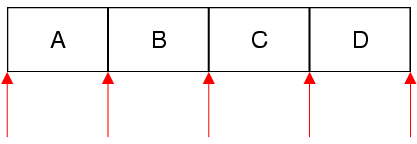
\includegraphics[width=0.5\textwidth]{qhash-iterator}
	%\caption{model index}
\end{figure}

如果想查找特定值的所有实例,循环使用 findNext()。例如:

\begin{lstlisting}[language=C++]
QHashIterator<int, QWidget *> i(hash);
while (i.findNext(widget)) {
    qDebug() << "Found widget " << widget << " under key "
             << i.key();
}
\end{lstlisting}

同一哈希表可以使用多个迭代器。如果在 QHashIterator处于活动状态时修改哈希表,QHashIterator 将继续在原哈希表上遍历,而忽略修改后的副本。


\begin{seeAlso}
QMutableHashIterator 和 QHash::const\_iterator。
\end{seeAlso}

\splitLine

\section{成员函数文档}

bool QHashIterator::findNext(const T \emph{\&value})

从当前迭代器位置开始向前查找值 \emph{value}。如果找到值为 \emph{value} 的键值对,返回 \hl{true};否则返回 \hl{false}。

调用该函数后,如果找到值 \emph{value},迭代器将被移动到匹配元素的后面;否则,
迭代器将被移动到容器的末端。

const Key \&QHashIterator::key() const

调用遍历函数((next(),findNext())后,该函数返回跳过的最后一个元素的键。

\begin{seeAlso}
value()。
\end{seeAlso}

bool QHashIterator::hasNext() const

如果该迭代器后面至少有一个元素,返回 \hl{true},即该迭代器不在容器的末端;否则返回 \hl{false}。


\begin{seeAlso}
next()。
\end{seeAlso}


void QHashIterator::toBack()

将迭代器移动到容器的末端(最后一个元素之后)。



\begin{seeAlso}
toFront()。
\end{seeAlso}


void QHashIterator::toFront()

将迭代器移动到容器的前端(第一个元素之前)。




\begin{seeAlso}
toBack() 和 next()。
\end{seeAlso}


QHashIterator<Key, T> \&QHashIterator::operator=(const QHash<Key, T> \emph{\&container})

将迭代器关联到 \emph{container} 来遍历哈希表。迭代器将被移动到哈希表的前端(第一个元素之前)。



\begin{seeAlso}
toFront() 和 toBack()。
\end{seeAlso}


QHashIterator::QHashIterator(const QHash<Key, T> \emph{\&hash})

构造一个迭代器来遍历 \emph{hash}。迭代器将被移动到哈希表的前端(第一个元素之前)。


\begin{seeAlso}
operator=()。
\end{seeAlso}


QHashIterator::Item QHashIterator::next()

返回下一个元素并将迭代器向前移动一个位置。

对返回值调用 key() 获取元素的键,调用 value() 获取元素的值。

对位于容器末端的迭代器调用该函数将导致未定义结果。



\begin{seeAlso}
hasNext() 和 peekNext()。
\end{seeAlso}

QHashIterator::Item QHashIterator::peekNext() const

不移动迭代器而返回下一个元素。

对返回值调用 key() 获取元素的键,调用 value() 获取元素的值。

对位于容器末端的迭代器调用该函数将导致未定义结果。


\begin{seeAlso}
hasNext() 和 next()。
\end{seeAlso}

const T \&QHashIterator::value() const

调用遍历函数(next(),findNext())后,该函数返回跳过的最后一个元素的值。

\begin{seeAlso}
key()。
\end{seeAlso}

%%% Local Variables:
%%% mode: latex
%%% TeX-master: "../../master"
%%% End:
\chapter{QPaintEngine}


QPaintEngine类为QPainter提供了如何在指定绘图设备上(译者注:一般为QPaintDevice的派生)绘制的一些抽象的方法。

\begin{tabular}{|l|l|}
\hline
属性 &	方法\\
\hline
头文件:& 	\#include <QPaintEngine>\\
\hline
qmake:& 	QT += core\\
\hline
\end{tabular}

\begin{notice}
此类中所有函数都是线程安全的。
\end{notice}

\section{公共成员类型}

\begin{tabular}{|l|m{23em}|}
\hline
类型 &	名称\\
\hline
enum &	LoadHint \{ ResolveAllSymbolsHint, ExportExternalSymbolsHint,
       LoadArchiveMemberHint, PreventUnloadHint, DeepBindHint \}\\
\hline
flags &	LoadHints \\ 
\hline
\end{tabular}

\section{属性}

\begin{compactitem}
\item fileName : QString
\item loadHints : LoadHints
\end{compactitem}

\section{公共成员函数}

\begin{longtable}[l]{|l|m{25em}|}
\hline
 类型& 	函数名\\
\hline
	&QLibrary(const QString \emph{\&fileName}, const QString \emph{\&version},
   QObject \emph{*parent} = nullptr)\\
\hline
	&QLibrary(const QString \emph{\&fileName}, int \emph{verNum}, QObject \emph{*parent} =
   nullptr)\\
\hline
	&QLibrary(const QString \emph{\&fileName}, QObject \emph{*parent} = nullptr)\\
\hline
	&QLibrary(QObject \emph{*parent} = nullptr)\\
\hline
virtual& 	$\sim$QLibrary()\\
\hline
QString& 	errorString() const\\
\hline
QString& 	fileName() const\\
\hline
bool& 	isLoaded() const\\
\hline
bool& 	load()\\
\hline
QLibrary::LoadHints& 	loadHints() const\\
\hline
QFunctionPointer& 	resolve(const char \emph{*symbol})\\
\hline
void& 	setFileName(const QString \emph{\&fileName})\\
\hline
void& 	setFileNameAndVersion(const QString \emph{\&fileName}, int \emph{versionNumber})\\
\hline
void& 	setFileNameAndVersion(const QString \emph{\&fileName}, const QString
      \emph{\&version})\\
\hline
void& 	setLoadHints(QLibrary::LoadHints \emph{hints})\\
\hline
bool& 	unload()\\
\hline
\end{longtable}

\section{静态公共成员}

\begin{tabular}{|l|l|}
\hline
类型& 	函数名\\
\hline
bool& 	isLibrary(const QString \&fileName)\\
\hline
QFunctionPointer& 	resolve(const QString \emph{\&fileName}, const char
                  \emph{*symbol})\\
\hline
QFunctionPointer& 	resolve(const QString \emph{\&fileName}, int \emph{verNum}, const char \emph{*symbol})\\
\hline
QFunctionPointer& 	resolve(const QString \emph{\&fileName}, const QString \emph{\&version}, const char \emph{*symbol})\\
\hline
\end{tabular}

\section{详细描述}

QLibrary的实例用于操作一个动态链接库文件(文中称为库,也就是DLL)。
QLibrary提供访问库中函数的一种平台无关方式。您可以在构造时传递库文件名,
也可以通过 setFileName() 给对象显式设置。加载库时,QLibrary在所有系统指定的位置搜索 (例如: Unix上的 LD\_LIBRARY\_PATH), 除非文件名是绝对路径。

如果文件路径是绝对路径,则会首先尝试在这个位置加载。如果找不到,
QLibrary尝试不同系统相关的前后缀的文件名,
比如Unix系的前缀“lib”,后缀“.so”,Mac及IOS的后缀".dylib",Windows的后缀".dll"。

如果文件路径不是绝对路径,Qlibrary改变搜索顺序,
首先尝试系统特定的前后缀,之后是特定文件路径。

这让使用除去前后缀的库基本名称来指定库文件变得可能。
因此代码可以在不同操作系统里执行,但不用太多代码尝试各种文件名称。

最重要的函数是 load() 用于动态加载库,isLoaded() 用于检查是否加载成功,
以及 resolve() 来解析库中的符号。如果库还没加载,resolve() 函数隐式地加载这个库。
多个QLibrary实例访问同一个物理库文件是可行的。一旦被加载,库在内存中一直保留到程序结束。
您可以通过 unload() 尝试卸载一个库,但如果有其他QLibrary实例在使用同一个库文件,调用会失败。
只有在每一个实例都调用过 unload() 后,库才会真正卸载。

Qlibrary 的一种典型用法是解析库中的导出符号,并调用其对应的C语言函数。
这叫做显式链接,对应于隐式链接。隐式链接是构建中的链接可执行文件和静态库的步骤。

下面的代码片段加载了个库,解析"mysymbol"符号,并在一切就绪的情况下调用
这个函数。如果出现了问题, 例如库文件不存在或者符号未定义,函数指针将
会是nullptr,且不会调用。

\begin{cppcode}
QLibrary myLib("mylib");
typedef void (*MyPrototype)();
MyPrototype myFunction = (MyPrototype) myLib.resolve("mysymbol");
if (myFunction)
    myFunction();
\end{cppcode}

符号必须作为C函数导出,resolve()才能工作。这意味着用C++编译器编译的函
数必须由 \hl{extern "C"}块包裹。在Windows上,还要求导出函数要使用dllexport宏;
实现详情见 resolve()。方便起见,resolve() 函数有静态形式,您可以在不现
实加载库的情况下使用:


\begin{cppcode}
typedef void (*MyPrototype)();
MyPrototype myFunction =
        (MyPrototype) QLibrary::resolve("mylib", "mysymbol");
if (myFunction)
    myFunction();
\end{cppcode}

\begin{seeAlso}
QPluginLoader.
\end{seeAlso}

\section{成员类型介绍}

enum QLibrary::LoadHint flags QLibrary::LoadHints

这个枚举描述了可能的可以用来改变库的加载行为的指示。这些取值指示在库加
载后如何解析符号,通过 setLoadHints() 指定。

\begin{tabular}{|l|l|m{20em}|}
\hline
常量 	&值& 	描述\\
\hline
QLibrary::ResolveAllSymbolsHint& 	0x01 &	在加载库的时候解析符号,而
                                           不是简单等到 resolve() 调用。
  \\
\hline
QLibrary::ExportExternalSymbolsHint& 	0x02& 	导出库中未解析的符号和
                                              外部符号,这些符号可以在
                                              后续动态加载的库中解析。
  \\
\hline
QLibrary::LoadArchiveMemberHint& 	0x04 &	运行库的文件名指定压缩包中
                                           的特定对象。如果设置了这个
                                           指示,文件名包含一个路径,
                                           其指向归档文件,接着是其中
                                           的成员名称。\\
\hline
QLibrary::PreventUnloadHint& 	0x08 	&阻止库从地址空间通过close()卸
                                        载。如果之后再有open()调用,库
                                        中的静态变量不会重新初始化。\\
\hline
QLibrary::DeepBindHint& 	0x10 	&Instructs the linker to prefer definitions in the loaded library over exported definitions in the loading application when resolving external symbols in the loaded library. This option is only supported on Linux.
命令链接器在解析加载过的库中的外部符号时,优先使用加载了的库中的定义,
  而不是在应用程序加载中的定义。【译者注:翻译存疑,故保留原文参考,详
  情参考globc--dlopen()--RTLD\_DEEPBIND】\\
\hline
\end{tabular}

LoadHints是一个 QFlags \hl{<LoadHint>} 类型的typedef。 它储存了LoadHint取值的OR(位或)方式的组合。

\begin{seeAlso}
loadHints.
\end{seeAlso}

\section{属性文档}

fileName : QString

这个属性容纳库的文件名。

我们建议忽略库的后缀名,因为Qlibrary会自动寻找带有合适后缀名的文件。 (参见 isLibrary())

当加载库时,在所有系统指定的位置搜索 (例如: Unix上的 \hl{LD\_LIBRARY\_PATH}),除非文件名是绝对路径。加载成功后,fileName() 返回返回库文件的全名。如果在构造对象或setFileName() 中包含路径,讲返回文件的全路径。

例如在Unix平台成功加载"GL"库后,fileName() 会返回 "libGL.so"。如果传递参数的文件路径是 "/usr/lib/libGL", fileName() 会返回 "/usr/lib/libGL.so"。

访问函数:

\begin{tabular}{|l|l|}
\hline
类型& 	函数名\\
\hline
QString& 	fileName() const\\
\hline
void& 	setFileName(const QString \&fileName)\\
\hline
\end{tabular}

loadHints : LoadHints

给 load() 函数一些关于如何执行的指示。

您可以对于符号如何解析做指示。通常来说,符号不是在加载库时解析的,而是惰性解析的(也就是调用 resolve() 时)。
如果您设置loadHints 为ResolveAllSymbolsHint,那么如果平台支持,所有符号会在库加载时一齐解析。

设置 ExportExternalSymbolsHint 会使库中的外部符号在后续库解析中可用。

如果设置了 LoadArchiveMemberHint ,文件名会被分解为两部分:归档文件的路径和归档成员的名称。
例如, fileName libGL.a(\hl{shr\_64.o}) 指向归档文件 \hl{libGL.a}中的库文件 \hl{shr\_64.o} 。
这个特性只在AIX平台生效。

loadHints 的解释是平台相关的,如果您用这些特效,您大概已经对编译的系统平台做了一些假设。
因此请仅在您明白您这些操作的结果的情况下设置这些指示。

默认情况下,此属性没有设置任何flag,所有库文件会惰性加载,
并且不会导出共其他动态链接库使用的外部符号。

\begin{notice}
在库已经加载后设置这个属性没有效果。 并且 loadHints() 不会体现出这些修
改。
\end{notice}

\begin{notice}
这个属性是所有指向同一个库的 QLibrary 实例共享的。
\end{notice}

访问函数:

\begin{tabular}{|l|l|}
\hline
类型 	&函数名\\
\hline
QLibrary::LoadHints &	loadHints() const\\
\hline
void &	setLoadHints(QLibrary::LoadHints \emph{hints})\\
\hline
\end{tabular}

\section{成员函数文档}

% gog 

QLibrary::QLibrary(const QString \emph{\&fileName}, const QString \emph{\&version}, QObject \emph{*parent} = nullptr)

基于给定的父对象 \emph{parent} 构造一个库对象。它会加载文件名 \emph{fileName}、完整版本号 \emph{version} 指定的库文件。如今,版本号在Windows上被忽略。

我们建议在 \emph{fileName} 中忽略文件名的前后缀,因为QLibrary会基于不同平台自
动寻找合适的前后缀。比如Unix系的前缀“lib”,后缀“.so”,Mac及IOS的后缀
".dylib",Windows的后缀".dll"。(参见fileName )

QLibrary::QLibrary(const QString \emph{\&fileName}, int \emph{verNum}, QObject \emph{*parent} = nullptr)

基于给定的父对象 \emph{parent} 构造一个库对象。它会加载文件名 \emph{fileName}、主版本号 \emph{verNum} 指定的库文件。如今,版本号在Windows上被忽略。

我们建议在 fileName 中忽略文件名的前后缀,因为QLibrary会基于不同平台自
动寻找合适的前后缀。比如Unix系的前缀“lib”,后缀“.so”,Mac及IOS的后缀
".dylib",Windows的后缀".dll"。(参见fileName )

QLibrary::QLibrary(const QString \emph{\&fileName}, QObject
\emph{*parent} = nullptr)

基于给定的父对象 \emph{parent} 构造一个库对象。它会加载文件名 \emph{fileName} 指定的库文件。

我们建议在 
\emph{fileName} 中忽略文件名的前后缀,因为QLibrary会基于不同平台自
动寻找合适的前后缀。比如Unix系的前缀“lib”,后缀“.so”,Mac及IOS的后缀
".dylib",Windows的后缀".dll"。(参见fileName )

QLibrary::QLibrary(QObject \emph{*parent} = nullptr)

基于给定的父对象 \emph{parent} 构造一个库对象。

\hl{[virtual]}QLibrary::$\sim$QLibrary()

删除此QLibrary对象。

除非显式调用 unload(),库会在一直驻留在内存中,知道应用结束。

\begin{seeAlso}
isLoaded() 和 unload().
\end{seeAlso}


QString QLibrary::errorString() const

返回一个描述上一个发生的错误的文本字符串。截至现在,errorString 只会在 load(), unload() 或 resolve() 调用由于一些原因失败时才会设置。

此函数引入自:Qt 4.2.


\hl{[static]}bool QLibrary::isLibrary(const QString \emph{\&fileName})

如果 \emph{fileName} 包含一个合法的可加载的后缀,返回true;否则返回false。

\begin{tabular}{|c|c|}
\hline
平台& 	合法后缀\\
\hline
Windows& 	.dll, .DLL\\
\hline
Unix/Linux& 	.so\\
\hline
AIX 	&.a\\
\hline
HP-UX 	&.sl, .so (HP-UXi)\\
\hline
macOS and iOS& 	.dylib, .bundle, .so\\
\hline
\end{tabular}

Unix平台上的名字后的版本号会被忽略。

bool QLibrary::isLoaded() const

如果库已经被加载,返回true,否则返回false。

\begin{seeAlso}
load().
\end{seeAlso}

bool QLibrary::load()

加载一个库,如果成功加载则返回true;否则返回false。因为 resolve() 内部会自动调用此方法,您没必要显示调用这个函数。如果在某些情况下您想提前加载库,您可以主动调用它。

\begin{seeAlso}
unload().
\end{seeAlso}

QFunctionPointer QLibrary::res
olve(const char \emph{*symbol})

返回导出符号 \emph{symbol} 对应的地址。如果需要,库会自动加载。如果库无法加载或符号无法解析,返回 \hl{nullptr} 。

例如:

\begin{cppcode}
typedef int (*AvgFunction)(int, int);

AvgFunction avg = (AvgFunction) library->resolve("avg");
if (avg)
    return avg(5, 8);
else
    return -1;
\end{cppcode}

符号必须作为C语言函数导出。这意味着如果使用C++编译器,函数必须由
\hl{extern "C"} 包裹。在Windows平台,您还必须显式通过 \hl{\_\_declspec(dllexport)}
指导编译器导出符号,例如:

\begin{cppcode}
extern "C" MY_EXPORT int avg(int a, int b)
{
    return (a + b) / 2;
}
\end{cppcode}

宏 \hl{MY\_EXPORT} 定义如下

\begin{cppcode}
#ifdef Q_OS_WIN
#define MY_EXPORT __declspec(dllexport)
#else
#define MY_EXPORT
#endif
\end{cppcode}


% gog 


\hl{[static]}QFunctionPointer QLibrary::resolve(const QString \emph{\&fileName}, const char \emph{*symbol})

这是一个重载函数。

加载文件名 \emph{fileName} 对应的库,并返回 \emph{symbol} 对应导出符号的地址。注意 \emph{fileName} 不应该包含平台相关前后缀(详情见 fileName). 库会一直保留到应用程序退出。

如果库无法加载或符号无法解析,返回 \hl{nullptr} 。

\begin{seeAlso}
resolve().
\end{seeAlso}

\hl{[static]}QFunctionPointer QLibrary::resolve(const QString
\emph{\&fileName}, int \emph{verNum}, const char \emph{*symbol})

这是一个重载函数。

加载文件名 \emph{fileName} 、主版本号 \emph{verNum} 对应的库,并返回 \emph{symbol} 对应导出符号的地址。注意 \emph{fileName} 不应该包含平台相关前后缀(详情见 fileName). 库会一直保留到应用程序退出。\emph{version} 参数在 Windows 上无效。

如果库无法加载或符号无法解析,返回 \hl{nullptr} 。

\begin{seeAlso}
resolve().
\end{seeAlso}

[static]QFunctionPointer QLibrary::resolve(const QString \emph{\&fileName}, const QString \emph{\&version}, const char \emph{*symbol})

这是一个重载函数。

加载文件名 \emph{fileName}、完整版本号 \emph{version} 对应的库,并返回 \emph{symbol} 对应导出符号的地址。注意 \emph{fileName} 不应该包含平台相关前后缀(详情见 fileName). 库会一直保留到应用程序退出。\emph{version} 参数在 Windows 上无效。

如果库无法加载或符号无法解析,返回 \hl{nullptr} 。

此函数引入自:Qt 4.4.

\begin{seeAlso}
resolve().
\end{seeAlso}

void QLibrary::setFileNameAndVersion(const QString \emph{\&fileName}, int \emph{versionNumber})

设置 \emph{fileName} 属性,以及相对应的文件名和版本号信息。\emph{versionNumber} 参数在 Windows 上无效。



\begin{seeAlso}
setFileName().
\end{seeAlso}


void QLibrary::setFileNameAndVersion(const QString \emph{\&fileName}, const
QString \emph{\&version})

设置 \emph{fileName} 属性,以及相对应的文件名和完整版本号信息。\emph{version} 参数在 Windows 上无效。

此函数引入自:Qt 4.4.

\begin{seeAlso}
setFileName().
\end{seeAlso}

bool QLibrary::unload()

卸载一个库;如果成功返回 \hl{true},否则 \hl{false}。

在应用程序结束是,此函数自动调用,因此您不应该手动调用。

如果有其他 QLibrary 示例在使用同一个库,调用会失败。卸载只会在所有实例都调用过此函数之后发生。

\begin{notice}
在 Mac OS X 10.3 (Panther),无法卸载动态链接库。
\end{notice}

\begin{seeAlso}
resolve() 和 load().
\end{seeAlso}
\chapter{QPluginLoader}

QPluginLoader 在运行时加载插件。

\begin{tabular}{|l|l|}
\hline
属性 &	方法\\
\hline
头文件:& 	\#include <QPluginLoader>\\
\hline
qmake:& 	QT += core\\
\hline
继承:	&  \href{https://gitee.com/wcc210/QtDocumentCN/blob/master/Src/O/QObject/QObject.md}{QObject} \\
\hline
\end{tabular}

\begin{notice}
该类提供的所有函数都是可重入的。
\end{notice}


\section{属性}


\begin{tabular}{|l|l|}
\hline
属性 &	类型\\
\hline
fileName &	QString \\ 
\hline
loadHints	& QLibrary::LoadHints \\ 
\hline
\end{tabular}

\section{公共成员函数}

\begin{longtable}[l]{|l|m{25em}|}
\hline
 类型& 	函数名\\
\hline
& QPluginLoader(const QString \emph{\&*fileName}, QObject \emph{*parent} = nullptr) \\
\hline
&QPluginLoader(QObject *parent = nullptr) \\
\hline
virtual	&$\sim$QPluginLoader() \\
\hline
QString	&errorString() const \\
\hline
QString	&fileName() const \\
\hline
QObject *	&instance() \\
\hline
bool	&isLoaded() const \\
\hline
bool	&load() \\
\hline
QLibrary::LoadHints	&loadHints() const \\
\hline
QJsonObject	&metaData() const \\
\hline
void	&setFileName(const QString \emph{\&fileName}) \\
\hline
void&	setLoadHints(QLibrary::LoadHints \emph{loadHints}) \\
\hline
bool&	unload() \\
\hline
\end{longtable}

\section{静态公共成员函数}

\begin{tabular}{|l|l|}
\hline
返回类型& 	函数名\\
\hline
QObjectList	&staticInstances() \\
\hline
QVector<QStaticPlugin> &	staticPlugins() \\
\hline
\end{tabular}


\section{相关的非成员函数}

\begin{tabular}{|l|l|}
\hline
返回类型& 	函数名\\
\hline
void	& qRegisterStaticPluginFunction(QStaticPlugin \emph{plugin}) \\
\hline
\end{tabular}


\section{详细介绍}

QPluginLoader 提供对 Qt 插件的访问。
Qt 插件存储在共享库(DLL)中,而相比使用 QLibrary 访问的共享库,它具有以下优点:

\begin{compactitem}
\item QPluginLoader 检查插件是否链接到与应用程序相同的 Qt 版本。
\item QPluginLoader 提供对根组件对象的直接访问(instance()),而无需手动解析C函数。
\end{compactitem}

QPluginLoader对象的实例在被称为插件的单个共享库文件上运行。
它以独立于平台的方式提供对插件中功能的访问。
要指定加载的插件,可以在构造函数中传递文件名,或者通过 setFileName() 进行设置。

最重要的函数有:用来动态加载插件文件的 load(),
用来检查加载是否成功的 isLoaded() , 以及用来访问插件根组件的 instance()。
如果尚未加载插件,则 instance() 函数会隐式尝试加载该插件。
 可以使用 QPluginLoader 的多个实例来访问同一个实际的插件。

加载后,插件将保留在内存中,直到所有 QPluginLoader 实例都已卸载,或者应用程序终止为止。
您可以使用 unload() 来尝试卸载插件,但如果有其它 QPluginLoader 实例正在使用同一个库,
那么这一函数调用会失败,而当所有实例都调用了 unload() 后插件才会真正被卸载。
在卸载发生之前,根组件也将被删除。

有关如何使应用程序可通过插件扩展的更多信息,请参见如何创建 Qt 插件。

请注意,如果您的应用程序与 Qt 静态链接,则无法使用 QPluginLoader。
在这种情况下,您还必须静态链接到插件。
如果需要在静态链接的应用程序中加载动态库,则可以使用 QLibrary。

\begin{seeAlso}
QLibrary 和插件与绘制示例。
\end{seeAlso}

\section{属性文档}

fileName : QString

该属性记录插件的文件名。

我们建议在文件名中省略文件的后缀,因为 QPluginLoader 将自动查找具有适当后缀的文件(请参阅 QLibrary::isLibrary())。

加载插件时,除非文件名具有绝对路径,
否则 QPluginLoader 会搜索 QCoreApplication::libraryPaths() 指定的所有插件位置。
成功加载插件后,fileName() 返回插件的完全限定文件名,
如果在构造函数中已指定或传递给 setFileName(),则包括插件的完整路径。

如果文件名不存在,改属性将不会设置,并包含一个空字符串。

默认情况下,该属性包含一个空字符串。

存取函数


\begin{tabular}{|l|l|}
\hline
返回类型& 	函数名\\
\hline
QString	& fileName() const \\ 
\hline
void	& setFileName(const QString \emph{\&fileName}) \\ 
\hline
\end{tabular}

\begin{seeAlso}
load()。
\end{seeAlso}

loadHints : QLibrary::LoadHints

为 load() 函数提供一些有关其行为方式的提示。

您可以提供有关如何解析插件中符号的提示。
从 Qt 5.7 起,默认设置为 QLibrary::PreventUnloadHint。

有关该属性如何工作的完整说明,请参阅 QLibrary::loadHints 的文档。

该属性在 Qt 4.4 中引入。

存取函数

\begin{tabular}{|l|l|}
\hline
返回类型& 	函数名\\
\hline
QLibrary::LoadHints	& loadHints() const \\ 
\hline
void & setLoadHints(QLibrary::LoadHints \emph{loadHints}) \\
\hline
\end{tabular}

\begin{seeAlso}
QLibrary::loadHints。
\end{seeAlso}

\section{成员函数文档}

%%%%%%%%%%%%%%%%%%%%%%%%%%%%

QPluginLoader::QPluginLoader(const QString \&fileName, QObject *parent = nullptr)

使用给定的 parent 构造一个插件加载器,并加载 fileName 指定的插件。

为了可加载,文件的后缀必须是可加载库的有效后缀,具体取决于平台,例如,Unix 上的 .so,macOS 和 iOS .dylib,以及 Windows 上的 .dll。后缀可以通过 QLibrary::isLibrary() 验证。

\begin{seeAlso}
setFileName()。
\end{seeAlso}

QPluginLoader::QPluginLoader(QObject \emph{*parent} = nullptr)

使用给定的 parent 构造一个插件加载器。

[virtual]QPluginLoader::$\sim$QPluginLoader()

销毁 QPluginLoader 对象。

除非 unload() 被显式调用,插件会一直留在内存中直到程序结束。

\begin{seeAlso}
isLoaded() 和 unload()。
\end{seeAlso}

QString QPluginLoader::errorString() const

返回带有最后发生的错误描述文本的字符串。

该函数在 Qt 4.2 中引入。

QObject *QPluginLoader::instance()

返回插件的根组件对象。必要时会加载插件。
如果无法加载插件或者根组件对象无法实例化时,该函数将返回 \hl{nullptr}。

如果根组件对象已经被销毁了,该函数在调用时会创建一个新的实例。

该函数返回的根组件不会随着 QPluginLoader 的销毁而被删除。
如果您希望保证根组件会被删除,可以在您不再需要访问核心组件是立即调用 unload()。
当库最终卸载时,对应根组件也会自动删除。

组件对象是一个 QObject。使用 qobject\_cast() 来访问你想要的接口。

\begin{seeAlso}
load()。
\end{seeAlso}

bool QPluginLoader::isLoaded() const

如果已经成功加载插件则返回 \hl{true},否则返回 \hl{false}。

\begin{seeAlso}
load()。
\end{seeAlso}

bool QPluginLoader::load()

加载插件,并在插件成功加载时返回 \hl{true},否则返回 \hl{false}。
由于 instance() 始终在解析任何符号之前调用此函数,因此无需显式调用它。
在某些情况下,您可能需要预先加载插件,这时您才要使用该函数。

\begin{seeAlso}
unload()。
\end{seeAlso}

QJsonObject QPluginLoader::metaData() const

返回该插件的元数据。元数据是在编译插件时使用 Q\_PLUGIN\_METADATA() 宏以json格式指定的数据。

无需实际加载插件即可以快速又经济的方式查询元数据。
这使得例如可以在其中储存插件的功能,并根据该元数据来决定是否加载插件。

[static]QObjectList QPluginLoader::staticInstances()

返回由插件加载器保存的静态插件实例(根组件)的列表。

另请参阅 staticPlugins()。

[static]QVector<QStaticPlugin> QPluginLoader::staticPlugins()

返回由插件加载器保存的 QStaticPlugins 列表。 
该函数类似于 staticInstances(),
除了 QStaticPlugin 还包含元数据信息。

\begin{seeAlso}
staticInstances()。
\end{seeAlso}

bool QPluginLoader::unload()

卸载插件,并在插件卸载成功时返回 \hl{true},否则返回 \hl{false}。
这会在应用程序终止时自动发生,因此您通常不需要调用此函数。
如果存在其它 QPluginLoader 实例正在使用同一个插件,调用会失败,
卸载只会发生在所有实例都调用了 \hl{unload()} 时。
不要试图删除根组件。
相反,凭借 \hl{unload()} ,它会在必要时自动将其删除。

\begin{seeAlso}
instance() 和 load()。
\end{seeAlso}

\section{相关的非成员函数}

void qRegisterStaticPluginFunction(QStaticPlugin \emph{plugin})

注册由插件加载器指定的 \emph{plugin},并由 Q\_IMPORT\_PLUGIN() 使用。

该函数在 Qt 5.0 中引入。

\chapter{QtPlugin}

QtPlugin 头文件定义用于定义插件的宏。

\begin{tabular}{|l|l|}
\hline
属性 &	方法\\
\hline
头文件:& 	\#include <QtPlugin>\\
\hline
\end{tabular}

\section{宏}

\begin{tabular}{|l|}
\hline
宏名 \\
\hline
Q\_DECLARE\_INTERFACE(ClassName, Identifier) \\ 
\hline
Q\_IMPORT\_PLUGIN(PluginName) \\ 
\hline
Q\_PLUGIN\_METADATA(...) \\
\hline
\end{tabular}




%%%%%%%%%%%

\section{详细介绍}
另请参阅 如何创建 Qt 插件。

\section{宏文档}

Q\_DECLARE\_INTERFACE(ClassName, Identifier)

该宏将给定的 Identifier(字符串字面量)与名为 ClassName 的接口类关联。
Identifier 必须是唯一的。例如:

\begin{lstlisting}[language=C++]
#define BrushInterface_iid "org.qt-project.Qt.Examples.PlugAndPaint.BrushInterface/1.0"

Q_DECLARE_INTERFACE(BrushInterface, BrushInterface_iid)
\end{lstlisting}

通常在头文件中 ClassName 的类定义之后立即使用此宏。有关详细信息,请参见插件与绘制示例。

如果要对命名空间中的接口类使用 Q\_DECLARE\_INTERFACE,请务必保证 Q\_DECLARE\_INTERFACE 不在命名空间中。例如:

\begin{lstlisting}[language=C++]
namespace Foo
{
    struct MyInterface { ... };
}

Q_DECLARE_INTERFACE(Foo::MyInterface, "org.examples.MyInterface")
\end{lstlisting}

\begin{lstlisting}[language=C++]
Q\_INTERFACES() 和如何创建 Qt 插件。
\end{lstlisting}

Q\_IMPORT\_PLUGIN(PluginName)

该宏导入名为 PluginName 的插件,
该插件与使用 Q\_PLUGIN\_METADATA() 声明插件元数据的类的名称相对应。

将该宏插入应用程序的源代码来使您能够使用静态插件。

例如:

\begin{lstlisting}[language=C++]
Q_IMPORT_PLUGIN(qjpeg)
\end{lstlisting}

构建应用程序时,链接器必须包含静态插件。对于 Qt 预定义的插件,可以使用 QTPLUGIN 将插件加入你的构建系统。例如:

\begin{lstlisting}[language=C++]
TEMPLATE      = app
QTPLUGIN     += qjpeg qgif    # image formats
\end{lstlisting}


\begin{seeAlso}
 静态插件、如何创建 Qt 插件以及 qmake 入门。
\end{seeAlso}

Q\_PLUGIN\_METADATA(...)

该宏用于声明插件元数据,它是实例化此对象的插件的一部分。

该宏需要声明通过该对象实现的接口的 IID,并引用包含该插件的元数据的文件。

对于某一个 Qt 插件,该宏在源代码中应恰好出现一次。

示例:

\begin{lstlisting}[language=C++]
class MyInstance : public QObject
{
    Q_PLUGIN_METADATA(IID "org.qt-project.Qt.QDummyPlugin" FILE "mymetadata.json")
};
\end{lstlisting}

有关详细信息,请参见插件与绘制示例。

请注意,该宏出现的类必须是可默认构造的。

FILE是可选的,并指向一个 json 文件。

该 json 文件必须存在于构建系统指定的包含目录之一中。当找不到指定文件时,moc 将退出并显示错误。

该宏在 Qt 5.0 中引入。

\begin{seeAlso}
Q\_DECLARE\_INTERFACE() 和如何创建 Qt 插件。
\end{seeAlso}
\chapter{Qt概述}

Qt 提供了覆盖广泛领域的各类技术。以下话题关键功能领域,并且可以用作学习如何充分利用 Qt 的起点。

\begin{compactitem}[\arr]
\item 开发工具
\item 用户界面
\item 核心内部构件
\item 数据存储
\item 多媒体
\item 网络和连接
\item 图形
\item 集成 Web 内容
\item 移动 API
\item QML 应用程序
\item 脚本
\item Qt 国际化
\item 测试和调试
\item 从 Qt 4 移植
\end{compactitem}


\section{最佳实践}

详见\href{https://gitee.com/wcc210/QtDocumentCN/blob/master/Src/B/Best_Practice_Guides/Best_Practice_Guides.md}{最佳实践指南。}


\section{参考}

\begin{seeAlso}
所有概述页面来查看所有概述文章、C++ 模块、QML 模块的列表
\end{seeAlso}


\chapter{QJsonParseError}

QJsonParseError类用于在JSON解析期间报告错误。

\begin{tabular}{|r|l|}
	\hline
	属性 & 方法 \\
	\hline
	头文件 & \#include<QJsonParseError>\\      
	\hline
	qmake & QT+=core\\      
	\hline
	自从 & Qt5.0\\
	\hline
	继承&QObject \\
	\hline
\end{tabular}

该结构在 5.0 被引入。

\textbf{注意}: 该结构的所有函数都是可重入。


\section{公共类型}

\begin{tabular}{|l|l|}
	\hline
	类型& 	枚举\\
\hline
enum &	ParseError { NoError, UnterminatedObject, MissingNameSeparator, UnterminatedArray, MissingValueSeparator, …, GarbageAtEnd }\\
	\hline
\end{tabular}


\section{公共成员函数}


\begin{tabular}{|l|l|}
	\hline
类型 &	函数名\\
\hline
QString &	errorString() const\\
	\hline
\end{tabular}


\section{公共变量}

\begin{tabular}{|l|l|}
\hline
类型 	&变量名\\
\hline
QJsonParseError::ParseError& 	error\\
\hline
int 	&offset\\
\hline
\end{tabular}


\section{详细说明}

\textbf{另外参阅}: JSON Support in Qt 和 JSON Save Game Example。


\section{成员类型文档}

enum QJsonParseError::ParseError

该枚举描述了在解析JSON文档期间发生的错误类型。

\begin{longtable}{|l|l|l|}
\hline
不变量& 	值& 	描述\\
\hline
QJsonParseError::NoError& 	0& 	没有发生错误\\
\hline
QJsonParseError::UnterminatedObject& 	1& 	对象未正确使用大括号\\
\hline
QJsonParseError::MissingNameSeparator& 	2& 	缺少分隔不同项目的逗号\\
\hline
QJsonParseError::UnterminatedArray& 	3& 	数组未正确用方括号括起来\\
\hline
QJsonParseError::MissingValueSeparator& 	4& 	缺少将键与对象内的值分
                                               隔开的冒号\\
\hline
QJsonParseError::IllegalValue& 	5& 	该值是非法的\\
\hline
QJsonParseError::TerminationByNumber& 	6& 	输入流在解析数字时结束\\
\hline
QJsonParseError::IllegalNumber& 	7& 	数字格式不正确\\
\hline
QJsonParseError::IllegalEscapeSequence& 	8& 	输入中发生非法的转义序
                                               列\\
\hline
QJsonParseError::IllegalUTF8String& 	9& 	输入中出现非法的UTF8序列\\
\hline
QJsonParseError::UnterminatedString& 	10& 	字符串未以引号终止\\
\hline
QJsonParseError::MissingObject& 	11& 	预期有对象,但找不到\\
\hline
QJsonParseError::DeepNesting& 	12& 	JSON文档的嵌套太深,解析器无法对其进行解析\\
\hline
QJsonParseError::DocumentTooLarge& 	13& 	JSON文档太大,解析器无法解析它\\
\hline
QJsonParseError::GarbageAtEnd& 	14& 	解析的文档末尾包含其他垃圾字符\\
\hline
\end{longtable}


\section{公有成员函数文档}

QString QJsonParseError::errorString() const

返回适合于所报告的JSON解析错误的人类可读消息。

\textbf{另请参见}: error。


\section{成员变量文档}

QJsonParseError::ParseError QJsonParseError::error

包含解析错误的类型。如果文档被正确解析,则等于QJsonParseError::NoError。

\textbf{另外参阅}: ParseError 和 errorString()。

int QJsonParseError::offset

包含发生解析错误的输入字符串中的偏移量。

\textbf{另外参阅}: error 和 errorString()。

%%% Local Variables:
%%% mode: latex
%%% TeX-master: "../../master"
%%% End:

\chapter{QKeyValueIterator}


template <typename Key, typename T, typename Iterator> class QKeyValueIterator

关联容器的键值对类型的迭代器。更多内容...

\begin{tabular}{|r|l|}
	\hline
	属性 & 方法 \\
	\hline
	头文件 & \#include<QKeyValueIterator>\\      
	\hline
	qmake & QT+=core\\      
	\hline
	Since:&	Qt 5.10 \\ 
	\hline
\end{tabular}

Qt 5.10 中引入该类。

\begin{compactitem}
\item 所有成员列表,包括继承的成员
\end{compactitem}

\section{公共成员函数}

\begin{tabular}{|l|l|}
\hline
类型 &	函数名\\
\hline
& QKeyValueIterator(Iterator \emph{o}) \\ 
\hline
& QKeyValueIterator() \\ 
\hline
Iterator	& base() const \\ 
\hline
std::pair<Key, T>	& operator*() const \\ 
\hline
QKeyValueIterator<Key, T, Iterator> \&	& operator++() \\ 
\hline
QKeyValueIterator<Key, T, Iterator>	& operator++(\emph{int}) \\ 
\hline
QKeyValueIterator<Key, T, Iterator> \& &	operator--() \\ 
\hline
QKeyValueIterator<Key, T, Iterator>	 &operator--(\emph{int}) \\ 
\hline
QKeyValueIterator::pointer &	operator->() const \\ 
\hline
\end{tabular}

\section{相关非成员函数}

\begin{tabular}{|l|m{30em}|}
\hline
类型 	&函数名\\
\hline
bool & operator!=(QKeyValueIterator<Key, T, Iterator> \emph{lhs
}, QKeyValueIterator<Key, T, Iterator> \emph{rhs}) \\ 
\hline
bool &	operator==(QKeyValueIterator<Key, T, Iterator> \emph{lhs}, QKeyValueIterator<Key, T, Iterator> \emph{rhs}) \\ 
\hline
\end{tabular}

\section{详细描述}

QKeyValueIterator 类为关联容器如 QHash 和 QMap 返回的键值对提供 STL 风格的迭代器。
该类支持与 STL 关联容器相同的接口,即遍历容器时取得键值对。

这将改善 QMap,QHash 及其相关类与 STL 风格算法之间的互操作性。

\begin{warning}
隐式共享容器的迭代器的工作方式和 STL 迭代器不完全相同。当容器的迭代器还处于活动状态时,应该避免拷贝容器。更多信息请参阅隐式共享迭代器问题
\end{warning}

\section{成员函数文档}

QKeyValueIterator::QKeyValueIterator(Iterator \emph{o})

在迭代器 \emph{o} 之上构造 QKeyValueIterator。

QKeyValueIterator::QKeyValueIterator()

构造一个默认 QKeyValueIterator。

Iterator QKeyValueIterator::base() const

返回该 QKeyValueIterator 基于的底层迭代器。

std::pair<Key, T> QKeyValueIterator::operator*() const

以键值对返回当前元素。

QKeyValueIterator<Key, T, Iterator> \&QKeyValueIterator::operator++()

前置 ++ 运算符(\hl{++i})将迭代器向前移动到容器中的下一个元素并返回迭代器。

\begin{notice}
将迭代器向前移动到容器的 end() 之后将导致未定义行为。
\end{notice}

\begin{seeAlso}
operator--()。
\end{seeAlso}

QKeyValueIterator<Key, T, Iterator> QKeyValueIterator::operator++(int)

这是一个重载函数。

后置 ++ 运算符(\hl{i++})将迭代器向前移动到容器中的下一个元素并返回指向旧位置元素的迭代器。

\begin{notice}
将迭代器向前移动到容器的 end() 之后将导致未定义行为。
\end{notice}

QKeyValueIterator<Key, T, Iterator> \&QKeyValueIterator::operator--()

前置 -- 运算符(\hl{--i})将迭代器向后前移动到容器中的前一个元素并返回迭代器。

\begin{notice}
将迭代器向后移动到容器的 begin() 之前将导致未定义行为。
\end{notice}

\begin{seeAlso}
operator++()。
\end{seeAlso}

QKeyValueIterator<Key, T, Iterator> QKeyValueIterator::operator--(\emph{int})

这是一个重载函数。

后置 -- 运算符(\hl{i--})将迭代器向后前移动到容器中的前一个元素并返回指向旧位置元素的迭代器。

\begin{notice}
将迭代器向后移动到容器的 begin() 之前将导致未定义行为。
\end{notice}

QKeyValueIterator::pointer QKeyValueIterator::operator->() const

返回指向当前元素的键值对类型的指针。

Qt 5.15 中引入该函数。

\begin{seeAlso}
operator*()。
\end{seeAlso}

\section{相关非成员函数}

bool operator!=(QKeyValueIterator<Key, T, Iterator> \emph{lhs}, QKeyValueIterator<Key, T, Iterator> \emph{rhs})

如果 \emph{rhs} 与 \emph{lhs} 指向的元素不同,返回 \hl{true},否则返回 \hl{false}。

\begin{seeAlso}
operator==()。
\end{seeAlso}

bool operator==(QKeyValueIterator<Key, T, Iterator> \emph{lhs}, QKeyValueIterator<Key, T, Iterator> \emph{rhs})

如果 \emph{rhs} 与 \emph{lhs} 指向的元素相同,返回 \hl{true},否则返回 \hl{false}。

\begin{seeAlso}
operator!=()。
\end{seeAlso}
\chapter{QLibrary}

Qlibrary用于运行时加载库。

\begin{tabular}{|l|l|}
\hline
属性 &	内容\\
\hline
头文件:& 	\#include <QLibrary>\\
\hline
qmake:& 	QT += core\\
\hline
继承于:& 	QObject\\
\hline
\end{tabular}

\begin{notice}
此类中全部函数可重入。
\end{notice}

\section{公共成员类型}

\begin{tabular}{|l|m{23em}|}
\hline
类型 &	名称\\
\hline
enum &	LoadHint { ResolveAllSymbolsHint, ExportExternalSymbolsHint,
       LoadArchiveMemberHint, PreventUnloadHint, DeepBindHint }\\
\hline
flags &	LoadHints \\ 
\hline
\end{tabular}

\section{属性}

\begin{compactitem}[\arr]
\item fileName : QString
\item loadHints : LoadHints
\end{compactitem}

\section{公共成员函数}

\begin{longtable}[l]{|l|m{25em}|}
\hline
 类型& 	函数名\\
\hline
	&QLibrary(const QString \&fileName, const QString \&version,
   QObject *parent = nullptr)\\
\hline
	&QLibrary(const QString \&fileName, int verNum, QObject *parent =
   nullptr)\\
\hline
	&QLibrary(const QString \&fileName, QObject *parent = nullptr)\\
\hline
	&QLibrary(QObject *parent = nullptr)\\
\hline
virtual& 	$\sim$QLibrary()\\
\hline
QString& 	errorString() const\\
\hline
QString& 	fileName() const\\
\hline
bool& 	isLoaded() const\\
\hline
bool& 	load()\\
\hline
QLibrary::LoadHints& 	loadHints() const\\
\hline
QFunctionPointer& 	resolve(const char *symbol)\\
\hline
void& 	setFileName(const QString \&fileName)\\
\hline
void& 	setFileNameAndVersion(const QString \&fileName, int versionNumber)\\
\hline
void& 	setFileNameAndVersion(const QString \&fileName, const QString
      \&version)\\
\hline
void& 	setLoadHints(QLibrary::LoadHints hints)\\
\hline
bool& 	unload()\\
\hline
\end{longtable}

\section{静态公共成员}

\begin{tabular}{|l|l|}
\hline
类型& 	函数名\\
\hline
bool& 	isLibrary(const QString \&fileName)\\
\hline
QFunctionPointer& 	resolve(const QString \&fileName, const char
                  *symbol)\\
\hline
QFunctionPointer& 	resolve(const QString \&fileName, int verNum, const char *symbol)\\
\hline
QFunctionPointer& 	resolve(const QString \&fileName, const QString \&version, const char *symbol)\\
\hline
\end{tabular}

\section{详细描述}

QLibrary的实例用于操作一个动态链接库文件(文中称为库,也就是DLL)。QLibrary提供访问库中函数的一种平台无关方式。您可以在构造时传递库文件名,也可以通过 setFileName() 给对象显式设置。加载库时,QLibrary在所有系统指定的位置搜索 (例如: Unix上的 LD\_LIBRARY\_PATH), 除非文件名是绝对路径。

如果文件路径是绝对路径,则会首先尝试在这个位置加载。如果找不到,QLibrary尝试不同系统相关的前后缀的文件名,比如Unix系的前缀“lib”,后缀“.so”,Mac及IOS的后缀".dylib",Windows的后缀".dll"。

如果文件路径不是绝对路径,Qlibrary改变搜索顺序,首先尝试系统特定的前后缀,之后是特定文件路径。

这让使用除去前后缀的库基本名称来指定库文件变得可能。因此代码可以在不同操作系统里执行,但不用太多代码尝试各种文件名称。

最重要的函数是 load() 用于动态加载库,isLoaded() 用于检查是否加载成功,以及 resolve() 来解析库中的符号。如果库还没加载,resolve() 函数隐式地加载这个库。多个QLibrary实例访问同一个物理库文件是可行的。一旦被加载,库在内存中一直保留到程序结束。您可以通过 unload() 尝试卸载一个库,但如果有其他QLibrary实例在使用同一个库文件,调用会失败。只有在每一个实例都调用过 unload() 后,库才会真正卸载。

Qlibrary 的一种典型用法是解析库中的导出符号,并调用其对应的C语言函数。这叫做显式链接,对应于隐式链接。隐式链接是构建中的链接可执行文件和静态库的步骤。

下面的代码片段加载了个库,解析"mysymbol"符号,并在一切就绪的情况下调用
这个函数。如果出现了问题, 例如库文件不存在或者符号未定义,函数指针将
会是nullptr,且不会调用。

\begin{lstlisting}[language=C++]
QLibrary myLib("mylib");
typedef void (*MyPrototype)();
MyPrototype myFunction = (MyPrototype) myLib.resolve("mysymbol");
if (myFunction)
    myFunction();
\end{lstlisting}

符号必须作为C函数导出,resolve()才能工作。这意味着用C++编译器编译的函
数必须由 \hl{extern "C"}块包裹。在Windows上,还要求导出函数要使用dllexport宏;
实现详情见 resolve()。方便起见,resolve() 函数有静态形式,您可以在不现
实加载库的情况下使用:


\begin{lstlisting}[language=C++]
typedef void (*MyPrototype)();
MyPrototype myFunction =
        (MyPrototype) QLibrary::resolve("mylib", "mysymbol");
if (myFunction)
    myFunction();
\end{lstlisting}

\begin{seeAlso}
QPluginLoader.
\end{seeAlso}

\section{成员类型介绍}

enum QLibrary::LoadHint flags QLibrary::LoadHints

这个枚举描述了可能的可以用来改变库的加载行为的指示。这些取值指示在库加
载后如何解析符号,通过 setLoadHints() 指定。

\begin{tabular}{|l|l|m{20em}|}
\hline
常量 	&值& 	描述\\
\hline
QLibrary::ResolveAllSymbolsHint& 	0x01 &	在加载库的时候解析符号,而
                                           不是简单等到 resolve() 调用。
  \\
\hline
QLibrary::ExportExternalSymbolsHint& 	0x02& 	导出库中未解析的符号和
                                              外部符号,这些符号可以在
                                              后续动态加载的库中解析。
  \\
\hline
QLibrary::LoadArchiveMemberHint& 	0x04 &	运行库的文件名指定压缩包中
                                           的特定对象。如果设置了这个
                                           指示,文件名包含一个路径,
                                           其指向归档文件,接着是其中
                                           的成员名称。\\
\hline
QLibrary::PreventUnloadHint& 	0x08 	&阻止库从地址空间通过close()卸
                                        载。如果之后再有open()调用,库
                                        中的静态变量不会重新初始化。\\
\hline
QLibrary::DeepBindHint& 	0x10 	&Instructs the linker to prefer definitions in the loaded library over exported definitions in the loading application when resolving external symbols in the loaded library. This option is only supported on Linux.
命令链接器在解析加载过的库中的外部符号时,优先使用加载了的库中的定义,
  而不是在应用程序加载中的定义。【译者注:翻译存疑,故保留原文参考,详
  情参考globc--dlopen()--RTLD\_DEEPBIND】\\
\hline
\end{tabular}

LoadHints是一个 QFlags \hl{<LoadHint>} 类型的typedef。 它储存了LoadHint取值的OR(位或)方式的组合。

\begin{seeAlso}
loadHints.
\end{seeAlso}

\section{属性文档}

fileName : QString

这个属性容纳库的文件名。

我们建议忽略库的后缀名,因为Qlibrary会自动寻找带有合适后缀名的文件。 (参见 isLibrary())

当加载库时,在所有系统指定的位置搜索 (例如: Unix上的 \hl{LD\_LIBRARY\_PATH}),除非文件名是绝对路径。加载成功后,fileName() 返回返回库文件的全名。如果在构造对象或setFileName() 中包含路径,讲返回文件的全路径。

例如在Unix平台成功加载"GL"库后,fileName() 会返回 "libGL.so"。如果传递参数的文件路径是 "/usr/lib/libGL", fileName() 会返回 "/usr/lib/libGL.so"。

访问函数:

\begin{tabular}{|l|l|}
\hline
类型& 	函数名\\
\hline
QString& 	fileName() const\\
\hline
void& 	setFileName(const QString \&fileName)\\
\hline
\end{tabular}

loadHints : LoadHints

给 load() 函数一些关于如何执行的指示。

您可以对于符号如何解析做指示。通常来说,符号不是在加载库时解析的,而是惰性解析的(也就是调用 resolve() 时)。如果您设置loadHints 为ResolveAllSymbolsHint,那么如果平台支持,所有符号会在库加载时一齐解析。

设置 ExportExternalSymbolsHint 会使库中的外部符号在后续库解析中可用。

如果设置了 LoadArchiveMemberHint ,文件名会被分解为两部分:归档文件的路径和归档成员的名称. 例如, fileName libGL.a(\hl{shr\_64.o}) 指向归档文件 \hl{libGL.a}中的库文件 \hl{shr\_64.o} . 这个特性只在AIX平台生效。

loadHints 的解释是平台相关的,如果您用这些特效,您大概已经对编译的系统平台做了一些假设。因此请仅在您明白您这些操作的结果的情况下设置这些指示。

默认情况下,此属性没有设置任何flag,所有库文件会惰性加载,并且不会导出共其他动态链接库使用的外部符号。

\begin{notice}
在库已经加载后设置这个属性没有效果。 并且 loadHints() 不会体现出这些修
改。
\end{notice}

\begin{notice}
这个属性是所有指向同一个库的 QLibrary 实例共享的。
\end{notice}

访问函数:

\begin{tabular}{|l|l|}
\hline
类型 	&函数名\\
\hline
QLibrary::LoadHints &	loadHints() const\\
\hline
void &	setLoadHints(QLibrary::LoadHints \emph{hints})\\
\hline
\end{tabular}

\section{成员函数文档}

QLibrary::QLibrary(const QString \emph{\&fileName}, const QString \emph{\&version}, QObject \emph{*parent} = nullptr)

基于给定的父对象 \emph{parent} 构造一个库对象。它会加载文件名 \emph{fileName}、完整版本号 \emph{version} 指定的库文件。如今,版本号在Windows上被忽略。

我们建议在 \emph{fileName} 中忽略文件名的前后缀,因为QLibrary会基于不同平台自
动寻找合适的前后缀。比如Unix系的前缀“lib”,后缀“.so”,Mac及IOS的后缀
".dylib",Windows的后缀".dll"。(参见fileName )

QLibrary::QLibrary(const QString \emph{\&fileName}, int \emph{verNum}, QObject \emph{*parent} = nullptr)

基于给定的父对象 \emph{parent} 构造一个库对象。它会加载文件名 \emph{fileName}、主版本号 \emph{verNum} 指定的库文件。如今,版本号在Windows上被忽略。

我们建议在 fileName 中忽略文件名的前后缀,因为QLibrary会基于不同平台自
动寻找合适的前后缀。比如Unix系的前缀“lib”,后缀“.so”,Mac及IOS的后缀
".dylib",Windows的后缀".dll"。(参见fileName )

QLibrary::QLibrary(const QString \emph{\&fileName}, QObject
\emph{*parent} = nullptr)

基于给定的父对象 \emph{parent} 构造一个库对象。它会加载文件名 \emph{fileName} 指定的库文件。

我们建议在 
\emph{fileName} 中忽略文件名的前后缀,因为QLibrary会基于不同平台自
动寻找合适的前后缀。比如Unix系的前缀“lib”,后缀“.so”,Mac及IOS的后缀
".dylib",Windows的后缀".dll"。(参见fileName )

QLibrary::QLibrary(QObject \emph{*parent} = nullptr)

基于给定的父对象 \emph{parent} 构造一个库对象。

\hl{[virtual]}QLibrary::$\sim$QLibrary()

删除此QLibrary对象。

除非显式调用 unload(),库会在一直驻留在内存中,知道应用结束。

\begin{seeAlso}
isLoaded() 和 unload().
\end{seeAlso}


QString QLibrary::errorString() const

返回一个描述上一个发生的错误的文本字符串。截至现在,errorString 只会在 load(), unload() 或 resolve() 调用由于一些原因失败时才会设置。

此函数引入自:Qt 4.2.


\hl{[static]}bool QLibrary::isLibrary(const QString \emph{\&fileName})

如果 \emph{fileName} 包含一个合法的可加载的后缀,返回true;否则返回false。

\begin{tabular}{|c|c|}
\hline
平台& 	合法后缀\\
\hline
Windows& 	.dll, .DLL\\
\hline
Unix/Linux& 	.so\\
\hline
AIX 	&.a\\
\hline
HP-UX 	&.sl, .so (HP-UXi)\\
\hline
macOS and iOS& 	.dylib, .bundle, .so\\
\hline
\end{tabular}

Unix平台上的名字后的版本号会被忽略。

bool QLibrary::isLoaded() const

如果库已经被加载,返回true,否则返回false。

\begin{seeAlso}
load().
\end{seeAlso}

bool QLibrary::load()

加载一个库,如果成功加载则返回true;否则返回false。因为 resolve() 内部会自动调用此方法,您没必要显示调用这个函数。如果在某些情况下您想提前加载库,您可以主动调用它。

\begin{seeAlso}
unload().
\end{seeAlso}

QFunctionPointer QLibrary::res
olve(const char \emph{*symbol})

返回导出符号 \emph{symbol} 对应的地址。如果需要,库会自动加载。如果库无法加载或符号无法解析,返回 \hl{nullptr} 。

例如:

\begin{lstlisting}[language=C++]
typedef int (*AvgFunction)(int, int);

AvgFunction avg = (AvgFunction) library->resolve("avg");
if (avg)
    return avg(5, 8);
else
    return -1;
\end{lstlisting}

符号必须作为C语言函数导出。这意味着如果使用C++编译器,函数必须由
\hl{extern "C"} 包裹。在Windows平台,您还必须显式通过 \hl{\_\_declspec(dllexport)}
指导编译器导出符号,例如:

\begin{lstlisting}[language=C++]
extern "C" MY_EXPORT int avg(int a, int b)
{
    return (a + b) / 2;
}
\end{lstlisting}

宏 \hl{MY\_EXPORT} 定义如下

\begin{lstlisting}[language=C++]
#ifdef Q_OS_WIN
#define MY_EXPORT __declspec(dllexport)
#else
#define MY_EXPORT
#endif
\end{lstlisting}

\hl{[static]}QFunctionPointer QLibrary::resolve(const QString \emph{\&fileName}, const char \emph{*symbol})

这是一个重载函数。

加载文件名 \emph{fileName} 对应的库,并返回 \emph{symbol} 对应导出符号的地址。注意 \emph{fileName} 不应该包含平台相关前后缀(详情见 fileName). 库会一直保留到应用程序退出。

如果库无法加载或符号无法解析,返回 \hl{nullptr} 。

\begin{seeAlso}
resolve()。
\end{seeAlso}

\hl{[static]}QFunctionPointer QLibrary::resolve(const QString
\emph{\&fileName}, int \emph{verNum}, const char \emph{*symbol})

这是一个重载函数。

加载文件名 \emph{fileName} 、主版本号 \emph{verNum} 对应的库,并返回 \emph{symbol} 对应导出符号的地址。注意 \emph{fileName} 不应该包含平台相关前后缀(详情见 fileName). 库会一直保留到应用程序退出。\emph{version} 参数在 Windows 上无效。

如果库无法加载或符号无法解析,返回 \hl{nullptr} 。

\begin{seeAlso}
resolve().
\end{seeAlso}

[static]QFunctionPointer QLibrary::resolve(const QString \emph{\&fileName}, const QString \emph{\&version}, const char \emph{*symbol})

这是一个重载函数。

加载文件名 \emph{fileName}、完整版本号 \emph{version} 对应的库,并返回 \emph{symbol} 对应导出符号的地址。注意 \emph{fileName} 不应该包含平台相关前后缀(详情见 fileName). 库会一直保留到应用程序退出。\emph{version} 参数在 Windows 上无效。

如果库无法加载或符号无法解析,返回 \hl{nullptr} 。

此函数引入自:Qt 4.4.

\begin{seeAlso}
resolve().
\end{seeAlso}

void QLibrary::setFileNameAndVersion(const QString \emph{\&fileName}, int \emph{versionNumber})

设置 \emph{fileName} 属性,以及相对应的文件名和版本号信息。\emph{versionNumber} 参数在 Windows 上无效。



\begin{seeAlso}
setFileName().
\end{seeAlso}


void QLibrary::setFileNameAndVersion(const QString \emph{\&fileName}, const
QString \emph{\&version})

设置 \emph{fileName} 属性,以及相对应的文件名和完整版本号信息。\emph{version} 参数在 Windows 上无效。

此函数引入自:Qt 4.4.


\begin{seeAlso}
setFileName().
\end{seeAlso}


bool QLibrary::unload()

卸载一个库;如果成功返回 \hl{true},否则 \hl{false}。

在应用程序结束是,此函数自动调用,因此您不应该手动调用。

如果有其他 QLibrary 示例在使用同一个库,调用会失败。卸载只会在所有实例都调用过此函数之后发生。

\begin{notice}
在 Mac OS X 10.3 (Panther),无法卸载动态链接库。
\end{notice}

\begin{seeAlso}
resolve() 和 load().
\end{seeAlso}
\chapter{QList}

QList Class

template <typename T> class QList

QList 类是一个用于提供列表支持的模板类。更多...

\begin{tabular}{|l|l|}
\hline
属性 &	内容\\
\hline
Header:	&\#include <QList>\\
\hline
qmake: 	& QT += core\\
\hline
子类:& 	QByteArrayList, QItemSelection, QQueue 和 QStringList\\
\hline
\end{tabular}

\begin{notice}
本页面提到的方法都是可重入的。
\end{notice}

\section{公共成员类型}

\begin{tabular}{|l|l|}
\hline
类型 &	名称\\
\hline
class& 	const\_iterator\\
\hline
class& 	iterator\\
\hline
typedef& 	ConstIterator\\
\hline
typedef& 	Iterator\\
\hline
typedef& 	const\_pointer\\
\hline
typedef& 	const\_reference\\
\hline
typedef& 	const\_reverse\_iterator\\
\hline
typedef& 	difference\_type\\
\hline
typedef& 	pointer\\
\hline
typedef& 	reference\\
\hline
typedef& 	reverse\_iterator\\
\hline
typedef& 	size\_type\\
\hline
typedef& 	value\_type\\
\hline
\end{tabular}


\section{公共成员方法}


\begin{longtable}[l]{|l|m{25em}|}
\hline
 类型& 	函数名\\
\hline
 &	QList(InputIterator first, InputIterator last)\\
\hline
&	QList(std::initializer\_list args)\\
\hline
&	QList(QList \&\&other)\\
\hline
&	QList(const QList \&other)\\
\hline
&	QList()\\
\hline
QList \&& 	operator=(QList \&\&other)\\
\hline
QList \& &	operator=(const QList \&other)\\
\hline
	& $\sim$QList()\\
\hline
void &	append(const T \&value)\\
\hline
void &	append(const QList \&value)\\
\hline
const T \& & 	at(int i) const\\
\hline
T \& &	back()\\
\hline
const T \& &	back() const\\
\hline
QList::iterator &	begin()\\
\hline
QList::const\_iterator& 	begin() const\\
\hline
QList::const\_iterator& 	cbegin() const\\
\hline
QList::const\_iterator& 	cend() const\\
\hline
void &	clear()\\
\hline
QList::const\_iterator & 	constBegin() const\\
\hline
QList::const\_iterator &	constEnd() const\\
\hline
const T \& &	constFirst() const\\
\hline
const T \& &	constLast() const\\
\hline
bool& 	contains(const T \&value) const\\
\hline
int& 	count(const T \&value) const\\
\hline
int& 	count() const\\
\hline
QList::const\_reverse\_iterator &	crbegin() const\\
\hline
QList::const\_reverse\_iterator &	crend() const\\
\hline
bool 	& empty() const\\
\hline
QList::iterator& 	end()\\
\hline
QList::const\_iterator &	end() const\\
\hline
bool &	endsWith(const T \&value) const\\
\hline
QList::iterator &	erase(QList::iterator pos)\\
\hline
QList::iterator &	erase(QList::iterator begin, QList::iterator
                  end)\\
\hline
T \& &	first()\\
\hline
const T \& &	first() const\\
\hline
T \& &	front()\\
\hline
const T \& & 	front() const\\
\hline
int &	indexOf(const T \&value, int from = 0) const\\
\hline
void &	insert(int i, const T \&value)\\
\hline
QList::iterator& 	insert(QList::iterator before, const T \&value)\\
\hline
bool 	&isEmpty() const\\
\hline
T \& &	last()\\
\hline
const T& \& 	last() const\\
\hline
int &	lastIndexOf(const T \&value, int from = -1) const\\
\hline
int 	&length() const\\
\hline
QList& 	mid(int pos, int length = -1) const\\
\hline
void& 	move(int from, int to)\\
\hline
void& 	pop\_back()\\
\hline
void& 	pop\_front()\\
\hline
void& 	prepend(const T \&value)\\
\hline
void& 	push\_back(const T \&value)\\
\hline
void& 	push\_front(const T \&value)\\
\hline
QList::reverse\_iterator &	rbegin()\\
\hline
QList::const\_reverse\_iterator &	rbegin() const\\
\hline
int& 	removeAll(const T \&value)\\
\hline
void& 	removeAt(int i)\\
\hline
void& 	removeFirst()\\
\hline
void& 	removeLast()\\
\hline
bool& 	removeOne(const T \&value)\\
\hline
QList::reverse\_iterator &	rend()\\
\hline
QList::const\_reverse\_iterator &	rend() const\\
\hline
void& 	replace(int i, const T \&value)\\
\hline
void& 	reserve(int alloc)\\
\hline
int& 	size() const\\
\hline
bool& 	startsWith(const T \&value) const\\
\hline
void& 	swap(QList \&other)\\
\hline
void& 	swapItemsAt(int i, int j)\\
\hline
T& 	takeAt(int i)\\
\hline
T& 	takeFirst()\\
\hline
T& 	takeLast()\\
\hline
QSet 	&toSet() const\\
\hline
std::list& 	toStdList() const\\
\hline
QVector &	toVector() const\\
\hline
T 	&value(int i) const\\
\hline
T 	&value(int i, const T \&defaultValue) const\\
\hline
bool &	operator!=(const QList \&other) const\\
\hline
QList& 	operator+(const QList \&other) const\\
\hline
QList \& &	operator+=(const QList \&other)\\
\hline
QList \& &	operator+=(const T \&value)\\
\hline
QList \& &	operator<<(const QList \&other)\\
\hline
QList \& &	operator<<(const T \&value)\\
\hline
bool 	&operator==(const QList \&other) const\\
\hline
T \& 	& operator[](int i)\\
\hline
const T \& & 	operator[](int i) const\\
\hline
\end{longtable}

% GOG

\section{静态公共成员}

\begin{tabular}{|l|l|}
\hline
 类型& 	函数名\\
\hline
QList& 	fromSet(const QSet \&set)\\
\hline
QList& 	fromStdList(const std::list \&list)\\
\hline
QList& 	fromVector(const QVector emph{\&vector})\\
\hline
\end{tabular}

\section{详细描述}

QList 是 Qt 泛型容器之一,通过列表保存元素,提供了基于索引的快速访问以及基于索引的插入和删除功能。

QList,QLinkedList 和 QVector 提供了类似的接口和功能。 大部分情况下它
们之间是可以互相替换的,但可能会带来一些性能问题。这里有一个各自适用场
景的总结:

\begin{compactitem}

\item QVector 应当是你的默认首选。QVector 的性能通常要优于 QList, 因为 QVector 总是在内存中连续存储其元素,而 QList 则只会在sizeof(T) <= sizeof(void*) 且通过 Q\_DECLARE\_TYPEINFO 将 T 声明为 Q\_MOVABLE\_TYPE 或 Q\_PRIMITIVE\_TYPE 的情况下才会这么做,否则将会在堆上分配其元素的内存。QList 使用利弊分析 一文对此做了解释。
\item    然而,QList 在 Qt API 中总是被用来传递参数和保存返回值,和这些 API 交互时请使用 QList。
\item    如果你需要一个真正的基于链表实现的列表,以保证列表中间插入元素是常量时间复杂度以及基于迭代器而不是索引来访问元素,你可以使用 QLinkedList。

\end{compactitem}

\begin{notice}
QVector 和 QVarLengthArray 都提供了对 C 数组内存布局的兼容,但 QList 不保证这一点。这一点在你的应用需要和 C API 交互时可能会非常重要。
\end{notice}

\begin{notice}
QLinkedList 的迭代器和在堆上分配内存的 QList 的引用只要其指向的元素还在容器中,将会一直保持有效。但 QVector 和非在堆上分配内存的的 QList 的迭代器以及引用并不保证这一点。
\end{notice}

内部实现中,如果 \hl{sizeof(T) <= sizeof(void*)} 且通过 \hl{Q\_DECLARE\_TYPEINFO} 将 T 声明为 \hl{Q\_MOVABLE\_TYPE} 或 \hl{Q\_PRIMITIVE\_TYPE} 时,QList 将表现为一个 T 类型的数组。否则,QList 表现为一个 T* 类型的数组,元素实际在堆上分配内存。

基于数组的实现的 QList 支持快速插入和基于索引的访问。prepend() and append() 操作也非常快,因为 QList 在内部数组的头尾均预分配了内存。(详见算法复杂度)

注意,如果上面的条件不能满足,每一次追加或插入一个新的元素都需要在堆上分配这个新元素的内存。这会导致在有大量元素的追加和插入时使用 QVector 成为一个更好的选择,因为 QVector 可以在一次性为多个元素在堆上分配内存。

另一个需要注意的是内部数组在列表的整个生命周期内只会不断增大,永远不会缩小。内部数组将会在列表析构时调用的析构函数或列表被赋予另一个列表时调用的赋值运算符函数中被析构。

下方是使用 QList 保存整型数字和使用 QList 保存 QDate 的例子:


\begin{cppcode}
QList<int> integerList;
QList<QDate> dateList;
\end{cppcode}

Qt 提供了 QStringList 类,其继承于 QList<QString> ,提供了一些快捷方法,例如 QStringList::join() 和 QStringList::filter()。QString::split() 用于从 QString 创建 QStringList。

QList 以列表的形式保存元素,默认构造函数会创建一个空列表,你可以使用带
有初始化列表的构造函数创建出一个带有元素的的列表:

\begin{cppcode}
QList<QString> list = { "one", "two", "three" };
\end{cppcode}

QList 提供了这些基础方法用于添加,移动和删除元素:insert(), replace(), removeAt(), move() 和 swap()。另外,它还提供了下列快捷方法:append(), operator<<(), operator+=(), prepend(), removeFirst() 和 removeLast()。

operator<<() 可以方便地添加多个元素到列表中:

\begin{cppcode}
list << "four" << "five";
\end{cppcode}

和 C++ 数组一样,QList 索引从 0 开始。要访问在指定位置的元素,你可以使
用 operator[]()。对于非常量列表,operator[]() 用于返回一个元素的引用,
可以被用在赋值运算符的左侧(译注:即可作为左值):

\begin{cppcode}
if (list[0] == "Bob")
    list[0] = "Robert";
\end{cppcode}

由于对于大小大于一个指针或不可移动的元素类型,QList 基于该类型的指针数组实现,因此该操作需要(常量时间复杂度)。对于只读访问,一个可替代的语法是使用 at():

\begin{cppcode}
for (int i = 0; i < list.size(); ++i) {
    if (list.at(i) == "Jane")
        cout << "Found Jane at position " << i << Qt::endl;
}
\end{cppcode}

at() 可能会比 \hl{operator[]()} 快,因为其永远不会导致深拷贝的发生。

从列表中移除一个元素,然后对其做一些处理是一个很常用的操作。QList 提供
了 takeAt(), takeFirst() 和 takeLast() 来实现该操作。下面是一个将元素
逐个从列表中移除并对该元素调用 \hl{delete} 的循环实现:

\begin{cppcode}
QList<QWidget *> list;
...
while (!list.isEmpty())
    delete list.takeFirst();
\end{cppcode}

在列表两端插入或删除元素是非常快的(通常是常量时间复杂度),因为QList在内部缓存的两端都预分配了额外的内存空间用于支持列表两端的快速增长。

如果需要在列表中查找所有特定值的元素的索引,可以使用 indexOf() 或
lastIndexOf()。前一个用于从给定的索引位置向列表尾部方向查找,后一个则
相反。二者都会在找到时返回匹配元素的索引,未找到时返回 -1。例如:


\begin{cppcode}
int i = list.indexOf("Jane");
if (i != -1)
    cout << "Jane 首次出现的位置是 " << i << Qt::endl;
\end{cppcode}

如果你仅仅是想简单地检查特定值是否存在于列表中,可以使用 contains()。如果你想要统计特定值在列表中出现的次数,可以使用 count()。如果你想将所有特定值替换为一个另一个指定值,可以使用 replace()。

QList 中的元素类型必须是 可赋值数据类型。绝大部分常用数据类型都满足这一点,但某些情况编译器可能会报错,例如以值的形式保存 QWidget,可改成保存 QWidget * 来代替。一些方法会有额外的要求,例如,indexOf() 和 lastIndexOf() 要求值类型支持 operator==() 运算符。这些要求在每个函数的文档中有说明。

正如其他的容器类一样,QList 提供了 Java 风格迭代器(QListIterator 和 QMutableListIterator) 和 STL 风格迭代器 (QList::const\_iterator 和 QList::iterator)。实际使用中,这些迭代器其实很少被使用,因为你可以使用列表索引。QList 的实现使得直接基于索引访问的方式实现和使用迭代器一样快。

QList 并 不 支持通过其元素的引用来进行插入,头部追加,尾部追加和替换,这样做会导致你的应用崩溃并显示错误信息。

为了使 QList 尽可能高效,其成员函数在使用前并不会对输入进行校验,但 isEmpty() 例外,成员函数通常会假定列表 不 为空。带有索引值作为参数的的成员函数总是会假定索引值位于合法的范围内。这意味着 QList 成员函数可能会调用失败。如果在编译时定义了 QT\_NO\_DEBUG,这些错误将不会被检测到。而如果 没有 定义 QT\_NO\_DEBUG,此类错误将会通过 Q\_ASSERT() 或 Q\_ASSERT\_X() 被检测到并显示对应的错误信息。

为了避免在在列表可能为空时报错,在调用其他成员函数前应先调用 isEmpty()
检查。如果你必须传递一个可能不在有效范围内的索引值,应先检查其是否小于
size() 的返回值且 不 小于0。

% gog 

更多成员

如果 T 是 QByteArray 类型,这个类会提供更多可以使用的成员,详见 QByteArrayList。

如果 T 是 QString 类型,这个类提供了这些额外的成员函数:filter, join, removeDuplicates, sort。

使用 Qt 容器的更多信息

如果想要详细了解 Qt 和 STL 对应容器之间的对比,可阅读 理解 Qt 容器一文。

\begin{seeAlso}
QListIterator, QMutableListIterator, QLinkedList 和 QVector。
\end{seeAlso}

\section{成员类型文档}

typedef QList::ConstIterator

Qt 风格的 QList::const\_iterator 的同义词。

typedef QList::Iterator

Qt 风格的 QList::iterator 的同义词。

typedef QList::const\_pointer

const T * 的类型别名,提供了对 STL 的兼容。

typedef QList::const\_reference

const T \& 的类型别名,提供了对 STL 的兼容。

typedef QList::const\_reverse\_iterator

QList::const\_reverse\_iterator 仅仅是 std::reverse\_iterator<const\_iterator> 的类型别名,用于提供 STL 风格的 QList 常量反向迭代器。

\begin{notice}
支持隐式共享的容器的迭代器的行为和 STL 迭代器并不完全一样。当这类容器的迭代器在使用时你应当避免容器的拷贝。更多信息请阅读 隐式共享迭代器问题 一文。
\end{notice}

该类型在 Qt 5.6 中引入。

\begin{seeAlso}
QList::rbegin(), QList::rend(), QList::reverse\_iterator 和QList::const\_iterator。
typedef QList::difference\_type
\end{seeAlso}

ptrdiff\_t 的别名,提供了对 STL 的兼容。

typedef QList::pointer

T * 的别名,提供了对 STL 的兼容。

typedef QList::reference

T \& 的别名,提供了对 STL 的兼容。

typedef QList::reverse\_iterator

QList::reverse\_iterator 仅仅是 \hl{std::reverse\_iterator<iterator>} 的类型别名,用于提供 STL 风格的 QList 非常量反向迭代器。

\begin{notice}
警告: 支持隐式共享的容器的迭代器的行为和 STL 迭代器并不完全一样。当这类容器的迭代器在使用时你应当避免容器的拷贝。更多信息请阅读 隐式共享迭代器问题 一文。
\end{notice}

该类型在 Qt 5.6 中引入。

\begin{seeAlso}
QList::rbegin(), QList::rend(), QList::const\_reverse\_iterator 和 QList::iterator。
\end{seeAlso}

typedef QList::size\_type

int 类型的别名,提供了对 STL 的兼容。

typedef QList::value\_type

T 类型的别名,提供了对 STL 的兼容。

\section{成员函数文档}

template QList::QList(InputIterator first, InputIterator last)

使用迭代器范围 [first, last)指定的内容构造一个 QList。

InputIterator 的值类型必须可转换为 T。

该方法在 Qt 5.14 中引入。

QList::QList(std::initializer\_list args)

从由 args 指定的 std::initializer\_list 构造一个列表。

此构造函数仅在编译器支持 C++11 初始化列表特性时可用。

该方法在 Qt 4.8 中引入。

QList::QList(QList \emph{\&\&other})

移动构造一个 QList 实例,使它和 \emph{other} 指向同一个对象。

该方法在 Qt 5.2 中引入。

QList::QList(const QList \emph{\&other})

构造一个 \emph{other} 的拷贝。

该操作为 常量时间复杂度,因为 QList 是隐式共享的,所以一个函数返回 QList 是非常快的。如果一个共享实例被修改了,其将会被复制一份(写时拷贝),复杂度为线性时间复杂度。

\begin{seeAlso}
operator=()。
\end{seeAlso}

QList::QList()

构造一个空列表。

QList \&QList::operator=(QList \&\&other)

移动赋值 other 给该 QList 实例。

该方法在 Qt 5.2 中引入。

QList \&QList::operator=(const QList \emph{\&other})

将 \emph{other} 赋值给当前列表,然后返回当前列表的引用。

QList::$\sim$QList()

析构列表。列表中的值的引用及所有的迭代器都将失效。

void QList::append(const T \emph{\&value})

插入 \emph{value} 到列表尾部。

示例:

\begin{cppcode}
QList<QString> list;
list.append("one");
list.append("two");
list.append("three");
// list: ["one", "two", "three"]
\end{cppcode}

% gog 
该方法等同于 list.insert(size(), value)。

如果该列表是非共享的,那么此操作通常会非常快(均摊下来为 常量时间复杂度),因为QList 在内部缓存的两端都预分配了额外的内存空间用于支持列表两端的快速增长。




\begin{seeAlso}
operator<<(), prepend() 和 insert()。
\end{seeAlso}



void QList::append(const QList \&value)

这是个重载函数。

插入另一个列表 value 中的元素到列表尾部。

该方法在 Qt 4.5 中引入。

\begin{seeAlso}
 operator<<() 和 operator+=()。
\end{seeAlso}


const T \&QList::at(int i) const

返回位于列表索引位置为 i 的元素。i 必须是列表中合法的索引位置 (例如,0 <= i < size())。

该方法非常快,为(常量时间复杂度)。

\begin{seeAlso}
value() 和 operator[]()。
\end{seeAlso}

T \&QList::back()

该方法用于提供对 STL 的兼容,等同于 last()。该方法要求列表不能为空, 如果列表可能为空,应先调用 isEmpty() 进行检查。

const T \&QList::back() const

这是个重载函数。

QList::iterator QList::begin()

返回一个指向列表第一个元素的 STL 风格迭代器


\begin{seeAlso}
constBegin() 和 end()。
\end{seeAlso}


QList::const\_iterator QList::begin() const

这是个重载函数。

QList::const\_iterator QList::cbegin() const

返回指向列表中第一个元素的常量 STL 风格迭代器。

该方法在 Qt 5.0 中引入。


\begin{seeAlso}
begin() and cend()。
\end{seeAlso}


QList::const\_iterator QList::cend() const

返回一个指向位于最后一个元素之后的虚拟元素的常量 STL 风格迭代器。

该方法在 Qt 5.0 中引入。


\begin{seeAlso}
cbegin() and end()。
\end{seeAlso}

void QList::clear()

移除列表中所有的元素。



\begin{seeAlso}
removeAll()。
\end{seeAlso}


QList::const\_iterator QList::constBegin() const

返回指向列表中第一个元素的常量 STL 风格迭代器。


\begin{seeAlso}
begin() 和 constEnd()。
\end{seeAlso}


QList::const\_iterator QList::constEnd() const

返回一个指向位于最后一个元素之后的虚拟元素的常量 STL 风格迭代器。




\begin{seeAlso}
constBegin() 和 end()。
\end{seeAlso}


const T \&QList::constFirst() const

返回一个列表中第一个元素的常量引用,列表必须不为空。如果列表可能为空,应先调用 isEmpty() 进行检查。

该方法在 Qt 5.6 中引入。

\begin{seeAlso}
constLast(), isEmpty() 和 first()。
\end{seeAlso}


const T \&QList::constLast() const

返回一个列表中最后一个元素的常量引用,列表必须不为空。如果列表可能为空,应先调用 isEmpty() 进行检查。

该方法在 Qt 5.6 中引入。




\begin{seeAlso}
constFirst(), isEmpty() 和 last()。
\end{seeAlso}


bool QList::contains(const T \&value) const

如果列表中包含 value 则返回 true,否则返回false。

该方法要求值类型实现了 operator==()。

\begin{seeAlso}
indexOf() 和 count()。
\end{seeAlso}

int QList::count(const T \&value) const

返回 value 在列表中的出现次数。

该方法要求值类型实现了 operator==()。



\begin{seeAlso}
contains() 和 indexOf()。
\end{seeAlso}


int QList::count() const

返回列表中元素的数量。该方法的性能等同于 size()。

QList::const\_reverse\_iterator QList::crbegin() const

返回指向逆序列表的第一个元素的常量 STL 风格迭代器。

该方法在 Qt 5.6 中引入。

\begin{seeAlso}
begin(), rbegin() 和 rend()。
\end{seeAlso}

QList::const\_reverse\_iterator QList::crend() const

返回指向逆序列表的最后一个元素的下一个元素的常量 STL 风格迭代器。

该方法在 Qt 5.6 中引入。

\begin{seeAlso}
end(), rend() 和 rbegin()。
\end{seeAlso}

bool QList::empty() const

该方法用于提供对 STL 的兼容,等同于 isEmpty(),当列表为空时返回 true。

QList::iterator QList::end()

返回一个指向位于最后一个元素之后的虚拟元素的常量 STL 风格迭代器。

\begin{seeAlso}
begin() 和 constEnd()。
\end{seeAlso}

QList::const\_iterator QList::end() const

这是个重载函数。

bool QList::endsWith(const T \&value) const

如果列表非空且最后一个元素等于 value 则返回true 否则返回 false。

该方法在 Qt 4.5 中引入。

\begin{seeAlso}
isEmpty() 和 contains()。
\end{seeAlso}

QList::iterator QList::erase(QList::iterator pos)

从列表中移除和迭代器 pos 关联的元素,然会返回列表中下一个元素的迭代器 (可能是 end())。

\begin{seeAlso}
insert() 和 removeAt()。
\end{seeAlso}

QList::iterator QList::erase(QList::iterator begin, QList::iterator end)

这是个重载函数。

移除从 begin 到 (但不包括) end 的所有元素,然会返回调用该方法之前 end
所指向元素的迭代器。

T \&QList::first()

返回列表中第一个元素的引用,列表必须非空。如果列表可能为空,应先调用 isEmpty() 进行检查。

\begin{seeAlso}
constFirst(), last() 和 isEmpty()。
\end{seeAlso}

const T \&QList::first() const

这是个重载函数。

\hl{[static]} QList QList::fromSet(const QSet \&set)

返回一个包含且仅包含 set 中所有的数据的 QList 对象。QList 中元素的顺序是未定义的。

示例:


\begin{cppcode}
QSet<int> set;
set << 20 << 30 << 40 << ... << 70;

QList<int> list = QList<int>::fromSet(set);
std::sort(list.begin(), list.end());
\end{cppcode}

\begin{notice}
从 Qt 5.14 开始,Qt 泛型容器类支持范围构造函数,建议用来取代这个方法。
\end{notice}


\begin{seeAlso}
fromVector(), toSet() 和 QSet::toList()。
\end{seeAlso}


\hl{[static]} QList QList::fromStdList(const std::list \emph{\&list})

返回一个包含且仅包含 \emph{list} 中所有的数据的 QList 对象。QList 中元素的顺序和 \emph{list} 一致。

示例:


\begin{cppcode}
std::list<double> stdlist;
list.push_back(1.2);
list.push_back(0.5);
list.push_back(3.14);

QList<double> list = QList<double>::fromStdList(stdlist);
\end{cppcode}


\begin{notice}
从 Qt 5.14 开始,Qt 泛型容器类支持范围构造函数,建议用来取代这个方法。
\end{notice}


\begin{seeAlso}
toStdList() 和 QVector::fromStdVector()。
\end{seeAlso}


\hl{[static]} QList QList::fromVector(const QVector \emph{\&vector})

返回包含且仅包含 \emph{vector} 中所有的元素的 QList 对象。

示例:


\begin{cppcode}
QVector<double> vect;
vect << 20.0 << 30.0 << 40.0 << 50.0;

QList<double> list = QVector<T>::fromVector(vect);
// list: [20.0, 30.0, 40.0, 50.0]
\end{cppcode}


\begin{notice}
从 Qt 5.14 开始,Qt 泛型容器类支持范围构造函数,建议用来取代这个方法。
\end{notice}

\begin{seeAlso}
fromSet(), toVector() 和 QVector::toList()。
\end{seeAlso}

T \&QList::front()

该方法用于提供对 STL 的兼容,等同于 first()。要求列表不能为空, 如果列表可能为空,应先调用 isEmpty() 进行检查。

const T \&QList::front() const

这是个重载函数。

int QList::indexOf(const T \emph{\&value}, int \emph{from} = 0) const

返回从索引位置 \emph{from} 开始向列表尾部方向搜索,在列表中 \emph{value} 第一次出现的索引位置。如果没有找到则返回 -1。

示例:



\begin{cppcode}
QList<QString> list;
list << "A" << "B" << "C" << "B" << "A";
list.indexOf("B");          // 返回 1
list.indexOf("B", 1);       // 返回 1
list.indexOf("B", 2);       // 返回 3
list.indexOf("X");          // 返回 -1
\end{cppcode}



该方法要求值类型实现了 \hl{operator==()}。

需要注意的是 QList 和 C 数组类似,索引也是从 0 开始。除了上面提到的值,其他的负索引值不被支持。

\begin{seeAlso}
lastIndexOf() 和 contains()。
\end{seeAlso}


void QList::insert(int i, const T \emph{\&value})

将 \emph{value} 插入到列表的索引位置 \emph{i}。

如果 \emph{i} == 0,该值将会被追加到列表头部。如果 \emph{i} == size(),该值将会被追加到列表尾部。

示例:


\begin{cppcode}
QList<QString> list;
list << "alpha" << "beta" << "delta";
list.insert(2, "gamma");
// list: ["alpha", "beta", "gamma", "delta"]
\end{cppcode}



\begin{seeAlso}
append(), prepend(), replace() 和 removeAt()。
\end{seeAlso}

QList::iterator QList::insert(QList::iterator \emph{before}, const T \emph{\&value})

这是个重载函数。

将 \emph{value} 插入到迭代器 \emph{before} 指向元素的前面,并返回一个指向插入元素的迭代器。需要注意的是传递给该函数的迭代器在调用完成后将会失效,返回的迭代器可以用来代替它。

bool QList::isEmpty() const

如果列表中没有任何元素则返回 true ,否则返回 false。

\begin{seeAlso}
size()。
\end{seeAlso}


T \&QList::last()

返回列表最后一个元素的引用,列表必须非空。如果列表可能为空,应先调用 isEmpty() 进行检查。


\begin{seeAlso}
constLast(), first() 和 isEmpty()。
\end{seeAlso}


const T \&QList::last() const

这是个重载函数。

int QList::lastIndexOf(const T \emph{\&value}, int \emph{from} = -1) const

返回从索引位置 \emph{from} 开始向列表头部方向搜索,在列表中 \emph{value} 最后一次出现的索引位置。如果 \emph{from} 是 -1,将会从最后一个元素开始搜索。如果没有找到则返回 -1。

示例:

\begin{cppcode}
QList<QString> list;
list << "A" << "B" << "C" << "B" << "A";
list.lastIndexOf("B");      // 返回 3
list.lastIndexOf("B", 3);   // 返回 3
list.lastIndexOf("B", 2);   // 返回 1
list.lastIndexOf("X");      // 返回 -1
\end{cppcode}

该方法要求值类型实现了 \hl{operator==()}。

需要注意的是 QList 和 C 数组类似,索引也是从 0 开始。除了上面提到的值,其他的负索引值不被支持。


\begin{seeAlso}
indexOf()。
\end{seeAlso}


int QList::length() const

该方法等同于 count()。

该方法在 Qt 4.5 中引入。


\begin{seeAlso}
count()。
\end{seeAlso}


QList QList::mid(int \emph{pos}, int \emph{length} = -1) const

返回一个包含从列表的 \emph{pos} 位置开始的元素的子列表,如果
\emph{length} 为 -1(默认值),那么从 \emph{pos} 开始的所有元素都会被
子列表包含,否则子列表将会包含 \emph{length} 个(如果剩余元素个数不足 \emph{length} 则为剩下的全部)元素。

void QList::move(int \emph{from}, int \emph{to})

将位于索引位置 \emph{from} 的元素移动到索引位置 \emph{to}。

示例:


\begin{cppcode}
QList<QString> list;
list << "A" << "B" << "C" << "D" << "E" << "F";
list.move(1, 4);
// list: ["A", "C", "D", "E", "B", "F"]
\end{cppcode}

等同于 insert(\emph{to}, takeAt(\emph{from}))。该方法会假定 \emph{from} 和 \emph{to} 都不小于 0 且小于 size()。为了避免调用出错,应提前检查 from 和 to 是否不小于 0 且小于 size()。

\begin{seeAlso}
swap(), insert() 和 takeAt()。
\end{seeAlso}

void QList::pop\_back()

该方法用于提供对 STL 的兼容,等同于 removeLast()。该方法要求列表不能为空,如果列表可能为空,应先调用 isEmpty() 进行检查。

void QList::pop\_front()

该方法用于提供对 STL 的兼容,等同于 removeFirst()。该方法要求列表不能为空,如果列表可能为空,应先调用 isEmpty() 进行检查。

void QList::prepend(const T \emph{\&value})

在列表头部插入 \emph{value} 。

示例:


\begin{cppcode}
QList<QString> list;
list.prepend("one");
list.prepend("two");
list.prepend("three");
// list: ["three", "two", "one"]
\end{cppcode}


该方法等同于 list.insert(0, value)。

如果该列表是非共享的,那么此操作通常会非常快(均摊下来为 常量时间复杂度),因为 QList 在内部缓存的两端都预分配了额外的内存空间用于支持列表两端的快速增长。


\begin{seeAlso}
append() 和 insert()。
\end{seeAlso}

void QList::push\_back(const T \&value)

该方法用于提供对 STL 的兼容,等同于 append(value)。

void QList::push\_front(const T \&value)

该方法用于提供对 STL 的兼容,等同于 prepend(value)。

QList::reverse\_iterator QList::rbegin()

返回一个指向列表在逆序遍历时第一个元素 STL 风格的反向迭代器。

该方法在 Qt 5.6 中引入。

\begin{seeAlso}
begin(), crbegin() 和 rend()。
\end{seeAlso}

QList::const\_reverse\_iterator QList::rbegin() const

这是个重载函数。

该方法在 Qt 5.6 中引入。

int QList::removeAll(const T \emph{\&value})

移除列表中所有值为 \emph{value} 的元素,然后返回移除的数量。

示例:

\begin{cppcode}
QList<QString> list;
list << "sun" << "cloud" << "sun" << "rain";
list.removeAll("sun");
// list: ["cloud", "rain"]
\end{cppcode}

该方法要求值类型实现了 \hl{operator==()}。

\begin{seeAlso}
removeOne(), removeAt(), takeAt() 和 replace()。
\end{seeAlso}


\chapter{QList\_Const\_Iterator}

类 QList::const\_iterator

QList::const\_iterator 类为 QList 和 QQueue 提供了 STL 风格的常量迭代器.
更多...

\section{公共成员类型}

\begin{tabular}{|l|l|}
\hline
类型 &	名称\\
\hline
typedef &	iterator\_category\\
\hline
\end{tabular}

\section{公共成员函数}

\begin{longtable}{|l|l|}
\hline
类型 &	名称\\
\hline
    &const\_iterator(const iterator \emph{\&other})\\
\hline
	&const\_iterator(const const\_iterator \emph{\&other})\\
\hline
	&const\_iterator()\\
\hline
bool &	operator!=(const const\_iterator \emph{\&other}) const\\
\hline
const T & 	operator*() const\\
\hline
const\_iterator &	operator+(const\_iterator::difference\_type \emph{j})
                  const\\
\hline
const\_iterator \& &	operator++()\\
\hline
const\_iterator &	operator++(\emph{int})\\
\hline
const\_iterator \& & 	operator+=(const\_iterator::difference\_type
                     \emph{j})\\
\hline
const\_iterator &	operator-(const\_iterator::difference\_type \emph{j})
                  const\\
\hline
int 	&operator-(const\_iterator other) const\\
\hline
const\_iterator \& &	operator--()\\
\hline
const\_iterator 	& operator--(\emph{int})\\
\hline
const\_iterator \& 	& operator-=(const\_iterator::difference\_type \emph{j})\\
const T * &	operator->() const\\
\hline
bool& 	operator<(const const\_iterator \emph{\&other}) const\\
\hline
bool& 	operator<=(const const\_iterator \emph{\&other}) const\\
\hline
bool& 	operator==(const const\_iterator \emph{\&other}) const\\
\hline
bool& 	operator>(const const\_iterator \emph{\&other}) const\\
\hline
bool& 	operator>=(const const\_iterator \emph{\&other}) const\\
\hline
const T \& &	[operator](const\_iterator::difference\_type \emph{j}) const\\
\hline
\end{longtable}


\section{详细描述}

QList 同时支持 STL 风格迭代器 和 Java 风格迭代器。STL 风格迭代器更偏底层且易用性较差,但在性能上更胜一筹,且对熟悉 STL 的开发者来说能更快上手。

QList::const\_iterator 允许你遍历一个 QList (或一个 QQueue)。如果需要在遍历时修改 QList,可以使用 QList::iterator 来代替。除非你需要通过迭代器修改一个非常量 QList,否则对非常量 QList 也继续使用 QList::const\_iterator 通常是一个最佳实践。常量迭代器速度上略快,并且可以提升代码可读性。

QList::const\_iterator 的默认构造函数会创建一个未初始化的迭代器。在迭代之前你必须通过 QList 的方法,如 QList::constBegin(), QList::constEnd(),或 QList::insert() 将其初始化。这是一个常见的打印列表中保存的所有元素的循环:

\begin{lstlisting}[language=C++]
QList<QString> list;
list.append("January");
list.append("February");
...
list.append("December");

QList<QString>::const_iterator i;
for (i = list.constBegin(); i != list.constEnd(); ++i)
    cout << *i << Qt::endl;
\end{lstlisting}

大多数 QList 的方法接收一个整型索引而不是一个迭代器作为参数。因此,迭代器实际上在和 QList 交互时很少被使用。一个 STL 风格迭代器非常有使用意义的地方是作为泛型算法的参数。

例如,下列代码展示了如何删除保存在一个 QList<QWidget *> 中的所有物件:


\begin{lstlisting}[language=C++]
QList<QWidget *> list;
...
qDeleteAll(list.constBegin(), list.constEnd());
\end{lstlisting}


多个迭代器可以作用在同一个列表上。然而,需要注意的是对该 QList 进行任意非常量的方法调用都会使所有已存在的迭代器状态变成未定义。如果需要在一个比较长周期内保证迭代器有效,我们建议你使用 QLinkedList 而不是 QList。

\begin{notice}[警告]
支持隐式共享的容器的迭代器的行为和 STL 迭代器并不完全一样。当这类容器的迭代器在使用时你应当避免容器的拷贝。更多信息请阅读 隐式共享迭代器问题 一文。
\end{notice}

\begin{notice}[另请参见]
QList::iterator and QListIterator.
\end{notice}

\section{成员类型文档}

typedef const\_iterator::iterator\_category

等同于 std::random\_access\_iterator\_tag ,指示该迭代器是一个随机访问迭代器。

\section{成员函数文档}


const\_iterator::const\_iterator(const iterator \emph{\&other})

构造一个 \emph{other} 的副本。

const\_iterator::const\_iterator(const const\_iterator \emph{\&other})

构造一个 \emph{other} 的副本。

const\_iterator::const\_iterator()

构造一个未初始化的迭代器。

类似于 operator*() and operator++() 的方法不允许对未初始化的迭代器调用,在使用前先通过 operator=() 进行赋值。

\begin{notice}[另请参见]
QList::constBegin() 和 QList::constEnd().
\end{notice}


bool const\_iterator::operator!=(const const\_iterator  \emph{\&other}) const

如果该迭代器指向的元素的值不等于 \emph{other} 迭代器指向的元素的值则返回 true。


\begin{notice}[另请参见]
operator==().
\end{notice}


const T \&const\_iterator::operator*() const

返回当前的元素。

\begin{notice}[另请参见]
operator->().
\end{notice}


const\_iterator const\_iterator::operator+(const\_iterator::difference\_type \emph{j}) const

返回一个指向当前迭代器向列表尾部移动 \emph{j} 步的位置的元素的迭代器。(如果 \emph{j} 为负值,则迭代器向列表头部移动。)


\begin{notice}[另请参见]
operator-() 和 operator+=().
\end{notice}


const\_iterator \&const\_iterator::operator++()

前缀 ++ 运算符(\hl{++it})将迭代器向列表尾部移动到列表中的下一个元素并返回一个指向移动后的元素的迭代器。

对 QList::end() 调用该方法是未定义行为。

\begin{notice}[另请参见]
operator--().
\end{notice}

const\_iterator const\_iterator::operator++(\emph{int})

这是一个重载函数。

后缀 ++ 运算符(\hl{++it})将迭代器向列表尾部移动到列表中的下一个元素并返回一个指向移动前的元素的迭代器。

iterator \&iterator::operator+=(iterator::difference\_type \emph{j})

const\_iterator \&const\_iterator::operator+=(const\_iterator::difference\_type \emph{j})

将该迭代器列表尾部移动 \emph{j} 个元素。(如果 \emph{j} 为负值,则向列表头部移动)

\begin{notice}[另请参见]
operator-=() 和 operator+().
\end{notice}

const\_iterator const\_iterator::operator-(const\_iterator::difference\_type \emph{j}) const

返回一个指向当前迭代器向列表头部移动 \emph{j} 步的位置的元素的迭代器。(如果 \emph{j} 为负值,则迭代器向列表尾部移动。)

\begin{notice}[另请参见]
operator+() 和 operator-=().
\end{notice}

int const\_iterator::operator-(const\_iterator \emph{other}) const

返回 \emph{other} 指向的元素和该迭代器指向元素之间间隔的元素个数。

const\_iterator \&const\_iterator::operator--()

前缀 -- 运算符(\hl{--it})将迭代器向列表头部移动到列表中的上一个元素并返回一个指向移动后的元素的迭代器。

对 QList::begin() 调用该方法是未定义行为。


\begin{notice}[另请参见]
operator++().
\end{notice}


const\_iterator const\_iterator::operator--(\emph{int})

这是一个重载函数。

前缀 -- 运算符(\hl{--it})将迭代器向列表头部移动到列表中的上一个元素并返回一个指向移动前的元素的迭代器。

const\_iterator \&const\_iterator::operator-=(const\_iterator::difference\_type \emph{j})

将迭代器向列表头部回退 \emph{j} 元素。(如果 \emph{j} 为负值,则迭代器向列表尾部移动。)

\begin{notice}[另请参见]
operator+=() 和 operator-().
\end{notice}


const T *const\_iterator::operator->() const

返回一个指向当前元素的指针。

\begin{notice}[另请参见]
operator*().
\end{notice}


bool const\_iterator::operator<(const const\_iterator \emph{\&other}) const

如果该迭代器指向的元素的值小于 \emph{other} 迭代器指向的元素的值则返回 \hl{true}。

bool const\_iterator::operator<=(const const\_iterator \&other) const

如果该迭代器指向的元素的值小于等于 \emph{other} 迭代器指向的元素的值则返回
\hl{true}。

bool const\_iterator::operator==(const const\_iterator \emph{\&other}) const

如果该迭代器指向的元素的值等于 \emph{other} 迭代器指向的元素的值则返回 \hl{true}。

\begin{notice}[另请参见]
operator!=().
\end{notice}

bool const\_iterator::operator>(const const\_iterator \&other) const

如果该迭代器指向的元素的值不等于 \emph{other} 迭代器指向的元素的值则返回 \hl{true}。

bool const\_iterator::operator>=(const const\_iterator \emph{\&other}) const

如果该迭代器指向的元素的值大于等于 \emph{other} 迭代器指向的元素的值则
返回 \hl{true}。

const T \&const\_iterator::operator[](const\_iterator::difference\_type \emph{j}) const

返回位于 \emph{this} + \emph{j} 的元素。

提供该方法是为了使 QList 迭代器行为类似 C++ 指针。

\begin{notice}[另请参见]
operator+().
\end{notice}



%%% Local Variables:
%%% mode: latex
%%% TeX-master: "../../master"
%%% End:
\chapter{模型/视图 编程}

\section{模型/视图编程简介} 

Qt 中包含了一系列的项目视图类,他们使用了模型/视图架构来管理数据和显示之间的关系。此架构的功能分离特征给开发人员在自定义项目的呈现形式时带来了很大的灵活性,并提供标准的模型接口,以允许将各种数据源与现有项目视图一起使用。在本文档中,我们对模型/视图进行了简要介绍,概述了所涉及的概念,并描述了项目视图系统的结构特征。介绍了体系结构中的每个组件,并给出了示例,这些示例告诉我们如何使用所提供的类。


\section{模型/视图体系架构}

模型-视图-控制器(MVC)是源自 Smalltalk 的设计模式,在构建用户界面时经常使用。在《设计模式》一书中,Gamma 等人写到:


\begin{quote}
MVC 由三种对象组成。模型是应用程序对象,视图是其在屏幕上的呈现,控制器定义了用户界面对用户输入的反应方式。 在MVC之前,用户界面设计往往会将这些对象整合在一起。 MVC 使它们解耦以增加灵活性和重用性。	
\end{quote}

如果将视图和控制器对象组合在一起,就是模型/视图架构。基于将数据的存储方式与向用户呈现的方式分开的原理,模型/视图架构提供了一个更简单的框架。这种分离使得可以在几个不同的视图中显示相同的数据,并实现新的视图类型,而无需更改基础数据结构。为了灵活处理用户输入,我们引入了委托的概念。在此框架中使用委托的好处在于,它允许自定义呈现和编辑数据项的方式。

%\begin{tabular}{|l|p{25em}|}
%\hline
%    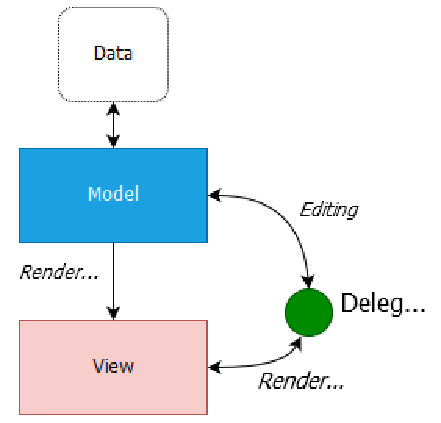
\includegraphics[width=0.4\textwidth,keepaspectratio]{Model_View_architecture.pdf}
%  & 模型/视图架构 模型与数据源通信,为架构中的其他组件提供接口。通信的性质取决于数据源的类型以及模型的实现方式。
%
%
%视图从模型中获取模型索引; 这些索引是对数据项的引用。 通过向模型提供模型索引,视图可以从数据源检索出数据项。
%
%
%在标准视图中,委托负责渲染显示数据项。 当编辑项目后,委托将直接通过模型索引与模型进行通信。\\
%
%\hline	
%\end{tabular}


\begin{tabular}{|l|m{25em}|}
\hline
   
    
    \adjustbox{valign=t}{ 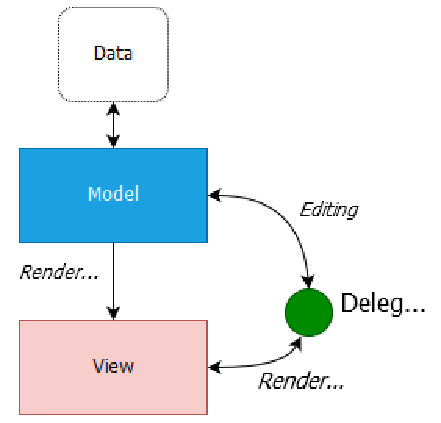
\includegraphics[width=0.4\textwidth]{Model_View_architecture.pdf}}
  & 模型/视图架构 模型与数据源通信,为架构中的其他组件提供接口。通信的性质取决于数据源的类型以及模型的实现方式。


视图从模型中获取模型索引; 这些索引是对数据项的引用。 通过向模型提供模型索引,视图可以从数据源检索出数据项。


在标准视图中,委托负责渲染显示数据项。 当编辑项目后,委托将直接通过模型索引与模型进行通信。\\

\hline	
\end{tabular}


通常,模型/视图类可以分为上述三个组:模型,视图和委托。这些组件中的每个组件都由抽象类定义,这些抽象类提供了公共接口,并在某些情况下提供了一些功能的默认实现。抽象类应被子类化,以提供其他组件期望的全部功能;当然也可以编写专用组件。

模型、视图和委托之间通过信号槽通信。

\begin{compactitem}
	\item 数据源的数据发生改变时模型将发射信号通知视图。
\item 用户交互发生改变时,视图将发射相应的信号。
\item 在编辑期间,委托将发射信号来告知模型和视图有关编辑器的状态。
\end{compactitem}


\section{模型}

所有项目模型均基于 QAbstractItemModel 类。此类定义一个接口,视图和委托使用该接口访问数据。数据本身不必存储在模型中。它可以保存在由单独的类,文件,数据库或某些其他应用程序组件提供的数据结构或存储库中。


有关模型的基本概念在 “模型类”部分中介绍。


QAbstractItemModel 提供了一个数据接口,该接口足够灵活,可以处理以表,列表和树的形式表示数据的视图。但是,当为列表和类似表的数据结构实现新模型时,QAbstractListModel 和 QAbstractTableModel 类是更好的选择,因为它们提供了常用功能的默认实现。这些类中的每一个都可以被子类化以提供支持特殊类型的列表和表的模型。


在 创建新模型 部分中讨论了模型子类化的过程。


Qt提供了一些现成的模型,可用于处理数据项:

\begin{compactitem}
\item QStringListModel 用于存储一列简单的 QString 类型的项目。
\item QStandardItemModel 用于管理更复杂的树形结构项目,每个项目可以包含任意数据。
\item QFileSystemModel 提供有关本地归档系统中文件和目录的信息。
\item QSqlQueryModel,QSqlTableModel 和 QSqlRelationalTableModel 用于在使用模型/视图架构时访问数据库。
\end{compactitem}


如果这些标准模型不满足您的要求,则可以将 QAbstractItemModel,QAbstractListModel 或 QAbstractTableModel 子类化以创建您自己的自定义模型。

\section{视图}

Qt 提供了针对各种视图的完整实现:QListView 用于显示项目列表,QTableView 用于显示表结构模型的数据,QTreeView 在一个分层次的结构列表中显示数据项。这些类均基于 QAbstractItemView 抽象基类。尽管这些类都是已经实现好的,但也可以将它们子类化以提供满足我们需求的自定义视图。


所有可用的视图可在 视图类 部分中进行查阅。

\section{委托}

QAbstractItemDelegate 是模型/视图框架中委托的抽象基类。默认委托实现由 QStyledItemDelegate 提供, Qt 中的标准视图都将其作为默认委托。但是,QStyledItemDelegate 和 QItemDelegate 是绘制和为视图中的项目提供编辑器的独立替代方法。它们之间的区别在于 QStyledItemDelegate 使用当前样式来绘制其项目。因此,在实现自定义委托或使用 Qt 样式表时,建议将 QStyledItemDelegate 用作基类。


委托在 “委托类” 部分中进行了描述。

\section{排序}

在模型/视图架构中,有两种方法可以进行排序;选择哪种方法取决于底层使用的模型。


如果您的模型是可排序的,即重新实现 QAbstractItemModel::sort() 函数,则 QTableView 和 QTreeView 都提供了API,可让您以编程方式对模型数据进行排序。 另外,通过将 QHeaderView::sortIndicatorChanged() 信号连接到 QTableView::sortByColumn() 槽函数或 QTreeView::sortByColumn() 槽函数,可以启用交互式排序(即允许用户通过单击视图的标题对数据进行排序))。


如果您的模型没有所需的接口,或者如果您想使用列表视图来呈现数据,则另一种方法是在视图呈现数据之前,使用委托模型来转换模型的结构。 有关 代理模型 的部分将对此进行详细介绍。

\section{便捷类}

从标准视图类派生出了许多便捷类,用于 Qt 中基于项目的项目视图类和表类,它们不打算被子类化。

比如 QListWidget,QTreeWidget 和 QTableWidget。

这些类的灵活性不如视图类,并且不能与任意模型一起使用。我们建议您使用模型/视图方法来处理项目视图中的数据,除非您强烈需要一组基于项目的类。

如果希望在使用基于项目的接口的同时利用模型/视图方法提供的功能,请考虑将视图类(例如 QListView,QTableView 和 QTreeView )与 QStandardItemModel 一起使用。

\section{使用模型和视图}

以下各节说明如何在 Qt 中使用模型/视图模型。每个部分都包含一个示例,紧接着是展示如何创建新组件。

\subsection{Qt 中包含的两个模型}

Qt 提供的两个标准模型是 QStandardItemModel 和 QFileSystemModel。QStandardItemModel 是一个多功能模型,可用于表示列表,表和树视图所需的各种不同的数据结构。该模型还保存数据项。QFileSystemModel 是用于维护有关目录内容的信息的模型,它本身不保存任何数据项,而仅表示本地文件系统上的文件和目录。

QFileSystemModel 提供了一个现成的模型用来测试使用,并且可以通过简单的配置就可以使用现有的数据。使用该模型,我们可以展示如何创建一个可用于现成视图的模型,并探索如何使用模型索引来操控数据。

\subsection{通过现有模型使用视图}

QListView 和 QTreeView 类是最适合与 QFileSystemModel一起使用的视图。下面提供的示例是分别在树形视图和列表视图中显示相同的目录内容。这些视图共享用户的选择,以便在两个视图中突出显示所选的项目。

\begin{figure}[hpt!]  
	\centering
    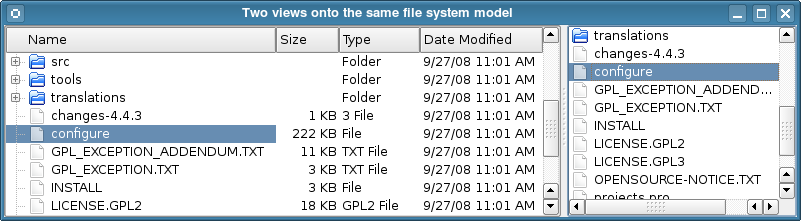
\includegraphics[width=0.5\textwidth]{shareddirmodel}
\end{figure}

我们使用了现成的模型 QFileSystemModel,并创建了一些视图来显示目录的内容。展示了使用模型的最简单方法。 该模型的构建和使用是在单个 main() 函数中执行的:

\begin{lstlisting}[language=C++]
int main(int argc, char *argv[])
{
    QApplication app(argc, argv);
    QSplitter *splitter = new QSplitter;

    QFileSystemModel *model = new QFileSystemModel;
    model->setRootPath(QDir::currentPath());
\end{lstlisting}

该模型被设置为使用来自特定文件系统的数据。调用 setRootPath() 将告诉模型文件系统上的哪个驱动器会暴露给视图。

我们使用同一个模型创建两个不同的视图,来查看模型中的项目呈现出来的效果:

\begin{lstlisting}[language=C++]
QTreeView *tree = new QTreeView(splitter);
tree->setModel(model);
tree->setRootIndex(model->index(QDir::currentPath()));

QListView *list = new QListView(splitter);
list->setModel(model);
list->setRootIndex(model->index(QDir::currentPath()));
\end{lstlisting}

视图的构造方法与其他部件一样。设置视图来显示模型中的项目仅需使用目录模型作为参数来调用视图的 setModel() 函数即可。我们通过在每个视图上调用 setRootIndex() 函数来过滤模型提供的数据,并从文件系统模型中为当前目录传递合适的模型索引。

这种情况下对于 QFileSystemModel 来说只能通过传递一个目录参数来使用 index() 函数获取索引,模型索引在 模型类 部分中讨论。

该函数的其余部分是在分裂器部件中显示视图,并运行应用程序的事件循环:

\begin{lstlisting}[language=C++]
    splitter->setWindowTitle("Two views onto the same file system model");
    splitter->show();
    return app.exec();
}
\end{lstlisting}

在上面的示例中,我们忽略了如何处理项目选择。 在 处理项目视图中的选择项 部分中将更详细地介绍。

\section{模型类}

在学习如何处理选择项之前,理解模型/视图框架中使用的概念是很有用的。

\subsection{基本概念}

在模型/视图体系结构中,模型提供了视图和委托用来访问数据的标准接口。在 Qt 中,标准接口由 QAbstractItemModel 类定义。无论数据项如何存储在任何基础数据结构中,QAbstractItemModel 的所有子类都将数据表示为一个有层次的包含项表的结构。视图使用此约定来访问模型中的数据项,但是它们向用户呈现此信息的方式不受限制。

\begin{figure}[hpt!]  
	\centering
    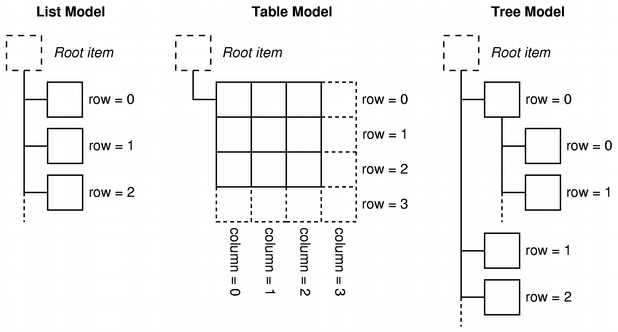
\includegraphics[width=0.5\textwidth]{modelview-models}
\end{figure}

模型通过信号槽机制通知所有附加视图有关数据更改的信息。

本节描述一些基本概念,这些概念对于其他组件通过模型类访问数据项的方式至关重要。 稍后的部分将讨论更高级的概念。

\section{模型索引}

为了确保数据的表示方式与访问方式分开,引入了模型索引的概念。通过模型获得的每条信息都由模型索引表示。视图和委托使用这些索引来请求要显示的数据项。

所以,只有模型需要知道如何获取数据和定义数据类型。模型索引包含一个指向创建它们的模型的指针,以免在使用多个模型时造成混淆。

\begin{lstlisting}[language=C++]
QAbstractItemModel *model = index.model();
\end{lstlisting}

模型索引提供了一个对信息的临时的引用,可用于通过模型检索或修改数据。由于模型可能会不时重组其内部结构,因此模型索引可能会变得无效,不应进行存储。如果需要长期使用一条信息,则必须创建一个持久的模型索引。这为模型保持最新状态提供了参考。临时模型索引由 QModelIndex 类提供,而持久模型索引由 QPersistentModelIndex 类提供。

要获得与数据项相对应的模型索引,必须为模型指定三个属性:行号,列号和父项的模型索引。以下各节将详细描述和解释这些属性。

\section{行和列}

在基本的形式中,可以将模型作为一个简单的表进行访问,项目按行和列的编号位于其中。

这并不意味着底层数据存储在数组结构中;行号和列号的使用仅仅是组件之间相互通信的约定。

我们可以通过在模型中指定给定项目的行号和列号来检索有关任何给定项目的信息,我们接收到的是代表该项目的索引:

\begin{lstlisting}[language=C++]
QModelIndex index = model->index(row, column, ...);
\end{lstlisting}


为简单的单层数据结构(例如列表和表)提供接口的模型不需要提供任何其他信息,但是,如上述代码所示,在获取模型索引时,我们需要提供更多信息。

\begin{tabular}{|l|m{25em}|}
\hline
\adjustbox{valign=t}{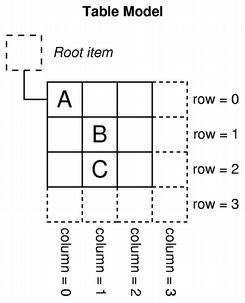
\includegraphics[width=0.5\textwidth]{modelview-tablemodel}}
  & 
  行和列
  
该图显示了基本表模型的表示形式,其中每个项目都由一对行号和列号定位。通过将相关的行号和列号传递给模型,我们获得了一个引用数据项的模型索引。

\begin{lstlisting}[language=C++]
QModelIndex indexA = model->index(0, 0, QModelIndex());
QModelIndex indexB = model->index(1, 1, QModelIndex());
QModelIndex indexC = model->index(2, 1, QModelIndex());
\end{lstlisting}

始终通过用 QModelIndex() 指定为其父项来引用模型中的顶级项目。下一节将对此进行讨论。\\
\hline	
\end{tabular}

\section{项的父项}
当在表视图或列表视图中使用数据时,模型提供的类似于表的接口就非常合适。行号和列号系统准确地映射到视图显示项目的方式上。但是,诸如树状视图的结构对于模型项目的操作要求模型提供更灵活的接口。每个项目也可以是另一个项目表的父项,就像树状视图中的顶级项目可以包含另一个项目列表一样。

当请求模型项的索引时,我们必须提供有关该项父项的一些信息。在模型之外,引用项目的唯一方法是通过模型索引,因此还必须提供父模型索引:

\begin{lstlisting}[language=C++]
QModelIndex index = model->index(row, column, parent);
\end{lstlisting}

\begin{tabular}{|l|m{25em}|}
\hline
    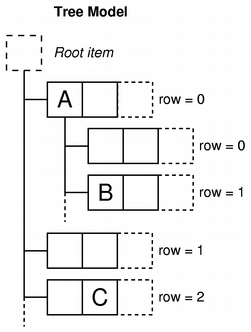
\includegraphics[width=0.5\textwidth]{modelview-treemodel}
  & 
父项、行和列

该图展示了树模型的表示形式,其中每一项均由父项、行号和列号检索出来。

“A”和“C”项在模型中为同级顶级:

\begin{lstlisting}[language=C++]
QModelIndex indexA = model->index(0, 0, QModelIndex());
QModelIndex indexC = model->index(2, 1, QModelIndex());
\end{lstlisting}

“A”项有多个子项。使用以下代码获得“B”项的模型索引:

\begin{lstlisting}[language=C++]
QModelIndex indexB = model->index(1, 0, indexA);
\end{lstlisting}
\\
\hline	
\end{tabular}

\section{项角色}

模型中的项可以为其他组件扮演各种不同的角色,从而可以为不同的数据提供不同的方案。 例如,Qt::DisplayRole 用于访问可以在视图中显示为文本的字符串。通常,项包含许多不同角色的数据,标准角色由 Qt::ItemDataRole 定义。

我们可以通过向模型传递与该项相对应的模型索引,并指定一个角色来获取所需的数据类型,从而获得我们想要的数据:

\begin{lstlisting}[language=C++]
QVariant value = model->data(index, role);
\end{lstlisting}


\begin{tabular}{|l|m{25em}|}
\hline
    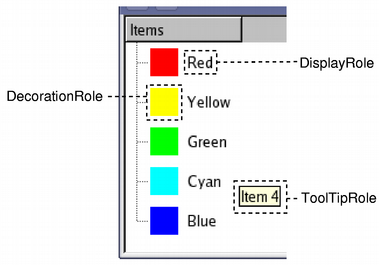
\includegraphics[width=0.5\textwidth]{modelview-roles}
  & 
项角色

项角色向模型指示要引用的数据类型。视图可以以不同的方式显示角色,因此为每个角色提供适当的信息很重要。

创建新模型 部分将更详细地介绍角色的某些特定用法。\\
\hline	
\end{tabular}


项标准角色 Qt::ItemDataRole 涵盖了大部分常用的项角色。通过为每个角色提供适当的项目数据,模型可以向视图和委托提示如何将项呈现给用户。不同类型的视图可以根据自身需要解释或忽略此信息。也可以为特定目的定义其他角色。

\section{摘要}

\begin{compactitem}
\item 模型索引以独立于任何底层数据结构的方式提供给视图和委托有关模型所提供项的位置的信息。
\item 项通过其行号和列号以及其父项的模型索引检索出来。
\item 模型索引是由模型根据其他组件(例如视图和委托)的请求构造出来的。
\item 如果使用 index() 请求索引时为父项指定了有效的模型索引,则返回的索引将引用模型中该父项之下的项。获得的索引指向该项目的子项。
\item 如果使用 index() 请求索引时为父项指定了无效的模型索引,则返回的索引引用模型中的顶级项。
\item 项角色 用来区分与项关联的不同类型的数据。
\end{compactitem}

\section{使用模型索引}

为了演示如何使用模型索引从模型中检索数据,我们设置了一个没有视图的 QFileSystemModel,并在部件中显示文件和目录的名称。尽管这没有展示使用模型的正常方法,但是它说明了在处理模型索引时模型使用的规则。

QFileSystemModel 加载是异步的,以最大程度地减少系统资源的使用。在处理此模型时,我们必须考虑到这一点。

我们通过以下方式构造文件系统模型:

\begin{lstlisting}[language=C++]
QFileSystemModel *model = new QFileSystemModel;
connect(model, &QFileSystemModel::directoryLoaded, [model](const QString &directory) {
    QModelIndex parentIndex = model->index(directory);
    int numRows = model->rowCount(parentIndex);
});
model->setRootPath(QDir::currentPath);
\end{lstlisting}

在这种情况下,我们首先设置默认的 QFileSystemModel 。我们将其连接到 \hl{lambda},在其中我们将使用该模型提供的 index() 的特定实现来获取父索引。 在 \hl{lambda} 中,我们使用 rowCount() 函数计算模型中的行数。最后,我们设 QFileSystemModel 的根路径,以便它开始加载数据并触发 \hl{lambda} 。

为简单起见,我们只处理模型第一栏中的项目。我们依次检查每一行,获取每一行中第一项的模型索引,然后读取模型中为该项存储的数据。

\begin{lstlisting}[language=C++]
for (int row = 0; row < numRows; ++row) {
    QModelIndex index = model->index(row, 0, parentIndex);
\end{lstlisting}

为了获得模型索引,我们指定行号,列号(第一列为零),并为所需的所有项的父项指定适当的模型索引。使用模型的 data() 函数检索存储在每个项目中的文本。我们指定模型索引和 DisplayRole 获取字符串形式的项数据。

\begin{lstlisting}[language=C++]
QString text = model->data(index, Qt::DisplayRole).toString();
    // Display the text in a widget.

}
\end{lstlisting}

以上示例演示了从模型中检索数据的基本用法:

\begin{compactitem}
\item 模型的大小范围可以使用 rowCount() 和 columnCount 获取到。这些函数通常需要指定一个父项模型索引。
\item 模型索引用于访问模型中的数据项。指定一个项需要行、列和父项的模型索引。
\item 通过 \hl{QModelIndex()} 指定一个空的父项的索引来访问模型中的顶层项。
\item 项包含不同角色的数据。要获得特定角色的数据,必须同时向模型提供模型索引和角色。
\end{compactitem}


\subsection{拓展阅读}

可以通过提供了标准接口的 QAbstractItemModel 类来创建新模型。在 创建新模型 部分,我们将通过创建一个方便可用的保存字符串列表的模型来展示这一点。

\section{视图类}
\subsection{概念}

在模型/视图架构中,视图从模型中获取数据项并将其呈现给用户。呈现数据的方式不必类似于模型提供数据的方式,而可以与用于存储数据项的底层数据结构完全不同。

通过使用 QAbstractItemModel 提供的标准模型接口,QAbstractItemView 提供的标准视图接口以及使用表示数据项的模型索引来实现内容和表示的分离。视图通常管理从模型获得的数据的整体布局。它们可以自己呈现单个数据项,或使用委托来处理渲染和编辑功能。

除了显示数据外,视图还处理项目之间的导航以及项目选择。这些视图还实现了基本的用户界面功能,例如上下文菜单和拖放功能。视图可以提供项目的默认编辑功能,也可以与 委托 一起使用以提供自定义编辑器。

可以在没有模型的情况下构造视图,但是必须提供模型才能显示有用的信息。视图通过使用 选择项 来跟踪用户选择的项目,这些选择项可以被每个视图单独维护,或者在多个视图之间共享。

一些视图,例如 QTableView 和 QTreeView,需要显示表头和项目。这些由视图类 QHeaderView 实现。表头通常与包含它们的视图访问的是同一个模型。他们使用 QAbstractItemModel::headerData() 函数从模型中检索数据,并且通常以标签形式显示表头信息。可以继承 QHeaderView 类实现新的标头,以为视图提供更专业的标签。


\chapter{模型视图教程}

每个 \hl{UI} 开发人员都应该了解模型视图编程,本教程的目的是让您轻松理解有关模型视图的相关知识。

表格,列表和树部件是 GUI 中经常使用的组件。这些部件可以通过两种不同的方式访问其数据。
传统方式是,这些部件包含用于存储数据的内部容器。这种方法非常直观,但是,在许多应用程序中,它会导致数据同步问题。
第二种方法是模型/视图编程,其中部件不维护内部数据容器。他们通过标准化接口访问外部数据,因此避免了数据重复。
乍一看,这似乎很复杂,但是如果您仔细看一看,不仅容易掌握,而且模型/视图编程的许多好处也变得更加明显。

\begin{figure}[hbt!]  
	% \centering
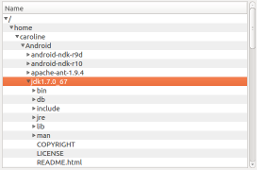
\includegraphics[width=0.3\textwidth]{treeview}
\end{figure}

在此过程中,我们将了解 \hl{Qt} 提供的一些基本技术,例如:

\begin{compactitem}
\item 标准部件和模型视图部件的区别
\item 窗体和模型之间的适配器
\item 开发一个简单的模型视图的应用程序
\item 预定义模型
\item 中间主题,比如:
\begin{compactitem}
\item 树形视图
\item 选项
\item 委托
\item 模型调试测试
\end{compactitem}
\end{compactitem}

您还将了解到新的应用程序是否可以通过模型/视图编程更容易地编写,或者经典的标准部件是否也可以工作。

本教程中的代码您可以编辑修改或者集成到您的项目中去。 
源码在 \hl{Qt} 的 \hl{examples/widgets/tutorials/modelview} 目录。

详见 参考文档

\section{介绍}

模型/视图是一种将数据从视图中分离出来,来处理数据集的一种技术。标准部件并不是为将数据从视图中分离出来而设计的,这就是为什么 Qt 会有两种不同类型的部件。
这两种部件看起来都一样,但是它们与数据之间的交互方式是不同的。

\begin{longtable}[l]{|l|m{25em}|}
\hline
标准部件使用的数据最为部件的一部分。\\
&
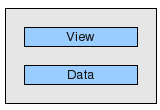
\includegraphics[width=0.4\textwidth]{standardwidget} \\ 
\hline	
视图类操作的是外部的数据(模型)。\\
&
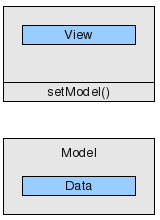
\includegraphics[width=0.4\textwidth]{modelview} \\ 
\hline	
\end{longtable}

\subsection{标准部件}

让我们仔细看一下标准表部件。表格部件是用户可以更改的数据元素的 2D 数组。
通过读取和写入表部件提供的数据元素,可以将表部件集成到程序流中。
该方法非常直观,在许多应用程序中很有用,但是使用标准表窗口部件显示和编辑数据库表可能会出现问题。
数据的两个副本必须协调一致:一个在部件外部;另一个在部件外部。开发人员负责同步两个版本。
除此之外,表示和数据的紧密耦合使编写单元测试更加困难。

\subsection{使用模型/视图解决}

模型/视图提供了一个使用更通用体系结构的解决方案。
模型/视图消除了标准控件可能出现的数据一致性问题。
模型/视图还可以更容易地使用同一数据的多个视图,因为一个模型可以传递给多个视图。
最重要的区别是模型/视图部件不在表单元格后面存储数据。实际上,它们直接根据您的数据进行操作。
因为视图类不知道数据的结构,所以需要提供一个包装器,使数据符合 QAbstractItemModel 接口。
视图使用此接口读取和写入数据。实现 QAbstractItemModel 类的任何实例都称为模型。
一旦视图接收到指向模型的指针,它将读取和显示其内容,并成为其编辑器。

\subsection{模型/视图部件概览}

下面是模型/视图部件及其对应的标准部件。

\begin{longtable}[l]{|l|m{15em}|m{10em}|}
\hline
部件 & 标准部件 (基于项的便捷类) & 模型/视图 视图类 (使用外部数据) \\ 
\hline
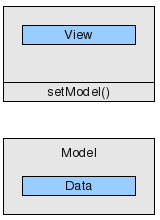
\includegraphics[width=0.4\textwidth]{modelview}  
&
QListWidget
&
QListView  \\
\hline
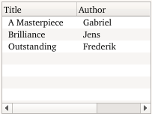
\includegraphics[width=0.4\textwidth]{tableview}  
&
QTableWidget	
&
QTableView \\
\hline
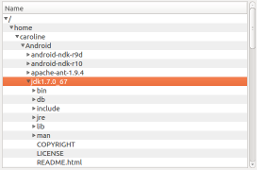
\includegraphics[width=0.4\textwidth]{treeview}  
&
QTreeWidget	
&
QTreeView  \\
\hline
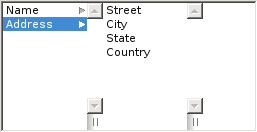
\includegraphics[width=0.4\textwidth]{columnview}  
&

&
QColumnView s显示列表层次结构的树视图  \\
\hline
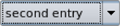
\includegraphics[width=0.4\textwidth]{modelview-combobox}  
&
QComboBox 既可以用作视图类,也可以用作传统部件
&
  \\
\hline
\end{longtable}



\subsection{在表单和模型之间使用适配器}

在表单和模型之间使用适配器非常方便。
我们可以直接从表内部编辑存储在表中的数据,但是在文本字段中编辑数据更为方便。
在对部件的一个数据而不是数据集操作时,模型/视图并没有提供对应的方法将数据和视图分离开。
比如 QLineEdit,QCheckBox...因此我们需要一个适配器来将表单连接到数据源。

QDataWidgetMapper 是一个很好的解决方案,因为它可以将表单部件映射到表行,并且为数据库表构建表单非常容易。

\begin{figure}[hbt!]  
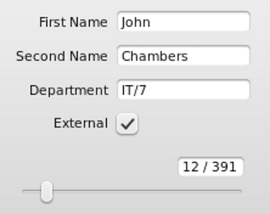
\includegraphics[width=0.3\textwidth]{widgetmapper}
\end{figure}

适配器的另一个例子是 QCompleter。
Qt 使用 QCompleter 在 Qt 部件(如 QComboBox 和 如下图所示的 QLineEdit)中提供自动补全功能。
QCompleter使用模型作为其数据源。
	
\begin{figure}[hbt!]  
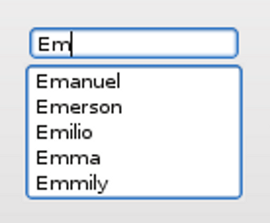
\includegraphics[width=0.3\textwidth]{qcompleter}
\end{figure}

\section{一个简单的模型/视图应用程序}

如果要开发模型/视图应用程序,应该从哪里开始?我们建议从一个简单的示例开始,并逐步扩展它。
这样更容易理解模型/视图架构。
事实证明,在调用 IDE 之前尝试详细了解模型/视图体系结构对于许多开发人员来说并不方便。
从具有演示数据的简单模型/视图应用程序开始要容易得多。
试试看!只需将以下示例中的数据替换为您自己的数据即可。

以下是7个非常简单和独立的应用程序,它们展示了模型/视图编程的不同方面。
可以在 examples/widgets/tutorials/modelview 目录中找到源代码。

\subsection{只读的表}

我们从使用 QTableView 来显示数据的应用程序开始。稍后我们将添加编辑功能。
(文件: examples/widgets/tutorials/modelview/1\_readonly/main.cpp)

\begin{cppcode}
// main.cpp
#include <QApplication>
#include <QTableView>
#include "mymodel.h"
	
int main(int argc, char *argv[])
{
	QApplication a(argc, argv);
	QTableView tableView;
	MyModel myModel;
	tableView.setModel(&myModel);
	tableView.show();
	return a.exec();
}
\end{cppcode}

main() 函数:

这是有趣的部分:我们创建 MyModel 的实例并使用 tableView.setModel(&myModel);。 
将其指针传递给 tableView。 tableView 将调用它收到的指针的方法来找出两件事:

\begin{compactitem}
\item 需要显示多少行和列。
\item 每个单元格中应该显示什么内容。
\end{compactitem}

模型需要一些代码来响应以上这些。

我们有一个表数据集,因此让我们从 QAbstractTableModel 开始,因为它比更通用的 QAbstractItemModel 更易于使用。

(文件:examples/widgets/tutorials/modelview/1\_readonly/mymodel.h)

\begin{cppcode}
// mymodel.h
#include <QAbstractTableModel>
	
class MyModel : public QAbstractTableModel
{
	Q_OBJECT
public:
	MyModel(QObject *parent = nullptr);
	int rowCount(const QModelIndex &parent = QModelIndex()) const override;
	int columnCount(const QModelIndex &parent = QModelIndex()) const override;
	QVariant data(const QModelIndex &index, int role = Qt::DisplayRole) const override;
};
\end{cppcode}

QAbstractTableModel 需要实现三个抽象方法。

(文件:\hl{examples/widgets/tutorials/modelview/1\_readonly/mymodel.cpp})

\begin{cppcode}
	// mymodel.cpp
#include "mymodel.h"

MyModel::MyModel(QObject *parent)
    : QAbstractTableModel(parent)
{
}

int MyModel::rowCount(const QModelIndex & /*parent*/) const
{
   return 2;
}

int MyModel::columnCount(const QModelIndex & /*parent*/) const
{
    return 3;
}

QVariant MyModel::data(const QModelIndex &index, int role) const
{
    if (role == Qt::DisplayRole)
       return QString("Row%1, Column%2")
                   .arg(index.row() + 1)
                   .arg(index.column() +1);

    return QVariant();
}
\end{cppcode}


行数和列数由 MyModel::rowCount() 和 MyModel::columnCount() 提供。
当视图必须知道单元格的文本是什么时,它将调用方法 MyModel::data()。
行和列信息由参数 index 指定,并且角色设置为 Qt::DisplayRole。
下一节将介绍其他角色。在我们的示例中,生成了应显示的数据。
在实际的应用程序中,MyModel 会有一个名为 MyData 的成员,该成员充当所有读取和写入操作的目标。

这个小例子说明了模型的被动性质。该模型不知道何时使用它或需要哪些数据。
每次视图请求时,它仅提供数据。

当需要更改模型数据时会发生什么?视图如何认识到数据已更改并且需要再次读取?
该模型必须发射一个信号,该信号指示已更改了哪些单元格范围。这将在第2.3节中演示。

\subsection{使用角色扩展只读表格示例}

除了控制视图显示的文本之外,模型还控制文本的外观。
当我们稍微改变模型时,我们得到以下结果:

\begin{figure}[hbt!]  
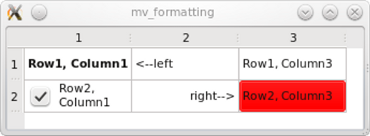
\includegraphics[width=0.5\textwidth]{readonlytable_role}
\end{figure}

实际上,除了 data() 方法外,无需更改其他任何内容即可设置字体,背景色,对齐方式和复选框。
下面是产生上面所示结果的 data() 方法。不同之处在于,这次我们使用参数 int 角色根据其值返回不同的信息。

(文件: examples/widgets/tutorials/modelview/2\_formatting/mymodel.cpp)

\begin{cppcode}
// mymodel.cpp
QVariant MyModel::data(const QModelIndex &index, int role) const
{
    int row = index.row();
    int col = index.column();
    // generate a log message when this method gets called
    qDebug() << QString("row %1, col%2, role %3")
            .arg(row).arg(col).arg(role);

    switch (role) {
    case Qt::DisplayRole:
        if (row == 0 && col == 1) return QString("<--left");
        if (row == 1 && col == 1) return QString("right-->");

        return QString("Row%1, Column%2")
                .arg(row + 1)
                .arg(col +1);
    case Qt::FontRole:
        if (row == 0 && col == 0) { //change font only for cell(0,0)
            QFont boldFont;
            boldFont.setBold(true);
            return boldFont;
        }
        break;
    case Qt::BackgroundRole:
        if (row == 1 && col == 2)  //change background only for cell(1,2)
            return QBrush(Qt::red);
        break;
    case Qt::TextAlignmentRole:
        if (row == 1 && col == 1) //change text alignment only for cell(1,1)
            return Qt::AlignRight + Qt::AlignVCenter;
        break;
    case Qt::CheckStateRole:
        if (row == 1 && col == 0) //add a checkbox to cell(1,0)
            return Qt::Checked;
        break;
    }
    return QVariant();
}
\end{cppcode}

每个格式化属性将通过对 data() 方法的单独调用从模型中请求。
角色参数用于让模型知道请求哪个属性:

\begin{tabular}{|l|m{15em}|l|}
	\hline
	枚举 enum Qt::ItemDataRole & 意义 &类型 \\
	\hline
	Qt::DisplayRole	 & 文本	 &QString \\
	\hline
	Qt::FontRole	& 字体	&QFont\\ 
	\hline
	BackgroundRole &	单元格背景的画笔	& QBrush\\ 
	\hline
	Qt::TextAlignmentRole	& 文本对齐方式 &enum Qt::AlignmentFlag \\
	\hline 
	Qt::CheckStateRole &	使用 QVariant() 取消复选框,使用 Qt::Checked 或 Qt::UnChecked 设置复选框 &	enum Qt::ItemDataRole \\
	\hline
\end{tabular}

请参阅 Qt 明明控件文档了解有关 Qt::ItemDataRole 枚举功能的更多信息。

现在我们需要确定使用分离的模型如何影响应用程序的性能,因此让我们跟踪视图调用 data() 方法的频率。
为了跟踪视图调用模型的频率,我们在 data() 方法中放置了一条调试语句,该语句记录到错误输出流中。
在我们的小示例中,data() 将被调用 42 次。
每次将光标悬停在该字段上时,都会再次调用 data(),每个单元格7次。
这就是为什么在调用 data() 和缓存昂贵的查找操作时确保数据可用的重要原因。

\subsection{表内的时钟}

\begin{figure}[hbt!]  
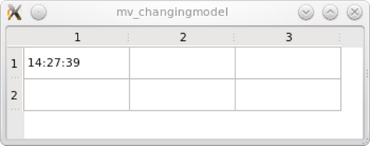
\includegraphics[width=0.5\textwidth]{img/clock}
\end{figure}

我们仍然使用一个只读表,但是这次内容每秒更改一次,因为我们正在显示当前时间。

(文件:examples/widgets/tutorials/modelview/3\_changingmodel/mymodel.cpp)

\begin{cppcode}
QVariant MyModel::data(const QModelIndex &index, int role) const
{
    int row = index.row();
    int col = index.column();

    if (role == Qt::DisplayRole && row == 0 && col == 0)
        return QTime::currentTime().toString();

    return QVariant();
}
\end{cppcode}

缺少一些东西来使时钟滴答作响。我们需要每秒告诉视图时间已更改,并且需要再次读取。
我们用一个计时器来做到这一点。
在构造函数中,我们将其间隔设置为1秒,然后连接其超时信号。

(文件:examples/widgets/tutorials/modelview/3\_changingmodel/mymodel.cpp)

\begin{cppcode}
MyModel::MyModel(QObject *parent)
    : QAbstractTableModel(parent)
    , timer(new QTimer(this))
{
    timer->setInterval(1000);
    connect(timer, &QTimer::timeout , this, &MyModel::timerHit);
    timer->start();
}
\end{cppcode}

(文件:examples/widgets/tutorials/modelview/3\_changingmodel/mymodel.cpp)

槽函数:

\begin{cppcode}
void MyModel::timerHit()
{
    //we identify the top left cell
    QModelIndex topLeft = createIndex(0,0);
    //emit a signal to make the view reread identified data
    emit dataChanged(topLeft, topLeft, {Qt::DisplayRole});
}
\end{cppcode}

我们通过发射 dataChanged() 信号要求视图再次读取左上角单元格中的数据。
请注意,我们没有将 dataChanged 信号显式连接到视图。这在我们调用 setModel 时自动发生。

\subsection{设置行和列的标题} 

标题可以通过调用视图的一个方法被隐藏: tableView->verticalHeader()->hide();

\begin{figure}[hbt!]  
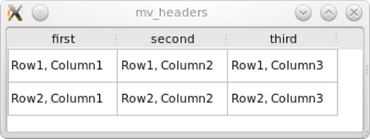
\includegraphics[width=0.5\textwidth]{modelview-header}
\end{figure}

但是,标题内容是通过模型设置的,因此我们重新实现 headerData() 方法:

(文件:examples/widgets/tutorials/modelview/4\_headers/mymodel.cpp)

\begin{cppcode}
QVariant MyModel::headerData(int section, Qt::Orientation orientation, int role) const
{
    if (role == Qt::DisplayRole && orientation == Qt::Horizontal) {
        switch (section) {
        case 0:
            return QString("first");
        case 1:
            return QString("second");
        case 2:
            return QString("third");
        }
    }
    return QVariant();
}
\end{cppcode}

\begin{lstlisting}
方法 headerData() 也具有角色参数,该角色与 MyModel::data() 中的含义相同。
\end{lstlisting}

\subsection{最小编辑示例}

在此示例中,我们将构建一个应用程序,该应用程序通过重复输入表单元格中的值来自动用内容填充窗口标题。为了能够轻松访问窗口标题,我们将 QTableView 放在 QMainWindow 中。

该模型决定编辑功能是否可用。我们仅需修改模型即可启用可用的编辑功能。这可以通过重新实现以下虚函数来完成:setData() 和 flags()。

(文件:examples/widgets/tutorials/modelview/5\_edit/mymodel.h)


\begin{cppcode}
// mymodel.h
#include <QAbstractTableModel>
#include <QString>

const int COLS= 3;
const int ROWS= 2;

class MyModel : public QAbstractTableModel
{
    Q_OBJECT
public:
    MyModel(QObject *parent = nullptr);
    int rowCount(const QModelIndex &parent = QModelIndex()) const override;
    int columnCount(const QModelIndex &parent = QModelIndex()) const override;
    QVariant data(const QModelIndex &index, int role = Qt::DisplayRole) const override;
    bool setData(const QModelIndex &index, const QVariant &value, int role = Qt::EditRole) override;
    Qt::ItemFlags flags(const QModelIndex &index) const override;
private:
    QString m_gridData[ROWS][COLS];  //holds text entered into QTableView
signals:
    void editCompleted(const QString &);
};
\end{cppcode}

我们使用二维数组 QString m\_gridData 来存储我们的数据。这使 m\_gridData 成为 MyModel 的核心。
MyModel 的其余部分就像包装器一样,将 m\_gridData 调整为 QAbstractItemModel 接口。
我们还引入了 editCompleted() 信号,这使得将修改后的文本传输到窗口标题成为可能。

(文件:examples/widgets/tutorials/modelview/5\_edit/mymodel.cpp)

\begin{cppcode}
bool MyModel::setData(const QModelIndex &index, const QVariant &value, int role)
{
    if (role == Qt::EditRole) {
        if (!checkIndex(index))
            return false;
        //save value from editor to member m_gridData
        m_gridData[index.row()][index.column()] = value.toString();
        //for presentation purposes only: build and emit a joined string
        QString result;
        for (int row = 0; row < ROWS; row++) {
            for (int col= 0; col < COLS; col++)
                result += m_gridData[row][col] + ' ';
        }
        emit editCompleted(result);
        return true;
    }
    return false;
}
\end{cppcode}
    
每次用户编辑单元格时都会调用 setData() 。index 参数告诉我们哪个字段已被编辑,value 提供了编辑过程的结果。
该角色将始终设置为 Qt::EditRole,因为我们的单元格仅包含文本。
如果存在一个复选框,并且将用户权限设置为允许选中该复选框,则还将以角色设置为 Qt::CheckStateRole 进行调用。

(文件:\hl{examples/widgets/tutorials/modelview/5\_edit/mymodel.cpp})

\begin{cppcode}
Qt::ItemFlags MyModel::flags(const QModelIndex &index) const
{
    return Qt::ItemIsEditable | QAbstractTableModel::flags(index);
}
\end{cppcode}

单元格的各种属性可以使用 flags() 进行调整。

返回 Qt::ItemIsSelectable | Qt::ItemIsEditable | Qt::ItemIsEnabled 足以显示一个可被单元格选中的编辑器。

如果编辑一个单元格所修改的数据多于该特定单元格中的数据,则该模型必须发射 dataChanged() 信号,以便读取已更改的数据。

\section{中间主题}

\subsection{树视图}

您可以将上面的示例转换为具有树视图的应用程序。
只需将 QTableView 替换为 QTreeView,这将生成一个读/写树。不必对模型进行任何更改。
树不会有任何层次结构,因为模型本身没有任何层次结构。

\begin{figure}[hbt!]  
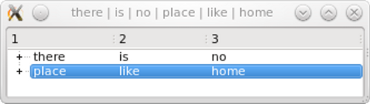
\includegraphics[width=0.5\textwidth]{dummy_tree}
\end{figure}


QListView,QTableView 和 QTreeView 均使用了合并了列表、表和树的模型抽象。
这样就可以让不同类型的视图类使用同一模型。

\begin{figure}[hbt!]  
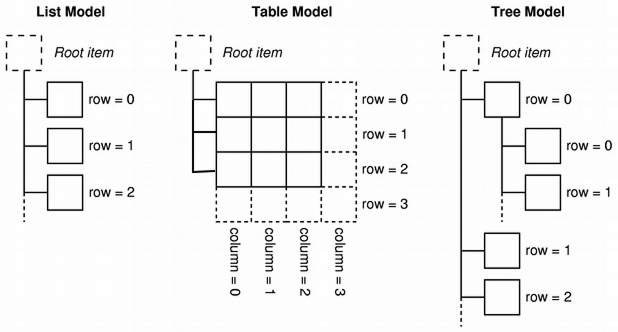
\includegraphics[width=0.5\textwidth]{list_table_tree}
\end{figure}

到目前为止,我们在示例中使用的模型都是这样子的:

\begin{figure}[hbt!]  
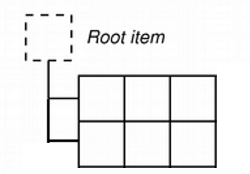
\includegraphics[width=0.5\textwidth]{example_model}
\end{figure}

我们想呈现一棵真正的树。在上面的示例中包装了数据,以建立模型。这次我们使用 QStandardItemModel ,这是用于具有层次结构的数据的容器,也实现了 QAbstractItemModel。
要显示树,必须用 QStandardItem 填充 QStandardItemModelQStandardItem 可以保存项目的所有标准属性,例如文本,字体,复选框或笔刷。

\begin{figure}[hbt!]  
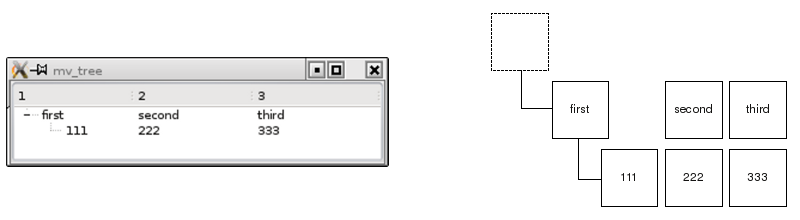
\includegraphics[width=0.5\textwidth]{tree_2_with_algorithm}
\end{figure}

(文件:\hl{examples/widgets/tutorials/modelview/6\_treeview/mainwindow.cpp})

\begin{cppcode}
// modelview.cpp
#include "mainwindow.h"

#include <QTreeView>
#include <QStandardItemModel>
#include <QStandardItem>

MainWindow::MainWindow(QWidget *parent)
    : QMainWindow(parent)
    , treeView(new QTreeView(this))
    , standardModel(new QStandardItemModel(this))
{
    setCentralWidget(treeView);

    QList<QStandardItem *> preparedRow = prepareRow("first", "second", "third");
    QStandardItem *item = standardModel->invisibleRootItem();
    // adding a row to the invisible root item produces a root element
    item->appendRow(preparedRow);

    QList<QStandardItem *> secondRow = prepareRow("111", "222", "333");
    // adding a row to an item starts a subtree
    preparedRow.first()->appendRow(secondRow);

    treeView->setModel(standardModel);
    treeView->expandAll();
}

QList<QStandardItem *> MainWindow::prepareRow(const QString &first,
                                              const QString &second,
                                              const QString &third) const
{
    return {new QStandardItem(first),
            new QStandardItem(second),
            new QStandardItem(third)};
}
\end{cppcode}

我们只需实例化一个 QStandardItemModel 并向构造函数添加几个 QStandardItem。
然后,我们可以建立分层数据结构,因为 QStandardItem 可以容纳其他 QStandardItem。节点在视图内折叠并展开。

\subsection{处理选择}

我们希望访问所选项目的内容,以便将其与层次结构级别一起输出到窗口标题中。

\begin{figure}[hbt!]  
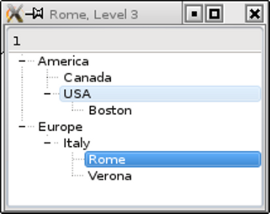
\includegraphics[width=0.5\textwidth]{selection2}
\end{figure}

因此,让我们来创建几个项:

(文件: \hl{examples/widgets/tutorials/modelview/7\_selections/mainwindow.cpp})

\begin{cppcode}
#include "mainwindow.h"

#include <QTreeView>
#include <QStandardItemModel>
#include <QItemSelectionModel>

MainWindow::MainWindow(QWidget *parent)
    : QMainWindow(parent)
    , treeView(new QTreeView(this))
    , standardModel(new QStandardItemModel(this))
{
    setCentralWidget(treeView);
    QStandardItem *rootNode = standardModel->invisibleRootItem();

    //defining a couple of items
    QStandardItem *americaItem = new QStandardItem("America");
    QStandardItem *mexicoItem =  new QStandardItem("Canada");
    QStandardItem *usaItem =     new QStandardItem("USA");
    QStandardItem *bostonItem =  new QStandardItem("Boston");
    QStandardItem *europeItem =  new QStandardItem("Europe");
    QStandardItem *italyItem =   new QStandardItem("Italy");
    QStandardItem *romeItem =    new QStandardItem("Rome");
    QStandardItem *veronaItem =  new QStandardItem("Verona");

    //building up the hierarchy
    rootNode->    appendRow(americaItem);
    rootNode->    appendRow(europeItem);
    americaItem-> appendRow(mexicoItem);
    americaItem-> appendRow(usaItem);
    usaItem->     appendRow(bostonItem);
    europeItem->  appendRow(italyItem);
    italyItem->   appendRow(romeItem);
    italyItem->   appendRow(veronaItem);

    //register the model
    treeView->setModel(standardModel);
    treeView->expandAll();

    //selection changes shall trigger a slot
    QItemSelectionModel *selectionModel = treeView->selectionModel();
    connect(selectionModel, &QItemSelectionModel::selectionChanged,
            this, &MainWindow::selectionChangedSlot);
}
\end{cppcode}

视图在单独的选择模型中管理选择,可以使用 selectionModel() 方法进行检索。我们检索选择模型,以便将槽函数连接到其 selectionChanged() 信号。

(文件: \hl{examples/widgets/tutorials/modelview/7\_selections/mainwindow.cpp})

\begin{cppcode}
void MainWindow::selectionChangedSlot(const QItemSelection & /*newSelection*/, const QItemSelection & /*oldSelection*/)
{
    //get the text of the selected item
    const QModelIndex index = treeView->selectionModel()->currentIndex();
    QString selectedText = index.data(Qt::DisplayRole).toString();
    //find out the hierarchy level of the selected item
    int hierarchyLevel = 1;
    QModelIndex seekRoot = index;
    while (seekRoot.parent() != QModelIndex()) {
        seekRoot = seekRoot.parent();
        hierarchyLevel++;
    }
    QString showString = QString("%1, Level %2").arg(selectedText)
                         .arg(hierarchyLevel);
    setWindowTitle(showString);
}
\end{cppcode}

我们通过调用 treeView->selectionModel()->currentIndex() 来获得与选择相对应的模型索引,并通过使用模型索引来获取字段的字符串。
然后我们只计算项目的hierarchyLevel。顶级项没有父级,并且 parent() 方法将返回默认构造的 QModelIndex()。这就是为什么我们在迭代计算期间使用 parent() 方法迭代到最高级别的原因。

可以检索选择模型(如上所示),但也可以使用 QAbstractItemView::setSelectionModel 进行设置。
这样就可以拥有3个具有同步选择的视图类,因为仅使用了一个选择模型实例。要在3个视图之间共享选择模型,请使用 selectionModel() 并通过 setSelectionModel 将结果分配给第二个和第三个视图类。

\subsection{预定义模型}

使用模型/视图的典型方法是包装特定数据以使其可用于视图类。
但是,Qt 还为常见的底层数据结构提供了预定义的模型。
如果可用的数据结构之一适合您的应用程序,那么预定义的模型可能是一个不错的选择。

\begin{longtable}[l]{|l|l|}
\hline
QStringListModel &	存储字符串列表 \\ 
\hline
QStandardItemModel &	存储任意分层结构的项目\\
\hline
QFileSystemModel
QDirModel	 & 封装本地文件系统\\ 
\hline
QSqlQueryModel &	封装 SQL 结果集\\
\hline
QSqlTableModel	& 封装 SQL 表\\
\hline
QSqlRelationalTableModel &	封装带外键的 SQL 表 \\
\hline
QSortFilterProxyModel	& 排序或者过滤其他模型 \\
\hline
\end{longtable}

\subsection{委托}

到目前为止,在所有示例中,数据均以文本或复选框形式显示在单元格中,并以文本或复选框的形式进行编辑。
提供这些表示和编辑服务的组件称为委托。我们只是刚刚开始使用委托,因为视图使用了默认委托。
但是,假设我们想要一个不同的编辑器(例如,一个滑块或一个下拉列表),或者想象我们想要将数据显示为图形。
让我们看一个名为 Star Delegate 的示例,其中的星星用于显示等级:


\begin{figure}[hbt!]  
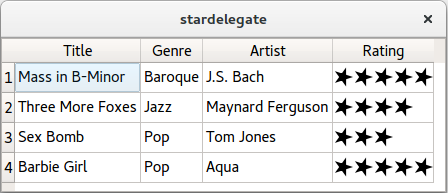
\includegraphics[width=0.5\textwidth]{stardelegate}
\end{figure}

该视图具有 setItemDelegate() 方法,该方法将替换默认委托并安装自定义委托。
可以通过创建从 QStyledItemDelegate 继承的类来编写新的委托。为了编写一个显示星星但没有输入功能的委托,我们只需要重写2个方法即可。


\begin{cppcode}
class StarDelegate : public QStyledItemDelegate
{
    Q_OBJECT
public:
    StarDelegate(QWidget *parent = 0);
    void paint(QPainter *painter, const QStyleOptionViewItem &option,
               const QModelIndex &index) const;
    QSize sizeHint(const QStyleOptionViewItem &option,
                   const QModelIndex &index) const;
};
\end{cppcode}

paint() 根据底层数据的内容绘制星形。可以通过调用 index.data() 查找数据。委托的 sizeHint() 方法用于获取每个星星的尺寸,因此该单元格将提供足够的高度和宽度来容纳星星。

如果要在视图类的网格内以自定义图形显示数据,则编写自定义委托是正确的选择。如果要离开网格,则可以不使用自定义委托,而使用自定义视图类。

Qt 文档中关于委托的其他参考:

\begin{compactitem}
\item Spin Box Delegate Example
\item QAbstractItemDelegate Class Reference
\item QSqlRelationalDelegate Class Reference
\item QStyledItemDelegate Class Reference
\item QItemDelegate Class Reference
\end{compactitem}

\subsection{使用 ModelTest 调试}

模型的被动性质为程序员带来了新的挑战。模型中的不一致会导致应用程序崩溃。
由于该模型会被视图中调用无数次,因此很难找出哪个调用使应用程序崩溃了,以及哪个操作导致了该问题。

Qt Labs 提供了一个名为 ModelTest 的软件,该软件可在您的程序运行时检查模型。
每次更改模型时,ModelTest 都会扫描模型并使用断言报告错误。这对于树模型尤其重要,因为它们的层次结构性质即使是细微的不一致也会留下许多可能性。

与视图类不同,ModelTest 使用超出范围的索引来测试模型。
这意味着您的应用程序可能会因 ModelTest 而崩溃,即使没有它也可以完美运行。因此,在使用 ModelTest 时,您还需要处理所有超出范围的索引。

\section{附录}
\subsection{书籍}

模型/视图编程在 Qt 文档中有相当广泛的介绍,但也有好几本好书。

\begin{compactitem}
\item C++ GUI Programming with Qt 4 / Jasmin Blanchette, Mark Summerfield, Prentice Hall, 2nd edition, ISBN 0-13-235416-0. 
      Also available in German: C++ GUI Programmierung mit Qt 4: Die offizielle Einführung, Addison-Wesley, ISBN 3-827327-29-6
\item The Book of Qt4, The Art of Building Qt Applications / Daniel Molkentin, Open Source Press, ISBN 1-59327-147-6. 
      Translated from Qt 4, Einführung in die Applikationsentwicklung, Open Source Press, ISBN 3-937514-12-0.
\item Foundations of Qt Development / Johan Thelin, Apress, ISBN 1-59059-831-8.
\item Advanced Qt Programming / Mark Summerfield, Prentice Hall, ISBN 0-321-63590-6. 
      This book covers Model/View programming on more than 150 pages.
\end{compactitem}

以下列表概述了上面列出的前三本书中包含的示例程序。
其中一些为开发类似应用程序提供了非常好的模板。

\begin{longtable}[l]{|m{15em}|l|l|l|m{15em}|}
\hline
示例名称 &	使用的视图类	&使用的模型&	涵盖的方面  \\ 
\hline	
Team Leaders &	QListview	&QStringListModel	&	&Book 1, Chapter 10, Figure 10.6 \\
\hline	
Directory Viewer	&QTreeView	&QDirModel	&	&Book 1, Chapter 10, Figure 10.7\\
\hline	
Color Names	 & QListView &	应用于 QStringListModel 的 QSortFilterProxyModel &&		Book 1, Chapter 10, Figure 10.8 \\
\hline	
Currencies &	QTableView &	基于 QAbstractTableModel 的自定义模型 &	只读 	&Book 1, Chapter 10, Figure 10.10  \\ 
\hline
Cities  &	QTableView &	基于 QAbstractTableModel 的自定义模型 &	读/写	&Book 1, Chapter 10, Figure 10.12 \\ 
\hline
Boolean Parser &	QTreeView	& 基于 QAbstractTableModel 的自定义模型	 & 只读 	&Book 1, Chapter 10, Figure 10.14 \\ 
\hline
Track Editor &	QTableWidget &	& 	自定义的委托并提供了自定义的编辑器  &	Book 1, Chapter 10, Figure 10.15 \\ 
\hline
Four directory views &	QListView QTableView QTreeView &	QDirModel	& 演示使用多个视图	&Book2, Chapter 8.2 \\ 
\hline
Address Book &	QListView QTableView QTreeView	& 基于 QAbstractTableModel 的自定义模型& 	读/写 &	Book2, Chapter 8.4 \\
\hline
Address Book with sorting  &		& QSortfilterProxyModel &	引入排序和过滤功能 &	Book2, Chapter 8.5 \\ 
\hline
Address Book with checkboxes &	& &		在模型/视图中引入复选框	 &Book2, Chapter 8.6 \\ 
\hline
Address Book with transposed grid	&	基于 QAbstractProxyModel 的自定义代理模型	& 引入自定义模型 &	Book2, Chapter 8.7 \\ 
\hline
Address Book with drag and drop		& &	引入托拖放支持	& Book2, Chapter 8.8 \\ 
\hline
Address Book with custom editor	&	&	引入自定义委托	& Book2, Chapter 8.9 \\
\hline
Views	& QListView QTableView QTreeView &	QStandardItemModel	& 只读	& Book 3, Chapter 5, figure 5-3 \\ 
\hline
Bardelegate	& QTableView	& &	演示基于 QAbstractItemDelegate 的自定义委托	& Book 3, Chapter 5, figure 5-5 \\ 
\hline
Editdelegate &	QTableView	& &		基于 QAbstractItemDelegate 的用于编辑的自定义委托	&Book 3, Chapter 5, figure 5-6 \\ 
\hline
Singleitemview	& 基于 QAbstractItemView 的自定义视图	&&	自定义视图	&Book 3, Chapter 5, figure 5-7 \\ 
\hline
listmodel &	QTableView	&基于 QAbstractTableModel 的自定义模型	&只读&	Book 3, Chapter 5, Figure 5-8 \\ 
\hline
treemodel	& QTreeView	& 基于 QAbstractTableModel 的自定义模型	&只读	&Book 3, Chapter 5, Figure 5-10 \\ 
\hline
edit integers &	[QListView]	& 基于 QAbstractTableModel 的自定义模型	 & 读/写	& Book 3, Chapter 5, Listing 5-37, Figure 5-11 \\ 
\hline
sorting	 & QTableView	& 应用于 QStringListModel 的 QSortFilterProxyModel	& 演示排序	& Book 3, Chapter 5, Figure 5-12 \\ 
\hline
\end{longtable}

\subsection{Qt 文档}

Qt5.0提供了19个模型/视图示例。这些示例可以在 项目视图示例 页面上找到。


\begin{longtable}[l]{|l|m{10em}|m{10em}|l|}
\hline
示例名称	& 使用的视图类	& 使用的模型 & 	涵盖的方面  \\ 
\hline
Address Book &	QTableView &QAbstractTableModel QSortFilterProxyModel &	使用QSortFilterProxyModel从一个数据池生成不同的子集 \\ 
\hline
Basic Sort/Filter Model	& QTreeView &	QStandardItemModel QSortFilterProxyModel & 	 \\ 
\hline
Chart	& 自定义视图	& QStandardItemModel	& 设计与选择模型协作的自定义视图 \\ 
\hline
Color Editor Factory &	QTableWidget	&&	扩展一个带有新的自定义的编辑器的委托来选择颜色 \\ 
\hline
Combo Widget Mapper &使用 [QDataWidgetMapper] () 映射 QLineEdit、QTextEdit 和 QComboBox	 & QStandardItemModel	& 演示了QComboBox如何作为视图类 \\ 
\hline
Custom Sort/Filter Model &	QTreeView &	QStandardItemModel QSortFilterProxyModel &	子类化 QSortFilterProxyModel 用于高级排序和过滤 \\ 
\hline
Dir View &	QTreeView &	QFileSystemModel &	演示如何将模型指定给视图的非常小的示例 \\ 
\hline
Editable Tree Model	 &QTreeView	 &自定义树模型	& 使用树的综合示例,演示了如何使用底层自定义模型编辑单元格和树结构 \\ 
\hline
Fetch More&	QListView	&自定义列表模型 &	动态变化的模型 \\ 
\hline
Frozen Column &	QTableView	& QStandardItemModel	& \\ 
\hline
Interview &	Multiple	 & 自定义项目模型 &	多个视图 \\ 
\hline
Pixelator	& QTableView	& 自定义表模型	& 实现一个自定义委托 \\ 
\hline
Puzzle	& QListView	& 自定义列表模型 &	支持拖放的模型/视图 \\ 
\hline
Simple DOM Model&	QTreeView	 & 自定义树模型 &	自定义的只读的树模型的示例 \\ 
\hline
Simple Tree Model	 & QTreeView	& 自定义树模型	& 自定义的只读的树模型的示例 \\ 
\hline
Simple Widget Mapper&	使用 QDataWidgetMapper 映射 QLineEdit、QTextEdit 和 QSpinBox&	QStandardItemModel &	QDataWidgetMapper 的基本用法 \\ 
\hline
Spin Box Delegate & 	QTableView &	QStandardItemModel &	使用旋转框作为单元格编辑器的自定义委托 \\ 
\hline 
Spreadsheet	& QTableView	 &&	自定义委托  \\ 
\hline 
Star Delegate &	QTableWidget	&&	功能齐全的自定义委托示例 \\ 
\hline
\end{longtable}

还提供了模型/视图技术的参考文档。
\chapter{Qt 中的多线程技术}

Qt 提供一系列的类与函数来处理多线程。Qt 开发者们可以使用下面四种方法来实现多线程应用。

\section{QThread: 低级 API 与可选的事件循环}

作为 Qt 进行线程控制的基石,每一个 QThread 实例都代表并控制着一个线程。

您可以直接实例化 QThread,或建立子类。实例化一个 QThread 将附带一个并行事件循环,
允许 QObject 槽函数在子线程执行。若子类化一个 QThread,程序可以在事件循环启动前初始化这个新线程;
或者在无事件循环下运行并行代码。

\begin{notice}[另请参阅]
QThread 类文档 以及示例代码 多线程范例 来了解如何使用 QThread。
\end{notice}

\section{QThreadPool 与 QRunnable: 线程重用}

如果频繁地创建与销毁线程,资源开销将会非常大。为了减少这样额外的开销,可以重复使用一些现成的线程来执行新的任务。QThreadPool 就是这样一个保存着可重用的 QThead 的集合。

为了将代码放入 QThreadPool 的线程中运行,可以重写 QRunnable::run() 函数并实例化继承自 QRunnable 的子类。调用 QThreadPool::start() 函数可将 QRunnable 添加到 QThreadPool 的运行队列。一旦出现了一个可用的线程,它将会执行 QRunnable::run() 里的代码。

每一个 Qt 程序都会自带一个公共线程池,可以通过调用 QThreadPool::globalInstance() 来获取。公共线程池会自动维持着一定数量的线程,线程数为基于 CPU 核心数计算的最佳值。不过,您也可以显式创建并管理一个独立的 QThreadPool 。

\begin{notice}[另请参阅]
Qt Concurrent 模块文档以获取各个函数的详细信息。
\end{notice}
    


\section{Qt Concurrent: 使用高级 API}

Qt Concurrent 模块提供了数个高级函数,用于处理一些常见的并行计算模式:map、filter 和 reduce。
不同于使用 QThread 与 QRunnable,这些高级函数不需要使用底层线程原语,比如互斥锁与信号量。
取而代之的是返回一个 QFuture 对象,它能够在传入的函数返回值就绪后检索该结果。
QFuture 既可以用来查询计算进度,也可以暂停/恢复/取消计算。
方便起见,QFutureWatcher 可以让您通过信号槽与 QFuture 进行交互。

Qt Concurrent 的 map、filter 和 reduce 算法会自动将计算过程分配到可用的处理器核心,
由此,当下编写的程序在以后部署到更多核心的系统上时会被自动扩展。

此模块还提供了 QtConcurrent::run() 函数,可以将任何函数在另一个线程中运行。
不过,QtConcurrent::run() 仅提供 map 、 filter 和 reduce 函数的一部分功能。
QFuture 可以用于检索函数返回值,也可以用于查看线程是否处于运行中。
然而,调用 QtConcurrent::run() 时只会使用一个线程,并且无法暂停/恢复/取消,也不能查询计算进度。



\section{WorkerScript: QML中的多线程}

QML 类型 WorkerScript 可将 JavaScript 代码与 GUI 线程并行运行。

每个 WorkerScript 实例可附加一个 .js 脚本。当调用 WorkerScript.sendMessage() 时,
脚本将会运行在一个独立的线程中(伴随一个独立的 QML 上下文)。
在脚本运行结束后,WorkerScript 将会向 GUI 线程发送回复,
后者会调用 WorkerScript.onMessage() 信号处理函数。

使用 WorkerScript,很像使用一个移入子线程工作的 QObject,数据通过信号槽在线程间进行传输。

\begin{notice}[另请参阅]
WorkerScript 文档以获得实现脚本的详细信息,以及能够在线程间传输的数据类型列表。
\end{notice}

\section{选择合适的方法}

如上文所述,Qt 提供了开发多线程应用的不同解决方案。
对一个给定的程序,需要根据新线程的用途与线程的生命周期来决定正确的方案。
下面是一组 Qt 多线程技术的功能对比表,以及对于一些范例较为推荐的解决方案。


\section{解决方案对比}

\begin{longtable}{|l|l|l|l|l|l|}
\hline
特性  &	QThread &	QRunnable 与 QThreadPool 	& QtConcurrent::run() &	Qt Concurrent(Map, Filter, Reduce) & 	WorkerScript \\ 
\hline
语言 &	C++ &	C++ &	C++ &	C++ &	QML \\ 
\hline
可以指定线程优先级 & 	是 & 	是   & & & \\ 
\hline
可以在线程中运行运行事件循环 	&是 &&&& 		 \\ 
\hline
可以通过信号获取数据更新 	&是(通过 QObject 对象接收) & & & &				是(通过 WorkerScript 接收) \\ 
\hline
可以使用信号控制线程 	& 是(通过 QThread 接收) & & 			是(通过 QFutureWatcher 接收) &&	 \\ 
\hline
可以通过QFuture 监视线程 	&&		部分适用(译者注:仅可监视返回值,不可监视执行进度) 	&是 && 	 \\ 
\hline
内建的暂停/恢复/取消功能 		& & &		是 & &	 \\ 
\hline
\end{longtable}

\section{示例用例}


\begin{longtable}{|l|m{10em}|m{15em}|}
\hline
线程生命周期 	& 操作 	 & 解决方案   \\ 
\hline
单次调用 	& 在另一个线程中运行新的线性函数,可选地在运行期间进行更新进度。 &	Qt 提供不同解决方案:
1. 重写 QThread::run() 并将函数放入其中,启动 QThread ,发射信号来更新进度。
2. 重写 QRunnable::run() ,将函数放入其中。将 QRunnable 添加到 QThreadPool 中。修改线程安全的变量以更新进度;
3. 使用 QtConcurrent::run() 运行函数。修改线程安全变量以更新进度。\\ 
\hline
单次调用 &	在另一个线程中运行一个现成的函数,并取得它的返回值。 	& 使用 QtConcurrent::run() 运行函数。让 QFutureWatcher 在函数返回时发射 finish() 信号,并调用 QFutureWatcher::result() 来获取函数的返回值。 \\ 
\hline
单次调用 &	对一个容器的所有元素执行一个操作,使用所有可用的 CPU 核心。例如,从一组图片生成缩略图。 &	使用 Qt Concurrent 的 QtConcurrent::filter() 函数选择容器元素,并用 QtConcurrent::map() 函数对每个元素执行操作。要将输出合并为单个结果,可以使用 QtConcurrent:: filteredReduced() 和 QtConcurrent::mappedReduced()。 \\ 
\hline
单次调用/长期存在 &	在纯 QML 应用中执行耗时计算,并在结果就绪时更新 GUI 。 &	将计算代码放在 .js 脚本中,将它附加在 WorkerScript 实例上。调用 WorkerScript.sendMessage() 启动新线程执行计算。脚本也同样调用 sendMessage(),将结果传回 GUI 线程。在 onMessage 中处理结果并且更新 GUI 。 \\ 
\hline
长期存在 & 对象位于另一个线程中,可以根据请求执行不同的任务和/或接收要使用的新数据。 &	子类化一个 QObject 以创建一个工作类。实例化这个工作类对象与一个 QThread 。将工作类移入新线程。通过队列信号槽的连接,将命令与数据传递给工作类对象。 \\ 
\hline
长期存在 &	在另一个不需要接收任何信号或事件的线程中,重复执行资源开销大的操作。 & 	直接重写 QThread::run() 并创建死循环。启动无事件循环的线程。可以发送信号将数据送回 GUI 线程(译者注:发送信号不需要依赖事件循环,接收并执行槽函数才需要)。 \\
\hline
\end{longtable}
\chapter{QMainWindow}

QMainWindow 类用于创建主程序窗口。 更多内容...


\begin{tabular}{|r|l|}
	\hline
	属性 & 方法 \\
	\hline
	头文件 & \#include <QMainWindow>\\      
	\hline
	qmake & QT += widgets\\      
	\hline
	继承: &	QWidget\\
	\hline
\end{tabular}

\begin{compactitem}
\item 列出所有成员函数, 包括继承的成员函数
\end{compactitem}

\section{公共成员类型}

\begin{tabular}{|r|m{25em}|}
	\hline
	类型 & 方法 \\
	\hline
    enum &	DockOption \{ AnimatedDocks, AllowNestedDocks, AllowTabbedDocks, ForceTabbedDocks, VerticalTabs, GroupedDragging \} \\ 
    \hline
    flags &	DockOptions \\ 
	\hline
\end{tabular}

\section{属性}

\begin{tabular}{|r|l|}
	\hline
    属性名 &	类型 \\ 
    \hline
    animated 	& bool \\ 
    \hline
    dockNestingEnabled &	bool\\
    \hline
    dockOptions &	DockOptions\\
    \hline
    documentMode 	&bool\\
    \hline
    iconSize  &	QSize\\
    \hline
    tabShape 	&QTabWidget::TabShape\\
    \hline
    toolButtonStyle &	Qt::ToolButtonStyle\\
    \hline
    unifiedTitleAndToolBarOnMac &	bool\\
	\hline
\end{tabular}

\section{公共成员函数}

\begin{longtable}{|r|m{20em}|}
\hline
返回类型  & 	函数名 \\
\hline
 &QMainWindow (QWidget *parent = nullptr, Qt::WindowFlags flags = Qt::WindowFlags()) \\ 
 \hline
virtual  &	$\sim$QMainWindow () \\
\hline
void 	&addDockWidget (Qt::DockWidgetArea area, QDockWidget *dockwidget) \\ 
\hline
void 	&addDockWidget (Qt::DockWidgetArea area, QDockWidget *dockwidget, Qt::Orientation orientation) \\
\hline
void 	&addToolBar (Qt::ToolBarArea area, QToolBar *toolbar) \\ 
\hline
void 	&addToolBar (QToolBar *toolbar) \\ 
\hline
QToolBar *& 	addToolBar (const QString \&title) \\
\hline
void 	&addToolBarBreak (Qt::ToolBarArea area = Qt::TopToolBarArea) \\
\hline
QWidget *& 	centralWidget () const \\ 
\hline
Qt::DockWidgetArea &	corner (Qt::Corner corner) const \\
\hline
virtual QMenu * &	createPopupMenu () \\
\hline
QMainWindow::DockOptions& 	dockOptions () const\\
\hline
Qt::DockWidgetArea 	&dockWidgetArea (QDockWidget *dockwidget) const\\
\hline
bool &	documentMode () const \\
\hline
QSize &	iconSize () const\\
\hline
void 	&insertToolBar (QToolBar *before, QToolBar *toolbar)\\
\hline
void 	&insertToolBarBreak (QToolBar *before)\\
\hline
bool 	&isAnimated () const\\
\hline
bool 	&isDockNestingEnabled () const\\
\hline
QMenuBar *& 	menuBar () const \\ 
\hline
QWidget * &	menuWidget () const \\ 
\hline
void 	&removeDockWidget (QDockWidget *dockwidget)\\ 
\hline
void 	&removeToolBar (QToolBar *toolbar) \\ 
\hline
void 	&removeToolBarBreak (QToolBar *before) \\ 
\hline
void 	&resizeDocks (const QList<QDockWidget *> \&docks, const QList<int> \&sizes, Qt::Orientation orientation) \\ 
\hline
bool 	&restoreDockWidget (QDockWidget *dockwidget) \\ 
\hline
bool 	&restoreState (const QByteArray \&state, int version = 0) \\ 
\hline
QByteArray &	saveState (int version = 0) const \\ 
\hline
void &	setCentralWidget (QWidget *widget) \\ 
\hline
void &	setCorner (Qt::Corner corner, Qt::DockWidgetArea area) \\ 
\hline
void 	&setDockOptions (QMainWindow::DockOptions options) \\ 
\hline
void &	setDocumentMode (bool enabled) \\ 
\hline
void &	setIconSize (const QSize \&iconSize) \\ 
\hline
void &	setMenuBar (QMenuBar *menuBar) \\ 
\hline
void& 	setMenuWidget (QWidget *menuBar) \\ 
\hline
void &	setStatusBar (QStatusBar *statusbar) \\ 
\hline
void &	setTabPosition (Qt::DockWidgetAreas areas, QTabWidget::TabPosition tabPosition) \\ 
\hline
void &	setTabShape (QTabWidget::TabShape tabShape) \\ 
\hline
void 	&setToolButtonStyle (Qt::ToolButtonStyle toolButtonStyle) \\ 
\hline
void 	&splitDockWidget (QDockWidget *first, QDockWidget *second, Qt::Orientation orientation) \\ 
\hline
QStatusBar * & 	statusBar () const \\ 
\hline
QTabWidget::TabPosition &	tabPosition (Qt::DockWidgetArea area) const \\ 
\hline
QTabWidget::TabShape & 	tabShape () const \\
\hline
QList<QDockWidget *> 	&tabifiedDockWidgets (QDockWidget *dockwidget) const \\
\hline
void &	tabifyDockWidget (QDockWidget *first, QDockWidget *second) \\ 
\hline
QWidget *& 	takeCentralWidget () \\ 
\hline
Qt::ToolBarArea &	toolBarArea (QToolBar *toolbar) const \\ 
\hline
bool &	toolBarBreak (QToolBar *toolbar) const \\ 
\hline
Qt::ToolButtonStyle & 	toolButtonStyle () const \\ 
\hline
bool &	unifiedTitleAndToolBarOnMac () const \\
\hline
\end{longtable}

\section{公共槽}

\begin{tabular}{|r|l|}
\hline
返回类型 &	函数名 \\
\hline
void 	&setAnimated (bool enabled) \\ 
\hline
void 	&setDockNestingEnabled (bool enabled) \\
\hline
void 	&setUnifiedTitleAndToolBarOnMac (bool set) \\
\hline
\end{tabular}

\section{信号}

\begin{tabular}{|r|l|}
    \hline
    返回类型 &	函数名 \\
    \hline
    void &	iconSizeChanged (const QSize \&iconSize) \\ 
    \hline
    void &	tabifiedDockWidgetActivated (QDockWidget *dockWidget) \\ 
    \hline
    void &	toolButtonStyleChanged (Qt::ToolButtonStyle toolButtonStyle) \\
    \hline
\end{tabular}

\section{保护成员函数}

\begin{tabular}{|r|l|}
\hline
返回类型 &	函数名 \\
\hline
virtual void &	contextMenuEvent (QContextMenuEvent *event) override \\
\hline
virtual bool &	event (QEvent *event) override \\
\hline
\end{tabular}

\section{详细描述}
\subsection{Qt 主窗口框架}

主窗口提供了一套创建应用程序用户界面的框架。 Qt 用QMainWindow和 相关类 来管理主窗口。QMainWindow已经定义了一个布局,可以往里添加一些 QToolBar 和 QDockWidget,也可以添加一个 QMenuBar 和一个 QStatusBar。这个布局有一个中央区域,可以放任意部件。如下图所示:

main window layout

\begin{notice}
主窗口必须设置中央部件。
\end{notice}

\subsection{创建主窗口组件}

中央部件通常是标准 Qt 部件,如 QTextEdit 或 QGraphicsView,也可自定义部件。
用setCentralWidget()来设置中央部件。

主窗口可以是单文档界面或多文档界面。 
Qt 中设置 QMdiArea 为中央部件即创建了多文档界面。

下面举例说明主窗口可以添加的部件。

\subsubsection{创建菜单}

Qt 用 QMenu 类实现菜单,主窗口将其放在 QMenuBar。
可以添加 QAction 到QMenu,一个QAction代表菜单中的一个条目。

用menuBar()可以得到主窗口的菜单栏,用 QMenuBar::addMenu 添加菜单。

QMainWindow 默认有一个菜单栏,可以用setMenuBar()自定义一个新的菜单栏。
如果不想用 QMenuBar ,也可以用setMenuWidget()来定制菜单栏。

创建菜单代码示例:

\begin{lstlisting}{language=C++}
void MainWindow::createMenus()
{
    fileMenu = menuBar()->addMenu(tr("&File"));
    fileMenu->addAction(newAct);
    fileMenu->addAction(openAct);
    fileMenu->addAction(saveAct);
}
\end{lstlisting}

createPopupMenu()可以创建弹出式菜单,它会在主窗口收到 context menu 事件时弹出。
停靠部件和菜单栏默认实现了右键菜单,可以重写createPopupMenu()创建自定义菜单。

\subsubsection{创建工具栏}

Qt 用 QToolBar 类实现工具栏,可以用addToolBar()添加工具栏到主窗口。

可以设置 Qt::ToolBarArea 来控制工具栏的初始位置。可以用addToolBarBreak()或insertToolBarBreak()分割工具栏所在的区域,前者可使接下来添加的工具栏换至新的一行,后者添加了一个工具栏分隔符。用 QToolBar::setAllowedAreas 加 QToolBar::setMovable 可以限制用户放工具栏的位置。

工具栏图标的尺寸可以用iconSize()获取,它是平台相关的。可以用setIconSize()设置固定尺寸。用setToolButtonStyle()可以修改工具栏图标外观。

创建工具栏代码示例:

\begin{lstlisting}{language=C++}
void MainWindow::createToolBars()
{
    fileToolBar = addToolBar(tr("File"));
    fileToolBar->addAction(newAct);
}
\end{lstlisting}

\subsection{创建停靠部件}

Qt 用 QDockWidget 类实现停靠部件。停靠部件即可以停靠在主窗口的窗口,可以用 \hl{addDockWidget()} 添加停靠部件到主窗口。

可以设置 \hl{Qt::DockWidgetArea} 来控制停靠部件的位置,有上、下、左、右四种。\hl{setCorner()} 可以让一个角落属于某个相邻的区域。
默认情况下,一个区域只有一个停靠部件,用 \hl{setDockNestingEnabled()} 可以使其能上下或者左右排列多个停靠部件。

两个停靠部件也可以堆叠在一起,然后使用 QTabBar 来选择应显示哪个部件。

创建并添加停靠部件到主窗口的代码示例:


\begin{lstlisting}[language=C++]
QDockWidget *dockWidget = new QDockWidget(tr("Dock Widget"), this);
dockWidget->setAllowedAreas(Qt::LeftDockWidgetArea | Qt::RightDockWidgetArea);
dockWidget->setWidget(dockWidgetContents);
addDockWidget(Qt::LeftDockWidgetArea, dockWidget);
\end{lstlisting}

\subsection{状态栏}

用 \hl{setStatusBar()} 可以设置状态栏,调用 \hl{statusBar()} 会返回主窗口的状态栏。查看 QStatusBar 获取更多内容。

\subsection{存储状态}

QMainWindow 用 \hl{saveState()} 保存布局,用 \hl{restoreState()} 恢复布局。包括工具栏和停靠部件的位置和相对主窗口的尺寸。

\begin{notice}[另请参阅]
QMenuBar,QToolBar,QStatusBar, QDockWidget,Application Example,
Dock Widgets Example,MDI Example,SDI Example 和 Menus Example。
\end{notice}

\section{成员变量文档}

enum QMainWindow::DockOption flags QMainWindow::DockOptions

该枚举包含指定 QMainWindow 停靠行为的标志。

\begin{tabular}{|l|l|m{25em}|}
\hline
函数	& 值	&描述 \\ 
\hline
QMainWindow::AnimatedDocks&	0x01	&同 animated 属性 \\
\hline
QMainWindow::AllowNestedDocks	&0x02&	同 dockNestingEnabled 属性 \\ 
\hline
QMainWindow::AllowTabbedDocks	&0x04	&允许形成下方有 tabBar 的重合部件 \\ 
\hline
QMainWindow::ForceTabbedDocks	&0x08&	每个停靠区域都只包含一个选项卡式停靠部件。
换句话说,停靠区域里不能上下或左右排列停靠部件。如果设置了此选项,则 AllowNestedDocks 不起作用。 \\
\hline
QMainWindow::VerticalTabs	&0x10	&设置 tabBar 在竖直左方位置(默认在下方),包含了 AllowTabbedDocks。另请参阅 setTabPosition () \\ 
\hline
QMainWindow::GroupedDragging	&0x20	&拖动停靠部件的标题栏时,将拖动所有和它在一起的停靠部件。
包含了 AllowTabbedDocks 。在某些停靠部件有区域限制时会有问题。(该枚举值在 Qt 5.6 添加) \\ 
\hline
\end{tabular}

这些选项只是控制停靠部件将如何放入 QMainWindow,不会重新排列停靠部件。
所以要先给停靠部件设置这些选项,再添加到主窗口。AnimatedDocks 和 VerticalTabs 选项例外,它们可以随后设置。

此枚举值在 Qt 4.3 引入和修改

DockOptions 是 QFlags<DockOption> 的 typedef。
它存储 DockOption 值的 OR 组合。

\section{属性文档}

animated : bool

此属性表示是否对操作停靠部件和工具栏进行动画处理

当停靠部件或工具栏在主窗口拖动时,主窗口会显示它们将停靠在什么位置。设置此属性使 QMainWindow 在平滑动画中移动其内容。清除此属性会使它们啪地进入新位置。

默认情况,此属性是生效的。如果主窗口调整尺寸或重绘太慢,可能会无效。

设置此属性与使用 setDockOptions () 设置 AnimatedDocks 选项相同。

该属性在 Qt 4.2 引入

存取函数:

\begin{tabular}{|c|c|}
\hline
    返回类型 &	函数名 \\ 
\hline
bool	& isAnimated() const \\ 
\hline
void	& setAnimated(bool enabled) \\ 
\hline
\end{tabular}

\splitLine

dockNestingEnabled : bool

此属性表示停靠部件是否可以嵌套。

如果此属性为false,停靠区域只能是水平的或垂直的一行。
如果此属性为true,停靠区域所占的区域可以沿任意方向拆分以包含更多的停靠部件。

\begin{quote}
译者注:如果设为 true,两个 dock 可以上面一块,
下面一块,显示在一个区域里,如果设为 false,
则两个 dock 只能变成选项卡式占用一个区域。
\end{quote}

只有在包含大量停靠部件的应用程序中,才需要停靠嵌套。
它给用户更大的自由来组织主窗口。但是,当停靠部件拖过主窗口时,停靠嵌套会导致更加复杂和不太直观的行为。

设置此属性与使用 setDockOptions () 设置 AllowNestedDocks 选项相同。

该属性在 Qt 4.2 引入

存取函数:

\begin{tabular}{|c|c|}
    \hline
    返回类型 &	函数名 \\ 
    \hline
    bool	& isDockNestingEnabled() const \\ 
    \hline
    void	& setDockNestingEnabled(bool enabled) \\ 
    \hline
    \end{tabular}

\splitLine

dockOptions : DockOptions

此属性表示 QMainWindow 的停靠行为

默认值是 AnimatedDocks | AllowTabbedDocks

该属性在 Qt 4.3 引入

存取函数:

\begin{tabular}{|c|c|}
    \hline
    返回类型 &	函数名 \\ 
    \hline
    QMainWindow::DockOptions &	dockOptions() const \\ 
    \hline
    void	&setDockOptions(QMainWindow::DockOptions options) \\ 
    \hline
    \end{tabular}

\splitLine

documentMode : bool

此属性决定选项卡式停靠部件的选项卡栏是否为文档模式。

默认为 false

该属性在 Qt 4.5 引入

存取函数:

\begin{tabular}{|c|c|}
    \hline
    返回类型 &	函数名 \\ 
    \hline
    bool&	documentMode() const \\ 
    \hline
    void&	setDocumentMode(bool enabled) \\ 
    \hline
    \end{tabular}

\begin{notice}[另请参阅]
QTabBar::documentMode
\end{notice}

\splitLine

iconSize : QSize

主窗口工具栏图标的尺寸。

默认是 GUI 样式的默认工具栏图标大小。

\begin{notice}
使用的图标必须至少具有此大小,因为图标只会缩小。
\end{notice}

存取函数:

\begin{tabular}{|c|c|}
    \hline
    返回类型 &	函数名 \\ 
    \hline 
    QSize	&iconSize() const \\ 
    \hline
    void&	setIconSize(const QSize \&iconSize) \\
    \hline
    \end{tabular}

\splitLine

tabShape : QTabWidget::TabShape

此属性表示选项卡式停靠部件的选项卡形状。

默认是 QTabWidget::Rounded

该属性在 Qt 4.5 引入

存取函数:

\begin{tabular}{|c|c|}
    \hline
    返回类型 &	函数名 \\ 
    \hline  
    QTabWidget::TabShape &	tabShape() const \\ 
    \hline
    void 	& setTabShape(QTabWidget::TabShape tabShape) \\ 
    \hline
    \end{tabular}


\begin{notice}[另请参阅]
setTabPosition ()
\end{notice}

\splitLine

toolButtonStyle : Qt::ToolButtonStyle

主窗口的工具栏按钮样式。

若要使工具按钮的样式遵循系统设置,请将此属性设置为 Qt::ToolButtonFollowStyle。
在 Unix 上,将使用桌面环境变量中的用户设置。在其他平台上,Qt::ToolButtonFollowStyle 意思是仅显示图标。

默认是 Qt::ToolButtonIconOnly

存取函数:

\begin{tabular}{|c|c|}
    \hline
    返回类型 &	函数名 \\ 
    \hline  
    Qt::ToolButtonStyle &	toolButtonStyle() const \\ 
    \hline
    void 	& setToolButtonStyle(Qt::ToolButtonStyle toolButtonStyle) \\ 
    \hline
    \end{tabular}

\splitLine

unifiedTitleAndToolBarOnMac : bool

此属性表示窗口是否使用 macOS 上的统一标题和工具栏外观

请注意,与 Qt 4 相比,Qt 5 实现有几个限制:

\begin{compactitem}
\item 不支持在包含 OpenGL 内容的窗口中使用。这包括 QGLWidget 和 QOpenGLWidget。
\item 使用可停靠或可移动工具栏可能会导致绘制错误,不建议使用。
\end{compactitem}

该属性在 Qt 5.2 引入

存取函数:

\begin{tabular}{|c|c|}
    \hline
    返回类型 &	函数名 \\ 
    \hline  
    bool  &	unifiedTitleAndToolBarOnMac() const \\ 
    \hline
    void  &	setUnifiedTitleAndToolBarOnMac(bool set) \\ 
    \hline
    \end{tabular}

\section{成员函数文档}


QMainWindow::QMainWindow(QWidget *parent = nullptr, Qt::WindowFlags flags = Qt::WindowFlags())

主窗口构造函数,指定 parent 和 flags

主窗口设置了 Qt::Window 标志,因此它总作为顶层窗口被创建。

\splitLine

[signal]void QMainWindow::iconSizeChanged(const QSize \&iconSize)

当窗口图标被改变时,将发出此信号。新图标的尺寸为 iconSize。

您可以将此信号连接到其他组件,以帮助保持应用程序的一致外观。

\begin{notice}[另请参阅]
setIconSize ().
\end{notice}

\splitLine

[signal]void QMainWindow::tabifiedDockWidgetActivated(QDockWidget *dockWidget)

当通过选择选项卡激活停靠部件时,将发出此信号。 dockWidget 表示激活的停靠部件。

该函数在 Qt 5.8 引入

\begin{notice}[另请参阅]
tabifyDockWidget() and tabifiedDockWidgets()
\end{notice}

\splitLine

[signal]void QMainWindow::toolButtonStyleChanged(Qt::ToolButtonStyle toolButtonStyle)

当窗口的工具栏按钮样式更改时,将发出此信号。toolButtonStyle 表示新样式。

您可以将此信号连接到其他组件,以帮助保持应用程序的一致外观。

\begin{notice}[另请参阅]
setToolButtonStyle ()
\end{notice}

\splitLine

[virtual]QMainWindow::$\sim$QMainWindow()

销毁主窗口

\splitLine

void QMainWindow::addDockWidget(Qt::DockWidgetArea area, 
    QDockWidget *dockwidget)

添加指定 dockwidget 到指定 area.

\splitLine

void QMainWindow::addDockWidget(Qt::DockWidgetArea area, QDockWidget *dockwidget, Qt::Orientation orientation)

将 dockwidget 添加到指定的 area,方向由 orientation 指定。

\splitLine

void QMainWindow::addToolBar(Qt::ToolBarArea area, QToolBar *toolbar)

在主窗口中将 toolbar 添加到指定的 area。toolbar 放置在当前工具栏块(比如分隔符)的后面。如果主窗口已管理 toolbar,则只会将工具栏移动到 area。


\begin{notice}[另请参阅]
insertToolBar (),addToolBarBreak () 和 insertToolBarBreak ()
\end{notice}

\splitLine

void QMainWindow::addToolBar(QToolBar *toolbar)

这是一个重载函数。

相当于调用 addToolBar(Qt::TopToolBarArea, toolbar)

\splitLine

QToolBar *QMainWindow::addToolBar(const QString \&title)

这是一个重载函数。

创建 QToolBar 的一个对象,设置它的窗口标题为 title 并将它添加到上方的工具栏区域。

\begin{notice}[另请参阅]
setWindowTitle ()
\end{notice}

\splitLine

void QMainWindow::addToolBarBreak(Qt::ToolBarArea area = Qt::TopToolBarArea)

添加一个工具栏 break。这时,新添加的工具条将不再紧跟前一个工具条,而是另起一行。

\splitLine

QWidget *QMainWindow::centralWidget() const

返回主窗口的中央部件。如果尚未设置中央部件,则此函数返回零。

\begin{notice}[另请参阅]
setCentralWidget ()
\end{notice}

\splitLine

[override virtual protected]void QMainWindow::contextMenuEvent(QContextMenuEvent \emph{*event})

重写:QWidget::contextMenuEvent (QContextMenuEvent *event)

Qt::DockWidgetArea QMainWindow::corner(Qt::Corner corner) const

返回占用指定 corner 的停靠部件区域。

\begin{notice}[另请参阅]
setCorner ()
\end{notice}

\splitLine

[virtual]QMenu *QMainWindow::createPopupMenu()

返回一个弹出式菜单,其中包含主窗口中存在的工具栏和停靠部件的可选中条目。如果没有工具栏和停靠小部件,则此函数将返回nullptr。

默认情况下,当用户激活上下文菜单时,主窗口会调用此函数,通常通过右键单击工具栏或停靠部件。

如果要创建自定义弹出式菜单,请重新实现此功能并返回新创建的弹出式菜单。
弹出式菜单的所有权将传输到调用方。

\begin{notice}[另请参阅]
addDockWidget (),addToolBar () 和 menuBar ()
    \end{notice}
    
\splitLine

Qt::DockWidgetArea QMainWindow::dockWidgetArea(QDockWidget \emph{*dockwidget}) const

返回 dockwidget 的 Qt::DockWidgetArea。如果 dockwidget 没有被加入主窗口,此函数返回Qt::NoDockWidgetArea

\begin{notice}[另请参阅]
addDockWidget (),splitDockWidget () 和 Qt::DockWidgetArea
\end{notice}

\splitLine

[override virtual protected]bool QMainWindow::event(QEvent \emph{*event})

重写:QWidget::event (QEvent *event)

\splitLine

void QMainWindow::insertToolBar(QToolBar \emph{*before}, QToolBar \emph{*toolbar})

将 toolbar 插入到 before 工具栏占用的区域之前。
例如,在正常的从左到右布局操作中,toolbar 将显示在水平工具栏区域中 before 工具栏的左侧。

\begin{notice}[另请参阅]
insertToolBarBreak (),addToolBar () 和 addToolBarBreak ()
\end{notice}

\splitLine

void QMainWindow::insertToolBarBreak(QToolBar \emph{*before})

在 before 工具栏左侧插入一个工具栏 break。

\splitLine

QMenuBar *QMainWindow::menuBar() const

返回主窗口的菜单栏。如果菜单栏不存在,则此函数将创建并返回一个空菜单栏。

如果希望 Mac 应用程序中的所有窗口共享一个菜单栏,请不要使用此函数来创建它,
因为此处创建的菜单栏将把 QMainWindow 作为它的父对象。
必须创建一个没有父对象的菜单栏,然后可以在所有 Mac 窗口之间共享该菜单栏。

这样创建:

\begin{lstlisting}{language=C++}
QMenuBar *menuBar = new QMenuBar(nullptr);
\end{lstlisting}

\begin{notice}[另请参阅]
setMenuBar()
\end{notice}

\splitLine

QWidget *QMainWindow::menuWidget() const

返回主窗口的菜单栏。如果尚未构造菜单栏,返回 null。

该函数在 Qt 4.2 引入

\begin{notice}[另请参阅]
setMenuWidget ()
\end{notice}

\splitLine

void QMainWindow::removeDockWidget(QDockWidget \emph{*dockwidget})

从主窗口布局中移除 dockwidget 并将其隐藏。注意,dockwidget 没有被 delete。

\splitLine

void QMainWindow::removeToolBar(QToolBar \emph{*toolbar})

从主窗口布局中移除 toolbar 并将其隐藏。注意,toolbar 没有被 delete。

\splitLine

void QMainWindow::removeToolBarBreak(QToolBar \emph{*before})

删除 before 工具栏之前的一个工具栏 break。

\splitLine

void QMainWindow::resizeDocks(const QList<QDockWidget *> \emph{\&docks},
 const QList<int> \emph{\&sizes}, Qt::Orientation \emph{orientation})

将 \emph{docks} 列表中的停靠部件调整为 \emph{sizes} 列表中的相应尺寸(以像素为单位)。如果 orientation 为 Qt::Horizontal,则调整宽度,否则调整高度。尺寸会调整,以遵守设置的最大尺寸和最小尺寸,并且 QMainWindow 本身不会调整大小。任何多余或缺少的空间将根据尺寸的相对权重分布在部件之间。

示例:

\begin{lstlisting}[language=C++]
resizeDocks({blueWidget, yellowWidget}, {20 , 40}, Qt::Horizontal);
\end{lstlisting}


如果蓝色和黄色部件嵌套在同一级别上,它们将被调整大小,使黄色部件是蓝色部件的两倍大

如果某些部件在选项卡中分组,则每个组只应指定一个部件。不在列表中的部件可能会改变以遵守约束。

该函数在 Qt 5.6 引入

\splitLine

bool QMainWindow::restoreDockWidget(QDockWidget \emph{*dockwidget})

如果在调用 restoreState () 后创建 \emph{dockwidget} 的状态,则恢复状态。
如果状态已恢复,则返回true;否则返回false。

\begin{notice}[另请参阅]
restoreState() 和 saveState()
\end{notice}

\splitLine

bool QMainWindow::restoreState(const QByteArray \emph{\&state}, int version = 0)

还原主窗口工具栏和停靠部件的 \emph{state}。也恢复 corner 的设置。
version 编号与存储在 state 中的号码进行比较。
如果它们不匹配,主窗口的状态保持不变,并且函数将返回false;否则,状态将恢复,函数返回 true。

若要恢复用 QSettings 保存的窗口 geometry,可以这么写:

\begin{lstlisting}{language=C++}
void MainWindow::readSettings()
{
    QSettings settings("MyCompany", "MyApp");
    restoreGeometry(settings.value("myWidget/geometry").toByteArray());
    restoreState(settings.value("myWidget/windowState").toByteArray());
}
\end{lstlisting}

\begin{notice}[另请参阅]
saveState(),QWidget::saveGeometry(),QWidget::restoreGeometry() 和 restoreDockWidget()
\end{notice}

\splitLine

QByteArray QMainWindow::saveState(int version = 0) const

保存主窗口工具栏和停靠部件的当前状态。这包括用 setCorner() 设置的角落区域。
version 作为数据的一部分存储。

objectName 属性用于标识每个 QToolBar 和 QDockWidget。

您应该确保此属性对于添加到 QMainWindow 的每个 QToolBar 和 QDockWidget 是唯一的。

要还原保存的状态,请传递返回值和 version 给 restoreState()。

若要在窗口关闭时保存 geometry,可以这样实现关闭事件:

\begin{lstlisting}{language=C++}
void MyMainWindow::closeEvent(QCloseEvent *event)
{
    QSettings settings("MyCompany", "MyApp");
    settings.setValue("geometry", saveGeometry());
    settings.setValue("windowState", saveState());
    QMainWindow::closeEvent(event);
}
\end{lstlisting}

\begin{notice}[另请参阅]
restoreState(), QWidget::saveGeometry() 和 QWidget::restoreGeometry()
\end{notice}

\splitLine

void QMainWindow::setCentralWidget(QWidget \emph{*widget})

将主窗口的中央部件设置为 \emph{widget}。

\begin{notice}
QMainWindow 拥有 widget 指针的所有权,会在适当的时间将其删除。
\end{notice}

\begin{notice}[另请参阅]
centralWidget()
\end{notice}

\splitLine

void QMainWindow::setCorner(Qt::Corner \emph{corner}, Qt::DockWidgetArea \emph{area})

用停靠部件 area 占据指定的 corner。

\begin{notice}[另请参阅]
corner()
 \end{notice}

\splitLine

void QMainWindow::setMenuBar(QMenuBar \emph{*menuBar})

将主窗口的菜单栏设置为 menuBar。

\begin{notice}
QMainWindow 拥有 menuBar 指针的所有权,会在适当的时间将其删除。\end{notice}

\begin{notice}[另请参阅]
menuBar()
\end{notice}

\splitLine

void QMainWindow::setMenuWidget(QWidget \emph{*menuBar})

将主窗口的菜单栏设置为 \emph{menuBar}。

QMainWindow 拥有 \emph{menuBar} 指针的所有权,会在适当的时间将其删除。

该函数在 Qt 4.2 引入

\begin{notice}[另请参阅]
menuWidget()
\end{notice}

\splitLine

void QMainWindow::setStatusBar(QStatusBar \emph{*statusbar})

将主窗口的状态栏设置为 statusbar。

将状态栏设置为nullptr会将其从主窗口中删除。请注意,QMainWindow 拥有 statusbar 指针的所有权,会在适当的时间将其删除。

\begin{notice}[另请参阅]
statusBar()
\end{notice}

\splitLine

void QMainWindow::setTabPosition(Qt::DockWidgetAreas \emph{areas}, QTabWidget::TabPosition \emph{tabPosition})

将停靠部件 areas 的选项卡位置设置为指定的 tabPosition。默认情况下,所有停靠区域在底部显示其选项卡。

\begin{notice}
VerticalTabs 会覆盖此方法设置的选项卡位置
\end{notice}

该函数在 Qt 4.5 引入

\begin{notice}[另请参阅]
tabPosition() 和 setTabShape()
\end{notice}

\splitLine

void QMainWindow::splitDockWidget(QDockWidget \emph{*first}, QDockWidget \emph{*second}, Qt::Orientation \emph{orientation})

分割停靠部件 first 为两个停靠部件,第一个部件指针传给 first,第二个部件指针传给 second。

orientation 指定了空间的划分。Qt::Horizontal 左右分割;

Qt::Vertical 上下分割。

\begin{notice}
如果 first 位于选项卡式停靠区域中,则 second 将添加为新选项卡,这是因为单个选项卡只能包含一个停靠部件。
    \end{notice}

\begin{notice}
Qt::LayoutDirection 会影响两个分割区域的停靠部件顺序。启用从右到左布局方向时,将反转停靠部件的位置。
\end{notice}


\begin{notice}[另请参阅]
tabifyDockWidget(), addDockWidget() 和 removeDockWidget()
\end{notice}

\splitLine

QStatusBar *QMainWindow::statusBar() const

返回主窗口的状态栏。如果状态栏不存在,则此函数将创建并返回一个空状态栏。

\begin{notice}[另请参阅]
setStatusBar()
\end{notice}

\splitLine

QTabWidget::TabPosition QMainWindow::tabPosition(Qt::DockWidgetArea \emph{area}) const

返回停靠区域 area 的位置。

\begin{notice}
如果设置了 VerticalTabs ,会覆盖此函数的返回值。
\end{notice}

该函数在 Qt 4.5 引入

\begin{notice}[另请参阅]
setTabPosition() 和 tabShape()
\end{notice}

\splitLine

QList<QDockWidget *> QMainWindow::tabifiedDockWidgets(QDockWidget \emph{*dockwidget}) const

返回 \emph{dockwidget} 内堆叠着的停靠部件。

该函数在 Qt 4.5 引入

\begin{notice}[另请参阅]
tabifyDockWidget ()
\end{notice}

\splitLine

void QMainWindow::tabifyDockWidget(QDockWidget \emph{*first}, QDockWidget \emph{*second})

将 \emph{second} 停靠部件移动到 \emph{first} 停靠部件旁形成一个选项卡式停靠区域。

\begin{notice}[另请参阅]
tabifiedDockWidgets()
\end{notice}

\splitLine

QWidget *QMainWindow::takeCentralWidget()

从主窗口中移除中央部件。

返回中央部件的指针。

该函数在 Qt 5.2 引入

\splitLine

Qt::ToolBarArea QMainWindow::toolBarArea(QToolBar \emph{*toolbar}) const

返回 toolbar 的 Qt::ToolBarArea。
 如果主窗口没有添加 toolbar ,返回 Qt::NoToolBarArea。

\begin{notice}[另请参阅]
addToolBar(), addToolBarBreak() 和 Qt::ToolBarArea
\end{notice}

\splitLine

bool QMainWindow::toolBarBreak(QToolBar \emph{*toolbar}) const

返回 \emph{toolbar} 之前是否有工具栏 break。

\begin{notice}[另请参阅]
addToolBarBreak() 和 insertToolBarBreak()
    \end{notice}
\chapter{QMap}

template <typename Key, typename T> class QMap

QMap 类是一种模板类,提供基于红黑树的字典类结构。更多内容...


\begin{tabular}{|r|l|}
	\hline
	属性 & 方法 \\
	\hline
	头文件 & \#include <QMap>\\      
	\hline
	qmake & QT += core\\      
	\hline
	派生类:	& QMultiMap \\
	\hline
\end{tabular}

\begin{compactitem}
\item 所有成员列表,包括继承的成员
\item 废弃的成员
\end{compactitem}

\begin{notice}
该类中的所有函数都是可重入的。
\end{notice}

\section{公共成员类型}

\begin{longtable}[l]{|r|l|}
\hline
class	& const\_iterator \\
\hline
class &	iterator \\ 
\hline
class &	key\_iterator \\ 
\hline
typedef	&ConstIterator \\ 
\hline
typedef	&Iterator \\ 
\hline
typedef	&const\_key\_value\_iterator \\
\hline
typedef	&difference\_type \\        
\hline
typedef	&key\_type \\
\hline
typedef & key\_value\_iterator \\
\hline
typedef	&mapped\_type \\ 
\hline
typedef	&size\_type \\ 
\hline
\end{longtable}

\section{公共成员函数}

\begin{longtable}[l]{|r|m{22em}|}
\hline
& QMap(const typename std::map<Key, T> \&other) \\
\hline
&QMap(QMap<Key, T> \&\&other)\\
\hline
& QMap(const QMap<Key, T> \&other)\\
\hline
& QMap(std::initializer\_list<std::pair<Key, T>> list)\\
\hline
& Map()\\
\hline
QMap<Key, T> &	operator=(QMap<Key, T> \&\&other) \\
\hline 
QMap<Key, T> &	operator=(const QMap<Key, T> \&other)\\ 
\hline
& $\sim$QMap() \\
\hline
QMap::iterator &	begin() \\ 
\hline
QMap::const\_iterator	&begin() const \\
\hline
QMap::const\_iterator&	cbegin() const \\
\hline
QMap::const\_iterator &	cend() const \\ 
\hline
void	& clear() \\ 
\hline
QMap::const\_iterator &	constBegin() const \\ 
\hline
QMap::const\_iterator &	constEnd() const \\
\hline
QMap::const\_iterator&	constFind(const Key \&key) const \\
\hline
QMap::const\_key\_value\_iterator&	constKeyValueBegin() const \\
\hline
QMap::const\_key\_value\_iterator&	constKeyValueEnd() const \\
\hline
bool &	contains(const Key \&key) const \\
\hline
int	&count(const Key \&key) const \\
\hline
int	&count() const \\ 
\hline
bool&	empty() const \\
\hline
QMap::iterator	& end() \\
\hline
QMap::const\_iterator	& end() const \\ 
\hline
QPair<QMap::iterator, QMap::iterator> &	equal\_range(const Key \&key) \\    
\hline
QPair<QMap::const\_iterator, QMap::const\_iterator> &	equal\_range(const Key \&key) const \\
\hline 
QMap::iterator	&erase(QMap::iterator pos) \\ 
\hline
QMap::iterator	&find(const Key \&key) \\
\hline
QMap::const\_iterator	&find(const Key \&key) const \\ 
\hline
T &	first() \\ 
\hline
const T &	first() const \\
\hline
const Key &	firstKey() const \\
\hline
QMap::iterator	&insert(const Key \&key, const T \&value) \\
\hline
QMap::iterator	&insert(QMap::const\_iterator pos, const Key \&key, const T \&value) \\
\hline
void	&insert(const QMap<Key, T> \&map)\\
\hline
bool	&isEmpty() const \\
\hline
const Key & key(const T \&value, const Key \&defaultKey = Key()) const \\
\hline
QMap::key\_iterator&	keyBegin() const\\
\hline
QMap::key\_iterator &	keyEnd() const \\
\hline
QMap::key\_value\_iterator	&keyValueBegin() \\
\hline
QMap::const\_key\_value\_iterator&	keyValueBegin() const \\
\hline
QMap::key\_value\_iterator&	keyValueEnd() \\ 
\hline
QMap::const\_key\_value\_iterator&	keyValueEnd() const \\
\hline
QList&	keys() const \\
\hline
QList	&keys(const T \&value) const \\
\hline
T &	last() \\ 
\hline
const T &	last() const \\ 
\hline
const Key &	lastKey() const \\ 
\hline
QMap::iterator	&lowerBound(const Key \&key) \\ 
\hline
QMap::const\_iterator	&lowerBound(const Key \&key) const \\
\hline
int	&remove(const Key \&key) \\
\hline
int &	size() const \\ 
\hline
void & swap(QMap<Key, T> \&other) \\ 
\hline
T	& take(const Key \&key) \\ 
\hline
std::map<Key, T> &	toStdMap() const \\
\hline
QMap::iterator&	upperBound(const Key \&key) \\ 
\hline
QMap::const\_iterator &	upperBound(const Key \&key) const \\
\hline
const T	& value(const Key \&key, const T \&defaultValue = T()) const \\
\hline
QList	& values() const\\ 
\hline
bool	& operator!=(const QMap<Key, T> \&other) const \\ 
\hline
bool	& operator==(const QMap<Key, T> \&other) const \\ 
\hline
T &	operator[](const Key \&key) \\ 
\hline
const T	 &operator[](const Key \&key) const \\ 
\hline
\end{longtable}

\section{相关非成员函数}

\begin{longtable}[l]{|r|l|}
\hline
返回类型  & 	函数名 \\
\hline
QDataStream &	operator<<(QDataStream \&out, const QMap<Key, T> \&map) \\ 
\hline
QDataStream &	operator>>(QDataStream \&in, QMap<Key, T> \&map) \\  
\hline
\end{longtable}

\section{详细描述}

QMap<Key, T> 是一种 Qt 泛型容器类。
该类存储键值对,可以用相关联的键快速查找值。

QMap 的功能与 QHash 非常相似。二者的区别在于:

\begin{compactitem}
\item QHash 的平均查找速度比 QMap 快。(详情请看算法复杂度。)
\item 遍历 QHash 时,元素的顺序是任意的。而遍历 QMap 时,元素总是按照键的顺序排好序的。
\item QHash 的键类型必须提供 operator==() 运算符和全局的 qHash(Key) 函数。QMap 的键类型必须提供 operator<() 运算符来确定全序。从 Qt5.8.1 起,即使底层的 operator<() 运算符没有提供全序,使用指针作为键类型也是安全的。
\end{compactitem}

下面是一个键类型为 QString,值类型为 int 的 QMap 的示例:

\begin{cppcode}
QMap<QString, int> map;
\end{cppcode}

可以使用 operator[]() 运算符将键值对插入到 map 中:

\begin{cppcode}
map["one"] = 1;
map["three"] = 3;
map["seven"] = 7;
\end{cppcode}


上面的代码将3个键值对插入到 QMap 中:("one", 1),("three", 3) 和 ("seven", 7)。另外一种向 map 中插入元素的方法是使用 insert():

\begin{cppcode}
map.insert("twelve", 12);
\end{cppcode}

使用 operator[]() 运算符或 value() 查找值:

\begin{cppcode}
int num1 = map["thirteen"];
int num2 = map.value("thirteen");
\end{cppcode}

如果 map 中不存在指定的键,这些函数返回默认构造的值。

如果想检查 map 中是否包含特定键,使用 contains():

\begin{cppcode}
int timeout = 30;
if (map.contains("TIMEOUT"))
    timeout = map.value("TIMEOUT");
\end{cppcode}

还有一个 value() 的重载函数,如果 map 中不存在指定键的元素,该函数使用第2个参数作为默认值:


一般推荐使用 contains() 和 value() 而不是 operator[]() 运算符查找 map 中的键。原因是如果 map 中不存在相同键的元素,operator[]() 运算符会默默地将一个元素插入到 map 中(除非 map 是 const 的)。例如,下面的代码片段将在内存中创建1000个元素:

\begin{cppcode}
// 错误
QMap<int, QWidget *> map;
...
for (int i = 0; i < 1000; ++i) {
    if (map[i] == okButton)
        cout << "Found button at index " << i << Qt::endl;
}
\end{cppcode}

为了避免这个问题,将上面代码中的 map[i] 替换为 map.value(i)。

如果想遍历 QMap 中存储的所有键值对,可以使用迭代器。
QMap 同时提供 Java 风格迭代器(QMapIterator 和 QMutableMapIterator)和 STL 风格迭代器(QMap::const\_iterator 和 QMap::iterator)。
下面是使用 Java 风格迭代器遍历 QMap<QString, int> 的方法:

\begin{cppcode}
QMapIterator<QString, int> i(map);
while (i.hasNext()) {
    i.next();
    cout << i.key() << ": " << i.value() << Qt::endl;
}
\end{cppcode}

下面是相同的代码,不过这次使用 STL 风格迭代器:

\begin{cppcode}
QMap<QString, int>::const_iterator i = map.constBegin();
while (i != map.constEnd()) {
    cout << i.key() << ": " << i.value() << Qt::endl;
    ++i;
}
\end{cppcode}

上面的代码按照键的升序遍历各元素。

通常,QMap 每个键只允许有一个值。如果用已经存在的键调用 insert(),先前的值将被删除。例如:

\begin{cppcode}
map.insert("plenty", 100);
map.insert("plenty", 2000);
// map.value("plenty") == 2000
\end{cppcode}

然而,可以使用派生类 QMultiMap 在一个键中存储多个值。使用 values(const Key \&key) 取得单个键关联的所有值,该函数返回一个 QList<T>:

\begin{cppcode}
QList<int> values = map.values("plenty");
for (int i = 0; i < values.size(); ++i)
    cout << values.at(i) << Qt::endl;
\end{cppcode}

共享同一键的多个元素按照从最新到最早插入的顺序返回。
另外一种方法是调用 find() 取得 STL 风格迭代器,该迭代器指向共享同一键的多个元素中的第一个元素,
然后从该元素开始遍历:

\begin{cppcode}
QMap<QString, int>::iterator i = map.find("plenty");
while (i != map.end() && i.key() == "plenty") {
    cout << i.value() << Qt::endl;
    ++i;
}
\end{cppcode}

如果只想从 map 中获取值(而不是键),也可以使用 foreach:

\begin{cppcode}
QMap<QString, int> map;
...
foreach (int value, map)
    cout << value << Qt::endl;
\end{cppcode}

移除元素有几种方法。一种是调用 remove();
该函数移除指定键的所有元素。
另一种方法是使用 QMutableMapIterator::remove()。
另外,还可以使用 clear() 清除整个 map。

QMap 键和值的数据类型必须是可赋值数据类型。
这涵盖了大多数可能会遇到的数据类型,但是编译器不会存储 QWidget 这样的对象作为值,应该存储 QWidget *。
另外,QMap 的键类型必须提供 operator<() 运算符。
QMap 用它来保持元素有序,并假定两个键 x 和 y 在 x < y 和 y < x 都不为 true 的情况下相等。

例子:

\begin{cppcode}
#ifndef EMPLOYEE_H
#define EMPLOYEE_H

class Employee
{
public:
    Employee() {}
    Employee(const QString &name, QDate dateOfBirth);
    ...

private:
    QString myName;
    QDate myDateOfBirth;
};

inline bool operator<(const Employee &e1, const Employee &e2)
{
    if (e1.name() != e2.name())
        return e1.name() < e2.name();
    return e1.dateOfBirth() < e2.dateOfBirth();
}

#endif // EMPLOYEE_H
\end{cppcode}

该例中,先比较雇员名。如果雇员名相等,再比较二者的生日来分出大小。

\begin{seeAlso}
QMapIterator,QMutableMapIterator,QHash 和 QSet。
\end{seeAlso}

\section{成员类型文档}

typedef QMap::ConstIterator

QMap<Key, T>::const\_iterator 的 Qt 风格的别名。

\splitLine

typedef QMap::Iterator

QMap<Key, T>::iterator 的 Qt 风格的别名。

\splitLine

typedef QMap::const\_key\_value\_iterator

QMap::const\_key\_value\_iterator 类型定义为 QMap 和 QMultiMap 提供 STL 风格迭代器。

除了 operator *() 运算符返回的是键值对而不是值之外,QMap::const\_key\_value\_iterator 基本和 QMap::const\_iterator 相同。

Qt 5.10 中引入该类型定义。

\begin{seeAlso}
QKeyValueIterator。
\end{seeAlso}

\splitLine

typedef QMap::difference\_type

ptrdiff\_t 的类型别名。为兼容 STL 提供。

typedef QMap::key\_type

Key 的类型别名。为兼容 STL 提供。

\splitLine

typedef QMap::key\_value\_iterator
QMap::key\_value\_iterator 类型定义为 QMap 和 QMultiMap 提供 STL 风格迭代器。

除了 operator *() 运算符返回的是键值对而不是值之外,QMap::key\_value\_iterator 基本和 QMap::iterator 相同。

Qt 5.10 中引入该类型定义。

\begin{seeAlso}
QKeyValueIterator。
\end{seeAlso}

\splitLine

typedef QMap::mapped\_type

T 的类型别名。为兼容 STL 提供。

\splitLine

typedef QMap::size\_type

int 的类型别名。为兼容 STL 提供。

\section{成员函数文档}

QMap::QMap(const typename std::map<Key, T> \emph{\&other})

构造一个 \emph{other} 的副本。

\begin{seeAlso}
toStdMap()。
\end{seeAlso}

\splitLine

QMap::QMap(QMap<Key, T> \emph{\&\&other})

移动构造一个 QMap 实例,使该实例指向 \emph{other} 所指向的同一对象。

Qt 5.2 中引入该函数。

\splitLine

QMap::QMap(const QMap<Key, T> \&other)

构造一个 other 的副本。

该操作需要常数时间,因为 QMap 是隐式共享的。这使得从一个函数返回 QMap 非常快。如果共享实例被修改了,它将以线性时间被复制一份(写时拷贝)。

\begin{seeAlso}
operator=()。
\end{seeAlso}

\splitLine

QMap::QMap(std::initializer\_list<std::pair<Key, T>> list)

用初始化列表 list 中每个元素的副本构造一个 map。

只有当程序在 C++11 模式下编译时,该函数才可用。

Qt 5.1 中引入该函数。

\splitLine

QMap::QMap()

构造一个空 map。
 
\begin{seeAlso}
clear()。
\end{seeAlso}
	
\splitLine

QMap<Key, T> \&QMap::operator=(QMap<Key, T> \emph{\&\&other})

移动赋值 \emph{other} 到该 QMap 实例。

Qt 5.2 中引入该函数。

\splitLine

QMap<Key, T> \&QMap::operator=(const QMap<Key, T> \emph{\&other})

将 \emph{other} 赋值给该 map 并返回该 map 的引用。

QMap::$\sim$QMap()

析构 map。该 map 中值的引用及所有该 map 的迭代器都将失效。

\splitLine

QMap::iterator QMap::begin()

返回 STL 风格迭代器,指向 map 中的第一个元素。

\begin{seeAlso}
constBegin() 和 end()。
\end{seeAlso}

\splitLine

QMap::const\_iterator QMap::begin() const

这是一个重载函数。

\splitLine

QMap::const\_iterator QMap::cbegin() const

返回常量类型的 STL 风格迭代器,指向 map 中的第一个元素。

Qt 5.0 中引入该函数。

\begin{seeAlso}
begin() 和 cend()。
\end{seeAlso}

\splitLine

QMap::const\_iterator QMap::cend() const

返回常量类型的 STL 风格迭代器,指向 map 中最后一个元素之后的假想元素。

Qt 5.0 中引入该函数。

\begin{seeAlso}
cbegin() 和 end()。
\end{seeAlso}

\splitLine

void QMap::clear()

从 map 中移除所有元素。

\begin{seeAlso}
remove()。
\end{seeAlso}

\splitLine

QMap::const\_iterator QMap::constBegin() const

返回常量类型的 STL 风格迭代器,指向 map 中的第一个元素。

\begin{seeAlso}
begin() 和 constEnd()。
\end{seeAlso}

\splitLine

QMap::const\_iterator QMap::constEnd() const

返回常量类型的 STL 风格迭代器,指向 map 中最后一个元素之后的假想元素。

\begin{seeAlso}
constBegin() 和 end()。
\end{seeAlso}

\splitLine

QMap::const\_iterator QMap::constFind(const Key \emph{\&key}) const

返回常量类型的迭代器,指向 map 中键为 key 的元素。

如果 map 不包含键为 key 的元素,该函数返回 constEnd()。

Qt 4.1 中引入该函数。

\begin{seeAlso}
find() 和 QMultiMap::constFind()。
\end{seeAlso}

\splitLine

QMap::const\_key\_value\_iterator QMap::constKeyValueBegin() const

返回常量类型的 STL 风格迭代器,指向 map 中的第一项.

Qt 5.10 中引入该函数。

\begin{seeAlso}
keyValueBegin()。
\end{seeAlso}

\splitLine

QMap::const\_key\_value\_iterator QMap::constKeyValueEnd() const

返回常量类型的 STL 风格迭代器,指向 map 中最后一项之后的假想项。

Qt 5.10 中引入该函数。

\begin{seeAlso}
constKeyValueBegin()。
\end{seeAlso}

\splitLine

bool QMap::contains(const Key \emph{\&key}) const

如果该 map 包含键为 \emph{key} 的元素,返回 true;否则返回 false。

\begin{seeAlso}
count() 和 QMultiMap::contains()。
\end{seeAlso}

\splitLine

int QMap::count(const Key \emph{\&key}) const

返回与键 \emph{key} 相关联的元素个数。

\begin{seeAlso}
contains() 和 QMultiMap::count()。
\end{seeAlso}

\splitLine

int QMap::count() const

这是一个重载函数。

同 size().

\splitLine

bool QMap::empty() const

该函数为兼容 STL 提供。与 isEmpty() 等价,
如果 map 为空,返回 true;否则返回 false。

\splitLine

QMap::iterator QMap::end()

返回 STL 风格迭代器,指向 map 中最后一个元素之后的假想元素。

\begin{seeAlso}
begin() 和 constEnd()。
\end{seeAlso}

\splitLine

QMap::const\_iterator QMap::end() const

这是一个重载函数。

\splitLine

QPair<QMap::iterator, QMap::iterator> QMap::equal\_range(const Key \emph{\&key})

返回一对迭代器界定与 key 相关联的值的范围 [first, second)。

\splitLine

QPair<QMap::const\_iterator, QMap::const\_iterator> QMap::equal\_range(const Key \&key) const

这是一个重载函数。

Qt 5.6 中引入该函数。

\splitLine

QMap::iterator QMap::erase(QMap::iterator \emph{pos})

从 map 中移除迭代器 \emph{pos} 指向的键值对,返回指向 map 中下一个元素的迭代器。


\begin{seeAlso}
remove()。
\end{seeAlso}

\splitLine

QMap::iterator QMap::find(const Key \emph{\&key})

返回迭代器,指向 map 中键为 key 的元素。

如果 map 不包含键为 key 的元素,函数返回 end()。

如果 map 包含多个键为 key 的元素,函数返回指向最新插入的那个值的迭代器。
其它值可以通过递增迭代器取得。

例如,下面的代码遍历同一键的所有元素:

\begin{cppcode}
QMap<QString, int> map;
...
QMap<QString, int>::const_iterator i = map.find("HDR");
while (i != map.end() && i.key() == "HDR") {
    cout << i.value() << Qt::endl;
    ++i;
}
\end{cppcode}

\begin{seeAlso}
constFind(),value(),values(),lowerBound(),upperBound() 和 QMultiMap::find()。
\end{seeAlso}

\splitLine

QMap::const\_iterator QMap::find(const Key \&key) const

这是一个重载函数。

\splitLine

T \&QMap::first()

返回指向 map 中第一个值的引用,即映射到最小键的值。该函数假定 map 不为空。

对于非共享 map(或者调用的是常量版本),该函数在常数时间内完成。

Qt 5.2 中引入该函数。


\begin{seeAlso}
last(),firstKey() 和 isEmpty()。
\end{seeAlso}

\splitLine

const T \&QMap::first() const

这是一个重载函数。

Qt 5.2 中引入该函数。

\splitLine

const Key \&QMap::firstKey() const

返回 map 中最小键的引用。该函数假定 map 不为空。

该操作在常数时间内完成。

Qt 5.2 中引入该函数。


\begin{seeAlso}
lastKey(),first(),keyBegin() 和 isEmpty()。
\end{seeAlso}

\splitLine

QMap::iterator QMap::insert(const Key \emph{\&key}, const T \emph{\&value})

用键 \emph{key} 和值 \emph{value} 插入一个新元素。

如果已经存在键为 \emph{key} 的元素,该元素的值将被 \emph{value} 替换。

如果有多个键为 \emph{key} 的元素,最新插入的元素的值将被 \emph{value} 替换。

\begin{seeAlso}
QMultiMap::insert()。
\end{seeAlso}

\splitLine

QMap::iterator QMap::insert(QMap::const\_iterator \emph{pos}, const Key \emph{\&key}, const T \emph{\&value})

这是一个重载函数。

用键 key 和值 value 插入一个新元素,pos 用来提示插入位置。

如果以 constBegin() 作为插入位置提示,表明 key 比 map 中的任何键都小,
而 constEnd() 则建议 key(严格)大于 map 中的任何键。
否则提示应该满足条件 (pos - 1).key() < key <= pos.key()。
如果提示 pos 是错误的,其将被忽略,并以常规方式插入。

如果已经存在键为 key 的元素,该元素的值将被 value 替换。

如果有多个键为 key 的元素,只会有一个元素的值被 value 替换。

如果提示是正确的,并且 map 未被共享,插入操作平均在常数时间内完成。

从有序数据创建 map 时,从最大键的元素开始以 constBegin() 作为提示插入,
比按从小到大的顺序以 constEnd() 作为提示插入更快,因为 constEnd() - 1 (用来检查提示是否合法)需要对数时间。

\begin{notice}
需小心对待提示。提供从旧的共享实例取得的迭代器可能引起崩溃,还会有默默污染 map 和 pos 的 map 的风险。
\end{notice}

Qt 5.1 中引入该函数。

\begin{seeAlso}
QMultiMap::insert()。
\end{seeAlso}

\splitLine

void QMap::insert(const QMap<Key, T> \emph{\&map})

将 map 中的所有元素插入到本 \emph{map} 中。

如果一个键同时在两个 \emph{map} 中出现,其值将被传入的 \emph{map} 中存储的值替换。

\begin{seeAlso}
如果传入的 map 中同一键关联多个元素,则该键的最终值未定义。
\end{seeAlso}

Qt 5.15 中引入该函数。

\begin{seeAlso}
QMultiMap::insert()。
\end{seeAlso}

\splitLine

bool QMap::isEmpty() const

如果 map 中不包含元素,返回 true;否则返回 false。

\begin{notice}
size()。
\end{notice}

\splitLine

const Key QMap::key(const T \emph{\&value}, const Key \&defaultKey = Key()) const

这是一个重载函数。

返回与值 \emph{value} 对应的第一个键,如果 map 不包含值为 value 的元素,返回 defaultKey。如果没有提供 defaultKey,函数返回默认构造的键。

该函数可能会比较慢(线性时间),因为 QMap 的内部数据结构是以快速查找键而不是值为目标来优化的。

Qt 4.3 中引入该函数。

\begin{seeAlso}
value() 和 keys()。
\end{seeAlso}

\splitLine

QMap::key\_iterator QMap::keyBegin() const

返回常量类型的 STL 风格迭代器,指向 map 中的第一个键。

Qt 5.6 中引入该函数。

\begin{seeAlso}
keyEnd() 和 firstKey()。
\end{seeAlso}

\splitLine

QMap::key\_iterator QMap::keyEnd() const

返回常量类型的 STL 风格迭代器,指向 map 中的最后一个元素之后的假想元素的键。

Qt 5.6 中引入该函数。

\begin{seeAlso}
keyBegin() 和 lastKey()。
\end{seeAlso}

\splitLine

QMap::key\_value\_iterator QMap::keyValueBegin()

返回 STL 风格迭代器,指向 map 中的第一项。

Qt 5.10 中引入该函数。

\begin{seeAlso}
keyValueEnd().
\end{seeAlso}

\splitLine

QMap::const\_key\_value\_iterator QMap::keyValueBegin() const

返回常量类型的 STL 风格迭代器,指向 map 中的第一项。

Qt 5.10 中引入该函数。

\begin{seeAlso}
keyValueEnd()。
\end{seeAlso}

\splitLine

QMap::key\_value\_iterator QMap::keyValueEnd()

返回 STL 风格迭代器,指向 map 中最后一项之后的假想项。

Qt 5.10 中引入该函数。

\begin{seeAlso}
keyValueBegin()。
\end{seeAlso}

\splitLine

QMap::const\_key\_value\_iterator QMap::keyValueEnd() const

返回常量类型的 STL 风格迭代器,指向 map 中最后一项之后的假想项。

Qt 5.10 中引入该函数。

\begin{seeAlso}
keyValueBegin()。
\end{seeAlso}

\splitLine

QList<Key> QMap::keys() const

以升序返回 map 中所有键的列表。在 map 中多次出现的键(当该方法应用在 QMultiMap 时)也会在列表中多次出现。

键的顺序将确保与通过 values() 返回的值的顺序相同。

\begin{seeAlso}
QMultiMap::uniqueKeys(),values() 和 key()。
\end{seeAlso}

\splitLine

QList<Key> QMap::keys(const T \emph{\&value}) const

这是一个重载函数。

以升序返回所有与值 \emph{value} 相关联的键的列表。

该函数可能会比较慢(线性时间),因为 QMap 的内部数据结构是以快速查找键而不是值为目标来优化的。

\splitLine

T \&QMap::last()

返回 map 中最后一个值的引用,即映射到最大键的值。该函数假定 map 不为空。

对于非共享 map(或者调用的是常量版本),该函数在对数时间内完成。

Qt 5.2 中引入该函数。

\begin{seeAlso}
first(),lastKey() 和 isEmpty()。
\end{seeAlso}

\splitLine

const T \&QMap::last() const

这是一个重载函数。

Qt 5.2 中引入该函数。

\splitLine

const Key \&QMap::lastKey() const

返回 map 中最大键的引用。该函数假定 map 不为空。

该函数在对数时间内完成。

Qt 5.2 中引入该函数。

\begin{seeAlso}
firstKey(),last(),keyEnd() 和 isEmpty()。
\end{seeAlso}

\splitLine

QMap::iterator QMap::lowerBound(const Key \emph{\&key})

返回指向 map 中键 \emph{key} 所关联的第一个元素的迭代器。如果 map 不包含键为 key 的元素,函数返回指向距离下一个键最近的元素的迭代器。

例子:

\begin{cppcode}
QMap<int, QString> map;
map.insert(1, "one");
map.insert(5, "five");
map.insert(10, "ten");

map.lowerBound(0);      // 返回指向 (1, "one") 的迭代器
map.lowerBound(1);      // 返回指向 (1, "one") 的迭代器
map.lowerBound(2);      // 返回指向 (5, "five") 的迭代器
map.lowerBound(10);     // 返回指向 (10, "ten") 的迭代器
map.lowerBound(999);    // 返回 end()
\end{cppcode}

如果 map 包含多个键为 key 的元素,该函数返回指向最新插入的值的迭代器。其它值可以通过递增迭代器访问。例如,下面的例子遍历同一键所关联的所有元素:

\begin{cppcode}
QMap<QString, int> map;
...
QMap<QString, int>::const_iterator i = map.lowerBound("HDR");
QMap<QString, int>::const_iterator upperBound = map.upperBound("HDR");
while (i != upperBound) {
    cout << i.value() << Qt::endl;
    ++i;
}
\end{cppcode}

%%%%%%%%%
\begin{seeAlso}
upperBound() 和 find()。
\end{seeAlso}
    

QMap::const\_iterator QMap::lowerBound(const Key \emph{\&key}) const

这是一个重载函数。

\splitLine

int QMap::remove(const Key \emph{\&key})

从 map 中移除所有键为 \emph{key} 的元素。返回被移除的元素个数,如果键存在,则为1,否则为0。

\begin{seeAlso}
clear(),take() 和 QMultiMap::remove()。
\end{seeAlso}

\splitLine

int QMap::size() const

返回 map 中键值对的个数。

\begin{seeAlso}
isEmpty() 和 count()。
\end{seeAlso}
    

\splitLine

void QMap::swap(QMap<Key, T> \emph{\&other})

将 map other 与本 map 交换。该操作非常快,永远不失败。

Qt 4.8 中引入该函数。

\splitLine

T QMap::take(const Key \emph{\&key})

从 map 中移除键为 \emph{key} 的元素,返回键 \emph{key} 所关联的值。

如果 map 中不存在该元素,该函数简单返回一个默认构造的值。如果 map 中有多个键为 key 的元素,只移除最新插入的元素并返回值。

如果不使用返回值,使用 remove() 更高效一些。

\begin{seeAlso}
remove()。
\end{seeAlso}

\splitLine

std::map<Key, T> QMap::toStdMap() const

返回与这个 QMap 相对应的 STL map。

\splitLine

QMap::iterator QMap::upperBound(const Key \emph{\&key})

返回迭代器,指向 map 中首个大于键 \emph{key} 的元素。如果 map 不包含键为 \emph{key} 的元素,该函数返回指向距离下一个键最近的元素的迭代器。

例子:

\begin{cppcode}
QMap<int, QString> map;
map.insert(1, "one");
map.insert(5, "five");
map.insert(10, "ten");

map.upperBound(0);      // 返回指向 (1, "one") 的迭代器
map.upperBound(1);      // 返回指向 (5, "five") 的迭代器
map.upperBound(2);      // 返回指向 (5, "five") 的迭代器
map.upperBound(10);     // 返回 end()
map.upperBound(999);    // 返回 end()
\end{cppcode}

%%%%%%
\begin{seeAlso}
lowerBound() 和 find()。
\end{seeAlso}

QMap::const\_iterator QMap::upperBound(const Key \emph{\&key}) const

这是一个重载函数。

\splitLine

const T QMap::value(const Key \emph{\&key}, const T \&defaultValue = T()) const

返回键 key 关联的值。

如果 map 不包含键为 \emph{key} 的元素,该函数返回 defaultValue。 如果没有指定 defaultValue,该函数返回默认构造的值。如果 map 中有多个键为 key 的元素,返回最新插入的元素的值。

\begin{seeAlso}
key(),values(),contains() 和 operator[]()。
\end{seeAlso}

\splitLine

QList<T> QMap::values() const

按照键升序返回 map 中所有值的列表。如果一个键关联到多个值,该键的所有值都将被放入列表中,而不只是最新插入的值。

\begin{seeAlso}
keys() 和 value()。
\end{seeAlso}

\splitLine

bool QMap::operator!=(const QMap<Key, T> \emph{\&other}) const

如果 other 与本 map 不相等,返回 true,否则返回 false。

如果两个 map 包含相同的键值对,则认为二者相等。

该函数需要值类型实现 operator==()。

\begin{seeAlso}
operator==()。
\end{seeAlso}

\splitLine

bool QMap::operator==(const QMap<Key, T> \emph{\&other}) const

如果 \emph{other} 与本 map 相等,返回 true,否则返回 false。

如果两个 map 包含相同的键值对,则认为二者相等。

该函数需要值类型实现 operator==()。

\begin{seeAlso}
operator!=()。
\end{seeAlso}

\splitLine

T \&QMap::operator[](const Key \emph{\&key})

返回键 \emph{key} 所关联的值的可修改引用。

如果 map 不包含键为 \emph{key} 的元素,该函数用键 \emph{key} 插入一个默认构造的值,并返回该值的引用。
如果 map 包含多个键为  \emph{key} 的元素,该函数返回最新插入的那个值的引用。

\begin{seeAlso}
insert() 和 value()。
\end{seeAlso}

\splitLine

const T QMap::operator[](const Key \emph{\&key}) const

这是一个重载函数。

同 value()。

\section{相关非成员函数}

template <typename Key, typename T> QDataStream \&operator<<(QDataStream \emph{\&out}, const QMap<Key, T> \emph{\&map})

将 \emph{map} 写出到流 \emph{out}。

该函数需要键和值类型实现 operator<<()。

\begin{seeAlso}
QDataStream 运算符的格式。
\end{seeAlso}

\splitLine

template <typename Key, typename T> QDataStream \&operator>>(QDataStream \emph{\&in}, QMap<Key, T> \emph{\&map})

从流 in 读入数据到 map。

该函数需要键和值类型实现 operator>>()。

\begin{seeAlso}
QDataStream 运算符的格式。
\end{seeAlso}
\chapter{QMapIterator}

template <typename Key, typename T> class QMapIterator

QMapIterator 类为 QMap 和 QMultiMap 提供 Java 风格的常量迭代器。更多内容...

\begin{tabular}{|r|l|}
	\hline
	属性 & 方法 \\
	\hline
	头文件 & \#include <QMapIterator>\\      
	\hline
	qmake & QT += core\\      
	\hline
\end{tabular}

\begin{compactitem}
\item 所有成员列表,包括继承的成员
\end{compactitem}

\section{公共成员函数}

\begin{longtable}{|r|l|}
\hline
& QMapIterator(const QMap<Key, T> \&map) \\ 
\hline
QMapIterator<Key, T> \& 	& operator=(const QMap<Key, T> \&container) \\ 
\hline
bool 	& findNext(const T \&value) \\ 
\hline
bool 	& findPrevious(const T \&value) \\
\hline
bool &	hasNext() const \\
\hline
bool &	hasPrevious() const \\ 
\hline
const Key & 	key() const \\
\hline
QMapIterator::Item &	next() \\ 
\hline
QMapIterator::Item 	&peekNext() const \\ 
\hline
QMapIterator::Item &	peekPrevious() const \\ 
\hline
QMapIterator::Item 	&previous() \\ 
\hline
void 	&toBack() \\
\hline
void 	&toFront() \\ 
\hline
const T \& & 	value() const \\ 
\hline
\end{longtable}

\section{详细描述}

QMap 同时提供 Java 风格迭代器 和 STL 风格迭代器。
Java 风格迭代器比 STL 风格迭代器更高级,更容易使用;
同时也略微低效。

QMapIterator<Key, T> 用来遍历 QMap (或 QMultiMap)。
如果想在遍历时修改 map,要使用 QMutableMapIterator。

QMapIterator 构造函数接受 QMap 作为参数。
构造后,迭代器位于 map 的最开始位置(第一个元素之前)。
下面的例子演示如何顺序遍历所有元素:

\begin{lstlisting}[language=C++]
QMap<int, QWidget *> map;
...
QMapIterator<int, QWidget *> i(map);
while (i.hasNext()) {
    i.next();
    qDebug() << i.key() << ": " << i.value();
}
\end{lstlisting}

next() 函数返回 map 中的下一个元素并将迭代器前移。
key() 和 value() 函数返回跳过的最后一个元素的键和值。

与 STL 风格迭代器不同,Java 风格迭代器指向元素之间而不是直接指向元素。
第一次调用 next() 前移迭代器到第一个和第二个元素之间的位置,并返回第一个元素;
第二次调用 next() 前移迭代器到第二个和第三个元素之间的位置;以此类推。


\begin{figure}[hpt!]  
	\centering
    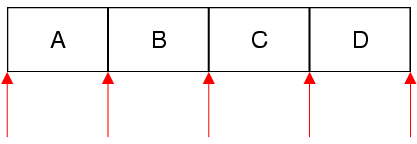
\includegraphics[width=0.5\textwidth]{javaiterators1}
\end{figure}

%%%%%%%%

下面的例子演示如何反序遍历元素:

\begin{lstlisting}[language=C++]
QMapIterator<int, QWidget *> i(map);
i.toBack();
while (i.hasPrevious()) {
    i.previous();
    qDebug() << i.key() << ": " << i.value();
\end{lstlisting}

如果想查找特定值的所有实例,循环使用 findNext() 或 findPrevious()。例如:

\begin{lstlisting}[language=C++]
QMapIterator<int, QWidget *> i(map);
while (i.findNext(widget)) {
    qDebug() << "Found widget " << widget << " under key "
             << i.key();
}
\end{lstlisting}

同一 map 可以使用多个迭代器。
如果在 QMapIterator 处于活动状态时修改 map,QMapIterator 将继续在原 map 上遍历,
而忽略修改后的副本。

\begin{notice}[另请参阅]
QMutableMapIterator 和 QMap::const\_iterator。
\end{notice}

%%%%%%%%%%%%%

\section{成员函数文档}

bool QMapIterator::findPrevious(const T \emph{\&value})

从当前迭代器位置开始向后查找值 \emph{value}。
如果找到值为 \emph{value} 的键值对,返回 true;
否则返回 false。

调用该函数后,如果找到值,迭代器将被移动到匹配元素的前面;
否则,迭代器将被移动到容器的前端。

\begin{notice}[另请参阅]
findNext()。
\end{notice}

\splitLine

bool QMapIterator::findNext(const T \emph{\&value})

从当前迭代器位置开始向前查找值 \emph{value}。
如果找到值为 \emph{value} 的键值对,返回 true;
否则返回 false。

调用该函数后,如果找到值 \emph{value},迭代器将被移动到匹配元素的后面;
否则,迭代器将被移动到容器的末端。

\begin{notice}[另请参阅]
findPrevious()。
\end{notice}
    
\splitLine

const Key \&QMapIterator::key() const

调用遍历函数(next(),previous(),findNext(),findPrevious())后,该函数返回跳过的最后一个元素的键。

调用 next() 或 findNext() 后,key() 与 peekPrevious().key() 相同。调用 previous() 或 findPrevious() 后,key() 与 peekNext().key() 相同。

\begin{notice}[另请参阅]
value()。
\end{notice}

\splitLine

QMapIterator::Item QMapIterator::peekPrevious() const

不移动迭代器而返回前一个元素。

对返回值调用 key() 获取元素的键,调用 value() 获取元素的值。

对位于容器前端的迭代器调用该函数将导致未定义结果。

\begin{notice}[另请参阅]
hasPrevious(),previous() 和 peekNext()。
\end{notice}

\splitLine

QMapIterator::Item QMapIterator::previous()

返回前一个元素并将迭代器向后移动一个位置。

对返回值调用 key() 获取元素的键,调用 value() 获取元素的值。

对位于容器前端的迭代器调用该函数将导致未定义结果。


\begin{notice}[另请参阅]
hasPrevious(),peekPrevious() 和 next()。
\end{notice}

\splitLine

bool QMapIterator::hasPrevious() const

如果该迭代器前面至少有一个元素,返回 true,即该迭代器不在容器的前端;否则返回 false。

\begin{notice}[另请参阅]
hasNext() 和 previous()。
\end{notice}

\splitLine

bool QMapIterator::hasNext() const

如果该迭代器后面至少有一个元素,返回 true,即该迭代器不在容器的末端;否则返回 false。

\begin{notice}[另请参阅]
hasPrevious() 和 next()。
\end{notice}

\splitLine

void QMapIterator::toBack()

将迭代器移动到容器的末端(最后一个元素之后)。

\begin{notice}[另请参阅]
toFront() 和 previous()。
\end{notice}

\splitLine

void QMapIterator::toFront()

将迭代器移动到容器的前端(第一个元素之前)。

\begin{notice}[另请参阅]
toBack() 和 next()。
\end{notice}

\splitLine

QMapIterator<Key, T> \&QMapIterator::operator=(const QMap<Key, T> \emph{\&container})

将迭代器关联到 \emph{container} 来遍历 map。迭代器将被移动到 map 的前端(第一个元素之前)。


\begin{notice}[另请参阅]
toFront() 和 toBack()。
\end{notice}

\splitLine

QMapIterator::QMapIterator(const QMap<Key, T> \emph{\&map})

构造一个迭代器来遍历 \emph{map}。迭代器将被移动到 \emph{map} 的前端(第一个元素之前)。


\begin{notice}[另请参阅]
operator=()。
\end{notice}

\splitLine

QMapIterator::Item QMapIterator::next()

返回下一个元素并将迭代器向前移动一个位置。

对返回值调用 key() 获取元素的键,调用 value() 获取元素的值。

对位于容器末端的迭代器调用该函数将导致未定义结果。

\begin{notice}[另请参阅]
hasNext(),peekNext() 和 previous()。
\end{notice}
    
\splitLine

QMapIterator::Item QMapIterator::peekNext() const

不移动迭代器而返回下一个元素。

对返回值调用 key() 获取元素的键,调用 value() 获取元素的值。

对位于容器末端的迭代器调用该函数将导致未定义结果。

\begin{notice}[另请参阅]
hasNext(),next() 和 peekPrevious()。
\end{notice}

\splitLine

const T \&QMapIterator::value() const

调用遍历函数(next(),previous(),findNext(),findPrevious())后,该函数返回跳过的最后一个元素的值。

调用 next() 或 findNext() 后,value() 与 peekPrevious().value() 相同。

调用 previous() 或 findPrevious() 后,value() 与 peekNext().value() 相同。

\begin{notice}[另请参阅]
key()。
\end{notice}
\chapter{QMetaClassInfo}

QMetaClassInfo 类提供了某个类的附加信息。更多内容...

\begin{tabular}{|r|l|}
	\hline
	属性 & 方法 \\
	\hline
	头文件 & \#include <QMetaClassInfo>\\      
	\hline
	qmake & QT += core\\      
	\hline
\end{tabular}

\section{公共成员函数}

\begin{tabular}{|r|l|}   
\hline
const char * 	&name() const \\
\hline
const char * 	& value() const \\ 
\hline
\end{tabular}

\section{详细描述}

类型信息对象指的在源代码中通过 Q\_CLASSINFO() 指定的名称-值对。
这些信息可以通过 name() 和 value() 获取,例如:

\begin{cppcode}
class MyClass
{
    Q_OBJECT
    Q_CLASSINFO("author", "Sabrina Schweinsteiger")
    Q_CLASSINFO("url", "http://doc.moosesoft.co.uk/1.0/")

public:
    ...
};
\end{cppcode}

此机制可以在您的应用中自由使用,Qt 不会在自身的任何类中使用它。

\begin{seeAlso}
QMetaObject。
\end{seeAlso}

\section{成员函数文档}

const char *QMetaClassInfo::name() const

返回本信息对象的名称。

\begin{seeAlso}
value()。
\end{seeAlso}

const char *QMetaClassInfo::value() const

返回本信息对象的值。

\begin{seeAlso}
name()。
\end{seeAlso}
\chapter{QMetaMethod}

QMetaMethod 类提供了对应一个成员函数的元数据。更多内容...

\begin{tabular}{|r|l|}
	\hline
	属性 & 方法 \\
	\hline
	头文件 & \#include <QMetaMethod>\\      
	\hline
	qmake & QT += core\\      
	\hline
\end{tabular}

\section{公共类型}

\begin{tabular}{|r|l|}   
\hline
类型	& 名称 \\ 
\hline
enum	&Access \{ Private, Protected, Public \} \\ 
\hline
enum	& MethodType \{ Method, Signal, Slot, Constructor \} \\
\hline
\end{tabular}

\section{公共成员函数}

\begin{longtable}[l]{|l|m{27em}|} 
\hline
返回类型 & 函数 \\   
\hline
QMetaMethod::Access	& access() const \\ 
\hline
bool &	invoke(QObject *object, Qt::ConnectionType connectionType, QGenericReturnArgument returnValue, QGenericArgument val0 = QGenericArgument(nullptr), QGenericArgument val1 = QGenericArgument(), QGenericArgument val2 = QGenericArgument(), QGenericArgument val3 = QGenericArgument(), QGenericArgument val4 = QGenericArgument(), QGenericArgument val5 = QGenericArgument(), QGenericArgument val6 = QGenericArgument(), QGenericArgument val7 = QGenericArgument(), QGenericArgument val8 = QGenericArgument(), QGenericArgument val9 = QGenericArgument()) const \\
\hline
bool &	invoke(QObject *object, QGenericReturnArgument returnValue, QGenericArgument val0 = QGenericArgument(0), QGenericArgument val1 = QGenericArgument(), QGenericArgument val2 = QGenericArgument(), QGenericArgument val3 = QGenericArgument(), QGenericArgument val4 = QGenericArgument(), QGenericArgument val5 = QGenericArgument(), QGenericArgument val6 = QGenericArgument(), QGenericArgument val7 = QGenericArgument(), QGenericArgument val8 = QGenericArgument(), QGenericArgument val9 = QGenericArgument()) const \\
\hline
bool &	invoke(QObject *object, Qt::ConnectionType connectionType, QGenericArgument val0 = QGenericArgument(0), QGenericArgument val1 = QGenericArgument(), QGenericArgument val2 = QGenericArgument(), QGenericArgument val3 = QGenericArgument(), QGenericArgument val4 = QGenericArgument(), QGenericArgument val5 = QGenericArgument(), QGenericArgument val6 = QGenericArgument(), QGenericArgument val7 = QGenericArgument(), QGenericArgument val8 = QGenericArgument(), QGenericArgument val9 = QGenericArgument()) const \\
\hline
bool &	invoke(QObject *object, QGenericArgument val0 = QGenericArgument(0), QGenericArgument val1 = QGenericArgument(), QGenericArgument val2 = QGenericArgument(), QGenericArgument val3 = QGenericArgument(), QGenericArgument val4 = QGenericArgument(), QGenericArgument val5 = QGenericArgument(), QGenericArgument val6 = QGenericArgument(), QGenericArgument val7 = QGenericArgument(), QGenericArgument val8 = QGenericArgument(), QGenericArgument val9 = QGenericArgument()) const \\
\hline
bool &	invokeOnGadget(void *gadget, QGenericReturnArgument returnValue, QGenericArgument val0 = QGenericArgument(nullptr), QGenericArgument val1 = QGenericArgument(), QGenericArgument val2 = QGenericArgument(), QGenericArgument val3 = QGenericArgument(), QGenericArgument val4 = QGenericArgument(), QGenericArgument val5 = QGenericArgument(), QGenericArgument val6 = QGenericArgument(), QGenericArgument val7 = QGenericArgument(), QGenericArgument val8 = QGenericArgument(), QGenericArgument val9 = QGenericArgument()) const \\
\hline
bool &	invokeOnGadget(void *gadget, QGenericArgument val0 = QGenericArgument(0), QGenericArgument val1 = QGenericArgument(), QGenericArgument val2 = QGenericArgument(), QGenericArgument val3 = QGenericArgument(), QGenericArgument val4 = QGenericArgument(), QGenericArgument val5 = QGenericArgument(), QGenericArgument val6 = QGenericArgument(), QGenericArgument val7 = QGenericArgument(), QGenericArgument val8 = QGenericArgument(), QGenericArgument val9 = QGenericArgument()) const \\
\hline
const char * 	&name() const \\
\hline
const char * 	& value() const \\ 
\hline
bool & 	isValid() const \\ 
\hline
int	& methodIndex() const \\ 
\hline
QByteArray &	methodSignature() const \\ 
\hline
QMetaMethod::MethodType	 & methodType() const \\
\hline
QByteArray & 	name() const \\ 
\hline
int	& parameterCount() const \\
\hline
QList<QByteArray>	& parameterNames() const \\
\hline
int	& parameterType(int index) const \\
\hline
QList<QByteArray> &	parameterTypes() const \\
\hline
int	& returnType() const \\
\hline
int	& revision() const \\ 
\hline
const char *	& tag() const \\ 
\hline
const char *	& typeName() const \\ 
\hline
\end{longtable}


\section{静态公共成员}


\begin{tabular}{|l|l|}
\hline
返回类型 &	函数 \\ 
\hline
QMetaMethod 	&fromSignal(PointerToMemberFunction \emph{signal}) \\ 
\hline
\end{tabular}

\section{相关非成员函数}

\begin{tabular}{|l|l|}
\hline
返回类型 &	函数 \\ 
\hline
bool  &	operator!=(const QMetaMethod \emph{\&m1}, const QMetaMethod \emph{\&m2}) \\
\hline 
bool  &	operator==(const QMetaMethod \emph{\&m1}, const QMetaMethod \emph{\&m2})  \\
\hline
\end{tabular}

\section{宏定义}

\begin{tabular}{|c|c|}
	\hline
	宏定义 \\ 
	\hline
Q\_METAMETHOD\_INVOKE\_MAX\_ARGS \\ 
	\hline
	\end{tabular}

\section{详细描述}

QMetaMethod 类具有一个 methodType()、一个 methodSignature()、一组 parameterTypes() 和 parameterNames()、返回值的 typeName()、一个 tag()、一个 access() 描述符。
可以通过 invoke() 来执行任意 QObject 的方法。

\begin{seeAlso}
QMetaObject、QMetaEnum、QMetaProperty 和 Qt 属性系统。
\end{seeAlso}

\section{成员类型文档}

enum QMetaMethod::Access

此枚举描述某方法的访问权限,遵循 C++ 相关公约。


\begin{tabular}{|c|c|}
	\hline
	常量 	& 数值  \\
	\hline
	QMetaMethod::Private  &	0 \\ 
	\hline
	QMetaMethod::Protected &	1 \\ 
	\hline
	QMetaMethod::Public &	2 \\ 
	\hline
	\end{tabular}

enum QMetaMethod::MethodType	

\begin{tabular}{|c|c|c|}
	\hline
	常量  &	数值 	& 描述  \\ 
	\hline
	QMetaMethod::Method &	0 &	该函数是普通的成员函数。 \\
	\hline
	QMetaMethod::Signal &	1 	&该函数是信号函数。 \\
	\hline
	QMetaMethod::Slot &	2 &	该函数是槽函数。 \\ 
	\hline
	QMetaMethod::Constructor &	3 &	该函数是构造函数。 \\ 
	\hline
	\end{tabular}

\section{成员函数文档}

QMetaMethod::Access QMetaMethod::access() const

返回该方法的访问权限(private、protected 或 `public)。

\begin{notice}
信号永远是公共的,但应将此认为是实现细节。在类外发射该类的信号通常是个坏主意。
\end{notice}

\begin{seeAlso}
methodType()。
\end{seeAlso}

[static] template <typename PointerToMemberFunction> QMetaMethod QMetaMethod::fromSignal(PointerToMemberFunction signal)

返回对应给定 signal 的元方法,若 signal 并非信号,则返回无效的 QMetaMethod 对象。

范例:

\begin{lstlisting}[language=C++]
QMetaMethod destroyedSignal = QMetaMethod::fromSignal(&QObject::destroyed);
\end{lstlisting}


本函数在 Qt 5.0 中被引入。

bool QMetaMethod::invoke(QObject *object, Qt::ConnectionType connectionType, QGenericReturnArgument returnValue, 
   QGenericArgument val0 = QGenericArgument(nullptr), 
   QGenericArgument val1 = QGenericArgument(), 
QGenericArgument val2 = QGenericArgument(), 
QGenericArgument val3 = QGenericArgument(), 
QGenericArgument val4 = QGenericArgument(), 
QGenericArgument val5 = QGenericArgument(), 
QGenericArgument val6 = QGenericArgument(), 
QGenericArgument val7 = QGenericArgument(),
 QGenericArgument val8 = QGenericArgument(), 
 QGenericArgument val9 = QGenericArgument()) const

通过 object 对象动态调用本方法。若可被动态调用则返回 tue,若该对象无此方法或参数不匹配则返回 false。

该动态调用可以是同步或异步的,由 connectionType 决定:

\begin{compactitem}[\arr]
\item 若 type 是 Qt::DirectConnection,则该方法会被立即执行。
\item 若 type 是 Qt::QueuedConnection,则会发送一个 QEvent ,该方法会在应用进入该对象所属线程的主事件循环后执行。
\item 若 type 是 Qt::AutoConnection,当 object 与调用者处于相同线程中时,该方法会被同步执行,否则会被异步执行。
\end{compactitem}

返回值会被存放在 returnvalue 中。若调用方式是异步,则返回值无法被获取。
最多可以传递十个参数 (val0, val1, val2, val3, val4, val5, val6, val7, val8 和 val9) 至本方法。

QGenericArgument 和 QGenericReturnArgument 是内部的辅助类。
为了动态调用信号槽,您需要将参数通过 Q\_ARG() 和 Q\_RETURN\_ARG() 宏进行封装。
Q\_ARG() 接受一个类型名称和一个该类型的不可变引用;
Q\_RETURN\_ARG() 接受一个类型名称和一个该类型的可变引用。

通过异步方式动态调用 QPushButton 的 animateClick() 槽:

\begin{lstlisting}[language=C++]
int methodIndex = pushButton->metaObject()->indexOfMethod("animateClick()");
QMetaMethod method = metaObject->method(methodIndex);
method.invoke(pushButton, Qt::QueuedConnection);
\end{lstlisting}

当异步调用方法时,传递的参数必须被 Qt 的元对象系统所知悉,因为 Qt 需要在后台事件中拷贝并保存它们。
如果您使用队列连接时遇到下述错误信息:

\begin{lstlisting}
QMetaMethod::invoke: Unable to handle unregistered datatype 'MyType'	
\end{lstlisting}

则在调用 invokeMethod() 之前通过 qRegisterMetaType() 来注册该数据类型。

若想通过 obj 对象同步调用 \hl{compute(QString, int, double)} 槽,则代码如下:

\begin{lstlisting}[language=C++]
QString retVal;
QByteArray normalizedSignature = QMetaObject::normalizedSignature("compute(QString, int, double)");
int methodIndex = obj->metaObject()->indexOfMethod(normalizedSignature);
QMetaMethod method = obj->metaObject()->method(methodIndex);
method.invoke(obj,
              Qt::DirectConnection,
              Q_RETURN_ARG(QString, retVal),
              Q_ARG(QString, "sqrt"),
              Q_ARG(int, 42),
              Q_ARG(double, 9.7));
\end{lstlisting}


此处使用了 QMetaObject::normalizedSignature() 来确保函数签名符合 invoke() 期望的格式,即将多余的空白移除。

若 compute 槽通过特定顺序没有完整获取到一个 QString、一个 int 和一个 double,则此调用会失败。

\begin{warning}
此方法不会验证参数的有效性,object 必须是创建 QMetaMethod 的 QMetaObject 的类型实例,参数列表必须与该方法的保持一直,否则会导致未定义行为。
\end{warning}

\begin{seeAlso}
Q\_ARG()、Q\_RETURN\_ARG()、qRegisterMetaType() 和 QMetaObject::invokeMethod()。
\end{seeAlso}


%%%%%%%%%

bool QMetaMethod::invoke(QObject *object, QGenericReturnArgument returnValue, QGenericArgument val0 = QGenericArgument(0), QGenericArgument val1 = QGenericArgument(), QGenericArgument val2 = QGenericArgument(), QGenericArgument val3 = QGenericArgument(), QGenericArgument val4 = QGenericArgument(), QGenericArgument val5 = QGenericArgument(), QGenericArgument val6 = QGenericArgument(), QGenericArgument val7 = QGenericArgument(), QGenericArgument val8 = QGenericArgument(), QGenericArgument val9 = QGenericArgument()) const

此函数是 invoke() 的重载。

此重载始终通过 Qt::AutoConnection 调用本方法。

bool QMetaMethod::invoke(QObject *object, Qt::ConnectionType connectionType, QGenericArgument val0 = QGenericArgument(0), QGenericArgument val1 = QGenericArgument(), QGenericArgument val2 = QGenericArgument(), QGenericArgument val3 = QGenericArgument(), QGenericArgument val4 = QGenericArgument(), QGenericArgument val5 = QGenericArgument(), QGenericArgument val6 = QGenericArgument(), QGenericArgument val7 = QGenericArgument(), QGenericArgument val8 = QGenericArgument(), QGenericArgument val9 = QGenericArgument()) const

此函数是 invoke() 的重载。

此重载用于不关心对返回值的场合。

bool QMetaMethod::invoke(QObject *object, QGenericArgument val0 = QGenericArgument(0), QGenericArgument val1 = QGenericArgument(), QGenericArgument val2 = QGenericArgument(), QGenericArgument val3 = QGenericArgument(), QGenericArgument val4 = QGenericArgument(), QGenericArgument val5 = QGenericArgument(), QGenericArgument val6 = QGenericArgument(), QGenericArgument val7 = QGenericArgument(), QGenericArgument val8 = QGenericArgument(), QGenericArgument val9 = QGenericArgument()) const

此函数是 invoke() 的重载。

此重载通过 Qt::AutoConnection 调用本方法,并忽略返回值。

bool QMetaMethod::invokeOnGadget(void \emph{*gadget}, QGenericReturnArgument \emph{returnValue}, QGenericArgument \emph{val0} = QGenericArgument(nullptr), QGenericArgument val1 = QGenericArgument(), QGenericArgument val2 = QGenericArgument(), QGenericArgument val3 = QGenericArgument(), QGenericArgument val4 = QGenericArgument(), QGenericArgument val5 = QGenericArgument(), QGenericArgument val6 = QGenericArgument(), QGenericArgument val7 = QGenericArgument(), QGenericArgument val8 = QGenericArgument(), QGenericArgument val9 = QGenericArgument()) const

通过 Q\_GADGET 对象动态调用本方法。
若可被动态调用则返回 tue,若该对象无此方法或参数不匹配则返回 false。

gadget 指针必须是 Q\_GADGET 类的实例。

该调用始终是同步的。

返回值会被存放在 returnvalue 中。若调用方式是异步,则返回值无法被获取。最多可以传递十个参数 (val0, val1, val2, val3, val4, val5, val6, val7, val8 和 val9) 至本方法。

\begin{seeAlso}
此方法不会验证参数的有效性,gadget 必须是创建 QMetaMethod 的 QMetaObject 的类型实例,参数列表必须与该方法的保持一直,否则会导致未定义行为。
\end{seeAlso}

本函数在 Qt 5.5 中被引入。

\begin{seeAlso}
Q\_ARG()、Q\_RETURN\_ARG()、qRegisterMetaType() 和 QMetaObject::invokeMethod()。
\end{seeAlso}

bool QMetaMethod::invokeOnGadget(void \*gadget, QGenericArgument val0 = QGenericArgument(0), QGenericArgument val1 = QGenericArgument(), QGenericArgument val2 = QGenericArgument(), QGenericArgument val3 = QGenericArgument(), QGenericArgument val4 = QGenericArgument(), QGenericArgument val5 = QGenericArgument(), QGenericArgument val6 = QGenericArgument(), QGenericArgument val7 = QGenericArgument(), QGenericArgument val8 = QGenericArgument(), QGenericArgument val9 = QGenericArgument()) const

这是一个重载函数。

此重载函数通过 gadget 对象动态调用本方法,并忽略返回值。

本函数在 Qt 5.5 中被引入。

bool QMetaMethod::isValid() const

若此方法有效则返回 true(即可被自省并动态调用),否则返回 false。

本函数在 Qt 5.0 中被引入。

int QMetaMethod::methodIndex() const

返回本方法的索引编号。

本函数在 Qt 4.6 中被引入。

QByteArray QMetaMethod::methodSignature() const

返回本方法的签名(例如 setValue(double))。

本函数在 Qt 5.0 中被引入。

\begin{seeAlso}
parameterTypes() 和 parameterNames()。
\end{seeAlso}

QMetaMethod::MethodType QMetaMethod::methodType() const

返回本方法的类型(signal、slot、method 或 constructor)。

\begin{seeAlso}
access()。
\end{seeAlso}

QByteArray QMetaMethod::name() const

返回本方法的名字。

本函数在 Qt 5.0 中被引入。

\begin{seeAlso}
methodSignature() 和 parameterCount()。
\end{seeAlso}

int QMetaMethod::parameterCount() const

返回本方法的参数个数。

本函数在 Qt 5.0 中被引入。

\begin{seeAlso}
parameterType() 和 parameterNames()。
\end{seeAlso}

QList<QByteArray> QMetaMethod::parameterNames() const

返回参数名称列表。

\begin{seeAlso}
parameterTypes() 和 methodSignature()。
\end{seeAlso}

int QMetaMethod::parameterType(int \emph{index}) const

返回对应 index 的参数类型。

返回值是 QMetaType 中注册的类型之一,若该类型未被注册则返回 QMetaType::UnknownType。

本函数在 Qt 5.0 中被引入。

\begin{seeAlso}
parameterCount()、returnType() 和 QMetaType。
\end{seeAlso}

QList<QByteArray> QMetaMethod::parameterTypes() const

返回参数类型的列表。

\begin{seeAlso}
parameterNames() 和 methodSignature()。
\end{seeAlso}

int QMetaMethod::returnType() const

返回本方法返回值的类型。

返回

返回值是 QMetaType 中注册的类型之一,若该类型未被注册则返回 QMetaType::UnknownType。

本函数在 Qt 5.0 中被引入。

\begin{seeAlso}
parameterType()、QMetaType 和 typeName()。
\end{seeAlso}

int QMetaMethod::revision() const

返回通过 Q\_REVISION 注明的版本,若未注明则返回 0。

本函数在 Qt 5.1 中被引入。

const char *QMetaMethod::tag() const

返回与本方法关联的标签。

标签在此处指的是可以被 moc 识别的特定宏,用于为方法添加附加信息。

标签信息可以用如下方式添加到函数声明中:

\begin{lstlisting}[language=C++]
// 在 MainWindow 类声明中
#ifndef Q_MOC_RUN
// 将标签内容定义为空,以确保对编译器不可见
#  define MY_CUSTOM_TAG
#endif
...
private slots:
	MY_CUSTOM_TAG void testFunc();
\end{lstlisting}

相关信息可通过如下方式获取:

\begin{lstlisting}[language=C++]
MainWindow win;
win.show();

int functionIndex = win.metaObject()->indexOfSlot("testFunc()");
QMetaMethod mm = win.metaObject()->method(functionIndex);
qDebug() << mm.tag(); // 将打印 MY_CUSTOM_TAG
\end{lstlisting}

%%%%%%%%

此时,moc 会提取并记录所有标签,但不会对它们做任何特殊处理。您可以用标签来标注不同的方法,并在您的应用中通过特定的用途来使用它们。

\begin{notice}
自 Qt 5.0 开始,moc 会展开预编译宏,所以必须将标签定义包含在 \#ifndef Q\_MOC\_RUN 中,正如上文范例。
这在 Qt 4 中不是必要的,但上述代码在 Qt 4 中同样也能生效。
\end{notice}

const char *QMetaMethod::typeName() const

返回本方法的返回类型名称。

\begin{seeAlso}
returnType() 和 QMetaType::type()。
\end{seeAlso}

\section{相关非成员函数}

bool operator!=(const QMetaMethod \emph{\&m1}, const QMetaMethod\emph{\&m2})

这是一个重载函数。

若 m1 与 m2 不相等则返回 true,否则返回 false。

本函数在 Qt 5.0 中被引入。

bool operator==(const QMetaMethod \emph{\&m1}, const QMetaMethod \emph{\&m2})

这是一个重载函数。

若 m1 与 m2 相等则返回 true,否则返回 false。

本函数在 Qt 5.0 中被引入。

\section{宏定义文档}

Q\_METAMETHOD\_INVOKE\_MAX\_ARGS

此宏的数值等于通过 QMetaMethod::invoke() 执行方法时,可以传递的最大参数个数。
\chapter{QMetaObject 结构体}

QMetaObject 类包含了 Qt 对象的元信息。更多内容...。

\begin{tabular}{|r|l|}
	\hline
	属性 & 方法 \\
	\hline
	头文件 & \#include <QMetaObject>\\      
	\hline
	qmake & QT += core\\      
	\hline
\end{tabular}

\section{公共成员类型}


\begin{tabular}{|r|l|}   
\hline
类型	& 名称 \\ 
\hline
class	& Connection \\ 
\hline
\end{tabular}


\section{公共成员函数}

\begin{longtable}{|r|m{28em}|}   
\hline
QMetaClassInfo	& classInfo(int \emph{index}) const \\ 
\hline
int &	classInfoCount() const \\
\hline
int	&classInfoOffset() const\\
\hline
const char *	&className() const\\
\hline
QMetaMethod	&constructor(int index) const\\
\hline
int	&constructorCount() const\\
\hline
QMetaEnum	&enumerator(int index) const\\
\hline
int	&enumeratorCount() const\\
\hline
int	&enumeratorOffset() const\\
\hline
int&	indexOfClassInfo(const char *name) const\\
\hline
int	&indexOfConstructor(const char *constructor) const\\
\hline
int	&indexOfEnumerator(const char *name) const\\
\hline
int	&indexOfMethod(const char *method) const\\
\hline
int	&indexOfProperty(const char *name) const\\
\hline
int	&indexOfSignal(const char *signal) const\\
\hline
int&	indexOfSlot(const char *slot) const\\
\hline
bool	&inherits(const QMetaObject *metaObject) const\\
\hline
QMetaMethod	&method(int index) const\\
\hline
int	&methodCount() const\\
\hline
int	&methodOffset() const\\
\hline
QObject *	&newInstance(QGenericArgument val0 = QGenericArgument(nullptr), QGenericArgument val1 = QGenericArgument(), QGenericArgument val2 = QGenericArgument(), QGenericArgument val3 = QGenericArgument(), QGenericArgument val4 = QGenericArgument(), QGenericArgument val5 = QGenericArgument(), QGenericArgument val6 = QGenericArgument(), QGenericArgument val7 = QGenericArgument(), QGenericArgument val8 = QGenericArgument(), QGenericArgument val9 = QGenericArgument()) const\\
\hline
QMetaProperty	&property(int index) const\\
\hline
int&	propertyCount() const\\
\hline
int	&propertyOffset() const\\
\hline
const QMetaObject *	&superClass() const\\
\hline
QMetaProperty	&userProperty() const\\
\hline
\end{longtable}



\section{静态公共成员}

\begin{longtable}{|l|m{28em}|}
\hline
返回类型 &	函数 \\ 
\hline
bool	&checkConnectArgs(const char *signal, const char *method) \\
\hline
bool	&checkConnectArgs(const QMetaMethod \&signal, const QMetaMethod \&method) \\
\hline
void	&connectSlotsByName(QObject *object) \\
\hline
bool	&invokeMethod(QObject *obj, const char *member, Qt::ConnectionType type, QGenericReturnArgument ret, QGenericArgument val0 = QGenericArgument(nullptr), QGenericArgument val1 = QGenericArgument(), QGenericArgument val2 = QGenericArgument(), QGenericArgument val3 = QGenericArgument(), QGenericArgument val4 = QGenericArgument(), QGenericArgument val5 = QGenericArgument(), QGenericArgument val6 = QGenericArgument(), QGenericArgument val7 = QGenericArgument(), QGenericArgument val8 = QGenericArgument(), QGenericArgument val9 = QGenericArgument())\\
\hline
bool	&invokeMethod(QObject *obj, const char *member, QGenericReturnArgument ret, QGenericArgument val0 = QGenericArgument(0), QGenericArgument val1 = QGenericArgument(), QGenericArgument val2 = QGenericArgument(), QGenericArgument val3 = QGenericArgument(), QGenericArgument val4 = QGenericArgument(), QGenericArgument val5 = QGenericArgument(), QGenericArgument val6 = QGenericArgument(), QGenericArgument val7 = QGenericArgument(), QGenericArgument val8 = QGenericArgument(), QGenericArgument val9 = QGenericArgument())\\
\hline
bool	&invokeMethod(QObject *obj, const char *member, Qt::ConnectionType type, QGenericArgument val0 = QGenericArgument(0), QGenericArgument val1 = QGenericArgument(), QGenericArgument val2 = QGenericArgument(), QGenericArgument val3 = QGenericArgument(), QGenericArgument val4 = QGenericArgument(), QGenericArgument val5 = QGenericArgument(), QGenericArgument val6 = QGenericArgument(), QGenericArgument val7 = QGenericArgument(), QGenericArgument val8 = QGenericArgument(), QGenericArgument val9 = QGenericArgument())\\
\hline
bool	&invokeMethod(QObject *obj, const char *member, QGenericArgument val0 = QGenericArgument(0), QGenericArgument val1 = QGenericArgument(), QGenericArgument val2 = QGenericArgument(), QGenericArgument val3 = QGenericArgument(), QGenericArgument val4 = QGenericArgument(), QGenericArgument val5 = QGenericArgument(), QGenericArgument val6 = QGenericArgument(), QGenericArgument val7 = QGenericArgument(), QGenericArgument val8 = QGenericArgument(), QGenericArgument val9 = QGenericArgument())\\
\hline
bool	&invokeMethod(QObject *context, Functor function, Qt::ConnectionType type = Qt::AutoConnection, FunctorReturnType *ret = nullptr) \\
\hline
bool	&invokeMethod(QObject *context, Functor function, FunctorReturnType *ret) \\
\hline
QByteArray&	normalizedSignature(const char *method) \\
\hline
QByteArray&	normalizedType(const char *type)\\
\hline
\end{longtable}

\section{宏定义}

\begin{tabular}{|l|l|}
\hline
返回类型	& 宏定义 \\
\hline
QGenericArgument	& Q\_ARG(Type, const Type \&value) \\
\hline
QGenericReturnArgument&	Q\_RETURN\_ARG(Type, Type \&value) \\
\hline
\end{tabular}



\section{详细描述}

Qt 的元对象系统负责信号槽跨对象通信机制、运行时类型信息和 Qt 的属性系统。
应用中的每个 QObject 子类都有一个唯一的 QMetaObject 实例(译者注:与类一一对应,即同一个 QObject 子类的任意对象,都使用同一个 QMetaObject),其中保存了这个 QObject 子类的所有元信息,可以通过 QObject::metaObject() 获取。

QMetaObject 在应用编写中通常不需要,但在进行元编程时会非常有用,例如脚本引擎或者用户界面生成器。

最常用的成员函数有:

\begin{compactitem}
\item className() 返回类的名称。
\item superClass() 返回父类对应的元对象。
\item method() 和 methodCount() 提供关于一个类的元方法(信号、槽和其它可动态调用的成员方法)。
\item enumerator() 和 enumeratorCount() 提供一个类的枚举类型的信息。
\item propertyCount() 和 property() 提供一个类的属性的信息。
\item constructor() 和 constructorCount() 提供一个类的元构造函数的信息。
\end{compactitem}


索引函数 indexOfConstructor()、indexOfMethod()、indexOfEnumerator() 和 indexOfProperty() 将构造函数、成员函数、枚举类型和属性的名称映射为索引。例如,当连接信号槽时,Qt 内部使用 indexOfMethod() 进行检索。

类可以拥有一系列 名称—数值 格式的附加信息,保存在 QMetaClassInfo 对象中。信息条目数量可通过 classInfoCount()查询, classInfo()返回单条信息,也可通过 indexOfClassInfo() 检索信息条目。

\begin{notice}
元对象系统的操作通常是线程安全的,比如元对象是在编译期生成的静态只读实例。
然而,如果元对象在被程序动态修改了(如通过 QQmlPropertyMap),应用需要显示地同步对相关对象的访问。
\end{notice}

\begin{seeAlso}
QMetaClassInfo、QMetaEnum、QMetaMethod、QMetaProperty、QMetaType 和 Meta-Object System。
\end{seeAlso}

\section{成员函数文档}

[static] bool QMetaObject::checkConnectArgs(const char \emph{*signal}, const char \emph{*method})

如果 signal 和 method 的参数能够匹配则返回 true,否则返回 false。

signal 和 method 都被假设是已经规范化的。

\begin{seeAlso}
normalizedSignature()。
\end{seeAlso}

[static] bool QMetaObject::checkConnectArgs(const QMetaMethod \emph{\&signal}, const QMetaMethod \emph{\&method})

这是一个重载函数。

如果 signal 和 method 的参数能够匹配则返回 true,否则返回 false。

本函数在 Qt 5.0 中被引入。

QMetaClassInfo QMetaObject::classInfo(int \emph{index}) const

返回对应 index 的类型信息的元数据对象。

范例:

\begin{cppcode}
class MyClass : public QObject
 {
     Q_OBJECT
     Q_CLASSINFO("author", "Sabrina Schweinsteiger")
     Q_CLASSINFO("url", "http://doc.moosesoft.co.uk/1.0/")

 public:
     ...
 };
\end{cppcode}


%%%%%%%%%%%%%%%%

\begin{seeAlso}
classInfoCount()、classInfoOffset() 和 indexOfClassInfo()。
\end{seeAlso}

int QMetaObject::classInfoCount() const

返回该类信息条目数量。

\begin{seeAlso}
classInfo()、classInfoOffset() 和 indexOfClassInfo()。
\end{seeAlso}

int QMetaObject::classInfoOffset() const

返回类信息在该类中的偏移量,即第一条类信息的编号。

若该类没有包含类信息的父类,则偏移量为 0,否则偏移量是所有父类的类信息数量的总和。

\begin{seeAlso}
classInfo()、classInfoCount() 和 indexOfClassInfo()。
\end{seeAlso}

const char *QMetaObject::className() const

返回该类的名称。

\begin{seeAlso}
superClass()。
\end{seeAlso}

[static] void QMetaObject::connectSlotsByName(QObject \emph{*object})

递归检索 \emph{object} 和所有子对象,将它们的信号连接至 object 中匹配的槽,匹配格式如下:

\begin{lstlisting}
void on_<对象名>_<信号名>(<信号参数>);
\end{lstlisting}

假设有一个对象名 为 button1 的 QPushButton 类型的子对象,则捕获它的 clicked() 信号的槽应为:

\begin{cppcode}
void on_button1_clicked();
\end{cppcode}

若 object 对象自身的名字已设置,则它自己的信号也会被连接至对应的槽。

\begin{seeAlso}
QObject::setObjectName().
\end{seeAlso}

%%%%%%%%%%%
QMetaMethod QMetaObject::constructor(int \emph{index}) const

返回指定 \emph{index} 的构造函数的元数据。

该函数在 Qt 4.5 中被引入。

\begin{seeAlso}
constructorCount() 和 newInstance()。
\end{seeAlso}

int QMetaObject::constructorCount() const

返回此类的构造函数个数。

该函数在 Qt 4.5 中被引入。

\begin{seeAlso}
constructor() 和 indexOfConstructor()。
\end{seeAlso}

QMetaEnum QMetaObject::enumerator(int \emph{index}) const

返回指定 \emph{index} 的枚举类型的元数据。

\begin{seeAlso}
enumeratorCount()、enumeratorOffset() 和 indexOfEnumerator()。
\end{seeAlso}

int QMetaObject::enumeratorCount() const

返回该类的枚举类型的个数。

\begin{seeAlso}
enumerator()、enumeratorOffset() 和 indexOfEnumerator()。
\end{seeAlso}
	
int QMetaObject::enumeratorOffset() const

返回该类的枚举类型偏移量,即首个枚举变量的编号。

若该类没有包含枚举类型的父类,则偏移量为 0,否则偏移量是所有父类的枚举类型数量的总和。

\begin{seeAlso}
enumerator()、enumeratorCount() 和 indexOfEnumerator()。
\end{seeAlso}

int QMetaObject::indexOfClassInfo(const char \emph{*name}) const

查找名为 \emph{name} 的类型信息条目并返回其编号,未找到则返回-1。

\begin{seeAlso}
classInfo()、classInfoCount() 和 classInfoOffset()。
\end{seeAlso}

int QMetaObject::indexOfConstructor(const char \emph{*constructor}) const

查找名为 \emph{constructor} 的构造函数并返回其编号,未找到则返回-1。

\begin{notice}
constructor 需要为规范化的格式,如 normalizedSignature() 的返回值。
\end{notice}

该函数在 Qt 4.5 中被引入。

\begin{seeAlso}
constructor()、constructorCount() 和 normalizedSignature()。
\end{seeAlso}

int QMetaObject::indexOfEnumerator(const char \emph{*name}) const

查找名为 \emph{name} 的枚举类型并返回其编号,未找到则返回-1。

\begin{notice}
enumerator(), enumeratorCount() 和 enumeratorOffset().
\end{notice}

int QMetaObject::indexOfMethod(const char \emph{*method}) const

查找名为 \emph{method} 的方法并返回其编号,未找到则返回-1。

\begin{notice}
method 需要为规范化的格式,如 normalizedSignature() 的返回值。
\end{notice}

\begin{seeAlso}
method()、methodCount()、methodOffset() 和 normalizedSignature()。
\end{seeAlso}

int QMetaObject::indexOfProperty(const char \emph{*name}) const

查找名为 name 的属性并返回其编号,未找到则返回-1。

\begin{seeAlso}
property()、propertyCount() 和 propertyOffset()。	
\end{seeAlso}

int QMetaObject::indexOfSignal(const char \emph{*signal}) const

查找名为 name 的信号并返回其编号,未找到则返回-1。

此方法与 indexOfMethod() 相似,区别是若该方法存在但并非信号函数,则会返回 -1。

\begin{notice}
signal 需要为规范化的格式,如 normalizedSignature() 的返回值。	
\end{notice}

\begin{seeAlso}
indexOfMethod()、normalizedSignature(), method()、methodCount() 和 methodOffset()。
\end{seeAlso}

int QMetaObject::indexOfSlot(const char \emph{*slot}) const

查找名为 name 的槽并返回其编号,未找到则返回-1。

此方法与 indexOfMethod() 相似,区别是若该方法存在但并非槽函数,则会返回 -1。

\begin{seeAlso}
indexOfMethod()、method()、methodCount() 和 methodOffset()。
\end{seeAlso}

bool QMetaObject::inherits(const QMetaObject \emph{*metaObject}) const

若该 QMetaObject 继承自 \emph{metaObject} 描述的类型,则返回 true,否则返回 false。

一个类型被认为是继承自它自己的。

该函数在 Qt 5.7 中被引入。

%%%%%%
[static] bool QMetaObject::invokeMethod(QObject *obj, const char *member, 
 Qt::ConnectionType type, QGenericReturnArgument ret, 
 QGenericArgument val0 = QGenericArgument(nullptr), QGenericArgument val1 = QGenericArgument(), 
 QGenericArgument val2 = QGenericArgument(),QGenericArgument val3 = QGenericArgument(), 
 QGenericArgument val4 = QGenericArgument(), QGenericArgument val5 = QGenericArgument(), 
 QGenericArgument val6 = QGenericArgument(), QGenericArgument val7 = QGenericArgument(), 
 QGenericArgument val8 = QGenericArgument(), QGenericArgument val9 = QGenericArgument())

通过 obj 对象动态调用它的 member 方法(或者信号和槽),若调用成功则返回 true,若该对象没有此方法或参数不匹配则返回 false。

该调用可以是同步或异步的,由 type 决定:

\begin{compactitem}
\item 若 type 是 Qt::DirectConnection,则该方法会被立即执行。
\item 若 type 是 Qt::QueuedConnection,则会发送一个 QEvent ,该方法会在应用进入该对象所属线程的主事件循环后执行。
\item 若 type 是 Qt::BlockingQueuedConnection,则该方法会通过与 Qt::QueuedConnection 相同的方式执行,
	此外当前线程会被阻塞,直到该事件被响应。使用此方法在相同线程的对象间通信会导致死锁。
\item 若 type 是 Qt::AutoConnection,当 obj 与调用者处于相同线程中时,该方法会被同步执行,否则会被异步执行。
\end{compactitem}

member 函数的返回值会被存放在 ret 中。若调用方式是异步,则返回值无法被获取。最多可以传递十个参数 (val0, val1, val2, val3, val4, val5, val6, val7, val8 和 val9) 至 member 函数。

QGenericArgument 和 QGenericReturnArgument 是内部的辅助类。为了动态调用信号槽,您需要将参数通过 Q\_ARG() 和 Q\_RETURN\_ARG() 宏进行封装。
Q\_ARG() 接受一个类型名称和一个该类型的不可变引用;
Q\_RETURN\_ARG() 接受一个类型名称和一个该类型的可变引用。

您只需要将信号槽的名称传递至本函数,无需传递完整的签名。

例如,异步调用某个 QThread 对象的 quit() 槽需要的代码如下:

\begin{cppcode}
QMetaObject::invokeMethod(thread, "quit",
                           Qt::QueuedConnection);
\end{cppcode}

当异步调用方法时,传递的参数必须被 Qt 的元对象系统所知悉,因为 Qt 需要在后台事件中拷贝并保存它们。
如果您使用队列连接时遇到下述错误信息:

\begin{lstlisting}
QMetaObject::invokeMethod: Unable to handle unregistered datatype 'MyType'
\end{lstlisting}

则在调用 invokeMethod() 之前通过 qRegisterMetaType() 来注册该数据类型。

若想通过 obj 对象同步调用 compute(QString, int, double) 槽,则代码如下:

\begin{cppcode}
 QString retVal;
 QMetaObject::invokeMethod(obj, "compute", Qt::DirectConnection,
                           Q_RETURN_ARG(QString, retVal),
                           Q_ARG(QString, "sqrt"),
                           Q_ARG(int, 42),
                           Q_ARG(double, 9.7));
\end{cppcode}

若 compute 槽通过特定顺序没有完整获取到一个 QString、一个 int 和一个 double,则此调用会失败。

\begin{notice}
此方法是线程安全的。
\end{notice}

\begin{seeAlso}
Q\_ARG()、Q\_RETURN\_ARG()、qRegisterMetaType() 和 QMetaMethod::invoke()。
\end{seeAlso}

%%%%%%%%%%%

[static] bool QMetaObject::invokeMethod(QObject \emph{*obj}, const char \emph{*member}, QGenericReturnArgument \emph{ret}, 
QGenericArgument val0 = QGenericArgument(0), QGenericArgument val1 = QGenericArgument(), 
QGenericArgument val2 = QGenericArgument(), 
QGenericArgument val3 = QGenericArgument(), QGenericArgument val4 = QGenericArgument(), 
QGenericArgument val5 = QGenericArgument(), QGenericArgument val6 = QGenericArgument(), 
QGenericArgument val7 = QGenericArgument(), QGenericArgument val8 = QGenericArgument(), 
QGenericArgument val9 = QGenericArgument())

此函数是 invokeMethod() 的重载。

此重载始终通过 Qt::AutoConnection 调用对应方法。

\begin{notice}
此方法是线程安全的。
\end{notice}

[static] bool QMetaObject::invokeMethod(QObject *obj, const char *member, Qt::ConnectionType type, QGenericArgument val0 = QGenericArgument(0), QGenericArgument val1 = QGenericArgument(), QGenericArgument val2 = QGenericArgument(), QGenericArgument val3 = QGenericArgument(), QGenericArgument val4 = QGenericArgument(), QGenericArgument val5 = QGenericArgument(), QGenericArgument val6 = QGenericArgument(), QGenericArgument val7 = QGenericArgument(), QGenericArgument val8 = QGenericArgument(), QGenericArgument val9 = QGenericArgument())

此函数是 invokeMethod() 的重载。

此重载用于不关心对返回值的场合。


\begin{notice}
此方法是线程安全的。
\end{notice}


[static] bool QMetaObject::invokeMethod(QObject \emph{*obj}, const char \emph{*member}, 
 QGenericArgument val0 = QGenericArgument(0), QGenericArgument val1 = QGenericArgument(),
  QGenericArgument val2 = QGenericArgument(), QGenericArgument val3 = QGenericArgument(),
   QGenericArgument val4 = QGenericArgument(), QGenericArgument val5 = QGenericArgument(), 
   QGenericArgument val6 = QGenericArgument(), QGenericArgument val7 = QGenericArgument(), 
   QGenericArgument val8 = QGenericArgument(), QGenericArgument val9 = QGenericArgument())

此函数是 invokeMethod() 的重载。

此重载通过 Qt::AutoConnection 调用对应方法,并忽略返回值。

\begin{notice}
此方法是线程安全的。
\end{notice}

[static] template <typename Functor, typename FunctorReturnType> bool QMetaObject::invokeMethod(QObject \emph{*context}, Functor \emph{function}, Qt::ConnectionType \emph{type} = Qt::AutoConnection, FunctorReturnType \emph{*ret} = nullptr)

此函数是 invokeMethod() 的重载。

通过 type 方式在 \emph{context} 所属的事件循环中动态调用 \emph{function}。\emph{function} 可以是一个仿函数或成员函数指针。
若该函数可被动态调用则返回 true,当该函数不存在或参数不匹配时返回 false。函数的返回值将被保存至 \emph{ret} 中。

\begin{notice}
此方法是线程安全的。
\end{notice}

该函数在 Qt 5.10 中被引入。

[static] template <typename Functor, typename FunctorReturnType> bool QMetaObject::invokeMethod(QObject \emph{*context}, Functor \emph{function}, FunctorReturnType \emph{*ret})

此函数是 invokeMethod() 的重载。

通过 Qt::AutoConnection 方式动态调用 \emph{function}。\emph{function} 可以是一个仿函数或成员函数指针。
若该函数可被动态调用则返回 true,当该函数不存在或参数不匹配时返回 false。函数的返回值将被保存至 \emph{ret} 中。


\begin{notice}
此方法是线程安全的。
\end{notice}


该函数在 Qt 5.10 中被引入。

QMetaMethod QMetaObject::method(int \emph{index}) const

返回指定 \emph{index} 的方法的元数据。

\begin{seeAlso}
methodCount(), methodOffset() 和 indexOfMethod().
\end{seeAlso}

int QMetaObject::methodCount() const

返回该类中方法的数量,包括所有基类的方法个数。除了常规成员函数外,也包含信号函数和槽函数。

使用下述代码来将所给类的所有方法签名存储至 QStringList:

\begin{cppcode}
 const QMetaObject* metaObject = obj->metaObject();
 QStringList methods;
 for(int i = metaObject->methodOffset(); i < metaObject->methodCount(); ++i)
     methods << QString::fromLatin1(metaObject->method(i).methodSignature());
\end{cppcode}

\begin{seeAlso}
method()、methodOffset() 和 indexOfMethod()。
\end{seeAlso}

int QMetaObject::methodOffset() const

返回类方法在该类中的偏移量,即第一个类方法的编号。

该偏移量是所有父类的方法数总和(因此总为正数,因为 QObject 有 deleteLater() 槽和 destroyed() 信号)。

\begin{seeAlso}
method()、methodCount() 和 indexOfMethod()。
\end{seeAlso}

QObject *QMetaObject::newInstance(QGenericArgument \emph{val0} = QGenericArgument(nullptr), QGenericArgument \emph{val1} = QGenericArgument(), 
    QGenericArgument \emph{val2} = QGenericArgument(), QGenericArgument \emph{val3} = QGenericArgument(), 
    QGenericArgument \emph{val4} = QGenericArgument(), QGenericArgument \emph{val5} = QGenericArgument(), 
    QGenericArgument \emph{val6} = QGenericArgument(), QGenericArgument \emph{val7} = QGenericArgument(), 
    QGenericArgument \emph{val8} = QGenericArgument(), QGenericArgument \emph{val9} = QGenericArgument()) const

构造一个此类的新实例。您可以传递最多十个参数 (val0, val1, val2, val3, val4, val5, val6, val7, val8 和 val9) 至构造函数。返回构造的新对象,若没有合适的构造函数则返回 nullptr。

\begin{notice}
只有通过 Q\_INVOKABLE 修饰符声明的构造函数才能在元对象系统中使用。
\end{notice}

该函数在 Qt 4.5 中被引入。

\begin{seeAlso}
Q\_ARG() 和 constructor()。
\end{seeAlso}

[static] QByteArray QMetaObject::normalizedSignature(const char \emph{*method})

将给予的 \emph{method} 进行规范化。

Qt 使用规范化的签名来来判断两个给定的信号和槽是否匹配。
规范化操作会将空格减到最少,将 const 适当前移,移除值类型的 const,并将不可变引用替换为值类型。

\begin{seeAlso}
checkConnectArgs() 和 normalizedType()。
\end{seeAlso}

[static] QByteArray QMetaObject::normalizedType(const char \emph{*type})

将 \emph{type} 规范化。

请参阅 QMetaObject::normalizedSignature() 中关于 Qt 如何进行规范化的描述。

范例:

\begin{cppcode}
 QByteArray normType = QMetaObject::normalizedType(" int    const  *");
 // 规范化的类型将为 "const int*"
\end{cppcode}

%%%%%%%%%%%%%%%%%%

该函数在 Qt 4.2 中被引入。

\begin{seeAlso}
normalizedSignature()。
\end{seeAlso}

QMetaProperty QMetaObject::property(int \emph{index}) const

返回指定 \emph{index} 的属性的元数据。
若该属性不存在,则返回空的 QMetaProperty 对象。

\begin{seeAlso}
propertyCount()、propertyOffset() 和 indexOfProperty()。
\end{seeAlso}

int QMetaObject::propertyCount() const

返回该类中属性的类型,包括所有基类的属性个数。

使用如下代码来将给定类的所有属性名称保存至 QStringList: 

\begin{cppcode}
 const QMetaObject* metaObject = obj->metaObject();
 QStringList properties;
 for(int i = metaObject->propertyOffset(); i < metaObject->propertyCount(); ++i)
     properties << QString::fromLatin1(metaObject->property(i).name());
\end{cppcode}

\begin{seeAlso}
property()、propertyOffset() 和 indexOfProperty()。
\end{seeAlso}

int QMetaObject::propertyOffset() const

返回类属性在该类中的偏移量,即第一条类属性的编号。

该偏移量包含所有父类的类属性数量总和(因此总为正数,因为 QObject 有 name() 属性)。

\begin{seeAlso}
property()、propertyCount() 和 indexOfProperty()。
\end{seeAlso}

const QMetaObject *QMetaObject::superClass() const

返回父类的元对象,若不存在则返回 \hl{nullptr}。

\begin{seeAlso}
className()。
\end{seeAlso}

QMetaProperty QMetaObject::userProperty() const

返回 \hl{USER} 标志位为 \hl{true} 的元属性。

该函数在 Qt 4.2 中被引入。

\begin{seeAlso}
QMetaProperty::isUser()。
\end{seeAlso}

\section{宏定义文档}

QGenericArgument Q\_ARG(Type, const Type \emph{\&value})

该宏接受一个 \hl{type} 和一个该类型的 \hl{value} 参数,

返回一个用于传递至 QMetaObject::invokeMethod() 的 QGenericArgument 对象。

\begin{seeAlso}
Q\_RETURN\_ARG()。
\end{seeAlso} 

QGenericReturnArgument Q\_RETURN\_ARG(\emph{Type}, Type \emph{\&value})

该宏接受一个 \hl{Type} 和一个该类型的可变引用 \hl{value} 参数,

返回一个用于传递至 QMetaObject::invokeMethod() 的包含该类型的 QGenericReturnArgument 对象。

\begin{seeAlso}
Q\_ARG()。
\end{seeAlso} 
\chapter{Connection}

QMetaObject::Connection 类。

\section{公共成员函数}

\begin{tabular}{|r|l|}
	\hline
返回类型  &	函数 \\ 
\hline
	&Connection(Connection \emph{\&\&o}) \\ 
    \hline
	&Connection(const Connection \emph{\&other}) \\ 
    \hline
	&Connection() \\ 
    \hline
Connection & 	operator=(Connection \emph{\&\&other}) \\ 
\hline
Connection & 	operator=(const Connection \emph{\&other}) \\
	& $\sim$Connection() \\ 
    \hline
bool &	operator bool() const    \\ 
	\hline
\end{tabular}


\section{详细描述}

代表一组信号槽(或信号-仿函数)连接的句柄。

此类可被用于检查连接是否有效,或通过 QObject::disconnect() 断开连接。
对于不具备上下文对象的 信号-仿函数 连接,这是唯一的断开连接的方式。

由于 Connection 仅仅是一个句柄,当被销毁或重新赋值时,底层的信号槽连接不会被影响。

\section{成员函数文档}

Connection::Connection(Connection \emph{\&\&o})

移动构造函数,将其指向 \hl{o} 原先指向的对象。

Connection::Connection(const Connection \emph{\&other})

生成 \hl{other} 连接的句柄的一份拷贝。

Connection::Connection()

创建一个空的连接实例。

Connection \&Connection::operator=(Connection \emph{\&\&other})

将 \hl{other} 转移赋值至本对象,并返回本对象的引用。

Connection \&Connection::operator=(const Connection \emph{\&other})

将 \hl{other} 赋值给本对象,并返回本对象的引用。

Connection::$\sim$Connection()

QMetaObject::Connection 的析构函数。

bool Connection::operator bool() const

若该对象有效,则返回 \hl{true}。

若 QObject::connect 成功,则该连接是有效的;
若 QObject::connect 无法找到对应的信号槽或参数不匹配,则该连接无效。
\chapter{QMetaProperty}

QMetaProperty 类提供了对应一条属性的元数据。更多内容...

\begin{tabular}{|r|l|}
	\hline
	属性 & 方法 \\
	\hline
    头文件  &	\hl{\#include <QMetaProperty>} \\
    \hline
    qmake: & \hl{QT += core}    \\
	\hline
\end{tabular}

\section{公共成员函数}

\begin{longtable}{|r|m{28em}|}   
\hline
返回类型 	& 函数 \\
\hline
QMetaEnum &	enumerator() const \\
\hline 
bool &	hasNotifySignal() const \\ 
\hline
bool &	isConstant() const \\ 
\hline
bool &	isDesignable(const QObject \emph{*object} = nullptr) const \\
\hline
bool &	isEnumType() const \\
\hline
bool 	&isFinal() const \\ 
\hline
bool 	&isFlagType() const \\ 
\hline
bool &	isReadable() const \\ 
\hline
bool &	isRequired() const\\
\hline
bool &	isResettable() const\\
\hline
bool &	isScriptable(const QObject \emph{*object} = nullptr) const\\
\hline
bool 	&isStored(const QObject \emph{*object} = nullptr) const\\
\hline
bool 	&isUser(const QObject \emph{*object} = nullptr) const\\
\hline
bool &	isValid() const\\
\hline
bool 	&isWritable() const\\
\hline
const char * &	name() const\\
\hline
QMetaMethod &	notifySignal() const\\
\hline
int 	& notifySignalIndex() const\\
\hline
int  &	propertyIndex() const\\
\hline
QVariant &	read(const QObject \emph{*object}) const \\
\hline
QVariant 	&readOnGadget(const void \emph{*gadget}) const \\
\hline
int 	&relativePropertyIndex() const\\
\hline
bool &	reset(QObject \emph{*object}) const\\
\hline
bool 	&resetOnGadget(void \emph{*gadget}) const \\
\hline
int 	&revision() const\\
\hline
QVariant::Type &	type() const \\
\hline
const char * &	typeName() const \\ 
\hline
int 	& userType() const \\ 
\hline
bool &	write(QObject \emph{*object}, const QVariant \emph{\&value}) const \\ 
\hline
bool 	&writeOnGadget(void \emph{*gadget}, const QVariant \emph{\&value}) const \\ 
\hline
\end{longtable}


\section{详细描述}

属性元数据可通过对象的元对象获取。详见 QMetaObject::property() 和 QMetaObject::propertyCount()。

\subsection{属性元数据}

属性具有 name() 和 type(),并且有不同的成员来表示其外在表现: isReadable()、isWritable()、isDesignable()、
isScriptable()、revision() 和 isStored()。

若该属性是枚举变量,则 isEnumType() 返回 true;
若该属性是枚举,同时也是标志位(即可通过或运算合并多个值),
则 isEnumType() 和 isFlagType() 都返回 true。这些类型的枚举值可以通过 enumerator() 查询。

属性的值通过 read()、write() 和 reset()来获取或设置,也可以通过 QObject 的 get 和 set 函数来操作,
详见 QObject::setProperty() 和 QObject::property()。

\subsection{拷贝与赋值}

QMetaProperty 对象可以通过传值方式拷贝,与此同时,每份副本内部都会指向相同的属性元数据。

\begin{seeAlso}
QMetaObject,QMetaEnum,QMetaMethod 和 Qt 属性系统。
\end{seeAlso}

\section{成员函数文档}

QMetaEnum QMetaProperty::enumerator() const

若该属性是枚举类型,则返回对应的枚举器,否则返回未定义值。

\begin{seeAlso}
isEnumType() 和 isFlagType()。
\end{seeAlso}

bool QMetaProperty::hasNotifySignal() const

若该属性有对应的通知信号则返回 true,否则返回 false。

\begin{seeAlso}
notifySignal()。
\end{seeAlso}

bool QMetaProperty::isConstant() const

若该属性在 Q\_PROPERTY() 中被标记为 CONSTANT 则返回 true,否则返回 false。

本函数在 Qt 4.6 中被引入。

bool QMetaProperty::isDesignable(const QObject \emph{*object} = nullptr) const

若该属性可被设计师(Qt Designer)编辑则返回 true,否则返回 false。

若 object 未被指定,则当 Q\_PROPERTY() 的 DESIGNABLE 标记被指定为 false时,此函数返回 false ;其它情况下返回 true(若该标记被指定为 true,或指定为某个函数,或指定为表达式)。

\begin{seeAlso}
isScriptable() 和 isStored()。
\end{seeAlso}

bool QMetaProperty::isEnumType() const

若该属性是枚举类型则返回 true,否则返回 false。

\begin{seeAlso}
enumerator() 和 isFlagType()。
\end{seeAlso}

bool QMetaProperty::isFinal() const

若该属性在 Q\_PROPERTY() 中被标记为 FINAL 则返回 true,否则返回 false。

本函数在 Qt 4.6 中被引入。

bool QMetaProperty::isFlagType() const

若该属性是标志位则返回 true,否则返回 false。

标志位可以通过或运算合并多个值。标志位通常也是枚举类型。

\begin{seeAlso}
isEnumType(),enumerator() 和 QMetaEnum::isFlag()。
\end{seeAlso}

bool QMetaProperty::isReadable() const

若该属性可被读取则返回 true,否则返回 false。

\begin{seeAlso}
isWritable(),read() 和 isValid()。
\end{seeAlso}

bool QMetaProperty::isRequired() const

若该属性在 Q\_PROPERTY() 中被标记为 REQUIRED 则返回 true,否则返回 false。

本函数在 Qt 5.15 中被引入。

bool QMetaProperty::isResettable() const

若该属性可被重置为默认值则返回 true,否则返回 false。

\begin{seeAlso}
reset()。
\end{seeAlso}

bool QMetaProperty::isScriptable(const QObject \emph{*object} = nullptr) const

若该属性可被脚本化则返回 true,否则返回 false。

若 object 未被指定,则当 Q\_PROPERTY() 的 SCRIPTABLE 标记被指定为 false时,此函数返回 false ;
其它情况下返回 true(若该标记被指定为 true,或指定为某个函数,或指定为表达式)。

\begin{seeAlso}
isDesignable() 和 isStored()。
\end{seeAlso}

bool QMetaProperty::isStored(const QObject *object = nullptr) const

若该属性可存储则返回 true,否则返回 false。

若 object 未被指定,则当 Q\_PROPERTY() 的 STORED 标记被指定为 false时,此函数返回 false ;其它情况下返回 true(若该标记被指定为 true,或指定为某个函数,或指定为表达式)。

\begin{seeAlso}
isDesignable() 和 isScriptable()。
\end{seeAlso}

bool QMetaProperty::isUser(const QObject *object = nullptr) const

若该属性被设计为 USER 性质则返回 true,即可以在 object 中被用户编辑,或在某些方面很重要;其它情况下返回 false。例如,QLineEdit 的 text 属性是 USER 可编辑的。

若 object 是 nullptr,则当 Q\_PROPERTY() 的 STORED 标记被指定为 false时,此函数返回 false ;
其它情况下返回 true。

\begin{seeAlso}
QMetaObject::userProperty(),isDesignable() 和 isScriptable()。
\end{seeAlso}

bool QMetaProperty::isValid() const

若该属性是有效的(可读)则返回 true,否则返回 false。

\begin{seeAlso}
isReadable()。
\end{seeAlso}

bool QMetaProperty::isWritable() const

若该属性可被写入则返回 true,否则返回 false。

\begin{seeAlso}
isReadable() 和 write()。
\end{seeAlso}

const char *QMetaProperty::name() const

返回本属性的名称。

\begin{seeAlso}
type() 和 typeName()。
\end{seeAlso}

QMetaMethod QMetaProperty::notifySignal() const

若已为本属性指定数值修改时发送的通知信号,则返回该通知信号对应的 QMetaMethod 实例,否则返回无效的 QMetaMethod 对象。

本函数在 Qt 4.5 中被引入。

\begin{seeAlso}
hasNotifySignal()。
\end{seeAlso}

int QMetaProperty::notifySignalIndex() const

若已为本属性指定数值修改时发送的通知信号,则返回该通知信号的索引编号,否则返回 -1。

本函数在 Qt 4.6 中被引入。

\begin{seeAlso}
hasNotifySignal()。
\end{seeAlso}

int QMetaProperty::propertyIndex() const

返回本属性的索引编号。

本函数在 Qt 4.6 中被引入。

QVariant QMetaProperty::read(const QObject *object) const

读取给定的 object 中的本属性,若可以读取则返回属性值,否则返回无效的 QVariant。

\begin{seeAlso}
write(),reset() 和 isReadable()。
\end{seeAlso}

QVariant QMetaProperty::readOnGadget(const void *gadget) const

读取给定的 gadget 中的本属性,若可以读取则返回属性值,否则返回无效的 QVariant。

当且仅当本属性是 Q\_GADGET 中的属性时,才可使用此函数。

本函数在 Qt 5.5 中被引入。

int QMetaProperty::relativePropertyIndex() const

返回本属性在对应的元对象中的相对索引编号。

本函数在 Qt 5.14 中被引入。

bool QMetaProperty::reset(QObject *object) const

通过重置方法重置给定的 object 中的本属性。若重置成功则返回 true,否则返回 false。

重置方法是可选的,只有少量属性支持重置。

\begin{seeAlso}
read() 和 write()。
\end{seeAlso}

bool QMetaProperty::resetOnGadget(void *gadget) const

通过重置方法重置给定的 gadget 中的本属性。若重置成功则返回 true,否则返回 false。

重置方法是可选的,只有少量属性支持重置。

当且仅当本属性是 Q\_GADGET 中的属性时,才可使用此函数。

本函数在 Qt 5.5 中被引入。

int QMetaProperty::revision() const

若该属性被 REVISION 标记,则返回对应的版本,否则返回 0。

本函数在 Qt 5.1 中被引入。

QVariant::Type QMetaProperty::type() const

返回本属性的类型。返回值是 QVariant::Type 的枚举值之。

\begin{seeAlso}
userType(),typeName() 和 name()。
\end{seeAlso}

const char *QMetaProperty::typeName() const

返回本属性的类型名称。

\begin{seeAlso}
type() 和 name()。
\end{seeAlso}

int QMetaProperty::userType() const

返回本属性的用户类型。返回值是 QMetaType 中注册的类型之一,若该类型未被注册则返回 QMetaType::UnknownType。

本函数在 Qt 4.2 中被引入。

\begin{seeAlso}
type(),QMetaType 和 typeName()。
\end{seeAlso}

bool QMetaProperty::write(QObject \emph{*object}, const QVariant \emph{\&value}) const

将 value 写入到给定的 object 的本属性中,若写入成功则返回 true,否则返回 false。

若 value 与本属性类型不一致,则会尝试进行自动转换。若本属性是可重置的,则传入空的 QVariant() 等价于调用 reset(),否则等价于设置为默认值。

\begin{seeAlso}
read(),reset() 和 isWritable()。
\end{seeAlso}

bool QMetaProperty::writeOnGadget(void \emph{*gadget}, const QVariant \emph{\&value}) const

将 value 写入到给定的 gadget 的本属性中,若写入成功则返回 true,否则返回 false。

当且仅当本属性是 Q\_GADGET 中的属性时,才可使用此函数。

本函数在 Qt 5.5 中被引入。
\chapter{QMetaType}

QMetaType 类管理元对象系统中的注名类型。更多内容...

\begin{tabular}{|r|l|}
	\hline
	属性 & 方法 \\
	\hline
    头文件  &	\hl{\#include <QMetaType>} \\
    \hline
    qmake: & \hl{QT += core}    \\
	\hline
\end{tabular}

\begin{notice}
此类中所有函数都是线程安全的。
\end{notice}

\section{公共成员类型}

\begin{tabular}{|r|m{25em}|}   
\hline
类型 	& 名称 \\
\hline
enum &	Type \{ Void, Bool, Int, UInt, Double, ..., UnknownType \} \\
\hline
enum &	TypeFlag \{ NeedsConstruction, NeedsDestruction, MovableType, IsEnumeration, PointerToQObject \}\\
\hline
flags &	TypeFlags\\
\hline
\end{tabular}

\section{公共成员函数}

\begin{longtable}{|r|m{28em}|}   
\hline
返回类型 	& 函数 \\
\hline
& QMetaType(const int \emph{typeId} = QMetaType::UnknownType) \\ 
\hline
& $\sim$QMetaType() \\
\hline
void *	&construct(void \emph{*where}, const void \emph{*copy} = 0) const \\
\hline
void *	&create(const void \emph{*copy} = 0) const \\
\hline
void	&destroy(void \emph{*data}) const \\
\hline
void	&destruct(void \emph{*data}) const \\
\hline
QMetaType::TypeFlags &	flags() const \\
\hline
int	& id() const \\ 
\hline
bool	&isRegistered() const \\
\hline
bool	&isValid() const \\
\hline
const QMetaObject *	& metaObject() const \\
\hline
::QByteArray &	name() const \\
\hline
int	& sizeOf() const \\
\hline
\end{longtable}

\section{静态公共成员}

\begin{longtable}{|r|m{28em}|}   
\hline
返回类型 	& 函数 \\
\hline
bool	& compare(const void \emph{*lhs}, const void \emph{*rhs}, int \emph{typeId}, int \emph{*result})\\
\hline
void *	&construct(int \emph{type}, void \emph{*where}, const void \emph{*copy})\\
\hline
bool	& convert(const void \emph{*from}, int \emph{fromTypeId}, void \emph{*to}, int \emph{toTypeId})\\
\hline
void *	& create(int \emph{ype}, const void \emph{*copy} = nullptr)\\
\hline
bool	& debugStream(QDebug \emph{\&dbg}, const void \emph{*rhs}, int \emph{typeId})\\
\hline
void	& destroy(int \emph{type}, void \emph{*data})\\
\hline
void	& destruct(int \emph{type}, void \emph{*where})\\
\hline
bool	&equals(const void \emph{*lhs}, const void \emph{*rhs}, int \emph{typeId}, int \emph{*result})\\
\hline
QMetaType&	fromType()\\
\hline
bool	& hasRegisteredComparators()\\
\hline
bool	& hasRegisteredComparators(int \emph{typeId})\\
\hline
bool	&hasRegisteredConverterFunction(int \emph{fromTypeId}, int \emph{toTypeId})\\
\hline
bool	&hasRegisteredConverterFunction()\\
\hline
bool	&hasRegisteredDebugStreamOperator()\\
\hline
bool	&hasRegisteredDebugStreamOperator(int \emph{typeId})\\
\hline
bool	&load(QDataStream  \emph{\&stream}, int  \emph{type}, void \emph{*data})\\
\hline
const QMetaObject *&	metaObjectForType(int \emph{type})\\
\hline
bool&	registerComparators()\\
\hline
bool&	registerConverter()\\
\hline
bool&	registerConverter(MemberFunction \emph{function})\\
\hline
bool&	registerConverter(MemberFunctionOk \emph{function})\\
\hline
bool&	registerConverter(UnaryFunction \emph{function})\\
\hline
bool&	registerDebugStreamOperator()\\
\hline
bool&	registerEqualsComparator()\\
\hline
bool&	save(QDataStream \emph{\&stream}, int \emph{type}, const void \emph{*data}) \\
\hline
int	&sizeOf(int \emph{type}) \\
\hline
int	& type(const char  \emph{*typeName}) \\
\hline
int	 & type(const ::QByteArray \emph{\&typeName}) \\
\hline
QMetaType::TypeFlags &	typeFlags(int \emph{type}) \\
\hline
const char * &	typeName(int \emph{typeId}) \\
\hline
\end{longtable}


\section{相关非成员函数}

\begin{tabular}{|r|m{25em}|}   
\hline
返回类型 	& 函数 \\
\hline
int &	qMetaTypeId()  \\ 
\hline
int &	qRegisterMetaType(const char \emph{*typeName}) \\ 
\hline
int	 & qRegisterMetaType() \\ 
\hline
void &	qRegisterMetaTypeStreamOperators(const char \emph{*typeName}) \\ 
\hline
bool &	operator!=(const QMetaType \emph{\&a}, const QMetaType \emph{\&b}) \\ 
\hline
bool &	operator==(const QMetaType \emph{\&a}, const QMetaType \emph{\&b}) \\ 
\hline
\end{tabular}

\section{宏定义}

\begin{tabular}{|l|}   
\hline
宏定义 \\
\hline
Q\_DECLARE\_ASSOCIATIVE\_CONTAINER\_METATYPE(\emph{Container}) \\
\hline
Q\_DECLARE\_METATYPE(\emph{Type}) \\
\hline
Q\_DECLARE\_OPAQUE\_POINTER(\emph{PointerType}) \\
\hline
Q\_DECLARE\_SEQUENTIAL\_CONTAINER\_METATYPE(\emph{Container}) \\ 
\hline
Q\_DECLARE\_SMART\_POINTER\_METATYPE(\emph{SmartPointer})\\
\hline
\end{tabular}


\section{详细描述}

此类是一个辅助类,被用作序列化 QVariant 以及队列连接信号槽中的类型。
它将类型名称关联到对应类型,以支持运行时动态创建和销毁此类型。
通过 Q\_DECLARE\_METATYPE() 声明新类型,让它可以被 QVariant 和其它模板函数(qMetaTypeId() 等)使用。
调用 qRegisterMetaType() 来让其可以被非模板型函数使用,如信号槽的队列连接。

任何包含一个公共默认构造函数、一个公共拷贝构造函数、一个默认析构函数的类或结构体都可以被注册为元类型。

下述代码展示了如何分配和销毁一个 MyClass 的实例:

\begin{cppcode}
int id = QMetaType::type("MyClass");
if (id != QMetaType::UnknownType) {
    void *myClassPtr = QMetaType::create(id);
    ...
    QMetaType::destroy(id, myClassPtr);
    myClassPtr = 0;
}
\end{cppcode}

若我们想让流运算符 operator<<() 和 operator>>() 可被用于存储了自定义类型的 QVariant 对象,则这个自定义类型必须提供 operator<<() 和 operator>>() 运算符重载。

\begin{seeAlso}
Q\_DECLARE\_METATYPE(),QVariant::setValue(),QVariant::value() 和 QVariant::fromValue().
\end{seeAlso}

\section{成员类型文档}

enum QMetaType::Type

下表是 QMetaType 内置支持的类型:


\begin{longtable}{|l|l|m{20em}|}   
\hline
常量 &	数值 &	描述 \\ 
\hline
QMetaType::Void &	43&	void \\
\hline
QMetaType::Bool	&1&	bool \\
\hline
QMetaType::Int	&2&	int \\
\hline
QMetaType::UInt	&3	&unsigned int \\
\hline
QMetaType::Double&	6	&double \\
\hline
QMetaType::QChar&	7	&QChar \\
\hline
QMetaType::QString	&10&	QString \\
\hline
QMetaType::QByteArray&	12&	QByteArray \\
\hline
QMetaType::Nullptr&	51&	std::nullptr\_t \\
\hline
QMetaType::VoidStar	&31&	void * \\
\hline
QMetaType::Long	&32	&long \\
\hline
QMetaType::LongLong	&4	&long long \\
\hline
QMetaType::Short	&33&	short \\
\hline
QMetaType::Char&	34	&char \\
\hline
QMetaType::ULong	&35	&unsigned long \\
\hline
QMetaType::ULongLong&	5	&unsigned long long \\
\hline
QMetaType::UShort&	36&	unsigned short \\
\hline
QMetaType::SChar&	40&	signed char \\
\hline
QMetaType::UChar&	37&	unsigned char \\
\hline
QMetaType::Float	&38&	float \\
\hline
QMetaType::QObjectStar	&39&	QObject * \\
\hline
QMetaType::QVariant	&41	&QVariant \\
\hline
QMetaType::QCursor	&74&	QCursor \\
\hline
QMetaType::QDate&	14	&QDate \\
\hline
QMetaType::QSize&	21&	QSize \\
\hline
QMetaType::QTime&	15	&QTime\\
\hline
QMetaType::QVariantList&	9	&QVariantList\\
\hline
QMetaType::QPolygon&	71	&QPolygon\\
\hline
QMetaType::QPolygonF&	86&	QPolygonF\\
\hline
QMetaType::QColor	&67&	QColor\\
\hline
QMetaType::QColorSpace&	87&	QColorSpace(在 Qt 5.15 中被引入)\\
\hline
QMetaType::QSizeF	&22	&QSizeF\\
\hline
QMetaType::QRectF	&20	&QRectF\\
\hline
QMetaType::QLine	&23	&QLine\\
\hline
QMetaType::QTextLength	&77&	QTextLength\\
\hline
QMetaType::QStringList	&11&	QStringList\\
\hline
QMetaType::QVariantMap	&8&	QVariantMap\\
\hline
QMetaType::QVariantHash	&28&	QVariantHash\\
\hline
QMetaType::QIcon&	69&	QIcon\\
\hline
QMetaType::QPen	&76	&QPen \\
\hline
QMetaType::QLineF	&24&	QLineF\\
\hline
QMetaType::QTextFormat&	78&	QTextFormat \\
\hline
QMetaType::QRect&	19	&QRect \\
\hline
QMetaType::QPoint&	25	&QPoint \\
\hline
QMetaType::QUrl	&17	&QUrl \\
\hline
QMetaType::QRegExp	&27	&QRegExp \\
\hline
QMetaType::QRegularExpression	&44	&QRegularExpression \\
\hline
QMetaType::QDateTime	&16&	QDateTime\\
\hline
QMetaType::QPointF	&26&	QPointF\\
\hline
QMetaType::QPalette	&68	&QPalette\\
\hline
QMetaType::QFont	&64&	QFont\\
\hline
QMetaType::QBrush	&66	&QBrush\\
\hline
QMetaType::QRegion&	72&	QRegion\\
\hline
QMetaType::QBitArray&	13	&QBitArray\\
\hline
QMetaType::QImage	&70	&QImage\\
\hline
QMetaType::QKeySequence	&75	&QKeySequence\\
\hline
QMetaType::QSizePolicy&	121&	QSizePolicy\\
\hline
QMetaType::QPixmap&	65	&QPixmap\\
\hline
QMetaType::QLocale&	18	&QLocale\\
\hline
QMetaType::QBitmap&	73&	QBitmap\\
\hline
QMetaType::QMatrix&	79&	QMatrix\\
\hline
QMetaType::QTransform	&80	&QTransform\\
\hline
QMetaType::QMatrix4x4	&81	&QMatrix4x4\\
\hline
QMetaType::QVector2D	&82	&QVector2D\\
\hline
QMetaType::QVector3D	&83	&QVector3D\\
\hline
QMetaType::QVector4D	&84	&QVector4D\\
\hline
QMetaType::QQuaternion&	85	&QQuaternion\\
\hline
QMetaType::QEasingCurve	&29&	QEasingCurve\\
\hline
QMetaType::QJsonValue	&45&	QJsonValue\\
\hline
QMetaType::QJsonObject&	46&	QJsonObject\\
\hline
QMetaType::QJsonArray	&47	&QJsonArray\\
\hline
QMetaType::QJsonDocument	&48&	QJsonDocument\\
\hline
QMetaType::QCborValue	&53&	QCborValue\\
\hline
QMetaType::QCborArray	&54	&QCborArray \\
\hline
QMetaType::QCborMap	&55&	QCborMap \\
\hline
QMetaType::QCborSimpleType	&52&	QCborSimpleType \\
\hline
QMetaType::QModelIndex&	42	&QModelIndex \\
\hline
QMetaType::QPersistentModelIndex&	50	&QPersistentModelIndex(在 Qt 5.5 中被引入) \\
\hline
QMetaType::QUuid	&30	&QUuid \\
\hline
QMetaType::QByteArrayList&	49&	QByteArrayList \\
\hline
QMetaType::User	&1024&	用户类型的基础值(译者注:即起始值)\\
\hline
QMetaType::UnknownType&	0	&这是无效的类型编号,QMetaType 会在类型未注册时返回此值。\\
\hline
\end{longtable}

可以使用 Q\_DECLARE\_METATYPE() 注册额外的类型。

\begin{seeAlso}
type() 和 typeName()。
\end{seeAlso}

\splitLine

enum QMetaType::TypeFlag

flags QMetaType::TypeFlags

此枚举类型描述了被 QMetaType 支持的类型的属性

\begin{tabular}{|l|l|l|}
\hline
常量 	&数值 &	描述\\
\hline
QMetaType::NeedsConstruction &	0x1 &	此类型具有非平凡的构造函数。若某类型不具备此标志,则可通过 memset() 安全地清零。\\
\hline
QMetaType::NeedsDestruction &	0x2 	&此类型非平凡的析构函数。若某类型不具备此标志,则丢弃对象前不需要调用析构函数(译者注:即可以用 free() 释放对象)\\
\hline
QMetaType::MovableType &	0x4 &	具有此标志的类型实例可以通过 memcpy() 安全地移动。\\
\hline
QMetaType::IsEnumeration 	&0x10 &	此类型是枚举值。\\
\hline
QMetaType::PointerToQObject &	0x8 &	此类型是指向继承自 QObject 的类型的指针。\\
\hline
\end{tabular}

\hl{TypeFlags} 类型是 QFlags<TypeFlag> 的别名,支持通过或操作合并不同的 \hl{TypeFlag} 值。

\section{成员函数文档}

QMetaType::QMetaType(const int typeId = QMetaType::UnknownType)

构造一个包含 typeId 对应的类型信息的 QMetaType 对象。

注意: 默认参数在 Qt 5.15 中被引入。

此函数在 Qt 5.0 中被引入。

QMetaType::$\sim$QMetaType()

析构此对象。

[static] bool QMetaType::compare(const void \emph{*lhs}, const void \emph{*rhs}, int typeId, int \emph{*result})

比较 lhs 和 rhs 对象,双方都需要是 typeid 中的类型。result 会被设为小于、等于或大于零,表示 lhs 小于、等于或大于 rhs。若比较成功则返回 true,否则返回 false。

此函数在 Qt 5.2 中被引入。

[static] void *QMetaType::construct(int \emph{type}, void \emph{*where}, const void \emph{*copy})

在给定的内存地址 where 上构造对应 type 类型的对象,该对象是 copy 的副本,并返回 where。若 copy 是空指针,则执行默认构造。

这是用于显示管理存储 type 类型对象的内存的底层函数。若不需要此类底层控制,则考虑使用 create() 函数(也就是指,使用 new 而非 placement new)。

您必须确保 where 指向的内存区域大小足够存储 type 对应的数据,并且 where 地址需要对齐,对应类型的大小可通过 sizeOf() 获取。

内存对齐的规则是对齐至类型的自然边界,也就是大于等于类型大小的2的n次方值,直至平台有效对齐宽度上限为止。对于特定用途来说,超过 2 * sizeof(void*) 的对齐宽度只是某些特定硬件指令所必需的(例如,x86 平台中对齐后的 SSE 读取和存储)。

此函数在 Qt 5.0 中被引入。

\begin{seeAlso}
destruct() 和 sizeOf()。
\end{seeAlso}

void *QMetaType::construct(void \emph{*where}, const void \emph{*copy} = 0) const

在给定的内存地址 where 上构造此 QMetaType 类型的对象,
该对象是 copy 的副本,并返回 where。
若 copy 是空指针,则执行默认构造。

这是用于显示管理存储 type 类型对象的内存的底层函数。
若不需要此类底层控制,则考虑使用 create() 函数(也就是指,使用 new 而非 placement new)。

您必须确保 where 指向的内存区域大小足够存储 type 对应的数据,
并且 where 地址需要对齐,对应类型的大小可通过 sizeOf() 获取。

内存对齐的规则是对齐至类型的自然边界,也就是大于等于类型大小的2的n次方值
,直至平台有效对齐宽度上限为止。对于特定用途来说,超过 2 * sizeof(void*) 的对齐宽度只是某些特定硬件指令所必需的(例如,x86 平台中对齐后的 SSE 读取和存储)。

此函数在 Qt 5.0 中被引入。

[static] bool QMetaType::convert(const void \emph{*from}, int \emph{fromTypeId}, void \emph{*to}, int \emph{toTypeId})

将 from 对象从 fromTypeId 转换至 toTypeId 并存储到预分配空间 to 中。若转换成功则返回 true,否则返回 false。

此函数在 Qt 5.2 中被引入。

[static] void *QMetaType::create(int \emph{type}, const void \emph{*copy} = nullptr)

假设 copy 的类型是 type,返回它的的拷贝。若 copy 是空指针,则返回默认构造的实例。

\begin{seeAlso}
destroy(),isRegistered() 和 Type。
\end{seeAlso}

void *QMetaType::create(const void \emph{*copy} = 0) const

假设 copy 的类型是此 QMetaType ,返回它的的拷贝。若 copy 是空指针,则返回默认构造的实例。

此函数在 Qt 5.0 中被引入。

\begin{seeAlso}
QMetaType::destroy()。
\end{seeAlso}

[static] bool QMetaType::debugStream(QDebug \emph{\&dbg}, const void \emph{*rhs}, int \emph{typeId})

将 typeId 类型的 rhs 对象输出至调试流 debug,输出成功则返回 true,否则返回 false。

此函数在 Qt 5.2 中被引入。

[static] void QMetaType::destroy(int \emph{type}, void \emph{*data})

假设 data 的类型是 type,销毁该对象。

\begin{seeAlso}
create(),isRegistered() 和 Type。
\end{seeAlso}

void QMetaType::destroy(void \emph{*data}) const

假设 data 的类型是此 QMetaType ,销毁该对象。

此函数在 Qt 5.0 中被引入。

\begin{seeAlso}
QMetaType::create()。
\end{seeAlso}

[static] void QMetaType::destruct(int \emph{type}, void \emph{*where})

假设 where 地址中存储的对象类型是 type,销毁该对象。

与 destroy() 不同,此函数只会执行该类型的析构函数,但不会执行 delete 运算符(译者注:即不会释放内存,与 placement new 相同机制)。

此函数在 Qt 5.0 中被引入。

\begin{seeAlso}
construct()。
\end{seeAlso}

void QMetaType::destruct(void \emph{*data}) const

假设 data 地址中存储的对象类型是此 QMetaType ,销毁该对象。

与 destroy() 不同,此函数只会执行该类型的析构函数,但不会执行 delete 运算符(译者注:即不会释放内存,与 placement new 相同机制)。

此函数在 Qt 5.0 中被引入。

\begin{seeAlso}
QMetaType::construct()。
\end{seeAlso}

[static] bool QMetaType::equals(const void \emph{*lhs}, const void \emph{*rhs}, int \emph{typeId}, int \emph{*result})

比较 lhs 和 rhs 对象,双方都需要是 typeid 中的类型。若 lhs 等于 rhs,则 result 会被设为零。若比较成功则返回 true,否则返回 false。

此函数在 Qt 5.5 中被引入。

QMetaType::TypeFlags QMetaType::flags() const

返回此 QMetaType 实例的类型标志。

此函数在 Qt 5.0 中被引入。

\begin{seeAlso}
QMetaType::TypeFlags 和 QMetaType::typeFlags()。
\end{seeAlso}

[static] template <typename T> QMetaType QMetaType::fromType()

返回模板类型 T 对应的 QMetaType 实例。

此函数在 Qt 5.15 中被引入。

[static] template <typename T> bool QMetaType::hasRegisteredComparators()

若模板类型 T 已被注册至元对象系统则返回 true。

此函数在 Qt 5.2 中被引入。

[static] bool QMetaType::hasRegisteredComparators(int \emph{typeId})

若 typeId 的类型已被注册至元对象系统则返回 true。

此函数在 Qt 5.2 中被引入。

[static] bool QMetaType::hasRegisteredConverterFunction(int \emph{fromTypeId}, int \emph{toTypeId})

若自 fromTypeId 到 toTypeId 的类型转换已被注册至元对象系统则返回 true。

此函数在 Qt 5.2 中被引入。

[static] template <typename From, typename To> bool QMetaType::hasRegisteredConverterFunction()

若自模板类型 From 到 To 的类型转换已被注册至元对象系统则返回 true。

这是一个重载函数。

此函数在 Qt 5.2 中被引入。

[static] template <typename T> bool QMetaType::hasRegisteredDebugStreamOperator()

若自模板类型 T 的 QDebug 流运算符已被注册至元对象系统则返回 true。

此函数在 Qt 5.2 中被引入。

[static] bool QMetaType::hasRegisteredDebugStreamOperator(int \emph{typeId})

若自 typeId 对应类型的 QDebug 流运算符已被注册至元对象系统则返回 true。

此函数在 Qt 5.2 中被引入。

int QMetaType::id() const

返回此 QMetatype 实例的类型编号。

此函数在 Qt 5.13 中被引入。

[static] bool QMetaType::isRegistered(int \emph{type})

若 typeId 对应已被注册至元对象系统则返回 true,否则返回 false。

\begin{seeAlso}
type(),typeName() 和 Type。
\end{seeAlso}

bool QMetaType::isRegistered() const

若此 QMetaType 包含某类型的有效信息则返回 true,否则返回 false。

此函数在 Qt 5.0 中被引入。

bool QMetaType::isValid() const

若此 QMetaType 包含某类型的有效信息则返回 true,否则返回 false。

此函数在 Qt 5.0 中被引入。

[static] bool QMetaType::load(QDataStream \emph{\&stream}, int \emph{type}, void \emph{*data})

从数据流 stream 中读取对应 type 类型的对象至 data 中,若读取成功则返回 true,否则返回 false。

此类型必须在这之前通过 qRegisterMetaType() 和 qRegisterMetaTypeStreamOperators() 完成注册。

通常来说,您不需要显示调用此函数,而是应使用 QVariant 的 operator>>(),该运算符依赖 load() 来传递自定义类型。

\begin{seeAlso}
save() 和 qRegisterMetaTypeStreamOperators()。
\end{seeAlso}

const QMetaObject *QMetaType::metaObject() const

返回此类型对应的 QMetaObject。

若此类型是 QObject 子类的指针,即 flags() 包含 QMetaType::PointerToQObject,则此函数会返回对应类型的 QMetaObject。这可被用于结合 QMetaObject::construct(译者注:无此函数,请使用 QMetaObject::constructor 或 QMetaType::construct)来创建此类型的 QObject 实例。

若此类型是 Q\_GADGET,即 flags() 包含 QMetaType::IsGadget(译者注:文档中未给出,但 QMetaType::TypeFlag 中的确包含此枚举值),则此函数会返回对应类型的 QMetaObject。
这可以被用于获取 QMetaMethod 和 QMetaProperty,并将其用于此类型的对象指针上(例如通过 QVariant::data 获取指针 译者注:文档中无此函数,但此函数的确存在)。

若此类型是枚举,即 flags() 包含 QMetaType::IsEnumeration,
且该枚举值是通过 Q\_ENUM 注册的成员枚举类型,
则此函数会返回其所属的 QObject 对象的元对象,否则返回 nullptr。

此函数在 Qt 5.5 中被引入。

\begin{seeAlso}
QMetaType::metaObjectForType() 和 QMetaType::flags()。
\end{seeAlso}

[static] const QMetaObject *QMetaType::metaObjectForType(int \emph{type})

返回 type 类型对应的 QMetaType::metaObject。

此函数在 Qt 5.0 中被引入。

\begin{seeAlso}
metaObject()。
\end{seeAlso}

QByteArray QMetaType::name() const

返回此 QMetaType 对应的类型名称,若无有效类型则返回空指针。

此函数在 Qt 5.15 中被引入。

\begin{seeAlso}
typeName()。
\end{seeAlso}

[static] template <typename T> bool QMetaType::registerComparators()

将用户注册类型 T 的比较运算符注册至元对象系统。要求 T 具有 operator== 和 operator< 运算符。若注册成功则返回 true,否则返回 false。

此函数在 Qt 5.2 中被引入。

[static] template <typename From, typename To> bool QMetaType::registerConverter()

将类型 From 到 To 的可能的隐式转换注册到元对象系统,若注册成功则返回 true,否则返回 false。

此函数在 Qt 5.2 中被引入。

[static] template <typename MemberFunction, int> bool QMetaType::registerConverter(MemberFunction \emph{function})

这是一个重载函数。

将形如 To From::function() const 的成员方法 function 作为从 From 到 To 的转换函数注册至元对象系统,若注册成功则返回 true,否则返回 false。

此函数在 Qt 5.2 中被引入。

\begin{quote}
译者注:

第二个模板参数是官方使用 doxygen 生成文档时的变通写法,
实际代码中的函数签名是 \hl{template<typename From, typename To> static bool registerConverter(To(From::*function)() const)}。
使用时无需指定 \hl{int} 模板参数,在函数参数中直接填入用于转换的成员函数指针即可。
\end{quote}

[static] template <typename MemberFunctionOk, char> bool QMetaType::registerConverter(MemberFunctionOk \emph{function})

这是一个重载函数。

将形如 To From::function(bool *ok) const 的成员方法 function 作为从 From 到 To 的转换函数注册至元对象系统,若注册成功则返回 true,否则返回 false。

此函数在 Qt 5.2 中被引入。

\begin{quote}
译者注:

第二个模板参数是官方使用 doxygen 生成文档时的变通写法,
实际代码中的函数签名是 \hl{template<typename From, typename To> static bool registerConverter(To(From::*function)(bool*) const)}。
使用时无需指定 \hl{char} 模板参数,在函数参数中直接填入用于转换的成员函数指针即可。
\end{quote}


[static] template <typename UnaryFunction> bool QMetaType::registerConverter(UnaryFunction \emph{function})

这是一个重载函数。

将把类型 From 转换为类型 To 的一元函数 function 注册至元对象系统,若注册成功则返回 true,否则返回 false。

此函数在 Qt 5.2 中被引入。

\begin{quote}
译者注:

原文描述地非常晦涩,实际指的是任何可被 \hl{To dst = function(src)} 方式调用的函数对象,
包括全局函数、类静态函数、仿函数或 lamba 等,比上文另外两个 \hl{registerConverter} 的约束更为宽松。
\end{quote}


%%%%%%%%%%%%%%%%
[static] template <typename T> bool QMetaType::registerDebugStreamOperator()

将已注册类型 T 的 QDebug 流运算符注册至元对象系统,
要求类型 T 具备流运算符 operator<<(QDebug dbg, T)。
若注册成功则返回 true,否则返回 false。

[static] template <typename T> bool QMetaType::registerEqualsComparator()

将已注册类型 T 的等号运算符注册至元对象系统,要求类型 T 具备等号运算符 operator==。
若注册成功则返回 true,否则返回 false。

此函数在 Qt 5.5 中被引入。

[static] bool QMetaType::save(QDataStream \emph{\&stream}, int \emph{type}, const void \emph{*data})

从数据流 stream 中读取对应 type 类型的对象至 data 中,若读取成功则返回 true,否则返回 false。

此类型必须在这之前通过 qRegisterMetaType() 和 qRegisterMetaTypeStreamOperators() 完成注册。

通常来说,您不需要显示调用此函数,而是应使用 QVariant 的 operator>>(),
该运算符依赖 load() 来传递自定义类型。

\begin{seeAlso}
save() 和 qRegisterMetaTypeStreamOperators()。
\end{seeAlso}

将 type 类型对应的 data 对象输出至数据流 stream 中,若读取成功则返回 true,否则返回 false。

此类型必须在这之前通过 qRegisterMetaType() 和 qRegisterMetaTypeStreamOperators() 完成注册。

通常来说,您不需要显示调用此函数,而是应使用 QVariant 的 operator<<(),
该运算符依赖 save() 来传递自定义类型。

\begin{seeAlso}
load() 和 qRegisterMetaTypeStreamOperators()。
\end{seeAlso}

[static] int QMetaType::sizeOf(int \emph{type})

返回 type 对应类型的以字节为单位的大小(即 sizeof(T),其中 T 是 type 对应的实际类型)。

此函数通常结合 construct() 使用,来进行对此类型的更底层的内存管理。

此函数在 Qt 5.0 中被引入。

\begin{seeAlso}
construct()。
\end{seeAlso}

int QMetaType::sizeOf() const

返回此类型的以字节为单位的大小(即 sizeof(T),其中 T 是 QMetaType 对应的实际类型)。

此函数通常结合 construct() 使用,来进行对此类型的更底层的内存管理。

此函数在 Qt 5.0 中被引入。

\begin{seeAlso}
QMetaType::construct() 和 QMetaType::sizeOf()。
\end{seeAlso}

[static] int QMetaType::type(const char \emph{*typeName})

返回名为 typeName 的类型的元类型编号,若无此元类型则返回 QMetaType::UnknownType。

\begin{seeAlso}
isRegistered(),typeName() 和 Type。
\end{seeAlso}

[static] int QMetaType::type(const::QByteArray \emph{\&typeName})

这是一个重载函数。

返回名为 typeName 的类型的元类型编号,若无此元类型则返回 0(译者注:即QMetaType::UnknownType)。

此函数在 Qt 5.5 中被引入。

\begin{seeAlso}
isRegistered() 和 typeName()。
\end{seeAlso}

[static] QMetaType::TypeFlags QMetaType::typeFlags(int \emph{type})

返回 type 类型的类型标志。

此函数在 Qt 5.0 中被引入。

\begin{seeAlso}
QMetaType::TypeFlags。
\end{seeAlso}

[static] const char *QMetaType::typeName(int \emph{typeId})

返回 typeId 对应类型的类型名称,若该类型不存在则返回空指针。返回的指针不可被删除。

\begin{seeAlso}
type(),isRegistered(),Type 和 name()。
\end{seeAlso}

\section{相关非成员函数}

template <typename T> int qMetaTypeId()

返回类型 T 对应的元类型编号。
若该类型未通过 Q\_DECLARE\_METATYPE() 声明,则会引发编译错误。

典型用法:

\begin{cppcode}
int id = qMetaTypeId<QString>();    // id 是 QMetaType::QString
id = qMetaTypeId<MyStruct>();       // 若 MyStruct 未被声明,则会产生编译错误
\end{cppcode}

QMetaType::type() 返回值与 qMetaTypeId() 相同,
但会基于类型名称进行运行时检索。
QMetaType::type() 会稍慢一些,但即使类型未注册也能编译成功。

此函数在 Qt 4.1 中被引入。

\begin{seeAlso}
Q\_DECLARE\_METATYPE() 和 QMetaType::type()。
\end{seeAlso}

template <typename T> int qRegisterMetaType(const char \emph{*typeName})

将类型 T 通过类型名称 typeName 注册至元对象系统,
并返回 QMetaType 使用的类型编号。
任何包含一个公共默认构造函数、公共拷贝构造函数、公共析构函数的类或结构体均可被注册。

此函数要求类型 T 在此函数调用时被完整定义;对于指针类型,
同样要求被指向的类型被完整定义(\hl{译者注:即不可为前置声明类型})。
可以使用 Q\_DECLARE\_OPAQUE\_POINTER() 来注册前置声明类型的指针类型。

类型被注册后,可以在运行时动态地创建或销毁对象。

下述为注册 MyClass 类的示例:

\begin{cppcode}
qRegisterMetaType<MyClass>("MyClass");
\end{cppcode}

此函数可被用于注册类型别名,以便于将别名用于 QMetaProperty 或队列连接中。

\begin{cppcode}
typedef QString CustomString;
qRegisterMetaType<CustomString>("CustomString");
\end{cppcode}

\begin{warning}
此函数仅应被用于注册类型别名,其它场合请使用 Q\_DECLARE\_METATYPE 和 qMetaTypeId()。
\end{warning}

\begin{seeAlso}
qRegisterMetaTypeStreamOperators(),isRegistered() 和 Q\_DECLARE\_METATYPE()。
\end{seeAlso}

template <typename T> int qRegisterMetaType()

调用此函数来注册类型 T。
T 必须被 Q\_DECLARE\_METATYPE() 所声明。
返回此类型对应的元类型编号。

示例:

\begin{cppcode}
int id = qRegisterMetaType<MyStruct>();
\end{cppcode}

此函数要求类型 T 在此函数调用时被完整定义;
对于指针类型,同样要求被指向的类型被完整定义(\hl{译者注:即不可为前置声明类型})。
可以使用 Q\_DECLARE\_OPAQUE\_POINTER() 来注册前置声明类型的指针类型。

类型被注册后,可以在运行时动态地创建或销毁对象。

为了在 QVariant 中使用类型 T,使用 Q\_DECLARE\_METATYPE() 便已足够。
若要在信号槽的队列连接中使用 T,
则 qRegisterMetaType<T>() 必须在第一个连接建立前被调用。

同样地,若要在 QObject::property() 中使用 T,qRegisterMetaType<T>() 必须在这之前被调用。通常在使用到 T 的类的构造函数中,或在 main() 函数中调用。

此函数在 Qt 4.2 中被引入。

\begin{seeAlso}
Q\_DECLARE\_METATYPE()。
\end{seeAlso}

template <typename T> void qRegisterMetaTypeStreamOperators(const char \emph{*typeName})

通过类型名称 typeName 将 T 的流运算符注册至元对象系统。

在此之后,该类型可通过 QMetaType::load() 和 QMetaType::save() 进行序列化和反序列化。
这两个函数在将 QVariant 传递至数据流时被调用。

\begin{cppcode}
qRegisterMetaTypeStreamOperators<MyClass>("MyClass");
\end{cppcode}

流运算符需要具有下述的函数签名:

\begin{cppcode}
QDataStream &operator<<(QDataStream &out, const MyClass &myObj);
QDataStream &operator>>(QDataStream &in, MyClass &myObj);
\end{cppcode}

%%%%%%%%%%%%

\begin{seeAlso}
qRegisterMetaType(),QMetaType::isRegistered() 和 Q\_DECLARE\_METATYPE()。
\end{seeAlso}

bool operator!=(const QMetaType \emph{\&a}, const QMetaType \emph{\&b})

这是一个重载函数。

若 QMetaType a 的类型与 QMetaType b 不同则返回 true,否则返回false。

此函数在 Qt 5.15 中被引入。

bool operator==(const QMetaType \emph{\&a}, const QMetaType \emph{\&b})

这是一个重载函数。

若 QMetaType \emph{a} 的类型与 QMetaType \emph{b} 相同则返回 \hl{true},否则返回 \hl{false}。

此函数在 Qt 5.15 中被引入。

%%%%%%%%%%%%


\section{宏定义文档}

Q\_DECLARE\_ASSOCIATIVE\_CONTAINER\_METATYPE(Container)

此宏令容器类型 \hl{Container} 作为关联型容器被注册至 QMetaType,
即允许将 \hl{Container<T, U>} 实例存入 QVariant,
前提是 \hl{T} 和 \hl{U} 也已经被注册为 QMetaType。

\begin{warning}
所有 Qt 的关联型容器已被内置支持,
无需使用此宏进行声明。std::map 容器也已被内置支持。
\end{warning}

下述代码展示了 Q\_DECLARE\_ASSOCIATIVE\_CONTAINER\_METATYPE() 的典型用法:

\begin{cppcode}
#include <unordered_list>

Q_DECLARE_ASSOCIATIVE_CONTAINER_METATYPE(std::unordered_map)

void someFunc()
{
    std::unordered_map<int, bool> container;
    QVariant var = QVariant::fromValue(container);
    // ...
}
\end{cppcode}

\begin{quote}
译者注:

用户的自定义类型只需要通过 \hl{Q\_DECLARE\_METATYPE(T)} 注册后,
即可被已注册的所有容器使用,
无需再注册 \hl{Q\_DECLARE\_METATYPE(QMap<QString, T>)}。
\end{quote}

Q\_DECLARE\_METATYPE(\emph{Type})

此宏将类型 \hl{Type} 注册至 QMetaType ,前提是该类型具备一个公共默认构造函数、公共拷贝构造函数和公共析构函数。这是把类型 Type 用于 QVariant 的前提。

此宏要求类型 \hl{T} 在此函数调用时被完整定义;
对于指针类型,同样要求被指向的类型被完整定义(\hl{译者注:即不可为前置声明类型})。
可以使用 Q\_DECLARE\_OPAQUE\_POINTER() 来注册前置声明类型的指针类型。

理想情况下,此宏应被放置在该类型的声明位置之后。若不可行的话,
也可以将其放置在一个私有头文件中,
然后在每次在 QVariant 中使用此类型之前包含该头文件。

Q\_DECLARE\_METATYPE() 使此类型可被所有基于模板的函数使用,
包括 QVariant 中的模板函数。

\begin{notice}
若想在信号槽的队列连接或 QObject 的属性系统中使用此类型,
则还需要调用 qRegisterMetaType(),因为该类型的名称会在运行时被解析。
\end{notice}

此示例为 \hl{Q\_DECLARE\_METATYPE()} 的典型用法:

\begin{cppcode}
struct MyStruct
{
    int i;
    ...
};

Q_DECLARE_METATYPE(MyStruct)
\end{cppcode}

若 \hl{MyStruct} 处于命名空间中,则 \hl{Q\_DECLARE\_METATYPE()} 宏必须在命令空间外使用:

\begin{cppcode}
namespace MyNamespace
{
    ...
}

Q_DECLARE_METATYPE(MyNamespace::MyStruct)
\end{cppcode}

当 \hl{MyStruct} 被注册至 QMetaType 后,便可将其用于 QVariant 中

\begin{cppcode}
MyStruct s;
QVariant var;
var.setValue(s); // 将 v 拷贝至 QVariant

...

// 获取类型值
MyStruct s2 = var.value<MyStruct>();
\end{cppcode}

下述类型已被自动注册,无需使用此宏:

\begin{compactitem}
\item 继承自 QObject 的类型的指针;
\item QList<T>,QVector<T>,QQueue<T>,QStack<T>,QSet<T> 或 QLinkedList<T>,前提是 T 被注册为元类型;
\item QHash<T1, T2>,QMap<T1, T2> 或 QPair<T1, T2>,前提是 T1 和 T2 都被注册为元类型;
\item QPointer<T>,QSharedPointer<T>,QWeakPointer<T>,前提是 T 为 QObject 的子类;
\item 通过 Q\_ENUM 或 Q\_FLAG 注册的枚举类型;
\item 包含 Q\_GADGET 宏的类。
\end{compactitem}

\begin{seeAlso}
qRegisterMetaType()。
\end{seeAlso}

%%%%%%%%%%%%%%%%

Q\_DECLARE\_OPAQUE\_POINTER(\hl{PointerType})

此宏使得前置声明类型的指针类型 PointerType 可被 Q\_DECLARE\_METATYPE() 或 qRegisterMetaType() 注册至 QMetaType。

此函数在 Qt 5.0 中被引入。

\begin{seeAlso}
Q\_DECLARE\_METATYPE() 和 qRegisterMetaType()。
\end{seeAlso}

Q\_DECLARE\_SEQUENTIAL\_CONTAINER\_METATYPE(\emph{Container})

此宏令容器类型 \hl{Container} 作为顺序容器被注册至 QMetaType,
即允许将 \hl{Container<T>} 实例存入 QVariant,
前提是 \hl{T} 已经被注册为 QMetaType。

\begin{notice}
所有 Qt 的顺序容器已被内置支持,无需使用此宏进行声明。
\end{notice}

\hl{std::vector} 和 \hl{std::list} 容器已也被内置支持。

下述代码展示了 \hl{Q\_DECLARE\_SEQUENTIAL\_CONTAINER\_METATYPE()} 的典型用法:

\begin{cppcode}
#include <deque>

Q_DECLARE_SEQUENTIAL_CONTAINER_METATYPE(std::deque)

void someFunc()
{
    std::deque<QFile*> container;
    QVariant var = QVariant::fromValue(container);
    // ...
}
\end{cppcode}

\begin{quote}
译者注:

用户的自定义类型只需要通过 \hl{Q\_DECLARE\_METATYPE(T)} 注册后,
即可被已注册的所有容器使用,
无需再注册 \hl{Q\_DECLARE\_METATYPE(QVector<T>)}。
\end{quote}

Q\_DECLARE\_SMART\_POINTER\_METATYPE(\emph{SmartPointer})

此宏令智能指针类型 \hl{SmartPointer} 作为智能指针被注册至 QMetaType,
即允许将 \hl{Container<T>} 实例存入 QVariant,
前提是 T 已经被注册为 QMetaType。

\begin{notice}
QWeakPointer,QSharedPointer 和 QPointer 已被内置支持,
无需使用此宏进行声明。
\end{notice}

下述代码展示了 \hl{Q\_DECLARE\_SMART\_POINTER\_METATYPE()} 的典型用法:

\begin{cppcode}
#include <memory>

Q_DECLARE_SMART_POINTER_METATYPE(std::shared_ptr)

void someFunc()
{
    auto smart_ptr = std::make_shared<QFile>();
    QVariant var = QVariant::fromValue(smart_ptr);
    // ...
    if (var.canConvert<QObject*>()) {
        QObject *sp = var.value<QObject*>();
        qDebug() << sp->metaObject()->className(); // Prints 'QFile'.
    }
}
\end{cppcode}

\begin{quote}
译者注:

用户继承自 QObject 的自定义类型可直接被已注册的智能指针使用,
无需再注册 \hl{Q\_DECLARE\_METATYPE(QSharedPointer<T>)}。

与容器不同的是,通过 \hl{Q\_DECLARE\_METATYPE(T)} 
注册的自定义类型无法直接被已注册的智能指针使用,
必须单独注册 \hl{Q\_DECLARE\_METATYPE(QSharedPointer<T>)}。
\end{quote}

\section{已废弃成员}

QMetaType 类的以下成员已被废弃。
它们仅为了保证老代码能够运行而保留,
我们强烈反对在新代码中使用。

\subsection{静态公共成员}

\begin{tabular}{|l|l|}
\hline
返回类型 	函数 \\
\hline
\hl{(obsolete)} void * 	& construct(int \emph{type}, const void \emph{*copy} = nullptr) \\
\end{tabular}

\subsection{成员函数文档}

\emph{[static]} void *QMetaType::construct(int \emph{type}, const void \emph{*copy} = nullptr)

在给定的内存地址 \hl{where} 上构造对应 \hl{type} 类型的对象,
该对象是 \hl{copy} 的副本,并返回 \hl{where}。若 \hl{copy} 是空指针,
则执行默认构造。

这是用于显示管理存储 hl{type} 类型对象的内存的底层函数。
若不需要此类底层控制,则考虑使用 create() 函数(也就是指,
使用 \hl{new} 而非 \hl{placement new})。

您必须确保 \hl{where} 指向的内存区域大小足够存储 \hl{type} 对应的数据,
并且 \hl{where} 地址需要对齐,对应类型的大小可通过 sizeOf() 获取。

内存对齐的规则是对齐至类型的自然边界,也就是大于等于类型大小的2的n次方值,
直至平台有效对齐宽度上限为止。对于特定用途来说,
超过 \hl{2 * sizeof(void*)} 的对齐宽度只是某些特定硬件指令所必需的
(例如,x86 平台中对齐后的 SSE 读取和存储)。

此函数在 Qt 5.0 中被引入。

此函数已被废弃,仅为了保证老代码能够运行而保留,
我们强烈反对在新代码中使用。

构造对应 \hl{type} 类型的对象,该对象是 \hl{copy} 的副本。
copy 的默认值是 \hl{nullptr}。

已弃用,该用新的静态函数 QMetaType::create(int type, const void *copy)。
\chapter{QMultiHash}

template <typename Key, typename T> class QMultiHash

QMultiHash 类是一个便利的 QHash 派生类,提供多值哈希表功能。更多内容...

\begin{tabular}{|r|l|}
	\hline
	属性 & 方法 \\
	\hline
    头文件  &	\hl{\#include <QMultiHash>} \\
    \hline
    qmake: & QT += core    \\
    \hline
    基类: & QHash    \\
	\hline
\end{tabular}

\begin{compactitem}[\arr]
\item 所有成员列表,包括继承的成员
\end{compactitem}

\begin{notice}
该类中的所有函数都是可重入的。
\end{notice}


\section{公共成员函数}


\begin{longtable}[l]{|r|m{28em}|}   
    \hline
    返回类型 	& 函数 \\
    \hline
    &QMultiHash(const QHash<Key, T> \emph{\&other}) \\
    \hline
	&QMultiHash(InputIterator \emph{begin}, InputIterator \emph{end}) \\
    \hline
	&QMultiHash(std::initializer\_list<std::pair<Key, T>> \emph{list}) \\
    \hline
	&QMultiHash()\\
\hline
typename QHash<Key, T>::const\_iterator &	constFind(const Key \emph{\&key}, const T \emph{\&value}) const \\
\hline
bool 	& contains(const Key \emph{\&key}, const T \emph{\&value}) const \\
\hline
int &	count(const Key \emph{\&key}, const T \emph{\&value}) const \\
\hline
typename QHash<Key, T>::iterator & find(const Key \emph{\&key}, const T \emph{\&value}) \\
\hline
typename QHash<Key, T>::const\_iterator &	find(const Key \emph{\&key}, const T \emph{\&value}) const \\
\hline
typename QHash<Key, T>::iterator &	insert(const Key \emph{\&key}, const T \emph{\&value}) \\
\hline
int &	remove(const Key  \emph{\&key}, const T  \emph{\&value}) \\
\hline
typename QHash<Key, T>::iterator &	replace(const Key \emph{\&key}, const T \emph{\&value}) \\
\hline
void 	& swap(QMultiHash<K, V>  \emph{\&other})\\
\hline
QList 	& uniqueKeys() const\\
\hline
QMultiHash<K, V> \& &	unite(const QMultiHash<K, V> \emph{\&other}) \\
\hline
QList<T> &	values(const Key \&key) const \\
\hline
QMultiHash<K, V> 	&operator+(const QMultiHash<K, V> \emph{\&other}) const\\
\hline
QMultiHash<K, V> \& &	operator+=(const QMultiHash<K, V> \emph{\&other})\\
    \hline
\end{longtable}

\section{相关非成员函数}

\begin{longtable}[l]{|r|l|}   
    \hline
    返回类型 	& 函数 \\
    \hline
    uint &	qHash(const QMultiHash<Key, T> \emph{\&key}, uint \emph{seed} = 0) \\ 
    \hline
\end{longtable}

\section{详细描述}

QMultiHash<Key, T> 是一种 Qt 泛型容器类。它继承 QHash 并扩展了一些便利的功能,使之比 QHash 更适合存储多值哈希。多值哈希是一种允许将多个值关联到同一个键的哈希。

因为 QMultiHash 继承 QHash,所有 QHash 的功能也适用于 QMultiHash。例如,可以使用 isEmpty() 测试哈希表是否为空,可以使用 QHash 的迭代器类(例如 QHashIterator)遍历 QMultiHash。但是与 QHash 不同,QMultiHash 提供的 insert() 函数允许同一个键插入多个元素。而 replace() 函数对应于 QHash::insert()。此外,该类还提供便利的 operator+() 和 operator+=() 运算符。

与 QMultiMap 不同,QMultiHash 不对插入的元素排序。唯一的保证是共享同一键的元素将按照从最新到最早插入的顺序连续出现。

例子:

\begin{lstlisting}[language=C++]
QMultiHash<QString, int> hash1, hash2, hash3;

hash1.insert("plenty", 100);
hash1.insert("plenty", 2000);
// hash1.size() == 2

hash2.insert("plenty", 5000);
// hash2.size() == 1

hash3 = hash1 + hash2;
// hash3.size() == 3
\end{lstlisting}

%%%%%%%

与 QHash 不同,QMultiHash 不提供 operator[] 运算符。如果想用特定键访问最新插入的元素,使用 value() 或 replace()。

如果想取得单个键关联的所有值,
可以使用 values(const Key \&key),
该函数返回一个 QList:

\begin{lstlisting}[language=C++]
QList<int> values = hash.values("plenty");
for (int i = 0; i < values.size(); ++i)
    cout << values.at(i) << Qt::endl;
\end{lstlisting}

共享同一键的元素按照从最新到最早插入的顺序返回。

更有效的方法是传递键调用 find() 取得第一个元素的 STL 风格迭代器,从该元素开始遍历:

\begin{lstlisting}[language=C++]
QMultiHash<QString, int>::iterator i = hash.find("plenty");
while (i != hash.end() && i.key() == "plenty") {
    cout << i.value() << Qt::endl;
    ++i;
}
\end{lstlisting}

QMultiHash 键和值的数据类型必须是可赋值数据类型。
不能存储类似 QWidget 这样的对象作为值;
应该存储 QWidget *。
另外,QMultiHash 的键类型必须提供 operator==() 运算符, 
并且在键类型的命名空间内还必须有一个为键类型参数返回哈希值的 qHash() 函数。具体请参考 QHash 文档。

\begin{seeAlso}
QHash,QHashIterator,QMutableHashIterator 和 QMultiMap。
\end{seeAlso}

\section{成员函数文档}

QMultiHash::QMultiHash(const QHash<Key, T> \emph{\&other})

构造一个 \emph{other} 的副本(可能是一个 QHash 或 QMultiHash)。

\begin{seeAlso}
operator=()。
\end{seeAlso}

template QMultiHash::QMultiHash(InputIterator \emph{begin}, InputIterator \emph{end})

用迭代器范围 [\emph{begin}, \emph{end}) 内每个元素的副本构造一个多值哈希表。
需要满足下列两个条件之一:迭代范围内的元素是包含 first 和 second 数据成员的对象(像 QPair,std::pair等),
分别可以转换为 Key 类型和 T 类型;或者迭代器必须含有 key() 和 value() 成员函数,分别返回可以转换为 Key 类型的键 T 类型的值。

Qt 5.14 中引入该函数。

QMultiHash::QMultiHash(std::initializer\_list<std::pair<Key, T>> \emph{list})

用初始化列表 \emph{list} 中每个元素的副本构造一个哈希表。

只有当程序在 C++11 模式下编译时,该函数才可用。

Qt 5.1 中引入该函数。

QMultiHash::QMultiHash()

构造一个空哈希表。

typename QHash<Key, T>::const\_iterator QMultiHash::constFind(const Key \emph{\&key}, const T \emph{\&value}) const

返回迭代器,指向哈希表中键为 \emph{key},值为 \emph{value} 的元素。

如果哈希表中不包含这样的元素,该函数返回 constEnd()。

Qt 4.3 中引入该函数。

\begin{seeAlso}
QHash::constFind().
\end{seeAlso}

bool QMultiHash::contains(const Key \emph{\&key}, const T \emph{\&value}) const

如果该哈希表包含键为 \emph{key},值为 \emph{value} 的元素,返回 true;否则返回 false。

Qt 4.3 中引入该函数。

\begin{seeAlso}
QHash::contains().
\end{seeAlso}

int QMultiHash::count(const Key \emph{\&key}, const T \emph{\&value}) const

返回键为 \emph{key},值为 \emph{value} 的元素个数。

Qt 4.3 中引入该函数。

\begin{seeAlso}
QHash::count()。
\end{seeAlso}

typename QHash<Key, T>::iterator QMultiHash::find(const Key \emph{\&key}, const T \emph{\&value})

返回迭代器,指向键为 \emph{key},值为 \emph{value} 的元素。
如果哈希表中不包含这样的元素,该函数返回 end()。

如果哈希表包含多个键为  \emph{key},值为 \emph{value} 的元素,迭代器指向最新插入的元素。

Qt 4.3 中引入该函数。

\begin{seeAlso}
另请参阅 QHash::find()。
\end{seeAlso}

typename QHash<Key, T>::const\_iterator QMultiHash::find(const Key \emph{\&key}, const T \emph{\&value}) const

这是一个重载函数。

Qt 4.3 中引入该函数。

typename QHash<Key, T>::iterator QMultiHash::insert(const Key \emph{\&key}, const T \emph{\&value})

用键 \emph{key} 和值 \emph{value} 插入一个新元素。

如果哈希表中已经存在相同键的元素,该函数将创建一个新元素。
(这与 replace() 不同,replace() 是覆盖已经存在元素的值。)

\begin{seeAlso}
replace()。
\end{seeAlso}

int QMultiHash::remove(const Key \emph{\&key}, const T \emph{\&value})

从哈希表中移除所有键为 \emph{key},值为 \emph{value} 的元素。返回被移除元素的个数。

Qt 4.3 中引入该函数。

\begin{seeAlso}
QHash::remove()。
\end{seeAlso}

typename QHash<Key, T>::iterator QMultiHash::replace(const Key \emph{\&key}, const T \emph{\&value})

用键 \emph{key} 和值 \emph{value} 插入一个新元素。

如果已经存在键为 \emph{key} 的元素,该元素的值将被 \emph{value} 替换。

如果有多个键为 \emph{key} 的元素,最新插入的元素的值将被 \emph{value} 替换。

\begin{seeAlso}
另请参阅 insert()。
\end{seeAlso}

void QMultiHash::swap(QMultiHash<K, V> \emph{\&other})

将 \emph{other} 哈希表与本哈希表。该操作非常快,永远不失败。

Qt 4.8 中引入该函数。

QList QMultiHash::uniqueKeys() const

以升序返回哈希表中所有键的列表。在哈希表中多次出现的键在返回的列表中只出现一次。

Qt 5.13 中引入该函数。

\begin{seeAlso}
keys() 和 values()。
\end{seeAlso}

QMultiHash<K, V> \&QMultiHash::unite(const QMultiHash<K, V> \emph{\&other})

将 \emph{other} 哈希表中的所有元素插入到本哈希表中,返回本哈希表的引用。

Qt 5.13 中引入该函数。

\begin{seeAlso}
insert()。
\end{seeAlso}

QList QMultiHash::values(const Key \emph{\&key}) const

这是一个重载函数。

按照从最新到最早插入的顺序,返回所有与键 \emph{key} 相关联的值的列表。

\begin{seeAlso}
count() 和 insert()。
\end{seeAlso}

QMultiHash<K, V> QMultiHash::operator+(const QMultiHash<K, V> \emph{\&other}) const

返回一个哈希表,该哈希表包含本哈希表和 \emph{other} 哈希表中的所有元素。
如果一个键在两个哈希表中同时存在,结果哈希表将多次包含这个键。

\begin{seeAlso}
另请参阅 operator+=()。
\end{seeAlso}

QMultiHash<K, V> \&QMultiHash::operator+=(const QMultiHash<K, V> \emph{\&other})

将 \emph{other} 哈希表中的所有元素插入到本哈希表中,返回本哈希表的引用。

\begin{seeAlso}
unite() 和 insert()。
\end{seeAlso}

\section{相关非成员函数}

template <typename Key, typename T> uint qHash(const QMultiHash<Key, T> \emph{\&key}, uint \emph{seed} = 0)

返回 \emph{key} 的哈希值,使用 \emph{seed} 来随机化计算结果。

类型 \hl{T} 必须被 qHash() 支持。

Qt 5.8 中引入该函数。
\chapter{QMultiMap}

template <typename Key, typename T> class QMultiMap

QMultiMap 类是一个便利的 QMap 派生类,提供多值映射功能。更多内容...

\begin{tabular}{|r|l|}
	\hline
	属性 & 方法 \\
	\hline
    头文件  &	\hl{\#include <QMultiMap>} \\
    \hline
    qmake: & QT += core    \\
    \hline
    基类: & QMap    \\
	\hline
\end{tabular}

\begin{compactitem}
\item 所有成员列表,包括继承的成员
\end{compactitem}

\begin{notice}
该类中的所有函数都是可重入的。
\end{notice}


\section{公共成员函数}


\begin{longtable}[l]{|r|m{28em}|}   
    \hline
    返回类型 	& 函数 \\
    \hline
    &QMultiMap(const QMap<Key, T> \emph{\&other}) \\
    \hline 
	&QMultiMap(std::initializer\_list<std::pair<Key, T>> \emph{list})\\
    \hline
	&QMultiMap() \\
    \hline
typename QMap<Key, T>::const\_iterator &	constFind(const Key \emph{\&key}, const T \emph{\&value}) const \\
\hline
bool 	& contains(const Key \&key, const T \emph{\&value}) const\\
\hline
int 	& count(const Key \&key, const T \emph{\&value}) const\\
\hline
typename QMap<Key, T>::iterator 	& find(const Key \emph{\&key}, const T \emph{\&value})\\
\hline
typename QMap<Key, T>::const\_iterator &	find(const Key \emph{\&key}, const T \emph{\&value}) const\\
\hline
typename QMap<Key, T>::iterator &insert(const Key \emph{\&key}, const T \emph{\&value})\\
\hline
typename QMap<Key, T>::iterator & insert(typename QMap<Key, T>::const\_iterator \emph{pos}, const Key \emph{\&key}, const T \emph{\&value}) \\
\hline
int &	remove(const Key \emph{\&key}, const T \emph{\&value}) \\
\hline
typename QMap<Key, T>::iterator &	replace(const Key \emph{\&key}, const T \emph{\&value}) \\
\hline
void 	&swap(QMultiMap<Key, T> \emph{\&other})\\
\hline
QList &	uniqueKeys() const \\
\hline
QMultiMap<K, V> \& &	unite(const QMultiMap<K, V> \emph{\&other}) \\
\hline
QList &	values(const Key \emph{\&key}) const \\
\hline
QMultiMap<K, V> 	&operator+(const QMultiMap<K, V> \emph{\&other}) const \\
\hline
QMultiMap<K, V> \& &	operator+=(const QMultiMap<K, V> \emph{\&other}) \\
    \hline
\end{longtable}


\section{详细描述}

QMultiMap<Key, T> 是一种 Qt 泛型容器类。
它继承 QMap 并扩展了一些功能,使之可以存储多值映射。
多值映射是一种允许将多个值关联到同一个键的映射;
QMap 不允许多值映射。

因为 QMultiMap 继承 QMap,所有 QMap 的功能也适用于 QMultiMap。
例如,可以使用 isEmpty() 测试 map 是否为空,可以使用 QMap 的迭代器类(例如 QMapIterator)遍历 QMultiMap。
除此之外,它还提供 insert() 函数来插入值,如果要插入的键已经存在,该函数不会覆盖已有的值,而 replace() 函数则不同,
如果 map 中已经存在要插入的键,该函数会覆盖已经存在的值。
此外,该类还提供方便的 operator+() 和 operator+=() 运算符。

例子:

\begin{lstlisting}[language=C++]
QMultiMap<QString, int> map1, map2, map3;

map1.insert("plenty", 100);
map1.insert("plenty", 2000);
// map1.size() == 2

map2.insert("plenty", 5000);
// map2.size() == 1

map3 = map1 + map2;
// map3.size() == 3
\end{lstlisting}

%%%%%%%

与 QMap 不同,QMultiMap 不提供 operator[] 运算符。
如果想用特定键访问最新插入的元素,使用 value() 或 replace()。

如果想取得单个键关联的所有值,可以使用 values(const Key \&key),
该函数返回一个 QList:

\begin{lstlisting}[language=C++]
QList<int> values = map.values("plenty");
for (int i = 0; i < values.size(); ++i)
    cout << values.at(i) << Qt::endl;
\end{lstlisting}

共享同一键的元素按照从最新到最早插入的顺序返回。

如果习惯用 STL 风格迭代器,可以传递键调用 find() 取得第一个元素的迭代器,从该元素开始遍历:

\begin{lstlisting}[language=C++]
QMultiMap<QString, int>::iterator i = map.find("plenty");
while (i != map.end() && i.key() == "plenty") {
    cout << i.value() << Qt::endl;
    ++i;
}
\end{lstlisting}

QMultiMap 键和值的数据类型必须是可赋值数据类型。
这涵盖了大多数可能会遇到的数据类型,但是编译器不会允许存储类似 QWidget 这样的对象作为值,
应该存储 QWidget *。另外,QMultiMap 的键类型必须提供 operator<() 运算符。 
具体请参考 QMap 文档。

\begin{seeAlso}
QMap,QMapIterator,QMutableMapIterator 和 QMultiHash。
\end{seeAlso}

\section{成员函数文档}

QMultiMap::QMultiMap(const QMap<Key, T> \emph{\&other})

构造一个 other 的副本(可能是一个 QMap 或 QMultiMap)。

\begin{seeAlso}
operator=()。
\end{seeAlso}

QMultiMap::QMultiMap(std::initializer\_list<std::pair<Key, T>> \emph{list})

用初始化列表 list 中每个元素的副本构造一个 multi-map。

只有当程序在 C++11 模式下编译时,该函数才可用。

Qt 5.1 中引入该函数。

QMultiMap::QMultiMap()

构造一个空 map。

typename QMap<Key, T>::const\_iterator QMultiMap::constFind(const Key \emph{\&key}, const T \emph{\&value}) const

返回迭代器,指向 map 中键为 key,值为 value 的元素。

如果 map 中不包含这样的元素,该函数返回 constEnd()。

Qt 4.3 中引入该函数。

\begin{seeAlso}
QMap::constFind()。
\end{seeAlso}

bool QMultiMap::contains(const Key \emph{\&key}, const T \emph{\&value}) const

如果该 map 包含键为 key,值为 value 的元素,返回 true;否则返回 false。

Qt 4.3 中引入该函数。

\begin{seeAlso}
QMap::contains()。
\end{seeAlso}

int QMultiMap::count(const Key \emph{\&key}, const T  \emph{\&value}) const

返回键为 key,值为 value 的元素个数。

Qt 4.3 中引入该函数。

\begin{seeAlso}
QMap::count()。
\end{seeAlso}

typename QMap<Key, T>::iterator QMultiMap::find(const Key \emph{\&key}, const T \emph{\&value})

返回迭代器,指向 map 中键为 key,值为 value 的元素。

如果 map 中不包含这样的元素,该函数返回 end()。

如果 map 包含多个键为 key (译者注:以及值为 value)的元素,函数返回指向最新插入的那个值的迭代器。

Qt 4.3 中引入该函数。

\begin{seeAlso}
QMap::find()。
\end{seeAlso}

typename QMap<Key, T>::const\_iterator QMultiMap::find(const Key \emph{\&key}, const T \emph{\&value}) const

这是一个重载函数。

返回常量迭代器,指向 map 中键为 key,值为 value 的元素。

如果 map 中不包含这样的元素,该函数返回 end()。

如果 map 包含多个键为 key(译者注:以及值为 value)的元素,函数返回指向最新插入的那个值的常量迭代器。

Qt 4.3 中引入该函数。

\begin{seeAlso}
QMap::find()。
\end{seeAlso}

typename QMap<Key, T>::iterator QMultiMap::insert(const Key \emph{\&key}, const T \emph{\&value})

用键 key 和值 value 插入一个新元素。

如果 map 中已经存在相同键的元素,该函数将创建一个新元素。
(这与 replace() 不同,replace() 是覆盖已经存在元素的值。)

\begin{seeAlso}
replace()。
\end{seeAlso}

typename QMap<Key, T>::iterator QMultiMap::insert(typename QMap<Key, T>::const\_iterator \emph{pos}, const Key \emph{\&key}, const T \emph{\&value})

用键 key 和值 value 插入一个新元素,pos 用来提示插入位置。

如果以 constBegin() 作为插入位置提示,表明 key 比 map 中的任何键都小,
而 constEnd() 则建议 key 大于 map 中的任何键。
否则提示应该满足条件 (pos - 1).key() < key <= pos.key()。
如果提示 pos 是错误的,其将被忽略,并以常规方式插入。

如果 map 中已经存在相同键的元素,该函数将创建一个新元素。

\begin{notice}
需小心对待提示。提供从旧的共享实例取得的迭代器可能引起崩溃,还会有默默污染 map 和 pos 的 map 的风险。
\end{notice}

Qt 5.1 中引入该函数。

int QMultiMap::remove(const Key \emph{\&key}, const T \emph{\&value})

从 map 中移除所有键为 key,值为 value 的元素。返回被移除元素的个数。

Qt 4.3 中引入该函数。

\begin{seeAlso}
QMap::remove()。
\end{seeAlso}

typename QMap<Key, T>::iterator QMultiMap::replace(const Key \emph{\&key}, const T \emph{\&value})

用键 key 和值 value 插入一个新元素。

如果已经存在键为 key 的元素,该元素的值将被 value 替换。

如果有多个键为 key 的元素,最新插入的元素的值将被 value 替换。

\begin{seeAlso}
insert()。
\end{seeAlso}

void QMultiMap::swap(QMultiMap<Key, T> \&other)

将 map other 与本 map 交换。该操作非常快,永远不失败。

Qt 4.8 中引入该函数。
QList QMultiMap::uniqueKeys() const

以升序返回 map 中所有键的列表。在 map 中多次出现的键在返回的列表中只出现一次。

Qt 4.2 中引入该函数。

QMultiMap<K, V> \&QMultiMap::unite(const QMultiMap<K, V> \emph{\&other})

将 other map 中的所有元素插入到本 map 中。
如果一个键在两个 map 中同时存在,结果 map 将多次包含这个键。

\lineHigh

QList QMultiMap::values(const Key \emph{\&key}) const

按照从最新到最早插入的顺序,返回所有与键 \emph{key} 相关联的值的列表。

\lineHigh

QMultiMap<K, V> QMultiMap::operator+(const QMultiMap<K, V> \emph{\&other}) const

返回一个 map,该 map 包含本 map 和 \emph{other} map 中的所有元素。
如果一个键在两个 map 中同时存在,结果 map 将多次包含这个键。

\begin{seeAlso}
operator+=()。
\end{seeAlso}

\lineHigh

QMultiMap<K, V> \&QMultiMap::operator+=(const QMultiMap<K, V> \emph{\&other})

将 \emph{other} map 中的所有元素插入到本 map 中,返回本 map 的引用。

\begin{seeAlso}
insert() 和 operator+()。
\end{seeAlso}
\chapter{QMutableHashIterator}

template <typename Key, typename T> class QMutableHashIterator

QMutableHashIterator 类为 QHash 和 QMultiHash 提供 Java 风格的非常量迭代器。更多内容...

\begin{tabular}{|r|l|}
	\hline
	属性 & 方法 \\
	\hline
    头文件  &	\hl{\#include <QMutableHashIterator>} \\
    \hline
    qmake: & QT += core    \\
	\hline
\end{tabular}

\begin{compactitem}
\item 所有成员列表,包括继承的成员
\item 废弃的成员
\end{compactitem}

\section{公共成员函数}

\begin{longtable}[l]{|r|m{28em}|}   
    \hline
    返回类型 	& 函数 \\
    \hline
    & QMutableHashIterator(QHash<Key, T> \emph{\&hash}) \\
    \hline
    QMutableHashIterator<Key, T> \&  &	operator=(QHash<Key, T> \emph{\&container}) \\
    \hline 
    bool &	findNext(const T \emph{\&value}) \\
    \hline
    bool &	hasNext() const \\
    \hline
    const Key \& 	&key() const\\
    \hline
    QMutableHashIterator::Item 	&next() \\ 
    \hline
    QMutableHashIterator::Item &	peekNext() const\\
    \hline
    void &	remove() \\
    \hline
    void &	setValue(const T \emph{\&value}) \\
    \hline
    void &	toBack() \\
    \hline
    void 	&toFront() \\
    \hline
    const T \& 	&value() const \\
    \hline
    T \& 	&value()\\
    \hline
\end{longtable}


\section{详细描述}

QHash 同时提供 Java 风格迭代器 和 STL 风格迭代器。
Java 风格迭代器比 STL 风格迭代器更高级,更容易使用;同时也略微低效。

QMutableHashIterator<Key, T> 用来遍历并修改 QHash (或 QMultiHash) 。
如果不想修改 map(或者 QHash 是 const 的),可以使用更快速的 QHashIterator。

QMutableHashIterator 构造函数接受 QHash 为参数。
构造后,迭代器位于哈希表的最开始位置(第一个元素之前)。
下面的例子演示如何顺序遍历所有元素:

例子:

\begin{lstlisting}[language=C++]
QHash<int, QWidget *> hash;
...
QMutableHashIterator<QString, QWidget *> i(hash);
while (i.hasNext()) {
    i.next();
    qDebug() << i.key() << ": " << i.value();
}
\end{lstlisting}

next() 函数返回哈希表中的下一个元素并将迭代器前移。
key() 和 value() 函数返回跳过的最后一个元素的键和值。

与 STL 风格迭代器不同,Java 风格迭代器指向元素之间而不是直接指向元素。
第一次调用 next() 前移迭代器到第一个和第二个元素之间的位置,并返回第一个元素;
第二次调用 next() 前移迭代器到第二个和第三个元素之间的位置;以此类推。

\begin{figure}[hbt!]  
	\centering
    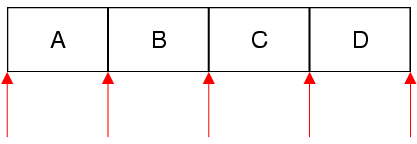
\includegraphics[width=0.5\textwidth]{javaiterators1}
	%\caption{model index}
\end{figure}


如果想查找特定值的所有实例,循环使用 findNext()。例如:

\begin{lstlisting}[language=C++]
QMutableHashIterator<int, QWidget *> i(hash);
while (i.findNext(widget)) {
    qDebug() << "Found widget " << widget << " under key "
             << i.key();
}
\end{lstlisting}

如果想在遍历哈希表时移除元素,使用 remove()。如果想修改元素的值,使用 setValue()。

例子:

\begin{lstlisting}[language=C++]
QMutableHashIterator<QString, QString> i(hash);
while (i.hasNext()) {
    i.next();
    if (i.key() == i.value())
        i.remove();
}
\end{lstlisting}

该示例移除所有键和值相等的键值对。

任何时候,对于给定哈希表,只能有一个活动的可修改迭代器。
而且,当迭代器处于活动状态时,
不可以(不通过迭代器)直接修改哈希表,因为这会使迭代器失效,并导致未定义行为。

\begin{seeAlso}
QHashIterator 和 QHash::iterator。
\end{seeAlso}

\section{成员函数文档}


bool QMutableHashIterator::findNext(const T \emph{\&value})

从当前迭代器位置开始向前查找值 \emph{value}。如果找到值为 \emph{value} 的键值对,返回 \hl{true};否则返回 \hl{false}。

调用该函数后,如果找到值 \emph{value},迭代器将被移动到匹配元素的后面;否则,迭代器将被移动到容器的末端。

const Key \&QMutableHashIterator::key() const

调用遍历函数(next(),findNext())后,该函数返回跳过的最后一个元素的键。

\begin{seeAlso}
value()。
\end{seeAlso}

T \&QMutableHashIterator::value()

这是一个重载函数。

返回调用遍历函数后跳过的最后一个元素值的非常量引用。

bool QMutableHashIterator::hasNext() const

如果该迭代器后面至少有一个元素,返回 \hl{true},即该迭代器不在容器的末端;否则返回 \hl{false}。

\begin{seeAlso}
next()。
\end{seeAlso}

void QMutableHashIterator::toBack()

将迭代器移动到容器的末端(最后一个元素之后)。

\begin{seeAlso}
toFront()。
\end{seeAlso}

void QMutableHashIterator::toFront()

将迭代器移动到容器的前端(第一个元素之前)。

\begin{seeAlso}
toBack() 和 next()。
\end{seeAlso}

QMutableHashIterator<Key, T> \&QMutableHashIterator::operator=(QHash<Key, T> \emph{\&container})

将迭代器关联到 \emph{container} 来遍历哈希表。
迭代器将被移动到哈希表的前端(第一个元素之前)。

\begin{seeAlso}
toFront() 和 toBack()。
\end{seeAlso}

QMutableHashIterator::QMutableHashIterator(QHash<Key, T> \emph{\&hash})

构造一个迭代器来遍历 \emph{hash}。迭代器将被移动到哈希表的前端(第一个元素之前)。

\begin{seeAlso}
operator=()。
\end{seeAlso}

QMutableHashIterator::Item QMutableHashIterator::next()

返回下一个元素并将迭代器向前移动一个位置。

对返回值调用 key() 获取元素的键,调用 value() 获取元素的值。

对位于容器末端的迭代器调用该函数将导致未定义结果。

\begin{seeAlso}
hasNext() 和 peekNext()。
\end{seeAlso}

QMutableHashIterator::Item QMutableHashIterator::peekNext() const

不移动迭代器而返回下一个元素。

对返回值调用 key() 获取元素的键,调用 value() 获取元素的值。

对位于容器末端的迭代器调用该函数将导致未定义结果。

\begin{seeAlso}
hasNext() 和 next()。
\end{seeAlso}

void QMutableHashIterator::remove()

移除使用遍历函数(next(),findNext())跳过的最后一个元素。

\begin{seeAlso}
setValue()。
\end{seeAlso}

void QMutableHashIterator::setValue(const T \emph{\&value})


用 \emph{value} 替换使用遍历函数跳过的最后一个元素的值。

遍历函数包括 next() 和 findNext()。

\begin{seeAlso}
key(),value() 和 remove()。
\end{seeAlso}

const T \&QMutableHashIterator::value() const

调用遍历函数(next(),findNext())后,该函数返回跳过的最后一个元素的值。

\begin{seeAlso}
key() 和 setValue()。
\end{seeAlso}
\chapter{QMutableMapIterator}

template <typename Key, typename T> class QMutableMapIterator

QMutableMapIterator 类为 QMap 和 QMultiMap 提供 Java 风格的非常量迭代器。更多内容...

\begin{tabular}{|r|l|}
	\hline
	属性 & 方法 \\
	\hline
    头文件  &	\hl{\#include <QMutableMapIterator>} \\
    \hline
    qmake: & QT += core    \\
	\hline
\end{tabular}

\begin{compactitem}[\arr]
\item 所有成员列表,包括继承的成员
\end{compactitem}

\section{公共成员函数}

\begin{longtable}[l]{|r|m{28em}|}   
    \hline
    返回类型 	& 函数 \\
    \hline
    & QMutableMapIterator(QMap<Key, T> \emph{\&map}) \\
    \hline
    QMutableMapIterator<Key, T> \& &	operator=(QMap<Key, T> \emph{\&container}) \\
    \hline
    bool 	&findNext(const T \emph{\&value}) \\ 
    \hline
    bool 	&findPrevious(const T \emph{\&value}) \\
    \hline
    bool &	hasNext() const \\
    \hline
    bool 	&hasPrevious() const \\ 
    \hline
    const Key \& 	&key() const \\ 
    \hline
    QMutableMapIterator::Item &	next() \\ 
    \hline
    QMutableMapIterator::Item &	peekNext() const  \\
    \hline 
    QMutableMapIterator::Item &	peekPrevious() const \\ 
    \hline
    QMutableMapIterator::Item &	previous() \\ 
    \hline
    void &	remove() \\ 
    \hline
    void &	setValue(const T \emph{\&value}) \\ 
    \hline
    void &	toBack() \\ 
    \hline
    void &	toFront() \\ 
    \hline
    const T \& &	value() const \\
    \hline 
    T \&  &	value() \\ 
    \hline
\end{longtable}


\section{详细描述}

QMap 同时提供 Java 风格迭代器 和 STL 风格迭代器。
Java 风格迭代器比 STL 风格迭代器更高级,更容易使用;同时也略微低效。

QMutableMapIterator<Key, T> 用来遍历并修改 QMap (或 QMultiMap) 。
如果不想修改 map(或者 QMap 是 const 的),可以使用更快速的 QMapIterator。

QMutableMapIterator 构造函数接受 QMap 作为参数。
构造后,迭代器位于 map 的最开始位置(第一个元素之前)。
下面的例子演示如何顺序遍历所有元素:

\begin{lstlisting}[language=C++]
QMap<int, QWidget *> map;
...
QMutableMapIterator<int, QWidget *> i(map);
while (i.hasNext()) {
    i.next();
    qDebug() << i.key() << ": " << i.value();
}
\end{lstlisting}

next() 函数返回 map 中的下一个元素并将迭代器前移。
key() 和 value() 函数返回跳过的最后一个元素的键和值。

与 STL 风格迭代器不同,Java 风格迭代器指向元素之间而不是直接指向元素。
第一次调用 next() 前移迭代器到第一个和第二个元素之间的位置,并返回第一个元素;
第二次调用 next() 前移迭代器到第二个和第三个元素之间的位置;以此类推。

%%%%%%%%

\begin{figure}[hbt!]  
	\centering
    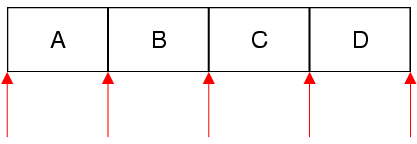
\includegraphics[width=0.5\textwidth]{javaiterators1}
	%\caption{model index}
\end{figure}


下面的例子演示如何反序遍历元素:

\begin{lstlisting}[language=C++]
QMutableMapIterator<int, QWidget *> i(map);
i.toBack();
while (i.hasPrevious()) {
    i.previous();
    qDebug() << i.key() << ": " << i.value();
}
\end{lstlisting}

如果想查找特定值的所有实例,循环使用 findNext() 或 findPrevious()。例如:

\begin{lstlisting}[language=C++]
QMutableMapIterator<int, QWidget *> i(map);
while (i.findNext(widget)) {
    qDebug() << "Found widget " << widget << " under key "
             << i.key();
}
\end{lstlisting}

如果想在遍历 map 时移除元素,使用 remove()。如果想修改元素的值,使用 setValue()。

例子:

\begin{lstlisting}[language=C++]
QMutableMapIterator<QString, QString> i(map);
while (i.hasNext()) {
    i.next();
    if (i.key() == i.value())
        i.remove();
}
\end{lstlisting}


该示例移除所有键和值相等的键值对。

任何时候,对于给定 map,只能有一个活动的可修改迭代器。
而且,当迭代器处于活动状态时,不可以直接修改 map,因为这会使迭代器失效,并导致未定义行为。

\begin{seeAlso}
QMapIterator 和 QMap::iterator。
\end{seeAlso}

\section{成员函数文档}

bool QMutableMapIterator::findPrevious(const T \emph{\&value})

从当前迭代器位置开始向后查找值 value。
如果找到值为 value 的键值对,返回 true;否则返回 false。

调用该函数后,如果找到值,迭代器将被移动到匹配元素的前面;
否则,迭代器将被移动到容器的前端。

\begin{seeAlso}
findNext()。
\end{seeAlso}

bool QMutableMapIterator::findNext(const T \emph{\&value})

从当前迭代器位置开始向前查找值 \emph{value}。
如果找到值为 \emph{value} 的键值对,返回 true;否则返回 false。

调用该函数后,如果找到值 \emph{value},迭代器将被移动到匹配元素的后面;否则,迭代器将被移动到容器的末端。

\begin{seeAlso}
findPrevious()。
\end{seeAlso}

const Key \&QMutableMapIterator::key() const

调用遍历函数(next(),previous(),findNext(),findPrevious())后,
该函数返回跳过的最后一个元素的键。

调用 next() 或 findNext() 后,key() 与 peekPrevious().key() 相同。
调用 previous() 或 findPrevious() 后,key() 与 peekNext().key() 相同。

\begin{seeAlso}
value()。
\end{seeAlso}

T \&QMutableMapIterator::value()

这是一个重载函数。

返回调用遍历函数后跳过的最后一个元素值的非常量引用。

QMutableMapIterator::Item QMutableMapIterator::peekPrevious() const

不移动迭代器而返回前一个元素。

对返回值调用 key() 获取元素的键,调用 value() 获取元素的值。

对位于容器前端的迭代器调用该函数将导致未定义结果。

\begin{seeAlso}
hasPrevious(),previous() 和 peekNext()。
\end{seeAlso}

QMutableMapIterator::Item QMutableMapIterator::previous()

返回前一个元素并将迭代器向后移动一个位置。

对返回值调用 key() 获取元素的键,调用 value() 获取元素的值。

对位于容器前端的迭代器调用该函数将导致未定义结果。

\begin{seeAlso}
hasPrevious(),peekPrevious() 和 next()。
\end{seeAlso}

bool QMutableMapIterator::hasPrevious() const

如果该迭代器前面至少有一个元素,返回 true,即该迭代器不在容器的前端;否则返回 false。

\begin{seeAlso}
hasNext() 和 previous()。
\end{seeAlso}

bool QMutableMapIterator::hasNext() const

如果该迭代器后面至少有一个元素,返回 true,即该迭代器不在容器的末端;否则返回 false。

\begin{seeAlso}
hasPrevious() 和 next()。
\end{seeAlso}

void QMutableMapIterator::toBack()

将迭代器移动到容器的末端(最后一个元素之后)。

\begin{seeAlso}
toFront() 和 previous()。
\end{seeAlso}

void QMutableMapIterator::toFront()

将迭代器移动到容器的前端(第一个元素之前)。

\begin{seeAlso}
toBack() 和 next()。
\end{seeAlso}

QMutableMapIterator<Key, T> \&QMutableMapIterator::operator=(QMap<Key, T> \&container)

将迭代器关联到 container 来遍历 map。
迭代器将被移动到 map 的前端(第一个元素之前)。

\begin{seeAlso}
toFront() 和 toBack()。
\end{seeAlso}

QMutableMapIterator::QMutableMapIterator(QMap<Key, T> \emph{\&map})

构造一个迭代器来遍历 \emph{map}。迭代器将被移动到 map 的前端(第一个元素之前)。

\begin{seeAlso}
operator=()。
\end{seeAlso}

QMutableMapIterator::Item QMutableMapIterator::next()

返回下一个元素并将迭代器向前移动一个位置。

对返回值调用 key() 获取元素的键,调用 value() 获取元素的值。

对位于容器末端的迭代器调用该函数将导致未定义结果。

\begin{seeAlso}
hasNext(),peekNext()和 previous()。
\end{seeAlso}

QMutableMapIterator::Item QMutableMapIterator::peekNext() const

不移动迭代器而返回下一个元素。

对返回值调用 key() 获取元素的键,调用 value() 获取元素的值。

对位于容器末端的迭代器调用该函数将导致未定义结果。

\begin{seeAlso}
hasNext(),next()和 peekPrevious()。
\end{seeAlso}

void QMutableMapIterator::remove()

移除使用遍历函数(next(),previous(),findNext(),findPrevious())跳过的最后一个元素。

\begin{seeAlso}
setValue()。
\end{seeAlso}

void QMutableMapIterator::setValue(const T \emph{\&value})

用 \emph{value} 替换使用遍历函数跳过的最后一个元素的值。

遍历函数包括 next(),previous(),findNext() 和 findPrevious()。

\begin{seeAlso}
key(),value() 和 remove()。
\end{seeAlso}

const T \&QMutableMapIterator::value() const

调用遍历函数(next(),previous(),findNext(),findPrevious())后,该函数返回跳过的最后一个元素的值。

调用 next() 或 findNext() 后,value() 与 peekPrevious().value() 相同。
调用 previous() 或 findPrevious() 后,value() 与 peekNext().value() 相同。

\begin{seeAlso}
key() 和 setValue()。
\end{seeAlso}
\chapter{QMutex}

QMutex类提供线程间的访问序列化。\href{https://github.com/QtDocumentCN/QtDocumentCN/blob/master/Src/M/QMutex/QMutex.md#%E8%AF%A6%E7%BB%86%E6%8F%8F%E8%BF%B0}{更多...}

\begin{tabular}{|r|l|}
	\hline
	属性 & 内容 \\
	\hline
    头文件  &	\hl{\#include<QMutex>} \\
    \hline
    qmake: & QT += core    \\
	\hline
    子类 	& QRecursiveMutex \\ 
    \hline
\end{tabular}

\begin{compactitem}
\item 此类中所有函数都是线程安全的。
\end{compactitem}

\section{公共成员类型}


\begin{tabular}{|r|m{28em}|}   
\hline
类型 	& 名称 \\ 
\hline
enmu 	& RecursionMode \{ Recursive, NonRecursive \} \\ 
\hline
\end{tabular}

\section{公共成员函数}

\begin{longtable}{|r|m{28em}|}   
    \hline
    返回类型 	& 函数 \\
    \hline
   & QMutex(QMutex::RecursionMode mode) \\
    \hline
	&QMutex() \\ 
    \hline
	&$\sim$QMutex() \\ 
    \hline
bool &	isRecursive() const \\ 
\hline
void &	lock() \\ 
\hline
bool 	&tryLock(int timeout = 0) \\ 
\hline
bool 	&try\_lock() \\ 
\hline
bool &	try\_lock\_for(std::chrono::duration<Rep, Period> \emph{duration}) \\ 
\hline
bool 	&try\_lock\_until(std::chrono::time\_point<Clock, Duration> \emph{timePoint}) \\ 
\hline
void &	unlock() \\ 
    \hline 
\end{longtable}


\section{详细描述}

QMutex的目的是保护对象、数据结构或代码段,以便一次只有一个线程可以访问它们(这类似于 Java synchronized 关键字)。
最好通过 QMutexLocker 来使用互斥量,这样可以很方便确保成对执行锁和解锁。
例如,假设有一个方法将消息打印到两行上:

\begin{cppcode}
int number = 6;

void method1()
{
    number *= 5;
    number /= 4;
}

void method2()
{
    number *= 3;
    number /= 2;
}
\end{cppcode}

如果连续调用这两个方法,将发生以下情况:

\begin{cppcode}
// method1()
number *= 5;        // number 30
number /= 4;        // number  7

// method2()
number *= 3;        // number 21
number /= 2;        // number 10
\end{cppcode}

如果两个线程同时调用这两个方法,则可能会产生以下结果:

\begin{cppcode}
// 线程 1 调用 method1()
number *= 5;        // number 30

// 线程 2 调用 method2().
//
// 很可能线程 1 已被操作系统置于等待队列
// 操作系统运行线程 2
number *= 3;        // number 90
number /= 2;        // number 45

// 线程 1 执行完毕
number /= 4;        // number 是 11,而不是 10
\end{cppcode}

如果我们添加一个互斥量,我们就能得到我们想要的结果:

\begin{cppcode}
QMutex mutex;
int number = 6;

void method1()
{
    mutex.lock();
    number *= 5;
    number /= 4;
    mutex.unlock();
}

void method2()
{
    mutex.lock();
    number *= 3;
    number /= 2;
    mutex.unlock();
}
\end{cppcode}

在任何给定的时间只有一个线程可以修改 number,并正确执行。
虽然这只是一个微不足道的例子,但也适用于其他需要有序执行的地方。

当你在一个线程中调用 lock() 时,在同一位置尝试调用 lock() 的其他线程将阻塞,
直到获得锁的线程调用 unlock()。
替代 lock() 的非阻塞方法是 tryLock()。

QMutex被优化为在非争用情况 ( the non-contended )下速度更快。
如果互斥体上没有争用,非递归QMutex将不会分配内存。
它的构造和销毁几乎没有任何开销,
这意味着将互斥体作为类的一部分是很好的做法。

\begin{seeAlso}
QRecursiveMutex,QMutexLocker,QReadWriteLock,QSemaphore 和 QWaitCondition。
\end{seeAlso}

\section{成员类型文档}

enum QMutex::RecursionMode

\begin{tabular}{|c|c|m{20em}|}
\hline
常量 	&值& 	描述 \\ 
\hline
QMutex::Recursive &	1 	&在这种模式下,一个线程可以多次锁定同一个互斥量,并且在调用相同数量的 unlock() 之前,互斥体不会被解锁。对于这种情况,您应该使用 QRecursiveMutex。 \\
\hline
QMutex::NonRecursive &	0 	&在这种模式下,一个线程只能锁定一次。\\
\hline
\end{tabular}

\begin{seeAlso}
QMutex(),QRecursiveMutex。
\end{seeAlso}

\section{成员函数文档}

QMutex::QMutex(QMutex::RecursionMode \emph{mode})

构造一个互斥量,初始状态为未上锁。

如果 mode 是 QMutex::Recursive,则线程可以多次锁定同一个互斥量,
并且在调用相同数量的 unlock() 之前,互斥量不会被解锁。
否则,线程只能锁定互斥量一次。默认值为 QMutex::NonRecursive。

\begin{seeAlso}
lock(),unlock()。
\end{seeAlso}

QMutex::QMutex()

构造一个互斥量,初始状态为未上锁。

QMutex::$\sim$QMutex()

析构。

\begin{warning}
销毁锁定的互斥量可能会导致未定义的行为。
\end{warning}

bool QMutex::isRecursive() const

如果互斥量是递归的,则返回 true。

在 Qt 5.7 引入该函数。

void QMutex::lock()

锁定互斥量。如果另一个线程锁定了该互斥量,
那么这个调用将被阻塞,直到锁定线程将其解锁为止。

如果该互斥量是递归互斥量,则允许在同一线程的同一互斥体上多次调用此函数。
如果这个互斥量是非递归互斥量,则当该互斥量递归锁定时,这个函数将死锁。

\begin{seeAlso}
unlock()。
\end{seeAlso}

bool QMutex::tryLock(int \emph{timeout} = 0)

尝试锁定互斥量。如果获得了锁,此函数返回 true;否则返回 false。
如果另一个线程锁定了互斥量,则此函数最多将等待 timeout 毫秒,以尝试获取。

\begin{notice}
传递一个负数给 timeout 相当于调用 lock()。即,如果 timeout 为负数,
这个函数将一直待,直到互斥量被锁定为止。
\end{notice}

如果获得了锁,则必须使用 unlock() 解锁,另一个线程才能成功锁定。

如果该互斥量是递归互斥量,则允许在同一线程的同一互斥量上多次调用此函数。
如果此互斥量是非递归互斥量,则当尝试递归锁定互斥量时,此函数将始终返回 false。

\begin{seeAlso}
lock(),unlock()。
\end{seeAlso}

bool QMutex::try\_lock()

尝试锁定互斥量。如果获得了锁,此函数返回 true;否则返回 false。

提供此函数是为了与可锁定的标准库概念兼容。它相当于 tryLock()。

在 Qt 5.8 引入该函数。

template <typename Rep, typename Period> bool QMutex::try\_lock\_for(std::chrono::duration<Rep, Period> duration)

尝试锁定互斥量。如果获得了锁,此函数返回 true;否则返回 false。
如果另一个线程锁定了互斥量,则此函数最多将等待 duration 这么长时间,
以尝试获取。

\begin{notice}
传递一个负数给 duration 相当于调用 try\_lock()。
\end{notice}

此行为与 tryLock() 不同。

如果获得了锁,则必须使用 unlock() 解锁,另一个线程才能成功锁定。

如果该互斥量是递归互斥量,则允许在同一线程的同一互斥量上多次调用此函数。
如果此互斥量是非递归互斥量,则当尝试递归锁定互斥量时,此函数将始终返回 false。

在 Qt 5.8 引入该函数。

\begin{seeAlso}
lock(),unlock()。
\end{seeAlso}

template <typename Clock, typename Duration> bool QMutex::try\_lock\_until(std::chrono::time\_point<Clock, Duration> \emph{timePoint})

尝试锁定互斥量。如果获得了锁,此函数返回 true;否则返回 false。
如果另一个线程锁定了互斥量,则此函数最多将等待 timePoint 这么长时间,
以尝试获取。

\begin{notice}
传递一个负数给 timePoint 相当于调用 try\_lock()。
\end{notice}

此行为与 tryLock() 不同。

如果获得了锁,则必须使用 unlock() 解锁,另一个线程才能成功锁定。

如果该互斥量是递归互斥量,则允许在同一线程的同一互斥量上多次调用此函数。
如果此互斥量是非递归互斥量,则当尝试递归锁定互斥量时,此函数将始终返回 false。

在 Qt 5.8 引入该函数。

\begin{seeAlso}
lock(),unlock()。
\end{seeAlso}

void QMutex::unlock()

解锁互斥量。试图在不同线程中解锁互斥量会导致错误。
解锁未锁定的互斥量会导致未定义的行为。

\begin{seeAlso}
lock()。
\end{seeAlso}


\chapter{QMutexLocker}

QMutexLocker 是一个工具类,它能非常方便地将互斥量锁定以及解锁。更多内容...

\begin{tabular}{|r|l|}
	\hline
	属性 & 内容 \\
	\hline
    头文件  &	\hl{\#include<QMutexLocker>} \\
    \hline
    qmake: & QT += core    \\
	\hline
\end{tabular}

\begin{compactitem}[\arr]
\item 此类中所有函数都是线程安全的。
\end{compactitem}

\section{公共成员函数}

\begin{tabular}{|r|l|}   
    \hline
    返回类型 	& 函数 \\
    \hline
    & QMutexLocker(QRecursiceMutex \emph{*mutex}) \\ 
    \hline
	&QMutexLocker(QMutex \emph{*mutex}) \\ 
    \hline
	& $\sim$QmutexLocker() \\ 
\hline
QMutex * &	mutex() const \\
\hline
void 	& relock()\\
\hline
void 	& unlock() \\ 
    \hline 
\end{tabular}


\section{详细描述}

在复杂的函数、语句或异常处理代码中锁定和解锁 QMutex 很容易出错,而且很难调试。
QMutexLocker 可用于此类情况,
以确保互斥量的状态始终定义良好。

QMutexLocker 应该在需要锁定 QMutex 的函数中创建。在创建 QMutexLocker 时互斥量被锁定。
您可以使用 unlock() 和 relock() 解锁和重新锁定互斥体。如果锁定,则当 QMutexLocker 被销毁时,互斥量将被解锁。

例如,此复杂函数在进入函数时锁定 QMutex,并在所有出口点解锁互斥量:很方便确保成对执行锁和解锁。
例如,假设有一个方法将消息打印到两行上:

\begin{lstlisting}[language=C++]
    int complexFunction(int flag)
    {
        mutex.lock();

        int retVal = 0;

        switch (flag) {
        case 0:
        case 1:
            retVal = moreComplexFunction(flag);
            break;
        case 2:
            {
                int status = anotherFunction();
                if (status < 0) {
                    mutex.unlock();
                    return -2;
                }
                retVal = status + flag;
            }
            break;
        default:
            if (flag > 10) {
                mutex.unlock();
                return -1;
            }
            break;
        }

        mutex.unlock();
        return retVal;
    }
\end{lstlisting}

该示例在开发过程中会变得更加复杂,也更加容易出错。 
使用 QMutexLocker 可大大简化代码,且可读性更好:

\begin{lstlisting}[language=C++]
    int complexFunction(int flag)
    {
        QMutexLocker locker(&mutex);

        int retVal = 0;

        switch (flag) {
        case 0:
        case 1:
            return moreComplexFunction(flag);
        case 2:
            {
                int status = anotherFunction();
                if (status < 0)
                    return -2;
                retVal = status + flag;
            }
            break;
        default:
            if (flag > 10)
                return -1;
            break;
        }

        return retVal;
    }
\end{lstlisting}

现在,当 QMutexLocker 对象被销毁时(当函数返回时,因为 locker 是一个栈变量),互斥量将始终被解锁。
同样的原则也适用于抛出和捕获异常的代码。
在将异常传递给调用函数之前,如果函数未在锁定互斥量的函数中捕获到异常,则无法解锁互斥体。

(译者注:在进入被调函数后,被调函数锁定互斥量(使用QMutex::lock()),
在执行过程中发生异常,异常被调用函数获取,被调函数就没有正确执行解锁。)

QMutexLocker 还提供一个 mutex() 成员函数,该函数返回QMutexLocker 正在其上操作的互斥体。
这对于需要访问互斥体的代码非常有用,例如 QWaitCondition::wait()。

例如:

\begin{lstlisting}[language=C++]
    class SignalWaiter
    {
    private:
        QMutexLocker locker;

    public:
        SignalWaiter(QMutex *mutex)
            : locker(mutex)
        {
        }

        void waitForSignal()
        {
            ...
            while (!signalled)
                waitCondition.wait(locker.mutex());
            ...
        }
    };
\end{lstlisting}

\begin{seeAlso}
ReadLockr,QWriteLocker,QMutex。
\end{seeAlso}

%%%%%%%%%%%%%%%%

\section{成员函数文档}

QMutexLocker::QMutexLocker(QRecursiveMutex \emph{*mutex})

构造一个 QMutexLocker 并锁定互斥量。
当 QMutexLocker 被销毁时,互斥量将被解锁(unlock())。
如果 mutex 为空,那么 QMutexLocker 不执行任何操作。

在 Qt5.14 中引入该函数。

\begin{seeAlso}
QMutex::lock()
\end{seeAlso}

QMutexLocker::QMutexLocker(QMutex \emph{*mutex})

构造一个 并锁定互斥量。当 QMutexLocker 被销毁时,互斥量将被解锁。
如果 mutex 为空,那么 QMutexLocker 不执行任何操作。

\begin{seeAlso}
QMutex::lock()
\end{seeAlso}

QMutexLocker::$\sim$QMutexLocker()

销毁 QMutexLocker 并解除锁定构造函数中锁定的互斥量。

\begin{seeAlso}
QMutex::unlock()
\end{seeAlso}

QMutex *QMutexLocker::mutex() const

返回 QMutexLocker 正在操作的互斥量。

void QMutexLocker::relock()

重新锁定,未上锁的互斥量。

\begin{seeAlso}
unlock()
\end{seeAlso}

void QMutexLocker::unlock()

解锁这个互斥量。
您可以使用 relock() 再次锁定它。销毁时不需要锁定。

\begin{seeAlso}
relock()
\end{seeAlso}
\chapter{元对象系统}

Qt 的元对象系统提供了对象间通信的信号槽机制、运行时类型信息,以及动态属性系统。

元对象系统基于以下三者:

\begin{compactenum}
\item QObject 类,提供了便于利用元对象系统的基类;
\item Q\_OBJECT 宏,放置于类声明的私有域,用于激活元对象系统特性,例如动态属性和信号槽;
\item 元对象编译器 (moc),为每个 QObject 的子类提供实现元对象特性的代码生成。
\end{compactenum}

moc 工具读取 C++ 源文件,若在其中找到包含 Q\_OBJECT 宏的类声明,
则会创建另一个 C++ 源文件,并在其中填充用于实现元对象得的代码。
该生成的源文件需要通过 \#include' 包含至对应类的源文件,
或者更常见的是将其加入编译列表,并于对应类的实现一同链接。

\begin{compactitem}
\item QObject::metaObject() 返回该类对应的 元对象。
\item QMetaObject::className() 在运行时以字符串形式返回该类的类名,并且不需要依赖 C++ 编译器的运行时类型信息(RTTI)支持;
\item QObject::inherits() 函数返回该对象所属类型,是否派生自 QObject 继承树中的指定类型;
\item QObject::tr() 和 QObject::trUtf8() 为 国际化 支持提供字符串翻译;
\item QObject::setProperty() 和 QObject::property() 用于通过属性名称,动态设置和读取属性值;
\item QMetaObject::newInstance() 构建指定类的新实例。
\end{compactitem}

我们还可以对 QObject 进行 qobject\_cast() 操作,
该函数与标准 C++ 的 dynamic\_cast() 表现类似,
但优点时不需要 RTTI 支持,并且可以跨越动态库边界运作。
它会尝试将输入指针转换为尖括号中的指针类型,
若类型正确则返回非空指针(在运行时作出判断),
若对象类型不兼容则返回 nullptr。

例如,假设 MyWidget 继承自 QWidget 类,并声明了 Q\_OBJECT 宏:

\begin{cppcode}
QObject *obj = new MyWidget;
\end{cppcode}

QObject * 类型的变量 obj 实际指向一个 MyWidget 对象,于是我们可以进行如下转换:

\begin{cppcode}
QWidget *widget = qobject_cast<QWidget *>(obj);
\end{cppcode}

从 QObject 到 QWidget 的转换成功进行,
因为该对象实际是 QWidget 的子类 MyWidget。
由于我们知道 obj 是 MyWidget 类型,
我们可以将其转换为 MyWidget *:

\begin{cppcode}
MyWidget *myWidget = qobject_cast<MyWidget *>(obj);
\end{cppcode}

转换至 MyWidget 的操作可以成功进行,因为 qobject\_cast() 并不会将 Qt 内置类型和自定义类型区别对待。
(译者注:Qt 是在运行时通过读取元对象信息进行动态转换,开发者可通过 Q\_OBJECT 宏让自定义类型支持被 qobject\_cast() 进行转换)

\begin{cppcode}
QLabel *label = qobject_cast<QLabel *>(obj);
// label is 0
\end{cppcode}

另一个例子,转换为 QLabel 的操作失败了,该指针会被置零。但此机制也让运行时基于转换结果来区别处理不同类型成为可能:

\begin{cppcode}
if (QLabel *label = qobject_cast<QLabel *>(obj)) {
    label->setText(tr("Ping"));
} else if (QPushButton *button = qobject_cast<QPushButton *>(obj)) {
    button->setText(tr("Pong!"));
}
\end{cppcode}

虽然可以使用 QObject 作为基类,
但不定义 Q\_OBJECT 宏,也不生成元对象代码,
但这也意味着信号槽以及本文提到所有的其它机制无法使用。
从元对象系统的视角来看,没有元对象代码的 QObject 的子类
(译者注:即未使用 Q\_OBJECT 宏)等价于它最近的一个包含元对象代码的父类,
这也意味着,例如,QMetaObject::className() 不会返回该类的类名,而是会返回父类的类名。

因此,我们强烈建议在所有 QObject 的子类中都使用 Q\_OBJECT 宏,
无论它们是否用到了信号槽和动态属性。

\begin{seeAlso}
QMetaObject,Qt 的属性系统 以及 信号与槽。
\end{seeAlso}
\chapter{为何 Qt 使用 Moc 实现信号槽?}

模板是 C++ 的内建机制,可以允许编译器基于传递的参数类型,在编译期生成代码。
因此,框架编写者很喜欢使用模板,而我们也的确在 Qt 的许多地方使用了高阶的模板特性。然而,模板有限制的:
有的东西可以用模板很轻易地表达,但同样也会有几乎无法用模板表达的东西。
一个通用的向量容器类很容易用模板表达,即使它在针对指针类型时使用到了偏特化特性;
然而一个基于 XML 字符串的内容描述来构建用户界面的函数,就无法用模板来表达。
并且,在它俩之间还有一块灰色区域。
强行使用模板来实现功能,会付出代码体积、可读性、可移植性、可用性、
可扩展性、健壮性乃至最根本的设计美感上的代价。
C++ 的模板和 C 的宏都可以用于扩展语法,来实现不可思议又难以置信的奇思妙想,
但这只代表这些想法是可行的,
而未必意味着这么做是正确的设计思路。很不幸,编写代码,并不是用来写进书籍(译者注:即阳春白雪般的纸上谈兵),
而是在真实世界的操作系统中,被真实世界的编译器所编译。

这就是为什么 Qt 使用 moc 的原因:

\section{语法很重要}

语法并不只是糖:用于描述我们的算法的语法,会显著地影响我们的代码的可读性和可维护性。
Qt 的信号槽语法被证明是非常成功的实践,它的语法非常直观,易于使用也易于阅读。
学习 Qt 时,这种语法可以帮助人们更好地理解和使用信号槽这个概念——尽管它本质上是很高阶的通用抽象。
这令开发者们在刚踏入门槛时,就能做出正确的设计,甚至都不需要去思考何为设计模式。

\section{代码生成是好东西}

Qt 的 moc(Meta Object Compiler,元对象编译器) 提供了一种简洁的方式,
来超越目标语言本身的桎梏。它通过生成额外的 C++ 代码来达成目标,而这些代码可以被任何标准的 C++ 编译器所编译。
moc 会阅读 C++ 源码文件,如果找到任何类声明中包含了 Q\_OBJECT 宏,
就会生成另一个 C++ 源码文件,在其中填充这些类的元对象相关的代码。
moc 生成的 C++ 源码文件必须与对应类的实现文件共同编译和链接(也可以被\#include包含到对应类的源文件中)。
但通常来说,moc 并不会被手动调用,而是被编译系统自动调用,因此不需要开发者做额外工作。

moc 并不是 Qt 使用的唯一一个代码生成器。
另一个典型范例则是 uic(User Interface Compiler,用户界面编译器),
它接受 XML 格式的用户界面描述,来生成 C++ 代码并初始化界面。在 Qt 之外,
代码生成器同样也被广泛应用,例如 rpc 和 idl,
可以支撑应用程序或对象跨越进程甚至跨机器进行通信。又比如,
各种各样的词法分析工具,如大名鼎鼎的 lex 和 yacc,
它们将语法规范作为输入,来生成可以实现这些规范的状态机代码。
代码生成器的其它替代品有改造编译器、专有语言或者可视化编程工具——后者提供单向的对话框/向导,
用于在设计阶段而非编译阶段生成各种晦涩的代码。相比于将我们的客户绑定在专用的 C++ 编译器上,
或者绑定到特定的集成开发环境(IDE)中,我们允许他们使用任何他们喜欢的工具。
相较于强迫开发者将生成的代码添加到代码库中,
我们更鼓励他们将我们的工具添加到他们的构建系统中:更加干净、更加安全、更具有 UNIX 精神。

\begin{quote}
译者注:UNIX 精神指的是用小型单一工具组合完成任务,而非庞大的、无所不能的复杂工具。
\end{quote}


\section{用户界面是动态的}

C++ 是一门标准化的、强大的、经过精心设计的通用型语言,它是唯一一门被应用于如此广泛的软件开发领域的语言,囊括了所有种类的应用程序,
包括完整的操作系统、数据库服务器、高级图形应用乃至于通用桌面应用。C++ 成功的关键之一,便是在提供可伸缩的语言特性的同时,聚焦于最大化性能和最小化内存占用,同时还保持了对 ANSI C 的兼容性。
除此之外,C++ 也有一些缺点。例如在面对基于组件的用户界面开发时,C++ 的静态对象模型相较于 Objective-C 的动态消息机制便是很显著的劣势。
对于高级数据库服务器或者操作系统而言的优秀特性,却并非用户界面前端设计的正确选择。
拥有了 moc 后,我们可以将这个劣势转化为优势,为满足安全又高效的用户界面开发提供了充足的灵活性。
我们的成果已经超越了通过模板能够做到的任何事情。例如,我们可以拥有对象属性,
还可以重载信号槽,这在一门把重载作为关键特性的语言中,会令开发者感到无比自然。我们的信号机制不会让对象大小增加任何一个字节,这意味着我们在添加新的信号的同时不会破坏二进制兼容性。
另一个好处是我们可以在运行时检索一个对象的信号和槽。我们可以通过名称(译者注:字符串)来做到类型安全地建立连接,
而并不需要知道我们连接的对象使用的具体类型(译者注:包括对象类型和参数类型),这对于基于模板的解决方案来说是不可能的。这种运行时的自省机制为我们开启了新的可能,例如,可以通过 Qt Designer 的 XML 界面文件来生成图形界面,并完成信号槽的连接。

\section{调用性能并不代表一切}

Qt 的信号槽实现并不能和基于模板的解决方案一样快。
尽管发射一个信号大约只有四次常规模板函数的调用开销,
整个信号槽执行的过程也只被 Qt 尽量压缩到10倍函数调用开销。
这并不令人意外,因为 Qt 的机制包括了通用的序列化、自省、不同线程间的队列执行以及极致的脚本化。
它并不需要激进的内联和代码展开,但却提供了远超于这些代价的运行时安全性。
Qt 的信号分发机制是安全的,而那些速度更快的基于模板的系统则不是。
即使在发送一个信号至多个不同的接收者的过程中,
您依然可以安全地删除这些接收者,而不会引发程序崩溃。
如果没有这份安全性,您的程序可能会偶发性地崩溃,
并伴随一个痛苦的调试过程,来修复错误地对已经被释放掉的内存进行的读写操作。


\begin{quote}
译者注:

本段翻译有待商榷,其中一句

Qt 的信号分发机制是安全的,而那些速度更快的基于模板的系统则不是。

对应的原文是

Qt's iterators are safe while those of faster template-based systems are not.

从字面理解,该句是指 Qt 容器的迭代器。然而结合上下文,该句应该也是用于描述信号槽机制的安全性,所以此处理解为信号分发过程中,遍历分发目标的安全性,即 iteration 操作。

然而,从 Qt 容器安全性上理解也未尝不可。虽然迭代器算法是和容器数据结构强相关,对于相同类型的容器,Qt 迭代器与 STL 迭代器算法本质上并无区别,但 STL 容器是由标准库实现,而不同平台的标准库实现是针对该平台高度特化的,这导致了即使是很规范的 C++ 代码,移植到不同平台后依然可能因为平台差异(如大小端、位宽、对齐)产生 bug——而这不会出现在 Qt 中,因为 Qt 的设计是宁可舍弃平台特化的性能,也要保证兼容性。
\end{quote}


尽管如此,难道就不能用基于模板的方案来提升使用信号槽的应用的性能吗?
尽管 Qt 的确在信号槽调用中增加了一点点额外开销,这个开销对于槽的整个执行过程只占了很小的比例。
只要在槽里做了任何有效的操作,例如一些简单的字符串处理,那么调用时的额外开销就可以忽略不计了。
Qt 的系统已经经过充分优化,以至于任何需要new/delete的操作(例如字符串操作或向模板容器中插入/删除对象),
都比发射一次信号有更可观的开销。

例外:如果您在某个性能敏感任务的内部循环中使用了信号槽,并且确认它成为性能瓶颈,
那么可以考虑将其更换为监听者模式(译者注:更通用的称呼是发布-订阅或生产者-消费者)。
在这类场景中,您可能只需要一对一的连接方式。例如,如果有一个对象从网络中下载数据,
使用信号来标识需要的数据已经接收到,会是明智的设计;
但如果需要将每个字节逐一发送至一个消费者,就应该使用监听者模式而非信号槽。

\section{不受限制}

因为有 moc 来实现信号槽,我们可以添加更多模板所不能做到的东西。
其中便有带作用域的翻译器,可以通过生成的 tr() 函数使用;
还有一个先进的属性系统,具备运行时的自省和类型信息。
属性系统具有一个显著的优点:如 Qt Disigner 这类强大而且通用的可视化界面设计工具,
如果没有强大的支持反射的属性系统支撑的话,
会极其难以编写(如果的确能够编写出来的话)。
但不止于此,我们还提供了一个 qobject\_cast<T>() 动态转换机制,
并且不需要依赖系统的 RTTI 特性,也不需要承担 RTTI 所受的限制,
我们使用它来从动态加载的组件中安全地获取接口。
另一个应用领域是动态的元对象,例如,我们可以获取一个 ActiveX 组件,
并且在运行时为其生成对应的元对象;或者,我们也可以通过导出元对象的形式,将 Qt 组件导出为 ActiveX 组件。使用模板无法做到其中任意一个。

C++ 结合 moc 为我们提供了类似于 Objective-C 或者 JRE(Java Runtime Environment, 
Java 运行时环境) 的灵活性,
但同时依然保留了 C++ 独有的性能与扩展性优势。这让我们如今使用的 Qt 成为了一个灵活而方便的工具。
\chapter{QReadLocker}

QReadLocker 是工具类,它简化了对读写锁,读访问的的锁定和解锁。\href{https://gitee.com/wcc210/QtDocumentCN/blob/master/Src/R/QReadLocker/QReadLocker.md#%E8%AF%A6%E7%BB%86%E6%8F%8F%E8%BF%B0}{更多...}

\begin{tabular}{|l|l|}
\hline
属性 &	方法\\
\hline
头文件:& 	\#include <QReadLocker>\\
\hline
qmake:& 	QT += core\\
\hline
\end{tabular}

\begin{notice}
此类中全部函数可重入。
\end{notice}

\section{公共成员函数}

\begin{tabular}{|l|m{23em}|}
\hline
类型 &	名称\\
\hline
 &	QReadLocker(QReadWrtiteLock \emph{*lock}) \\
\hline
 &	$\sim$QReadLocker() \\ 
\hline
QReadWriteLock * &	readWriteLock() const \\ 
\hline
void &	relock() \\ 
\hline
void &	unlock() \\
\hline
\end{tabular}

\section{详细描述}

QReadLocker(和 QWriteLocker)的目的是简化 QReadWriteLock 的锁定和解锁。锁定和解锁语句、异常处理代码是很容易出错的,而且很难调试。QReadLocker 可以确保在此类情况下,锁的状态始终定义良好。

下面是一个使用 QReadLocker 锁定和解锁读写锁的示例:

\begin{lstlisting}[language=C++]
QReadWriteLock lock;

QByteArray readData()
{
    QReadLocker locker(&lock);
    ...
    return data;
}
\end{lstlisting}

等价于以下代码:

\begin{lstlisting}[language=C++]
ReadWriteLock lock;

QByteArray readData()
{
    lock.lockForRead();
    ...
    lock.unlock();
    return data;
}
\end{lstlisting}

QMutexLocker 文档展示了使用locker对象来大大简化编程的示例。

\begin{notice}[另请参阅]
QWriteLocker、QReadWriteLock。
\end{notice}

\section{成员函数文档}

ReadLocker::QReadLocker(QReadWriteLock \emph{*lock})

构造一个 QReadLocker 并锁定用于读取的锁。当 QReadLocker 被销毁时,锁将被解锁。如果 lock == nullptr,则 QReadLocker 不执行任何操作。


\begin{notice}[另请参阅]
QReadWriteLock::lockForRead()。
\end{notice}

QReadLocker::$\sim$QReadLocker()

销毁 QReadLocker 并解锁传递给构造函数的锁。

\begin{notice}[另请参阅]
QReadWriteLock::unlock()。
\end{notice}

QReadWriteLock *QReadLocker::readWriteLock() const

返回传递给构造函数的读写锁的指针。

void QReadLocker::relock()

重新锁定。

\begin{notice}[另请参阅]
unlock()。
\end{notice}


void QReadLocker::unlock()

解锁。

\begin{notice}[另请参阅]
QReadWriteLock::unlock()。
\end{notice}
\chapter{QReadWriteLock}

QReadWriteLock 类提供读写锁定。更多...

\begin{tabular}{|l|l|}
\hline
属性 &	方法\\
\hline
头文件:& 	\#include <QReadWriteLock>\\
\hline
qmake:& 	QT += core\\
\hline
\end{tabular}

\begin{notice}
此类中所有函数都是线程安全的。
\end{notice}

\section{公共成员类型}

\begin{tabular}{|l|l|}
\hline
类型 &	名称\\
\hline
enmu 	& RecursionMode \{ Recursive, NonRecursive\}\\
\hline
\end{tabular}


\section{公共成员函数}

\begin{tabular}{|l|l|}
\hline
返回类型 &	函数 \\ 
\hline
& QReadWriteLock(QReadWriteLock::RecursionMode \emph{recursionMode} = NonRecursive) \\
\hline
& $\sim$QReadWriteLock() \\ 
void &	lockForRead() \\ 
\hline
void &	lockForeWrite() \\ 
\hline
bool &	tryLockForRead()\\ 
\hline
bool &	tryLockForRead(int \emph{timeout}) \\ 
\hline
bool &	trylockForWrite() \\ 
\hline
bool &	trylockForWrite(int \emph{timeout}) \\ 
\hline
void &	unlock() \\ 
\hline
\end{tabular}

\section{详细描述}

读写锁是一种用于保护读写资源的同步工具。
如果希望允许多个线程同时进行只读访问,那么这种类型的锁很有用,但是只要一个线程想写入资源,那么它就必须阻止所有其他线程,直到写入完成。
  
在许多情况下,QReadWriteLock 是 QMutex 强有力的竞争对手。
QReadWriteLock 在多并发读,少量写的情况下,有较好的执行效果。

例如:

\begin{lstlisting}[language=C++]
QReadWriteLock lock;

void ReaderThread::run()
{
    ...
    lock.lockForRead();
    read_file();
    lock.unlock();
    ...
}
    
void WriterThread::run()
{
    ...
    lock.lockForWrite();
    write_file();
    lock.unlock();
    ...
}
\end{lstlisting}

为了确保写者永远不会被读者阻塞,如果有写者被阻塞,则读者将无法获取锁,
即使该锁当前正被其他读者访问。另外,如果一个写者正在写,而另一个写者想进入,则该写者将优先于其他可能正在等待的读者。

与 QMutex 类似,当使用 QReadWriteLock::Recursive 作为 QReadWriteLock::RecursiveMode 参数构造时,QReadWriteLock 可以被同一线程递归锁定。在这种情况下,
unlock() 的调用次数必须与 lockForWrite() 或 lockForRead() 的调用次数相同。
请注意,当尝试递归锁定时,不能更改锁类型,也就是说,在已经为写入而锁定的线程中,不可能为读取而锁定(反之亦然)。

\begin{seeAlso}
QReadLock、QWriteLock、QMutex、QSemaphore。
\end{seeAlso}

\section{成员类型文档}

enum QReadWriteLock::RecursionMode

\begin{tabular}{|l|l|l|}
\hline
常量 &	值  &	描述 \\ 
\hline
QReadWriteLock::Recursive  &	1  &	  在这种模式下,线程可以多次锁定同一个 QReadWriteLock。QReadWriteLock 在执行相应数量的 unlock() 调用之前不会解锁。 \\ 
\hline
QReadWriteLock::NonRecursive &	0 	&  在这种模式下,线程只能锁定 QReadWriteLock 一次。 \\ 
\hline
\end{tabular}

\begin{seeAlso}
QReadWriteLock()。
\end{seeAlso}

\section{成员函数文档}

QReadWriteLock::QReadWriteLock(QReadWriteLock::RecursionMode recursionMode = NonRecursive)

构造一个 \hl{recursionMode} 模式的 \hl{QReadWriteLock}。
默认 NonRecursive。

在 Qt 4.4 引入该函数。


\begin{seeAlso}
lockForRead()、lockForWrite()、RecursiveMode。
\end{seeAlso} 

QReadWriteLock::$\sim$QReadWriteLock()

解锁,并析构。

\begin{notice}[警告]
销毁正在使用的读写锁可能会导致未定义的行为。
\end{notice} 

void QReadWriteLock::lockForRead()

读锁定。如果另一个线程正写锁定,则此函数将阻塞当前线程。
如果线程已写锁定,则不可读锁定。

\begin{seeAlso}
unlock()、lockForWrite()、tryLockForWrite()。
\end{seeAlso} 

void QReadWriteLock::lockForWrite()

写锁定。如果另一个线程(包括当前线程)为读或写而锁定(除非锁是使用 QReadWriteLock::Recursive 模式创建的),则此函数将阻塞当前线程。   如果线程已读锁定,则不可写锁定。

\begin{seeAlso}
unlock()、lockForWrite()、tryLockForWrite()。
\end{seeAlso} 

bool QReadWriteLock::tryLockForRead()

尝试读锁定。如果获得了锁,此函数将返回 true,否则将返回 false,而不是等待锁变为可用,即不阻塞。
如果另一个线程已写锁定,则读锁定尝试将失败。
如果获得了锁,请务必使用 unlock() 解锁,然后另一个线程才能成功地将其写锁定。
如果线程已写锁定,则不可读锁定。

\begin{seeAlso}
unlock()、lockForRead()。
\end{seeAlso} 

bool QReadWriteLock::tryLockForRead(int \emph{timeout})

重载函数。尝试读锁定。如果获得了锁,此函数返回 true,否则返回 false。如果另一个线程已写锁定,则此函数最多将等待 timeout 毫秒。

\begin{notice}
传递一个负数作为超时值相当于调用 lockForRead(),即当 timeout 值为负数时,此函数将永远等待,直到读锁定为止。
\end{notice} 

如果获得了锁,请务必使用 unlock() 解锁,然后另一个线程才能成功地将其写锁定。
如果线程已读锁定,则不可写锁定。

\begin{seeAlso}
unlock()、lockForRead()。
\end{seeAlso} 

bool QReadWriteLock::tryLockForWrite()

尝试锁定以进行写入。如果获取的锁为 true,则立即返回 false。
如果另一个线程已锁定,则写锁定尝试将失败。

如果获得了锁,请务必使用 unlock() 解锁,然后另一个线程才能成功地将其锁定。
如果线程已读锁定,则不可写锁定。

\begin{seeAlso}
unlock()、lockForWrite()。
\end{seeAlso}

bool QReadWriteLock::tryLockForWrite(int \emph{timeout})

重载函数。尝试写锁定。如果获得了锁,此函数返回 true,否则返回 false。如果另一个线程已写锁定,则此函数最多将等待 timeout 毫秒。

\begin{notice}
传递一个负数作为超时值相当于调用 lockForWrite(),即当 timeout 值为负数时,此函数将永远等待,直到读锁定为止。
\end{notice}

如果获得了锁,请务必使用 unlock() 解锁,然后另一个线程才能成功地将其写锁定。
如果线程已读锁定,则不可写锁定。

\begin{seeAlso}
unlock()、lockForWrite()。
\end{seeAlso}

void QReadWriteLock::unlock()

解锁。 试图解锁未锁定的锁是错误的,将导致程序终止。
 
\begin{seeAlso}
lockForRead()、lockForWrite()、tryLockForRead()、trylockForWrite()。
\end{seeAlso}
\chapter{QRcursiveMutex}

QRcursiveMutex类提供线程间的访问序列化。更多...

\begin{tabular}{|l|l|}
\hline
属性 &	方法\\
\hline
头文件:& 	\#include <QRcursiveMutex>\\
\hline
qmake:& 	QT += core\\
\hline
加入版本 & 	Qt 5.14 \\ 
\hline
继承自 	& QMutex(private) \\ 
\hline
\end{tabular}

\begin{notice}
此类中所有函数都是线程安全的。
\end{notice}

\section{公共成员函数}

\begin{tabular}{|l|l|}
\hline
返回类型 &	函数 \\ 
\hline
& QRecursiveMutex() \\ 
\hline
& $\sim$QRecursiveMutex() \\ 
\hline
\end{tabular}

\section{详细描述}

QRecursiveMutex 类是一个互斥体,与 QMutex 类似,与之API兼容。
它与 QMutex 的不同之处在于,它可多次接受来自同一线程的 lock() 调用。
QMutex 在这种情况下会死锁。
QRecursiveMutex 的构造和操作成本要高很多,因此尽可能使用纯 QMutex。
然而,有时一个公共函数调用另一个公共函数,它们都需要锁定同一个互斥体。在这种情况下,您有两个选项:

\begin{compactitem}
\item 将需要互斥锁保护的代码分解到私有函数中,私有函数假设在调用互斥体时 保留互斥体,并在调用私有实现函数之前在公共函数中锁定一个纯QMutex。
\item 或者使用递归互斥锁,所以第二个公共函数希望锁定互斥锁,与第一个公共函数是否锁定没有多大关系了。
\end{compactitem}

\begin{seeAlso}
QMutex,QMutexLocker,QReadWriteLock,QSemaphore 和 QWaitCondition。
\end{seeAlso}


\section{成员函数文档}

QRecursiveMutex::QRecursiveMutex()

构造一个新的递归互斥锁。互斥锁是在解锁状态下创建的。

\begin{seeAlso}
lock()、unlock()
\end{seeAlso}

QRecursiveMutex::$\sim$QRecursiveMutex()

析构。

\begin{notice}[警告]
销毁锁定的互斥锁可能会导致未定义的行为。
\end{notice}
\chapter{ResourceCompilerRcc}

\hl{rcc} 工具用于在编译期将资源数据集成至 Qt 应用。它基于 Qt 资源文件(\hl{.qrc}) 来生成包含资源数据的 C++ 源文件。

使用方式

\begin{lstlisting}
rcc [选项列表] <输入列表>
\end{lstlisting}

RCC 接受如下命令行选项:

\begin{longtable}[l]{|l|l|m{25em}|}
\hline
选项 	& 参数  &	描述 \\ 
\hline
-o &	file &	将输出信息写入 file,而非打印至 stdout。\\ 
\hline
-name &	name &	创建名为 name 的外部初始化函数。 \\ 
\hline
-threshold 	& level &	指定值为 level(百分比)的阈值,以用于判断是否需要压缩文件。若压缩掉的文件尺寸大于该阈值 level,则会执行压缩,否则会存储未压缩数据。默认阈值是 70\%,即当压缩后的尺寸小于等于原尺寸的 30\%,则会存储为压缩数据。 \\ 
\hline
-compress-algo 	& algorithm &	压缩文件使用的算法,支持 zstd,zlib 和 none,即指通过 Zstandard 库或 zlib 库进行压缩,亦或不进行压缩。默认情况下,若编译期可以找到 zstd 库则使用该算法,佛祖额使用 zlib。\\ 
\hline
-compress &	level &	通过压缩等级 level 压缩输入文件,不同算法有不同的的等级范围。若使用 zstd 算法,有效等级是 1 至 19,另外特殊值 0 和 -1 代指 libzstd 和 rcc 的默认压缩等级。若使用 zlib 算法,有效等级是 1 至 9。对于这两种算法,等级 1 都代表最低压缩率但最快压缩速度,等级 9 或 19 则是最高压缩率但最慢压缩速度。。若要关闭压缩,则使用 -no-compress。level 的默认值是 -1。\\
\hline
-root &	path &	将 path 附加至资源访问路径的前缀,默认为无前缀。 \\ 
\hline
-no-compress & &		禁用压缩。\\
\hline
-binary 		& & 输出至二进制文件,以用作动态资源。\\
\hline
-version 		& &显示版本信息。\\
\hline
-help & &		显示使用方式。\\
\hline
-t, --temp <file> 	& &	通过临时文件 <file> 处理大体积资源。\\
\hline
--namespace 	& &	关闭命名空间宏。\\
\hline
--verbose 	& &	启用详细输出。\\ 
\hline
--list 	& &	仅列出 .qrc 中的文件列表,不生成代码文件。\\ 
\hline
-project 	& &	生成一个包含当前目录中所有文件的资源文件。\\ 
\hline
\end{longtable}

\begin{seeAlso}
Qt 资源系统 以获取集成资源至 Qt 应用程序的更多信息。
\end{seeAlso}
\chapter{Qt资源系统}

Qt 资源系统是一套平台独立的机制,用于将二进制文件存储至应用程序的可执行文件中。
这在您的应用始终依赖一组特定文件(如图标、翻译文件等),并且不想承担丢失这些文件的风险时,会非常有用。

资源系统基于 qmake、rcc (Qt 的资源编译器) 和 QFile 的密切协作。

\section{资源汇总文件}

通过 \hl{.qrc} 文件来指定应用程序所关联的资源,该文件基于 XML 格式,包含了磁盘中的文件列表,并为它们标注可选的别名,以供应用程序来获取资源内容。

下文为一个 \hl{.qrc} 文件范例:

\begin{lstlisting}[language=XML]
<!DOCTYPE RCC><RCC version="1.0">
<qresource>
<file>images/copy.png</file>
<file>images/cut.png</file>
<file>images/new.png</file>
<file>images/open.png</file>
<file>images/paste.png</file>
<file>images/save.png</file>
</qresource>
</RCC>
\end{lstlisting}

.qrc 文件中列举的资源文件是应用程序资源树的一部分,其中指定的路径为 .qrc 文件所在目录的相对路径。注意,列举的资源文件必须位于 .qrc 文件所在目录或其子目录。

资源数据可以被编译进二进制程序,从而在运行时可被立即获取;也可以生成为二进制文件,随后在应用程序代码中注册至资源系统。

默认情况下,资源文件在应用程序中,可使用它们在资源树中的路径,附加上 :/ 前缀来访问,也可以通过名为 qrc 的 URL Scheme 来访问。

例如,文件路径 :/images/cut.png,或 链接地址 qrc:///images/cut.png,可以用于访问 cut.png 文件,该文件在应用程序资源树中的路径为 images/cut.png。该路径也可以通过 file 标签的 alias 属性进行修改:

\begin{lstlisting}
<file alias="cut-img.png">images/cut.png</file>
\end{lstlisting}

此时,该文件可通过 :/cut-img.png 路径访问。也可以通过 qresource 标签的 prefix 属性为 .qrc 文件中的所有资源文件设置路径前缀:

\begin{lstlisting}
<qresource prefix="/myresources">
    <file alias="cut-img.png">images/cut.png</file>
</qresource>
\end{lstlisting}

在此场景下,该文件可通过 :/myresources/cut-img.png 路径访问。

某些资源需要随用户的区域设置发生改变,如翻译文件或图标。这可以通过在 qresource 标签中添加 lang 属性,为其指定对应的区域名称字符串来实现,例如:

\begin{lstlisting}
<qresource>
    <file>cut.jpg</file>
</qresource>
<qresource lang="fr">
    <file alias="cut.jpg">cut_fr.jpg</file>
</qresource>
\end{lstlisting}

若用户区域为法国(即 QLocale::system().name() 函数返回 "fr\_FR"),则 :/cut.jpg 会引用至 cut\_fr.jpg,其它情况下使用 cut.jpg。

\begin{notice}[另请参阅]
QLocale 文档以获取区域字符串格式的说明。
\end{notice}

\begin{notice}[另请参阅]
QFileSelector 文档以了解另一个基于区域选取资源的机制,该机制可基于操作系统等更多附加信息来进行选取。
\end{notice}

\section{外部二进制资源}

若要生成外部二进制资源,您需要传递 -binary 选项至 rcc 来创建资源数据文件(通常使用 .rcc 扩展名)。二进制资源文件创建完毕后,可以通过 QResource 接口进行注册。

例如,.qrc 文件中指定的一组资源数据,可以通过如下方式进行编译:

\begin{lstlisting}
rcc -binary myresource.qrc -o myresource.rcc
\end{lstlisting}

在应用程序中,通过如下代码注册资源:

\begin{lstlisting}
QResource::registerResource("/path/to/myresource.rcc");
\end{lstlisting}

\section{内建资源}

若要将资源编译至二进制程序内,您需要在应用程序的 .pro 文件中指定 .qrc 文件,从而让 qmake 可以感知到它。例如:

\begin{lstlisting}
RESOURCES     = application.qrc
\end{lstlisting}

\hl{qmake} 会生成编译规则来创建名为 \hl{qrc\_application.cpp} 的源文件,并将其链接至应用程序。

该文件包含以 C++ 静态数组的形式存储的图片和其它所有资源的二进制压缩数据。

\hl{qrc\_application.cpp} 文件会在 \hl{.qrc} 文件或其引用的任意资源文件发生改变时自动重新生成。

若您不使用 \hl{.pro} 文件,则需要手动执行 \hl{rcc},或将其添加到您的构建系统中。

\begin{figure}[hbt!]  
	\centering
    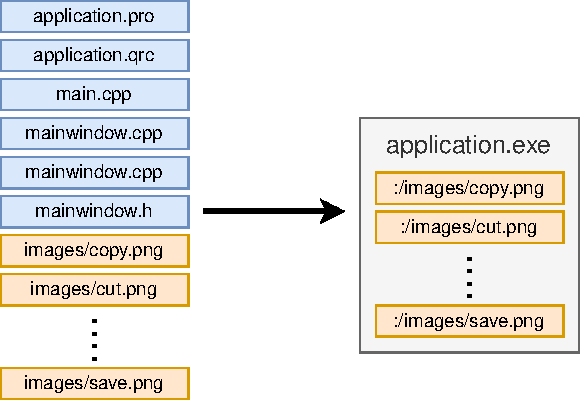
\includegraphics[width=0.5\textwidth]{The_Qt_Resource_System}
\end{figure}

目前,Qt 总是将数据直接存储至可执行程序内,无论是 Windows、macOS 还是 iOS——这些操作系统都提供了内嵌资源的原生支持。这个模式在 Qt 未来的版本中可能会有改变。

\section{压缩}

\hl{rcc} 会尝试压缩资源数据来减少最终生成的二进制文件的磁盘占用。
通常情况下,会通过启发式的检查来决定是否值得进行压缩,并且在无法有效压缩的情况下直接存储未压缩的内容。
您可以使用 \hl{-threshold} 来控制判断阈值,该选项告知 \hl{rcc} 源文件压缩后获得的体积缩减必须不小于该百分比。

\begin{lstlisting}   
rcc -threshold 25 myresources.qrc
\end{lstlisting}

默认值为 \hl{70},意味着压缩后的文件必须比源文件小 70\%(即不大于源文件的 30\% 大小)。

若有需要的话,也可以关闭压缩,这在资源文件中包含已经压缩过的数据时(如 \hl{.png} 文件)非常有用——否则会在编译时浪费 CPU 时间来确认它的确不能被再次压缩。
另一个原因则是无需考虑磁盘占用,并且想让资源在运行时以可直接访问的原始数据存放于内存中,而非需要解压才可使用的压缩数据。
您可以通过命令行参数 \hl{-no-compress} 来实现此目的。

\begin{lstlisting}   
rcc -no-compress myresources.qrc
\end{lstlisting}

\hl{rcc} 同样给予用户控制压缩算法和压缩等级的权限,例如:

\begin{lstlisting}   
rcc -compress 2 -compress-algo zlib myresources.qrc
\end{lstlisting}

另外,也可以在 \hl{.qrc} 文件中 \hl{file} 标签的 \hl{threshold}、\hl{compress} 和 \hl{compress-algo} 属性来进行设置:

\begin{lstlisting}[language=XML]  
<qresource>
    <file compress="1" compress-algo="zstd">data.txt</file>
</qresource>
\end{lstlisting}

上述代码选择 \hl{zstd} 算法,使用压缩等级 1.

\hl{rcc} 支持如下压缩算法和压缩等级:

\begin{compactitem}
\item \hl{best}:使用下述算法中的最优者,并使用其最高压缩等级,以编译时的 CPU 时间为代价来获得最高压缩率。
    此参数在 XML 文件中可用于指明无论 \hl{rcc} 支持何种压缩算法,该文件都应被尽可能地压缩。
\item \hl{zstd}:使用 Zstandard 库进行压缩。有效压缩等级为 1 至 19,1 为最低压缩率(最短 CPU 时间),19 为最高压缩率(最长 CPU 时间)。
 默认等级为 14。特殊值 0 用于告知 \hl{zstd} 库自由选择其默认的压缩率。
\item \hl{zlib}:使用 zlib 库进行压缩。有效压缩等级为 1 至 9,1 为最低压缩率(最短 CPU 时间),9 为最高压缩率(最长 CPU 时间)。
    特殊值 0 代表“无需压缩”,并且不应被使用。默认值为实现定义,通常为 6。
\item \hl{none}:无压缩。该参数等价于 \hl{-no-compress} 选项。
\end{compactitem}

Zstandard 和 zlib 均为可选支持。若运行时未检测到对应的库,则通过 \hl{-compress-algo} 指定该库的操作会报错。
默认情况下,若 \hl{zstd} 可用则使用该算法,否则使用 \hl{zlib}。

\section{在应用程序中使用资源}

在应用程序中,资源路径可用于绝大多数常规文件系统路径的中。
例如,可以传递资源路径而非文件路径至 QIcon,QImage 或 QPixmap 的构造函数:

\begin{lstlisting}[language=C++]
cutAct = new QAction(QIcon(":/images/cut.png"), tr("Cu&t"), this);
\end{lstlisting}

\begin{notice}
Application 范例以了解实际程序中如何使用 Qt 的资源系统来存储图标。
\end{notice}

资源在内存中以资源对象树形式表达,该对象树在程序启动时构建,通过 QFile 来将其路径解析至资源数据。
可通过 \hl{":/"} 初始化 QDir 对象,来从根部遍历该对象树。

Qt 的资源系统支持搜索路径列表概念。若通过 \hl{:} 而非 \hl{:/} 前缀来指定资源,则会通过搜索路径列表来检索该资源。
搜索路径列表在程序启动时为空,可通过 QDir::addSearchPath() 来添加路径。

\section{使用库中的资源}

若在库中包含资源,则需要调用 Q\_INIT\_RESOURCE() 来强制初始化资源,调用参数为 \hl{.qrc} 文件的基本名称,例如

\begin{lstlisting}[language=C++]
MyClass::MyClass() : BaseClass()
{
    Q_INIT_RESOURCE(resources);

    QFile file(":/myfile.dat");
    ...
}
\end{lstlisting}


这确保了在静态链接时,资源数据可被链接至最终的应用程序。
该初始化代码应该紧贴在库中使用资源的位置之前,以确保仅当该库的使用者使用到依赖资源的特性时,才会将资源链接至程序。

\begin{notice}
由于 \hl{rcc} 生成的资源初始化器定义在全局命名空间,Q\_INIT\_RESOURCE() 的调用也必须位于任何命名空间之外。
\end{notice}

若该库包含的资源不在内部使用,而是暴露给库的使用者,则初始化操作需要发生在应用程序代码中,例如:

\begin{lstlisting}[language=C++]
int main(int argc, char *argv[])
{
    QApplication app(argc, argv);
    Q_INIT_RESOURCE(graphlib);
    
    QFile file(":/graph.png");
    ...
    return app.exec();
}    
\end{lstlisting}

如上文所述,此方式确保了资源数据可在静态链接时被链接至最终的应用程序,同时也会在动态链接时触发库的加载动作,如加载插件。

类似地,若想显示地卸载一组资源(因为需要卸载插件,或该资源不再被使用),则可通过调用 Q\_CLEANUP\_RESOURCE() 来强制移除资源,调用参数与上文相同。

\begin{lstlisting}
若资源文件被编译为应用程序的一部分,则不需要使用 Q\_INIT\_RESOURCE() 和 Q\_CLEANUP\_RESOURCE()。
\end{lstlisting}
\chapter{QSql}

QSql 命名空间 里的 各种名样的标识符,已经被运用在 Qt SQL 各个模块中。\href{https://doc.qt.io/qt-5/qsql.html#details}{更多} 

\begin{tabular}{|c|c|p{1.5cm}|}
	\hline
	属性 & 方法 \\
	\hline
	头文件 & \#include <QSql>\\      
	\hline
	qmake & QT += sql\\      
	\hline
\end{tabular}

\section{类型}

\resizebox{\textwidth}{!}{ % Latex表格宽度超出文本宽度
	\begin{tabular}{|c|l|}
		\hline
		&  \\
		\hline
		enum & Location \{ BeforeFirstRow, AfterLastRow \}\\      
		\hline
		enum & NumericalPrecisionPolicy \{ LowPrecisionInt32, LowPrecisionInt64,LowPrecisionDouble,HighPrecision\}\\      
		\hline
		flags & ParamType \\
		\hline 
		enum & ParamTypeFlag \{ In, Out, InOut, Binary \} \\ 
		\hline
		enum & TableType \{ Tables, SystemTables, Views, AllTables \}\\
		\hline
	\end{tabular}
}

细节的介绍 

查看 \href{https://doc.qt.io/qt-5/qtsql-index.html}{Qt SQL}

\section{类型 文档}

enum QSql::Location


此枚举类型描述特殊的sql导航位置


\begin{tabular}{|c|c|c|}
	\hline
	常量	& 值 & 介绍 \\
	\hline
	QSql::BeforeFirstRow&-1&在第一个记录之前\\
	\hline
	QSql::AfterLastRow&-2&在最后一个记录之后\\
	\hline
\end{tabular}

\begin{seeAlso}
\href{https://doc.qt.io/qt-5/qsqlquery.html#at}{QSqlQuery::at()}
\end{seeAlso}

enum QSql::NumericalPrecisionPolicy


数据库中的数值可以比它们对应的C++类型更精确。此枚举列出在应用程序中表示此类值的策略。


\resizebox{\textwidth}{!}{ % Latex表格宽度超出文本宽度
	\begin{tabular}{|c|c|c|}
		\hline
		常量	& 值 & 介绍 \\
		\hline
		QSql::LowPrecisionInt32	&0x01 &对于32位的整形数值。在浮点数的情况下,小数部分将会被舍去。\\
		\hline
		QSql::LowPrecisionInt64	&0x02 &对于64位的整形数值。在浮点数的情况下,小数部分将会被舍去。\\
		\hline
		QSql::LowPrecisionDouble&0x04 &强制双精度值。这个默认的规则\\
		\hline
		QSql::HighPrecision	&0&字符串将会维技精度\\
		\hline
	\end{tabular}
}

\begin{notice}
如果特定的驱动发生溢出,这是一个真实行为。像 Oracle数据库在这种情形下,就会返回一个错误。
\end{notice}

enum QSql::ParamTypeFlag


flags QSql::ParamType


这个枚举用于指定绑定参数的类型

\begin{tabular}{|l|l|l|}
	\hline
	常量	& 值 & 介绍 \\
	\hline
	QSql::In&0x00000001&这个参数被用于向数据库里写入数据\\
	\hline
	QSql::Out&0x00000002&这个参数被用于向数据库里获得数据\\
	\hline
	QSql::InOut&In | Out&这个参数被用于向数据库里写入数据;使用 查询 来向数据库里,重写数据\\
	\hline
	QSql::Binary&0x00000004&如果您想 显示数据为 原始的二进制数据,那么必须是 OR'd 和其他的标志一 起使用\\
	\hline
\end{tabular}

类型参数 类型定义为 \href{https://doc.qt.io/qt-5/qflags.html}{QFlags}. 它被存放在 一个 OR与 类型参数标志的值 的组合。





\chapter{QSqlDatabase}

QSqlDatabase 类 用于处理数据库的连接

\begin{tabular}{|c|c|}
	\hline
	属性 & 方法 \\
	\hline
	头文件 & \#include <QSqlDatabase>\\      
	\hline
	qmake & QT += sql\\      
	\hline
\end{tabular}


\href{https://doc.qt.io/qt-5/qsqldatabase-members.html}{列出所有的成员,包括继承成员}

\section{公共类型}

\resizebox{\textwidth}{!}{ % Latex表格宽度超出文本宽度
\begin{tabular}{|r|l|}
\hline
返回值 & 函数名 \\
\hline
 & QSqlDatabase(const QSqlDatabase \&other) \\ 
\hline
 & QSqlDatabase()\\
\hline
QSqlDatabase \&	&operator=(const QSqlDatabase \&other)\\
\hline
 & ~QSqlDatabase()\\
\hline
void& close()\\
\hline
bool&commit()\\
\hline
QString	&connectOptions() const\\
\hline
QString	&connectionName() const\\
\hline
QString	&databaseName() const\\
\hline
QSqlDriver *&	driver() const\\
\hline
QString	&driverName() const\\
\hline
QSqlQuery&	exec(const QString \&query = QString()) const\\
\hline
QString	&hostName() const\\
\hline
bool	&isOpen() const\\
\hline
bool	&isOpenError() const\\
\hline
bool	&isValid() const\\
\hline
QSqlError&	lastError() const\\
\hline
QSql::NumericalPrecisionPolicy & numericalPrecisionPolicy() const\\
\hline
bool	&open()\\
\hline
bool&	open(const QString \&user, const QString \&password)\\
\hline
QString&	password() const\\
\hline
int	&port() const\\
\hline
QSqlIndex&	primaryIndex(const QString \&tablename) const\\
\hline
QSqlRecord&	record(const QString \&tablename) const\\
\hline
bool	&rollback()\\
\hline
void	&setConnectOptions(const QString \&options = QString())\\
\hline
void	&setDatabaseName(const QString \&name)\\
\hline
void	&setHostName(const QString \&host)\\
\hline
void	& setNumericalPrecisionPolicy(QSql::NumericalPrecisionPolicy    precisionPolicy)\\
\hline
void	&setPassword(const QString \&password)\\
\hline
void	&setPort(int port)\\
\hline
void	&setUserName(const QString \&name)\\
\hline
QStringList	&tables(QSql::TableType type = QSql::Tables) const\\
\hline
bool&	transaction()\\
\hline
QString	&userName() const\\
\hline
\end{tabular}
}

\section{静态公共成员}

\resizebox{\textwidth}{!}{ % Latex表格宽度超出文本宽度
\begin{tabular}{|r|l|}
	\hline
	返回值 & 函数名 \\
	\hline
	QSqlDatabase&	addDatabase(const QString \&type, const QString \&connectionName = QLatin1String(defaultConnection))\\
		\hline
	QSqlDatabase&	addDatabase(QSqlDriver *driver, const QString \&connectionName = QLatin1String(defaultConnection))\\
		\hline
	QSqlDatabase&	cloneDatabase(const QSqlDatabase \&other, const QString \&connectionName)\\
		\hline
	QSqlDatabase&	cloneDatabase(const QString \&other, const QString \&connectionName)\\
		\hline
	QStringList&	connectionNames()\\
		\hline
	bool&	contains(const QString \&connectionName = QLatin1String(defaultConnection))\\
		\hline
	QSqlDatabase&	database(const QString \&connectionName = QLatin1String(defaultConnection), bool open = true)\\
		\hline
	QStringList&	drivers()\\
		\hline
	bool&	isDriverAvailable(const QString \&name)\\
		\hline
	void&	registerSqlDriver(const QString \&name, QSqlDriverCreatorBase *creator)\\
		\hline
	void&	removeDatabase(const QString \&connectionName)\\
	\hline
\end{tabular}
}

\section{受保护的成员函数}

\begin{tabular}{|r|l|}
	\hline
	返回值 & 函数名 \\
	\hline
	&QSqlDatabase(QSqlDriver *driver)\\
	\hline
	&QSqlDatabase(const QString \&type)\\
	\hline
\end{tabular}


\section{详细的介绍}

QSqlDatabase 类提供接口用于数据库的连接 。一个 QSqlDatabase 实例对象表示连接。 这个连接提供 数据库 所需要的 驱动,这个驱动来自于 QSqlDriver。 换而言之,您可以实现自己的数据库驱动,通过继承 QSqlDriver。查看\href{https://doc.qt.io/qt-5/sql-driver.html#how-to-write-your-own-database-driver}{如何实现自己的数据库驱动}来获取更多的信息。

通过调用一个静态的 addDatabase()函数,来创建一个连接(即:实例化一个QSqlDatabase类),并且可以指定驱动或者驱动类型去使用(依赖于数据库的类型 )和 一个连接的名称。 一个连接是通过它自已的名称,而不是通过数据库的名称去连接的。对于一个数据库您可以有多个连接。QSqlDatabase 也支持默认连接,您可以不 传递连接名参数给 addDatabase() 来创建 它。随后,这个默认连接假定您 在调用任何静态函数情况下,而不去指定连接名称。 下面的一段代码片段展示了 如何去创建 和打开一个默认连接,去连接 PostgreSQL 数据库:

\begin{lstlisting}[language=C++]
QSqlDatabase db = QSqlDatabase::database();
\end{lstlisting}

QSqlDatabase是一个值类。通过一个 QSqlDatabase 实例对数据库连接所做的操作将影响表示相同连接的其他 QSqlDatabase 实例。 使用 cloneDatabase() 在基于已存在数据库的连接 来 创建 独立的数据库的连接。

\begin{notice}[警告]
强烈建议不要将QSqlDatabase的拷贝作为类成员,因为这将阻止关闭时正确清理实例。 如果需要访问已经存在QSqlDatabase,应该使用database()访问。如果您选择使用作为成员变量的QSqlDatabase,则需要在删除QCoreApplication实例之前删除它,否则可能会导致未定义的行为。
\end{notice}

如果您想创建多个数据库连接,可以调用 addDatabase(), 并且给一个独一无二的参数(即:连接名称)。使用 带有连接名的database() 函数,来获取该连接。使用 带有连接名的removeDatabase() 函数,来删除 一个连接。如果尝试删除由其他QSqlDatabase对象引用的连接,QSqlDatabase将输出警告。可以使用 \href{https://github.com/QtDocumentCN/QtDocumentCN/blob/master/Src/S/QSqlDatabase/QSqlDatabase.md#static-bool-qsqldatabasecontainsconst-qstring-connectionname--qlatin1stringdefaultconnection}{contains()}查看给定的连接名是否在连接列表中。


\begin{tabular}{|c|c|}
	\hline	
		& 一些实用的方法\\
	\hline
	\href{https://github.com/QtDocumentCN/QtDocumentCN/blob/master/Src/S/QSqlDatabase/QSqlDatabase.md#qstringlist-qsqldatabasetablesqsqltabletype-type--qsqltables-const}{tables()} &	返回 数据表的列表\\
		\hline
	\href{https://github.com/QtDocumentCN/QtDocumentCN/blob/master/Src/S/QSqlDatabase/QSqlDatabase.md#qsqlindex-qsqldatabaseprimaryindexconst-qstring-tablename-const}{primaryIndex()} &返回数据表的主索引\\
		\hline
	\href{URL}{record()} &	返回数据表字段的元信息\\
		\hline
	\href{URL}{transaction()} &开始一个事务\\
		\hline
	\href{URL}{commit()}&	保存并完成一个事务\\
		\hline
	\href{URL}{rollback()}&	取消一个事务\\
		\hline
	\href{URL}{hasFeature()}&	检查驱动程序是否支持事务\\
		\hline
	\href{URL}{lastError()}	&返回有关上一个错误的信息\\
		\hline
	\href{URL}{drivers()}	&返回可用的数据库驱动名称\\
		\hline
	\href{URL}{isDriverAvailable()}	&检查特定驱动程序是否可用\\
		\hline
	\href{URL}{registerSqlDriver()}	&注册自定义驱动程序\\
		\hline
\end{tabular}

\begin{notice}
QSqlDatabase::exec() 方法已经被弃用。请使用 QSqlQuery::exec()
\end{notice}

\begin{notice}
使用事务时,必须在创建查询之前启动事务。
\end{notice}

\section{成员函数文档}

[protected] QSqlDatabase::QSqlDatabase(QSqlDriver *driver)

这是一个重载函数

使用给定驱动程序来创建连接

[protected] QSqlDatabase::QSqlDatabase(const \href{https://github.com/QtDocumentCN/QtDocumentCN/blob/master/Src/S/QString/QString.md}{QString} \&type)

这是一个重载函数

通过引用所给的数据库驱动类型来创建一个连接。如果不给定 数据库驱动类型 ,那么这个数据库连接将会没有什么作用。

当前可用的驱动类型:

\begin{tabular}{|r|l|}
	\hline	
	驱动类别& 介绍\\
	\hline
	QDB2&	IBM DB2\\
		\hline
	QIBASE	&Borland InterBase 驱动\\
		\hline
	QMYSQL	&MySQL 驱动\\
		\hline
	QOCI	&Oracle 调用的接口驱动\\
		\hline
	QODBC	&ODBC 驱动 (包含 Microsoft SQL Server)\\
		\hline
	QPSQL	&PostgreSQL 驱动\\
		\hline
	QSQLITE	&SQLite 第三版本 或者 以上\\
		\hline
	QSQLITE2&	SQLite 第二版本\\
		\hline
	QTDS	&Sybase Adaptive Server\\
	\hline
\end{tabular}

其他第三方驱动程序,包括自己自定义的驱动程序,都可以动态加载。

\begin{notice}[另请参阅]
\href{https://doc.qt.io/qt-5/sql-driver.html}{SQL Database Drivers}, \href{https://github.com/QtDocumentCN/QtDocumentCN/blob/master/Src/S/QSqlDatabase/QSqlDatabase.md#static-void-qsqldatabaseregistersqldriverconst-qstring-name-qsqldrivercreatorbase-creator}{registerSqlDriver()} 和 \href{https://github.com/QtDocumentCN/QtDocumentCN/blob/master/Src/S/QSqlDatabase/QSqlDatabase.md#static-qstringlist-qsqldatabasedrivers}{drivers()}。
\end{notice}


QSqlDatabase::QSqlDatabase(const QSqlDatabase \&other)

创建一个其它的副本

QSqlDatabase::QSqlDatabase()
创建一个 无效的 QSqlDatabase 空对象。
使用\href{https://github.com/QtDocumentCN/QtDocumentCN/blob/master/Src/S/QSqlDatabase/QSqlDatabase.md#static-qsqldatabase-qsqldatabaseadddatabaseconst-qstring-type-const-qstring-connectionname--qlatin1stringdefaultconnection}{addDatabase()},  \href{https://github.com/QtDocumentCN/QtDocumentCN/blob/master/Src/S/QSqlDatabase/QSqlDatabase.md#static-void-qsqldatabaseremovedatabaseconst-qstring-connectionname}{removeDatabase()} 和\href{https://github.com/QtDocumentCN/QtDocumentCN/blob/master/Src/S/QSqlDatabase/QSqlDatabase.md#static-qsqldatabase-qsqldatabasedatabaseconst-qstring-connectionname--qlatin1stringdefaultconnection-bool-open--true}{database()} 来获得一个有效的 QSqlDatabase 对象。

QSqlDatabase \&QSqlDatabase::operator=(const QSqlDatabase \&other)

给这个对象赋一个其他其他对象的值

QSqlDatabase::~QSqlDatabase()

销毁这个对象,并且释放所有配置的资源 注意: 当最后的连接被销毁,这个折构函数就会暗中的调用 close()函数,去删除这个数据库的其他连接。


\begin{notice}[另请参阅 ]
\href{https://github.com/QtDocumentCN/QtDocumentCN/blob/master/Src/S/QSqlDatabase/QSqlDatabase.md#void-qsqldatabaseclose}{close()}。
\end{notice}



[static] QSqlDatabase QSqlDatabase::addDatabase(const QString \&type,const QString \&connectionName = QLatin1String(defaultConnection))

使用驱动程序类型和连接名称,将数据库添加到数据库连接列表中。如果存在相同的连接名,那么这个连接将会被删除。

通过引用连接名,来返回一个新的连接。

如果数据库的类别不存在或者没有被加载,那么 isValid()函数将会返回 false

如果我们没有指定连接名参数,那么应用程序就会返回默认连接。 如果我们提供了连接名参数,那么可以使用database(connectionName) 函数来获取该连接。

\begin{notice}[警告]
如果您指定了 相同的连接名参数,那么就会替换之前的那个相同的连接。如果您多次调用这个函数而不指定 连接名参数,则默认连接将被替换。
\end{notice}


在使用连接之前,它必须经过初始化。比如: 调用下面一些或者全部 \href{https://github.com/QtDocumentCN/QtDocumentCN/blob/master/Src/S/QSqlDatabase/QSqlDatabase.md#void-qsqldatabasesetdatabasenameconst-qstring-name}{setDatabaseName()} 、 \href{https://github.com/QtDocumentCN/QtDocumentCN/blob/master/Src/S/QSqlDatabase/QSqlDatabase.md#void-qsqldatabasesetusernameconst-qstring-name}{setUserName()}、 \href{https://github.com/QtDocumentCN/QtDocumentCN/blob/master/Src/S/QSqlDatabase/QSqlDatabase.md#void-qsqldatabasesetpasswordconst-qstring-password}{setPassword()} 、 \href{https://github.com/QtDocumentCN/QtDocumentCN/blob/master/Src/S/QSqlDatabase/QSqlDatabase.md#void-qsqldatabasesethostnameconst-qstring-host}{setHostName()}、 \href{https://github.com/QtDocumentCN/QtDocumentCN/blob/master/Src/S/QSqlDatabase/QSqlDatabase.md#void-qsqldatabasesetportint-port}{setPort()} 和 \href{https://github.com/QtDocumentCN/QtDocumentCN/blob/master/Src/S/QSqlDatabase/QSqlDatabase.md#void-qsqldatabasesetconnectoptionsconst-qstring-options--qstring}{setConnectOptions()},并最终调用 \href{https://github.com/QtDocumentCN/QtDocumentCN/blob/master/Src/S/QSqlDatabase/QSqlDatabase.md#bool-qsqldatabaseopen}{open()}



\begin{notice}
这个函数是线程安全的
\end{notice}


\begin{notice}[另请查阅]
\href{https://github.com/QtDocumentCN/QtDocumentCN/blob/master/Src/S/QSqlDatabase/QSqlDatabase.md#static-qsqldatabase-qsqldatabasedatabaseconst-qstring-connectionname--qlatin1stringdefaultconnection-bool-open--true}{database()}, \href{https://github.com/QtDocumentCN/QtDocumentCN/blob/master/Src/S/QSqlDatabase/QSqlDatabase.md#static-void-qsqldatabaseremovedatabaseconst-qstring-connectionname}{removeDatabase()} 以及 \href{https://doc.qt.io/qt-5/threads-modules.html#threads-and-the-sql-module}{ 线程和SQL 单元}。
\end{notice}


[static] QSqlDatabase QSqlDatabase::addDatabase(QSqlDriver *driver, const QString \&connectionName = QLatin1String(defaultConnection))

这个重载函数是非常有用的,当您想创建一个带有\href{https://doc.qt.io/qt-5/qsqldriver.html}{驱动} 连接时,您可以实例化它。有可能您想拥有自己的数据库驱动,或者去实例化 Qt自带的驱动。如果您真的想这样做,我非常建议您把驱动的代码导入到您的应用程序中。例如,您可用自已的 QPSQL 驱动来创建一个 PostgreSQL 连接,像下面这样:

\begin{lstlisting}[language=C++]
PGconn *con = PQconnectdb("host=server user=bart password=simpson dbname=springfield");
QPSQLDriver *drv = new QPSQLDriver(con);
QSqlDatabase db = QSqlDatabase::addDatabase(drv); // 产生成新的默认连接
QSqlQuery query;
query.exec("SELECT NAME, ID FROM STAFF");	
\end{lstlisting}

上面的代码用于设置一个 PostgreSQL 连接和实例化一个 QPSQLDriver 对象。接下来,addDatabase() 被调用产生一个已知的连接,以便于它可以使用 Qt SQL 相关的类。Qt假定您已经打开了数据库连接,当使用连接句柄(或一组句柄)实例化驱动程序时。

\begin{notice}
我们假设qtdir是安装Qt的目录。假定您的PostgreSQL头文件己经包含在搜索路径中,然后这里才能引用所需要的PostgreSQL客户端库和去实例化QPSQLDriver对象。
\end{notice}



请记住,必须将数据库客户端库到您的程序里。确保客户端库在您的链接器的搜索路径中,并且像下面这样添加到您的 .pro 文件里:

\begin{lstlisting}[language=C++]
unix:LIBS += -lpq
win32:LIBS += libpqdll.lib
\end{lstlisting}

这里介绍了所有驱动支持的方法。只有驱动的构造参数有所不同。列举了一个关于 Qt附带的程序,以及它们的源代码文件,和它们的构造函数参数的列表:

\resizebox{\textwidth}{!}{ % Latex表格宽度超出文本宽度
\begin{tabular}{|l|l|l|l|}
	\hline
	驱动	&类名	& 构造器参数	& 用于导入的文件\\
	\hline
QPSQL	&QPSQLDriver	&PGconn *connection	&qsql\_psql.cpp \\
\hline
QMYSQL	&QMYSQLDriver	&MYSQL *connection	&qsql\_mysql.cpp\\
\hline
QOCI	&QOCIDriver	&OCIEnv *environment, OCISvcCtx *serviceContext	&qsql\_oci.cpp\\
\hline
QODBC	&QODBCDriver	&SQLHANDLE environment, SQLHANDLE connection	&qsql\_odbc.cpp\\
\hline
QDB2	&QDB2	&SQLHANDLE environment, SQLHANDLE connection	&qsql\_db2.cpp\\
\hline
QTDS	&QTDSDriver	&LOGINREC *loginRecord, DBPROCESS *dbProcess, const QString \&hostName	&qsql\_tds.cpp\\
\hline
QSQLITE	&QSQLiteDriver	&sqlite *connection	&qsql\_sqlite.cpp\\
\hline
QIBASE	&QIBaseDriver	&isc\_db\_handle connection	&qsql\_ibase.cpp\\
 
	\hline
\end{tabular}}

当构造用于为内部查询创建新连接的QTDSDriver时,需要主机名(或服务名)。这是为了防止在同时使用多个QSqlQuery对象时发生阻塞。


\begin{notice}[警告]
我们假设添加一个存在连接名的连接时,这个新添加的连接将会替换另一个。 
\end{notice}


\begin{notice}[警告]
	 SQL框架拥有驱动程序的所有权。它不能被删除。可以使用removeDatabase(),去删除这个连接。 另请参阅drivers()
\end{notice}



[protected] QSqlDatabase QSqlDatabase::cloneDatabase(const QString \&other, const QString \&connectionName)

克隆其他数据库连接并将其存储为connectionName。原始数据库中的所有设置,例如databaseName()、hostName()等,都会被复制。如果其他数据库无效,则不执行任何操作。返回最新被创建的数据库连接。



\begin{notice}[警告]
这个新的连接不能被打开。您必须调用 open(),才能使用这个新的连接。
\end{notice}


[static] QSqlDatabase QSqlDatabase::cloneDatabase(const QString \&other, const QString \&connectionName)
这是个重载函数。

克隆其他数据库连接并将其存储为connectionName。原始数据库中的所有设置,例如databaseName()、hostName()等,都会被复制。如果其他数据库无效,则不执行任何操作。返回最新被创建的数据库连接。



\begin{notice}
这个新的连接不能被打开。您必须调用 open(),才能使用这个新的连接。
\end{notice}

当我们在另一个线程克隆这个数据库,这个重载是非常有用的。

qt5.13中引入了这个函数。

void QSqlDatabase::close()

关闭数据库连接,释放获取的所有资源,并使与数据库一起使用的任何现有QSqlQuery对象无效

这个函数也会影响它的QSqlDatabase对象副本。

另请参阅 removeDatabase()

bool QSqlDatabase::commit()
如果驱动支持事务和一个transaction()已经被启动,那就可以提交一个事务到这个数据库中。如果这个操作成功,就会返回 true。否则返回 false。

注意: 对于一些数据库,如果对数据库使用SELECT进行查询操作,将会提交失败并且返回false。在执行提交之前,使查询处于非活动状态。

调用 lastError() 函数获取错误信息。

另请参阅 QSqlQuery::isActive(), QSqlDriver::hasFeature(),和 rollback()。

QString QSqlDatabase::connectOptions() const
返回用于此连接的连接选项字符串。这个字符串可能是空。

另请参阅 setConnectOptions()

QString QSqlDatabase::connectionName() const
返回连接名,它有可能为空。

注意: 这个连接名不是 数据库名

qt4.4 中引入了这个函数。

另请参阅 addDatabase()

[static] QStringList QSqlDatabase::connectionNames()
返回包含所有连接名称的列表。

注意: 这个函数是线程安全的。

另请参阅 contains(),database(), 和 线程和SQL模块

[static] bool QSqlDatabase::contains(const QString \&connectionName = QLatin1String(defaultConnection))


如果所给的连接名,包含在所给的数据库连接列表里,那么就返回 true;否则返回 false。

注意: 这个函数是 线程安全的

另请参阅 connectionNames(), database() 和 线程和SQL模块。

[static] QSqlDatabase QSqlDatabase::database(const QString \&connectionName = QLatin1String(defaultConnection), bool open = true)


返回一个调用 connectionName 参数的数据库连接。这个数据库连接使用之前,必须已经通过 addDatabase() 函数进行添加。如果open为true(默认值),并且数据库连接尚未打开,则现在打开它。如果未指定连接名参数,则使用默认连接。如果连接名不存在数据库列表中,那么将会返回一个非法的连接。

注意: 这个函数是 线程安全的

另请参阅 isOpen() 和 线程和SQL模块。

QString QSqlDatabase::databaseName() const


返回连接的连接数据库名称,当然它也可能是空的。

注意: 这个数据库名不是连接名

另请参阅 setDatabaseName()。

QSqlDriver *QSqlDatabase::driver() const


返回被使用的数据库连接的所使用的数据库驱动。

另请参阅 addDatabase() 和 drivers()

QString QSqlDatabase::driverName() const


返回连接的驱动名称

另请参阅 addDatabase() 和 driver()

[static] QStringList QSqlDatabase::drivers()


返回一个可使用的数据库驱动列表 另请参阅 registerSqlDriver()

QSqlQuery QSqlDatabase::exec(const QString \&query = QString()) const


在这个数据库里执行 SQL 表达式和 返回一个 QSqhttps://doc.qt.io/qt-5/qsqlquery.html 对象。使用 lastError() 来获取错误的信息。

如果查询为空,则返回一个空的、无效的查询。并且 lastError()。

另请参阅 QSqlQuery 和 lastError()。

QString QSqlDatabase::hostName() const


返回连接的主机名;它有可能为空。

另请参阅 setHostName()

[static] bool QSqlDatabase::isDriverAvailable(const QString \&name)


如果调用一个叫 name 的驱动,是可以使用的,那么就返回 true;反之返回 false。

另请参阅 drivers()。

bool QSqlDatabase::isOpen() const


如果当前数据库连接是打开的,那么就返回 true,否则返回 false。

bool QSqlDatabase::isOpenError() const


如果打开数据库的连接有错误,那么就返回 true,否则返回 false。可以调用 lastError() 函数去获取相关的错误信息。

bool QSqlDatabase::isValid() const


如果 QSqlDatabase() 有一个有效的驱动,那么就返回 true。

例子:

\begin{lstlisting}[language=C++]
QSqlDatabase db;
qDebug() << db.isValid();    // 返回 false

db = QSqlDatabase::database("sales");
qDebug() << db.isValid();    // 如果 "sales" 连接存在,就返回 true

QSqlDatabase::removeDatabase("sales");
qDebug() << db.isValid();    // 返回 false
\end{lstlisting}

\href{https://doc.qt.io/qt-5/qsqlerror.html}{QSqlError} QSqlDatabase::lastError() const

返回这个数据库出现的最新错误信息。

使用 QSqlQuery::lastError() 函数来获取一个单个查询上的错误。

另请参阅 QSqlError and QSqlQuery::lastError()。

QSql::NumericalPrecisionPolicyQSqlDatabase::numericalPrecisionPolicy() const
返回数据库连接的当前默认精度策略。

qt4.6中引入了这个函数。

另请参阅 QSql::NumericalPrecisionPolicy, setNumericalPrecisionPolicy()、

QSqlQuery::numericalPrecisionPolicy() 和 QSqlQuery::setNumericalPrecisionPolicy()。

bool QSqlDatabase::open()


使用当前连接值打开数据库连接。如果操作成功就返回 true; 反之返回 false。可以调用 lastError()来获取错误的信息。

另请参阅 lastError()、 setDatabaseName()、setUserName()、

setPassword()、setHostName()、setPort()和 setConnectOptions()。

bool QSqlDatabase::open(const QString \&user, const QString \&password)


这是一个重载函数。

使用所给的 username 和 password 两个参数,打开数据连接,如果成功就返回 true; 反之返回 false。使用 [lastError()]QSqlDatabase.md\#qsqlerror-qsqldatabaselasterror-const) 来获取错误的信息。

这个函数不存放所给的 password 参数,相反的它会把 password 参数直接传给驱动用于打连接,然后销毁这个参数。

另请参阅 lastError()。

QString QSqlDatabase::password() const


返回连接的密码。如果没有使用setPassword() 函数进行密码的设置 并且 没有调用 open() 以及 没有使用密码,那么就返回空的字符串。

另请参阅 setPassword()

int QSqlDatabase::port() const


返回连接的端口号。如果端口号没有设置,那么这个值就是未定义的。

另请参阅 setPort()


QSqlIndex QSqlDatabase::primaryIndex(const QString \&tablename) const


返回所给表格名的索引。如果索引不存在,那么就返回一个空的 QSqlIndex

注意: 如果表在创建时没有被引用,一些驱动程序(如 QPSQL 驱动程序)可能要求您以小写的形式传递表格名。

查看关于 Qt SQL driver 文档的更多信息。

另请参阅 tables() 和 record()。

QSqlRecord QSqlDatabase::record(const QString \&tablename) const


返回一个QSqlRecord,其中填充了名为tablename的表(或视图)中所有字段的名称。字段在记录中出现的顺序未定义。如果没有这样的表格(或者视图)存在,将会返回一个空的记录。

注意: 如果表在创建时没有被引用,一些驱动程序(如 QPSQL 驱动程序)可能要求您以小写的形式传递表格名。

查看 Qt SQL driver 文档的更多信息。

[static] void QSqlDatabase::registerSqlDriver(const QString \&name, QSqlDriverCreatorBase *creator)


这个函数在 SQL框架中注册一个名为 name 的新 SQL 驱动程序。这个是非常有用的,如果您有一个自定义的驱动,并且您并不想把它编译作为一个插件。

例如:


\begin{lstlisting}[language=C++]
QSqlDatabase::registerSqlDriver("MYDRIVER", new QSqlDriverCreator<QSqlDriver>);
QVERIFY(QSqlDatabase::drivers().contains("MYDRIVER"));
QSqlDatabase db = QSqlDatabase::addDatabase("MYDRIVER");
QVERIFY(db.isValid());
\end{lstlisting}

QSqlDatabase拥有 creator 指针的所有权,因此您不能自己删除它。

另请参阅 drivers()。

[static] void QSqlDatabase::removeDatabase(const QString \&connectionName)


从数据库列表中,删除一个叫 connectionName 数据库连接。

警告: 不应在数据库连接上打开查询的情况下调用此函数,否则将发生资源泄漏。

\clearpage

例子:

\begin{lstlisting}[language=C++]
// 错误
QSqlDatabase db = QSqlDatabase::database("sales");
QSqlQuery query("SELECT NAME, DOB FROM EMPLOYEES", db);
QSqlDatabase::removeDatabase("sales"); // 将会输出警告
// “db”现在是一个悬而未决的无效数据库连接,
// “查询”包含无效的结果集
\end{lstlisting}


正确的做法:

\begin{lstlisting}[language=C++]
{
    QSqlDatabase db = QSqlDatabase::database("sales");
    QSqlQuery query("SELECT NAME, DOB FROM EMPLOYEES", db);
}
// “db”和“query”都被销毁,因为它们超出了范围
QSqlDatabase::removeDatabase("sales"); // 正确的
\end{lstlisting}

如果要删除默认连接,这个连接可能是通过调用 addDatabase() 函数而创建的,但未指定连接名称,可以通过对database()返回的数据库调用connectionName() 来检索默认连接名称。注意,如果没有创建默认数据库,将返回一个无效的数据库。

注意: 这个函数是线程安全的

另请查阅 database(),connectionName(),和 线程和SQL模块。

bool QSqlDatabase::rollback()


在数据库里回滚一个事务,如果驱动支持一个事务以及一个 transaction() 已经被启动。如果操作成功返回 true。否则返回 false。

注意: 对于某些数据库,如果存在使用数据库进行选择的活动查询,则回滚将失败并返回false。确保在执行回滚操作之前,查询是 非活动 的状态。

调用 lastError() 操作获得错误的相关信息。

另请查阅 QSqlQuery::isActive(),QSqlDriver::hasFeature() 和 commit()。

void QSqlDatabase::setConnectOptions(const QString \&options = QString())


设置一组数据库的具体的可选项。它必须在打之这个连接之前执行这个操作,否则是无效的。另一个可能的原因是调用 QSqlDatabase::setConnectOptions() 去关闭这个连接,并且调用 open() 再次关闭这个连接。

选项字符串的格式是以分号分隔的选项名称,或选项=值对的列表。这个选项依赖于所使用的客户端:

\begin{tabular}{|c|c|c|}
	\hline
    ODBC & MySQL & PostgreSQL \\
	\hline
    SQL\_ATTR\_ACCESS\_MODE & CLIENT\_COMPRESS	& connect\_timeout \\
    \hline
    SQL\_ATTR\_LOGIN\_TIMEOUT & CLIENT\_FOUND\_ROWS &	options \\
    \hline
    SQL\_ATTR\_CONNECTION\_TIMEOUT	& CLIENT\_IGNORE\_SPACE &	tty \\
    \hline
    SQL\_ATTR\_CURRENT\_CATALOG &	CLIENT\_ODBC &	requiressl \\
\hline
    SQL\_ATTR\_METADATA\_ID &	CLIENT\_NO\_SCHEMA&	service \\
\hline
    SQL\_ATTR\_PACKET\_SIZE&	CLIENT\_INTERACTIVE&\\	
\hline
    SQL\_ATTR\_TRACEFILE&	UNIX\_SOCKET&	\\
\hline
    SQL\_ATTR\_TRACE&	MYSQL\_OPT\_RECONNECT& \\	
\hline
    SQL\_ATTR\_CONNECTION\_POOLING	&MYSQL\_OPT\_CONNECT\_TIMEOUT& \\	
\hline
    SQL\_ATTR\_ODBC\_VERSION&	MYSQL\_OPT\_READ\_TIMEOUT&\\	
\hline
                         &MYSQL\_OPT\_WRITE\_TIMEOUT&	\\
\hline
                         &SSL\_KEY&	 \\
\hline
                         &SSL\_CERT&\\	
\hline
                         &SSL\_CA&	\\
\hline
                         &SSL\_CAPATH&\\
\hline
                         &SSL\_CIPHER&\\
	\hline
\end{tabular}

\begin{tabular}{|c|c|c|}
	\hline
	DB2	&OCI	&TDS \\ 
	\hline
	SQL\_ATTR\_ACCESS\_MODE & OCI\_ATTR\_PREFETCH\_ROWS	& 无 \\
	\hline
	SQL\_ATTR\_LOGIN\_TIMEOUT & OCI\_ATTR\_PREFETCH\_MEMORY& \\	
	\hline
\end{tabular}

\begin{tabular}{|c|c|}
	\hline
	\href{https://doc.qt.io/qt-5/qtsql-attribution-sqlite.html#sqlite}{SQLite} & Interbase \\ 
	\hline
	QSQLITE\_BUSY\_TIMEOUT & ISC\_DPB\_LC\_CTYPE \\ 
	\hline
	QSQLITE\_OPEN\_READONLY	& ISC\_DPB\_SQL\_ROLE\_NAME \\ 
	\hline
	QSQLITE\_OPEN\_URI&	\\ 
	\hline
	QSQLITE\_ENABLE\_SHARED\_CACHE	& \\
	\hline
	QSQLITE\_ENABLE\_REGEXP &  \\
	\hline
\end{tabular}

\clearpage

例子:

\begin{lstlisting}[language=C++]
db.setConnectOptions("SSL_KEY=client-key.pem;SSL_CERT=client-cert.pem;SSL_CA=ca-cert.pem;CLIENT_IGNORE_SPACE=1"); // 使用安全套连字进行连接
if (!db.open()) {
	db.setConnectOptions(); // 清除连接的字符串
	// ...
}
// ...
// PostgreSQL 连接
db.setConnectOptions("requiressl=1"); // 确保 PostgreSQL 安全套接字连接
if (!db.open()) {
	db.setConnectOptions(); // 清除可选
	// ...
}
// ...
// ODBC 连接
db.setConnectOptions("SQL_ATTR_ACCESS_MODE=SQL_MODE_READ_ONLY;SQL_ATTR_TRACE=SQL_OPT_TRACE_ON"); // 设置 ODBC 连项
if (!db.open()) {
	db.setConnectOptions(); // 不要尝试去设置这个选项。
	// ...
}
}
\end{lstlisting}

查阅这个客户端库文档,获得更多关于不同可选项的更多信息。

另请查阅 connectOptions()。

void QSqlDatabase::setDatabaseName(const QString \&name)

通过所给的 name 参数来设置所连接的数据库名称。必须在打开连接之前设置数据库名称。 或者,可以调用close()函数关闭连接,设置数据库名称,然后再次调用open() 。

注意: 这个数据库名不是连接名。必须在创建连接对象时将连接名称传递给 addDatabase()。

对于 QSQLITE 驱动,如果数据库名指定的名字不存在,然后它将会创建这个文件,除非您设置了 QSQLITE\_OPEN\_READONLY

此外,可以把 name 参数设置为 :memory:, 可以创建一个临时数据库,该数据库仅在应用程序的生命周期内可用。

对于 QOCI (Oracle) 驱动,这个数据库名是 TNS Service Name。

对于 QODBC 驱动程序,名称可以是DSN,DSN文件名(在这种情况下,文件扩展名必须为.DSN)或者是一个连接字符串。

例如,Microsoft Access 可以使用下面的连接方式来直接打开 .mdb 文件,而不是在 ODBC 管理工具里创建一个 DSN 对象:

\clearpage

\begin{lstlisting}[language=C++]
// ...
QSqlDatabase db = QSqlDatabase::addDatabase("QODBC");
db.setDatabaseName("DRIVER={Microsoft Access Driver (*.mdb, *.accdb)};
FIL={MS Access};DBQ=myaccessfile.mdb");
if (db.open()) {
	// 成功!
}
// ...
\end{lstlisting}

这个没有默认的值

另请查阅 databaseName()、setUserName()、 setPassword()、 setHostName()、 

setPort()、setConnectOptions() 和 open()。


void QSqlDatabase::setHostName(const QString \&host)

通过 host 参数来设置连接的主机名。为了生效,必须在打开连接之前,设置主机名。或者,可以调用close()关闭连接,然后设置主机名,再次调用open()函数。

这个没有默认值。

另请查阅 hostName(), setUserName(), setPassword(),setDatabaseName(),setPort(), setConnectOptions() 和 open()。

void QSqlDatabase::setNumericalPrecisionPolicy(QSql::NumericalPrecisionPolicy precisionPolicy)


设置在此数据库连接上创建的查询使用的默认数值精度策略。

注意: 驱动程序不支持以低精度获取数值,将忽略精度策略。您可以使用 QSqlDriver::hasFeature()来查找一个驱动是否支持这个功能。

注意: 通过 precisionPolicy 来设置这个默认的精度策略,将不会响影任何当前的活动查询。

qt4.6中引入了这个函数。

另请查阅 QSql::NumericalPrecisionPolicy,
numericalPrecisionPolicy(),QSqlQuery::setNumericalPrecisionPolicy 和 QSqlQuery::numericalPrecisionPolicy.

void QSqlDatabase::setPassword(const QString \&password)
通过 password 参数来设置连接的密码。为了生效,必须在打开连接之前来设置密码。或者,您可以调用close()关闭连接,然后设置密码,再次调用open()函数。

这个没有默认值。

警告: 这个函数以明文的形式把密码存放到qt里。 将密码作为参数来避免这个行为,然后使用 open()进行调用。

另请查阅 password(),setUserName(),setDatabaseName(),setHostName(),

setPort(), setConnectOptions()和 open()。

void QSqlDatabase::setPort(int port)

通过port参数设置连接的端口号。为了生效,您必须在打开连接之前,进行端口号的设置。或者,您可以调用close()关闭连接,然后设置端口号,再次调用open()函数

这个没有默认的值。

另请查阅 port(), setUserName(), setPassword(),

setHostName(),setDatabaseName(), setConnectOptions() 和 open()。

void QSqlDatabase::setUserName(const QString \&name)

通过 name 参数来设置连接的用户名。为了生效,必须在打开连接之前设置用户名。或者,您可以调用 close()函数来关闭连接,设置用户,然后再次调用 open()

这个没有默认值。

另请查阅 userName(),setDatabaseName(),setPassword(),

setHostName(),setPort(),setConnectOptions() 和 open()。

QStringList QSqlDatabase::tables(QSql::TableType type = QSql::Tables) const
返回由 parameter type 参数 指定的数据库的表格、系统表和视图的列表。

另请查阅 primaryIndex() 和 record()。

bool QSqlDatabase::transaction()
如果驱动程序支持事务,则在数据库上开始事务。如果操作成功的话,返回 true, 否则返回 false。

另请查阅 QSqlDriver::hasFeature(), commit() 和 rollback()。

QString QSqlDatabase::userName() const
返回连接的用户名; 它也许为空。

另请查阅 setUserName()。


\chapter{QSctpServer}

QSctpServer 提供了一个基于 QSCTP 协议的服务器。

\begin{tabular}{|r|l|}
	\hline
	属性 & 方法 \\
	\hline
	头文件 & \#include <QSctpServer>\\      
	\hline
	qmake & QT += network\\      
	\hline
	引入版本 &	Qt5.8 \\ 
	\hline
继承自	 & QTcpServer \\ 
	\hline
\end{tabular}

该类最初在 Qt5.8 版本时引入 。

\section{公共成员函数}

\begin{tabular}{|r|l|}
	\hline 
	类型	& 函数名 \\ 
	\hline
	& QSctpServer(QObject \emph{*parent} = nullptr)  \\ 
	\hline
	virtual	& $\sim$QSctpServer() \\ 
	\hline
	int	& maximumChannelCount() const  \\ 
	\hline
	QSctpSocket* &	nextPendingDatagramConnection() \\ 
	\hline
	void	& setMaximumChannelCount(int \emph{count}) \\ 
	\hline
\end{tabular}


\section{重写保护成员函数}

\begin{tabular}{|r|l|}
	\hline 
	类型	& 函数名 \\ 
	\hline
	virtual void	& incomingConnection(qintptr \emph{socketDescriptor}) override \\ 
	\hline
\end{tabular}

\section{详细介绍}

SCTP(流控制传输协议)是一种传输层协议,其作用与流行的协议 TCP 和 UDP 类似。像 UDP 一样,
SCTP 也是面向消息的,但是它可以通过与 TCP 类似的拥塞控制来确保消息的可靠性,让消息按顺序传输。
您可以在 QSctpSocket 类文档中找到关于 SCTP 协议的更多的信息。

QSctpServer 是 QTcpServer 的便利子类,它允许您以 TCP 模拟或数据报模式接受传入的 SCTP 套接字连接。

QSctpServer 最常见的用法是构造一个 QSctpServer 类的对象并调用 setMaximumChannelCount() 函数设置该服务器准备支持的最大通道数。
您可以在调用 setMaximumChannelCount() 函数时传入一个负值,这样便可以让服务端在 TCP 模拟模式下运行。
另外,如果在 setMaximumChannelCount() 函数调用时传入0(0也是默认值),
这会指定服务端使用对等端设置的最大通道数目。新的传入连接从服务器套接字描述符继承此数字,
并根据远程端点设置对其进行调整。

在 TCP 模拟模式下,服务端允许客户端使用一条连续的字节流来进行数据传输。
此时 QSctpSocket 的操作模式与普通的 QTcpServer 类似。
您可以调用 nextPendingConnection() 函数将一个待处理的连接作为一个已连接的 QTcpSocket 套字节来接受。
您可以使用该 QTcpSocket 套接字与客户端进行通信。此模式仅能使用基本的 SCTP 协议功能。
套接字在系统层面通过 IP 传输 SCTP 数据包,并通过 QTcpSocket 接口与应用程序进行交互。

与 TCP 模拟模式相反,数据报模式是面向消息的,并且在端点之间提供了多个数据流的完全同时传输。
您可以调用 nextPendingDatagramConnection() 函数将待处理的数据报模式的连接作为一个已连接的 QSctpSocket 套接字接受。


\begin{notice}
WIndows系统不支持该特性。
\end{notice}

\begin{seeAlso}
QTcpServer ,QSctpSocket 和 QAbstractSocket。
\end{seeAlso}

\section{成员函数文档}

QSctpServer::QSctpServer(QObject \emph{*parent} = nullptr)

构造函数。构造一个 QSctpServer 类型的对象并将其设置为数据报模式。

\emph{parent} 参数将传递到 QObject 构造函数中。

\begin{seeAlso}
setMaximumChannelCount(),listen() 和 setSocketDescriptor()。
\end{seeAlso}

[virtual] QSctpServer::$\sim$QSctpServer()

析构函数。
销毁 QSctpServer 类型的对象。
如果服务端仍然在监听客户端连接,该套接字会自动关闭。


\begin{seeAlso}
close()。
\end{seeAlso}

[override virtual protected] void QSctpServer::incomingConnection(qintptr \emph{socketDescriptor})

重写 QTcpServer::incomingConnection(qintptr socketDescriptor) 函数。

int QSctpServer::maximumChannelCount() const

返回套接字能够支持的最大通道数。

如果返回值为0(默认值)意味着支持的最大通道数将由远程端点设置。

如果 QSctpServer 运行在 TCP 模拟模式,该函数返回-1。

\begin{seeAlso}
setMaximumChannelCount()。
\end{seeAlso}

QSctpSocket *QSctpServer::nextPendingDatagramConnection()

将下一个待处理的数据报模式的连接作为一个已连接的 QSctpSocket 对象返回。

数据报模式的连接提供了一个面向消息的、多数据流的通信。

该返回的套接字将作为服务端的子类创建,这意味着当 QSctpServer 对象销毁时,该套接字也将销毁。当您使用完一个对象后显式地删除该对象是一个好的做法,这能避免浪费内存。

如果没有待处理的数据报模式的连接,该函数将返回空。

\begin{notice}
返回的 QSctpSocket 对象不能被其他线程使用。
如果想在其他线程中使用到达的连接,您需要重写 incomingConnection() 函数。
\end{notice}

\begin{seeAlso}
hasPendingConnections() ,nextPendingConnection() 和 QSctpSocket。
\end{seeAlso}

void QSctpServer::setMaximumChannelCount(int \emph{count})

设置在数据报模式下服务端准备支持的最大通道数为 \emph{count} 。

如果 \emph{count} 为 0,服务端将使用其他端点的最大通道数。

如果 \emph{count} 为一个负值,则 QSctpServer 将会在 TCP 模拟模式下运行。

\begin{seeAlso}
maximumChannelCount() 和 QSctpSocket。
\end{seeAlso}
\chapter{QSctpSocket}

QSctpSocket 类提供了一个 SCTP 类型的套接字。

\begin{tabular}{|r|l|}
	\hline
	属性 & 方法 \\
	\hline
	头文件 & \#include <QSctpSocket>\\      
	\hline
	qmake & QT += network\\      
	\hline
	引入 &	Qt5.8 \\ 
	\hline
	父类	 & QTcpSocket \\ 
	\hline
\end{tabular}

该类最初在 Qt5.8 版本时引入 。

\section{公共成员函数}

\begin{tabular}{|r|l|}
	\hline 
	类型	& 函数名 \\ 
	\hline
	& QSctpSocket(QObject *parent = nullptr) \\ 
	\hline
	virtual	& $\sim$QSctpSocket() \\ 
	\hline
	bool	& isInDatagramMode() const \\ 
	\hline
	int	& maximumChannelCount() const \\ 
	\hline
	QNetworkDatagram &	readDatagram() \\ 
	\hline
	void	& setMaximumChannelCount(int \emph{count}) \\ 
	\hline
	bool &	writeDatagram(const QNetworkDatagram \emph{\&datagram}) \\ 
	\hline
\end{tabular}


\section{重写公共成员函数}

\begin{tabular}{|r|l|}
	\hline 
	类型	& 函数名 \\ 
	\hline
	virtual void	& close() override \\ 
	\hline
    virtual void	& disconnectFromHost() override \\ 
	\hline
\end{tabular}


\section{重写保护成员函数}

\begin{tabular}{|r|l|}
	\hline 
	类型	& 函数名 \\ 
	\hline
	virtual qint64	& readData(char \emph{*data}, qint64 \emph{maxSize}) override \\ 
	\hline
    virtual qint64	& readLineData(char \emph{*data}, qint64 \emph{maxlen}) override \\ 
	\hline
\end{tabular}

\section{详细介绍}

SCTP(流控制传输协议)是一种传输层协议,其作用与流行的协议 TCP 和 UDP 类似。 
像 UDP 一样,SCTP 也是面向消息的,但是它可以通过类似 TCP 的拥塞控制来确保消息的可靠性,使消息按顺序传输。

SCTP 是面向连接的协议,它提供端点之间多个数据流的完全同时传输。 
这种多数据流允许通过独立的通道传输数据,因此,如果一个数据流中有数据丢失,则其他数据流的传输将不会受到影响。

作为一个面向消息的传输协议,SCTP 以序列方式传输消息,而不是像 TCP 一样传输连续的字节流。 
像在 UDP 中一样,在 SCTP 中,发送方在一个操作中发送一条消息,
而确切的消息则在一个操作中传递给接收应用程序进程。
 但是与 UDP 不同,消息的传递是有可靠性保证的。

SCTP 还支持多宿主,这意味着连接的端点可以具有一些与其关联的备用 IP 地址,
以便绕过网络故障或变化的条件进行数据传输。

QSctpSocket 是 QTcpSocket 的便利子类,它使您可以通过 SCTP 模拟 TCP 数据流或建立 SCTP 连接以实现可靠的数据报服务。

QSctpSocket 可以在以下两种模式之一中运行:

\begin{compactitem}
\item 连续字节流(TCP 模拟)。
\item 多流数据报模式。
\end{compactitem}

要设置连续字节流模式,您可以首先实例化一个 QSctpSocket 对象并使用一个负值作为参数调用 setMaximumChannelCount() ,
这样就可以将 QSctpSocket 用作常规的缓冲 QTcpSocket 类型套接字使用。 
您可以调用 connectToHost() 来发起与端点的连接,可以调用 write() 和 read() 来与对等方进行消息发送与接收,但是在这种模式下您无法区分消息的边界。

默认情况下,QSctpSocket 使用数据报模式下进行操作。 
在您建立连接之前,请先调用 setMaximumChannelCount() 设置应用程序准备支持的最大通道数。 
此数字是与远程端点协商的参数,其值受操作系统的限制。 默认值0表示使用对等端的值。
如果两个端点都使用默认值,则连接通道的数量取决于系统。 建立连接后,
可以通过调用 readChannelCount() 和 writeChannelCount() 获取实际的通道数。

\begin{cppcode}
 QSctpSocket *socket = new QSctpSocket(this);

socket->setMaxChannelCount(16);
socket->connectToHost(QHostAddress::LocalHost, 1973);

if (socket->waitForConnected(1000)) {
	int inputChannels = socket->readChannelCount();
	int outputChannels = socket->writeChannelCount();

	....
}
\end{cppcode}


在数据报模式,QSctpSocket 为每一个通道单独执行数据报的缓冲操作。
您可以通过调用 writeDatagram() 函数将当前通道的一个数据报加入缓冲队列,
调用 readDatagram() 函数从当前通道读取一个待处理的数据报。

在数据报模式下,允许使用标准的 QIODevice 成员函数 read(),readLine(),
write() 等,其限制与连续字节流模式相同。


\begin{notice}
多通道数据报模式并不被 Windows 操作系统支持。
\end{notice}

\begin{seeAlso}
QSctpServer ,QTcpSocket ,QAbstractSocket。
\end{seeAlso}

\section{成员函数文档}

QSctpSocket::QSctpSocket**(QObject \emph{*parent} = nullptr)

构造函数。
创建一个处于 未连接( UnconnectedState )状态的 QSctpSocket 类型的对象并设置为数据报操作模式。

\begin{seeAlso}
socketType() 和 setMaximumChannelCount() 。
\end{seeAlso}

[virtual] QSctpSocket::$\sim$QSctpSocket()

析构函数。销毁套接字,必要时关闭连接。

\begin{seeAlso}
close()。
\end{seeAlso}

[override virtual] void QSctpSocket::close()

重写 QAbstractSocket::close() 。

[override virtual] void QSctpSocket::disconnectFromHost()

重写 QAbstractSocket::disconnectFromHost() 。

bool QSctpSocket::isInDatagramMode() const

如果该套接字运行在数据报模式则返回 true 。

\begin{seeAlso}
setMaximumChannelCount()。
\end{seeAlso}

int QSctpSocket::maximumChannelCount() const

返回 QSctpSocket 能支持的最大通道数。

如果返回值为0(默认值)意味着连接的通道数由远程端点设置。

如果 QSctpSocket 运行在连续字节流模式则返回-1。

\begin{seeAlso}
setMaximumChannelCount() ,readChannelCount() 和 writeChannelCount() 。
\end{seeAlso}

[override virtual protected] qint64 QSctpSocket::readData(char \emph{*data}, qint64 \emph{maxSize})

重写: QAbstractSocket::readData(char *data, qint64 maxSize).

QNetworkDatagram QSctpSocket::readDatagram()

从当前的读取通道的缓冲区读取一个数据报并将该数据报内容及其发送者的主机地址和端口写入一个 QNetworkDatagram 对象中返回。如果可能,此功能还将尝试确定数据报的目标地址,端口以及接收时的跳数计数,并将这些信息写入到返回的 QNetworkDatagram 对象中。

如果操作失败,将会返回一个无效的 QNetworkDatagram 对象。

\begin{seeAlso}
writeDatagram() ,isInDatagramMode() 和 currentReadChannel() 。
\end{seeAlso}

[override virtual protected] qint64 QSctpSocket::readLineData(char \emph{*data}, qint64 \emph{maxlen})

重写: QAbstractSocket::readLineData(char *data, qint64 maxlen).

void QSctpSocket::setMaximumChannelCount(int \emph{count})

设置该应用程序在数据报模式下将支持的最大通道数为 count 。 如果 count 为0,程序将使用远程端点设置的最大通道支持数。将 count 设置为一个负数时,程序将使用连续字节流模式。

您应该仅在 QSctpSocket 处在未连接( UnconnectedState )状态时调用该函数。

\begin{seeAlso}
maximumChannelCount() ,readChannelCount() 和 writeChannelCount()。
\end{seeAlso}

bool QSctpSocket::writeDatagram(const QNetworkDatagram \&datagram)

将一个数据报写入到当前写出通道的缓冲区。操作成功该函数返回 true ,否则返回 false 。

\begin{seeAlso}
readDatagram() ,isInDatagramMode() 和 currentWriteChannel()。
\end{seeAlso}
\chapter{QSemaphore}

QSemaphore类提供了一个通用的信号量。\href{}{更多内容...}

\begin{tabular}{|r|l|}
	\hline
	属性 & 方法 \\
	\hline
	头文件 & \#include <QSemaphore>\\      
	\hline
	qmake & QT += core\\      
	\hline
\end{tabular}

\begin{warning}
此类中所有函数都是线程安全的。
\end{warning}

\section{公共成员函数}

\begin{tabular}{|r|l|}
	\hline 
	返回类型	& 函数名 \\ 
	\hline 
	& QSemaphore(int \emph{n} = 0) \\ 
	\hline
	& $\sim$QSemaphore() \\
	\hline
	void	& acquire(int \emph{n} = 1) const \\ 
	\hline
	int	& available() const \\ 
	\hline
	void &	release(int \emph{n} = 1) \\
	\hline
	bool &	tryAcquire(int \emph{n} = 1) \\ 
	\hline 
	bool	&tryAcquire(int \emph{n}, int \emph{timeout}) \\ 
	\hline
\end{tabular}


\section{详细描述}

信号量是互斥量的泛化。虽然互斥量只能锁定一次,但可以多次获取信号。信号量通常用于保护一定数量的相同资源。

信号量支持两个基本操作,acquire() 和 release():

\begin{compactitem}[\arr]
\item acquire(n) 尝试获取 n 个资源。如果没有那么多可用资源,调用将被阻塞,直到能够获取。
\item release(n) 释放 n 个资源。
\end{compactitem}

还有 tryAcquire() 函数,如果无法获取资源,它将立即返回;还有一个 available() 函数,可以随时返回可用资源的数量。

例如:

\begin{lstlisting}[language=C++]
QSemaphore sem(5);      // sem.available() == 5

sem.acquire(3);         // sem.available() == 2
sem.acquire(2);         // sem.available() == 0
sem.release(5);         // sem.available() == 5
sem.release(5);         // sem.available() == 10

sem.tryAcquire(1);      // sem.available() == 9, returns true
sem.tryAcquire(250);    // sem.available() == 9, returns false
\end{lstlisting}

信号量的一个典型应用场景,是控制生产者线程和消费者线程对共享循环缓冲区的访问。生产者消费者示例展示了如何使用 QSemaphore 来解决这个问题。

一个非计算信号量(non-computing)的例子是在餐馆就餐。用餐厅里的椅子数初始化信号量。
当人们到达时,他们需要要一个座位。入座后,available() 将减少。当人们离开时,available() 会增加,允许更多的人进入。
如果有一个 10 人的聚会,但是餐馆只有 9 个座位,那这 10 个人会等待空出位置。
但是如果此时有一个 4 人的聚会,那么他们会入座(将可用的座位减少到 5 个,10 人聚会将等待更长时间)。

\begin{seeAlso}
QSemaphoreReleaser,QMutex,QWaitCondition,QThread 和 生产者消费者示例。
\end{seeAlso}

\section{成员类型文档}

QSemaphore::QSemaphore(int \emph{n} = 0)

构造一个信号量并将其保护的资源数量初始化为 \hl{n}(默认为0)。

\begin{seeAlso}
release(),available()。
\end{seeAlso}

QSemaphore::$\sim$QSemaphore()

析构。

\begin{warning}
析构正在使用的信号量可能会导致未定义的行为。
\end{warning}

void QSemaphore::acquire(int \emph{n} = 1)

尝试获取由信号量保护的 n 个资源。如果 \hl{n > available()},则此调用将阻塞,直到有足够的资源可用。

\begin{seeAlso}
release(),available(),tryAcquire()。
\end{seeAlso}

int QSemaphore::available() const

返回信号量当前可用的资源数。返回值永远不会是负数。

\begin{seeAlso}
release(),available()。
\end{seeAlso}

void QSemaphore::release(int \emph{n} = 1)

释放 n 个信号量保护的资源。

这个函数也可以用来“创建”资源。例如:

\begin{lstlisting}[language=C++]
QSemaphore sem(5);      // 信号量保护 5 个资源  sem.avilable() == 5
sem.acquire(5);         // 请求 5 个资源       sem.avilable() == 0
sem.release(5);         // 释放 5 个资源       sem.avilable() == 5
sem.release(10);        // “创建” 10 个新资源  sem.avilable() == 15
\end{lstlisting}

QSemaphoreReleaser 是一个围绕此函数的 RAII 包装器。

\begin{seeAlso}
acquire(),available(),QSemaphoreReleaser。
\end{seeAlso}

bool QSemaphore::tryAcquire(int \emph{n} = 1)

尝试获取由信号量保护的 n 个资源,并在成功时返回 \hl{true}。如果 \hl{available() < n},此调用立即返回 \hl{false},而不获取任何资源。

例如:

\begin{lstlisting}[language=C++]
QSemaphore sem(5);      // sem.available() == 5
sem.tryAcquire(250);    // sem.available() == 5, returns false
sem.tryAcquire(3);      // sem.available() == 2, returns true
\end{lstlisting}

\begin{seeAlso}
acquire()。
\end{seeAlso}

bool QSemaphore::tryAcquire(int \emph{n}, int \emph{timeout})

尝试获取由信号量保护的 n 个资源,并在成功时返回 \hl{true}。如果 \hl{available() < n},此调用将等待 \hl{timeout} 毫秒,以尝试获取。

\begin{notice}
传递一个负数作为超时相当于调用 \hl{acquire()},也就是说,如果 \hl{timeout} 为负数,这个函数将永远等待资源可用。
\end{notice}

例如:

\begin{lstlisting}[language=C++]
QSemaphore sem(5);            // sem.available() == 5
sem.tryAcquire(250, 1000);    // sem.available() == 5, 等待 1000 毫秒,returns false
sem.tryAcquire(3, 30000);     // sem.available() == 2, 立即返回,returns true
\end{lstlisting}

\begin{seeAlso}
acquire()。
\end{seeAlso}


\chapter{QSerialPort}

QSerialPort 类用于访问串口。更多内容...

\begin{tabular}{|r|l|}
	\hline
	属性 & 方法 \\
	\hline
	头文件 & \#include <QSerialPort>\\      
	\hline
	qmake & QT += serialport\\      
	\hline
	父类: & QIODevice \\
	\hline
\end{tabular}

\begin{compactitem}
\item 列出所有成员, 包括子类成员
\item 废弃的类
\end{compactitem}

\begin{notice}
该类中的所有函数均为 reentrant。
\end{notice}

\section{公共成员类型}

\begin{longtable}[l]{|r|m{30em}|}
	\hline 
	类型	& 方法 \\ 
	\hline 
	enum &	BaudRate \{Baud1200, Baud2400, Baud4800, Baud9600, Baud19200, …, UnknownBaud \} \\ 
	\hline
	enum &	DataBits \{ Data5, Data6, Data7, Data8, UnknownDataBits \} \\ 
	\hline
	enum &	Direction \{ Input, Output, AllDirections \} \\ 
	\hline 
	flags& ParamType	Directions \\ 
	\hline 
	enum&	FlowControl \{ NoFlowControl, HardwareControl, SoftwareControl, UnknownFlowControl \} \\ 
	\hline
	enum&	DataBitsParity \{ NoParity, EvenParity, OddParity, SpaceParity, MarkParity, UnknownParity \} \\ 
	\hline
	enum&	PinoutSignal \{ NoSignal, TransmittedDataSignal, ReceivedDataSignal, DataTerminalReadySignal, DataCarrierDetectSignal, …, SecondaryReceivedDataSignal \}\\ 
     \hline 
	flags&	PinoutSignals \\ 
	\hline
	enum&	SerialPortError \{ NoError, DeviceNotFoundError, PermissionError, OpenError, NotOpenError, …, UnknownError \} \\ 
	\hline
	enum&	StopBits \{ OneStop, OneAndHalfStop, TwoStop, UnknownStopBits \} \\ 
	\hline
\end{longtable}


\section{属性}

\begin{tabular}{|r|l|}
\hline
属性名	& 类型  \\
\hline
baudRate &	qint32 \\ 
\hline
breakEnabled	&bool \\ 
\hline
dataBits&	dataBits \\ 
\hline
dataTerminalReady	&bool \\ 
\hline
error&	SerialPortError \\ 
\hline
flowControl&	FlowControl \\ 
\hline
parity	&Parity \\ 
\hline
requestToSend&	bool \\ 
\hline
stopBits	&StopBits \\ 
\hline
\end{tabular}

\section{公共成员函数}

\begin{longtable}[l]{|r|m{25em}|}
\hline
返回类型&	函数名 \\ 
\hline
&QSerialPort(const QSerialPortInfo \&serialPortInfo, QObject *parent = nullptr) \\
\hline
&QSerialPort(const QString \&name, QObject *parent = nullptr) \\ 
\hline
&[QSerialPort](QObject *parent = nullptr) \\ 
\hline
virtual&	$\sim$QSerialPort() \\ 
\hline
qint32&	baudRate(QSerialPort::Directions directions = AllDirections) const \\ 
\hline
bool&	clear(QSerialPort::Directions directions = AllDirections) \\ 
\hline
void&	clearError() \\ 
\hline
QSerialPort::DataBits&	dataBits() const \\ 
\hline
QSerialPort::SerialPortError&	error() const \\ 
\hline
QSerialPort::FlowControl&	flowControl() const \\ 
\hline
bool&	flush() \\ 
\hline
QSerialPort::Handle	&handle() const \\ 
\hline
bool&	isBreakEnabled() const \\ 
\hline
bool&	isDataTerminalReady()  \\ 
\hline
bool&	isRequestToSend() \\ 
\hline
QSerialPort::Parity	&parity() const \\ 
\hline
QSerialPort::PinoutSignals	&pinoutSignals() \\ 
\hline
QString	&portName() const \\ 
\hline
qint64	&readBufferSize() const \\ 
\hline
bool	&sendBreak(int duration = 0) \\ 
\hline
bool	&setBaudRate(qint32 baudRate, QSerialPort::Directions directions = AllDirections) \\ 
\hline
bool	&setBreakEnabled(bool set = true) \\ 
\hline
bool	&setDataBits(QSerialPort::DataBits dataBits) \\ 
\hline
bool	&setDataTerminalReady(bool set) \\ 
\hline
bool	&setFlowControl(QSerialPort::FlowControl flowControl) \\ 
\hline
bool	&setParity(QSerialPort::Parity parity) \\ 
\hline
void	&setPort(const QSerialPortInfo \&serialPortInfo) \\ 
\hline
void	&setPortName(const QString \&name) \\ 
\hline
void	&setReadBufferSize(qint64 size) \\ 
\hline
bool	&setRequestToSend(bool set) \\ 
\hline
bool	&setStopBits(QSerialPort::StopBits stopBits) \\ 
\hline
QSerialPort::StopBits &	stopBits() const \\ 
\hline
\end{longtable}


\section{重写公共成员函数}

\begin{longtable}[l]{|r|m{25em}|}
	\hline
	返回类型&	函数名 \\ 
	\hline
	virtual bool 	&atEnd() const override \\ 
	\hline
virtual qint64&	bytesAvailable() const override \\ 
\hline
virtual qint64&	bytesToWrite() const override \\ 
\hline
virtual bool&	canReadLine() const override \\ 
\hline
virtual void&	close() override \\ 
\hline
virtual bool	&isSequential() const override \\ 
\hline
virtual bool&	open(QIODevice::OpenMode mode) override \\ 
\hline
virtual bool&	waitForBytesWritten(int msecs = 30000) override \\ 
\hline
virtual bool&	waitForReadyRead(int msecs = 30000) override \\
	\hline
\end{longtable}


\section{信号}

\begin{longtable}[l]{|r|l|}
\hline
返回类型&	函数名 \\ 
\hline
void	&baudRateChanged(qint32 baudRate, QSerialPort::Directions directions) \\ 
\hline
void	&breakEnabledChanged(bool set) \\ 
\hline
void	&dataBitsChanged(QSerialPort::DataBits dataBits) \\ 
\hline
void	&dataTerminalReadyChanged(bool set) \\ 
\hline
void	&errorOccurred(QSerialPort::SerialPortError error) \\  
\hline
void&	flowControlChanged(QSerialPort::FlowControl flow) \\ 
\hline
void&	parityChanged(QSerialPort::Parity parity) \\ 
\hline
void&	requestToSendChanged(bool set) \\ 
\hline
void&	stopBitsChanged(QSerialPort::StopBits stopBits) \\ 
\hline
\end{longtable}

\section{重写保护成员函数}

\begin{tabular}{|r|l|}
\hline
返回类型&	函数名 \\ 
\hline
virtual qint64&	readData(char \emph{*data}, qint64 \emph{maxSize}) override \\
\hline
virtual qint64&	readLineData(char \emph{*data}, qint64 \emph{maxSize}) override \\ 
\hline
virtual qint64&	writeData(const char \emph{*data}, qint64 \emph{maxSize}) override \\ 
\hline
\end{tabular}



\section{详细描述}

您可以使用 QSerialPortInfo 帮助类来获取可用串口的信息,这个类可以枚举系统中的所有串口,当您想使用某个串口时,使用这个类可以获得正确的串口名。可以通过把 QSerialPortInfo 类实例对象作为参数传递给 setPort() 或 setPortName() 方法来指定串口设备。

串口设置完毕以后,可以使用 open() 方法以只读 (r/o)、只写 (w/o)、读写 (r/w) 模式打开串口。

\begin{notice}
串口总是以独占访问的方式打开,即其它进程或线程无法访问已经打开的串口。
\end{notice}

请使用 close() 方法来关闭串口或取消串口读写操作。

串口打开以后,QSerialPort 会检查串口当前的配置并初始化。
您可以使用 setBaudRate(), setDataBits(), setParity(), setStopBits(), 和 setFlowControl() 方法重新配置串口。

QSerialPort::dataTerminalReady 和 QSerialPort::requestToSend 属性用来设置串口引脚信号,还可以使用 pinoutSignals() 方法来查询串口引脚信号。

当串口准备好时,可以用 read() 或 write() 方法来读写串口。
您还可以使用 readLine() 和 readAll() 这样的便捷方法读写串口。
如果数据没有一次读完,剩下的数据会被接下来有新数据被添加至 QSerialPort 内部读缓冲器时再读出。
您可以使用 setReadBufferSize() 方法来设置串口读缓冲区的大小。

QSerialPort 提供了一组函数来暂停线程调用直到触发特定的信号。这些函数可以用来阻塞串口:

\begin{compactitem}
\item waitForReadyRead() 函数阻塞线程调用直到串口有新数据准备读出
\item waitForBytesWritten() 函数阻塞线程调用直到有新数据被写进串口
\end{compactitem}

阻塞串口代码示例:

\begin{cppcode}
int numRead = 0, numReadTotal = 0;
char buffer[50];

for (;;) {
    numRead  = serial.read(buffer, 50);

    // Do whatever with the array

    numReadTotal += numRead;
    if (numRead == 0 && !serial.waitForReadyRead())
        break;
}
\end{cppcode}

如果 waitForReadyRead() 返回 false,说明串口连接已经关闭或者有错误出现。

如果串口出现错误,QSerialPort 将会发射 errorOccurred() 信号。
您还可以调用 error() 方法来查询串口最近一次出现错误的类型。

\begin{notice}
在 QSerialPort 中,并非所有的错误都是以操作系统平台无关的方式处理。
诸如帧、奇偶校验、终止条件这样的错误需要由应用程序代码来处理,可能需要使用设备描述符中的操作系统相关的 ioctls 和(或)解析串口数据流中的字节填充。
\end{notice}

编程阻塞串口与编程非阻塞串口完全不同。阻塞串口不需要事件循环,通常会让编程更简单。
然而,在图形用户界面程序中,阻塞串口应该仅用于非图形用户界面线程,这样做可以避免用户界面卡顿。

若想更深入了解这方面内容,请参考 example 中的例程。

QSerialPort 类还可以与 QTextStream 和 QDataStream 的流运算符(<<()和>>())一起使用。
有一点需要注意:在使用流运算符 >>() 之前请确保串口缓冲区有足够多的数据可读。

\begin{seeAlso}
QSerialPortInfo。
\end{seeAlso}

\section{成员类型文档}

enum QSerialPort::BaudRate

该枚举描述了串口通信波特率。

\begin{notice}
该枚举仅列出了最常用的串口通信波特率。
\end{notice}


\begin{longtable}[l]{|r|c|m{20em}|}
\hline
常量	&值&	描述 \\ 
\hline
QSerialPort::Baud1200 &	1200&	1200 比特/秒 \\ 
\hline
QSerialPort::Baud2400	&2400&	2400 比特/秒 \\ 
\hline
QSerialPort::Baud4800	&4800&	4800 比特/秒 \\ 
\hline
QSerialPort::Baud9600	&9600&	9600 比特/秒 \\ 
\hline
QSerialPort::Baud19200	&19200&	19200 比特/秒 \\ 
\hline
QSerialPort::Baud38400	&38400	&38400 比特/秒 \\ 
\hline
QSerialPort::Baud57600	&57600	&57600 比特/秒 \\ 
\hline
QSerialPort::Baud115200&	115200&	115200 比特/秒 \\ 
\hline
QSerialPort::UnknownBaud	&-1	&波特率未知。这个值已经废弃了。此处保留是为了兼容旧的代码。
 强烈建议您在新开发的代码中不使用这个值 \\ 
\hline
\end{longtable}

\begin{seeAlso}
QSerialPort::baudRate。
\end{seeAlso}

enum QSerialPort::DataBits

该枚举描述了每个字符所使用的数据比特数。

\begin{longtable}[l]{|r|c|m{20em}|}
\hline
常量	&值&	描述 \\ 
\hline 
QSerialPort::Data5 &	5&	每个字符用5比特表示,用于波特码,常见于旧式设备,例如电传打字机 \\ 
\hline
QSerialPort::Data6	&6&	每个字符用6比特表示,很少这样用 \\ 
\hline
QSerialPort::Data7&	7&	每个字符用7比特表示,用于ASCII码,常见于旧式设备,例如电传打字机 \\ 
\hline
QSerialPort::Data8	&8	&每个字符用8比特表示,大部分数据采用此格式,因为1个字节包含8比特。它在新应用中广泛使用 \\ 
\hline
QSerialPort::UnknownDataBits&	-1&	比特数未知。这个值已经废弃了。此处保留是为了兼容旧的代码。强烈建议您在新开发的代码中不使用这个值 \\ 
	\hline
\end{longtable}

\begin{seeAlso}
QSerialPort::dataBits。
\end{seeAlso}

enum QSerialPort::Direction

flags QSerialPort::Directions

该枚举描述了串口数据传输方向。

\begin{notice}
在某些操作系统中(例如类 POSIX 系统),该枚举对串口的输入/输出波特率单独设置。
\end{notice}

\begin{tabular}{|r|c|l|}
\hline
常量	&值&	描述 \\ 
\hline 
QSerialPort::Input	& 1 &	输入方向 \\ 
\hline
QSerialPort::Output	 &2	 &输出方向 \\ 
\hline
QSerialPort::AllDirections&	Input&	Output \\
\hline
\end{tabular}


方向类型是 QFlags 的类型定义(typedef),它保存了方向值的 OR 组合。

enum QSerialPort::FlowControl

该枚举描述了串口使用的流控制方式。

\begin{tabular}{|r|c|m{20em}|}
\hline
常量	&值&	描述 \\ 
\hline 
QSerialPort::NoFlowControl&	0	&没有流控制 \\ 
\hline
QSerialPort::HardwareControl&	1&	硬件流控制 (RTS/CTS) \\ 
\hline
QSerialPort::SoftwareControl&	2	&软件流控制 (XON/XOFF) \\ 
\hline
QSerialPort::UnknownFlowControl	&-1 &	流控制未知。这个值已经废弃了。此处保留是为了兼容旧的代码。强烈建议您在新开发的代码中不使用这个值 \\ 
\hline
\end{tabular}

\begin{seeAlso}
QSerialPort::flowControl。
\end{seeAlso}

enum QSerial::Parity

该枚举描述了串口使用的奇偶校验模式。

\begin{tabular}{|r|c|m{22em}|}
\hline
常量	&值&	描述 \\ 
\hline 
QSerialPort::NoParity	&0&	没有奇偶校验。这是最常见的奇偶校验设置。错误检测由通信协议完成 \\ 
\hline 
QSerialPort::EvenParity&	2	&每个字符包含1比特奇偶校验,字符比特数为偶数(含奇偶校验位) \\ 
\hline
QSerialPort::OddParity&	3	&每个字符包含1比特奇偶校验,字符比特数为奇数(含奇偶校验位)。它确保了每个字符至少有一次状态转换 \\ 
\hline
QSerialPort::SpaceParity&	4	&间隔奇偶校验。奇偶校验位在间隔信号中发送。它不提供错误检测信息 \\ 
\hline
QSerialPort::MarkParity	&5&	标志奇偶校验。奇偶校验位总是被置为标志信号(逻辑 1)。它不提供错误检测信息 \\ 
\hline
QSerialPort::UnknownParity&	-1	&奇偶校验未知。这个值已经废弃了。此处保留是为了兼容旧的代码。强烈建议您在新开发的代码中不使用这个值 \\ 
\hline
\end{tabular}

\begin{seeAlso}
QSerialPort::parity。
\end{seeAlso}

enum QSerialPort::PinoutSignal

flags QSerialPort::PinoutSignals

该枚举用于描述串口引脚信号。

\begin{longtable}[l]{|r|c|m{9em}|}
\hline
常量	&值&	描述 \\ 
\hline 
QSerialPort::NoSignal	&0x00&	无信号 \\ 
\hline
QSerialPort::TransmittedDataSignal&	0x01&	TxD (发送数据)。这个值已经废弃了。此处保留是为了兼容旧的代码。强烈建议您在新开发的代码中不使用这个值 \\
\hline
QSerialPort::ReceivedDataSignal	&0x02	&RxD (接收数据)。这个值已经废弃了。此处保留是为了兼容旧的代码。强烈建议您在新开发的代码中不使用这个值\\
\hline
QSerialPort::DataTerminalReadySignal	&0x04&	DTR (数据终端就绪) \\ 
\hline
QSerialPort::DataCarrierDetectSignal	&0x08&	DCD (数据载波检测) \\ 
\hline
QSerialPort::DataSetReadySignal	&0x10	&DSR (数据就绪) \\ 
\hline
QSerialPort::RingIndicatorSignal&	0x20&	RNG (振铃提示) \\ 
\hline
QSerialPort::RequestToSendSignal	&0x40&	RTS (请求发送) \\ 
\hline
QSerialPort::ClearToSendSignal	&0x80&	CTS (清除发送) \\
\hline 
QSerialPort::SecondaryTransmittedDataSignal	&0x100&	STD (辅助发送数据) \\
\hline
QSerialPort::SecondaryReceivedDataSignal&	0x200	&SRD (辅助接收数据) \\ 
\hline
\end{longtable}

PinoutSignals类型是 QFlags 的类型定义(typedef),它保存了PinoutSignal值的 OR 组合。

\begin{seeAlso}
pinoutSignals(), QSerialPort::dataTerminalReady, 和 QSerialPort::requestToSend。
\end{seeAlso}

enum QSerialPort::SerialPortError

该枚举描述了 QSerialPort::error 属性的错误类型。

\begin{longtable}[l]{|r|c|m{9em}|}
	\hline
	常量	&值&	描述 \\ 
	\hline 
	QSerialPort::NoError &	0 &	没有错误 \\ 
	\hline
	QSerialPort::DeviceNotFoundError &	1 &	尝试打开一个不存在的串口设备 \\ 
	\hline
	QSerialPort::PermissionError 	&2 	&其它进程试图打开一个已经开启的串口设备或者用户没有足够的权限打开串口 \\ 
	\hline
	QSerialPort::OpenError &	3& 	在当前对象中试图打开一个已经开启的串口 \\ 
	\hline
	QSerialPort::NotOpenError 	&13 &	在串口未开启时执行某个操作。这个值从 QtSerialPort 5.2 开始使用 \\
	\hline 
	QSerialPort::ParityError &	4 &	读串口时硬件检测到奇偶校验错误。这个值已经废弃了。强烈建议您在新开发的代码中不使用这个值 \\ 
	\hline
	QSerialPort::FramingError &	5 &	读串口时硬件检测到帧错误。这个值已经废弃了。强烈建议您在新开发的代码中不使用这个值 \\ 
	\hline
	QSerialPort::BreakConditionError &	6 &	串口输入线上检测到终止条件。这个值已经废弃了。强烈建议您在新开发的代码中不使用这个值 \\ 
	\hline
	QSerialPort::WriteError &	7 	&写串口时出现的 I/O 错误 \\ 
	\hline
	QSerialPort::ReadError &	8 &	读串口时出现的 I/O 错误 \\ 
\hline
	QSerialPort::ResourceError 	&9 	&当资源无法访问时出现的 I/O 错误。例如:当串口设备意外断开时 \\ 
	\hline
	QSerialPort::UnsupportedOperationError& 	10 &	操作系统禁止或不支持请求的串口操作 \\ 
	\hline
	QSerialPort::TimeoutError 	&12 &	超时错误。这个值从 QtSerialPort 5.2 开始使用 \\ 
	\hline
	QSerialPort::UnknownError &	11 &	未知错误 \\ 
	\hline
\end{longtable}


enum QSerialPort::StopBits

该枚举描述了串口停止位的比特数。

\begin{tabular}{|r|c|m{15em}|}
	\hline
	常量	&值&	描述 \\ 
	\hline 
	QSerialPort::OneStop 	&1& 	1比特停止位 \\ 
	\hline
	QSerialPort::OneAndHalfStop &	3 &	1.5比特停止位(仅适用于Windows系统) \\ 
	\hline
	QSerialPort::TwoStop &	2 	&2比特停止位 \\ 
	\hline
	QSerialPort::UnknownStopBits &	-1& 	停止位比特数未知。这个值已经废弃了。此处保留是为了兼容旧的代码。强烈建议您在新开发的代码中不使用这个值 \\ 
   \hline
\end{tabular}

\begin{seeAlso}
QSerialPort::stopBits。
\end{seeAlso}

\section{成员属性文档}


baudRate : qint32

该属性为串口在指定方向(输入/输出)上的通信波特率。

如果串口波特率设置成功或者打开串口前设置好波特率,那么返回true,否则返回false并且把错误码置1。该错误码可以通过读取 QSerialPort::error 属性的值获得。您可以使用枚举 QSerialPort::BaudRate 或者任何 qint32 型正整数值设置串口通信波特率。

\begin{notice}
如果在打开串口前设置该属性,那么真实的串口设置将会在串口打开后,在 QSerialPort::open() 方法中自动完成。
\end{notice}

\begin{warning}
所有操作系统均支持 AllDirections 标志位设置,但 Windows 系统仅支持这种模式。
\end{warning}

\begin{warning}
在 Windows 系统中无论串口输入还是输出,其波特率均相同。
\end{warning}

该属性的默认值为 Baud9600,即 9600 比特/秒。

存取函数:

\begin{tabular}{|r|m{25em}|}
\hline
返回类型 &	函数名 \\ 
\hline
qint32 	&baudRate(QSerialPort::Directions \emph{directions} = AllDirections) const \\ 
\hline
bool 	&setBaudRate(qint32 baudRate, QSerialPort::Directions \emph{directions} = AllDirections) \\ 
\hline
\end{tabular} 

通知信号:

\begin{tabular}{|r|m{25em}|}
\hline
返回类型 &	函数名 \\
\hline
void 	& baudRateChanged(qint32 baudRate, QSerialPort::Directions directions) \\ 
\hline
\end{tabular} 

breakEnabled : bool

该属性为串口是否终止传输的标志位。

若串口终止通信,则该属性为 true,否则为 false。

注意: 在设置或访问该属性前串口必须已经打开,否则返回 false 并且 NotOpenError 错误码将被置 1。这一点与常规的 Qt 类属性设置不同。然而,这种差异性源于该属性是通过操作系统内核与串口硬件之间的交互来设置的,因此 Qt 串口类属性与其它 Qt 类属性不完全等同。

该属性从 Qt 5.5 开始使用。

存取函数:

\begin{tabular}{|r|l|}
\hline
返回类型 	& 函数名 \\ 
\hline 
bool 	&isBreakEnabled() const \\ 
\hline
bool &	setBreakEnabled(bool set = true) \\ 
\hline
\end{tabular}


%%%%%%%%%%%%%%%%%%%%%%%%%%%%%%%%%%%%%%%%%%%%%%%%%%%%%%%%%%%%

通知信号:

\begin{tabular}{|r|l|}
\hline
返回类型  &	函数名 \\ 
\hline
void &	breakEnabledChanged(bool set) \\ 
\hline
\end{tabular}

dataBits : DataBits 

该属性为串口数据帧中的比特数。

若设置成功或者打开串口前设置好该属性,那么返回true,否则返回false并且把错误码置1。该错误码可以通过读取 QSerialPort::error 属性的值获得。

注意: 如果在打开串口前设置该属性,那么真实的串口设置将会在串口打开后,在 QSerialPort::open() 方法中自动完成。

该属性的默认值为 Data8,即数据帧为8比特。

存取函数:

\begin{tabular}{|r|l|}
\hline
返回类型  &	函数名 \\ 
\hline
QSerialPort::DataBits  &	dataBits() const \\
\hline
bool &	setDataBits(QSerialPort::DataBits dataBits) \\ 
\hline
\end{tabular}

通知信号:

\begin{tabular}{|r|l|}
	\hline
	返回类型  &	函数名 \\ 
	\hline
	void 	& dataBitsChanged(QSerialPort::DataBits dataBits) \\ 
	\hline
\end{tabular}

dataTerminalReady : bool

该属性为串口信号线 DTR 的状态(高或低)。

如果串口信号线 DTR 被置为高电平,则返回true,否则返回false.

注意: 在设置或访问该属性前串口必须已经打开,否则返回 false 并且 NotOpenError 错误码将被置 1。

存取函数:

\begin{tabular}{|r|l|}
\hline
返回类型  &	函数名 \\ 
\hline
bool &	isDataTerminalReady() \\ 
\hline
bool &	setDataTerminalReady(bool set) \\ 
\hline
\end{tabular}
 
通知信号:

\begin{tabular}{|r|l|}
	\hline
	返回类型  &	函数名 \\ 
	\hline
	void 	& dataTerminalReadyChanged(bool set) \\ 
	\hline
\end{tabular}

另请参阅 pinoutSignals()。

error : SerialPortError

该属性为串口的错误码。

串口设备会返回一个错误码。
例如:如果函数 open() 返回false,或者读/写操作返回-1,该属性可以用来判断操作失败的原因。

当调用clearError()函数后,错误码会被置为默认值 QSerialPort::NoError.

存取函数:

\begin{tabular}{|r|l|}
	\hline
	返回类型  &	函数名 \\ 
	\hline
	QSerialPort::SerialPortError 	&error() const \\ 
	\hline
void 	&clearError() \\ 
	\hline
\end{tabular}



flowControl : FlowControl

该属性为串口使用的流控制方式。

若设置成功或者打开串口前设置好该属性,那么返回true,否则返回false并且把错误码置1。该错误码可以通过读取 QSerialPort::error 属性的值获得。

注意: 如果在打开串口前设置该属性,那么真实的串口设置将会在串口打开后,在 QSerialPort::open() 方法中自动完成。

该属性的默认值为 NoFlowControl,即没有流控制。

存取函数:

\begin{tabular}{|r|l|}
	\hline
返回类型 &	函数名 \\ 
\hline
QSerialPort::FlowControl &	flowControl() const \\ 
\hline
bool &	setFlowControl(QSerialPort::FlowControl flowControl) \\ 
\hline
\end{tabular}


通知信号:

\begin{tabular}{|r|l|}
\hline
返回类型 &函数名 \\ 
\hline
void 	&flowControlChanged(QSerialPort::FlowControl flow) \\ 
\hline
\end{tabular}

parity : Parity 

该属性为串口使用的奇偶校验模式。

若设置成功或者打开串口前设置好该属性,那么返回true,否则返回false并且把错误码置1。该错误码可以通过读取 QSerialPort::error 属性的值获得。

\begin{notice}
如果在打开串口前设置该属性,那么真实的串口设置将会在串口打开后,在 QSerialPort::open() 方法中自动完成。
\end{notice}

该属性的默认值为 NoParity,即没有奇偶校验。

存取函数:

\begin{tabular}{|r|l|}
\hline
返回类型 &函数名 \\ 
\hline
QSerialPort::Parity &	parity() const \\
\hline
bool &	setParity(QSerialPort::Parity parity) \\ 
\hline
\end{tabular}

通知信号:

\begin{tabular}{|r|l|}
	\hline
	返回类型 &函数名 \\ 
	\hline
	void 	& parityChanged(QSerialPort::Parity parity) \\
\hline
\end{tabular}


requestToSend : bool

该属性为串口信号线 RTS 的状态(高或低)。

如果串口信号线 RTS 被置为高电平,则返回true,否则返回false.

\begin{notice}
在设置或访问该属性前串口必须已经打开,否则返回 false 并且 NotOpenError 错误码将被置 1。
\end{notice}

\begin{notice}
在 HardwareControl 模式下直接控制 RTS 信号会出错, 错误码 UnsupportedOperationError 会被置1,因为 RTS 信号由驱动自动控制。
\end{notice}

存取函数:

\begin{tabular}{|r|l|}
\hline
返回类型 &	函数名 \\ 
\hline
bool &	isRequestToSend() \\ 
\hline
bool 	& setRequestToSend(bool set) \\ 
\hline
\end{tabular}
\chapter{QTcpServer}

QTcpServer 类提供了一个基于 TCP 协议的服务器。

\begin{tabular}{|r|l|}
	\hline
	属性 & 方法 \\
	\hline
	头文件 & \#include <QTcpServer>\\      
	\hline
	qmake & QT += network\\      
	\hline
	父类	  & QObject \\ 
	\hline
    子类	 & QSctpServer \\ 
	\hline
\end{tabular}


\begin{notice}
该类的所有成员函数都是可重入的。
\end{notice}

\section{公共成员函数}

\begin{longtable}{|r|l|}
	\hline
		& QTcpServer(QObject *parent = nullptr) \\
	\hline
	 virtual	& $\sim$QTcpServer() \\ 
	\hline
void	 & close() \\ 
\hline
QString	& errorString() const \\
\hline
virtual bool	& hasPendingConnections() const \\ 
\hline
bool	& isListening() const \\ 
\hline
bool	& listen(const QHostAddress \&address = QHostAddress::Any, quint16 port = 0) \\ 
\hline
int	& maxPendingConnections() const \\
\hline
virtual QTcpSocket *	& nextPendingConnection()\\
\hline
void	 & pauseAccepting() \\ 
\hline
QNetworkProxy	& proxy() const\\
\hline
void	 & resumeAccepting()\\
\hline
QHostAddress & 	serverAddress() const\\
\hline
QAbstractSocket::SocketError	 & serverError() const \\
\hline
quint16	 & serverPort() const\\
\hline
void	 & setMaxPendingConnections(int numConnections)\\
\hline
void	 & setProxy(const QNetworkProxy \&networkProxy)\\
\hline
bool	& setSocketDescriptor(qintptr socketDescriptor)\\
\hline
qintptr	& socketDescriptor() const\\
\hline
bool	& waitForNewConnection(int msec = 0, bool *timedOut = nullptr)\\
	\hline
\end{longtable}

\section{信号}

\begin{tabular}{|r|l|}
	\hline
	类型	 & 函数名 \\
	\hline
void	v & acceptError(QAbstractSocket::SocketError \emph{socketError}) \\
\hline
void	 & newConnection() \\
	\hline 
\end{tabular}

\section{保护成员函数}

\begin{tabular}{|r|l|}
	\hline
	类型	 & 函数名 \\
	\hline
void	 &  addPendingConnection(QTcpSocket \emph{*socket}) \\ 
\hline
virtual void	 & incomingConnection(qintptr \emph{socketDescriptor}) \\ 
	\hline 
\end{tabular}

\section{详细介绍}

这个类使“用Qt编写一个接受 TCP 链接的服务器”的构想成为可能。您可以为 QTcpServer 指定一个端口或者让它自动选一个。您也可以令 QTcpServer 仅监听一个指定的地址或者让它监听这台机器上的所有地址。

调用 listen() 函数来为到达的连接建立服务器监听。每次当有新的客户端连接到这个服务端时,QTcpServer 都会发出 newConnection() 信号。

调用 nextPendingConnection() 函数接受一个连接到 QTcpServer 的待处理连接。 该函数会返回一个处于已连接( QAbstractSocket::ConnectedState )状态的 QTcpSocket ,您可以使用这个 QTcpSocket 与客户端进行通信。

如果发生错误,serverError() 函数会返回该错误的类型。 您可以调用 errorString() 函数来获取一个能让人看懂的错误描述。

当服务器正在监听连接时,服务器所监听的地址和端口可以通过 serverAddress() 和 serverPort() 函数来获取。

调用 close() 函数后 QTcpServer 会停止监听到达的连接。

另外您也可以在 QTcpSocket 类文档和Qt官方给出的 Fortune Server Example ,Threaded Fortune Server Example ,Loopback Example 和 Torrent Example 示例文档中找到相关信息。

\section{成员函数文档}

QTcpServer::QTcpServer(QObject  \emph{*parent}= nullptr)

构造函数。构造一个 QTcpServer 对象。

\emph{parent} 参数将传递到 QObject 的构造函数中。

\begin{notice}[另请参阅]
listen() 和 setSocketDescriptor()。
\end{notice}


% gog 

[SIGNAL] void QTcpServer::acceptError(QAbstractSocket::SocketError \emph{socketError})

当接受一个新的连接时出错,QTcpServer 会发送此信号。 socketError 参数描述了该错误的类型。

该函数最早在Qt5.0版本引入。

\begin{notice}[另请参阅]
pauseAccepting() 和 resumeAccepting()。
\end{notice}

[SIGNAL] void QTcpServer::newConnection()

每当有新的连接可用时,QTcpServer 都会发送该消息。

\begin{notice}[另请参阅]
hasPendingConnections() 和 nextPendingConnection()。
\end{notice}

[virtual] QTcpServer::$\sim$QTcpServer()

析构函数。销毁 QTcpServer 对象。如果服务器正在监听连接,套接字会自动关闭。

在服务端删除之前,所有仍处于连接状态的客户端 QTcpSocket 都必须断开连接或者重新指定父类。

\begin{notice}[另请参阅]
 close() 。
\end{notice}


[protected] void QTcpServer::addPendingConnection(QTcpSocket  \emph{*socket})

该函数由 QTcpServer::incomingConnection() 函数调用,作用是添加 socket 到待处理连接列表中。

\begin{notice}
如果您不想破坏连接处理机制,请不要忘记从重新实现的 incomingConnection() 中调用此成员。
\end{notice}

该函数最初在Qt4.7版本引入。

\begin{notice}[另请参阅]
incomingConnection() 
\end{notice}

void QTcpServer::close()

关闭服务器。服务器将不再监听到达的连接。

\begin{notice}[另请参阅]
 listen() 
\end{notice}

QString QTcpServer::errorString() const

将最后一个出现的错误的相关信息按照适合人阅读的形式返回。


\begin{notice}[另请参阅]
serverError() 
\end{notice}


[virtual] bool QTcpServer::hasPendingConnections() const

当服务端有待处理的连接时该函数返回 true ,否则返回 false 。

\begin{notice}[另请参阅]
nextPendingConnection() 和 setMaxPendingConnections()。
\end{notice}








\chapter{QTcpSocket}

QTcpSocket 提供了一个 TCP 类型的套接字。

\begin{tabular}{|r|l|}
	\hline
	属性 & 方法 \\
	\hline
	头文件 & \#include <QTcpSocket>\\      
	\hline
	qmake & QT += network\\      
	\hline
	父类	  & QAbstractSocket \\ 
	\hline
    子类	 & QSctpSocket 和 QSslSocket \\ 
	\hline
\end{tabular}


\begin{notice}
QTcpSocket类中所有的函数都是可重入函数。
\end{notice}

\section{公共成员函数}

\begin{tabular}{|r|l|}
	\hline
		& QTcpSocket(QObject  \emph{*parent} = nullptr) \\
	\hline
	 virtual	& $\sim$QTcpSocket() \\ 
	\hline
\end{tabular}

\section{详细描述}




TCP(传输控制协议)是一种可靠的,面向流,面向连接的传输协议。 它特别适合连续数据传输。

QTcpSocket 是继承自 QAbstractSocket 的一个便利子类,它允许您建立 TCP 连接并传输数据流。您可以阅读 QAbstractSocket 文档获取详细信息。

\begin{notice}
	无法在 QIODevice::Unbuffered 模式下打开 TCP 套接字。
\end{notice}



\begin{notice}[另请查阅]
QTcpServer, QUdpSocket, QNetworkAccessManager, Fortune Server Example, Fortune Client Example, Threaded Fortune Server Example, Blocking Fortune Client Example, Loopback Example 和  and Torrent Example。
\end{notice}



\section{成员函数文档}

QTcpSocket::QTcpSocket(QObject  \emph{*parent} = nullptr)


构造函数。创建一个 QTcpSocket 类型的对象。该对象创建后初始状态为未连接( UnconnectedState )状态。


函数中父对象参数 \emph{parent} 传递给 QObject 的构造函数。

\begin{notice}[另请查阅]
\href{https://doc.qt.io/qt-5/qabstractsocket.html#socketType}{socketType()}。
\end{notice}



\emph{[virtual]}QTcpSocket::$\sim$QTcpSocket()

析构函数。销毁套接字,必要时关闭连接。

\begin{notice}[另请查阅]
\href{https://doc.qt.io/qt-5/qabstractsocket.html#close}{close()}。
\end{notice}








\chapter{QTimer}

QTimer提供了重复和信号槽的定时器。

\begin{tabular}{|r|l|}
	\hline
	属性 & 方法 \\
	\hline
	头文件 & \#include <QTimer>\\      
	\hline
	qmake & QT += core\\      
	\hline
	继承	  & QObject \\ 
	\hline
\end{tabular}

\section{属性}

\begin{tabular}{|r|l|}
	\hline
属性名	 & 类型 \\ 
\hline
active	& const bool\\
\hline
singleShot	& bool\\
\hline
interval &	int\\
\hline
timeType	& Qt::TimerType\\
\hline
remainingTime &	const int\\
	\hline
\end{tabular}


\section{公共成员函数}

\begin{longtable}{|r|l|}
\hline
类型 & 	函数名 \\
\hline
 & QTimer(QObject *parent = nullptr) \\
 \hline
virtual	& $\sim$QTimer() \\
\hline
QMetaObject::Connection	& callOnTimeout(Functor slot, Qt::ConnectionType connectionType = ...) \\
\hline
QMetaObject::Connection	& callOnTimeout(const QObject *context, Functor slot, Qt::ConnectionType connectionType = ...) \\ 
\hline
QMetaObject::Connection	& callOnTimeout(const QObject *receiver, PointerToMemberFunction slot, Qt::ConnectionType connectionType = ...) \\ 
\hline
int	& interval() const \\ 
\hline
std::chrono::milliseconds	 & intervalAsDuration() const \\ 
\hline
bool	& isActive() const \\
\hline
bool &	isSingleShot() const \\
\hline
int	& remainingTime() const \\
\hline
std::chrono::milliseconds	 & remainingTimeAsDuration() const \\
\hline
void	 & setInterval(int msec) \\ 
\hline
void & 	setInterval(std::chrono::milliseconds value) \\ 
\hline
void	 & setSingleShot(bool singleShot) \\ 
\hline
void	  & setTimerType(Qt::TimerType atype) \\
\hline
void	 & start(std::chrono::milliseconds msec) \\
\hline
int	& timerId() const \\
\hline
Qt::TimerType	 & timerType() const \\
\hline
\end{longtable}

\begin{compactitem}
\item 32个共有成员函数继承自QObject
\end{compactitem}

\section{公有槽函数}

\begin{tabular}{|r|l|}
	\hline
	类型	 & 函数名 \\
	\hline
void &	start(int msec) \\
\hline
void &	start() \\
\hline
void &	stop()  \\
	\hline 
\end{tabular}

\begin{compactitem}
\item 一个公有槽函数继承自QObject
\end{compactitem}

\section{信号}

\begin{tabular}{|r|l|}
	\hline
	类型	 & 函数名 \\
	\hline
void	 & timeout() \\
	\hline 
\end{tabular}

\begin{compactitem}
\item 2个信号继承自QObject
\end{compactitem}

\section{静态公有成员函数}

\begin{tabular}{|r|l|}
	\hline
	类型	 & 函数名 \\
	\hline
void	 & singleShot(int msec, const QObject *receiver, const char *member) \\
\hline
void &	singleShot(int msec, Qt::TimerType timerType, const QObject *receiver, const char *member) \\
\hline
void	 & singleShot(int msec, const QObject *receiver, PointerToMemberFunction method) \\
\hline
void	 & singleShot(int msec, Qt::TimerType timerType, const QObject *receiver, PointerToMemberFunction method) \\ 
\hline
void	 & singleShot(int msec, Functor functor) \\
\hline
void	 & singleShot(int msec, Qt::TimerType timerType, Functor functor) \\
\hline
void	 & singleShot(int msec, const QObject *context, Functor functor) \\
\hline
void	 & singleShot(int msec, Qt::TimerType timerType, const QObject *context, Functor functor) \\
\hline
void &	singleShot(std::chrono::milliseconds msec, const QObject *receiver, const char *member) \\
\hline
void	 & singleShot(std::chrono::milliseconds msec, Qt::TimerType timerType, const QObject *receiver, const char *member) \\
\hline
const QMetaObject	 & staticMetaObject \\
	\hline 
\end{tabular}


\begin{compactitem}
\item 10个静态公有成员函数继承自QObject
\end{compactitem}

\section{重新实现保护成员函数}


\begin{tabular}{|r|l|}
	\hline
	类型	 & 函数名 \\
	\hline
virtual void	& timerEvent(QTimerEvent *e) override \\ 
\hline
\end{tabular}


\begin{compactitem}
\item 9个保护成员函数继承自QObject
\end{compactitem}








\chapter{QWaitCondition}

QWaitCondition

QWaitCondition 提供一个用于同步线程的条件变量。\href{https://github.com/QtDocumentCN/QtDocumentCN/blob/master/Src/W/QWaitCondition/QWaitCondition.md#%E8%AF%A6%E7%BB%86%E6%8F%8F%E8%BF%B0}{更多...} 
	
\begin{tabular}{|r|l|}
	\hline
	属性 & 内容 \\
	\hline
	头文件 & \#include<QWaitCondition>\\      
	\hline
	qmake & QT += core\\      
	\hline
\end{tabular}

注意: 此类中所有函数都是\href{https://github.com/QtDocumentCN/QtDocumentCN/blob/master/Src/R/Reentrancy_and_Thread-Safety/Reentrancy_and_Thread-Safety.md}{线程安全}的。
 	
公共成员函数

\begin{tabular}{|r|l|}
	\hline
	返回类型 & 函数 \\
	\hline
	int	& appDpiX(int screen = -1)\\
	\hline
	&QWaitCondition()\\
	\hline
	& $\sim$QWaitCondition()\\
	\hline
	void &	notify\_all()\\
	\hline
	void	&notify\_one()\\
		\hline
	bool&	wait(QMutex *lockedMutex, QDeadlineTimer deadline = QDeadlineTimer(QDeadlineTimer::Forever)) \\
	\hline
	bool &	wait(QMutex *lockedMutex, unsigned long time) \\
	\hline
	bool&	wait(QReadWriteLock *lockedReadWriteLock, QDeadlineTimer deadline = QDeadlineTimer(QDeadlineTimer::Forever)) \\
	\hline
	bool &	wait(QReadWriteLock *lockedReadWriteLock, unsigned long time) \\
	void &	wakeAll()\\
	\hline
	void &	wakeOne()\\
	\hline
\end{tabular}

详细描述

QWaitCondition允许线程告诉其他线程某种条件已经满足。一个或多个线程可以被阻塞并等待 QWaitCondition 用 wakeOne() 或 wakeAll() 设置条件。使用 wakeOne() 唤醒一个随机选择的线程,或使用 wakeAll() 唤醒所有线程。

例,假设我们有三个任务,当用户按下一个键时,应该执行某些任务。每个任务可以分成一个线程,每个线程都有一个 run() 主体, 如下所示:

\begin{lstlisting}
	forever {
		mutex.lock();
		keyPressed.wait(&mutex);
		do_something();
		mutex.unlock();
	}
\end{lstlisting}

这里,keyPressed 变量是 QWaitCondition 类型的全局变量。
第四个线程将读取按键,并在每次收到按键时唤醒其他三个线程,如下所示:

\begin{lstlisting}
forever {
	getchar();
	keyPressed.wakeAll();
}
\end{lstlisting}

唤醒三个线程的顺序是未知的。另外,如果某些线程在按下键时仍在 do\_something() 中,它们将不会被唤醒(因为它们没有等待条件变量),因此该按键不会执行任务。这个问题可以通过使用计数器和 QMutex() 来解决。例如,下面是工作线程的新代码:

\begin{lstlisting}
forever {
	mutex.lock();
	keyPressed.wait(&mutex);
	++count;
	mutex.unlock();
	
	do_something();
	
	mutex.lock();
	--count;
	mutex.unlock();
}
\end{lstlisting}

下面是第四个线程的代码:

\begin{lstlisting}
forever {
	getchar();
	
	mutex.lock();
	// Sleep until there are no busy worker threads
	while (count > 0) {
		mutex.unlock();
		sleep(1);
		mutex.lock();
	}
	keyPressed.wakeAll();
	mutex.unlock();
}
\end{lstlisting}

互斥量是必需的,因为当两个线程同时更改同一变量的值时,结果是不可预测的。
等待条件是一个强大的线程同步原语。Wait Conditions示例演示了如何使用 QWaitCondition 作为 QSemaphore() 的替代品,来控制生产者消费者的共享循环缓冲区的访问。

另请参阅: QMutex、QSemaphore、QThread() 和 Wait Conditions示例。

成员函数文档

QWaitCondition::QWaitCondition()

构造。

QWaitCondition::~QWaitCondition()

析构。

void QWaitCondition::notify\_all()

用于STL兼容。它相当于 wakeAll()。
在 Qt 5.8 引入该函数。

void QWaitCondition::notify\_one()

用于STL兼容。它相当于 wakeOne()。
在 Qt 5.8 引入该函数。

bool QWaitCondition::wait(QMutex *lockedMutex, QDeadlineTimer deadline = QDeadlineTimer(QDeadlineTimer::Forever))

释放 lockedMutex 并等待条件。lockedMutex 最初必须由调用线程锁定。如果 lockedMutex 未处于锁定状态,则行为未定义。如果 lockedMutex 是递归互斥体,则此函数将立即返回。lockedMutex 将被解锁,调用线程将阻塞,直到满足以下任一条件:

另一个线程调用 wakeOne() 或 wakeAll() 发出信号。在这种情况下,此函数将返回true。
截止日期已到。如果 deadline 是默认值 QDeadlineTimer::Forever,则永远不会超时(必须用信号通知事件)。如果等待超时,此函数将返回false。
lockedMutex 将返回到相同的锁定状态。提供此函数是为了允许原子从锁定状态转换到等待状态。   在 Qt 5.12 引入该函数。

另请参阅: wakeOne()、wakeAll()。

bool QWaitCondition::wait(QMutex *lockedMutex, unsigned long time)
重载。

bool QWaitCondition::wait(QReadWriteLock **lockedReadWriteLock, QDeadlineTimer deadline = QDeadlineTimer(QDeadlineTimer::Forever))

释放 lockedReadWriteLock 并等待条件。lockedReadWriteLock 最初必须由调用线程锁定。如果 lockedReadWriteLock 未处于锁定状态,则此函数将立即返回。 lockedReadWriteLock 不能递归锁定,否则此函数将无法正确释放锁。lockedReadWriteLock 将被解锁,调用线程将阻塞,直到满足以下任一条件:

另一个线程调用 wakeOne() 或 wakeAll() 发出信号。在这种情况下,此函数将返回true。
截止日期已到。如果 deadline 是默认值 QDeadlineTimer::Forever,则永远不会超时(必须用信号通知事件)。如果等待超时,此函数将返回false。
lockedReadWriteLock 将返回到相同的锁定状态。提供此函数是为了允许原子从锁定状态转换到等待状态。
在 Qt 5.12 引入该函数。

另请参阅: wakeOne()、wakeAll()。

bool QWaitCondition::wait(QReadWriteLock *lockedReadWriteLock, unsigned long time)
重载。

void QWaitCondition::wakeAll()

唤醒等待条件的所有线程。线程的唤醒顺序取决于操作系统的调度策略,无法控制或预测。

另请参阅: wakeOne()。

void QWaitCondition::wakeOne()

唤醒一个等待条件的线程。线程的唤醒顺序取决于操作系统的调度策略,无法控制或预测。
如果要唤醒特定线程,解决方案通常是使用不同的等待条件,并让线程在不同的条件下等待。

另请参阅: wakeAll()。

\chapter{QWebEngineHistory}

表示Web引擎页面的历史记录。

\begin{tabular}{|r|l|}
\hline
属性 & 方法 \\
\hline
头文件 & \#include <QX11Info>\\      
\hline
qmake & QT + = webenginewidgets \\      
\hline
\end{tabular}

该类在Qt 5.4中引入。

\section{公有成员函数}


\begin{tabular}{|r|l|}
	\hline
	类型 & 函数名 \\
	\hline
	void	& back()\\
	\hline
	QWebEngineHistoryItem	& backItem() const \\
	\hline
	QList&	backItems(int maxItems) const \\
	\hline
	bool	&canGoBack() const \\
	\hline
	bool & canGoForward() const \\ 
	\hline
	void &	clear()\\ 
	\hline
	int &	count() const \\
	\hline
	QWebEngineHistoryItem &currentItem()
	 const \\
	\hline
	int &	currentItemIndex() const \\ 
	\hline
	void &	forward() \\ 
	\hline
	QWebEngineHistoryItem &	forwardItem() const \\ 
	\hline
	QList &	forwardItems(int maxItems) const \\
	\hline
	void &	goToItem(const
    QWebEngineHistoryItem \&item)\\
	\hline
	QWebEngineHistoryItem &	itemAt(int i) const \\ 
	\hline
	QList &	items() const \\ 
	\hline
\end{tabular}

\section{相关非成员函数}

\begin{tabular}{|r|l|}
	\hline
	类型 & 方法 \\
	\hline
	QDataStream \&	& operator<<(QDataStream \&stream, const QWebEngineHistory \&history)\\
	\hline
	QDataStream \&	&operator>>(QDataStream \&stream, QWebEngineHistory \&history) \\
	\hline
\end{tabular}

\section{详细描述}

成员函数文档

每个Web引擎页面都包含访问过的页面的历史记录,可以由QWebEnginePage::history()得到。

历史记录使用当前项目的概念,通过使用back() 和 forward()函数来回导航,将访问的页面划分为可以访问的页面。 当前项目可以通过调用 currentItem()获得,并且历史记录中的任意项目都可以通过将其传递给goToItem()使其成为当前项目。

可以通过调用backItems()函数获得描述可以返回的页面的项目列表。类似的,可以使用forwardItems()函数获得描述当前页面之前页面的项目。 项目的总列表是通过 items()函数获得的。

与容器一样,可以使用函数来检查列表中的历史记录。可以使用itemAt()获得历史记录中的任意项目,通过 count()给出项目的总数,并可以使用 clear() 函数清除历史记录。

可以使用>>运算符将QWebEngineHistory的状态保存到QDataStream 中,并使用<<操作符进行加载。

\begin{notice}[另请参阅]
	QWebEngineHistoryItem and QWebEnginePage。
\end{notice}


\section{成员函数文档}

void QWebEngineHistory::back()

将当前项目设置为历史记录中的前一个项目,然后转到相应页面; 也就是说,返回一个历史项目。

See also \href{https://doc.qt.io/qt-5/qwebenginehistory.html#forward}{forward()}  and \href{https://doc.qt.io/qt-5/qwebenginehistory.html#goToItem}{goToItem()} .


QWebEngineHistoryItem QWebEngineHistory::backItem() const

返回历史记录中当前项目之前的项目。

\href{https://github.com/QtDocumentCN/QtDocumentCN/blob/master/Src/L/QList/QList.md}{QList}<\href{https://github.com/QtDocumentCN/QtDocumentCN/blob/master/Src/W/QWebEngineHistoryItem/QWebEngineHistoryItem.md}{QWebEngineHistoryItem}> QWebEngineHistory::backItems(int maxItems) const

返回向后历史记录列表中的项目列表。 最多返回maxItems条目。

\begin{notice}[另请参阅]
\href{https://doc.qt.io/qt-5/qwebenginehistory.html#forwardItems}{forwardItems()}。
\end{notice}

bool QWebEngineHistory::canGoBack() const

如果历史记录中当前项目之前有一个项目,则返回true, 否则返回false。

\begin{notice}[另请参阅]
\href{https://doc.qt.io/qt-5/qwebenginehistory.html#canGoForward}{canGoForward}()。
\end{notice}


bool QWebEngineHistory::canGoForward() const

如果我们有一个项目可以前进,则返回true,否则返回false。

See also \href{https://doc.qt.io/qt-5/qwebenginehistory.html#canGoBack}{canGoBack}()。

void QWebEngineHistory::clear()

清除历史记录。

\begin{notice}[另请参阅]
\href{https://doc.qt.io/qt-5/qwebenginehistory.html#count}{count}() and \href{https://doc.qt.io/qt-5/qwebenginehistory.html#items}{items}()。
\end{notice}


int QWebEngineHistory::count() const

返回历史记录中的项目总数。

QWebEngineHistoryItem QWebEngineHistory::currentItem() const

返回历史记录中的当前项目。

int QWebEngineHistory::currentItemIndex() const

返回历史记录中当前项目的索引。

void QWebEngineHistory::forward()

将当前项目设置为历史记录中的下一个项目,然后转到相应页面; 即,前进一个历史项目。

\begin{notice}[另请参阅]
back() and goToItem()。
\end{notice}


\href{https://github.com/QtDocumentCN/QtDocumentCN/blob/master/Src/W/QWebEngineHistoryItem/QWebEngineHistoryItem.md}{QWebEngineHistoryItem} QWebEngineHistory::forwardItem() const

返回历史记录中当前项目之后的项目。

QList<QWebEngineHistoryItem> QWebEngineHistory::forwardItems(int maxItems) const

返回转发历史记录列表中的项目列表。 最多返回maxItems条目。

\begin{notice}[另请参阅]
	 \href{https://doc.qt.io/qt-5/qwebenginehistory.html#backItems}{backItems}().
\end{notice}

void QWebEngineHistory::goToItem(const QWebEngineHistoryItem \&item)

将当前项目设置为历史记录中的指定项目,然后转到页面。

\begin{notice}[另请参阅]
\href{https://doc.qt.io/qt-5/qwebenginehistory.html#back}{back}() and \href{https://doc.qt.io/qt-5/qwebenginehistory.html#forward}{forward}()。
\end{notice}

\href{https://github.com/QtDocumentCN/QtDocumentCN/blob/master/Src/W/QWebEngineHistoryItem/QWebEngineHistoryItem.md}{QWebEngineHistoryItem} QWebEngineHistory::itemAt(int i) const

返回历史记录中索引i处的项目。

\href{https://github.com/QtDocumentCN/QtDocumentCN/blob/master/Src/L/QList/QList.md}{QList} <\href{https://github.com/QtDocumentCN/QtDocumentCN/blob/master/Src/W/QWebEngineHistoryItem/QWebEngineHistoryItem.md}{QWebEngineHistoryItem}> QWebEngineHistory::items() const

返回历史记录中当前所有项目的列表。

\begin{notice}[另请参阅]
\href{https://doc.qt.io/qt-5/qwebenginehistory.html#count}{count}() and \href{https://doc.qt.io/qt-5/qwebenginehistory.html#clear}{clear}()。
\end{notice}

相关非成员函数

\href{https://github.com/QtDocumentCN/QtDocumentCN/blob/master/Src/D/QDataStream/QDataStream.md}{QDataStream}  \&operator<<(\href{https://github.com/QtDocumentCN/QtDocumentCN/blob/master/Src/D/QDataStream/QDataStream.md}{QDataStream} \&stream, const QWebEngineHistory \&history)


将Web引擎历史记录历史记录保存到流中。

\href{https://github.com/QtDocumentCN/QtDocumentCN/blob/master/Src/D/QDataStream/QDataStream.md}{QDataStream} \&operator>>(\href{https://github.com/QtDocumentCN/QtDocumentCN/blob/master/Src/D/QDataStream/QDataStream.md}{QDataStream} \&stream, QWebEngineHistory \&history)


将Web引擎历史记录从流加载到历史记录中。


\chapter{QWebEngineHistoryItem}

QWebEngineHistoryItem类表示Web引擎页面历史记录中的一项。

\begin{tabular}{|r|l|}
	\hline
	属性 & 方法 \\
	\hline
	头文件 & \#include <QWebEngineHistoryItem>\\      
	\hline
	qmake & QT += webenginewidgets\\      
	\hline
	Since: & Qt 5.4\\
	\hline
\end{tabular}


\section{公有成员函数}

\resizebox{\textwidth}{!}{
\begin{tabular}{|r|l|}
	\hline
	类型 & 函数名 \\
	\hline
		&QWebEngineHistoryItem(const QWebEngineHistoryItem \&other) \\
	\hline
	 &$\sim$QWebEngineHistoryItem() \\ 
	 \hline
	QUrl&	iconUrl() const\\
	\hline
	bool&	isValid() const\\
	\hline
	QDateTime&	lastVisited() const\\
	\hline
	QUrl&	originalUrl() const\\
	\hline
	void&	swap(QWebEngineHistoryItem \&other)\\
	\hline
	QString	&title() const\\
	\hline
	QUrl&	url() const\\
	\hline
	QWebEngineHistoryItem \&	&operator=(const QWebEngineHistoryItem \&other)\\
	\hline
\end{tabular}}

\section{详细描述}

QWebEngineHistoryItem类表示Web引擎页面历史记录中的一项。

每个Web引擎历史记录项都代表一个网页历史记录堆栈中的一个条目,其中包含有关该页面,其位置以及上次访问时间的信息。

\begin{notice}[另请参阅]
 \href{https://github.com/QtDocumentCN/QtDocumentCN/blob/master/Src/W/QWebEngineHistoryItem/qwebenginehistory.html}{QWebEngineHistory} 和 \href{https://github.com/QtDocumentCN/QtDocumentCN/blob/master/Src/W/QWebEngineHistoryItem/qwebenginepage.html#history}{QWebEnginePage::history()} 。
\end{notice}


\section{成员函数文档}

QWebEngineHistoryItem::QWebEngineHistoryItem(const QWebEngineHistoryItem \&other)

从其他构造一个历史项。 新项目和其他项目将共享其数据,并且修改该项目或其他项目将修改两个实例。

QWebEngineHistoryItem::$\sim$QWebEngineHistoryItem()

销毁历史记录项。

QUrl QWebEngineHistoryItem::iconUrl() const

返回与历史记录项关联的图标的URL。

\begin{notice}[另请参阅]
	\href{https://github.com/QtDocumentCN/QtDocumentCN/blob/master/Src/W/QWebEngineHistoryItem/qwebenginehistoryitem.html#url}{url()}, \href{https://github.com/QtDocumentCN/QtDocumentCN/blob/master/Src/W/QWebEngineHistoryItem/qwebenginehistoryitem.html#originalUrl}{originalUrl()}, 和 \href{https://github.com/QtDocumentCN/QtDocumentCN/blob/master/Src/W/QWebEngineHistoryItem/qwebenginehistoryitem.html#title}{title()}。
\end{notice}


bool QWebEngineHistoryItem::isValid() const

返回这是否是有效的历史记录项。

QDateTime QWebEngineHistoryItem::lastVisited() const

返回上次访问与该项目关联的页面的日期和时间。

另见 \href{https://github.com/QtDocumentCN/QtDocumentCN/blob/master/Src/W/QWebEngineHistoryItem/qwebenginehistoryitem.html#title}{title()} 和 \href{https://github.com/QtDocumentCN/QtDocumentCN/blob/master/Src/W/QWebEngineHistoryItem/qwebenginehistoryitem.html#url}{url()}。

QUrl QWebEngineHistoryItem::originalUrl() const

返回与历史记录项关联的原始URL。

另见 \href{https://github.com/QtDocumentCN/QtDocumentCN/blob/master/Src/W/QWebEngineHistoryItem/qwebenginehistoryitem.html#url}{url()}。

void QWebEngineHistoryItem::swap(QWebEngineHistoryItem \&other)

将历史项与其他项交换。

QString QWebEngineHistoryItem::title() const

返回与历史记录项关联的页面的标题。

另见 \href{https://github.com/QtDocumentCN/QtDocumentCN/blob/master/Src/W/QWebEngineHistoryItem/qwebenginehistoryitem.html#url}{url()} 和 \href{https://github.com/QtDocumentCN/QtDocumentCN/blob/master/Src/W/QWebEngineHistoryItem/qwebenginehistoryitem.html#lastVisited}{lastVisited()}。

QUrl QWebEngineHistoryItem::url() const
返回与历史记录项关联的URL。

另见 \href{https://github.com/QtDocumentCN/QtDocumentCN/blob/master/Src/W/QWebEngineHistoryItem/qwebenginehistoryitem.html#originalUrl}{originalUrl()}, \href{https://github.com/QtDocumentCN/QtDocumentCN/blob/master/Src/W/QWebEngineHistoryItem/qwebenginehistoryitem.html#title}{title()} 和 \href{https://github.com/QtDocumentCN/QtDocumentCN/blob/master/Src/W/QWebEngineHistoryItem/qwebenginehistoryitem.html#lastVisited}{lastVisited()}.

QWebEngineHistoryItem \&QWebEngineHistoryItem::operator=(const QWebEngineHistoryItem \&other)


为此分配另一个历史记录项。 该项目和其他项目将共享其数据,并且修改该项目或其他项目将修改两个实例。


\chapter{QWebEngineView}

QWebEngineView类提供了一个widget, 被使用去查看和编辑web元素。

\begin{tabular}{|r|l|}
	\hline
	属性 & 方法 \\
	\hline
	头文件 & \#include <QWebEngineView>\\      
	\hline
	qmake & QT += webenginewidgets\\      
	\hline
	继承: & QWidget\\
	\hline
\end{tabular}

\section{特性}

\begin{tabular}{|r|l|}
	\hline
	属性名 & 类型 \\
	\hline
	hasSelection&	const bool \\
	\hline
	title	&const QString\\
	\hline
	icon	&const QIcon\\
	\hline
	zoomFactor&	qreal\\
	\hline
	selectedText&	const QString\\
	\hline
\end{tabular}

\section{公共成员函数}

% \resizebox{\textwidth}{!}{
% \begin{tabular}{|r|l|}
\begin{longtable}[l]{|l|m{25em}|}
\hline
类型&  函数名\\
\hline
&	QWebEngineView(QWidget *parent = Q\_NULLPTR)] \\
\hline
virtual	& $\sim$QWebEngineView() \\
\hline
void	& findText(const QString \&subString, QWebEnginePage::FindFlags options = ..., const QWebEngineCallback \&resultCallback = ...)] \\
\hline
bool &	hasSelection() const\\
\hline
QWebEngineHostory * &	history() const\\
\hline
QIcon &	icon() const\\
\hline
QUrl&	iconUrl() const\\
\hline
void&	load(const QUrl \&url)\\
\hline
void&	load(const  QWebEngineHttpRequest \&request)
QWebEnginePage *page() const\\
\hline
QAction * &	pageAction(QWebEnginePage::WebAction action) const \\
\hline
QString	&selectedText() const\\
\hline
void&	setContent(const QByteArray \&data, const QString \&mimeType = QString(), const QUrl \&baseUrl = QUrl()) \\
\hline
void &	setHtml(const QString \&html, const QUrl \&baseUrl = QUrl())\\
\hline
void &	setPage(QWebEnginePage *page) \\
\hline
void &	setUrl(const QUrl \&url) \\
\hline 
void &	setZoomFactor(qreal factor) \\
\hline
QWebEngineSettings * &	settings() const \\
\hline
QString	&title() const \\
\hline
void &	triggerPageAction(QWebEnginePage::WebAction action, bool checked = false)\\
\hline
QUrl &	url() const\\
\hline
qreal&	zoomFactor() const\\
\hline
\end{longtable}

重实现公共成员函数

virtual QSize sizeHint() const override

\begin{compactitem}
\item 216 个公共成员函数继承自 QWidget
\item 31 个公共成员函数继承自 QObject
\item 14 个公共成员函数继承自 QPaintDevice
\end{compactitem}

\section{公有槽函数}

\begin{tabular}{|r|l|}
	\hline
	类型&  函数名\\
	\hline
	void&	back()\\
	\hline
	void&	forward()\\
	\hline
	void&	reload()\\
	\hline
	void&	stop()\\
	\hline
\end{tabular}


\begin{compactitem}
\item 19 个公共槽函数继承自 QWidget
\item 1 个公共槽函数继承自 QObject
\end{compactitem}


\section{信号}

\resizebox{\textwidth}{!}{
\begin{tabular}{|r|l|}
% \begin{longtable}[l]{|l|m{30em}|}
\hline
类型&  函数名\\
\hline
void&	iconChanged(const QIcon \&icon)\\
\hline
void&	iconUrlChanged(const QUrl \&url)\\
\hline
void&	iconUrlChanged(const QUrl \&url)\\
\hline
void&	loadProgress(int progress)\\
\hline
void&	loadStarted() \\
\hline
void &	renderProcessTerminated(QWebEnginePage::RenderProcessTerminationStatus terminationStatus, int exitCode)\\
\hline
void &	selectionChanged()\\
\hline
void&	titleChanged(const QString \&title)\\
\hline
void&	urlChanged(const QUrl \&url)\\
\hline
% \end{longtable}
\end{tabular}}

\begin{compactitem}
\item 3 信号继承自 QWidget
\item 2 信号继承自 QObject
\end{compactitem}

\section{静态公有成员函数}

\begin{compactitem}
\item 5 个静态公有成员函数继承自 QWidget
\item 9 个静态公有成员函数 QObject
\end{compactitem}

\section{保护成员函数}


virtual QWebEngineView * createWindow(QWebEnginePage::WebWindowType \emph{type})

重实现保护成员函数

\begin{tabular}{|r|l|}
	\hline
	类型&  函数名\\
	\hline
vitrual void&	contextMenuEvent(QContextMenuEvent *event) override\\
	\hline
virtual void&	dragEnterEvent(QDragEnterEvent *e) override\\
	\hline
virtual void&	dragLeaveEvent(QDragLeaveEvent *e) override\\
	\hline
virtual void&	dragMoveEvent(QDragMoveEvent *e) override\\
	\hline
virtual void&	dropEvent(QDropEvent *e) override\\
	\hline
virtual bool&	event(QEvent *ev) override\\
	\hline
virtual void&	hideEvent(QHideEvent *event) override\\
	\hline
virtual void&	showEvent(QShowEvent *event) override \\
	\hline
\end{tabular}

\begin{compactitem}
\item 35 个保护成员函数继承自 QWidget	
\item 9 个保护成员函数继承自 QObject	
\item 1 个保护成员函数继承自 QPaintDevice
\end{compactitem}

额外继承成员

\begin{compactitem}
	\item 一个保护槽继承自QWidget
\end{compactitem}

\section{详细描述}

QWebEngineView类提供了一个小部件, 被用去查看和编辑web文档。

一个web视图是组成Qt WebEngine web 浏览模块的主要widget之一。它可以被用于多种应用去展示来自Internet的web内容。

一个web元素可以通过\href{https://github.com/QtDocumentCN/QtDocumentCN/blob/master/Src/W/QWebEngineView}{load()}函数加载到web视图。一般总是使用Get方法去加载URLs.

像所有Qt小部件一样,必须调用\href{https://github.com/QtDocumentCN/QtDocumentCN/blob/master/Src/W/QWebEngineView}{show()}函数才能显示Web视图。 下面的代码段说明了这一点:

\begin{lstlisting}[language=C++]
QWebEngineView *view = new QWebEngineView(parent);
view->load(QUrl("http://qt-project.org/"));
view->show();
\end{lstlisting}

或者, setUrl() 可以被使用去加载web元素。如果你有可读的 HTML 内容,你可以使用setHtml() 代替。

当视图开始加载的时候,发出loadStarted() 信号,当web视图的一个元素被完整加载的时候,发出loadProgress()信号,例如一个embedded 图像或一个脚本。当视图被完整加载时,发出loadFinished()信号。其参数true或false指示加载是成功还是失败。

page()函数返回一个指向web页对象的指针。一个QWebEngineView 包含一个QWebEnginePage, 允许依次访问QWebEnginePage在页的内容里。HTML文档的标题可以用title()属性访问。另外,一个web元素可能是一个图标, 可以使用icon()访问,使用 iconUrl()访问图标的URL。如果标题或是图标改变,将发出titleChanged(), iconChanged() 和 iconUrlChanged()信号来回应。zoomFactor()属性通过缩放因子,能够缩放web页的内容。

该小部件适合于上下文菜单并包含在浏览器中有用的操作。对于自定义上下文菜单,或将动作嵌入菜单或工具栏中,可通过pageAction()获得单个动作。web视图维护返回动作的状态,但允许修改动作属性,例如text or icon. 动作语义也可以通过 triggerPageAction()直接触发。

对于web元素,如果你想要提供 支持允许用户去打开新的窗口,例如pop-up windows, 你可以子类化QWebEngineView 和实现 createWindow() 函数。


\begin{seeAlso}
WebEngine Widgets Simple Browser Example、WebEngine Content Manipulation Example 和 WebEngine Markdown Editor Example。
\end{seeAlso}


\section{特性文档编制}

\begin{tabular}{|r|l|}
	\hline
	属性名&  类型\\
	\hline
	hasSelection&	const bool\\
	\hline
\end{tabular}

此属性保存此页面是否包含所选内容。 默认情况下,此属性为false。

\section{访问函数}

\begin{tabular}{|r|l|}
	\hline
	bool&  hasSelection() const\\
	\hline
\end{tabular}

\begin{seeAlso}
	\href{https://doc.qt.io/qt-5/qwebengineview.html#selectionChanged}{selectionChanged()}
\end{seeAlso}

icon : const QIcon









\chapter{QWriteLocker}

QWriteLocker 是工具类,它简化了对读写锁,写访问的的锁定和解锁。\href{https://github.com/QtDocumentCN/QtDocumentCN/blob/master/Src/W/QWriteLocker/QWriteLocker.md#%E8%AF%A6%E7%BB%86%E6%8F%8F%E8%BF%B0}{更多...}

\begin{tabular}{|r|l|}
	\hline
	属性 & 方法 \\
	\hline
	头文件 & \#include <QWriteLocker>\\      
	\hline
	qmake & QT += core\\      
	\hline
\end{tabular}


\begin{notice}
此类中所有函数都是\href{https://github.com/QtDocumentCN/QtDocumentCN/blob/master/Src/R/Reentrancy_and_Thread-Safety/Reentrancy_and_Thread-Safety.md}{线程安全}的。
\end{notice}

\section{公共成员函数}

\begin{tabular}{|r|l|}
	\hline
	返回类型 & 函数 \\
	\hline
	&	\href{https://github.com/QtDocumentCN/QtDocumentCN/blob/master/Src/W/QWriteLocker/QWriteLocker.md#qwritelockerqwritelockerqreadwritelock-lock}{QWriteLocker}(QReadWrtiteLock *lock) \\
	\hline
	& \href{https://github.com/QtDocumentCN/QtDocumentCN/blob/master/Src/W/QWriteLocker/QWriteLocker.md#qwritelockerqwritelocker}{$\sim$QWriteLocker()} \\
	\hline
		&const QString\\
	\hline
	QReadWriteLock *	&\href{https://github.com/QtDocumentCN/QtDocumentCN/blob/master/Src/W/QWriteLocker/QWriteLocker.md#qreadwritelock-qwritelockerreadwritelock-const}{readWriteLock()}  const\\
	\hline
	void&	relock()\\
	\hline
	void &	unlock()\\
	\hline
\end{tabular}


\section{详细描述}


QWriteLocker(和 QReadLocker)的目的是简化 QReadWriteLock 的锁定和解锁。锁定和解锁语句、异常处理代码是很容易出错的,而且很难调试。QWriteLocker 可以确保在此类情况下,锁的状态始终定义良好。

下面是一个使用 QWriteLocker 锁定和解锁读写锁的示例:


\begin{lstlisting}[language=C++]
QReadWriteLock lock;

void writeData(const QByteArray &data)
{
	QWriteLocker locker(&lock);
	...
}
\end{lstlisting}

等价于以下代码:

\begin{lstlisting}[language=C++]
QReadWriteLock lock;
	
void writeData(const QByteArray &data)
{
	lock.lockForWrite();
	...
	lock.unlock();
}
\end{lstlisting}

QMutexLocker 文档展示了使用locker对象来大大简化编程的示例。

\begin{notice}[另请参阅]
QReadLocker、QReadWriteLock。
\end{notice}


\section{成员函数文档}

QWriteLocker::QWriteLocker(QReadWriteLock *lock)


构造一个 QWriteLocker 并锁定用于写入的锁。当 QWriteLocker 被销毁时,锁将被解锁。如果 lock == nullptr,则 QWriteLocker 不执行任何操作。


\begin{notice}[另请参阅]
QReadWriteLock::lockForWrite()。
\end{notice}



QWriteLocker::$\sim$QWriteLocker()

销毁 QWriteLocker 并解锁传递给构造函数的锁。

\begin{notice}[另请参阅]
QReadWriteLock::unlock()。
\end{notice}

QReadWriteLock *QWriteLocker::readWriteLock() const

返回传递给构造函数的读写锁的指针。

void QWriteLocker::relock()

重新锁定。

\begin{notice}[另请参阅]
unlock()。
\end{notice}

void QWriteLocker::unlock()

解锁。

\begin{notice}[另请参阅]
QReadWriteLock::unlock()。
\end{notice}



\chapter{QX11Info}

提供有关X11相关的相关配置信息(就是linux下的x11相关的配置信息


\begin{tabular}{|r|l|}
	\hline
	属性 & 方法 \\
	\hline
	头文件 & \#include <QX11Info>\\      
	\hline
	qmake & QT += x11extras\\      
	\hline
    Since: & Qt5.1\\
    \hline
\end{tabular}


\section{简述}

\begin{tabular}{|r|l|}
\hline
类型 & 函数名 \\
\hline
int	& appDpiX(int screen = -1)\\
\hline
int	& appDpiY(int screen = -1) \\
\hline
unsigned long&	appRootWindow(int screen = -1) \\
\hline
int	&appScreen() \\
\hline
unsigned long&	appTime() \\ 
\hline
unsigned long&	appUserTime() \\
\hline
xcb\_connection\_t *	& connection() \\ 
\hline
Display *	&display()\\
\hline
unsigned long &	getTimestamp()\\
\hline
bool &	isCompositingManagerRunning(int screen = -1)\\
\hline
bool &	isPlatformX11() \\ 
\hline
QByteArray	& nextStartupId() \\
\hline
void &	setAppTime(unsigned long time)\\
\hline
void&	setAppUserTime(unsigned long time)\\
\hline
void&	setNextStartupId(const QByteArray \&id)\\
\hline
\end{tabular}

\section{详细说明}

该类提供了关于 x window相关的显式配置信息

该类提供了两类API:一种是提供特定的widget或者特定的pixmap相关的非静态函数,一种是为应用程序提供默认信息的静态函数。(这个分类简直了!!!)

\section{成员函数}

int QX11Info::appDpiX(int screen = -1) static函数

返回指定屏幕的水平分辨率。

参数screen是指哪个x屏幕(比如两个的话,第一个就是0,第二个就是1)。请注意,如果用户使用的系统是指Xinerama(而不是传统的x11多屏幕),则只有一个x屏幕。请使用QDesktopWidget来查询有关于Xinerama屏幕的信息。

\begin{seeAlso}
apDipY();
\end{seeAlso}

int QX11Info::appDpiY(int screen = -1) static函数

返回指定屏幕的垂直分辨率。

参数screen是指哪个x屏幕(比如两个的话,第一个就是0,第二个就是1)。请注意,如果用户使用的系统是指Xinerama(而不是传统的x11多屏幕),则只有一个x屏幕。请使用QDesktopWidget来查询有关于Xinerama屏幕的信息。

\begin{seeAlso}
apDipX();
\end{seeAlso}

unsigned long QX11Info::appRootWindow(int \emph{screen} = -1) static函数

返回指定屏幕应用程序窗口的句柄

参数screen是指哪个x屏幕(比如两个的话,第一个就是0,第二个就是1)。请注意,如果用户使用的系统是指Xinerama(而不是传统的x11多屏幕),则只有一个x屏幕。请使用QDesktopWidget来查询有关于Xinerama屏幕的信息。

int QX11Info::appScreen() static函数

返回应用程序正在显示的屏幕编号。 此方法是指每个原始的X11屏幕使用不同的DISPLAY环境变量。只有当您的应用程序需要知道它在哪个X屏幕上运行时,这个信息才有用。 在典型的多个物理机连接到一个X11屏幕中时。意味着这个方法对于每台物理机来讲都是相同的编号。在这样的设置中,如果您对X11的RandR拓展程序感兴趣,可以通过QDesktopWidget和QScreen获得。

unsigned long QX11Info::appTime() static函数

返回X11的时间

unsigned long QX11Info::appUserTime() static函数

返回X11的用户时间

xcb\_connection\_t *QX11Info::connection() static函数

返回应用程序默认的XCB信息。

Display *QX11Info::display() static函数

返回应用程序默认的显式屏幕

unsigned long QX11Info::getTimestamp() static函数

从X服务器上获取当前X11的时间戳。 此方法创建一个事件来阻塞住X11服务器,直到它从X服务器接受回来。 这个函数是从Qt5.2中引入的。

bool QX11Info::isCompositingManagerRunning(int \emph{screen} = -1) static函数

如果屏幕的合成管理器在运行时,则返回 true (ps,合成管理器运行会有一些特殊的效果,比如一些透明色的绘制,可以用这个函数判断下。),否则则返回 false。 这个函数是从Qt5.7中引入的。

bool QX11Info::isPlatformX11() static函数

如果应用程序运行在X11上则返回true。 这个函数是从Qt5.2开始引入的。

QByteArray QX11Info::nextStartupId()

返回此进程显式的下一个窗口的启动ID。 显式下一个窗口后,下一个启动ID则为空。

(Qt官网很少给这种链接啊)
http://standards.freedesktop.org/startup-notification-spec/startup-notification-latest.txt

这个函数在Qt5.4引入。

void QX11Info::setAppTime(unsigned long \emph{time}) static函数

将X11时间设置成指定的值。

void QX11Info::setAppUserTime(unsigned long \emph{time}) static函数

设置X11用户的时间

void QX11Info::setNextStartupId(const QByteArray \emph{\&id}) static函数

设置下一个启动程序的ID。 第一个窗口的启动ID来自环境变量DESKTOP\_STARTUP\_ID。当请求来自另一个进程(比如通过QDus)时,此方法对于后续窗口很有用。

这个函数是从Qt5.4中引用的。






\end{document}